% vim: set spell spelllang=en tw=100 et sw=4 sts=4 :

\documentclass{llncs}

\usepackage{showframe}

\usepackage{microtype}                 % typographic perfection
\usepackage{complexity}                % \P, \NP etc
\usepackage{tikz}                      % For pretty pictures
\usepackage{amsmath}                   % \operatorname
\usepackage{amsfonts}                  % \mathbb
\usepackage{hyperref}                  % clicky links
\usepackage{cleveref}                  % no need to type Figure etc
\usepackage{gnuplot-lua-tikz}          % graphs
\usepackage[ruled,vlined]{algorithm2e} % algorithms (after cleverref!)
\usepackage{cite}                      % automatically sort mass cites
\usepackage[bottom]{footmisc}          % fix footnote + bottom figure on same page
\usepackage{placeins}

\usetikzlibrary{arrows, shadows, calc, positioning, decorations, decorations.pathreplacing,
    patterns, matrix}

% lncs style
\crefname{algocf}{Algorithm}{Algorithms}
\Crefname{algocf}{Algorithm}{Algorithms}
\crefname{figure}{Fig.}{Figs.}
\Crefname{figure}{Fig.}{Figs.}
\crefname{table}{Table}{Tables}
\Crefname{table}{Table}{Tables}
\crefname{proposition}{Proposition}{Propositions}
\Crefname{proposition}{Proposition}{Propositions}

% pretty colours
\definecolor{uofgsandstone}{rgb}{0.321569, 0.278431, 0.231373}
\definecolor{uofgsunshine}{rgb}{1.0, 0.862745, 0.211765}
\definecolor{uofgcobalt}{rgb}{0, 0.615686, 0.92549}
\definecolor{uofglawn}{rgb}{0.517647, 0.741176, 0}
\definecolor{uofgthistle}{rgb}{0.584314, 0.070588, 0.447059}

\newcommand{\lineref}[1]{line~\ref{#1}}
\newcommand{\twolinesref}[2]{lines~\ref{#1} and~\ref{#2}}

\newcommand*\samethanks[1][\value{footnote}]{\footnotemark[#1]}

\renewcommand{\floatpagefraction}{0.8}
\renewcommand{\topfraction}{0.9}
\renewcommand{\bottomfraction}{0.8}

\title{Clique and Constraint Models for Maximum Common (Connected) Subgraph Problems}

\author{Ciaran McCreesh\thanks{This work was supported by the Engineering and Physical Sciences
    Research Council [grant number EP/K503058/1]}\inst{1} \and Samba Ndojh Ndiaye\thanks{This work
was supported by the ANR project SoLStiCe (ANR-13-BS02-0002-01)}\inst{2} \and Patrick
Prosser\inst{1} \and Christine Solnon\samethanks[2] \inst{3}}
\institute{University of Glasgow, Glasgow, Scotland \and
Universit\'e Lyon 1, LIRIS, UMR5205, F-69621, France  \and INSA-Lyon, LIRIS, UMR5205, F-69621, France}

\begin{document}

\maketitle

\begin{abstract}
    The maximum common subgraph problem is to find the largest subgraph common to two given graphs.
    This problem can be solved either by constraint-based search, or by reduction to the maximum
    clique problem. We evaluate these two approaches using modern algorithms, and see that the best
    choice depends mainly upon whether the graphs have labelled edges. We also investigate a
    restricted branching approach for the connected version of the problem, show how to implement
    this in constraint-based and clique-inspired algorithms, and compare it to conventional
    propagation.
\end{abstract}

\section{Introduction}

\begin{figure}[b] % first page if possible
    \centering
    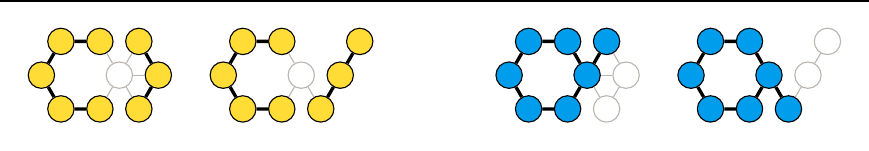
\begin{tikzpicture}[scale=0.33]%{{{
        \begin{scope}[rotate=90]
            \node[draw, circle, fill=uofgsunshine, inner sep=0.5pt, font=\normalsize] (M1) at (90:1.5) {\phantom{0}};
            \node[draw, circle, fill=uofgsunshine, inner sep=0.5pt, font=\normalsize] (M2) at (150:1.5) {\phantom{0}};
            \node[draw, circle, fill=uofgsunshine, inner sep=0.5pt, font=\normalsize] (M3) at (30:1.5) {\phantom{0}};
            \node[draw, circle, fill=uofgsunshine, inner sep=0.5pt, font=\normalsize] (M4) at (210:1.5) {\phantom{0}};
            \node[draw, circle, fill=uofgsunshine, inner sep=0.5pt, font=\normalsize] (M5) at (330:1.5) {\phantom{0}};
            \node[draw, circle, draw=uofgsandstone!40, fill=white, inner sep=0.5pt, font=\normalsize] (M6) at (270:1.5) {\phantom{0}};
            \node[draw, circle, fill=uofgsunshine, inner sep=0.5pt, font=\normalsize] (M7) at ($(210:1.5) + (M6)$) {\phantom{0}};
            \node[draw, circle, fill=uofgsunshine, inner sep=0.5pt, font=\normalsize] (M8) at ($(330:1.5) + (M6)$) {\phantom{0}};
            \node[draw, circle, fill=uofgsunshine, inner sep=0.5pt, font=\normalsize] (M9) at ($(270:1.5) + (M6)$) {\phantom{0}};

            \draw [very thick] (M1) -- (M2);
            \draw [very thick] (M2) -- (M4);
            \draw [very thick] (M3) -- (M5);
            \draw [color=uofgsandstone!40] (M4) -- (M6);
            \draw [color=uofgsandstone!40] (M5) -- (M6);
            \draw [very thick] (M3) -- (M1);
            \draw [color=uofgsandstone!40] (M6) -- (M7);
            \draw [color=uofgsandstone!40] (M6) -- (M8);
            \draw [color=uofgsandstone!40] (M6) -- (M9);
            \draw [very thick] (M7) -- (M9);
            \draw [very thick] (M8) -- (M9);
        \end{scope}

        \begin{scope}[xshift=7cm, rotate=90]
            \node[draw, circle, fill=uofgsunshine, inner sep=0.5pt, font=\normalsize] (M1) at (90:1.5) {\phantom{0}};
            \node[draw, circle, fill=uofgsunshine, inner sep=0.5pt, font=\normalsize] (M2) at (150:1.5) {\phantom{0}};
            \node[draw, circle, fill=uofgsunshine, inner sep=0.5pt, font=\normalsize] (M3) at (30:1.5) {\phantom{0}};
            \node[draw, circle, fill=uofgsunshine, inner sep=0.5pt, font=\normalsize] (M4) at (210:1.5) {\phantom{0}};
            \node[draw, circle, fill=uofgsunshine, inner sep=0.5pt, font=\normalsize] (M5) at (330:1.5) {\phantom{0}};
            \node[draw, circle, draw=uofgsandstone!40, fill=white, inner sep=0.5pt, font=\normalsize] (M6) at (270:1.5) {\phantom{0}};
            \node[draw, circle, fill=uofgsunshine, inner sep=0.5pt, font=\normalsize] (M7) at ($(210:1.5) + (M6)$) {\phantom{0}};
            \node[draw, circle, fill=uofgsunshine, inner sep=0.5pt, font=\normalsize] (M8) at ($(270:1.5) + (M6)$) {\phantom{0}};
            \node[draw, circle, fill=uofgsunshine, inner sep=0.5pt, font=\normalsize] (M9) at ($(330:1.5) + (M8)$) {\phantom{0}};

            \draw [very thick] (M1) -- (M2);
            \draw [very thick] (M2) -- (M4);
            \draw [very thick] (M3) -- (M5);
            \draw [color=uofgsandstone!40] (M4) -- (M6);
            \draw [color=uofgsandstone!40] (M5) -- (M6);
            \draw [very thick] (M3) -- (M1);
            \draw [color=uofgsandstone!40] (M6) -- (M7);
            \draw [very thick] (M7) -- (M8);
            \draw [very thick] (M8) -- (M9);
        \end{scope}

        \begin{scope}[xshift=18cm, rotate=90]
            \node[draw, circle, fill=uofgcobalt, inner sep=0.5pt, font=\normalsize] (M1) at (90:1.5) {\phantom{0}};
            \node[draw, circle, fill=uofgcobalt, inner sep=0.5pt, font=\normalsize] (M2) at (150:1.5) {\phantom{0}};
            \node[draw, circle, fill=uofgcobalt, inner sep=0.5pt, font=\normalsize] (M3) at (30:1.5) {\phantom{0}};
            \node[draw, circle, fill=uofgcobalt, inner sep=0.5pt, font=\normalsize] (M4) at (210:1.5) {\phantom{0}};
            \node[draw, circle, fill=uofgcobalt, inner sep=0.5pt, font=\normalsize] (M5) at (330:1.5) {\phantom{0}};
            \node[draw, circle, fill=uofgcobalt, inner sep=0.5pt, font=\normalsize] (M6) at (270:1.5) {\phantom{0}};
            \node[draw, circle, draw=uofgsandstone!40, fill=white, inner sep=0.5pt, font=\normalsize] (M7) at ($(210:1.5) + (M6)$) {\phantom{0}};
            \node[draw, circle, fill=uofgcobalt, inner sep=0.5pt, font=\normalsize] (M8) at ($(330:1.5) + (M6)$) {\phantom{0}};
            \node[draw, circle, draw=uofgsandstone!40, fill=white, inner sep=0.5pt, font=\normalsize] (M9) at ($(270:1.5) + (M6)$) {\phantom{0}};

            \draw [very thick] (M1) -- (M2);
            \draw [very thick] (M2) -- (M4);
            \draw [very thick] (M3) -- (M5);
            \draw [very thick] (M4) -- (M6);
            \draw [very thick] (M5) -- (M6);
            \draw [very thick] (M3) -- (M1);
            \draw [color=uofgsandstone!40] (M6) -- (M7);
            \draw [very thick] (M6) -- (M8);
            \draw [color=uofgsandstone!40] (M6) -- (M9);
            \draw [color=uofgsandstone!40] (M7) -- (M9);
            \draw [color=uofgsandstone!40] (M8) -- (M9);
        \end{scope}

        \begin{scope}[xshift=25cm, rotate=90]
            \node[draw, circle, fill=uofgcobalt, inner sep=0.5pt, font=\normalsize] (M1) at (90:1.5) {\phantom{0}};
            \node[draw, circle, fill=uofgcobalt, inner sep=0.5pt, font=\normalsize] (M2) at (150:1.5) {\phantom{0}};
            \node[draw, circle, fill=uofgcobalt, inner sep=0.5pt, font=\normalsize] (M3) at (30:1.5) {\phantom{0}};
            \node[draw, circle, fill=uofgcobalt, inner sep=0.5pt, font=\normalsize] (M4) at (210:1.5) {\phantom{0}};
            \node[draw, circle, fill=uofgcobalt, inner sep=0.5pt, font=\normalsize] (M5) at (330:1.5) {\phantom{0}};
            \node[draw, circle, fill=uofgcobalt, inner sep=0.5pt, font=\normalsize] (M6) at (270:1.5) {\phantom{0}};
            \node[draw, circle, fill=uofgcobalt, inner sep=0.5pt, font=\normalsize] (M7) at ($(210:1.5) + (M6)$) {\phantom{0}};
            \node[draw, circle, draw=uofgsandstone!40, fill=white, inner sep=0.5pt, font=\normalsize] (M8) at ($(270:1.5) + (M6)$) {\phantom{0}};
            \node[draw, circle, draw=uofgsandstone!40, fill=white, inner sep=0.5pt, font=\normalsize] (M9) at ($(330:1.5) + (M8)$) {\phantom{0}};

            \draw [very thick] (M1) -- (M2);
            \draw [very thick] (M2) -- (M4);
            \draw [very thick] (M3) -- (M5);
            \draw [very thick] (M4) -- (M6);
            \draw [very thick] (M5) -- (M6);
            \draw [very thick] (M3) -- (M1);
            \draw [very thick] (M6) -- (M7);
            \draw [draw=uofgsandstone!40] (M7) -- (M8);
            \draw [draw=uofgsandstone!40] (M8) -- (M9);
        \end{scope}
\end{tikzpicture}
\caption{A maximum common induced subgraph of the first two graphs has eight vertices, shaded.
However, if we require the common subgraph to be connected, only seven vertices may be
selected---one way to do this is shown in the third and fourth graphs.}\label{figure:mcsexample}
\end{figure}

Maximum common subgraph problems arise in biology and chemistry
\cite{DBLP:journals/jcamd/RaymondW02a,Ehrlich:2011}, in computer vision
\cite{DBLP:journals/jair/CookH94}, in the analysis of source code
\cite{DBLP:journals/tkde/DjokoCH97}, binary programs \cite{DBLP:conf/icics/GaoRS08}, and circuit
designs \cite{DBLP:journals/jair/CookH94}, in character recognition problems \cite{SIWEILU1991617},
and in many other domains \cite{Shasha:2002:AAT:543613.543620}, both directly and as a way of
measuring the similarity or difference between two graphs
\cite{DBLP:journals/prl/Bunke97,DBLP:journals/prl/FernandezV01,KriegeThesis}. We illustrate two
variants of the problem in \cref{figure:mcsexample}.

Throughout this paper we will be working with graphs which may be directed, which may have labels
associated with vertices, edges, or both, and which may contain loops. To simplify notation, we will
work with a very broad definition: we define a \emph{graph} $G = (V, \ell, e)$ to be a set of
vertices $V$, a vertex labelling function $\ell : V \rightarrow \mathbb{N}$, and an edge labelling
function $e : V \times V \rightarrow \mathbb{N} \cup \{ \bot \}$. To represent graphs without vertex
(or edge) labels, we just pick our favourite number and give it to every vertex (or edge). We also
use a distinct label $\bot$ to represent the \emph{lack of} an edge between two vertices; vertices
$v$ and $w$ are said to be \emph{adjacent} if $e(v, w) \ne \bot$ or $e(w, v) \ne \bot$. We write
$\operatorname{V}(G)$ for $V$, and $\operatorname{N}(G, v)$ for the \emph{undirected neighbourhood}
of a vertex $v$ (that is, the set of vertices adjacent to $v$); a vertex is \emph{isolated} if its
neighbourhood is empty. A (weak) \emph{path} between two vertices $v$ and $w$ is a sequence of $n$
vertices $v = v_1, v_2, \ldots, v_n = w$ such that for each $m \in \{ 1 \ldots n - 1 \}$, $v_m$ is
adjacent to $v_{m + 1}$. A graph is (weakly) \emph{connected} if a path exists between each distinct
pair of vertices.

Given two graphs $G_1 = (V_1, \ell_1, e_1)$ and $G_2 = (V_2, \ell_2, e_2)$, we say two pairs of
vertices $(v_1, w_1) \in \operatorname{V}(G_1) \times \operatorname{V}(G_1)$ and $(v_2, w_2) \in
\operatorname{V}(G_2) \times \operatorname{V}(G_2)$ are \emph{compatible}, written $(v_1, w_1)
\simeq (v_2, w_2)$, if both $e_1(v_1, w_1) = e_2(v_2, w_2)$ and $e_1(w_1, v_1) = e_2(w_2, v_2)$. We
say two vertices $v \in \operatorname{V}(G_1)$ and $w \in \operatorname{V}(G_2)$ are
\emph{compatible}, written $v \simeq w$, if $\ell_1(v) = \ell_2(w)$ and $(v, v) \simeq (w, w)$.

An \emph{induced subgraph isomorphism} from a graph $G$ to a graph $H$ is an injective function $i :
\operatorname{V}(G) \rightarrow \operatorname{V}(H)$ such that for every vertex $v \in
\operatorname{V}(G)$, $v \simeq i(v)$, and for every pair of vertices $(v, w) \in
\operatorname{V}(G) \times \operatorname{V}(G)$, $(v, w) \simeq (i(v), i(w))$. A \emph{common
induced subgraph isomorphism} between two graphs $G_1$ and $G_2$ is a graph $G$, together with a
pair of induced subgraph isomorphisms $i_1 : G \rightarrow G_1$ and $i_2 : G \rightarrow G_2$. A
\emph{common induced subgraph} of $G_1$ and $G_2$ is a graph $G$ which has a common subgraph
isomorphism to $G_1$ and $G_2$. A \emph{maximum common (connected) induced subgraph} is a common
(connected) induced subgraph with the largest possible number of vertices.  (The distinction between
a common subgraph and a common subgraph isomorphism is relevant when counting distinct solutions,
which we do not consider in this paper; in \cref{figure:mcsexample} on the left, there is only one
maximum common subgraph, but four different maximum common subgraph isomorphisms are possible.)

There is also a non-induced version of these problems, which is commonly known as the \emph{maximum
common partial subgraph} problem: here, if $e(v, w) = \bot$, then $e_1(i_1(v), i_1(w))$ and
$e_2(i_2(v), i_2(w))$ may take any value, and we must maximise the number of non-$\bot$ vertex pairs
(i.e.\ edges) in $G$ instead (it is not entirely clear what the objective should be in directed
graphs, or when loops are present). We restrict ourselves to the induced version in this paper.

\subsection{Existing Approaches}

One approach to maximum common subgraph problems is via constraint programming
\cite{DBLP:conf/mco/VismaraV08,DBLP:conf/cp/NdiayeS11}. The models are based upon constructing an
injective mapping from the vertices of one graph (typically the smaller) to the other, in a similar
manner to subgraph isomorphism algorithms
\cite{DBLP:journals/ai/Solnon10,DBLP:conf/cp/AudemardLMGP14,DBLP:conf/cp/McCreeshP15}. However, to
allow for a partial mapping, a special $\bot$ value is added to each domain (and so we are
constructing a maximum common subgraph isomorphism, where the common subgraph is implicitly the
subgraph of the first graph given by taking the vertices which are not assigned to $\bot$, and the
first subgraph isomorphism is the inclusion map). The objective is then to minimise the number of
variables given the $\bot$ value---for best results, a special propagator for the injectivity
condition is used, which simultaneously enforces that all variables taking non-$\bot$ are different,
and restricts the number of $\bot$ values which may be used based upon the objective
\cite{DBLP:conf/cp/PetitRB01}.  Unfortunately, the addition of $\bot$ also invalidates many of the
invariants used for subgraph isomorphism---we may no longer reason using the degree of vertices, for
example, and so maximum common subgraph problems can be much more challenging in practice.

Another widely studied approach ?? cite is to reduce the problem to finding a maximum clique (or sometimes,
equivalently, an independent set or a vertex cover ?? cite) in an association graph \cite{LeviG}; we describe
this below. Conventional wisdom is that this approach is less effective in practice, but previous
experimental evaluations have used weak clique algorithms, or even maximal clique enumeration
algorithms. Maximum clique algorithms are an active research area
\cite{DBLP:conf/dmtcs/TomitaS03,DBLP:journals/jgo/TomitaK07,DBLP:conf/walcom/TomitaSHTW10,DBLP:journals/cor/SegundoRJ11,DBLP:journals/algorithms/Prosser12,DBLP:journals/ol/SegundoMRH13,DBLP:conf/ictai/LiFX13,DBLP:journals/cor/SegundoT14,DBLP:conf/lion/SegundoLB14,DBLP:conf/cp/McCreeshP14,DBLP:journals/jco/BatsynGMP14,DBLP:journals/cor/SegundoNB15,DBLP:conf/lion/NikolaevBS15,DBLP:conf/lion/LiJX15,DBLP:journals/jcc/KoncDTRJ12,DBLP:journals/algorithms/McCreeshP13,DBLP:journals/topc/McCreeshP15,DBLP:journals/cor/SegundoLP16},
and so the first half of this paper re-evaluates the association graph approach using a modern
algorithm.

(Other approaches have been tried, including dedicated algorithms ?? cite, mixed integer programming
\cite{DBLP:journals/anor/PivaS12}, and heuristics \cite{DBLP:journals/jcisd/EnglertK15}; SAT
encodings seem to struggle even for subgraph isomorphism \cite{UpcomingIJCAIPaper}.)

An interesting variant of the maximum common subgraph problem requires the selected subgraph to be
connected
\cite{DBLP:journals/tcs/Koch01,DBLP:journals/jcamd/RaymondW02a,DBLP:conf/mco/VismaraV08,Ehrlich:2011}.
Adding the connectedness requirement makes certain special cases solvable in polynomial time,
including outerplanar graphs of bounded degree \cite{DBLP:journals/algorithms/AkutsuT13} and trees
\cite{DBLP:journals/corr/DroschinskyKM16}, but the general case remains \NP-hard. The second half of
this paper looks at this variant on arbitrary graphs. In principle, for a constraint programming
approach, we may simply add a ``forms a connected graph'' global constraint
\cite{Brown:2005,DBLP:conf/cp/DoomsDD05,DBLP:conf/cp/QuesadaRD05} to the model. Alternatively, we
could use a special branching rule to maintain connectedness during search ?? cite. Neither approach
seems directly viable with an association graph encoding---however, we show that it is possible to
adapt the combined branching and bounding rule used by modern clique algorithms to preserve
connectedness during search.

Our experiments suggest that each approach gives broadly similar performance, although the
association graph works better when graphs have edge labels (and we can explain why), and the
constraint programming approach is better when edges are unlabelled. For the constraint programming
model, using both a global constraint \emph{and} the branching rule in conjunction seems to be the
safest option---although it is not always fastest, it is very rarely substantially worse than just
using one or the other, and is often substantially better.

\subsection{Datasets}

\cite{DBLP:journals/prl/SantoFSV03,DBLP:journals/jgaa/ConteFV07}

?? More? Can we scale to some of the SIP graphs?

\section{Re-Evaluating the Clique Model}

Previous experimental work has used a maximal clique enumeration algorithm, even for the
maximisation problem. ?? check this! I recall someone using a bad max clique algorithm too.
\cite{DBLP:conf/sspr/BunkeFGSV02,DBLP:journals/jgaa/ConteFV07}

We instead use a maximum clique algorithm.

Also sparse stuff, but association graphs aren't sparse enough.

Say which clique algorithm we're using.

\subsection{Reduction to Maximum Clique in an Association Graph}

Explain association graph \cref{figure:association}, cite history \cite{LeviG}, connections to
microstructure \cite{DBLP:conf/aaai/Jegou93a}.

Discuss how edge labels, vertex labels, directed edges, etc, are handled. Note that we can generally
only handle very local side constraints, or injectivity (which is decomposable).

\begin{figure}[tb]
    \centering
    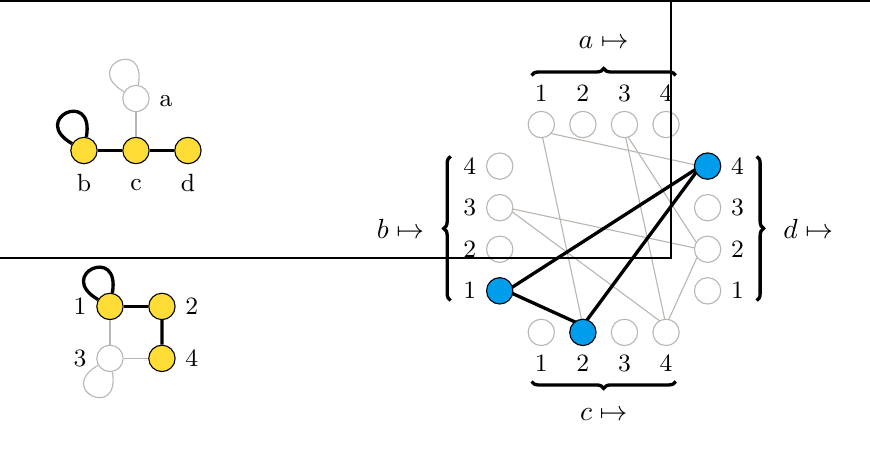
\begin{tikzpicture}[scale=0.33]%{{{
        \begin{scope}
            \node[draw, circle, fill=white, draw=uofgsandstone!40, inner sep=0.5pt, font=\normalsize] (Ma) at (2, 10) {\phantom{0}};
            \node[draw, circle, fill=uofgsunshine, inner sep=0.5pt, font=\normalsize] (Mb) at (0, 8) {\phantom{0}};
            \node[draw, circle, fill=uofgsunshine, inner sep=0.5pt, font=\normalsize] (Mc) at (2, 8) {\phantom{0}};
            \node[draw, circle, fill=uofgsunshine, inner sep=0.5pt, font=\normalsize] (Md) at (4, 8) {\phantom{0}};

            \node [right = 0 of Ma, font=\small] { \vphantom{0}a };
            \node [below = 0 of Mb, font=\small] { \vphantom{0}b };
            \node [below = 0 of Mc, font=\small] { \vphantom{0}c };
            \node [below = 0 of Md, font=\small] { \vphantom{0}d };

            \draw [very thick] (Mb) -- (Mc);
            \draw [very thick] (Mc) -- (Md);
            \draw [color=uofgsandstone!40] (Ma) -- (Mc);
            \draw [color=uofgsandstone!40] (Ma) to [out=150, in=80, looseness=8] (Ma);
            \draw [very thick] (Mb) to [out=150, in=80, looseness=8] (Mb);
        \end{scope}

        \begin{scope}
            \node[draw, circle, fill=uofgsunshine, inner sep=0.5pt, font=\normalsize] (M1) at (1, 2) {\phantom{0}};
            \node[draw, circle, fill=uofgsunshine, inner sep=0.5pt, font=\normalsize] (M2) at (3, 2) {\phantom{0}};
            \node[draw, circle, fill=white, draw=uofgsandstone!40, inner sep=0.5pt, font=\normalsize] (M3) at (1, 0) {\phantom{0}};
            \node[draw, circle, fill=uofgsunshine, inner sep=0.5pt, font=\normalsize] (M4) at (3, 0) {\phantom{0}};

            \node [left = 0 of M1, font=\small] { \vphantom{0}1 };
            \node [right = 0 of M2, font=\small] { \vphantom{0}2 };
            \node [left = 0 of M3, font=\small] { \vphantom{0}3 };
            \node [right = 0 of M4, font=\small] { \vphantom{0}4 };

            \draw [very thick] (M1) -- (M2);
            \draw [very thick] (M2) -- (M4);
            \draw [color=uofgsandstone!40] (M3) -- (M4);
            \draw [color=uofgsandstone!40] (M1) -- (M3);

            \draw [color=uofgsandstone!40] (M3) to [out=280, in=210, looseness=8] (M3);
            \draw [very thick] (M1) to [out=150, in=80, looseness=8] (M1);
        \end{scope}

        \begin{scope}[xshift=15cm]
            \node[draw, circle, fill=white, draw=uofgsandstone!40, inner sep=0.5pt, font=\normalsize] (Ma1) at (2.6, 9) {\phantom{0}};
            \node[draw, circle, fill=white, draw=uofgsandstone!40, inner sep=0.5pt, font=\normalsize] (Ma2) at (4.2, 9) {\phantom{0}};
            \node[draw, circle, fill=white, draw=uofgsandstone!40, inner sep=0.5pt, font=\normalsize] (Ma3) at (5.8, 9) {\phantom{0}};
            \node[draw, circle, fill=white, draw=uofgsandstone!40, inner sep=0.5pt, font=\normalsize] (Ma4) at (7.4, 9) {\phantom{0}};
            \node [above = 0 of Ma1, font=\small] { \vphantom{0}1 };
            \node [above = 0 of Ma2, font=\small] { \vphantom{0}2 };
            \node [above = 0 of Ma3, font=\small] { \vphantom{0}3 };
            \node [above = 0 of Ma4, font=\small] { \vphantom{0}4 };

            \draw [decorate, decoration={brace, raise=0.5cm}, very thick] (Ma1.north west) -- (Ma4.north east)
            node [midway, above=0.7cm] { $a \mapsto$ };

            \node[draw, circle, fill=uofgcobalt, inner sep=0.5pt, font=\normalsize] (Mb1) at (1, 2.6) {\phantom{0}};
            \node[draw, circle, fill=white, draw=uofgsandstone!40, inner sep=0.5pt, font=\normalsize] (Mb2) at (1, 4.2) {\phantom{0}};
            \node[draw, circle, fill=white, draw=uofgsandstone!40, inner sep=0.5pt, font=\normalsize] (Mb3) at (1, 5.8) {\phantom{0}};
            \node[draw, circle, fill=white, draw=uofgsandstone!40, inner sep=0.5pt, font=\normalsize] (Mb4) at (1, 7.4) {\phantom{0}};
            \node [left = 0 of Mb1, font=\small] { \vphantom{0}1 };
            \node [left = 0 of Mb2, font=\small] { \vphantom{0}2 };
            \node [left = 0 of Mb3, font=\small] { \vphantom{0}3 };
            \node [left = 0 of Mb4, font=\small] { \vphantom{0}4 };

            \draw [decorate, decoration={brace, raise=0.5cm}, very thick] (Mb1.south west) -- (Mb4.north west)
            node [midway, left=0.7cm] { $b \mapsto$ };

            \node[draw, circle, fill=white, draw=uofgsandstone!40, inner sep=0.5pt, font=\normalsize] (Mc1) at (2.6, 1) {\phantom{0}};
            \node[draw, circle, fill=uofgcobalt, inner sep=0.5pt, font=\normalsize] (Mc2) at (4.2, 1) {\phantom{0}};
            \node[draw, circle, fill=white, draw=uofgsandstone!40, inner sep=0.5pt, font=\normalsize] (Mc3) at (5.8, 1) {\phantom{0}};
            \node[draw, circle, fill=white, draw=uofgsandstone!40, inner sep=0.5pt, font=\normalsize] (Mc4) at (7.4, 1) {\phantom{0}};
            \node [below = 0 of Mc1, font=\small] { \vphantom{0}1 };
            \node [below = 0 of Mc2, font=\small] { \vphantom{0}2 };
            \node [below = 0 of Mc3, font=\small] { \vphantom{0}3 };
            \node [below = 0 of Mc4, font=\small] { \vphantom{0}4 };

            \draw [decorate, decoration={brace, raise=0.5cm}, very thick] (Mc4.south east) -- (Mc1.south west)
            node [midway, below=0.7cm] { $c \mapsto$ };

            \node[draw, circle, fill=white, draw=uofgsandstone!40, inner sep=0.5pt, font=\normalsize] (Md1) at (9, 2.6) {\phantom{0}};
            \node[draw, circle, fill=white, draw=uofgsandstone!40, inner sep=0.5pt, font=\normalsize] (Md2) at (9, 4.2) {\phantom{0}};
            \node[draw, circle, fill=white, draw=uofgsandstone!40, inner sep=0.5pt, font=\normalsize] (Md3) at (9, 5.8) {\phantom{0}};
            \node[draw, circle, fill=uofgcobalt, inner sep=0.5pt, font=\normalsize] (Md4) at (9, 7.4) {\phantom{0}};
            \node [right = 0 of Md1, font=\small] { \vphantom{0}1 };
            \node [right = 0 of Md2, font=\small] { \vphantom{0}2 };
            \node [right = 0 of Md3, font=\small] { \vphantom{0}3 };
            \node [right = 0 of Md4, font=\small] { \vphantom{0}4 };

            \draw [decorate, decoration={brace, raise=0.5cm}, very thick] (Md4.north east) -- (Md1.south east)
            node [midway, right=0.7cm] { $d \mapsto$ };

            \begin{scope}[on background layer]
                \draw [draw=uofgsandstone!40] ($(Ma1.south)!0.5!(Ma1)$) -- ($(Md4.west)!0.5!(Md4)$);
                \draw [draw=uofgsandstone!40] ($(Ma1.south)!0.5!(Ma1)$) -- ($(Mc2.north)!0.5!(Mc2)$);
                \draw [draw=uofgsandstone!40] ($(Ma3.south)!0.5!(Ma3)$) -- ($(Mc4.north)!0.5!(Mc4)$);
                \draw [draw=uofgsandstone!40] ($(Mb3.east)!0.5!(Mb3)$) -- ($(Mc4.north)!0.5!(Mc4)$);
                \draw [draw=uofgsandstone!40] ($(Md2.west)!0.5!(Md2)$) -- ($(Mc4.north)!0.5!(Mc4)$);
                \draw [draw=uofgsandstone!40] ($(Md2.west)!0.5!(Md2)$) -- ($(Ma3.south)!0.5!(Ma3)$);
                \draw [draw=uofgsandstone!40] ($(Md2.west)!0.5!(Md2)$) -- ($(Mb3.east)!0.5!(Mb3)$);
                \draw [very thick] ($(Mb1.east)!0.5!(Mb1)$) -- ($(Mc2.north)!0.5!(Mc2)$);
                \draw [very thick] ($(Mb1.east)!0.5!(Mb1)$) -- ($(Md4.west)!0.5!(Md4)$);
                \draw [very thick] ($(Mc2.north)!0.5!(Mc2)$) -- ($(Md4.west)!0.5!(Md4)$);
        \end{scope}
        \end{scope}

    \end{tikzpicture}

    \caption{A maximum common induced subgraph between the two graphs on the left has three
        vertices---one solution is highlighted. On the right, the association graph encoding: the
        highlighted clique of size three shows the same solution. In practice the isolated vertices
        (corresponding to assignments between incompatible vertices, which are unary constraints) would be
        omitted.}\label{figure:association}
\end{figure}

?? Discuss the partial version briefly, cite the reduction.

\subsection{Experimental Evaluation}

?? Break this down more by family, size, etc.

\begin{figure}[p]
    \centering
    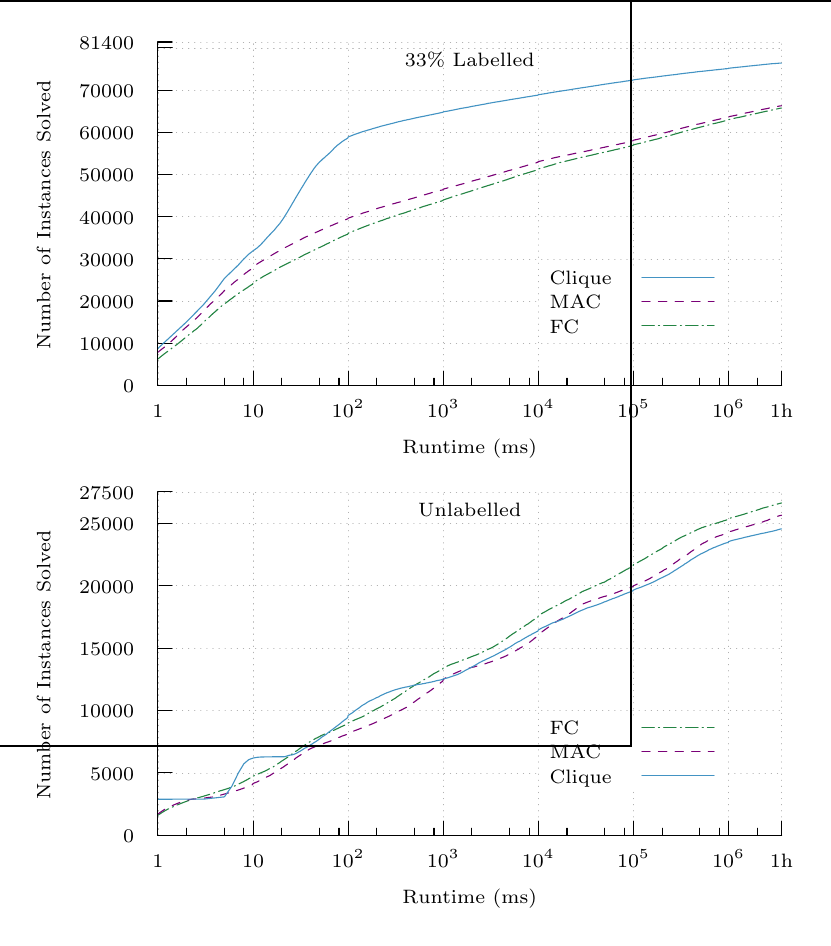
\begin{tikzpicture}[gnuplot]
%% generated with GNUPLOT 5.0p0 (Lua 5.2; terminal rev. 99, script rev. 100)
%% Tue 19 Apr 2016 16:47:15 AEST
\tikzset{every node/.append style={font={\scriptsize}}}
% \path (0.000,0.000) rectangle (10.160,11.430);
\gpcolor{color=gp lt color axes}
\gpsetlinetype{gp lt axes}
\gpsetdashtype{gp dt axes}
\gpsetlinewidth{0.50}
\draw[gp path] (1.688,10.986)--(9.607,10.986);
\gpcolor{color=gp lt color border}
\gpsetlinetype{gp lt border}
\gpsetdashtype{gp dt solid}
\gpsetlinewidth{1.00}
\draw[gp path] (1.688,10.986)--(1.868,10.986);
\gpcolor{color=gp lt color axes}
\gpsetlinetype{gp lt axes}
\gpsetdashtype{gp dt axes}
\gpsetlinewidth{0.50}
\draw[gp path] (1.688,11.061)--(9.607,11.061);
\gpcolor{color=gp lt color border}
\gpsetlinetype{gp lt border}
\gpsetdashtype{gp dt solid}
\gpsetlinewidth{1.00}
\draw[gp path] (1.688,11.061)--(1.868,11.061);
\node[gp node right] at (1.504,11.061) {81400};
\gpcolor{color=gp lt color axes}
\gpsetlinetype{gp lt axes}
\gpsetdashtype{gp dt axes}
\gpsetlinewidth{0.50}
\draw[gp path] (1.688,6.700)--(9.607,6.700);
\gpcolor{color=gp lt color border}
\gpsetlinetype{gp lt border}
\gpsetdashtype{gp dt solid}
\gpsetlinewidth{1.00}
\draw[gp path] (1.688,6.700)--(1.868,6.700);
\node[gp node right] at (1.504,6.700) {$0$};
\gpcolor{color=gp lt color axes}
\gpsetlinetype{gp lt axes}
\gpsetdashtype{gp dt axes}
\gpsetlinewidth{0.50}
\draw[gp path] (1.688,7.236)--(9.607,7.236);
\gpcolor{color=gp lt color border}
\gpsetlinetype{gp lt border}
\gpsetdashtype{gp dt solid}
\gpsetlinewidth{1.00}
\draw[gp path] (1.688,7.236)--(1.868,7.236);
\node[gp node right] at (1.504,7.236) {$10000$};
\gpcolor{color=gp lt color axes}
\gpsetlinetype{gp lt axes}
\gpsetdashtype{gp dt axes}
\gpsetlinewidth{0.50}
\draw[gp path] (1.688,7.771)--(6.546,7.771);
\draw[gp path] (8.934,7.771)--(9.607,7.771);
\gpcolor{color=gp lt color border}
\gpsetlinetype{gp lt border}
\gpsetdashtype{gp dt solid}
\gpsetlinewidth{1.00}
\draw[gp path] (1.688,7.771)--(1.868,7.771);
\node[gp node right] at (1.504,7.771) {$20000$};
\gpcolor{color=gp lt color axes}
\gpsetlinetype{gp lt axes}
\gpsetdashtype{gp dt axes}
\gpsetlinewidth{0.50}
\draw[gp path] (1.688,8.307)--(9.607,8.307);
\gpcolor{color=gp lt color border}
\gpsetlinetype{gp lt border}
\gpsetdashtype{gp dt solid}
\gpsetlinewidth{1.00}
\draw[gp path] (1.688,8.307)--(1.868,8.307);
\node[gp node right] at (1.504,8.307) {$30000$};
\gpcolor{color=gp lt color axes}
\gpsetlinetype{gp lt axes}
\gpsetdashtype{gp dt axes}
\gpsetlinewidth{0.50}
\draw[gp path] (1.688,8.843)--(9.607,8.843);
\gpcolor{color=gp lt color border}
\gpsetlinetype{gp lt border}
\gpsetdashtype{gp dt solid}
\gpsetlinewidth{1.00}
\draw[gp path] (1.688,8.843)--(1.868,8.843);
\node[gp node right] at (1.504,8.843) {$40000$};
\gpcolor{color=gp lt color axes}
\gpsetlinetype{gp lt axes}
\gpsetdashtype{gp dt axes}
\gpsetlinewidth{0.50}
\draw[gp path] (1.688,9.379)--(9.607,9.379);
\gpcolor{color=gp lt color border}
\gpsetlinetype{gp lt border}
\gpsetdashtype{gp dt solid}
\gpsetlinewidth{1.00}
\draw[gp path] (1.688,9.379)--(1.868,9.379);
\node[gp node right] at (1.504,9.379) {$50000$};
\gpcolor{color=gp lt color axes}
\gpsetlinetype{gp lt axes}
\gpsetdashtype{gp dt axes}
\gpsetlinewidth{0.50}
\draw[gp path] (1.688,9.914)--(9.607,9.914);
\gpcolor{color=gp lt color border}
\gpsetlinetype{gp lt border}
\gpsetdashtype{gp dt solid}
\gpsetlinewidth{1.00}
\draw[gp path] (1.688,9.914)--(1.868,9.914);
\node[gp node right] at (1.504,9.914) {$60000$};
\gpcolor{color=gp lt color axes}
\gpsetlinetype{gp lt axes}
\gpsetdashtype{gp dt axes}
\gpsetlinewidth{0.50}
\draw[gp path] (1.688,10.450)--(9.607,10.450);
\gpcolor{color=gp lt color border}
\gpsetlinetype{gp lt border}
\gpsetdashtype{gp dt solid}
\gpsetlinewidth{1.00}
\draw[gp path] (1.688,10.450)--(1.868,10.450);
\node[gp node right] at (1.504,10.450) {$70000$};
\gpcolor{color=gp lt color axes}
\gpsetlinetype{gp lt axes}
\gpsetdashtype{gp dt axes}
\gpsetlinewidth{0.50}
\draw[gp path] (1.688,10.986)--(9.607,10.986);
\gpcolor{color=gp lt color border}
\gpsetlinetype{gp lt border}
\gpsetdashtype{gp dt solid}
\gpsetlinewidth{1.00}
\draw[gp path] (1.688,10.986)--(1.868,10.986);
\gpcolor{color=gp lt color axes}
\gpsetlinetype{gp lt axes}
\gpsetdashtype{gp dt axes}
\gpsetlinewidth{0.50}
\draw[gp path] (1.688,6.700)--(1.688,11.061);
\gpcolor{color=gp lt color border}
\gpsetlinetype{gp lt border}
\gpsetdashtype{gp dt solid}
\gpsetlinewidth{1.00}
\draw[gp path] (1.688,6.700)--(1.688,6.880);
\node[gp node center] at (1.688,6.392) {1};
\gpcolor{color=gp lt color axes}
\gpsetlinetype{gp lt axes}
\gpsetdashtype{gp dt axes}
\gpsetlinewidth{0.50}
\draw[gp path] (2.896,6.700)--(2.896,11.061);
\gpcolor{color=gp lt color border}
\gpsetlinetype{gp lt border}
\gpsetdashtype{gp dt solid}
\gpsetlinewidth{1.00}
\draw[gp path] (2.896,6.700)--(2.896,6.880);
\node[gp node center] at (2.896,6.392) {10};
\gpcolor{color=gp lt color axes}
\gpsetlinetype{gp lt axes}
\gpsetdashtype{gp dt axes}
\gpsetlinewidth{0.50}
\draw[gp path] (9.607,6.700)--(9.607,11.061);
\gpcolor{color=gp lt color border}
\gpsetlinetype{gp lt border}
\gpsetdashtype{gp dt solid}
\gpsetlinewidth{1.00}
\draw[gp path] (9.607,6.700)--(9.607,6.880);
\node[gp node center] at (9.607,6.392) {1h};
\gpcolor{color=gp lt color axes}
\gpsetlinetype{gp lt axes}
\gpsetdashtype{gp dt axes}
\gpsetlinewidth{0.50}
\draw[gp path] (1.688,6.700)--(1.688,11.061);
\gpcolor{color=gp lt color border}
\gpsetlinetype{gp lt border}
\gpsetdashtype{gp dt solid}
\gpsetlinewidth{1.00}
\draw[gp path] (1.688,6.700)--(1.688,6.880);
\draw[gp path] (2.052,6.700)--(2.052,6.790);
\draw[gp path] (2.532,6.700)--(2.532,6.790);
\draw[gp path] (2.779,6.700)--(2.779,6.790);
\gpcolor{color=gp lt color axes}
\gpsetlinetype{gp lt axes}
\gpsetdashtype{gp dt axes}
\gpsetlinewidth{0.50}
\draw[gp path] (2.896,6.700)--(2.896,11.061);
\gpcolor{color=gp lt color border}
\gpsetlinetype{gp lt border}
\gpsetdashtype{gp dt solid}
\gpsetlinewidth{1.00}
\draw[gp path] (2.896,6.700)--(2.896,6.880);
\draw[gp path] (3.259,6.700)--(3.259,6.790);
\draw[gp path] (3.740,6.700)--(3.740,6.790);
\draw[gp path] (3.987,6.700)--(3.987,6.790);
\gpcolor{color=gp lt color axes}
\gpsetlinetype{gp lt axes}
\gpsetdashtype{gp dt axes}
\gpsetlinewidth{0.50}
\draw[gp path] (4.104,6.700)--(4.104,11.061);
\gpcolor{color=gp lt color border}
\gpsetlinetype{gp lt border}
\gpsetdashtype{gp dt solid}
\gpsetlinewidth{1.00}
\draw[gp path] (4.104,6.700)--(4.104,6.880);
\node[gp node center] at (4.104,6.392) {$10^{2}$};
\draw[gp path] (4.467,6.700)--(4.467,6.790);
\draw[gp path] (4.948,6.700)--(4.948,6.790);
\draw[gp path] (5.194,6.700)--(5.194,6.790);
\gpcolor{color=gp lt color axes}
\gpsetlinetype{gp lt axes}
\gpsetdashtype{gp dt axes}
\gpsetlinewidth{0.50}
\draw[gp path] (5.312,6.700)--(5.312,11.061);
\gpcolor{color=gp lt color border}
\gpsetlinetype{gp lt border}
\gpsetdashtype{gp dt solid}
\gpsetlinewidth{1.00}
\draw[gp path] (5.312,6.700)--(5.312,6.880);
\node[gp node center] at (5.312,6.392) {$10^{3}$};
\draw[gp path] (5.675,6.700)--(5.675,6.790);
\draw[gp path] (6.156,6.700)--(6.156,6.790);
\draw[gp path] (6.402,6.700)--(6.402,6.790);
\gpcolor{color=gp lt color axes}
\gpsetlinetype{gp lt axes}
\gpsetdashtype{gp dt axes}
\gpsetlinewidth{0.50}
\draw[gp path] (6.519,6.700)--(6.519,11.061);
\gpcolor{color=gp lt color border}
\gpsetlinetype{gp lt border}
\gpsetdashtype{gp dt solid}
\gpsetlinewidth{1.00}
\draw[gp path] (6.519,6.700)--(6.519,6.880);
\node[gp node center] at (6.519,6.392) {$10^{4}$};
\draw[gp path] (6.883,6.700)--(6.883,6.790);
\draw[gp path] (7.364,6.700)--(7.364,6.790);
\draw[gp path] (7.610,6.700)--(7.610,6.790);
\gpcolor{color=gp lt color axes}
\gpsetlinetype{gp lt axes}
\gpsetdashtype{gp dt axes}
\gpsetlinewidth{0.50}
\draw[gp path] (7.727,6.700)--(7.727,7.302);
\draw[gp path] (7.727,8.226)--(7.727,11.061);
\gpcolor{color=gp lt color border}
\gpsetlinetype{gp lt border}
\gpsetdashtype{gp dt solid}
\gpsetlinewidth{1.00}
\draw[gp path] (7.727,6.700)--(7.727,6.880);
\node[gp node center] at (7.727,6.392) {$10^{5}$};
\draw[gp path] (8.091,6.700)--(8.091,6.790);
\draw[gp path] (8.571,6.700)--(8.571,6.790);
\draw[gp path] (8.818,6.700)--(8.818,6.790);
\gpcolor{color=gp lt color axes}
\gpsetlinetype{gp lt axes}
\gpsetdashtype{gp dt axes}
\gpsetlinewidth{0.50}
\draw[gp path] (8.935,6.700)--(8.935,11.061);
\gpcolor{color=gp lt color border}
\gpsetlinetype{gp lt border}
\gpsetdashtype{gp dt solid}
\gpsetlinewidth{1.00}
\draw[gp path] (8.935,6.700)--(8.935,6.880);
\node[gp node center] at (8.935,6.392) {$10^{6}$};
\draw[gp path] (9.299,6.700)--(9.299,6.790);
\draw[gp path] (1.688,11.061)--(1.688,6.700)--(9.607,6.700);
\node[gp node center,rotate=-270] at (0.246,8.880) {Number of Instances Solved};
\node[gp node center] at (5.647,5.930) {Runtime (ms)};
\node[gp node left] at (6.546,8.072) {Clique};
\gpcolor{rgb color={0.263,0.576,0.765}}
\draw[gp path] (7.834,8.072)--(8.750,8.072);
\draw[gp path] (1.688,7.170)--(2.052,7.507)--(2.264,7.723)--(2.415,7.901)--(2.532,8.058)%
  --(2.628,8.151)--(2.709,8.229)--(2.779,8.306)--(2.841,8.366)--(2.896,8.409)--(2.946,8.444)%
  --(2.991,8.485)--(3.033,8.530)--(3.072,8.574)--(3.109,8.614)--(3.142,8.648)--(3.174,8.682)%
  --(3.204,8.720)--(3.233,8.752)--(3.259,8.789)--(3.285,8.826)--(3.309,8.865)--(3.333,8.903)%
  --(3.355,8.941)--(3.376,8.976)--(3.397,9.013)--(3.417,9.046)--(3.436,9.080)--(3.454,9.110)%
  --(3.472,9.140)--(3.489,9.168)--(3.506,9.197)--(3.522,9.222)--(3.538,9.248)--(3.553,9.274)%
  --(3.568,9.298)--(3.582,9.320)--(3.596,9.341)--(3.610,9.364)--(3.623,9.385)--(3.636,9.404)%
  --(3.649,9.422)--(3.661,9.441)--(3.673,9.458)--(3.685,9.473)--(3.696,9.487)--(3.708,9.501)%
  --(3.719,9.513)--(3.729,9.524)--(3.740,9.537)--(3.750,9.546)--(3.761,9.555)--(3.771,9.565)%
  --(3.780,9.574)--(3.790,9.582)--(3.800,9.590)--(3.809,9.598)--(3.818,9.606)--(3.827,9.615)%
  --(3.836,9.622)--(3.844,9.630)--(3.853,9.637)--(3.861,9.645)--(3.870,9.653)--(3.878,9.661)%
  --(3.886,9.668)--(3.894,9.676)--(3.901,9.684)--(3.909,9.692)--(3.917,9.701)--(3.924,9.710)%
  --(3.931,9.716)--(3.939,9.724)--(3.946,9.730)--(3.953,9.736)--(3.960,9.744)--(3.967,9.749)%
  --(3.973,9.754)--(3.980,9.759)--(3.987,9.764)--(3.993,9.769)--(4.000,9.774)--(4.006,9.779)%
  --(4.012,9.783)--(4.018,9.789)--(4.025,9.794)--(4.031,9.798)--(4.037,9.802)--(4.043,9.806)%
  --(4.048,9.809)--(4.054,9.813)--(4.060,9.817)--(4.066,9.821)--(4.071,9.823)--(4.077,9.827)%
  --(4.082,9.830)--(4.088,9.834)--(4.093,9.837)--(4.098,9.840)--(4.104,9.855)--(4.154,9.874)%
  --(4.199,9.892)--(4.241,9.905)--(4.280,9.920)--(4.316,9.930)--(4.350,9.941)--(4.382,9.949)%
  --(4.412,9.959)--(4.440,9.967)--(4.467,9.976)--(4.493,9.982)--(4.517,9.990)--(4.541,9.996)%
  --(4.563,10.002)--(4.584,10.007)--(4.605,10.013)--(4.625,10.017)--(4.644,10.023)--(4.662,10.026)%
  --(4.680,10.031)--(4.697,10.036)--(4.714,10.041)--(4.730,10.044)--(4.746,10.049)--(4.761,10.052)%
  --(4.776,10.055)--(4.790,10.059)--(4.804,10.063)--(4.818,10.066)--(4.831,10.068)--(4.844,10.070)%
  --(4.856,10.074)--(4.869,10.076)--(4.881,10.078)--(4.893,10.081)--(4.904,10.084)--(4.915,10.086)%
  --(4.927,10.089)--(4.937,10.091)--(4.948,10.094)--(4.958,10.096)--(4.969,10.099)--(4.979,10.100)%
  --(4.988,10.103)--(4.998,10.105)--(5.007,10.107)--(5.017,10.108)--(5.026,10.111)--(5.035,10.112)%
  --(5.044,10.114)--(5.052,10.115)--(5.061,10.117)--(5.069,10.118)--(5.077,10.121)--(5.086,10.122)%
  --(5.094,10.124)--(5.101,10.126)--(5.109,10.127)--(5.117,10.128)--(5.124,10.130)--(5.132,10.132)%
  --(5.139,10.134)--(5.146,10.135)--(5.154,10.136)--(5.161,10.137)--(5.168,10.139)--(5.174,10.140)%
  --(5.181,10.142)--(5.188,10.143)--(5.194,10.145)--(5.201,10.146)--(5.207,10.147)--(5.214,10.148)%
  --(5.220,10.150)--(5.226,10.151)--(5.232,10.152)--(5.238,10.153)--(5.244,10.155)--(5.250,10.156)%
  --(5.256,10.158)--(5.262,10.159)--(5.268,10.160)--(5.273,10.161)--(5.279,10.163)--(5.285,10.164)%
  --(5.290,10.165)--(5.296,10.166)--(5.301,10.167)--(5.306,10.168)--(5.312,10.174)--(5.362,10.182)%
  --(5.407,10.191)--(5.449,10.199)--(5.488,10.207)--(5.524,10.215)--(5.558,10.221)--(5.590,10.226)%
  --(5.620,10.231)--(5.648,10.237)--(5.675,10.243)--(5.701,10.247)--(5.725,10.252)--(5.748,10.256)%
  --(5.771,10.260)--(5.792,10.264)--(5.813,10.268)--(5.833,10.271)--(5.852,10.275)--(5.870,10.279)%
  --(5.888,10.283)--(5.905,10.285)--(5.922,10.288)--(5.938,10.291)--(5.953,10.294)--(5.969,10.296)%
  --(5.983,10.299)--(5.998,10.301)--(6.012,10.303)--(6.025,10.305)--(6.039,10.308)--(6.052,10.310)%
  --(6.064,10.312)--(6.077,10.314)--(6.089,10.316)--(6.101,10.318)--(6.112,10.320)--(6.123,10.322)%
  --(6.134,10.324)--(6.145,10.326)--(6.156,10.328)--(6.166,10.330)--(6.176,10.331)--(6.186,10.333)%
  --(6.196,10.334)--(6.206,10.336)--(6.215,10.338)--(6.225,10.339)--(6.234,10.341)--(6.243,10.342)%
  --(6.251,10.343)--(6.260,10.344)--(6.269,10.346)--(6.277,10.347)--(6.285,10.349)--(6.293,10.350)%
  --(6.301,10.351)--(6.309,10.353)--(6.317,10.354)--(6.325,10.355)--(6.332,10.356)--(6.340,10.358)%
  --(6.347,10.359)--(6.354,10.360)--(6.361,10.362)--(6.368,10.363)--(6.375,10.364)--(6.382,10.365)%
  --(6.389,10.366)--(6.396,10.367)--(6.402,10.368)--(6.409,10.369)--(6.415,10.370)--(6.422,10.371)%
  --(6.428,10.372)--(6.434,10.373)--(6.440,10.374)--(6.446,10.375)--(6.452,10.376)--(6.458,10.377)%
  --(6.464,10.378)--(6.470,10.379)--(6.476,10.380)--(6.481,10.381)--(6.487,10.381)--(6.492,10.383)%
  --(6.498,10.383)--(6.503,10.384)--(6.509,10.385)--(6.514,10.386)--(6.519,10.391)--(6.569,10.399)%
  --(6.615,10.406)--(6.657,10.414)--(6.696,10.420)--(6.732,10.426)--(6.766,10.432)--(6.798,10.436)%
  --(6.828,10.441)--(6.856,10.445)--(6.883,10.449)--(6.909,10.453)--(6.933,10.457)--(6.956,10.461)%
  --(6.979,10.465)--(7.000,10.468)--(7.021,10.471)--(7.040,10.474)--(7.059,10.478)--(7.078,10.480)%
  --(7.096,10.483)--(7.113,10.485)--(7.130,10.488)--(7.146,10.490)--(7.161,10.493)--(7.177,10.495)%
  --(7.191,10.498)--(7.206,10.499)--(7.220,10.502)--(7.233,10.504)--(7.247,10.506)--(7.260,10.508)%
  --(7.272,10.510)--(7.285,10.512)--(7.297,10.514)--(7.308,10.516)--(7.320,10.518)--(7.331,10.520)%
  --(7.342,10.521)--(7.353,10.523)--(7.364,10.525)--(7.374,10.526)--(7.384,10.528)--(7.394,10.529)%
  --(7.404,10.530)--(7.414,10.532)--(7.423,10.534)--(7.432,10.535)--(7.441,10.536)--(7.450,10.538)%
  --(7.459,10.539)--(7.468,10.540)--(7.476,10.541)--(7.485,10.543)--(7.493,10.544)--(7.501,10.545)%
  --(7.509,10.546)--(7.517,10.547)--(7.525,10.548)--(7.533,10.550)--(7.540,10.551)--(7.548,10.551)%
  --(7.555,10.552)--(7.562,10.553)--(7.569,10.554)--(7.576,10.555)--(7.583,10.556)--(7.590,10.557)%
  --(7.597,10.559)--(7.604,10.560)--(7.610,10.561)--(7.617,10.562)--(7.623,10.563)--(7.629,10.564)%
  --(7.636,10.565)--(7.642,10.566)--(7.648,10.566)--(7.654,10.567)--(7.660,10.568)--(7.666,10.569)%
  --(7.672,10.570)--(7.678,10.571)--(7.683,10.572)--(7.689,10.573)--(7.695,10.573)--(7.700,10.574)%
  --(7.706,10.574)--(7.711,10.575)--(7.717,10.576)--(7.722,10.577)--(7.727,10.580)--(7.777,10.587)%
  --(7.823,10.593)--(7.865,10.599)--(7.904,10.604)--(7.940,10.608)--(7.974,10.612)--(8.006,10.616)%
  --(8.036,10.620)--(8.064,10.624)--(8.091,10.627)--(8.116,10.631)--(8.141,10.633)--(8.164,10.637)%
  --(8.186,10.639)--(8.208,10.642)--(8.228,10.644)--(8.248,10.646)--(8.267,10.648)--(8.286,10.651)%
  --(8.304,10.654)--(8.321,10.656)--(8.337,10.658)--(8.354,10.660)--(8.369,10.662)--(8.384,10.664)%
  --(8.399,10.666)--(8.414,10.667)--(8.428,10.669)--(8.441,10.671)--(8.454,10.672)--(8.467,10.673)%
  --(8.480,10.675)--(8.492,10.676)--(8.504,10.678)--(8.516,10.680)--(8.528,10.681)--(8.539,10.683)%
  --(8.550,10.684)--(8.561,10.685)--(8.571,10.686)--(8.582,10.688)--(8.592,10.688)--(8.602,10.689)%
  --(8.612,10.690)--(8.621,10.691)--(8.631,10.692)--(8.640,10.693)--(8.649,10.694)--(8.658,10.695)%
  --(8.667,10.696)--(8.676,10.697)--(8.684,10.698)--(8.693,10.699)--(8.701,10.700)--(8.709,10.700)%
  --(8.717,10.701)--(8.725,10.702)--(8.733,10.703)--(8.740,10.704)--(8.748,10.705)--(8.755,10.706)%
  --(8.763,10.706)--(8.770,10.707)--(8.777,10.708)--(8.784,10.709)--(8.791,10.709)--(8.798,10.710)%
  --(8.805,10.711)--(8.811,10.711)--(8.818,10.712)--(8.825,10.713)--(8.831,10.713)--(8.837,10.714)%
  --(8.844,10.715)--(8.850,10.716)--(8.856,10.716)--(8.862,10.717)--(8.868,10.717)--(8.874,10.718)%
  --(8.880,10.719)--(8.886,10.719)--(8.891,10.720)--(8.897,10.721)--(8.903,10.721)--(8.908,10.721)%
  --(8.914,10.722)--(8.919,10.722)--(8.924,10.723)--(8.930,10.724)--(8.935,10.727)--(8.985,10.733)%
  --(9.031,10.738)--(9.073,10.742)--(9.112,10.746)--(9.148,10.750)--(9.182,10.754)--(9.213,10.757)%
  --(9.243,10.760)--(9.272,10.763)--(9.299,10.766)--(9.324,10.768)--(9.349,10.771)--(9.372,10.774)%
  --(9.394,10.776)--(9.416,10.778)--(9.436,10.780)--(9.456,10.782)--(9.475,10.784)--(9.494,10.786)%
  --(9.511,10.786)--(9.529,10.788)--(9.545,10.789)--(9.561,10.790)--(9.577,10.792)--(9.592,10.793)%
  --(9.607,10.793);
\gpcolor{color=gp lt color border}
\node[gp node left] at (6.546,7.764) {MAC};
\gpcolor{rgb color={0.478,0.004,0.467}}
\gpsetdashtype{gp dt 2}
\draw[gp path] (7.834,7.764)--(8.750,7.764);
\draw[gp path] (1.688,7.121)--(1.738,7.161)--(1.784,7.196)--(1.826,7.233)--(1.865,7.266)%
  --(1.901,7.301)--(1.935,7.333)--(1.966,7.366)--(1.996,7.395)--(2.025,7.421)--(2.052,7.444)%
  --(2.077,7.466)--(2.102,7.488)--(2.125,7.508)--(2.147,7.529)--(2.169,7.546)--(2.189,7.566)%
  --(2.209,7.585)--(2.228,7.605)--(2.247,7.625)--(2.264,7.643)--(2.281,7.661)--(2.298,7.677)%
  --(2.314,7.693)--(2.330,7.708)--(2.345,7.724)--(2.360,7.739)--(2.374,7.751)--(2.388,7.763)%
  --(2.402,7.778)--(2.415,7.790)--(2.428,7.802)--(2.441,7.814)--(2.453,7.824)--(2.465,7.836)%
  --(2.477,7.846)--(2.489,7.858)--(2.500,7.868)--(2.511,7.881)--(2.522,7.893)--(2.532,7.904)%
  --(2.543,7.914)--(2.553,7.924)--(2.563,7.933)--(2.573,7.941)--(2.582,7.949)--(2.592,7.956)%
  --(2.601,7.964)--(2.610,7.970)--(2.619,7.977)--(2.628,7.985)--(2.637,7.992)--(2.645,8.000)%
  --(2.653,8.007)--(2.662,8.014)--(2.670,8.020)--(2.678,8.026)--(2.686,8.033)--(2.694,8.038)%
  --(2.701,8.043)--(2.709,8.048)--(2.716,8.055)--(2.724,8.061)--(2.731,8.067)--(2.738,8.073)%
  --(2.745,8.079)--(2.752,8.086)--(2.759,8.092)--(2.766,8.096)--(2.772,8.102)--(2.779,8.107)%
  --(2.785,8.113)--(2.792,8.118)--(2.798,8.123)--(2.804,8.128)--(2.811,8.132)--(2.817,8.136)%
  --(2.823,8.142)--(2.829,8.147)--(2.835,8.151)--(2.841,8.155)--(2.846,8.158)--(2.852,8.162)%
  --(2.858,8.166)--(2.863,8.171)--(2.869,8.174)--(2.874,8.178)--(2.880,8.183)--(2.885,8.187)%
  --(2.891,8.190)--(2.896,8.209)--(2.946,8.241)--(2.991,8.269)--(3.033,8.294)--(3.072,8.317)%
  --(3.109,8.339)--(3.142,8.359)--(3.174,8.378)--(3.204,8.395)--(3.233,8.411)--(3.259,8.426)%
  --(3.285,8.440)--(3.309,8.453)--(3.333,8.465)--(3.355,8.476)--(3.376,8.488)--(3.397,8.498)%
  --(3.417,8.509)--(3.436,8.519)--(3.454,8.528)--(3.472,8.537)--(3.489,8.546)--(3.506,8.554)%
  --(3.522,8.563)--(3.538,8.571)--(3.553,8.579)--(3.568,8.586)--(3.582,8.592)--(3.596,8.599)%
  --(3.610,8.606)--(3.623,8.612)--(3.636,8.618)--(3.649,8.622)--(3.661,8.628)--(3.673,8.634)%
  --(3.685,8.638)--(3.696,8.644)--(3.708,8.649)--(3.719,8.654)--(3.729,8.658)--(3.740,8.664)%
  --(3.750,8.668)--(3.761,8.673)--(3.771,8.677)--(3.780,8.682)--(3.790,8.686)--(3.800,8.690)%
  --(3.809,8.694)--(3.818,8.698)--(3.827,8.702)--(3.836,8.707)--(3.844,8.710)--(3.853,8.714)%
  --(3.861,8.717)--(3.870,8.721)--(3.878,8.724)--(3.886,8.728)--(3.894,8.731)--(3.901,8.734)%
  --(3.909,8.737)--(3.917,8.740)--(3.924,8.744)--(3.931,8.747)--(3.939,8.750)--(3.946,8.753)%
  --(3.953,8.756)--(3.960,8.758)--(3.967,8.762)--(3.973,8.765)--(3.980,8.768)--(3.987,8.770)%
  --(3.993,8.773)--(4.000,8.776)--(4.006,8.777)--(4.012,8.780)--(4.018,8.783)--(4.025,8.785)%
  --(4.031,8.788)--(4.037,8.790)--(4.043,8.793)--(4.048,8.795)--(4.054,8.797)--(4.060,8.799)%
  --(4.066,8.802)--(4.071,8.804)--(4.077,8.806)--(4.082,8.809)--(4.088,8.811)--(4.093,8.812)%
  --(4.098,8.814)--(4.104,8.824)--(4.154,8.841)--(4.199,8.857)--(4.241,8.870)--(4.280,8.884)%
  --(4.316,8.896)--(4.350,8.906)--(4.382,8.917)--(4.412,8.927)--(4.440,8.937)--(4.467,8.944)%
  --(4.493,8.953)--(4.517,8.960)--(4.541,8.966)--(4.563,8.973)--(4.584,8.979)--(4.605,8.986)%
  --(4.625,8.992)--(4.644,8.998)--(4.662,9.003)--(4.680,9.007)--(4.697,9.011)--(4.714,9.017)%
  --(4.730,9.021)--(4.746,9.025)--(4.761,9.029)--(4.776,9.033)--(4.790,9.037)--(4.804,9.041)%
  --(4.818,9.045)--(4.831,9.049)--(4.844,9.052)--(4.856,9.056)--(4.869,9.060)--(4.881,9.064)%
  --(4.893,9.067)--(4.904,9.070)--(4.915,9.073)--(4.927,9.077)--(4.937,9.079)--(4.948,9.083)%
  --(4.958,9.086)--(4.969,9.089)--(4.979,9.092)--(4.988,9.095)--(4.998,9.099)--(5.007,9.102)%
  --(5.017,9.105)--(5.026,9.108)--(5.035,9.110)--(5.044,9.112)--(5.052,9.115)--(5.061,9.117)%
  --(5.069,9.119)--(5.077,9.121)--(5.086,9.124)--(5.094,9.126)--(5.101,9.128)--(5.109,9.130)%
  --(5.117,9.132)--(5.124,9.135)--(5.132,9.137)--(5.139,9.139)--(5.146,9.142)--(5.154,9.144)%
  --(5.161,9.146)--(5.168,9.149)--(5.174,9.151)--(5.181,9.153)--(5.188,9.154)--(5.194,9.156)%
  --(5.201,9.157)--(5.207,9.160)--(5.214,9.162)--(5.220,9.163)--(5.226,9.165)--(5.232,9.166)%
  --(5.238,9.167)--(5.244,9.169)--(5.250,9.170)--(5.256,9.171)--(5.262,9.173)--(5.268,9.174)%
  --(5.273,9.176)--(5.279,9.177)--(5.285,9.179)--(5.290,9.180)--(5.296,9.181)--(5.301,9.183)%
  --(5.306,9.184)--(5.312,9.192)--(5.362,9.206)--(5.407,9.217)--(5.449,9.229)--(5.488,9.240)%
  --(5.524,9.250)--(5.558,9.259)--(5.590,9.268)--(5.620,9.278)--(5.648,9.285)--(5.675,9.294)%
  --(5.701,9.301)--(5.725,9.308)--(5.748,9.313)--(5.771,9.320)--(5.792,9.325)--(5.813,9.332)%
  --(5.833,9.337)--(5.852,9.344)--(5.870,9.349)--(5.888,9.354)--(5.905,9.358)--(5.922,9.363)%
  --(5.938,9.367)--(5.953,9.372)--(5.969,9.376)--(5.983,9.381)--(5.998,9.384)--(6.012,9.388)%
  --(6.025,9.391)--(6.039,9.395)--(6.052,9.399)--(6.064,9.404)--(6.077,9.407)--(6.089,9.412)%
  --(6.101,9.415)--(6.112,9.418)--(6.123,9.421)--(6.134,9.425)--(6.145,9.428)--(6.156,9.431)%
  --(6.166,9.433)--(6.176,9.436)--(6.186,9.439)--(6.196,9.442)--(6.206,9.445)--(6.215,9.447)%
  --(6.225,9.450)--(6.234,9.452)--(6.243,9.454)--(6.251,9.457)--(6.260,9.460)--(6.269,9.462)%
  --(6.277,9.464)--(6.285,9.467)--(6.293,9.470)--(6.301,9.472)--(6.309,9.474)--(6.317,9.477)%
  --(6.325,9.479)--(6.332,9.481)--(6.340,9.483)--(6.347,9.485)--(6.354,9.487)--(6.361,9.490)%
  --(6.368,9.492)--(6.375,9.494)--(6.382,9.496)--(6.389,9.498)--(6.396,9.500)--(6.402,9.502)%
  --(6.409,9.503)--(6.415,9.505)--(6.422,9.507)--(6.428,9.509)--(6.434,9.510)--(6.440,9.512)%
  --(6.446,9.514)--(6.452,9.516)--(6.458,9.517)--(6.464,9.519)--(6.470,9.521)--(6.476,9.522)%
  --(6.481,9.524)--(6.487,9.526)--(6.492,9.527)--(6.498,9.529)--(6.503,9.531)--(6.509,9.533)%
  --(6.514,9.534)--(6.519,9.542)--(6.569,9.554)--(6.615,9.565)--(6.657,9.575)--(6.696,9.584)%
  --(6.732,9.593)--(6.766,9.600)--(6.798,9.607)--(6.828,9.613)--(6.856,9.619)--(6.883,9.625)%
  --(6.909,9.629)--(6.933,9.635)--(6.956,9.640)--(6.979,9.645)--(7.000,9.649)--(7.021,9.653)%
  --(7.040,9.657)--(7.059,9.661)--(7.078,9.664)--(7.096,9.669)--(7.113,9.671)--(7.130,9.675)%
  --(7.146,9.679)--(7.161,9.681)--(7.177,9.685)--(7.191,9.689)--(7.206,9.692)--(7.220,9.695)%
  --(7.233,9.697)--(7.247,9.700)--(7.260,9.703)--(7.272,9.705)--(7.285,9.708)--(7.297,9.711)%
  --(7.308,9.713)--(7.320,9.716)--(7.331,9.719)--(7.342,9.721)--(7.353,9.723)--(7.364,9.725)%
  --(7.374,9.728)--(7.384,9.730)--(7.394,9.732)--(7.404,9.734)--(7.414,9.737)--(7.423,9.739)%
  --(7.432,9.741)--(7.441,9.743)--(7.450,9.745)--(7.459,9.747)--(7.468,9.748)--(7.476,9.750)%
  --(7.485,9.752)--(7.493,9.754)--(7.501,9.755)--(7.509,9.757)--(7.517,9.758)--(7.525,9.760)%
  --(7.533,9.761)--(7.540,9.763)--(7.548,9.765)--(7.555,9.767)--(7.562,9.768)--(7.569,9.770)%
  --(7.576,9.771)--(7.583,9.773)--(7.590,9.774)--(7.597,9.775)--(7.604,9.777)--(7.610,9.778)%
  --(7.617,9.780)--(7.623,9.781)--(7.629,9.784)--(7.636,9.785)--(7.642,9.787)--(7.648,9.788)%
  --(7.654,9.790)--(7.660,9.791)--(7.666,9.792)--(7.672,9.794)--(7.678,9.795)--(7.683,9.796)%
  --(7.689,9.798)--(7.695,9.799)--(7.700,9.801)--(7.706,9.802)--(7.711,9.804)--(7.717,9.805)%
  --(7.722,9.807)--(7.727,9.814)--(7.777,9.824)--(7.823,9.836)--(7.865,9.846)--(7.904,9.855)%
  --(7.940,9.863)--(7.974,9.872)--(8.006,9.879)--(8.036,9.886)--(8.064,9.892)--(8.091,9.898)%
  --(8.116,9.905)--(8.141,9.912)--(8.164,9.918)--(8.186,9.924)--(8.208,9.931)--(8.228,9.936)%
  --(8.248,9.941)--(8.267,9.946)--(8.286,9.951)--(8.304,9.955)--(8.321,9.960)--(8.337,9.965)%
  --(8.354,9.969)--(8.369,9.973)--(8.384,9.977)--(8.399,9.981)--(8.414,9.984)--(8.428,9.988)%
  --(8.441,9.992)--(8.454,9.996)--(8.467,9.999)--(8.480,10.002)--(8.492,10.004)--(8.504,10.008)%
  --(8.516,10.010)--(8.528,10.013)--(8.539,10.017)--(8.550,10.018)--(8.561,10.020)--(8.571,10.023)%
  --(8.582,10.026)--(8.592,10.028)--(8.602,10.030)--(8.612,10.033)--(8.621,10.035)--(8.631,10.037)%
  --(8.640,10.040)--(8.649,10.042)--(8.658,10.044)--(8.667,10.046)--(8.676,10.048)--(8.684,10.049)%
  --(8.693,10.051)--(8.701,10.053)--(8.709,10.055)--(8.717,10.058)--(8.725,10.060)--(8.733,10.062)%
  --(8.740,10.064)--(8.748,10.065)--(8.755,10.067)--(8.763,10.069)--(8.770,10.070)--(8.777,10.072)%
  --(8.784,10.073)--(8.791,10.075)--(8.798,10.077)--(8.805,10.079)--(8.811,10.079)--(8.818,10.081)%
  --(8.825,10.083)--(8.831,10.084)--(8.837,10.086)--(8.844,10.087)--(8.850,10.089)--(8.856,10.090)%
  --(8.862,10.092)--(8.868,10.093)--(8.874,10.095)--(8.880,10.096)--(8.886,10.097)--(8.891,10.098)%
  --(8.897,10.099)--(8.903,10.100)--(8.908,10.102)--(8.914,10.103)--(8.919,10.104)--(8.924,10.105)%
  --(8.930,10.106)--(8.935,10.111)--(8.985,10.122)--(9.031,10.131)--(9.073,10.141)--(9.112,10.150)%
  --(9.148,10.158)--(9.182,10.165)--(9.213,10.171)--(9.243,10.178)--(9.272,10.184)--(9.299,10.190)%
  --(9.324,10.196)--(9.349,10.201)--(9.372,10.206)--(9.394,10.210)--(9.416,10.214)--(9.436,10.218)%
  --(9.456,10.223)--(9.475,10.227)--(9.494,10.231)--(9.511,10.235)--(9.529,10.238)--(9.545,10.241)%
  --(9.561,10.244)--(9.577,10.247)--(9.592,10.249)--(9.607,10.251);
\gpcolor{color=gp lt color border}
\node[gp node left] at (6.546,7.456) {FC};
\gpcolor{rgb color={0.137,0.518,0.263}}
\gpsetdashtype{gp dt 5}
\draw[gp path] (7.834,7.456)--(8.750,7.456);
\draw[gp path] (1.688,7.035)--(1.738,7.076)--(1.784,7.112)--(1.826,7.141)--(1.865,7.172)%
  --(1.901,7.198)--(1.935,7.224)--(1.966,7.249)--(1.996,7.273)--(2.025,7.297)--(2.052,7.319)%
  --(2.077,7.339)--(2.102,7.357)--(2.125,7.376)--(2.147,7.395)--(2.169,7.410)--(2.189,7.426)%
  --(2.209,7.445)--(2.228,7.462)--(2.247,7.480)--(2.264,7.498)--(2.281,7.515)--(2.298,7.530)%
  --(2.314,7.544)--(2.330,7.558)--(2.345,7.572)--(2.360,7.587)--(2.374,7.600)--(2.388,7.613)%
  --(2.402,7.625)--(2.415,7.636)--(2.428,7.647)--(2.441,7.660)--(2.453,7.671)--(2.465,7.682)%
  --(2.477,7.692)--(2.489,7.702)--(2.500,7.711)--(2.511,7.719)--(2.522,7.727)--(2.532,7.735)%
  --(2.543,7.742)--(2.553,7.749)--(2.563,7.757)--(2.573,7.764)--(2.582,7.771)--(2.592,7.779)%
  --(2.601,7.786)--(2.610,7.792)--(2.619,7.800)--(2.628,7.806)--(2.637,7.812)--(2.645,7.819)%
  --(2.653,7.825)--(2.662,7.832)--(2.670,7.837)--(2.678,7.843)--(2.686,7.848)--(2.694,7.854)%
  --(2.701,7.860)--(2.709,7.865)--(2.716,7.871)--(2.724,7.876)--(2.731,7.881)--(2.738,7.885)%
  --(2.745,7.890)--(2.752,7.895)--(2.759,7.899)--(2.766,7.903)--(2.772,7.908)--(2.779,7.911)%
  --(2.785,7.916)--(2.792,7.921)--(2.798,7.925)--(2.804,7.930)--(2.811,7.933)--(2.817,7.937)%
  --(2.823,7.941)--(2.829,7.945)--(2.835,7.950)--(2.841,7.954)--(2.846,7.958)--(2.852,7.962)%
  --(2.858,7.965)--(2.863,7.969)--(2.869,7.973)--(2.874,7.976)--(2.880,7.979)--(2.885,7.982)%
  --(2.891,7.985)--(2.896,8.004)--(2.946,8.034)--(2.991,8.061)--(3.033,8.087)--(3.072,8.108)%
  --(3.109,8.128)--(3.142,8.147)--(3.174,8.163)--(3.204,8.181)--(3.233,8.198)--(3.259,8.211)%
  --(3.285,8.224)--(3.309,8.237)--(3.333,8.248)--(3.355,8.259)--(3.376,8.269)--(3.397,8.280)%
  --(3.417,8.290)--(3.436,8.301)--(3.454,8.311)--(3.472,8.320)--(3.489,8.327)--(3.506,8.336)%
  --(3.522,8.344)--(3.538,8.354)--(3.553,8.361)--(3.568,8.369)--(3.582,8.374)--(3.596,8.381)%
  --(3.610,8.388)--(3.623,8.395)--(3.636,8.402)--(3.649,8.408)--(3.661,8.414)--(3.673,8.419)%
  --(3.685,8.425)--(3.696,8.430)--(3.708,8.435)--(3.719,8.440)--(3.729,8.446)--(3.740,8.451)%
  --(3.750,8.455)--(3.761,8.460)--(3.771,8.465)--(3.780,8.470)--(3.790,8.474)--(3.800,8.479)%
  --(3.809,8.485)--(3.818,8.489)--(3.827,8.493)--(3.836,8.498)--(3.844,8.502)--(3.853,8.505)%
  --(3.861,8.509)--(3.870,8.514)--(3.878,8.518)--(3.886,8.522)--(3.894,8.526)--(3.901,8.530)%
  --(3.909,8.533)--(3.917,8.538)--(3.924,8.541)--(3.931,8.546)--(3.939,8.549)--(3.946,8.552)%
  --(3.953,8.555)--(3.960,8.558)--(3.967,8.562)--(3.973,8.565)--(3.980,8.568)--(3.987,8.570)%
  --(3.993,8.574)--(4.000,8.577)--(4.006,8.580)--(4.012,8.583)--(4.018,8.585)--(4.025,8.588)%
  --(4.031,8.591)--(4.037,8.594)--(4.043,8.597)--(4.048,8.600)--(4.054,8.602)--(4.060,8.605)%
  --(4.066,8.606)--(4.071,8.609)--(4.077,8.611)--(4.082,8.613)--(4.088,8.615)--(4.093,8.617)%
  --(4.098,8.620)--(4.104,8.632)--(4.154,8.653)--(4.199,8.671)--(4.241,8.687)--(4.280,8.703)%
  --(4.316,8.717)--(4.350,8.730)--(4.382,8.742)--(4.412,8.752)--(4.440,8.762)--(4.467,8.772)%
  --(4.493,8.781)--(4.517,8.790)--(4.541,8.797)--(4.563,8.806)--(4.584,8.814)--(4.605,8.821)%
  --(4.625,8.827)--(4.644,8.833)--(4.662,8.839)--(4.680,8.845)--(4.697,8.852)--(4.714,8.857)%
  --(4.730,8.864)--(4.746,8.869)--(4.761,8.874)--(4.776,8.878)--(4.790,8.882)--(4.804,8.886)%
  --(4.818,8.890)--(4.831,8.895)--(4.844,8.899)--(4.856,8.904)--(4.869,8.909)--(4.881,8.912)%
  --(4.893,8.916)--(4.904,8.920)--(4.915,8.924)--(4.927,8.928)--(4.937,8.931)--(4.948,8.934)%
  --(4.958,8.938)--(4.969,8.942)--(4.979,8.945)--(4.988,8.948)--(4.998,8.951)--(5.007,8.954)%
  --(5.017,8.956)--(5.026,8.960)--(5.035,8.964)--(5.044,8.967)--(5.052,8.969)--(5.061,8.972)%
  --(5.069,8.975)--(5.077,8.977)--(5.086,8.979)--(5.094,8.982)--(5.101,8.985)--(5.109,8.987)%
  --(5.117,8.989)--(5.124,8.992)--(5.132,8.994)--(5.139,8.996)--(5.146,8.998)--(5.154,9.000)%
  --(5.161,9.002)--(5.168,9.005)--(5.174,9.007)--(5.181,9.008)--(5.188,9.011)--(5.194,9.013)%
  --(5.201,9.015)--(5.207,9.017)--(5.214,9.019)--(5.220,9.021)--(5.226,9.023)--(5.232,9.025)%
  --(5.238,9.026)--(5.244,9.028)--(5.250,9.030)--(5.256,9.032)--(5.262,9.034)--(5.268,9.035)%
  --(5.273,9.037)--(5.279,9.038)--(5.285,9.040)--(5.290,9.041)--(5.296,9.044)--(5.301,9.046)%
  --(5.306,9.048)--(5.312,9.055)--(5.362,9.072)--(5.407,9.087)--(5.449,9.102)--(5.488,9.113)%
  --(5.524,9.124)--(5.558,9.134)--(5.590,9.145)--(5.620,9.154)--(5.648,9.163)--(5.675,9.172)%
  --(5.701,9.179)--(5.725,9.188)--(5.748,9.195)--(5.771,9.203)--(5.792,9.210)--(5.813,9.217)%
  --(5.833,9.222)--(5.852,9.229)--(5.870,9.235)--(5.888,9.240)--(5.905,9.245)--(5.922,9.251)%
  --(5.938,9.255)--(5.953,9.261)--(5.969,9.266)--(5.983,9.271)--(5.998,9.275)--(6.012,9.279)%
  --(6.025,9.282)--(6.039,9.287)--(6.052,9.290)--(6.064,9.295)--(6.077,9.298)--(6.089,9.303)%
  --(6.101,9.307)--(6.112,9.310)--(6.123,9.314)--(6.134,9.318)--(6.145,9.322)--(6.156,9.326)%
  --(6.166,9.329)--(6.176,9.332)--(6.186,9.336)--(6.196,9.339)--(6.206,9.343)--(6.215,9.346)%
  --(6.225,9.349)--(6.234,9.353)--(6.243,9.356)--(6.251,9.359)--(6.260,9.362)--(6.269,9.365)%
  --(6.277,9.367)--(6.285,9.369)--(6.293,9.371)--(6.301,9.374)--(6.309,9.376)--(6.317,9.379)%
  --(6.325,9.381)--(6.332,9.384)--(6.340,9.386)--(6.347,9.388)--(6.354,9.390)--(6.361,9.392)%
  --(6.368,9.394)--(6.375,9.397)--(6.382,9.399)--(6.389,9.401)--(6.396,9.403)--(6.402,9.405)%
  --(6.409,9.407)--(6.415,9.409)--(6.422,9.411)--(6.428,9.413)--(6.434,9.414)--(6.440,9.416)%
  --(6.446,9.418)--(6.452,9.420)--(6.458,9.422)--(6.464,9.424)--(6.470,9.425)--(6.476,9.428)%
  --(6.481,9.429)--(6.487,9.431)--(6.492,9.433)--(6.498,9.434)--(6.503,9.436)--(6.509,9.438)%
  --(6.514,9.440)--(6.519,9.449)--(6.569,9.464)--(6.615,9.476)--(6.657,9.489)--(6.696,9.499)%
  --(6.732,9.511)--(6.766,9.522)--(6.798,9.531)--(6.828,9.538)--(6.856,9.545)--(6.883,9.551)%
  --(6.909,9.557)--(6.933,9.563)--(6.956,9.569)--(6.979,9.575)--(7.000,9.580)--(7.021,9.585)%
  --(7.040,9.590)--(7.059,9.594)--(7.078,9.598)--(7.096,9.602)--(7.113,9.606)--(7.130,9.609)%
  --(7.146,9.613)--(7.161,9.616)--(7.177,9.620)--(7.191,9.623)--(7.206,9.626)--(7.220,9.630)%
  --(7.233,9.634)--(7.247,9.636)--(7.260,9.640)--(7.272,9.643)--(7.285,9.645)--(7.297,9.648)%
  --(7.308,9.651)--(7.320,9.653)--(7.331,9.656)--(7.342,9.658)--(7.353,9.661)--(7.364,9.662)%
  --(7.374,9.665)--(7.384,9.667)--(7.394,9.669)--(7.404,9.671)--(7.414,9.674)--(7.423,9.676)%
  --(7.432,9.678)--(7.441,9.680)--(7.450,9.682)--(7.459,9.685)--(7.468,9.686)--(7.476,9.688)%
  --(7.485,9.691)--(7.493,9.693)--(7.501,9.694)--(7.509,9.696)--(7.517,9.698)--(7.525,9.699)%
  --(7.533,9.701)--(7.540,9.703)--(7.548,9.704)--(7.555,9.706)--(7.562,9.708)--(7.569,9.709)%
  --(7.576,9.711)--(7.583,9.713)--(7.590,9.715)--(7.597,9.716)--(7.604,9.718)--(7.610,9.719)%
  --(7.617,9.721)--(7.623,9.723)--(7.629,9.725)--(7.636,9.726)--(7.642,9.727)--(7.648,9.729)%
  --(7.654,9.730)--(7.660,9.732)--(7.666,9.734)--(7.672,9.735)--(7.678,9.736)--(7.683,9.738)%
  --(7.689,9.739)--(7.695,9.741)--(7.700,9.742)--(7.706,9.744)--(7.711,9.745)--(7.717,9.746)%
  --(7.722,9.748)--(7.727,9.755)--(7.777,9.767)--(7.823,9.777)--(7.865,9.789)--(7.904,9.798)%
  --(7.940,9.807)--(7.974,9.816)--(8.006,9.824)--(8.036,9.831)--(8.064,9.840)--(8.091,9.848)%
  --(8.116,9.854)--(8.141,9.860)--(8.164,9.866)--(8.186,9.873)--(8.208,9.878)--(8.228,9.884)%
  --(8.248,9.890)--(8.267,9.895)--(8.286,9.900)--(8.304,9.906)--(8.321,9.911)--(8.337,9.915)%
  --(8.354,9.920)--(8.369,9.924)--(8.384,9.928)--(8.399,9.932)--(8.414,9.937)--(8.428,9.940)%
  --(8.441,9.943)--(8.454,9.947)--(8.467,9.951)--(8.480,9.954)--(8.492,9.957)--(8.504,9.961)%
  --(8.516,9.964)--(8.528,9.967)--(8.539,9.970)--(8.550,9.973)--(8.561,9.975)--(8.571,9.978)%
  --(8.582,9.981)--(8.592,9.983)--(8.602,9.986)--(8.612,9.989)--(8.621,9.991)--(8.631,9.994)%
  --(8.640,9.997)--(8.649,9.999)--(8.658,10.001)--(8.667,10.003)--(8.676,10.006)--(8.684,10.008)%
  --(8.693,10.010)--(8.701,10.013)--(8.709,10.014)--(8.717,10.016)--(8.725,10.019)--(8.733,10.021)%
  --(8.740,10.023)--(8.748,10.025)--(8.755,10.026)--(8.763,10.028)--(8.770,10.029)--(8.777,10.030)%
  --(8.784,10.032)--(8.791,10.034)--(8.798,10.036)--(8.805,10.038)--(8.811,10.040)--(8.818,10.041)%
  --(8.825,10.043)--(8.831,10.045)--(8.837,10.045)--(8.844,10.047)--(8.850,10.049)--(8.856,10.050)%
  --(8.862,10.052)--(8.868,10.054)--(8.874,10.056)--(8.880,10.057)--(8.886,10.059)--(8.891,10.060)%
  --(8.897,10.061)--(8.903,10.063)--(8.908,10.065)--(8.914,10.066)--(8.919,10.067)--(8.924,10.068)%
  --(8.930,10.069)--(8.935,10.075)--(8.985,10.086)--(9.031,10.097)--(9.073,10.105)--(9.112,10.113)%
  --(9.148,10.122)--(9.182,10.129)--(9.213,10.136)--(9.243,10.143)--(9.272,10.149)--(9.299,10.156)%
  --(9.324,10.161)--(9.349,10.167)--(9.372,10.172)--(9.394,10.177)--(9.416,10.182)--(9.436,10.185)%
  --(9.456,10.190)--(9.475,10.194)--(9.494,10.199)--(9.511,10.202)--(9.529,10.206)--(9.545,10.210)%
  --(9.561,10.213)--(9.577,10.217)--(9.592,10.220)--(9.607,10.222);
\gpcolor{color=gp lt color border}
\gpsetdashtype{gp dt solid}
\draw[gp path] (1.688,11.061)--(1.688,6.700)--(9.607,6.700);
\node[gp node center] at (5.648,10.843) {33\% Labelled};
%% coordinates of the plot area
\gpdefrectangularnode{gp plot 1}{\pgfpoint{1.688cm}{6.700cm}}{\pgfpoint{9.607cm}{11.061cm}}
\gpcolor{color=gp lt color axes}
\gpsetlinetype{gp lt axes}
\gpsetdashtype{gp dt axes}
\gpsetlinewidth{0.50}
\draw[gp path] (1.688,5.347)--(9.607,5.347);
\gpcolor{color=gp lt color border}
\gpsetlinetype{gp lt border}
\gpsetdashtype{gp dt solid}
\gpsetlinewidth{1.00}
\draw[gp path] (1.688,5.347)--(1.868,5.347);
\node[gp node right] at (1.504,5.347) {27500};
\gpcolor{color=gp lt color axes}
\gpsetlinetype{gp lt axes}
\gpsetdashtype{gp dt axes}
\gpsetlinewidth{0.50}
\draw[gp path] (1.688,0.985)--(9.607,0.985);
\gpcolor{color=gp lt color border}
\gpsetlinetype{gp lt border}
\gpsetdashtype{gp dt solid}
\gpsetlinewidth{1.00}
\draw[gp path] (1.688,0.985)--(1.868,0.985);
\node[gp node right] at (1.504,0.985) {$0$};
\gpcolor{color=gp lt color axes}
\gpsetlinetype{gp lt axes}
\gpsetdashtype{gp dt axes}
\gpsetlinewidth{0.50}
\draw[gp path] (1.688,1.778)--(6.546,1.778);
\draw[gp path] (8.934,1.778)--(9.607,1.778);
\gpcolor{color=gp lt color border}
\gpsetlinetype{gp lt border}
\gpsetdashtype{gp dt solid}
\gpsetlinewidth{1.00}
\draw[gp path] (1.688,1.778)--(1.868,1.778);
\node[gp node right] at (1.504,1.778) {$5000$};
\gpcolor{color=gp lt color axes}
\gpsetlinetype{gp lt axes}
\gpsetdashtype{gp dt axes}
\gpsetlinewidth{0.50}
\draw[gp path] (1.688,2.571)--(9.607,2.571);
\gpcolor{color=gp lt color border}
\gpsetlinetype{gp lt border}
\gpsetdashtype{gp dt solid}
\gpsetlinewidth{1.00}
\draw[gp path] (1.688,2.571)--(1.868,2.571);
\node[gp node right] at (1.504,2.571) {$10000$};
\gpcolor{color=gp lt color axes}
\gpsetlinetype{gp lt axes}
\gpsetdashtype{gp dt axes}
\gpsetlinewidth{0.50}
\draw[gp path] (1.688,3.364)--(9.607,3.364);
\gpcolor{color=gp lt color border}
\gpsetlinetype{gp lt border}
\gpsetdashtype{gp dt solid}
\gpsetlinewidth{1.00}
\draw[gp path] (1.688,3.364)--(1.868,3.364);
\node[gp node right] at (1.504,3.364) {$15000$};
\gpcolor{color=gp lt color axes}
\gpsetlinetype{gp lt axes}
\gpsetdashtype{gp dt axes}
\gpsetlinewidth{0.50}
\draw[gp path] (1.688,4.157)--(9.607,4.157);
\gpcolor{color=gp lt color border}
\gpsetlinetype{gp lt border}
\gpsetdashtype{gp dt solid}
\gpsetlinewidth{1.00}
\draw[gp path] (1.688,4.157)--(1.868,4.157);
\node[gp node right] at (1.504,4.157) {$20000$};
\gpcolor{color=gp lt color axes}
\gpsetlinetype{gp lt axes}
\gpsetdashtype{gp dt axes}
\gpsetlinewidth{0.50}
\draw[gp path] (1.688,4.950)--(9.607,4.950);
\gpcolor{color=gp lt color border}
\gpsetlinetype{gp lt border}
\gpsetdashtype{gp dt solid}
\gpsetlinewidth{1.00}
\draw[gp path] (1.688,4.950)--(1.868,4.950);
\node[gp node right] at (1.504,4.950) {$25000$};
\gpcolor{color=gp lt color axes}
\gpsetlinetype{gp lt axes}
\gpsetdashtype{gp dt axes}
\gpsetlinewidth{0.50}
\draw[gp path] (1.688,0.985)--(1.688,5.347);
\gpcolor{color=gp lt color border}
\gpsetlinetype{gp lt border}
\gpsetdashtype{gp dt solid}
\gpsetlinewidth{1.00}
\draw[gp path] (1.688,0.985)--(1.688,1.165);
\node[gp node center] at (1.688,0.677) {1};
\gpcolor{color=gp lt color axes}
\gpsetlinetype{gp lt axes}
\gpsetdashtype{gp dt axes}
\gpsetlinewidth{0.50}
\draw[gp path] (2.896,0.985)--(2.896,5.347);
\gpcolor{color=gp lt color border}
\gpsetlinetype{gp lt border}
\gpsetdashtype{gp dt solid}
\gpsetlinewidth{1.00}
\draw[gp path] (2.896,0.985)--(2.896,1.165);
\node[gp node center] at (2.896,0.677) {10};
\gpcolor{color=gp lt color axes}
\gpsetlinetype{gp lt axes}
\gpsetdashtype{gp dt axes}
\gpsetlinewidth{0.50}
\draw[gp path] (9.607,0.985)--(9.607,5.347);
\gpcolor{color=gp lt color border}
\gpsetlinetype{gp lt border}
\gpsetdashtype{gp dt solid}
\gpsetlinewidth{1.00}
\draw[gp path] (9.607,0.985)--(9.607,1.165);
\node[gp node center] at (9.607,0.677) {1h};
\gpcolor{color=gp lt color axes}
\gpsetlinetype{gp lt axes}
\gpsetdashtype{gp dt axes}
\gpsetlinewidth{0.50}
\draw[gp path] (1.688,0.985)--(1.688,5.347);
\gpcolor{color=gp lt color border}
\gpsetlinetype{gp lt border}
\gpsetdashtype{gp dt solid}
\gpsetlinewidth{1.00}
\draw[gp path] (1.688,0.985)--(1.688,1.165);
\draw[gp path] (2.052,0.985)--(2.052,1.075);
\draw[gp path] (2.532,0.985)--(2.532,1.075);
\draw[gp path] (2.779,0.985)--(2.779,1.075);
\gpcolor{color=gp lt color axes}
\gpsetlinetype{gp lt axes}
\gpsetdashtype{gp dt axes}
\gpsetlinewidth{0.50}
\draw[gp path] (2.896,0.985)--(2.896,5.347);
\gpcolor{color=gp lt color border}
\gpsetlinetype{gp lt border}
\gpsetdashtype{gp dt solid}
\gpsetlinewidth{1.00}
\draw[gp path] (2.896,0.985)--(2.896,1.165);
\draw[gp path] (3.259,0.985)--(3.259,1.075);
\draw[gp path] (3.740,0.985)--(3.740,1.075);
\draw[gp path] (3.987,0.985)--(3.987,1.075);
\gpcolor{color=gp lt color axes}
\gpsetlinetype{gp lt axes}
\gpsetdashtype{gp dt axes}
\gpsetlinewidth{0.50}
\draw[gp path] (4.104,0.985)--(4.104,5.347);
\gpcolor{color=gp lt color border}
\gpsetlinetype{gp lt border}
\gpsetdashtype{gp dt solid}
\gpsetlinewidth{1.00}
\draw[gp path] (4.104,0.985)--(4.104,1.165);
\node[gp node center] at (4.104,0.677) {$10^{2}$};
\draw[gp path] (4.467,0.985)--(4.467,1.075);
\draw[gp path] (4.948,0.985)--(4.948,1.075);
\draw[gp path] (5.194,0.985)--(5.194,1.075);
\gpcolor{color=gp lt color axes}
\gpsetlinetype{gp lt axes}
\gpsetdashtype{gp dt axes}
\gpsetlinewidth{0.50}
\draw[gp path] (5.312,0.985)--(5.312,5.347);
\gpcolor{color=gp lt color border}
\gpsetlinetype{gp lt border}
\gpsetdashtype{gp dt solid}
\gpsetlinewidth{1.00}
\draw[gp path] (5.312,0.985)--(5.312,1.165);
\node[gp node center] at (5.312,0.677) {$10^{3}$};
\draw[gp path] (5.675,0.985)--(5.675,1.075);
\draw[gp path] (6.156,0.985)--(6.156,1.075);
\draw[gp path] (6.402,0.985)--(6.402,1.075);
\gpcolor{color=gp lt color axes}
\gpsetlinetype{gp lt axes}
\gpsetdashtype{gp dt axes}
\gpsetlinewidth{0.50}
\draw[gp path] (6.519,0.985)--(6.519,5.347);
\gpcolor{color=gp lt color border}
\gpsetlinetype{gp lt border}
\gpsetdashtype{gp dt solid}
\gpsetlinewidth{1.00}
\draw[gp path] (6.519,0.985)--(6.519,1.165);
\node[gp node center] at (6.519,0.677) {$10^{4}$};
\draw[gp path] (6.883,0.985)--(6.883,1.075);
\draw[gp path] (7.364,0.985)--(7.364,1.075);
\draw[gp path] (7.610,0.985)--(7.610,1.075);
\gpcolor{color=gp lt color axes}
\gpsetlinetype{gp lt axes}
\gpsetdashtype{gp dt axes}
\gpsetlinewidth{0.50}
\draw[gp path] (7.727,0.985)--(7.727,1.588);
\draw[gp path] (7.727,2.512)--(7.727,5.347);
\gpcolor{color=gp lt color border}
\gpsetlinetype{gp lt border}
\gpsetdashtype{gp dt solid}
\gpsetlinewidth{1.00}
\draw[gp path] (7.727,0.985)--(7.727,1.165);
\node[gp node center] at (7.727,0.677) {$10^{5}$};
\draw[gp path] (8.091,0.985)--(8.091,1.075);
\draw[gp path] (8.571,0.985)--(8.571,1.075);
\draw[gp path] (8.818,0.985)--(8.818,1.075);
\gpcolor{color=gp lt color axes}
\gpsetlinetype{gp lt axes}
\gpsetdashtype{gp dt axes}
\gpsetlinewidth{0.50}
\draw[gp path] (8.935,0.985)--(8.935,5.347);
\gpcolor{color=gp lt color border}
\gpsetlinetype{gp lt border}
\gpsetdashtype{gp dt solid}
\gpsetlinewidth{1.00}
\draw[gp path] (8.935,0.985)--(8.935,1.165);
\node[gp node center] at (8.935,0.677) {$10^{6}$};
\draw[gp path] (9.299,0.985)--(9.299,1.075);
\draw[gp path] (1.688,5.347)--(1.688,0.985)--(9.607,0.985);
\node[gp node center,rotate=-270] at (0.246,3.166) {Number of Instances Solved};
\node[gp node center] at (5.647,0.215) {Runtime (ms)};
\node[gp node left] at (6.546,2.358) {FC};
\gpcolor{rgb color={0.137,0.518,0.263}}
\gpsetdashtype{gp dt 5}
\draw[gp path] (7.834,2.358)--(8.750,2.358);
\draw[gp path] (1.688,1.241)--(1.738,1.274)--(1.784,1.302)--(1.826,1.324)--(1.865,1.342)%
  --(1.901,1.356)--(1.935,1.372)--(1.966,1.385)--(1.996,1.397)--(2.025,1.408)--(2.052,1.418)%
  --(2.077,1.427)--(2.102,1.437)--(2.125,1.445)--(2.147,1.450)--(2.169,1.456)--(2.189,1.463)%
  --(2.209,1.465)--(2.228,1.472)--(2.247,1.476)--(2.264,1.481)--(2.281,1.487)--(2.298,1.492)%
  --(2.314,1.497)--(2.330,1.501)--(2.345,1.506)--(2.360,1.511)--(2.374,1.516)--(2.388,1.520)%
  --(2.402,1.525)--(2.415,1.530)--(2.428,1.535)--(2.441,1.540)--(2.453,1.544)--(2.465,1.546)%
  --(2.477,1.551)--(2.489,1.554)--(2.500,1.556)--(2.511,1.560)--(2.522,1.563)--(2.532,1.567)%
  --(2.543,1.570)--(2.553,1.573)--(2.563,1.576)--(2.573,1.580)--(2.582,1.582)--(2.592,1.586)%
  --(2.601,1.589)--(2.610,1.593)--(2.619,1.596)--(2.628,1.599)--(2.637,1.601)--(2.645,1.605)%
  --(2.653,1.609)--(2.662,1.612)--(2.670,1.616)--(2.678,1.620)--(2.686,1.624)--(2.694,1.628)%
  --(2.701,1.632)--(2.709,1.635)--(2.716,1.639)--(2.724,1.643)--(2.731,1.646)--(2.738,1.649)%
  --(2.745,1.653)--(2.752,1.657)--(2.759,1.661)--(2.766,1.663)--(2.772,1.666)--(2.779,1.670)%
  --(2.785,1.674)--(2.792,1.677)--(2.798,1.680)--(2.804,1.683)--(2.811,1.687)--(2.817,1.691)%
  --(2.823,1.693)--(2.829,1.697)--(2.835,1.701)--(2.841,1.705)--(2.846,1.708)--(2.852,1.710)%
  --(2.858,1.713)--(2.863,1.715)--(2.869,1.716)--(2.874,1.718)--(2.880,1.720)--(2.885,1.722)%
  --(2.891,1.725)--(2.896,1.737)--(2.946,1.758)--(2.991,1.778)--(3.033,1.795)--(3.072,1.814)%
  --(3.109,1.835)--(3.142,1.850)--(3.174,1.869)--(3.204,1.890)--(3.233,1.909)--(3.259,1.928)%
  --(3.285,1.944)--(3.309,1.961)--(3.333,1.976)--(3.355,1.992)--(3.376,2.008)--(3.397,2.023)%
  --(3.417,2.036)--(3.436,2.051)--(3.454,2.061)--(3.472,2.075)--(3.489,2.089)--(3.506,2.099)%
  --(3.522,2.110)--(3.538,2.121)--(3.553,2.132)--(3.568,2.142)--(3.582,2.151)--(3.596,2.160)%
  --(3.610,2.169)--(3.623,2.176)--(3.636,2.183)--(3.649,2.191)--(3.661,2.197)--(3.673,2.205)%
  --(3.685,2.213)--(3.696,2.219)--(3.708,2.223)--(3.719,2.229)--(3.729,2.234)--(3.740,2.240)%
  --(3.750,2.246)--(3.761,2.252)--(3.771,2.256)--(3.780,2.261)--(3.790,2.265)--(3.800,2.268)%
  --(3.809,2.272)--(3.818,2.275)--(3.827,2.279)--(3.836,2.282)--(3.844,2.286)--(3.853,2.290)%
  --(3.861,2.292)--(3.870,2.296)--(3.878,2.299)--(3.886,2.304)--(3.894,2.308)--(3.901,2.311)%
  --(3.909,2.315)--(3.917,2.317)--(3.924,2.321)--(3.931,2.324)--(3.939,2.327)--(3.946,2.332)%
  --(3.953,2.335)--(3.960,2.338)--(3.967,2.341)--(3.973,2.344)--(3.980,2.348)--(3.987,2.351)%
  --(3.993,2.354)--(4.000,2.357)--(4.006,2.360)--(4.012,2.363)--(4.018,2.366)--(4.025,2.369)%
  --(4.031,2.371)--(4.037,2.374)--(4.043,2.377)--(4.048,2.380)--(4.054,2.382)--(4.060,2.384)%
  --(4.066,2.386)--(4.071,2.389)--(4.077,2.391)--(4.082,2.394)--(4.088,2.396)--(4.093,2.398)%
  --(4.098,2.400)--(4.104,2.412)--(4.154,2.436)--(4.199,2.456)--(4.241,2.473)--(4.280,2.490)%
  --(4.316,2.507)--(4.350,2.528)--(4.382,2.547)--(4.412,2.564)--(4.440,2.578)--(4.467,2.593)%
  --(4.493,2.605)--(4.517,2.618)--(4.541,2.632)--(4.563,2.644)--(4.584,2.657)--(4.605,2.669)%
  --(4.625,2.680)--(4.644,2.692)--(4.662,2.703)--(4.680,2.714)--(4.697,2.724)--(4.714,2.735)%
  --(4.730,2.748)--(4.746,2.758)--(4.761,2.769)--(4.776,2.779)--(4.790,2.788)--(4.804,2.796)%
  --(4.818,2.804)--(4.831,2.813)--(4.844,2.825)--(4.856,2.835)--(4.869,2.843)--(4.881,2.849)%
  --(4.893,2.857)--(4.904,2.864)--(4.915,2.871)--(4.927,2.877)--(4.937,2.886)--(4.948,2.891)%
  --(4.958,2.897)--(4.969,2.903)--(4.979,2.910)--(4.988,2.915)--(4.998,2.919)--(5.007,2.924)%
  --(5.017,2.931)--(5.026,2.936)--(5.035,2.942)--(5.044,2.948)--(5.052,2.953)--(5.061,2.958)%
  --(5.069,2.964)--(5.077,2.968)--(5.086,2.973)--(5.094,2.977)--(5.101,2.982)--(5.109,2.986)%
  --(5.117,2.990)--(5.124,2.995)--(5.132,2.998)--(5.139,3.002)--(5.146,3.009)--(5.154,3.013)%
  --(5.161,3.018)--(5.168,3.022)--(5.174,3.027)--(5.181,3.032)--(5.188,3.036)--(5.194,3.040)%
  --(5.201,3.043)--(5.207,3.046)--(5.214,3.050)--(5.220,3.052)--(5.226,3.056)--(5.232,3.059)%
  --(5.238,3.063)--(5.244,3.067)--(5.250,3.070)--(5.256,3.072)--(5.262,3.075)--(5.268,3.079)%
  --(5.273,3.081)--(5.279,3.086)--(5.285,3.088)--(5.290,3.091)--(5.296,3.095)--(5.301,3.096)%
  --(5.306,3.101)--(5.312,3.113)--(5.362,3.135)--(5.407,3.156)--(5.449,3.170)--(5.488,3.184)%
  --(5.524,3.197)--(5.558,3.211)--(5.590,3.221)--(5.620,3.234)--(5.648,3.245)--(5.675,3.257)%
  --(5.701,3.266)--(5.725,3.274)--(5.748,3.284)--(5.771,3.294)--(5.792,3.305)--(5.813,3.314)%
  --(5.833,3.324)--(5.852,3.333)--(5.870,3.343)--(5.888,3.351)--(5.905,3.358)--(5.922,3.366)%
  --(5.938,3.374)--(5.953,3.383)--(5.969,3.392)--(5.983,3.401)--(5.998,3.409)--(6.012,3.418)%
  --(6.025,3.428)--(6.039,3.436)--(6.052,3.444)--(6.064,3.453)--(6.077,3.462)--(6.089,3.470)%
  --(6.101,3.477)--(6.112,3.484)--(6.123,3.492)--(6.134,3.500)--(6.145,3.509)--(6.156,3.518)%
  --(6.166,3.523)--(6.176,3.532)--(6.186,3.539)--(6.196,3.546)--(6.206,3.551)--(6.215,3.557)%
  --(6.225,3.564)--(6.234,3.570)--(6.243,3.576)--(6.251,3.582)--(6.260,3.588)--(6.269,3.594)%
  --(6.277,3.600)--(6.285,3.605)--(6.293,3.611)--(6.301,3.616)--(6.309,3.622)--(6.317,3.627)%
  --(6.325,3.632)--(6.332,3.636)--(6.340,3.641)--(6.347,3.645)--(6.354,3.650)--(6.361,3.655)%
  --(6.368,3.660)--(6.375,3.664)--(6.382,3.668)--(6.389,3.671)--(6.396,3.676)--(6.402,3.682)%
  --(6.409,3.686)--(6.415,3.691)--(6.422,3.695)--(6.428,3.700)--(6.434,3.705)--(6.440,3.710)%
  --(6.446,3.714)--(6.452,3.719)--(6.458,3.721)--(6.464,3.726)--(6.470,3.729)--(6.476,3.732)%
  --(6.481,3.735)--(6.487,3.738)--(6.492,3.743)--(6.498,3.748)--(6.503,3.754)--(6.509,3.757)%
  --(6.514,3.759)--(6.519,3.777)--(6.569,3.806)--(6.615,3.831)--(6.657,3.856)--(6.696,3.875)%
  --(6.732,3.895)--(6.766,3.910)--(6.798,3.926)--(6.828,3.943)--(6.856,3.960)--(6.883,3.973)%
  --(6.909,3.984)--(6.933,3.998)--(6.956,4.012)--(6.979,4.024)--(7.000,4.036)--(7.021,4.049)%
  --(7.040,4.059)--(7.059,4.071)--(7.078,4.082)--(7.096,4.089)--(7.113,4.097)--(7.130,4.103)%
  --(7.146,4.110)--(7.161,4.116)--(7.177,4.123)--(7.191,4.130)--(7.206,4.138)--(7.220,4.144)%
  --(7.233,4.150)--(7.247,4.157)--(7.260,4.162)--(7.272,4.169)--(7.285,4.174)--(7.297,4.179)%
  --(7.308,4.183)--(7.320,4.189)--(7.331,4.193)--(7.342,4.196)--(7.353,4.199)--(7.364,4.205)%
  --(7.374,4.211)--(7.384,4.217)--(7.394,4.224)--(7.404,4.229)--(7.414,4.234)--(7.423,4.238)%
  --(7.432,4.242)--(7.441,4.248)--(7.450,4.254)--(7.459,4.259)--(7.468,4.264)--(7.476,4.270)%
  --(7.485,4.274)--(7.493,4.278)--(7.501,4.283)--(7.509,4.288)--(7.517,4.292)--(7.525,4.297)%
  --(7.533,4.301)--(7.540,4.306)--(7.548,4.310)--(7.555,4.314)--(7.562,4.318)--(7.569,4.321)%
  --(7.576,4.325)--(7.583,4.330)--(7.590,4.334)--(7.597,4.338)--(7.604,4.342)--(7.610,4.345)%
  --(7.617,4.350)--(7.623,4.353)--(7.629,4.357)--(7.636,4.360)--(7.642,4.364)--(7.648,4.367)%
  --(7.654,4.368)--(7.660,4.371)--(7.666,4.375)--(7.672,4.380)--(7.678,4.383)--(7.683,4.386)%
  --(7.689,4.389)--(7.695,4.393)--(7.700,4.397)--(7.706,4.400)--(7.711,4.401)--(7.717,4.405)%
  --(7.722,4.408)--(7.727,4.423)--(7.777,4.449)--(7.823,4.474)--(7.865,4.496)--(7.904,4.521)%
  --(7.940,4.543)--(7.974,4.562)--(8.006,4.581)--(8.036,4.599)--(8.064,4.613)--(8.091,4.629)%
  --(8.116,4.649)--(8.141,4.663)--(8.164,4.675)--(8.186,4.688)--(8.208,4.698)--(8.228,4.708)%
  --(8.248,4.721)--(8.267,4.733)--(8.286,4.745)--(8.304,4.755)--(8.321,4.764)--(8.337,4.773)%
  --(8.354,4.780)--(8.369,4.787)--(8.384,4.793)--(8.399,4.801)--(8.414,4.809)--(8.428,4.815)%
  --(8.441,4.821)--(8.454,4.827)--(8.467,4.832)--(8.480,4.841)--(8.492,4.846)--(8.504,4.851)%
  --(8.516,4.857)--(8.528,4.863)--(8.539,4.869)--(8.550,4.874)--(8.561,4.877)--(8.571,4.882)%
  --(8.582,4.887)--(8.592,4.891)--(8.602,4.895)--(8.612,4.897)--(8.621,4.901)--(8.631,4.905)%
  --(8.640,4.907)--(8.649,4.910)--(8.658,4.912)--(8.667,4.914)--(8.676,4.917)--(8.684,4.921)%
  --(8.693,4.924)--(8.701,4.926)--(8.709,4.930)--(8.717,4.932)--(8.725,4.934)--(8.733,4.936)%
  --(8.740,4.939)--(8.748,4.941)--(8.755,4.943)--(8.763,4.945)--(8.770,4.946)--(8.777,4.948)%
  --(8.784,4.951)--(8.791,4.953)--(8.798,4.955)--(8.805,4.957)--(8.811,4.960)--(8.818,4.962)%
  --(8.825,4.964)--(8.831,4.966)--(8.837,4.968)--(8.844,4.970)--(8.850,4.971)--(8.856,4.972)%
  --(8.862,4.975)--(8.868,4.978)--(8.874,4.980)--(8.880,4.982)--(8.886,4.983)--(8.891,4.985)%
  --(8.897,4.987)--(8.903,4.989)--(8.908,4.990)--(8.914,4.992)--(8.919,4.994)--(8.924,4.995)%
  --(8.930,4.997)--(8.935,5.008)--(8.985,5.022)--(9.031,5.035)--(9.073,5.047)--(9.112,5.058)%
  --(9.148,5.069)--(9.182,5.081)--(9.213,5.090)--(9.243,5.101)--(9.272,5.108)--(9.299,5.117)%
  --(9.324,5.125)--(9.349,5.134)--(9.372,5.142)--(9.394,5.148)--(9.416,5.153)--(9.436,5.158)%
  --(9.456,5.164)--(9.475,5.171)--(9.494,5.176)--(9.511,5.181)--(9.529,5.187)--(9.545,5.192)%
  --(9.561,5.194)--(9.577,5.199)--(9.592,5.203)--(9.607,5.206);
\gpcolor{color=gp lt color border}
\node[gp node left] at (6.546,2.050) {MAC};
\gpcolor{rgb color={0.478,0.004,0.467}}
\gpsetdashtype{gp dt 2}
\draw[gp path] (7.834,2.050)--(8.750,2.050);
\draw[gp path] (1.688,1.256)--(1.738,1.292)--(1.784,1.323)--(1.826,1.342)--(1.865,1.360)%
  --(1.901,1.377)--(1.935,1.390)--(1.966,1.403)--(1.996,1.414)--(2.025,1.422)--(2.052,1.431)%
  --(2.077,1.437)--(2.102,1.442)--(2.125,1.445)--(2.147,1.446)--(2.169,1.448)--(2.189,1.449)%
  --(2.209,1.452)--(2.228,1.453)--(2.247,1.455)--(2.264,1.457)--(2.281,1.459)--(2.298,1.462)%
  --(2.314,1.464)--(2.330,1.466)--(2.345,1.467)--(2.360,1.470)--(2.374,1.471)--(2.388,1.474)%
  --(2.402,1.476)--(2.415,1.478)--(2.428,1.481)--(2.441,1.484)--(2.453,1.488)--(2.465,1.492)%
  --(2.477,1.495)--(2.489,1.498)--(2.500,1.501)--(2.511,1.504)--(2.522,1.507)--(2.532,1.510)%
  --(2.543,1.512)--(2.553,1.515)--(2.563,1.518)--(2.573,1.522)--(2.582,1.524)--(2.592,1.527)%
  --(2.601,1.530)--(2.610,1.532)--(2.619,1.535)--(2.628,1.537)--(2.637,1.539)--(2.645,1.542)%
  --(2.653,1.544)--(2.662,1.547)--(2.670,1.550)--(2.678,1.551)--(2.686,1.554)--(2.694,1.556)%
  --(2.701,1.559)--(2.709,1.561)--(2.716,1.563)--(2.724,1.566)--(2.731,1.569)--(2.738,1.571)%
  --(2.745,1.574)--(2.752,1.576)--(2.759,1.578)--(2.766,1.581)--(2.772,1.583)--(2.779,1.585)%
  --(2.785,1.587)--(2.792,1.589)--(2.798,1.591)--(2.804,1.594)--(2.811,1.596)--(2.817,1.599)%
  --(2.823,1.602)--(2.829,1.604)--(2.835,1.608)--(2.841,1.610)--(2.846,1.612)--(2.852,1.615)%
  --(2.858,1.616)--(2.863,1.619)--(2.869,1.621)--(2.874,1.623)--(2.880,1.626)--(2.885,1.629)%
  --(2.891,1.632)--(2.896,1.644)--(2.946,1.664)--(2.991,1.685)--(3.033,1.707)--(3.072,1.728)%
  --(3.109,1.745)--(3.142,1.767)--(3.174,1.787)--(3.204,1.807)--(3.233,1.824)--(3.259,1.840)%
  --(3.285,1.856)--(3.309,1.874)--(3.333,1.889)--(3.355,1.906)--(3.376,1.919)--(3.397,1.933)%
  --(3.417,1.947)--(3.436,1.964)--(3.454,1.977)--(3.472,1.989)--(3.489,2.000)--(3.506,2.010)%
  --(3.522,2.022)--(3.538,2.032)--(3.553,2.043)--(3.568,2.053)--(3.582,2.062)--(3.596,2.069)%
  --(3.610,2.079)--(3.623,2.085)--(3.636,2.091)--(3.649,2.097)--(3.661,2.101)--(3.673,2.107)%
  --(3.685,2.112)--(3.696,2.117)--(3.708,2.121)--(3.719,2.125)--(3.729,2.129)--(3.740,2.133)%
  --(3.750,2.136)--(3.761,2.139)--(3.771,2.143)--(3.780,2.147)--(3.790,2.151)--(3.800,2.154)%
  --(3.809,2.158)--(3.818,2.161)--(3.827,2.165)--(3.836,2.167)--(3.844,2.170)--(3.853,2.173)%
  --(3.861,2.176)--(3.870,2.179)--(3.878,2.183)--(3.886,2.185)--(3.894,2.189)--(3.901,2.192)%
  --(3.909,2.194)--(3.917,2.197)--(3.924,2.201)--(3.931,2.204)--(3.939,2.207)--(3.946,2.211)%
  --(3.953,2.214)--(3.960,2.217)--(3.967,2.220)--(3.973,2.223)--(3.980,2.226)--(3.987,2.230)%
  --(3.993,2.231)--(4.000,2.234)--(4.006,2.237)--(4.012,2.239)--(4.018,2.243)--(4.025,2.246)%
  --(4.031,2.247)--(4.037,2.249)--(4.043,2.252)--(4.048,2.254)--(4.054,2.256)--(4.060,2.257)%
  --(4.066,2.259)--(4.071,2.262)--(4.077,2.264)--(4.082,2.267)--(4.088,2.269)--(4.093,2.271)%
  --(4.098,2.273)--(4.104,2.286)--(4.154,2.303)--(4.199,2.319)--(4.241,2.335)--(4.280,2.350)%
  --(4.316,2.364)--(4.350,2.378)--(4.382,2.390)--(4.412,2.402)--(4.440,2.414)--(4.467,2.427)%
  --(4.493,2.437)--(4.517,2.447)--(4.541,2.459)--(4.563,2.470)--(4.584,2.481)--(4.605,2.490)%
  --(4.625,2.499)--(4.644,2.509)--(4.662,2.518)--(4.680,2.529)--(4.697,2.538)--(4.714,2.547)%
  --(4.730,2.555)--(4.746,2.562)--(4.761,2.570)--(4.776,2.576)--(4.790,2.584)--(4.804,2.590)%
  --(4.818,2.598)--(4.831,2.605)--(4.844,2.611)--(4.856,2.621)--(4.869,2.630)--(4.881,2.638)%
  --(4.893,2.646)--(4.904,2.654)--(4.915,2.661)--(4.927,2.669)--(4.937,2.675)--(4.948,2.683)%
  --(4.958,2.690)--(4.969,2.698)--(4.979,2.706)--(4.988,2.714)--(4.998,2.719)--(5.007,2.725)%
  --(5.017,2.733)--(5.026,2.740)--(5.035,2.746)--(5.044,2.752)--(5.052,2.758)--(5.061,2.763)%
  --(5.069,2.769)--(5.077,2.775)--(5.086,2.780)--(5.094,2.787)--(5.101,2.793)--(5.109,2.798)%
  --(5.117,2.802)--(5.124,2.807)--(5.132,2.811)--(5.139,2.816)--(5.146,2.822)--(5.154,2.827)%
  --(5.161,2.832)--(5.168,2.837)--(5.174,2.843)--(5.181,2.847)--(5.188,2.853)--(5.194,2.858)%
  --(5.201,2.863)--(5.207,2.869)--(5.214,2.874)--(5.220,2.879)--(5.226,2.884)--(5.232,2.889)%
  --(5.238,2.892)--(5.244,2.897)--(5.250,2.901)--(5.256,2.906)--(5.262,2.911)--(5.268,2.916)%
  --(5.273,2.920)--(5.279,2.926)--(5.285,2.929)--(5.290,2.933)--(5.296,2.937)--(5.301,2.940)%
  --(5.306,2.943)--(5.312,2.966)--(5.362,2.999)--(5.407,3.021)--(5.449,3.039)--(5.488,3.057)%
  --(5.524,3.072)--(5.558,3.084)--(5.590,3.094)--(5.620,3.103)--(5.648,3.111)--(5.675,3.119)%
  --(5.701,3.124)--(5.725,3.131)--(5.748,3.137)--(5.771,3.143)--(5.792,3.148)--(5.813,3.155)%
  --(5.833,3.161)--(5.852,3.167)--(5.870,3.174)--(5.888,3.181)--(5.905,3.185)--(5.922,3.191)%
  --(5.938,3.197)--(5.953,3.202)--(5.969,3.207)--(5.983,3.214)--(5.998,3.217)--(6.012,3.223)%
  --(6.025,3.230)--(6.039,3.235)--(6.052,3.240)--(6.064,3.245)--(6.077,3.250)--(6.089,3.256)%
  --(6.101,3.261)--(6.112,3.266)--(6.123,3.272)--(6.134,3.279)--(6.145,3.285)--(6.156,3.291)%
  --(6.166,3.296)--(6.176,3.301)--(6.186,3.308)--(6.196,3.313)--(6.206,3.318)--(6.215,3.322)%
  --(6.225,3.327)--(6.234,3.331)--(6.243,3.337)--(6.251,3.341)--(6.260,3.346)--(6.269,3.351)%
  --(6.277,3.358)--(6.285,3.363)--(6.293,3.367)--(6.301,3.372)--(6.309,3.376)--(6.317,3.381)%
  --(6.325,3.385)--(6.332,3.389)--(6.340,3.394)--(6.347,3.398)--(6.354,3.402)--(6.361,3.407)%
  --(6.368,3.411)--(6.375,3.417)--(6.382,3.421)--(6.389,3.426)--(6.396,3.430)--(6.402,3.434)%
  --(6.409,3.439)--(6.415,3.443)--(6.422,3.448)--(6.428,3.454)--(6.434,3.457)--(6.440,3.462)%
  --(6.446,3.466)--(6.452,3.471)--(6.458,3.477)--(6.464,3.482)--(6.470,3.487)--(6.476,3.491)%
  --(6.481,3.496)--(6.487,3.500)--(6.492,3.505)--(6.498,3.509)--(6.503,3.513)--(6.509,3.516)%
  --(6.514,3.521)--(6.519,3.539)--(6.569,3.573)--(6.615,3.606)--(6.657,3.637)--(6.696,3.664)%
  --(6.732,3.688)--(6.766,3.710)--(6.798,3.729)--(6.828,3.746)--(6.856,3.765)--(6.883,3.782)%
  --(6.909,3.798)--(6.933,3.815)--(6.956,3.833)--(6.979,3.849)--(7.000,3.865)--(7.021,3.883)%
  --(7.040,3.898)--(7.059,3.910)--(7.078,3.921)--(7.096,3.929)--(7.113,3.935)--(7.130,3.942)%
  --(7.146,3.948)--(7.161,3.954)--(7.177,3.960)--(7.191,3.966)--(7.206,3.972)--(7.220,3.976)%
  --(7.233,3.979)--(7.247,3.984)--(7.260,3.988)--(7.272,3.992)--(7.285,3.996)--(7.297,4.000)%
  --(7.308,4.004)--(7.320,4.008)--(7.331,4.012)--(7.342,4.014)--(7.353,4.018)--(7.364,4.021)%
  --(7.374,4.023)--(7.384,4.027)--(7.394,4.030)--(7.404,4.033)--(7.414,4.037)--(7.423,4.040)%
  --(7.432,4.043)--(7.441,4.046)--(7.450,4.048)--(7.459,4.050)--(7.468,4.052)--(7.476,4.056)%
  --(7.485,4.060)--(7.493,4.062)--(7.501,4.065)--(7.509,4.068)--(7.517,4.071)--(7.525,4.074)%
  --(7.533,4.077)--(7.540,4.080)--(7.548,4.083)--(7.555,4.086)--(7.562,4.089)--(7.569,4.091)%
  --(7.576,4.094)--(7.583,4.097)--(7.590,4.099)--(7.597,4.101)--(7.604,4.102)--(7.610,4.104)%
  --(7.617,4.106)--(7.623,4.109)--(7.629,4.112)--(7.636,4.113)--(7.642,4.116)--(7.648,4.118)%
  --(7.654,4.120)--(7.660,4.122)--(7.666,4.124)--(7.672,4.125)--(7.678,4.128)--(7.683,4.130)%
  --(7.689,4.131)--(7.695,4.134)--(7.700,4.137)--(7.706,4.139)--(7.711,4.141)--(7.717,4.143)%
  --(7.722,4.145)--(7.727,4.154)--(7.777,4.177)--(7.823,4.195)--(7.865,4.213)--(7.904,4.231)%
  --(7.940,4.250)--(7.974,4.271)--(8.006,4.290)--(8.036,4.306)--(8.064,4.324)--(8.091,4.339)%
  --(8.116,4.356)--(8.141,4.368)--(8.164,4.384)--(8.186,4.400)--(8.208,4.414)--(8.228,4.429)%
  --(8.248,4.443)--(8.267,4.456)--(8.286,4.469)--(8.304,4.483)--(8.321,4.498)--(8.337,4.509)%
  --(8.354,4.519)--(8.369,4.528)--(8.384,4.537)--(8.399,4.544)--(8.414,4.553)--(8.428,4.565)%
  --(8.441,4.574)--(8.454,4.585)--(8.467,4.594)--(8.480,4.602)--(8.492,4.611)--(8.504,4.619)%
  --(8.516,4.628)--(8.528,4.635)--(8.539,4.643)--(8.550,4.652)--(8.561,4.660)--(8.571,4.668)%
  --(8.582,4.676)--(8.592,4.684)--(8.602,4.690)--(8.612,4.694)--(8.621,4.701)--(8.631,4.703)%
  --(8.640,4.709)--(8.649,4.713)--(8.658,4.719)--(8.667,4.726)--(8.676,4.731)--(8.684,4.734)%
  --(8.693,4.738)--(8.701,4.741)--(8.709,4.744)--(8.717,4.748)--(8.725,4.753)--(8.733,4.756)%
  --(8.740,4.760)--(8.748,4.763)--(8.755,4.767)--(8.763,4.770)--(8.770,4.773)--(8.777,4.776)%
  --(8.784,4.779)--(8.791,4.781)--(8.798,4.784)--(8.805,4.786)--(8.811,4.788)--(8.818,4.790)%
  --(8.825,4.792)--(8.831,4.794)--(8.837,4.795)--(8.844,4.798)--(8.850,4.800)--(8.856,4.802)%
  --(8.862,4.805)--(8.868,4.807)--(8.874,4.808)--(8.880,4.812)--(8.886,4.814)--(8.891,4.816)%
  --(8.897,4.818)--(8.903,4.820)--(8.908,4.821)--(8.914,4.822)--(8.919,4.825)--(8.924,4.827)%
  --(8.930,4.828)--(8.935,4.839)--(8.985,4.852)--(9.031,4.867)--(9.073,4.880)--(9.112,4.891)%
  --(9.148,4.902)--(9.182,4.911)--(9.213,4.920)--(9.243,4.929)--(9.272,4.937)--(9.299,4.945)%
  --(9.324,4.952)--(9.349,4.958)--(9.372,4.967)--(9.394,4.976)--(9.416,4.982)--(9.436,4.989)%
  --(9.456,4.999)--(9.475,5.006)--(9.494,5.012)--(9.511,5.019)--(9.529,5.026)--(9.545,5.032)%
  --(9.561,5.039)--(9.577,5.043)--(9.592,5.048)--(9.607,5.051);
\gpcolor{color=gp lt color border}
\node[gp node left] at (6.546,1.742) {Clique};
\gpcolor{rgb color={0.263,0.576,0.765}}
\gpsetdashtype{gp dt solid}
\draw[gp path] (7.834,1.742)--(8.750,1.742);
\draw[gp path] (1.688,1.444)--(2.052,1.445)--(2.264,1.445)--(2.532,1.474)--(2.628,1.611)%
  --(2.709,1.777)--(2.779,1.894)--(2.841,1.947)--(2.896,1.967)--(2.946,1.976)--(2.991,1.980)%
  --(3.033,1.981)--(3.072,1.982)--(3.109,1.982)--(3.142,1.983)--(3.285,1.983)--(3.309,1.987)%
  --(3.333,1.996)--(3.355,2.002)--(3.376,2.005)--(3.397,2.009)--(3.417,2.015)--(3.436,2.023)%
  --(3.454,2.032)--(3.472,2.042)--(3.489,2.051)--(3.506,2.062)--(3.522,2.072)--(3.538,2.082)%
  --(3.553,2.092)--(3.568,2.099)--(3.582,2.106)--(3.596,2.116)--(3.610,2.125)--(3.623,2.133)%
  --(3.636,2.141)--(3.649,2.147)--(3.661,2.157)--(3.673,2.164)--(3.685,2.171)--(3.696,2.178)%
  --(3.708,2.186)--(3.719,2.194)--(3.729,2.202)--(3.740,2.209)--(3.750,2.217)--(3.761,2.226)%
  --(3.771,2.234)--(3.780,2.241)--(3.790,2.246)--(3.800,2.252)--(3.809,2.257)--(3.818,2.265)%
  --(3.827,2.270)--(3.836,2.278)--(3.844,2.286)--(3.853,2.291)--(3.861,2.299)--(3.870,2.305)%
  --(3.878,2.311)--(3.886,2.317)--(3.894,2.323)--(3.901,2.328)--(3.909,2.334)--(3.917,2.340)%
  --(3.924,2.346)--(3.931,2.351)--(3.939,2.356)--(3.946,2.362)--(3.953,2.368)--(3.960,2.374)%
  --(3.967,2.378)--(3.973,2.383)--(3.980,2.388)--(3.987,2.393)--(3.993,2.398)--(4.000,2.403)%
  --(4.006,2.407)--(4.012,2.412)--(4.018,2.418)--(4.025,2.425)--(4.031,2.429)--(4.037,2.434)%
  --(4.043,2.439)--(4.048,2.443)--(4.054,2.448)--(4.060,2.451)--(4.066,2.456)--(4.071,2.460)%
  --(4.077,2.464)--(4.082,2.468)--(4.088,2.473)--(4.093,2.478)--(4.098,2.482)--(4.104,2.509)%
  --(4.154,2.540)--(4.199,2.575)--(4.241,2.603)--(4.280,2.634)--(4.316,2.654)--(4.350,2.677)%
  --(4.382,2.695)--(4.412,2.707)--(4.440,2.721)--(4.467,2.735)--(4.493,2.745)--(4.517,2.761)%
  --(4.541,2.771)--(4.563,2.782)--(4.584,2.791)--(4.605,2.800)--(4.625,2.806)--(4.644,2.814)%
  --(4.662,2.821)--(4.680,2.827)--(4.697,2.833)--(4.714,2.838)--(4.730,2.842)--(4.746,2.847)%
  --(4.761,2.852)--(4.776,2.855)--(4.790,2.859)--(4.804,2.861)--(4.818,2.864)--(4.831,2.868)%
  --(4.844,2.870)--(4.856,2.872)--(4.869,2.875)--(4.881,2.878)--(4.893,2.881)--(4.904,2.883)%
  --(4.915,2.885)--(4.927,2.889)--(4.937,2.891)--(4.948,2.893)--(4.958,2.894)--(4.969,2.898)%
  --(4.979,2.899)--(4.988,2.901)--(4.998,2.902)--(5.007,2.903)--(5.017,2.904)--(5.026,2.906)%
  --(5.035,2.907)--(5.044,2.910)--(5.052,2.911)--(5.061,2.912)--(5.069,2.913)--(5.077,2.916)%
  --(5.086,2.917)--(5.094,2.919)--(5.101,2.921)--(5.109,2.922)--(5.117,2.923)--(5.124,2.925)%
  --(5.132,2.927)--(5.139,2.929)--(5.146,2.930)--(5.154,2.931)--(5.161,2.932)--(5.168,2.934)%
  --(5.174,2.936)--(5.181,2.937)--(5.188,2.939)--(5.194,2.940)--(5.201,2.942)--(5.207,2.944)%
  --(5.214,2.946)--(5.220,2.947)--(5.226,2.950)--(5.232,2.951)--(5.238,2.952)--(5.244,2.953)%
  --(5.250,2.954)--(5.256,2.955)--(5.262,2.956)--(5.268,2.957)--(5.273,2.959)--(5.279,2.960)%
  --(5.285,2.961)--(5.290,2.963)--(5.296,2.964)--(5.301,2.965)--(5.306,2.966)--(5.312,2.973)%
  --(5.362,2.984)--(5.407,2.999)--(5.449,3.013)--(5.488,3.026)--(5.524,3.042)--(5.558,3.060)%
  --(5.590,3.079)--(5.620,3.094)--(5.648,3.109)--(5.675,3.124)--(5.701,3.137)--(5.725,3.151)%
  --(5.748,3.165)--(5.771,3.179)--(5.792,3.189)--(5.813,3.200)--(5.833,3.209)--(5.852,3.218)%
  --(5.870,3.227)--(5.888,3.235)--(5.905,3.244)--(5.922,3.251)--(5.938,3.259)--(5.953,3.266)%
  --(5.969,3.274)--(5.983,3.283)--(5.998,3.289)--(6.012,3.297)--(6.025,3.305)--(6.039,3.311)%
  --(6.052,3.318)--(6.064,3.326)--(6.077,3.331)--(6.089,3.338)--(6.101,3.343)--(6.112,3.350)%
  --(6.123,3.357)--(6.134,3.364)--(6.145,3.370)--(6.156,3.376)--(6.166,3.383)--(6.176,3.389)%
  --(6.186,3.395)--(6.196,3.402)--(6.206,3.408)--(6.215,3.416)--(6.225,3.422)--(6.234,3.426)%
  --(6.243,3.431)--(6.251,3.437)--(6.260,3.441)--(6.269,3.445)--(6.277,3.448)--(6.285,3.453)%
  --(6.293,3.457)--(6.301,3.462)--(6.309,3.467)--(6.317,3.473)--(6.325,3.478)--(6.332,3.481)%
  --(6.340,3.485)--(6.347,3.491)--(6.354,3.495)--(6.361,3.499)--(6.368,3.502)--(6.375,3.506)%
  --(6.382,3.512)--(6.389,3.514)--(6.396,3.518)--(6.402,3.522)--(6.409,3.525)--(6.415,3.528)%
  --(6.422,3.530)--(6.428,3.534)--(6.434,3.539)--(6.440,3.542)--(6.446,3.545)--(6.452,3.547)%
  --(6.458,3.551)--(6.464,3.554)--(6.470,3.557)--(6.476,3.561)--(6.481,3.564)--(6.487,3.566)%
  --(6.492,3.569)--(6.498,3.573)--(6.503,3.574)--(6.509,3.577)--(6.514,3.579)--(6.519,3.594)%
  --(6.569,3.622)--(6.615,3.641)--(6.657,3.662)--(6.696,3.682)--(6.732,3.694)--(6.766,3.705)%
  --(6.798,3.718)--(6.828,3.729)--(6.856,3.743)--(6.883,3.755)--(6.909,3.768)--(6.933,3.777)%
  --(6.956,3.790)--(6.979,3.801)--(7.000,3.811)--(7.021,3.821)--(7.040,3.831)--(7.059,3.839)%
  --(7.078,3.847)--(7.096,3.854)--(7.113,3.862)--(7.130,3.869)--(7.146,3.875)--(7.161,3.880)%
  --(7.177,3.884)--(7.191,3.888)--(7.206,3.893)--(7.220,3.898)--(7.233,3.902)--(7.247,3.907)%
  --(7.260,3.911)--(7.272,3.915)--(7.285,3.920)--(7.297,3.924)--(7.308,3.928)--(7.320,3.934)%
  --(7.331,3.938)--(7.342,3.942)--(7.353,3.948)--(7.364,3.952)--(7.374,3.955)--(7.384,3.959)%
  --(7.394,3.963)--(7.404,3.967)--(7.414,3.972)--(7.423,3.975)--(7.432,3.979)--(7.441,3.982)%
  --(7.450,3.985)--(7.459,3.990)--(7.468,3.993)--(7.476,3.995)--(7.485,3.998)--(7.493,4.001)%
  --(7.501,4.004)--(7.509,4.007)--(7.517,4.011)--(7.525,4.013)--(7.533,4.016)--(7.540,4.020)%
  --(7.548,4.023)--(7.555,4.026)--(7.562,4.030)--(7.569,4.033)--(7.576,4.034)--(7.583,4.036)%
  --(7.590,4.039)--(7.597,4.043)--(7.604,4.047)--(7.610,4.049)--(7.617,4.052)--(7.623,4.055)%
  --(7.629,4.056)--(7.636,4.059)--(7.642,4.061)--(7.648,4.065)--(7.654,4.066)--(7.660,4.068)%
  --(7.666,4.069)--(7.672,4.072)--(7.678,4.075)--(7.683,4.076)--(7.689,4.077)--(7.695,4.081)%
  --(7.700,4.084)--(7.706,4.086)--(7.711,4.088)--(7.717,4.089)--(7.722,4.091)--(7.727,4.101)%
  --(7.777,4.122)--(7.823,4.137)--(7.865,4.155)--(7.904,4.170)--(7.940,4.185)--(7.974,4.200)%
  --(8.006,4.216)--(8.036,4.232)--(8.064,4.246)--(8.091,4.259)--(8.116,4.271)--(8.141,4.283)%
  --(8.164,4.294)--(8.186,4.307)--(8.208,4.321)--(8.228,4.333)--(8.248,4.347)--(8.267,4.358)%
  --(8.286,4.370)--(8.304,4.382)--(8.321,4.393)--(8.337,4.403)--(8.354,4.414)--(8.369,4.424)%
  --(8.384,4.436)--(8.399,4.443)--(8.414,4.454)--(8.428,4.463)--(8.441,4.472)--(8.454,4.483)%
  --(8.467,4.490)--(8.480,4.497)--(8.492,4.505)--(8.504,4.513)--(8.516,4.519)--(8.528,4.527)%
  --(8.539,4.535)--(8.550,4.541)--(8.561,4.547)--(8.571,4.553)--(8.582,4.559)--(8.592,4.564)%
  --(8.602,4.568)--(8.612,4.572)--(8.621,4.578)--(8.631,4.583)--(8.640,4.587)--(8.649,4.592)%
  --(8.658,4.596)--(8.667,4.601)--(8.676,4.606)--(8.684,4.612)--(8.693,4.615)--(8.701,4.619)%
  --(8.709,4.622)--(8.717,4.626)--(8.725,4.630)--(8.733,4.633)--(8.740,4.637)--(8.748,4.639)%
  --(8.755,4.642)--(8.763,4.645)--(8.770,4.647)--(8.777,4.651)--(8.784,4.654)--(8.791,4.657)%
  --(8.798,4.660)--(8.805,4.662)--(8.811,4.664)--(8.818,4.667)--(8.825,4.670)--(8.831,4.672)%
  --(8.837,4.675)--(8.844,4.678)--(8.850,4.680)--(8.856,4.682)--(8.862,4.684)--(8.868,4.687)%
  --(8.874,4.689)--(8.880,4.690)--(8.886,4.694)--(8.891,4.695)--(8.897,4.697)--(8.903,4.699)%
  --(8.908,4.700)--(8.914,4.702)--(8.919,4.703)--(8.924,4.705)--(8.930,4.706)--(8.935,4.716)%
  --(8.985,4.732)--(9.031,4.743)--(9.073,4.753)--(9.112,4.762)--(9.148,4.772)--(9.182,4.779)%
  --(9.213,4.787)--(9.243,4.793)--(9.272,4.800)--(9.299,4.806)--(9.324,4.812)--(9.349,4.818)%
  --(9.372,4.822)--(9.394,4.826)--(9.416,4.831)--(9.436,4.836)--(9.456,4.840)--(9.475,4.844)%
  --(9.494,4.848)--(9.511,4.852)--(9.529,4.857)--(9.545,4.861)--(9.561,4.866)--(9.577,4.871)%
  --(9.592,4.875)--(9.607,4.877);
\gpcolor{color=gp lt color border}
\draw[gp path] (1.688,5.347)--(1.688,0.985)--(9.607,0.985);
\node[gp node center] at (5.648,5.129) {Unlabelled};
%% coordinates of the plot area
\gpdefrectangularnode{gp plot 2}{\pgfpoint{1.688cm}{0.985cm}}{\pgfpoint{9.607cm}{5.347cm}}
\end{tikzpicture}
%% gnuplot variables

    \vspace*{1em}

    \centering
    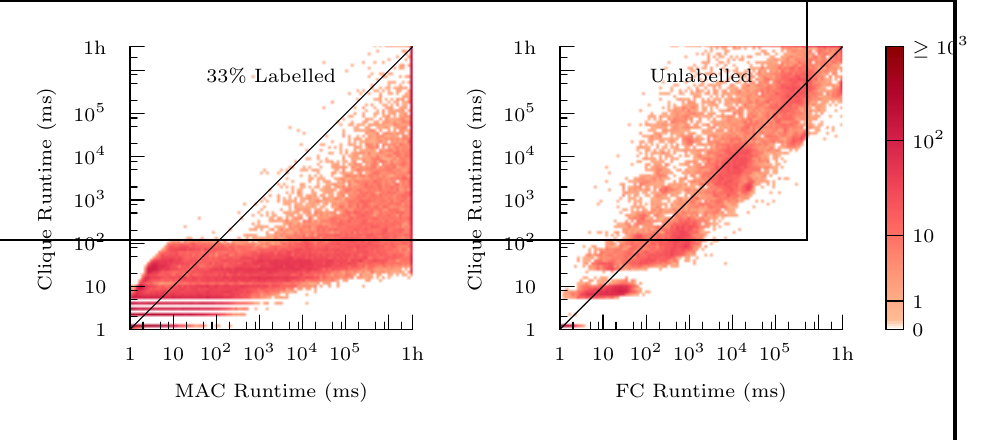
\begin{tikzpicture}[gnuplot]
%% generated with GNUPLOT 5.0p0 (Lua 5.2; terminal rev. 99, script rev. 100)
%% Tue 19 Apr 2016 13:37:01 AEST
\tikzset{every node/.append style={font={\scriptsize}}}
% \path (0.000,0.000) rectangle (10.922,7.366);
\gpcolor{color=gp lt color border}
\gpsetlinetype{gp lt border}
\gpsetdashtype{gp dt solid}
\gpsetlinewidth{1.00}
\draw[gp path] (1.320,5.785)--(1.320,2.197)--(4.908,2.197);
\node[gp node center,rotate=-270] at (0.246,3.991) {Clique Runtime (ms)};
\node[gp node center] at (3.114,1.427) {MAC Runtime (ms)};
\begin{scope}
\clip (1.320,5.785) rectangle (4.908,2.197);
\def\gprawrgbimagedata{%
  ffffffffffffffffffffffffffffffffffffffffffffffffffffffffffffffffffffffffffffffffffffffffffffffff%
  ffffffffffffffffffffffffffffffffffffffffffffffffffffffffffffffffffffffffffffffffffffffffffffffff%
  ffffffffffffffffffffffffffffffffffffffffffffffffffffffffffffffffffffffffffffffffffffffffffffffff%
  ffffffffffffffffffffffffffffffffffffffffffffffffffffffffffffffffffffffffffffffffffffffffffffffff%
  ffffffffffffffffffffffffffffffffffffffffffffffffffffffffffffffffffffffffffffffffffffffffffffffff%
  ffffffffffffffffffffffffffffffffffffffffffffac88ffffffffac88ffffffff9f7dff9f7dff9f7dffac88ff9f7d%
  ff9f7dffac88ff9576ff95768b0000ffffffffffffffffffffffffffffffffffffffffffffffffffffffffffffffffff%
  ffffffffffffffffffffffffffffffffffffffffffffffffffffffffffffffffffffffffffffffffffffffffffffffff%
  ffffffffffffffffffffffffffffffffffffffffffffffffffffffffffffffffffffffffffffffffffffffffffffffff%
  ffffffffffffffffffffffffffffffffffffffffffffffffffffffffffffffffffffffffffffffffffffffffffffffff%
  ffffffffffffffffffffffffffffffffffffffffffffffffffffffffffffffffffffffffffffffffffffffffffffffff%
  ffffffffffffffffffffffffffffffffffffffffffffffffffffffffffffffffffffffffffffffffffffffffffffffff%
  ffffffffffffffffffffffffffffffffffffffffffffffffffffffcf1d45ffffffffffffffffffffffffffffffffffff%
  ffffffffffffffffffffffffffffffffffffffffffffffffffffffffffffffffffffffffffffffffffffffffffffffff%
  ffffffffffffffffffffffffffffffffffffffffffffffffffffffffffffffffffffffffffffffffffffffffffffffff%
  ffffffffffffffffffffffffffffffffffffffffffffffffffffffffffffffffffffffffffffffffffffffffffffffff%
  ffffffffffffffffffffffffffffffffffffffffffffffffffffffffffffffffffffffffffffffffffffffffffffffff%
  ffffffffffffffffffffffffffffffffffffffffffffffffffffffffffffffffffffffffffffffffffffffffffffffff%
  ffffffffffffffac88ffffffffffffffffffffffffffffffffffffffffffffffffff9f7dffac88ffffffca1941ffffff%
  ffffffffffffffffffffffffffffffffffffffffffffffffffffffffffffffffffffffffffffffffffffffffffffffff%
  ffffffffffffffffffffffffffffffffffffffffffffffffffffffffffffffffffffffffffffffffffffffffffffffff%
  ffffffffffffffffffffffffffffffffffffffffffffffffffffffffffffffffffffffffffffffffffffffffffffffff%
  ffffffffffffffffffffffffffffffffffffffffffffffffffffffffffffffffffffffffffffffffffffffffffffffff%
  ffffffffffffffffffffffffffffffffffffffffffffffffffffffffffffffffffffffffffffffffffffffffffffffff%
  ffffffffffffffffffffffffffac88ffffffffffffffffffffffffffffffffffffffffffffffffffffffffffffffffff%
  ffffffffac88ffffffc7173effffffffffffffffffffffffffffffffffffffffffffffffffffffffffffffffffffffff%
  ffffffffffffffffffffffffffffffffffffffffffffffffffffffffffffffffffffffffffffffffffffffffffffffff%
  ffffffffffffffffffffffffffffffffffffffffffffffffffffffffffffffffffffffffffffffffffffffffffffffff%
  ffffffffffffffffffffffffffffffffffffffffffffffffffffffffffffffffffffffffffffffffffffffffffffffff%
  ffffffffffffffffffffffffffffffffffffffffffffffffffffffffffffffffffffffffffffffffffffffffffffffff%
  ffffffffffffffffffffffffffffffffffffffffffffffffffffffffffffffffffffffffffffffffffffffffffffffff%
  ffffffffffffffffffffac88ffffffffffffffffffffac88c7173effffffffffffffffffffffffffffffffffffffffff%
  ffffffffffffffffffffffffffffffffffffffffffffffffffffffffffffffffffffffffffffffffffffffffffffffff%
  ffffffffffffffffffffffffffffffffffffffffffffffffffffffffffffffffffffffffffffffffffffffffffffffff%
  ffffffffffffffffffffffffffffffffffffffffffffffffffffffffffffffffffffffffffffffffffffffffffffffff%
  ffffffffffffffffffffffffffffffffffffffffffffffffffffffffffffffffffffffffffffffffffffffffffffffff%
  ffffffffffffffffffffffffffffffffffffffffffffffffffffffffffffffffffffffffffffffffffffffffffffffff%
  ffffffffffffffffffffffffffffffffac88ffffffffffffffffffffffffffffffffac88ffffffc6163dffffffffffff%
  ffffffffffffffffffffffffffffffffffffffffffffffffffffffffffffffffffffffffffffffffffffffffffffffff%
  ffffffffffffffffffffffffffffffffffffffffffffffffffffffffffffffffffffffffffffffffffffffffffffffff%
  ffffffffffffffffffffffffffffffffffffffffffffffffffffffffffffffffffffffffffffffffffffffffffffffff%
  ffffffffffffffffffffffffffffffffffffffffffffffffffffffffffffffffffffffffffffffffffffffffffffffff%
  ffffffffffffffffffffac88ffffffffffffffffffffffffffffffffffffffffffffffffffffffffffffffffffffffff%
  ffffffffac88ffffffffffffffffffffac88ffffffffffffffac88ffffffffffffffffffffffffffffffffffffffffff%
  ffffffffffffc6163effffffffffffffffffffffffffffffffffffffffffffffffffffffffffffffffffffffffffffff%
  ffffffffffffffffffffffffffffffffffffffffffffffffffffffffffffffffffffffffffffffffffffffffffffffff%
  ffffffffffffffffffffffffffffffffffffffffffffffffffffffffffffffffffffffffffffffffffffffffffffffff%
  ffffffffffffffffffffffffffffffffffffffffffffffffffffffffffffffffffffffffffffffffffffffffffffffff%
  ffffffffffffffffffffffffffffffffffffffffffffffffffffffffffffffffffffffffffffffffffffffffffffffff%
  ffffffffffffffac88ffffffffffffffffffffffffffffffffffffffffffffffffffffffffffffffffffffffffffffff%
  ffffffffffffffffffffac88ff9576ffffffffac88c7173fffffffffffffffffffffffffffffffffffffffffffffffff%
  ffffffffffffffffffffffffffffffffffffffffffffffffffffffffffffffffffffffffffffffffffffffffffffffff%
  ffffffffffffffffffffffffffffffffffffffffffffffffffffffffffffffffffffffffffffffffffffffffffffffff%
  ffffffffffffffffffffffffffffffffffffffffffffffffffffffffffffffffffffffffffffffffffffffffffffffff%
  ffffffffffffffffffffffffffffffffffffffffffffffffffffffffffffffffffffffffffffffffffffffffffffffff%
  ffffffffffffffffffffffffffffffffffffffffffffffffffffffffffffffffffffffffffffffffac88ffffffffffff%
  ffffffffffffffffffffffffffffffffffffffac88ffffffff9f7dffac88ffffffffffffc1133affffffffffffffffff%
  ffffffffffffffffffffffffffffffffffffffffffffffffffffffffffffffffffffffffffffffffffffffffffffffff%
  ffffffffffffffffffffffffffffffffffffffffffffffffffffffffffffffffffffffffffffffffffffffffffffffff%
  ffffffffffffffffffffffffffffffffffffffffffffffffffffffffffffffffffffffffffffffffffffffffffffffff%
  ffffffffffffffffffffffffffffffffffffffffffffffffffffffffffffffffffffffffffffffffffffffffffffffff%
  ffffffffffffffffffffffffffffffffffffffffffffffffffffffffffffffac88ffffffffffffffffffffffffffffff%
  ffffffffffffffffffffffffffffffffffffffffffffffffffffffffffffffffffffffffffffffffffffffffffffffff%
  ffffffc8183fffffffffffffffffffffffffffffffffffffffffffffffffffffffffffffffffffffffffffffffffffff%
  ffffffffffffffffffffffffffffffffffffffffffffffffffffffffffffffffffffffffffffffffffffffffffffffff%
  ffffffffffffffffffffffffffffffffffffffffffffffffffffffffffffffffffffffffffffffffffffffffffffffff%
  ffffffffffffffffffffffffffffffffffffffffffffffffffffffffffffffffffffffffffffffffffffffffffffffff%
  ffffffffffffffffffffffffffffffffffffffffffffffffffffffffffffffffffffffffffffffffffffffffffffffff%
  ffffffffffffffffffffffffffffffffffffffffffffffffffac88ffffffffffffffac88ffac88ffffffffac88ffac88%
  ffffffffffffffffffffffffffffffffffffc8183fffffffffffffffffffffffffffffffffffffffffffffffffffffff%
  ffffffffffffffffffffffffffffffffffffffffffffffffffffffffffffffffffffffffffffffffffffffffffffffff%
  ffffffffffffffffffffffffffffffffffffffffffffffffffffffffffffffffffffffffffffffffffffffffffffffff%
  ffffffffffffffffffffac88ffffffffffffffffffffffffffffffffffffffffffffffffffffffffffffffffffffffff%
  ffffffffffffffffffffffffffffffffffffffffffffffffffffffffffffffffffffffffffffffffffffffffffffffff%
  ffffffffffffffffffffffffffffffffffffffffffffffffffffffffffffffffffffffffffac88ffffffffffffffffff%
  ffffffffac88ffac88ffffffffffffffffffffffffffac88ffffffffac88ff9f7dc6163effffffffffffffffffffffff%
  ffffffffffffffffffffffffffffffffffffffffffffffffffffffffffffffffffffffffffffffffffffffffffffffff%
  ffffffffffffffffffffffffffffffffffffffffffffffffffffffffffffffffffffffffffffffffffffffffffffffff%
  ffffffffffffffffffffffffffffffffffffffffffffffffffffffffffffffffffffffffffffffffffffffffffffffff%
  ffffffffffffffffffffffffffffffffffffffffffffffffffffffffffffffffffffffffffffffffffffffffffffffff%
  ffffffffffffffffffffffffffffffffffffffffffffffffffffffffffffffffffffffffffffffffffffffffffffffff%
  ffffffffffffffffffffffffffac88ffffffffffffffffffffffffffffffffffffffffffffffffffffffffffffffffff%
  c8183fffffffffffffffffffffffffffffffffffffffffffffffffffffffffffffffffffffffffffffffffffffffffff%
  ffffffffffffffffffffffffffffffffffffffffffffffffffffffffffffffffffffffffffffffffffffffffffffffff%
  ffffffffffffffffffffffffffffffffffffffffffffffffffffffffffffffffffffffffffffffffffffffffffffffff%
  ffffffffffffffffffffffffffffffffffffffffffffffffffffffffffffffffffffffffffffffffffffffffffffffff%
  ffffffffffffffffffffffffffffffffffffffffffffffffffffffffffffffffffffffffffffffffffffffffffffffff%
  ffffffffffffffffffffffffffffffffffffffffffffffffffffffffffffffffffffffffffffffffac88ffac88ffac88%
  ffffffffffffffac88ffffffffac88c4153cffffffffffffffffffffffffffffffffffffffffffffffffffffffffffff%
  ffffffffffffffffffffffffffffffffffffffffffffffffffffffffffffffffffffffffffffffffffffffffffffffff%
  ffffffffffffffffffffffffffffffffffffffffffffffffffffffffffffffffffffffffffffffffffffffffffffffff%
  ffffffffffffffffffffffffffffffffffffffffffffffffffffffffffffffffffffffffffffffffffffffffffffffff%
  ffffffffffffffffffffffffffffffffffffffffffffffffffffffffffffffffffffffffffffffffffffffffffffffff%
  ffffffffffffffffffffffffffffffffffffffffffffffffffffffffffffffffffffffffffac88ffffffffffffffffff%
  ffffffffffffffac88ffffffffffffffffffffac88ffffffffffffffffffc4143cffffffffffffffffffffffffffffff%
  ffffffffffffffffffffffffffffffffffffffffffffffffffffffffffffffffffffffffffffffffffffffffffffffff%
  ffffffffffffffffffffffffffffffffffffffffffffffffffffffffffffffffffffffffffffffffffffffffffffffff%
  ffffffffffffffffffffffffffffffffffffffffffffffffffffffffffffffffffffffffffffffffffffffffffffffff%
  ffffffffffffffffffffffffffffffffffffffffffffffffffffffffffffffffffffffffffffffffffffffffffffffff%
  ffffffffffffffffffffffffffffffffffffffffffffffffffffffffffffffffffffffffffffffffffffffffffffffff%
  ffffffffac88ffffffffffffffac88ffffffffac88ffac88ffffffffac88ffac88ff9f7dffac88ff9f7dffffffc3143b%
  ffffffffffffffffffffffffffffffffffffffffffffffffffffffffffffffffffffffffffffffffffffffffffffffff%
  ffffffffffffffffffffffffffffffffffffffffffffffffffffffffffffffffffffffffffffffffffffffffffffffff%
  ffffffffffffffffffffffffffffffffffffffffffffffffffffffffffffffffffffffffffffffffffffffffffffffff%
  ffffffffffffffffffffffffffffffffffffffffffffffffffffffffffffffffffffffffffffffffffffffffffffffff%
  ffffffffffffffffffffffffffffffffffffffffffffffffffffffffffffffffffffffffffffffffffffffffffffffff%
  ffffffffac88ffffffffac88ffffffffffffffffffffac88ffac88ffffffffac88ffffffffac88ffffffffffffff9f7d%
  ffac88ffffffffffffff9f7dc1133affffffffffffffffffffffffffffffffffffffffffffffffffffffffffffffffff%
  ffffffffffffffffffffffffffffffffffffffffffffffffffffffffffffffffffffffffffffffffffffffffffffffff%
  ffffffffffffffffffffffffffffffffffffffffffffffffffffffffffffffffffffffffffffffffffffffffffffffff%
  ffffffffffffffffffffffffffffffffffffffffffffffffffffffffffffffffffffffffffffffffffffffffffffffff%
  ffffffffffffffffffffffffffffffffffffffffffffffffffffffffffffffffffffffffffffffffffffffffffffffff%
  ffffffffffffffffffffac88ffffffffffffffffffffac88ffffffffffffffac88ffffffffffffffffffffac88ffffff%
  ffffffffac88ffac88ffffffffac88ffffffffffffffac88ffac88c4153cffffffffffffffffffffffffffffffffffff%
  ffffffffffffffffffffffffffffffffffffffffffffffffffffffffffffffffffffffffffffffffffffffffffffffff%
  ffffffffffffffffffffffffffffffffffffffffffffffffffffffffffffffffffffffffffffffffffffffffffffffff%
  ffffffffffffffffffffffffffffffffffffffffffffffffffffffffffffffffffffffffffffffffffffffffffffffff%
  ffffffffffffffffffffffffffffffffffffffffffffffffffffffffffffffffffffffffffffffffffffffffffffffff%
  ffffffffffffffffffffffffffffffffffffffffffffffffffffffffffffffffffffffffffffffffffffffffffffffff%
  ffffffffffffffffffff9576ffffffffffffffffffffffffffffffffffffffffffffac88ff9f7dffac88c2133affffff%
  ffffffffffffffffffffffffffffffffffffffffffffffffffffffffffffffffffffffffffffffffffffffffffffffff%
  ffffffffffffffffffffffffffffffffffffffffffffffffffffffffffffffffffffffffffffffffffffffffffffffff%
  ffffffffffffffffffffffffffffffffffffffffffffffffffffffffffffffffffffffffffffffffffffffffffffffff%
  ffffffffffffffffffffffffffffffffffffffffffffffffffffffffffffffffffffffffffffffffffffffffffffffff%
  ffffffffffffffffffffffffffffffffffffffffffffffffffffffffffffffffffffffffffffffffffffffffffffffff%
  ffac88ffffffffffffffffffffffffffffffffac88ffac88ffac88ffffffffac88ffffffffac88ffffffff9576ffac88%
  ff9576ffffffff9f7dc6163dffffffffffffffffffffffffffffffffffffffffffffffffffffffffffffffffffffffff%
  ffffffffffffffffffffffffffffffffffffffffffffffffffffffffffffffffffffffffffffffffffffffffffffffff%
  ffffffffffffffffffffffffffffffffffffffffffffffffffffffffffffffffffffffffffffffffffffffffffffffff%
  ffffffffffffffffffffffffffffffffffffffffffffffffffffffffffffffffffffffffffffffffffffffffffffffff%
  ffffffffffffffffffffffffffffffffffffffffffffffffffffffffffffffffffffffffff9f7dffffffffffffffffff%
  ffffffffffffffffffffffffffffffffffffffffffffffffffffffffffffffffffffffffffffffff9f7dffffffffffff%
  ffac88ffffffffac88ffac88ffffffffac88ffac88ff846ec01239ffffffffffffffffffffffffffffffffffffffffff%
  ffffffffffffffffffffffffffffffffffffffffffffffffffffffffffffffffffffffffffffffffffffffffffffffff%
  ffffffffffffffffffffffffffffffffffffffffffffffffffffffffffffffffffffffffffffffffffffffffffffffff%
  ffffffffffffffffffffffffffffffffffffffffffffffffffffffffffffffffffffffffffffffffffffffffffffffff%
  ffffffffffffffffffffffffffffffffffffffffffffffffffffffffffffffffffffffffffffffffffffffffffffffff%
  ffffffffffffffffffffffffffffffffffffffffffffffffffffffffffffffffffffffffffffffffac88ffffffff9f7d%
  ffffffffffffffffffffac88ffac88ffffffffac88ffffffff9576ffffffffac88ffac88ffffffc4153cffffffffffff%
  ffffffffffffffffffffffffffffffffffffffffffffffffffffffffffffffffffffffffffffffffffffffffffffffff%
  ffffffffffffffffffffffffffffffffffffffffffffffffffffffffffffffffffffffffffffffffffffffffffffffff%
  ffffffffffffffffffffffffffffffffffffffffffffffffffffffffffffffffffffffffffffffffffffffffffffffff%
  ffffffffffffffffffffffffffffffffffffffffffffffffffffffffffffffffffffffffffffffffffffffffffffffff%
  ffffffffffffffffffffac88ffffffffffffffffffffffffffffffffffffffffffffffffffffffffffffffac88ffffff%
  ffffffff9f7dffffffffffffffffffffac88ffffffffffffffffffffac88ff9f7dff9f7dffffffffffffffac88ff9f7d%
  ff9f7dffffffbd0f36ffffffffffffffffffffffffffffffffffffffffffffffffffffffffffffffffffffffffffffff%
  ffffffffffffffffffffffffffffffffffffffffffffffffffffffffffffffffffffffffffffffffffffffffffffffff%
  ffffffffffffffffffffffffffffffffffffffffffffffffffffffffffffffffffffffffffffffffffffffffffffffff%
  ffffffffffffffffffffffffffffffffffffffffffffffffffffffffffffffffffffffffffffffffffffffffffffffff%
  ffffffffffffffffffffffffffffffffffffffffffffffffffffffffffffffffffffffffffffffffffffffffffffffff%
  ffffffffffffffffffffffffffffffffffffffffffffac88ffffffffffffffffffffac88ffffffff9576ffffffffac88%
  ff9f7dffac88ff9576ff9f7dff9576ffffffffac88c2133affffffffffffffffffffffffffffffffffffffffffffffff%
  ffffffffffffffffffffffffffffffffffffffffffffffffffffffffffffffffffffffffffffffffffffffffffffffff%
  ffffffffffffffffffffffffffffffffffffffffffffffffffffffffffffffffffffffffffffffffffffffffffffffff%
  ffffffffffffffffffffffffffffffffffffffffffffffffffffffffffffffffffffffffffffffffffffffffffffffff%
  ffffffffffffffffffffffffffffffffffffffffffffffffffffffffffffffffffffffffffffffffffffffffffffffff%
  ffffffffffffffffffffffffffffffffffffffffffffffffff9f7dffffffffffffffac88ffffffffffffffffffffac88%
  ffac88ffffffff9f7dffffffffac88ffac88ff9576ffffffffac88ff9f7dff9576ffffffc1133affffffffffffffffff%
  ffffffffffffffffffffffffffffffffffffffffffffffffffffffffffffffffffffffffffffffffffffffffffffffff%
  ffffffffffffffffffffffffffffffffffffffffffffffffffffffffffffffffffffffffffffffffffffffffffffffff%
  ffffffffffffffffffffffffffffffffffffffffffffffffffffffffffffffffffffffffffffffffffffffffffffffff%
  ffffffffffffffffffffffffffffffffffffffffffffffffffffffffffffffffffffffffffffffffffffffffffffffff%
  ffffffffffffffffffffffffffffffffffffffffffffffffffffffffffffffffffffac88ffac88ffffffffffffffffff%
  ff9f7dffffffffffffffffffffac88ffffffffffffffac88ff9f7dff9576ffffffffac88ffffffff9f7dff9f7dff8c72%
  ff9f7dc01238ffffffffffffffffffffffffffffffffffffffffffffffffffffffffffffffffffffffffffffffffffff%
  ffffffffffffffffffffffffffffffffffffffffffffffffffffffffffffffffffffffffffffffffffffffffffffffff%
  ffffffffffffffffffffffffffffffffffffffffffffffffffffffffffffffffffffffffffffffffffffffffffffffff%
  ffffffffffffffffffffffffffffffffffffffffffffffffffffffffffffffffffffffffffffffffffffffffffffffff%
  ffffffffffffffffffffffffffffffffffffffffffffffffffffffffffffffffffffffffffffffffffffffac88ffffff%
  ffffffffffffffffffffffffffffffffffffff9f7dffac88ffac88ffffffffffffff9f7dffffffff9576ffac88ffac88%
  ffac88ff9f7dff9576ff846effac88ffac88c1133affffffffffffffffffffffffffffffffffffffffffffffffffffff%
  ffffffffffffffffffffffffffffffffffffffffffffffffffffffffffffffffffffffffffffffffffffffffffffffff%
  ffffffffffffffffffffffffffffffffffffffffffffffffffffffffffffffffffffffffffffffffffffffffffffffff%
  ffffffffffffffffffffffffffffffffffffffffffffffffffffffffffffffffffffffffffffffffffffffffffffffff%
  ffffffffffffffffffffffffffffffffffffffffffffffffffffffffffffffffffffffffffffffffffffffffffffffff%
  ffffffffac88ffffffffffffffffffffffffffac88ffffffffffffffffffffac88ff9f7dffffffffffffffac88ff9f7d%
  ffffffff9f7dff9576ff9f7dffac88ff9576ffac88ff9f7dff846eff8c72ff8c72c3143bffffffffffffffffffffffff%
  ffffffffffffffffffffffffffffffffffffffffffffffffffffffffffffffffffffffffffffffffffffffffffffffff%
  ffffffffffffffffffffffffffffffffffffffffffffffffffffffffffffffffffffffffffffffffffffffffffffffff%
  ffffffffffffffffffffffffffffffffffffffffffffffffffffffffffffffffffffffffffffffffffffffffffffffff%
  ffffffffffffffffffffffffffffffffffffffffffffffffffffffffffffffffffffffffffffffffffffffffffffffff%
  ffffffffffffffffffffffffffffffffffffffffffffac88ffffffffffffffac88ff9f7dffffffffac88ffac88ffac88%
  ffffffff9f7dff9f7dff9f7dff9f7dffac88ff9f7dffac88ffac88ffac88ff846eff9576ff9f7dff9f7dff9f7dff9576%
  c11239ffffffffffffffffffffffffffffffffffffffffffffffffffffffffffffffffffffffffffffffffffffffffff%
  ffffffffffffffffffffffffffffffffffffffffffffffffffffffffffffffffffffffffffffffffffffffffffffffff%
  ffffffffffffffffffffffffffffffffffffffffffffffffffffffffffffffffffffffffffffffffffffffffffffffff%
  ffffffffffffffffffffffffffffffffffffffffffffffffffffffffffffffac88ffffffffffffffffffffffffffffff%
  ffffffffffffffffffffffffffffffffffffffffffffffffffffffffffffffffffffffffffffffffffffffffffffffff%
  ffffffffac88ffac88ffffffffffffff9f7dffac88ffffffffffffffac88ffac88ffac88ff9576ffac88ffffffffac88%
  ff9576ff9576ff846eff846effffffbd1036ffffffffffffffffffffffffffffffffffffffffffffffffffffffffffff%
  ffffffffffffffffffffffffffffffffffffffffffffffffffffffffffffffffffffffffffffffffffffffffffffffff%
  ffffffffffffffffffffffffffffffffffffffffffffffffffffffffffffffffffffffffffffffffffffffffffffffff%
  ffffffffffffffffffffffffffffffffffffffffffffffffffffffffffffffffffffffffffffffffffffffffffffffff%
  ffffffffffffffac88ffffffffffffffffffffffffffffffffffffffffffffffffffffffffffffffffffffffffffffff%
  ffffffffffffffac88ffffffffffffffffffffac88ffac88ffac88ffac88ffac88ff9576ff846eff9f7dffffffff9f7d%
  ffffffffffffff9f7dffffffff9f7dffffffff9576ff9576ffac88ffac88c01239ffffffffffffffffffffffffffffff%
  ffffffffffffffffffffffffffffffffffffffffffffffffffffffffffffffffffffffffffffffffffffffffffffffff%
  ffffffffffffffffffffffffffffffffffffffffffffffffffffffffffffffffffffffffffffffffffffffffffffffff%
  ffffffffffffffffffffffffffffffffffffffffffffffffffffffffffffffffffffffffffffffffffffffffffffffff%
  ffffffffffffffffffffffffffffffffffffffffffffffffffffffffac88ffffffffffffffffffffffffffffffffffff%
  ffffffffffffffffffffffffffffffffffffffffffffac88ffffffffffffffffffffffffffffffffffffffffffff9576%
  ffac88ffac88ff9f7dff846effffffffac88ff846eff9576ff9576ffac88ff8c72ff9f7dff8c72ffffffff9f7dbf1138%
  ffffffffffffffffffffffffffffffffffffffffffffffffffffffffffffffffffffffffffffffffffffffffffffffff%
  ffffffffffffffffffffffffffffffffffffffffffffffffffffffffffffffffffffffffffffffffffffffffffffffff%
  ffffffffffffffffffffffffffffffffffffffffffffffffffffffffffffffffffffffffffffffffffffffffffffffff%
  ffffffffffffffffffffffffffffffffffffffffffffffffffffffffffffffffffffffffffffffffffffffffffffffff%
  ffffffffffffffffffffffffffffffffffffffac88ffffffffffffffffffffffffffffffff9576ffffffffac88ffffff%
  ffffffffac88ffffffffac88ffffffff9576ff9f7dffac88ff8c72ff9576ff8c72ffac88ffac88ff9f7dff9f7dffac88%
  ffffffff8c72ff846effac88c11239ffffffffffffffffffffffffffffffffffffffffffffffffffffffffffffffffff%
  ffffffffffffffffffffffffffffffffffffffffffffffffffffffffffffffffffffffffffffffffffffffffffffffff%
  ffffffffffffffffffffffffffffffffffffffffffffffffffffffffffffffffffffffffffffffffffffffffffffffff%
  ffffffffffffffffffffffffffffffffffffffffffffffffffffffffffffffffffffffffffffffffffffffffffffffff%
  ffffffffffffffffffffffffffffffffffffffffffffffffffffffffffffffffffffffffffffffffffffffffffffffff%
  ffffffffffffffffffffac88ffffffff9f7dff9f7dffac88ffffffff9f7dff9f7dffac88ffac88ff8c72ff9f7dff9f7d%
  ff8c72ff9576ff8c72ff9f7dff8c72ff9f7dff846eff8c72ff7e6cc11239ffffffffffffffffffffffffffffffffffff%
  ffffffffffffffffffffffffffffffffffffffffffffffffffffffffffffffffffffffffffffffffffffffffffffffff%
  ffffffffffffffffffffffffffffffffffffffffffffffffffffffffffffffffffffffffffffffffffffffffffffffff%
  ffffffffffffffffffffffffffffffffffffffffffffffffffffffffffffffffffffffffffffffffffffffffffffffff%
  ffffffffffffffffffffffffffffffffffffffffffffffffffffffffffffffffffffffffffffffffffffffffffffffff%
  ffffffffffffffac88ffffffffffffffffffffffffffffffffac88ffffffffac88ffffffffac88ffac88ff9f7dffac88%
  ffac88ffac88ff9f7dff7e6cffac88ff9f7dffffffff9576ff9f7dff9576ff9f7dff9576ffac88fb605fc2133bffffff%
  ffffffffffffffffffffffffffffffffffffffffffffffffffffffffffffffffffffffffffffffffffffffffffffffff%
  ffffffffffffffffffffffffffffffffffffffffffffffffffffffffffffffffffffffffffffffffffffffffffffffff%
  ffffffffffffffffffffffffffffffffffffffffffffffffffffffffffffffffffffffffffffffffffffffffffffffff%
  ffffffffffffffffffffffffffffffffffffffffffffffffffffffffffffffffffffffffffac88ffffffffffffffffff%
  ffffffffffffffffffffac88ffac88ffffffffffffffffffffffffffffffffac88ffffffffffffff9f7dffac88ffac88%
  ffffffffac88ffffffff846eff846eff9576ffac88ff846effffffff8c72ff9576ff9f7dff9576ff846effac88ff7869%
  ff7e6cff9576ff8c72c4153cffffffffffffffffffffffffffffffffffffffffffffffffffffffffffffffffffffffff%
  ffffffffffffffffffffffffffffffffffffffffffffffffffffffffffffffffffffffffffffffffffffffffffffffff%
  ffffffffffffffffffffffffffffffffffffffffffffffffffffffffffffffffffffffffffffffffffffffffffffffff%
  ffffffffffffffffffffffffffffffffffffffffffffffffffffffffffffffffffffffffffffffffffffffffffffffff%
  ffffffffffffffffffffffffffffffffffffffffffffffffffffffffffffffffffffac88ffffffffac88ffffffffac88%
  ffffffffffffffffffffffffff9f7dff9f7dffac88ffffffffac88ff846eff846eff9576ff7869ffffffff8c72ffffff%
  ff8c72ffac88ff8c72ff7e6cff9576ff8c72ff846eff9576c01239ffffffffffffffffffffffffffffffffffffffffff%
  ffffffffffffffffffffffffffffffffffffffffffffffffffffffffffffffffffffffffffffffffffffffffffffffff%
  ffffffffffffffffffffffffffffffffffffffffffffffffffffffffffffffffffffffffffffffffffffffffffffffff%
  ffffffffffffffffffffffffffffffffffffffffffffffffffffffffffffffffffffffffffffffffffffffffffffffff%
  ffffffffffffffffffffffffffffffffffffffffffffffffffac88ffffffffffffffffffffffffff9f7dffffffffffff%
  ffffffffffffffffffffffffffac88ffffffffac88ffffffffffffff9f7dffffffffac88ffac88ff9f7dffac88ff9576%
  ffac88ffffffff846eff9f7dff8c72ff846eff7e6cff9f7dff7869ff9576ff7e6cff8c72ff7e6cc1133affffffffffff%
  ffffffffffffffffffffffffffffffffffffffffffffffffffffffffffffffffffffffffffffffffffffffffffffffff%
  ffffffffffffffffffffffffffffffffffffffffffffffffffffffffffffffffffffffffffffffffffffffffffffffff%
  ffffffffffffffffffffffffffffffffffffffffffffffffffffffffffffffffffffffffffffffffffffffffffffffff%
  ffffffffffffffffffffffffffffffffffffffffffffffffffffffffffffffffffffffffffffffffffffffffffffffff%
  ffffffffffffffffffffffffffffffffac88ffac88ffffffffffffffac88ffffffff9f7dffffffffac88ff9f7dff9576%
  ff8c72ff9576ffac88ff7e6cffac88ff9f7dffac88ff846eff8c72ff9f7dff9576ff9576ff7367ff6f65ff846eff8c72%
  ff7e6cff7e6cc3143bffffffffffffffffffffffffffffffffffffffffffffffffffffffffffffffffffffffffffffff%
  ffffffffffffffffffffffffffffffffffffffffffffffffffffffffffffffffffffffffffffffffffffffffffffffff%
  ffffffffffffffffffffffffffffffffffffffffffffffffffffffffffffffffffffffffffffffffffffffffffffffff%
  ffffffffffffffffffffffffffffffffffffffffffffffffffffffffffffffffffffffffffffffffffffffffffffffff%
  ffffffffffffffffffffffffffffffffffffffac88ffffffffffffffffffffffffffffffffffffffffffffffffffac88%
  ffffffffac88ffac88ff9576ffac88ffffffffac88ffac88ff9576ff9f7dffac88ff7869ffac88ff9f7dff8c72ff7869%
  ff8c72ff9f7dff7367ff7e6cff9576ff6f65ff7e6cc6163dffffffffffffffffffffffffffffffffffffffffffffffff%
  ffffffffffffffffffffffffffffffffffffffffffffffffffffffffffffffffffffffffffffffffffffffffffffffff%
  ffffffffffffffffffffffffffffffffffffffffffffffffffffffffffffffffffffffffffffffffffffffffffffffff%
  ffffffffffffffffffffffffffffffffffffffffffffffffffffffffffffffffffffffffffffffffffffffffffffffff%
  ffffffffffffffffffffffffffffffffffffffffffffac88ffac88ffffffffffffffac88ffffffffffffffac88ffffff%
  ffffffffffffffffffffffffff9576ffffffffffffff9f7dffac88ff9f7dffac88ff9576ff9f7dffac88ff846eff7e6c%
  ff7869ff846effac88ffac88ffac88ff9f7dff7e6cffac88ff846eff7869ff8c72ff8c72c4153cffffffffffffffffff%
  ffffffffffffffffffffffffffffffffffffffffffffffffffffffffffffffffffffffffffffffffffffffffffffffff%
  ffffffffffffffffffffffffffffffffffffffffffffffffffffffffffffffffffffffffffffffffffffffffffffffff%
  ffffffffffffffffffffffffffffffffffffffffffffffffffffffffffffffffffffffffffffffffffffffffffffffff%
  ffffffffffffffffffffffffffffffffffffffffffffffffffac88ffffffffffffffffffffffffffffffffffffffffff%
  ffffffffac88ffffffffac88ffac88ffac88ffffffffac88ffffffffac88ffac88ffffffffac88ff8c72ffffffffffff%
  ff8c72ff9f7dff9f7dff9576ff7869ff9f7dff7e6cff7869ff8c72ffac88ff7869ffac88ff8c72ff8c72ff7869ff7e6c%
  ff9576c4153cffffffffffffffffffffffffffffffffffffffffffffffffffffffffffffffffffffffffffffffffffff%
  ffffffffffffffffffffffffffffffffffffffffffffffffffffffffffffffffffffffffffffffffffffffffffffffff%
  ffffffffffffffffffffffffffffffffffffffffffffffffffffffffffffffffffffffffffffffffffffffffffffffff%
  ffffffffffffffffffffffffffffffffffffffffffffffffffffffffffffffffffffffffffffffffffffffffffffffff%
  ffffffffffffffffffffffffffffffffac88ffffffffffffffffffffffffffac88ff9f7dff9f7dffffffffac88ffffff%
  ff9f7dffac88ff8c72ff8c72ff9576ffffffff9f7dffac88ff846eff7869ff9576ffffffff846eff9576ff8c72ff7869%
  ff846eff9576ff7e6cff6b63ff7e6cff8c72cb1a41ffffffffffffffffffffffffffffffffffffffffffffffffffffff%
  ffffffffffffffffffffffffffffffffffffffffffffffffffffffffffffffffffffffffffffffffffffffffffffffff%
  ffffffffffffffffffffffffffffffffffffffffffffffffffffffffffffffffffffffffffffffffffffffffffffffff%
  ffffffffffffffffffffffffffffffffffffffffffffffffffffffffffffffffffffffffffffffffffffffffffffffff%
  ffac88ffac88ffffffffffffffffffffac88ffffffffac88ffffffffffffffffffffac88ffffffffffffffffffffac88%
  ff9f7dff9f7dff9f7dff9576ffac88ffffffff8c72ff9f7dffac88ff8c72ff9f7dff8c72ff9576ff7e6cff7869ffac88%
  ff8c72ff9576ff7869ff846eff7e6cff6b63ffac88ff9576ff846eff9576ff8c72c8183fffffffffffffffffffffffff%
  ffffffffffffffffffffffffffffffffffffffffffffffffffffffffffffffffffffffffffffffffffffffffffffffff%
  ffffffffffffffffffffffffffffffffffffffffffffffffffffffffffffffffffffffffffffffffffffffffffffffff%
  ffffffffffffffffffffffffffffffffffffffffffffffffffffffffffffffffffffffffffac88ffffffffffffffffff%
  ffffffffffffffac88ffffffffac88ffffffffffffffffffffffffffac88ffac88ffac88ffffffffac88ff9f7dffac88%
  ffffffffffffffffffffffffffffffffac88ffac88ffffffff846effffffffffffffac88ff9f7dff7869ff8c72ff8c72%
  ff9576ff8c72ff846eff9576ff7e6cff846eff846eff7e6cff7367ff7e6cff9576ff7e6cff8c72ff9f7dff9f7dff7e6c%
  c8183fffffffffffffffffffffffffffffffffffffffffffffffffffffffffffffffffffffffffffffffffffffffffff%
  ffffffffffffffffffffffffffffffffffffffffffffffffffffffffffffffffffffffffffffffffffffffffffffffff%
  ffffffffffffffffffffffffffffffffffffffffffffffffffffffffffffffffffffffffffffffffffffffffffffffff%
  ffac88ffffffffac88ffffffffffffffffffffac88ffffffffffffff9f7dffffffffffffffffffffffffffffffffffff%
  ffffffffffffffffffffffffffac88ffffffffffffffffffffffffff9f7dff9f7dffffffffac88ff9576ffac88ffac88%
  ff9f7dffffffffac88ff846effffffffac88ff9f7dff846eff6f65ff7367ff846eff9576ff8c72ff846eff846eff7e6c%
  ff9576ff846eff8c72ff8c72ff6b63c8183fffffffffffffffffffffffffffffffffffffffffffffffffffffffffffff%
  ffffffffffffffffffffffffffffffffffffffffffffffffffffffffffffffffffffffffffffffffffffffffffffffff%
  ffffffffffffffffffffffffffffffffffffffffffffffffffffffffffffffffffffffffffffffffffffffffffffffff%
  ffffffffffffffffffffffffffffffffffffffffffffffffffffffffffffffffffffffffffffffffffffffffffffffff%
  ffffffffffffffffffffac88ffffffffffffffac88ffffffffac88ffffffffac88ffffffffffffffffffffac88ffffff%
  ffffffffffffffac88ff7e6cff846eff9576ff846eff9f7dff846eff7e6cff9f7dff7e6cff7869ff8c72ff7e6cff9f7d%
  ff846eff8c72ff9f7dffac88ff9576ff846eff8c72ff7367ff846effac88c7173effffffffffffffffffffffffffffff%
  ffffffffffffffffffffffffffffffffffffffffffffffffffffffffffffffffffffffffffffffffffffffffffffffff%
  ffffffffffffffffffffffffffffffffffffffffffffffffffffffffffffffffffffffffffffffffffffffffffffffff%
  ffffffffffffffffffffffffffffffffffffffffffffffffffffffffffffffffffffffffffffffffffffffffffffffff%
  ffffffffffffffffffffac88ffffffffffffffffffffffffffffffffffffffffffffac88ffac88ffffffffac88ffac88%
  ffac88ffffffffffffffffffffac88ffac88ff9576ff9576ffac88ffac88ff9576ff9576ffac88ff9f7dff9576ff9576%
  ff9576ff7e6cff9576ff7e6cff7e6cff846eff8c72ff9576ff7869ff8c72ff7869ff7e6cfd6561fe6862ff7e6cc6163e%
  ffffffffffffffffffffffffffffffffffffffffffffffffffffffffffffffffffffffffffffffffffffffffffffffff%
  ffffffffffffffffffffffffffffffffffffffffffffffffffffffffffffffffffffffffffffffffffffffffffffffff%
  ffffffffffffffffffffffffffffffffffffffffffffffffffffffffffffffffffffffffffffffffffffffffffffffff%
  ffffffffffffffffffffffffffffffffffffffffffffffffffffffffffffffac88ffffffffffffffffffffffffffffff%
  ff9f7dffffffffffffffac88ffffffffac88ff9f7dffac88ffffffffffffffac88ffac88ff8c72ffac88ff846effac88%
  ff846eff7e6cff8c72ff7e6cff7e6cff846eff8c72fd6561ff7869ff7869ff9576ff7e6cff9576ff8c72ff7e6cffffff%
  ff9576ff7869ff8c72ff7367c8183fffffffffffffffffffffffffffffffffffffffffffffffffffffffffffffffffff%
  ffffffffffffffffffffffffffffffffffffffffffffffffffffffffffffffffffffffffffffffffffffffffffffffff%
  ffffffffffffffffffffffffffffffffffffffffffffffffffffffffffffffffffffffffffffffffffffffffffffffff%
  ffffffffffffffffffffffffffffffffffffffffffffffffffffffffffffffac88ffffffffac88ffffffffffffffffff%
  ffffffffffffff9f7dffac88ffffffffffffffffffffffffffac88ffffffffffffffac88ffac88ff9f7dff8c72ffac88%
  ffac88ff9f7dffffffff7e6cff9f7dffac88ff9576ff846eff7e6cfe6862ff846eff7869ff8c72ff6f65ff7367ff9576%
  ff7869ff846eff9f7dff7e6cfc6260ff9f7dff7869ff8c72ff7869cc1a42ffffffffffffffffffffffffffffffffffff%
  ffffffffffffffffffffffffffffffffffffffffffffffffffffffffffffffffffffffffffffffffffffffffffffffff%
  ffffffffffffffffffffffffffffffffffffffffffffffffffffffffffffffffffffffffffffffffffffffffffffffff%
  ffffffffffffffffffffffffffffffffffffffffffffffffffffffffffffffffffffffffffffffffffffffffffffffff%
  ffac88ffffffffac88ffffffffac88ffffffffffffffac88ffac88ffffffffac88ffffffffac88ff9f7dffffffffac88%
  ff9f7dff9f7dffffffffac88ff8c72ff9f7dff846effac88ff846eff9f7dff846eff9576ff8c72ff7e6cff6f65ff7869%
  ff7367ff846eff7869fe6862ff9576ff7869ff7e6cff6b63ff7e6cff7e6cff9576ff846eff7869ff846ec8183fffffff%
  ffffffffffffffffffffffffffffffffffffffffffffffffffffffffffffffffffffffffffffffffffffffffffffffff%
  ffffffffffffffffffffffffffffffffffffffffffffffffffffffffffffffffffffffffffffffffffffffffffffffff%
  ffffffffffffffffffffffffffffffffffffffffffffffffffffffffffffffffffffffffffffffffffffffffffffffff%
  ffffffffac88ffffffffffffffffffffffffffffffffffffffffffffac88ffffffffac88ffac88ffffffffffffffffff%
  ff9f7dffffffffffffffac88ffac88ff9f7dff9f7dff9576ffac88ffffffffac88ff8c72ff7869ff7869ff8c72ff9576%
  ff7367ff7869ff8c72ff8c72ff7367ff846eff7869ff846eff6f65ff846eff846eff7e6cff7869ff8c72fd6561ff9f7d%
  ff9576ff846eff9f7dcb1a41ffffffffffffffffffffffffffffffffffffffffffffffffffffffffffffffffffffffff%
  ffffffffffffffffffffffffffffffffffffffffffffffffffffffffffffffffffffffffffffffffffffffffffffffff%
  ffffffffffffffffffffffffffffffffffffffffffffffffffffffffffffffffffffffffffffffffffffffffffffffff%
  ffffffffffffffffffffffffffffffffffffffffffffffffffffffffffffffffffffffffffac88ffffffffac88ffffff%
  ff8c72ffac88ffffffffffffffffffffac88ffac88ffffffffffffffac88ffac88ff9f7dffac88ffffffffac88ff8c72%
  ff9576ff8c72ff9576ff9576ff7e6cff9f7dff6f65ff7869ff6b63ff7869ff7869ff846effac88ff846eff7367ff7e6c%
  ff6b63ff7869ff6f65ff8c72ff846eff846eff6b63fe6862ca1940ffffffffffffffffffffffffffffffffffffffffff%
  ffffffffffffffffffffffffffffffffffffffffffffffffffffffffffffffffffffffffffffffffffffffffffffffff%
  ffffffffffffffffffffffffffffffffffffffffffffffffffffffffffffffffffffffffffffffffffffffffffffffff%
  ffffffffffffffffffffffffffffffffffffffffffffffffffffffffffffffffffff9f7dffffffffffffff9f7dffffff%
  ffffffffffffffac88ffffffffffffffac88ff9f7dffffffffac88ff9f7dffac88ff9576ffffffff9f7dff9f7dffffff%
  ffac88ff9f7dffffffff9f7dff9576ff846effffffff8c72ff8c72ff9576ff6f65ff7e6cff6b63ff7e6cff846efe6862%
  ff6f65ff8c72ff6b63ff846eff7869ff8c72ff7869ff9576ff7869ff7869fe6862ff6f65ff6f65d42148ffffffffffff%
  ffffffffffffffffffffffffffffffffffffffffffffffffffffffffffffffffffffffffffffffffffffffffffffffff%
  ffffffffffffffffffffffffffffffffffffffffffffffffffffffffffffffffffffffffffffffffffffffffffffffff%
  ffffffffffffffffffffffffffffffffffffffffffffffffffffffffffffffffffffffffffffffffffffffac88ffffff%
  ffffffffffffffffffffac88ffffffffac88ffffffffac88ffffffff9f7dffffffffac88ffac88ff9f7dff9576ffac88%
  ffac88ffac88ffffffff8c72ff9f7dff9f7dffac88ff8c72ff8c72ff9f7dffac88ff846eff9576ff8c72ff7e6cff7367%
  ff7367ff7e6cff7e6cff6f65ff7e6cff7367ff7869ff7e6cff7869ff8c72ff7367ff846eff8c72ff7869ff7e6cff7367%
  ff6b63ff9576d11e46ffffffffffffffffffffffffffffffffffffffffffffffffffffffffffffffffffffffffffffff%
  ffffffffffffffffffffffffffffffffffffffffffffffffffffffffffffffffffffffffffffffffffffffffffffffff%
  ffffffffffffffffffffffffffffffffffffffffffffffffffffffffffffffffffffffffffffffffffffffffffffffff%
  ffffffffffffffac88ffffffffac88ffffffffffffffffffff9f7dffffffffac88ffac88ffac88ffac88ffac88ffffff%
  ffac88ffac88ffffffff9f7dffac88ff9576ff846eff9f7dffac88ff9f7dffac88ff9f7dff9f7dffac88ff9f7dff9f7d%
  ff8c72ff7869ff7869ff7e6cff846efd6561fd6561ff6f65fe6862ff7869ff7367ff8c72ff7869ff7367ff7869ff8c72%
  fe6862ff8c72ff846eff7367ff6b63ff846eff7e6cd11e46ffffffffffffffffffffffffffffffffffffffffffffffff%
  ffffffffffffffffffffffffffffffffffffffffffffffffffffffffffffffffffffffffffffffffffffffffffffffff%
  ffffffffffffffffffffffffffffffffffffffffffffffffffffffffffffffffffffffffffffffffffffffffffffffff%
  ffffffffac88ffffffffffffffffffffac88ffffffffffffffffffffffffffffffffffffffffffffffffffffffffac88%
  ffac88ffac88ffffffffac88ffac88ffac88ffffffffac88ffac88ff9f7dffac88ffac88ffffffffac88ff9576ffffff%
  ff9f7dff8c72ff9f7dff8c72ff8c72ff9f7dff7869ff7e6cff846eff6b63ff846eff6b63fb605fff7e6cff9576ff8c72%
  ff7869ff7869ff7e6cff846eff6f65ff7869ff7869ff6b63ff6f65ff9f7dff7367ff846ed21f47ffffffffffffffffff%
  ffffffffffffffffffffffffffffffffffffffffffffffffffffffffffffffffffffffffffffffffffffffffffffffff%
  ffffffffffffffffffffffffffffffffffffffffffffffffffffffffffffffffffffffffffffffffffffffffffffffff%
  ffffffffffffffffffffffffffffffffffffffffffffffffffffffffffffffffffffffffffffffffac88ffffffffffff%
  ffffffffffffffffffffffffffffffffffffffac88ffffffff9576ffac88ffac88ffac88ffac88ffac88ff9f7dffac88%
  ffffffffac88ffac88ffffffffffffff9f7dffac88ff9576ff6b63ff7e6cff9f7dff7869ff7e6cff9576fe6862ff846e%
  fd6561ff6b63ff6f65ff846efe6862ff6b63ff9576ff6b63fd6561ff846eff9576ff8c72ff846eff8c72ff7e6cff7869%
  ff7869cd1c43ffffffffffffffffffffffffffffffffffffffffffffffffffffffffffffffffffffffffffffffffffff%
  ffffffffffffffffffffffffffffffffffffffffffffffffffffffffffffffffffffffffffffffffffffffffffffffff%
  ffffffffffffffffffffffffffffffffffffffffffffffffffffffffffffffffffffffffffffffffffffffffffffffff%
  ffffffffac88ffffffffffffffffffffffffffffffffffffffac88ffffffffffffffac88ffffffffac88ff9576ff9f7d%
  ff9f7dff9576ffac88ffffffffac88ff9576ffac88ffffffff9f7dffffffffffffff8c72ff9576ff9576ff846eff7869%
  ff9576ff9576ff6f65ff7e6cff6f65ff7367ff846eff7869ff6f65ff846eff7869ff6f65ff8c72ff9f7dff6f65ff7367%
  ff6f65ff6f65ff8c72ff9f7dff7e6cff846ed01e45ffffffffffffffffffffffffffffffffffffffffffffffffffffff%
  ffffffffffffffffffffffffffffffffffffffffffffffffffffffffffffffffffffffffffffffffffffffffffffffff%
  ffffffffffffffffffffffffffffffffffffffffffffffffffffffffffffffffffffffffffffffffffffffac88ffffff%
  ffffffffffffffffffffffffffffffffac88ffffffffffffffac88ffffffffac88ffffffffffffffffffffac88ff9f7d%
  ffac88ffac88ff9f7dffac88ffffffff9f7dff9f7dff8c72ffffffff7e6cff9576ff8c72ffac88ff9f7dff9576ff9576%
  ff8c72ffffffff9f7dff846eff6b63fe6862ff7e6cfa5e5ffd6561ff6f65ff7869fd6561ff6f65ff6f65ff9576ff9576%
  ff6f65ff846eff7367ff846eff6f65ff7e6cfd6561ff6f65fd6561ff846eff7e6cd52248ffffffffffffffffffffffff%
  ffffffffffffffffffffffffffffffffffffffffffffffffffffffffffffffffffffffffffffffffffffffffffffffff%
  ffffffffffffffffffffffffffffffffffffffffffffffffffffffffffffffffffffffffffffffffffffffffffffffff%
  ffffffffffffffffffffffffffffffffffffffffffffffffffac88ffffffffffffffac88ffffffffac88ffffffffac88%
  ffac88ffffffffffffffffffffac88ffac88ff9f7dffffffffac88ff9f7dffffffffac88ff9f7dffac88ff9576ffac88%
  ff8c72ff9f7dff9576ffac88ff9f7dff846eff8c72ff846eff7367ff7e6cff6f65ff8c72ff846eff6b63fe6862f95c5e%
  ff7367ff6f65ff846eff9f7dff7e6cff6f65ff7e6cff7869fe6862ff7e6cff7869ff9f7dfe6862ff846eff846eff7e6c%
  d72549ffffffffffffffffffffffffffffffffffffffffffffffffffffffffffffffffffffffffffffffffffffffffff%
  ffffffffffffffffffffffffffffffffffffffffffffffffffffffffffffffac88ffffffffffffffffffffffffffffff%
  ffffffffffffffffffffffffffffffffffffffffffffffffffffffffac88ffffffffffffffffffffffffffffffffffff%
  ffffffffffffffffffffac88ffac88ffffffff9576ffac88ffffffff9576ffffffffac88ff8c72ff9576ff846effffff%
  ffffffff6f65ffac88ffffffff9f7dff9576ff9f7dff9f7dff846eff6f65ff7367ff7869ff846eff846eff8c72ff7367%
  fc6260ff7e6cfe6862ff6f65ff6b63ff6f65ff7367ff6b63fe6862ff6b63ff846eff6f65ff7869ff7869ff7367ff7869%
  ff7869ff6f65ff7e6cff7367fe6862d72549ffffffffffffffffffffffffffffffffffffffffffffffffffffffffffff%
  ffffffffffffffffffffffffffffffffffffffffffffffffffffffffffffffffffffffffffffffffffffffffffffffff%
  ffffffffffffffffffffffffffffffffffffffffffffffffffffffffffffffffffffffffffffffffffffffffffffffff%
  ffffffffffffffffffffffffffac88ffffffffffffffffffffac88ff9f7dffac88ffac88ffac88ff9f7dff7e6cffac88%
  ff9f7dffac88ffac88ffffffff6f65ff9576ff7367ffac88ff846effac88ff846eff7e6cff7e6cff7e6cff6f65ff7367%
  ff8c72fe6862ff7869ff7869fb605fff7e6cff6f65ff7367ff7367fc6260fc6260ff846eff7869ff7367ff7869ff7367%
  ff846efd6561ff7869ff846eff6b63ff7367ff7869ff7367ff846eff7367d62449ffffffffffffffffffffffffffffff%
  ffffffffffffffffffffffffffffffffffffffffffffffffffffffffffffffffffffffffffffffffffffffffffffffff%
  ffffffffffffffffffffffffffffffffffffffffffffffffffffffffffffffffffffffffffffffffffffffffffffffff%
  ffffffffffffffffffffffffffffffffffffffffffff9f7dffffffffac88ffffffffffffffffffffffffffffffffffff%
  ffffffffffffffac88ff9f7dff8c72ff9f7dffac88ff8c72ffac88ff9576ff8c72ff9576ff8c72ff9576ff9576ff8c72%
  ff9f7dff9576ff8c72ff7869ff7869ff6b63fd6561ff6b63ff7367ff7367ff7869ff7367ff7869fe6862fb605fff6b63%
  ff6b63fd6561ff7869fe6862ff7367ff6f65ff6f65ff7367fe6862ff6b63ff6f65fe6862ff9576ff9f7dff7e6cd62449%
  ffffffffffffffffffffffffffffffffffffffffffffffffffffffffffffffffffffffffffffffffffffffffffffffff%
  ffffffffffffffffffffffffffac88ffffffffffffffffffffffffffffffffffffffffffffffffffffffffffffffffff%
  ffffffffffffffffffffffffffffffffffffffffffffffffffffffffffffffffffffffffffffffffac88ffac88ff9f7d%
  ffac88ffac88ffffffffffffffac88ffac88ffac88ffac88ffffffff846eff9f7dff8c72ff8c72ff9576ff7869ff8c72%
  ff7367ff9f7dff8c72ff7367ff6b63ff846eff6f65ff9576ff7e6cff8c72ff7367ff6f65ff7e6cff6f65ff6b63ff6b63%
  ff6f65fe6862fd6561ff7869fe6862ff6f65f7585dfb605ffb605fff6f65ff7367fd6561ff6f65ff6f65ff7367ff8c72%
  ff7367ff9f7dff7e6cff8c72db2a4cffffffffffffffffffffffffffffffffffffffffffffffffffffffffffffffffff%
  ffffffffffffffffffffffffffffffffffffffffffffffffffffffffffffffffffffffffffffffffffffffffffffffff%
  ffffffffffffffffffffffffffffffffffffffffffffffffffffffffac88ffffffffffffffffffffffffffffffffffff%
  ffac88ffac88ff9f7dffffffffac88ffffffffffffffac88ff8c72ffffffffac88ff7e6cffac88ff8c72ff9f7dff8c72%
  ffac88ff8c72ff7367ff9576ff9576ff846eff9f7dff8c72ff6b63ff846efd6561ff846efe6862ff7869fc6260ff6f65%
  ff7869ff6f65ff6f65ff6b63ff6f65fb605ffc6260ff7367fd6561f95c5eff6f65ff7367ff7367ff7367ff6f65fb605f%
  f6545cff7869ff7869ff6b63ff6b63fc6260fc6260ff8c72ff7367db2a4cffffffffffffffffffffffffffffffffffff%
  ffffffffffffffffffffffffffffffffffffffffffffffffffffffffffffffffffffffffffffffffffffffffffffffff%
  ffffffffffffffffffffffffffffffffffffffffffffffffffac88ffffffffffffffffffffffffffffffffffffffffff%
  ffffffffffffffffffffffffffffffffffffffffffffffffffffffffffffffffffff9f7dffffffffffffff9576ff9f7d%
  ffac88ff846effac88ffac88ffac88ff7e6cff9f7dff7869ff846eff8c72ff846eff7367ff8c72ff7869ff7e6cff7869%
  ff7e6cff8c72ff9f7dff7e6cff8c72ff6b63ff6f65fe6862ff7367fa5e5fff846efc6260ff7869ff6b63ff6b63ff7367%
  fe6862ff7869ff6b63fe6862f95c5ef95c5eff7869ff6b63fe6862ff6f65fe6862ff7869ff846eff7e6cda294bffffff%
  ffffffffffffffffffffffffffffffffffffffffffffffffffffffffffffffffffffffffffffffffffffffffffffffff%
  ffffffffffffffffffffffffffffffffffffffffffffffffffffffffffffffffffffffffffffffffffffffffffffffff%
  ffffffffffffffffffffffffffffffffffffffffffffffffffac88ff9f7dffac88ffac88ffac88ffffffffffffffffff%
  ffac88ffac88ffac88ff9576ffac88ff7e6cff9f7dff846eff9576ff8c72ff7367ff846eff846eff6b63ffac88ff7e6c%
  ff7869ffac88ff6b63fd6561ff7367fd6561fd6561ff6b63fa5e5ff95c5eff6b63ff7869fc6260ff6f65ff6b63ff6f65%
  fe6862fc6260ff7367fb605ff85a5df7565cff6b63ff6f65ff6b63fc6260fe6862fd6561ff7367fb605fff6f65ff7367%
  ff7869fe6862ff6f65de2d4dffffffffffffffffffffffffffffffffffffffffffffffffffffffffffffffffffffffff%
  ffffffffffffffffffffffffffffffffffffffffffffffffffffffffac88ffac88ffffffffffffffffffffac88ffffff%
  ffffffffffffffffffffac88ffffffffffffffffffffffffffffffffffffffffffff9f7dffffffffffffffac88ffffff%
  ffac88ffac88ffac88ff9f7dffac88ff9f7dffac88ffac88ff846eff9576ffac88ff9f7dff7e6cff6b63ff7e6cff846e%
  ff6f65ff7e6cfd6561ff6f65ff6b63f95c5efe6862fd6561ff9576fc6260ff6b63ff6f65ff7367fe6862ff7367fc6260%
  f85a5df95c5efc6260f95c5efc6260fa5e5fff6f65ff7367fe6862fa5e5fff6f65f7565cfd6561ff7367fb605ff85a5d%
  fe6862ff7367fd6561ff7367ff846eff9576ff7869ff7869e1324fffffffffffffffffffffffffffffffffffffffffff%
  ffffffffffffffffffffffffffffffffffffffffffffffffffac88ffac88ffac88ffac88ffffffff8c72ffac88ff9576%
  ff9576ff9f7dff7e6cff9f7dffac88ff9f7dff9f7dffac88ff9f7dff9f7dffffffff8c72ffffffffffffff9f7dffac88%
  ff9f7dff9576ff9f7dff9f7dffffffff9f7dffffffff9576ff9f7dffac88ff9f7dff9576ff9f7dff8c72ff9f7dff7367%
  ff9f7dff846eff7869ff7869ff7869ff9576ff7367f7585df7585dfe6862ff6f65ff7869fe6862fb605fff6b63ff9576%
  fe6862fd6561f95c5efa5e5ff7585dfc6260f7585df5515bf14958f6545cf95c5ef95c5ef14958ff6f65f6545cf7585d%
  f95c5ef85a5dfe6862ff7e6cff7869fe6862ff6f65ff6b63ff7869ff6b63ff6b63ff6f65ff6b63e1324fffffffffffff%
  ffffffffffffffffffffffffffffffffffffffffffffffffffffffffffffffffffffffffff7e6cff846eff6b63ff7367%
  ff6f65ff6b63ff6f65ff7869fd6561f5515bff6b63ff7869ff7367ff6b63ff7869ff7869ff846eff6f65ff6b63ff7e6c%
  ff9576ff7367ff9576ff7367ff9576ff9576ff9576ff8c72ff846eff8c72ff846eff9f7dffac88ff846eff9576ff7869%
  ff9576ffac88ff9576ff9f7dff7e6cfb605fff7e6cfd6561ff7367fc6260f95c5ef95c5ef7585df34d59f6545cfb605f%
  ff7e6cf95c5eff6b63ff6b63fd6561fb605ff5535bf95c5ef34d59f85a5df85a5df7585df95c5efa5e5ff7585df95c5e%
  f7585dfa5e5ff85a5df4505af7585dfb605ffa5e5ffe6862fe6862fb605fff6f65fa5e5fff6f65ff6b63ff7367fe6862%
  fd6561ff7e6ce23350ffffffffffffffffffffffffffffffffffffffffffffffffffffffffffffffffffffffffffffff%
  ff9f7dff6b63f5515bf7585dfc6260f7565cf34d59f34d59f5515bfd6561f5535bfb605ffa5e5ffb605ffd6561fe6862%
  fd6561fa5e5fff6b63fc6260f85a5dff6b63ff7e6cfb605fff6b63ff7367fd6561ff6b63ff6f65ff7367ff6f65ff7e6c%
  ff8c72ff7869ff8c72ff9f7dff8c72ff6f65fe6862fd6561ff6b63ff7367ff7869ff6b63f85a5dfd6561fc6260fd6561%
  f95c5efa5e5ff34e5af85a5df85a5dfd6561fc6260fc6260fa5e5ff7565cfa5e5ffd6561fa5e5ffd6561f7585df95c5e%
  f7565cf5535bf5535bf6545cf04757f7585df5515bf4505afa5e5ff85a5df7585df7565cfd6561fa5e5fff7869ff6f65%
  fd6561fa5e5fff7e6cff846eff846eff846eff6f65e33550ffffffffffffffffffffffffffffffffffffffffffffffff%
  ffffffffffffffffffffffffffac88ff8c72f95c5ef34e5af34d59f04757f14858ef4356ee4256f5535bef4457f4505a%
  f5535bf5535bfe6862f34d59f4505afa5e5ff85a5df6545cfb605ff85a5dfa5e5ffb605fff6f65f7585dff7e6cff7869%
  ff6b63fe6862ff7367ff7367ff7e6cff7869fe6862fc6260fe6862fe6862fc6260fc6260f7565cff7367f85a5df85a5d%
  fb605ffc6260f85a5df34e5af24b59f34e5afa5e5ff5515bf34d59f7585dfa5e5ff7585df6545cf7565cf24a59f95c5e%
  f6545cf7585df24b59f95c5ef7565cf95c5ef5515bfa5e5fff6f65f5515bf7565cf6545cfa5e5ffb605ff95c5efc6260%
  fa5e5ffd6561fd6561fe6862fe6862ff6b63ff7869ff7367ff8c72ff6b63ff7869ff9f7de0314fffffffffffffffffff%
  ffffffffffffffffffffffffffffffffffffffffffffffffff846eff7869fd6561fb605ff7565cf7565cf4505afc6260%
  fd6561fc6260ff6b63fd6561fc6260fd6561fb605fff7e6cff6b63f95c5efd6561fc6260ff7e6cff6f65ff7367ff7869%
  ff7367fc6260ff6f65fc6260ff7e6cff6f65ff6b63fe6862fb605ffa5e5ff7565cff6f65f7565cf85a5dfa5e5ff6545c%
  f5535bff6b63f5515bf5535bf95c5ef14958f04557f95c5ef5515bf24a59f85a5df34e5af7565cf34e5afb605ff7565c%
  fa5e5ffc6260f6545cf95c5ef7585dfc6260f34e5af95c5ef4505af5535bf95c5ef95c5ef85a5dfa5e5ff6545cf95c5e%
  f7565cf5515bfa5e5ffa5e5fff6f65f95c5efc6260fc6260fe6862ff7869ff7367ff7367ff6f65ff7e6cff7869ff8c72%
  ff7e6ce83a53ffffffffffffffffffffffffffffffffffffffffffffffffffffffffffffff9f7dff6f65f24b59f85a5d%
  f7585df5535bf7585df24a59fb605ff95c5efb605ffe6862f85a5dff7869fa5e5ffe6862fd6561fa5e5ffd6561ff7869%
  ff6b63ff9576fe6862fd6561fa5e5ff7565cff846eff7367fb605fff6b63fd6561f85a5dfb605ffd6561f6545cf7565c%
  f4505aef4457f24b59f14958f24b59f14858f95c5ef14858f24a59f34e5af24b59f04757fd6561f24a59f7585df34e5a%
  f14958f7585df04557f34d59f5515bf7585df34e5afb605ff34e5af6545cf7565cf7585df24a59f7565cf34d59f34e5a%
  f34d59fc6260f24b59f85a5dff6f65f85a5df7585dfa5e5ffb605ffa5e5fff6f65f95c5efc6260fb605fff6b63ff6f65%
  f95c5eff6b63fb605fff6f65ff8c72ff7869df2f4effffffffffffffffffffffffffffffffffffffffffffffffffffff%
  ff9576ff6f65fb605ff14858f24b59f14858ef4457f04757f5515bef4457f6545cfb605ffe6862fa5e5ffb605ffa5e5f%
  fe6862ff6b63fa5e5ffa5e5fff6b63fa5e5fff6b63f7565cfa5e5fff6b63f85a5df7565cfa5e5ffb605ffc6260f14958%
  f14958f14858f14858f34e5af95c5ef04557ee4156f04757ef4457ef4356f5515bf04757f34e5af14858ef4457ed4155%
  e73a52ee4156f4505aef4356f14858f04557f7585df24a59f7565cf14958f5535bf14858f34e5af34d59fa5e5ff7565c%
  f24a59fa5e5ff14958f85a5df4505af95c5efa5e5ff6545cf85a5df95c5ef34d59f14958ff7e6cff6b63fb605ffd6561%
  ff7367ff6f65fb605ffa5e5ffd6561fb605ffc6260ff6f65ff6f65ff6f65ff6f65db2b4cffffffffffffffffffffffff%
  ffffffffffffffffffffffffff6f65f04757ec4055ec4055e73a52e83b53ea3d54e33550ed4155f14858ee4256f5515b%
  fa5e5ff85a5df6545cf5535bf6545cfe6862fa5e5ff85a5dfb605ffb605ffc6260fb605ff95c5ef6545cf34d59f5515b%
  f7565cf7585df5535bf4505af34d59f5535bf5515bf5535bee4156f04757e73952e63852ec3f55ed4155ea3d54ec3f55%
  e73a52e83a53ea3d54ea3d54e83a53e83a53e83a53ec3f55e53751e63852ec4055e63852e63852f24a59f04757ef4457%
  ef4356f14858ed4155e93c53ee4256f5515bf24a59f4505af24a59f34d59fd6561ef4356f34d59f34e5ae93c53f7585d%
  fd6561f85a5df85a5df24b59f7565cf7565cf7585df7585dff7367ff6f65ff6f65ff9f7dff7e6cff6f65ff6f65ff7869%
  db2b4cffffffffffffffffffffffffffffffffffffffffffff7869e63852da2a4cdc2b4ce43551ea3d54e43551ec4055%
  eb3e54f34e5aee4256f34d59f14858f5535bf34e5af95c5ef85a5dfc6260fc6260fe6862fd6561fb605ff34d59ff6b63%
  f4505afa5e5ff7565cfc6260fc6260f5515bf85a5df5535bfc6260f4505aea3d54f14858f34d59ee4256e83b53ed4155%
  ed4155ee4156f34e5ae83a53e53751e43651ec3f55e63852e73a52e23350ea3d54ea3d54e73a52eb3e54e63852e73a52%
  e73952e53751ec4055ee4156f04757ef4457f6545ceb3e54ef4356f04757f4505af7585df04557f4505af5535bef4457%
  f5515bf24b59fc6260ff6b63fd6561fe6862fa5e5ffc6260ff6b63fe6862fe6862f85a5dff7367ff7869ff6f65ff7869%
  ff6f65ff6f65ff846eff7869ff846ee33450ffffffffffffffffffffffffffffffffffffffac88e63852da2a4cd11e46%
  d7264ae2324fdc2b4ce53651e83b53f24a59f34e5af85a5dff7869f7565cfb605ff4505aff7367f85a5df5515bff7367%
  ff7367ff6b63f95c5eff6b63f85a5df7585df5515bf14958fe6862f7565cf95c5ef5535bf34d59f14958ef4356f04757%
  f04557f04557f34e5af14858f7585dea3d54ec3f55ee4256ef4356eb3e54e43651e63852e23350f14958e43551e53751%
  e43651ee4156ec4055e33450e93c53ea3d54ec3f55eb3e54f34d59eb3e54ef4457ee4156ef4457ee4256f5535bf5515b%
  f4505af5515bf5535bf7585dff6b63f7585df5535bfc6260ff6f65fc6260ff8c72ff6b63fe6862ff7367ff846eff8c72%
  ff7367ff7869ff9576ff7869ff8c72ff9576ff846eff9f7dff9576ff9f7df34d59ffffffffffffffffffffffffffffff%
  ffffffff7e6cd01e45ce1c44d21f47d7254ae2324fe83b53eb3e54e83a53f14858f34d59f14958f7585df7565cf7565c%
  fe6862f95c5efb605ff5535bf5515bf5535bf7585df7565cf14858ef4457e93c53f24b59e93c53f24a59e83a53ee4256%
  f14958e63852e83b53e73952ea3d54ea3d54e73952e83b53ed4155e23450e43651e73a52e63852e73952e63852e53651%
  e83a53e93c53e73952e73a52ea3d54e63852e73a52e43551ee4156ee4256ec4055e43551ef4356ec4055f24a59f34e5a%
  ff6f65f34d59ff6b63f5515bf85a5df85a5dfb605ffd6561fa5e5fff7367ff6b63ff7869ff6f65ff7e6cff8c72ff8c72%
  ff7367ff7869ff9f7dff9f7dff9576ff9f7dff9f7dff9576ff9576ff9f7dff9f7dff9f7dffffffffac88ffffffe73a52%
  ffffffffffffffffffffffffffffffffffffff7367d52349db2b4ce73952e73952f14858fb605ff5515bfa5e5ffa5e5f%
  ff6b63ff6b63fa5e5ffd6561fa5e5ffb605ffa5e5ff5515bf7585df6545cf5535bf34d59f24a59f04757f34d59f4505a%
  f24a59f4505aef4457f14958ea3d54ed4155e93c53f04557f04557e93c53ea3d54e93c53ec3f55ea3d54ee4256ef4356%
  f24a59e93c53e63852ea3d54ea3d54ef4457f34d59f04557f04757ee4156f04557ee4256f5515bf14958f85a5df04757%
  f34d59fb605ff85a5df7585df95c5efa5e5ffd6561fe6862ff7e6cff846eff7869ff9576ffac88ff7e6cff8c72ff9f7d%
  ff7869ff9f7dffac88ff8c72ffac88ffac88ff7367ff9576ff9f7dff9576ff8c72ffac88ff9576ffac88ffac88ffac88%
  ff9f7dffac88ffffffff9f7dee4156ffffffffffffffffffffffffffffffff9f7df95c5eea3d54f24a59f14858f5535b%
  fc6260fa5e5ffa5e5ff7565cfc6260ff7869f7585df85a5dff6b63ff7869ff6f65f34e5afe6862fe6862fa5e5ff7585d%
  f34d59f5515bf85a5df6545cfa5e5ff24a59f7585def4457fc6260f7565cf24a59f14858f85a5def4457f34d59f5515b%
  f04557f14958f5515bf14958f04757ef4457f14858f14958f24b59f7585df34e5af34d59f34d59f14958f34d59ff6b63%
  fb605ff6545cf04557fb605ffe6862fc6260fc6260ff7869fe6862ff7e6cfe6862ff846eff846effac88ff7e6cff8c72%
  ff8c72ff9576ff7367ff7869ff9576ffac88ffffffff846effac88ff9f7dffac88ffac88ffffffff9f7dffac88ffffff%
  ffffffffac88ffac88ffffffffac88ffffffffac88ffac88ffffffff9576ffffffffffffffffffffffffffffffff6b63%
  e23350df2f4ef04557ee4156ee4256f04757f5535bf7565cf95c5ef34d59f24b59f6545cf24b59f24b59e83b53f7585d%
  f34d59ee4156f14958f5515bf34d59f14858f04557f14858f14858ec4055f04557ef4356ea3d54ea3d54f34d59e83a53%
  ec4055e73952ec3f55e83b53ee4156e93c53e53751e83a53e23450e73952ea3d54e73a52e53651ea3d54ea3d54e83a53%
  ed4155e93c53e73a52ef4457e83a53ed4155f04757f5535bf7585df14858f34d59f4505afa5e5ff5535bff8c72fc6260%
  ff7869ff846eff7869ff8c72ff7e6cff9576ff8c72ff846eff9f7dff7e6cffffffff9576ff9576ffac88ffac88ff9576%
  ffac88ffffffffac88ffffffff9f7dffffffffac88ffffffffffffffffffffffffffffffffffffffac88ffffffffffff%
  ffffffffffffffffffff9576ee4156df304ef04757f4505af95c5ef85a5dfa5e5ffe6862fc6260fb605ffd6561fa5e5f%
  fb605ffb605ff5535bf5515bf5515bf34d59f14958f34e5af85a5df14958f34d59f04557f04757f34d59ef4457f34d59%
  ee4256f34e5af34d59ec4055f04557eb3e54f34e5aee4156ef4457eb3e54ee4256f24b59f04557eb3e54ee4256e83a53%
  f04557f04557ef4457f04757f24b59f24a59f14858ec4055f04557f95c5ef85a5df6545cfc6260f85a5dff846eff7367%
  ff6f65ff6f65ff7869ff8c72ff846eff8c72ff8c72ff7e6cff9f7dffac88ffffffffac88ff9f7dffffffffffffffffff%
  ffffffffffffffffffffac88ff9f7dffffffffffffffffffffac88ffffffffffffffffffffffffffffffffffffffffff%
  fffffffffffffffffffffffffffffffffffffffffffffffff5515bf14858f85a5dff6b63fb605fff7e6cff846eff9f7d%
  ff9f7dff8c72ff9576ff9576ff7869ff7367ff6f65ff6f65ff7e6cff6b63fd6561ff6f65fb605ffb605fff6b63fd6561%
  f95c5eff6b63ff6b63fc6260fb605fff7367fa5e5ff7585dff6b63fd6561f7565cfd6561ff7869fc6260fb605fff6f65%
  fa5e5ff95c5efa5e5ff7585dfb605ffd6561fe6862f7585dfa5e5ffc6260fb605fff7367ff7869ff7869fe6862ff846e%
  ff7e6cff8c72ff9f7dff9576ffac88ffac88ffac88ff9576ffffffffac88ff9f7dff9f7dffffffffffffff9f7dffffff%
  ffffffffffffffffffffffffffffffffffffffffffffffffffffffffffffffffffffffffffffffffffffffffffffffff%
  ffffffffffffffffffffffffffffffffffffffffffffffffffffffffffffff9f7dffac88e53751c2133ad11e46e1324f%
  ec3f55f14958f34d59f7565cff6b63f7585dff6f65ff6b63fa5e5ff34d59f7585dee4256f7585dec4055f5515bee4256%
  f24b59ed4155eb3e54e83b53eb3e54e23450f04557ee4256e63852f04757f04557e93c53e93c53f14958ef4457ef4457%
  f04557e53651ec4055ee4156ef4457ef4457f24a59ec4055f34d59ee4156f14858fb605ff5515bf4505af7565cfd6561%
  fc6260fc6260fb605ffb605ffb605fff8c72ff9576ff846eff9576ff8c72ff9f7dff846effffffff9f7dffffffffffff%
  ff9f7dffffffffffffff9f7dffffffffffffffffffffffffffffffffffffffffffffffffffac88ffffffffffffffffff%
  ffffffffffffffffffffffffffffffffffffffffffffffffffffffffffffffffffffffffffffffffffffffffffff9576%
  ff9f7ddd2d4dd42248dc2c4ded4155f34d59fb605ff5515bfc6260fb605ff7585df5515bf7585df85a5df34e5af24a59%
  f24a59ec4055f14858f5515bf24b59ed4155ed4155f6545cf04757f4505af24a59ea3d54ef4457ee4256f24a59f04757%
  f14958f04757ee4256ef4457eb3e54ef4356f24a59f24b59f4505af95c5ef7585df5535bff6f65f7565cf95c5efd6561%
  fe6862fb605fff7367fe6862ff7869ff6b63ff9f7dff8c72ff7e6cffffffff9f7dff9576ffffffff9f7dff9f7dffffff%
  ffac88ffffffffffffffffffffffffffffffffffffffffffffffffffffffffffffffffffffffffffffffffffffffffff%
  ffffffffffffffffffffffffffffffffffffffffffffffffffffffffffffffffffffffffffffffffffffffffffffffff%
  ffffffffffffffffffffac88ff846efa5e5fdf2f4ee63852ef4457f24b59f85a5df14858f24b59ee4256f24a59ee4256%
  ea3d54fb605fef4356ef4457f04557ef4457f34e5af04757f04757f04557f04557ee4156ef4356f04757ec4055e53651%
  ef4457ee4256ef4457ef4457ee4156ea3d54e73a52e83a53f14958ef4356f24a59f04557f7565cf14858f24b59fb605f%
  fb605fff6f65ff7e6cff6f65fc6260ff7869ff7e6cff7869ff7e6cff9f7dff9576ffac88ffac88ffac88ff9576ffffff%
  ffffffffffffffffffffffffffffffffac88ffffffffffffffffffffffffffffffffffffffffffffffffffffffffffff%
  ffffffffffffffffffffffffffffffffffffffffffffffffffffffffffffffffffffffffffffffffffffffffffffffff%
  ffffffffffffffffffffffffffffffffffffffffffffffffff9576f34e5ae43551d7264ae43651e73952eb3e54e83b53%
  e83b53ec3f55e43551eb3e54e43551ed4155e93c53e63852e53651eb3e54ec4055e63852ec4055eb3e54e73a52ee4256%
  e73a52e43551e83b53ec4055e63852ea3d54ed4155eb3e54ec3f55ec4055f24a59f24b59ee4256ea3d54f24b59f04557%
  f95c5ef5515bf7565cfc6260ff7367ff7367ff6f65ff9f7dff846eff846eff846eff9576ff9f7dffac88ffffffffffff%
  ff9f7dffffffffffffffffffffffffffffffffffffffac88ffffffffffffffffffffffffffffffffffffffffffffffff%
  ffffffffffffffffffffffffffffffffffffffffffffffffffffffffffffffffffffffffffffffffffffffffffffffff%
  fffffffffffffffffffffffffffffffffffffffffffffffffffffffffffffffffffffffffffffffd6561de2d4dc8173f%
  d01e46d42148d7264ad62449d9284bd52248d7254ad8264ad42248d42148d8274ade2e4ddc2c4dd52248dc2c4dd9274b%
  df2f4ede2e4de0304edf2f4edd2d4de0314fdb2a4cdf304ede2e4dd7254ade2d4de1314fdf304edf2f4ee1314fe63852%
  e43651e83b53f04557f24b59f34e5af4505af85a5df95c5efe6862ff8c72ff7e6cff7e6cff9576ff9576ffac88ffac88%
  ffffffffac88ffac88ff9f7dffac88ffac88ffffffffffffffffffffffffffffffffffffffffffffffffffffffffffff%
  ffffffffffffffffffffffffffffffffffffffffffffffffffffffffffffffffffffffffffffffffffffffffffffffff%
  ffffffffffffffffffffffffffffffffffffffffffffffffffffffffffffffffffffffffffffffffffffffffffffffff%
  ffffffffffffffffffffffffffffffffffffffffffffffffffffffffffffffffffffffffffffffffffffffffffffffff%
  ffffffffffffffffffffffffffffffffffffffffffffffffffffffffffffffffffffffffffffffffffffffffffffffff%
  ffffffffffffffffffffffffffffffffffffffffffffffffffffffffffffffffffffffffffffffffffffffffffffffff%
  ffffffffffffffffffffffffffffffffffffffffffffffffffffffffffffffffffffffffffffffffffffffffffffffff%
  ffffffffffffffffffffffffffffffffffffffffffffffffffffffffffffffffffffffffffffffffffffffffffffffff%
  ffffffffffffffffffffffffffffffffffffffffffffffffffffffffffffffffffffffffffffffffffffffffffffffff%
  ffffffffffffffffffffffffffffffffffffffffffe1314fc3143bc9183fd01e45d7254ad32148d52349cd1c43d01e46%
  d21f47d52349d62449d62449d62449d9274bda294bd9284bd9284bd9284bd42248dc2b4cd9284bd52349d9284bdf2f4e%
  d9284bd11e46d52349d62449d9284bd7264ae23450e33450e0314fe73a52e83b53ef4457f34e5afb605ffe6862ff6b63%
  ff6b63ff7367ff7e6cff8c72ffac88ffac88ffffffffac88ff8c72ffffffffffffffac88ff9f7dff9f7dffffffffffff%
  ffffffffffffffffffffffffffffffffffffffac88ffffffffffffffffffffffffffffffffffffffffffffffffffffff%
  ffffffffffffffffffffffffffffffffffffffffffffffffffffffffffffffffffffffffffffffffffffffffffffffff%
  ffffffffffffffffffffffffffffffffffffffffffffffffffffffffffffffffffffffffffffffffffffffffffffffff%
  ffffffffffffffffffffffffffffffffffffffffffffffffffffffffffffffffffffffffffffffffffffffffffffffff%
  ffffffffffffffffffffffffffffffffffffffffffffffffffffffffffffffffffffffffffffffffffffffffffffffff%
  ffffffffffffffffffffffffffffffffffffffffffffffffffffffffffffffffffffffffffffffffffffffffffffffff%
  ffffffffffffffffffffffffffffffffffffffffffffffffffffffffffffffffffffffffffffffffffffffffffffffff%
  ffffffffffffffffffffffffffffffffffffffffffffffffffffffffffffffffffffffffffffffffffffffffffffffff%
  ffffffffffffffffffffffffffffffffffffffffffffffffffffffffffffffffffffffffffffffffffffffffffffffff%
  ffffffa70421b4092fba0d34c5153ccd1c43c8173fcc1b42d21f47d32047d7254ad42248d32148d11e46d42148d52248%
  d11e46d22047d52349d8264acf1d44d21f47d21f47d42148d52349d8264ad52349dd2d4dd9284bda294bde2e4ddf2f4e%
  e33550e53651ed4155f04557f5515bfb605fff7e6cfa5e5fff9576ff846eff7869ff8c72ffffffffffffffac88ffffff%
  ffffffffffffffac88ffffffffffffffffffffffffffffffffffffffffffffffffffffffffffffffffffffffffffffff%
  ffffffffffffffffffffffffffffffffffffffffffffffffffffffffffffffffffffffffffffffffffffffffffffffff%
  ffffffffffffffffffffffffffffffffffffffffffffffffffffffffffffffffffffffffffffffffffffffffffffffff%
  ffffffffffffffffffffffffffffffffffffffffffffffffffffffffffffffffffffffffffffffffffffffffffffffff%
  ffffffffffffffffffffffffffffffffffffffffffffffffffffffffffffffffffffffffffffffffffffffffffffffff%
  ffffffffffffffffffffffffffffffffffffffffffffffffffffffffffffffffffffffffffffffffffffffffffffffff%
  ffffffffffffffffffffffffffffffffffffffffffffffffffffffffffffffffffffffffffffffffffffffffffffffff%
  ffffffffffffffffffffffffffffffffffffffffffffffffffffffffffffffffffffffffffffffffffffffffffffffff%
  ffffffffffffffffffffffffffffffffffffffffffffffffffffffffffffffffffffffffffffffffffffffffffffffff%
  ffffffffffffffffffffffffffffffffffffffffffffffffffffffffffffffffff8b0000b50a30ba0d34b90d33bb0e34%
  ba0d34bd0f36bc0f35b80c32ba0e34b90d33bf1138c1133abe1037c01138c6163ec3143bc3143bc91840c7173ecf1d45%
  cb1a42c91840d11f46d32047d62449d52248d9284bde2e4de43651e73a52e73952f24b59f7585df95c5eff7869ff7869%
  ff9f7dff9576ff9f7dff9576ff9f7dffffffffffffffffffffffffffffffffffffffffffffffffffffffffffffffffff%
  ffffffffffffffffffffffffffffffffffffffffffffffffffffffffffffffffffffffffffffffffffffffffffffffff%
  ffffffffffffffffffffffffffffffffffffffffffffffffffffffffffffffffffffffffffffffffffffffffffffffff%
  ffffffffffffffffffffffffffffffffffffffffffffffffffffffffffffffffffffffffffffffffffffffffffffffff%
  ffffffffffffffffffffffffffffffffffffffffffffffffffffffffffffffffffffffffffffffffffffffffffffffff%
  ffffffffffffffffffffffffffffffffffffffffffffffffffffffffffffffffffffffffffffffffffffffffffffffff%
  ffffffffffffffffffffffffffffffffffffffffffffffffffffffffffffffffffffffffffffffffffffffffffffffff%
  ffffffffffffffffffffffffffffffffffffffffffffffffffffffffffffffffffffffffffffffffffffffffffffffff%
  ffffffffffffffffffffffffffffffffffffffffffffffffffffffffffffffffffffffffffffffffffffffffffffffff%
  ffffffffffffffffffffffffffffffffffffffffffffffffffffffffffffffffffffffffffffffffffffffffffffffff%
  ffffffffffffffffffffffffffffffffffffffffffffffffffffffffffffffffffffffffffffffffffffffffffffffff%
  ffffffffffffffffffffffffffffffffffffffffffffffffffffffffffffffffffffffffffffffffffffffffffffffff%
  ffffffffffffffffffffffffffffffffffffffffffffffffffffffffffffffffffffffffffffffffffffffffffffffff%
  ffffffffffffffffffffffffffffffffffffffffffffffffffffffffffffffffffffffffffffffffffffffffffffffff%
  ffffffffffffffffffffffffffffffffffffffffffffffffffffffffffffffffffffffffffffffffffffffffffffffff%
  ffffffffffffffffffffffffffffffffffffffffffffffffffffffffffffffffffffffffffffffffffffffffffffffff%
  ffffffffffffffffffffffffffffffffffffffffffffffffffffffffffffffffffffffffffffffffffffffffffffffff%
  ffffffffffffffffffffffffffffffffffffffffffffffffffffffffffffffffffffffffffffffffffffffffffffffff%
  ffffffffffffffffffffffffffffffffffffffffffffffffffffffffffffffffffffffffffffffffffffffffffffffff%
  ffffffffffffffffffffffffffffffffffffffffffffffffffffffffffffffffffffffffffffffffffffffffffffffff%
  ffffffffffffffffffffffffffffffffffffffffffffffffffffffffffffffffffffffffffffffffffffffffffffffff%
  ffffffffffffffffffffffffffffffffffffffffffffffffffffffffffffffffffffffffffffffffffffffffffffffff%
  ffffffffffffffffffffffffffffffffffffffffffffffffffffffffffffffffffffffffffffffffffffffffff8b0000%
  b0062cab0526ae062ab0062cab0526ad0628ac0528b0062cb1072db4092fbb0e35be1037c5153ccb1a41d32048d7254a%
  de2e4ef24a59f24a59f85a5df85a5dff6b63ff846eff9f7dff8c72ff846eff9576ffffffffffffffffffffac88ffac88%
  ffffffffffffffffffffac88ffffffffffffffffffffffffffffffffffffffffffffffffffffffffffffffffffffffff%
  ffffffffffffffffffffffffffffffffffffffffffffffffffffffffffffffffffffffffffffffffffffffffffffffff%
  ffffffffffffffffffffffffffffffffffffffffffffffffffffffffffffffffffffffffffffffffffffffffffffffff%
  ffffffffffffffffffffffffffffffffffffffffffffffffffffffffffffffffffffffffffffffffffffffffffffffff%
  ffffffffffffffffffffffff8b0000f04757ff6f65ff9576ffac88ff9f7dffffffffffffffffffffffffffffffffffff%
  ffffffffffffffffffffffffffffffffffffffffffffffffffffffffffffffffffffffffffffffffffffffffffffffff%
  ffffffffffffffffffffffffffffffffffffffffffffffffffffffffffffffffffffffffffffffffffffffffffffffff%
  ffffffffffffffffffffffffffffffffffffffffffffffffffffffffffffffffffffffffffffffffffffffffffffffff%
  ffffffffffffffffffffffffffffffffffffffffffffffffffffffffffffffffffffffffffffffffffffffffffffffff%
  ffffffffffffffffffffffffffffffffffffffffffffffffffffffffffffffffffffffffffffffffffffffffffffffff%
  ffffffffffffffffffffffffffffffffffffffffffffffffffffff}%
\gprawimage{rgb}{1.302}{2.179}{101}{101}{3.624}{3.624}{\gprawrgbimagedata}{}
\end{scope}
\gpcolor{rgb color={0.000,0.000,0.000}}
\draw[gp path] (1.320,2.197)--(1.356,2.233)--(1.392,2.269)--(1.429,2.306)--(1.465,2.342)%
  --(1.501,2.378)--(1.537,2.414)--(1.574,2.451)--(1.610,2.487)--(1.646,2.523)--(1.682,2.559)%
  --(1.719,2.596)--(1.755,2.632)--(1.791,2.668)--(1.827,2.704)--(1.864,2.741)--(1.900,2.777)%
  --(1.936,2.813)--(1.972,2.849)--(2.009,2.886)--(2.045,2.922)--(2.081,2.958)--(2.117,2.994)%
  --(2.154,3.031)--(2.190,3.067)--(2.226,3.103)--(2.262,3.139)--(2.299,3.176)--(2.335,3.212)%
  --(2.371,3.248)--(2.407,3.284)--(2.444,3.321)--(2.480,3.357)--(2.516,3.393)--(2.552,3.429)%
  --(2.588,3.465)--(2.625,3.502)--(2.661,3.538)--(2.697,3.574)--(2.733,3.610)--(2.770,3.647)%
  --(2.806,3.683)--(2.842,3.719)--(2.878,3.755)--(2.915,3.792)--(2.951,3.828)--(2.987,3.864)%
  --(3.023,3.900)--(3.060,3.937)--(3.096,3.973)--(3.132,4.009)--(3.168,4.045)--(3.205,4.082)%
  --(3.241,4.118)--(3.277,4.154)--(3.313,4.190)--(3.350,4.227)--(3.386,4.263)--(3.422,4.299)%
  --(3.458,4.335)--(3.495,4.372)--(3.531,4.408)--(3.567,4.444)--(3.603,4.480)--(3.640,4.517)%
  --(3.676,4.553)--(3.712,4.589)--(3.748,4.625)--(3.784,4.661)--(3.821,4.698)--(3.857,4.734)%
  --(3.893,4.770)--(3.929,4.806)--(3.966,4.843)--(4.002,4.879)--(4.038,4.915)--(4.074,4.951)%
  --(4.111,4.988)--(4.147,5.024)--(4.183,5.060)--(4.219,5.096)--(4.256,5.133)--(4.292,5.169)%
  --(4.328,5.205)--(4.364,5.241)--(4.401,5.278)--(4.437,5.314)--(4.473,5.350)--(4.509,5.386)%
  --(4.546,5.423)--(4.582,5.459)--(4.618,5.495)--(4.654,5.531)--(4.691,5.568)--(4.727,5.604)%
  --(4.763,5.640)--(4.799,5.676)--(4.836,5.713)--(4.872,5.749)--(4.908,5.785);
\gpcolor{color=gp lt color border}
\draw[gp path] (1.320,2.197)--(1.500,2.197);
\node[gp node right] at (1.136,2.197) {1};
\draw[gp path] (1.320,2.744)--(1.500,2.744);
\node[gp node right] at (1.136,2.744) {10};
\draw[gp path] (1.320,5.481)--(1.500,5.481);
\draw[gp path] (1.320,5.785)--(1.500,5.785);
\node[gp node right] at (1.136,5.785) {1h};
\draw[gp path] (1.320,2.197)--(1.500,2.197);
\draw[gp path] (1.320,2.362)--(1.410,2.362);
\draw[gp path] (1.320,2.580)--(1.410,2.580);
\draw[gp path] (1.320,2.691)--(1.410,2.691);
\draw[gp path] (1.320,2.744)--(1.500,2.744);
\draw[gp path] (1.320,2.909)--(1.410,2.909);
\draw[gp path] (1.320,3.127)--(1.410,3.127);
\draw[gp path] (1.320,3.238)--(1.410,3.238);
\draw[gp path] (1.320,3.292)--(1.500,3.292);
\node[gp node right] at (1.136,3.292) {$10^{2}$};
\draw[gp path] (1.320,3.456)--(1.410,3.456);
\draw[gp path] (1.320,3.674)--(1.410,3.674);
\draw[gp path] (1.320,3.786)--(1.410,3.786);
\draw[gp path] (1.320,3.839)--(1.500,3.839);
\node[gp node right] at (1.136,3.839) {$10^{3}$};
\draw[gp path] (1.320,4.004)--(1.410,4.004);
\draw[gp path] (1.320,4.221)--(1.410,4.221);
\draw[gp path] (1.320,4.333)--(1.410,4.333);
\draw[gp path] (1.320,4.386)--(1.500,4.386);
\node[gp node right] at (1.136,4.386) {$10^{4}$};
\draw[gp path] (1.320,4.551)--(1.410,4.551);
\draw[gp path] (1.320,4.769)--(1.410,4.769);
\draw[gp path] (1.320,4.880)--(1.410,4.880);
\draw[gp path] (1.320,4.933)--(1.500,4.933);
\node[gp node right] at (1.136,4.933) {$10^{5}$};
\draw[gp path] (1.320,5.098)--(1.410,5.098);
\draw[gp path] (1.320,5.316)--(1.410,5.316);
\draw[gp path] (1.320,5.428)--(1.410,5.428);
\draw[gp path] (1.320,5.481)--(1.500,5.481);
\draw[gp path] (1.320,5.645)--(1.410,5.645);
\draw[gp path] (1.320,2.197)--(1.320,2.377);
\node[gp node center] at (1.320,1.889) {1};
\draw[gp path] (1.867,2.197)--(1.867,2.377);
\node[gp node center] at (1.867,1.889) {10};
\draw[gp path] (4.604,2.197)--(4.604,2.377);
\draw[gp path] (4.908,2.197)--(4.908,2.377);
\node[gp node center] at (4.908,1.889) {1h};
\draw[gp path] (1.320,2.197)--(1.320,2.377);
\draw[gp path] (1.485,2.197)--(1.485,2.287);
\draw[gp path] (1.703,2.197)--(1.703,2.287);
\draw[gp path] (1.814,2.197)--(1.814,2.287);
\draw[gp path] (1.867,2.197)--(1.867,2.377);
\draw[gp path] (2.032,2.197)--(2.032,2.287);
\draw[gp path] (2.250,2.197)--(2.250,2.287);
\draw[gp path] (2.361,2.197)--(2.361,2.287);
\draw[gp path] (2.415,2.197)--(2.415,2.377);
\node[gp node center] at (2.415,1.889) {$10^{2}$};
\draw[gp path] (2.579,2.197)--(2.579,2.287);
\draw[gp path] (2.797,2.197)--(2.797,2.287);
\draw[gp path] (2.909,2.197)--(2.909,2.287);
\draw[gp path] (2.962,2.197)--(2.962,2.377);
\node[gp node center] at (2.962,1.889) {$10^{3}$};
\draw[gp path] (3.127,2.197)--(3.127,2.287);
\draw[gp path] (3.344,2.197)--(3.344,2.287);
\draw[gp path] (3.456,2.197)--(3.456,2.287);
\draw[gp path] (3.509,2.197)--(3.509,2.377);
\node[gp node center] at (3.509,1.889) {$10^{4}$};
\draw[gp path] (3.674,2.197)--(3.674,2.287);
\draw[gp path] (3.892,2.197)--(3.892,2.287);
\draw[gp path] (4.003,2.197)--(4.003,2.287);
\draw[gp path] (4.056,2.197)--(4.056,2.377);
\node[gp node center] at (4.056,1.889) {$10^{5}$};
\draw[gp path] (4.221,2.197)--(4.221,2.287);
\draw[gp path] (4.439,2.197)--(4.439,2.287);
\draw[gp path] (4.551,2.197)--(4.551,2.287);
\draw[gp path] (4.604,2.197)--(4.604,2.377);
\draw[gp path] (4.768,2.197)--(4.768,2.287);
\draw[gp path] (1.320,5.785)--(1.320,2.197)--(4.908,2.197);
\node[gp node center] at (3.114,5.426) {33\% Labelled};
%% coordinates of the plot area
\gpdefrectangularnode{gp plot 1}{\pgfpoint{1.320cm}{2.197cm}}{\pgfpoint{4.908cm}{5.785cm}}
\draw[gp path] (6.780,5.785)--(6.780,2.197)--(10.368,2.197);
\node[gp node center,rotate=-270] at (5.706,3.991) {Clique Runtime (ms)};
\node[gp node center] at (8.574,1.427) {FC Runtime (ms)};
\begin{scope}
\clip (6.780,5.785) rectangle (10.368,2.197);
\def\gprawrgbimagedata{%
  ffffffffffffffffffffffffffffffffffffffffffffffffffffffffffffffffffffffffffffffffffffffffffffffff%
  ffffffffffffffffffffffffffffffffffffffffffffffffffffffffffffffffffffffffffffffffffffffffffffffff%
  ffffffffffffffffffffffffffffffffffffffffffffffffffac88ffac88ffac88ffffffffffffffac88ffac88ffac88%
  ffac88ffac88ff8c72ffffffffac88ff9576ff9f7dff8c72ff7869ff7e6cff7367ff6f65ff8c72ff9576ff6f65ffac88%
  ff846eff846eff9576ff7e6cff7e6cff6f65ff7869fc6260fc6260ff7869fe6862fe6862fc6260f85a5dfb605ff34e5a%
  f7565cfa5e5ff5535bf5515bf04557ec4055ea3d54e83b53e93c53e23450e53651db2a4cdc2b4cd9274bdb2a4cd7254a%
  d8264ad32047d32048d11f468b0000ffffffffffffffffffffffffffffffffffffffffffffffffffffffffffffffffff%
  ffffffffffffffffffffffffffffffffffffffffffffffffffffffffffffffffffffffffffffffffffffffffffffffff%
  ffffffffffffffffffffffffffffffffffffffffffffffffffffffffffffffffffffffffffffffffffffffffffffffff%
  ffffffffffffffffffffffffffffffffffffffffffffffffffffffffffffffffffffac88ffffffffac88ffffffffac88%
  ffac88ffffffffffffff9576ffac88ffac88ffffffffac88ffffffffffffff9f7dffffffffac88ffffffffffffffffff%
  ffffffffffffffffffffffffff9576ff9f7dff9576ff8c72ff9f7dff9576ffac88ff9f7dff7e6cff9f7dff9f7dffac88%
  ffac88ff7367ff846efe6862ff8c72ff7e6cff846eff846eff7367ef4356ffffffffffffffffffffffffffffffffffff%
  ffffffffffffffffffffffffffffffffffffffffffffffffffffffffffffffffffffffffffffffffffffffffffffffff%
  ffffffffffffffffffffffffffffffffffffffffffffffffffffffffffffffffffffffffffffffffffffffffffffffff%
  ffffffffffffffffffffffffffffffffffffffffffffffffffffffffffffffffffffffffffffffffffffffac88ffffff%
  ffac88ffffffffffffffffffffffffffac88ffac88ffffffffffffffffffffffffffffffffffffffffffffffffffffff%
  ffffffffffffff9f7dff9f7dffffffffffffff9f7dffffffffffffffac88ffffffff9f7dff9f7dff846eff8c72ff9f7d%
  ff8c72ff9576ff9f7dff7869ffffffffac88ff6f65ff7869ff8c72ff9f7dff7869ff9f7dff7e6cff7869f5515bffffff%
  ffffffffffffffffffffffffffffffffffffffffffffffffffffffffffffffffffffffffffffffffffffffffffffffff%
  ffffffffffffffffffffffffffffffffffffffffffffffffffffffffffffffffffffffffffffffffffffffffffffffff%
  ffffffffffffffffffffffffffffffffffffffffffffffffffffffffffffffffffffffffffffffffffffffffffffffff%
  ffac88ffffffff9f7dffffffffac88ffffffffffffffac88ff9f7dffffffff9f7dffffffffffffffffffffffffffffff%
  ffffffffffffffffffffffffffffffffac88ffac88ffffffff9f7dff9f7dffffffffffffffac88ffffffffffffff9f7d%
  ffac88ffac88ff9f7dff9f7dff9576ff9576ff846eff7e6cff9f7dff8c72ffffffff7869ff8c72ff7869ff7367ff9f7d%
  ff9576fa5e5fff7e6cfd6561ffffffffffffffffffffffffffffffffffffffffffffffffffffffffffffffffffffffff%
  ffffffffffffffffffffffffffffffffffffffffffffffffffffffffffffffffffffffffffffffffffffffffffffffff%
  ffffffffffffffffffffffffffffffffffffffffffffffffffffffffffffffffffffffffffffffffffffffffffffffff%
  ffffffffac88ffffffffffffffffffffffffffffffffffffffffffff9f7dffffffffac88ffffffffac88ffac88ffffff%
  ffffffff9f7dffffffffac88ffffffffac88ffffffff9f7dff9576ffffffffffffffffffffffffffffffffffffffac88%
  ffac88ffffffffffffff9f7dffac88ff9576ff846eff9576ff9576ff9f7dff9576ff8c72ff9576ffac88ff7e6cff6b63%
  ffac88ff846eff7e6cffffffff9f7dff6f65ff7367ff846efd6561ffffffffffffffffffffffffffffffffffffffffff%
  ffffffffffffffffffffffffffffffffffffffffffffffffffffffffffffffffffffffffffffffffffffffffffffffff%
  ffffffffffffffffffffffffffffffffffffffffffffffffffffffffffffffffffffffffffffffffffffffffffffffff%
  ffffffffffffffffffffffffffffffffffffffffffffffffffffffffffffffffffffffffffffffffffffff9f7dffffff%
  ffffffffac88ffffffffffffffffffffac88ffffffff9f7dffffffffac88ff9f7dffffffffffffffffffffffffffffff%
  ffffffffffffffffffffac88ffac88ff9f7dff9576ffac88ffac88ff9f7dff7e6cffac88ff9f7dff846eff8c72ff8c72%
  ff8c72ff846eff7869ff846eff8c72ff9576ff8c72ff7e6cffac88ff7367ff8c72ff7367ff7e6cfd6561ffffffffffff%
  ffffffffffffffffffffffffffffffffffffffffffffffffffffffffffffffffffffffffffffffffffffffffffffffff%
  ffffffffffffffffffffffffffffffffffffffffffffffffffffffffffffffffffffffffffffffffffffffffffffffff%
  ffffffffffffffffffffffffffffffffac88ffffffffffffffffffffffffffffffffffffffffffffffffffffffffffff%
  ffffffff9f7dffac88ff9f7dffffffffffffffffffff9f7dffac88ffffffffac88ffffffffffffffffffffffffffffff%
  ffffffffac88ffffffffffffff9f7dffac88ffac88ff9f7dffac88ff9f7dffac88ffac88ffffffff8c72ff9576ff8c72%
  ff9576ff9f7dff9576ff6b63ff846eff7e6cff8c72ff7869ffffffff7e6cff8c72ff7e6cff7e6cff8c72ff8c72ff7367%
  ff7e6cff9576ff7869ffffffffffffffffffffffffffffffffffffffffffffffffffffffffffffffffffffffffffffff%
  ffffffffffffffffffffffffffffffffffffffffffffffffffffffffffffffffffffffffffffffffffffffffffffffff%
  ffffffffffffffffffffffffffffffffffffffffffffffffffffffffffffffffffffffffffffffffffffffffffffffff%
  ffffffffffffffffffffac88ffffffffffffffffffff9f7dffffffffffffffffffffac88ffffffffffffff9f7dffffff%
  ffffffffac88ffffffffffffffffffffffffffffffffac88ffffffffffffffffffff9f7dffffffff9f7dff9f7dff9f7d%
  ff9576ff9576ff7e6cffac88ff8c72ff9f7dff846eff6b63ff9f7dff7869fd6561ff7e6cff846eff7869ff9576ff9576%
  ff846eff7869ff7869ff7e6cff9f7dff9f7dff9f7dffffffffffffffffffffffffffffffffffffffffffffffffffffff%
  ffffffffffffffffffffffffffffffffffffffffffffffffffffffffffffffffffffffffffffffffffffffffffffffff%
  ffffffffffffffffffffffffffffffffffffffffffffffffffffffffffffffffffffffffffffffffffffffac88ffffff%
  ffffffffffffffffffffffffffffffffffffffac88ff9f7dffffffffac88ffffffffac88ffac88ffffffff9f7dffffff%
  ffffffffffffffac88ffffffffffffffffffffffffffac88ffffffffffffffffffffffffffac88ffac88ffac88ffac88%
  ff7e6cffac88ff9f7dff9f7dff9576ff9f7dfe6862ff8c72ff7367ff846efd6561fc6260ff8c72fc6260ff6b63ff7869%
  ff7367ff9576ff7e6cff8c72ffac88ff8c72ffac88ff7e6cff9576ff8c72ff9576ffac88ff9576ffffffffffffffffff%
  ffffffffffffffffffffffffffffffffffffffffffffffffffffffffffffffffffffffffffffffffffffffffffffffff%
  ffffffffffffffffffffffffffffffffffffffffffffffffffffffffffffffffffffffffffffffffffffffffffffffff%
  ffffffffffffffffffffffffffffffffffffffffffffffffffffffffffffffffffffffffffac88ffac88ffffffffffff%
  ffffffffffffffffffffac88ffffffffffffffffffffffffffac88ffac88ffffffffac88ffac88ffffffffffffffac88%
  ffac88ffffffff9f7dffffffff846effac88ff9576ffffffff8c72ffac88ff8c72ffac88fd6561ff8c72ff8c72ff7367%
  ff7367ff7869ff7367ff6f65fe6862ff6b63fd6561ff7367ff9576ff7869ff9576ff846eff846eff9f7dff9f7dff9576%
  ffffffff9f7dffffffffffffffffffffffffffffffffffffffffffffffffffffffffffffffffffffffffffffffffffff%
  ffffffffffffffffffffffffffffffffffffffffffffffffffffffffffffffffffffffffffffffffffffffffffffffff%
  ffffffffffffffffffffffffffffffffffffffffffffffffffffffffffffffffffffffffffffffffffffffffffffffff%
  ffffffffffffffffffffac88ffac88ffffffffac88ff9f7dffac88ffac88ffffffffac88ffffffffffffffffffffffff%
  ffffffff9576ff9f7dffac88ff9f7dffffffff9576ffffffff9f7dff846eff9f7dff9f7dff9576ff9576ff8c72ff846e%
  ff846eff7367ff6b63ff6b63fc6260ff846efd6561ff6b63fb605ff95c5ef7585dff6b63ff7367ff7e6cff8c72ff9f7d%
  ff9f7dff9576ffffffff846eff9576ffffffffffffffffffffffffffffffffffffffffffffffffffffffffffffffffff%
  ffffffffffffffffffffffffffffffffffffffffffffffffffffffffffffffffffffffffffffffffffffffffffffffff%
  ffffffffffffffffffffffffffffffffffffffffffffffffffffffffffffffffffffffffffffffffffffffffffffffff%
  ffffffffffffffffffffffffffffffffffffffffffffac88ffffffffffffffffffffffffffffffffffffffffffffffff%
  ffffffffffffffffffffffffffac88ffffffffffffff9f7dffffffffac88ffffffff8c72ff9f7dffffffff9f7dff9576%
  ff846eff9f7dff8c72ffac88ff7e6cff846efe6862fd6561fe6862ff7367ff6b63f7565cf7585dff6b63fc6260fb605f%
  ff6b63ff7e6cff7e6cff8c72ff846effac88ffffffff7e6cffffffff9f7dffac88ff9576ffffffffffffffffffffffff%
  ffffffffffffffffffffffffffffffffffffffffffffffffffffffffffffffffffffffffffffffffffffffffffffffff%
  ffffffffffffffffffffffffffffffffffffffffffffffffffffffffffffffffffffffffffffffffffffffffffffffff%
  ffffffffffffffffffffffffffffffffffffffffffffffffffffffffffffffffffffac88ffffffffffffffac88ffffff%
  ffac88ffffffffffffffffffffffffffffffffffffffffffffac88ffffffffffffffffffffffffffac88ffffffff9f7d%
  ffac88ffffffff8c72ffac88ff9f7dff7869ff6b63ff9576ff9576ff7e6cff7e6cff6f65fe6862fd6561f7565cf95c5e%
  fa5e5ff24b59f7565cf34e5afd6561fc6260ff7869fe6862ff9f7dff846eff9f7dffac88ffac88ffffffffac88ffffff%
  ff6b63ffffffffffffffffffffffffffffffffffffffffffffffffffffffffffffffffffffffffffffffffffffffffff%
  ffffffffffffffffffffffffffffffffffffffffffffffffffffffffffffffffffffffffffffffffffffffffffffffff%
  ffffffffffffffffffffffffffffffffffffffac88ffffffffffffffffffffffffffffffffffffffffffffac88ffffff%
  ffffffffffffffffffffffffff9f7dffffffffffffffffffffffffffac88ffac88ff9576ffac88ffffffffffffffffff%
  ffac88ffac88ffffffff9576ffffffff9576ff9576ffffffff8c72ff9576ff846eff8c72ffffffff8c72ff7869fd6561%
  ff846eff6f65fe6862fd6561f85a5df7565cff6b63fd6561f6545cfd6561f85a5dff846eff9576ff8c72ff9f7dff9f7d%
  ffac88ff9f7dffffffffffffff9576e93c53ffffffffffffffffffffffffffffffffffffffffffffffffffffffffffff%
  ffffffffffffffffffffffffffffffffffffffffffffffffffffffffffffffffffffffffffffffffffffffffffffffff%
  ffffffffffffffffffffffffffffffffffffffffffffffffffffffffffffffffffffffffffffffffffffffffffffac88%
  ffac88ffffffffffffffffffffffffffffffffac88ffffffff9f7dffac88ffffffffac88ff9f7dffac88ffac88ff9f7d%
  ffffffffffffffffffff846effac88ffffffffffffffac88ff9f7dff7367ffac88ff9f7dff846eff8c72ff8c72ff9f7d%
  ff846eff846eff9576ff7e6cff7869f95c5efa5e5ffe6862fb605ff85a5dfd6561fb605fff7e6cf85a5df95c5efd6561%
  ff7e6cff7869ff846eff9576ffac88ff9576ff9f7dff9576ffac88ff9f7de33550ffffffffffffffffffffffffffffff%
  ffffffffffffffffffffffffffffffffffffffffffffffffffffffffffffffffffffffffffffffffffffffffffffffff%
  ffffffffffffffffffffffffffffffffffffffffffffffffffffffffffffffffffffffffffffffffffffffffffffac88%
  ffffffffffffffffffffac88ffffffffffffffffffffffffffffffffac88ffffffffffffff9576ffffffffffffff9f7d%
  ffffffffffffff9576ffffffffac88ffffffffffffffac88ffac88ffac88ff9f7dffffffff9f7dff9576ff9f7dffac88%
  ffac88ff9f7dff8c72ff8c72ff846eff7367ff7e6cff9576ff7869ff6b63fa5e5ffc6260f4505afa5e5ff5515bf5535b%
  f95c5efb605ff5515bf4505afb605ffc6260ff846eff9576ffac88ffac88ffffffffffffff9f7dff8c72ff7e6ce83a53%
  ffffffffffffffffffffffffffffffffffffffffffffffffffffffffffffffffffffffffffffffffffffffffffffffff%
  ffffffffffffffffffffffffffffffffffffffffffffffffffffffffffffffffffffffffffffffffffffffffffffffff%
  ffffffffffffffffffffffffffffffffffffffffffffffffffac88ffffffffffffff9f7dffffffffac88ffffffffac88%
  ffffffff8c72ffac88ffac88ffffffffac88ffffffff9f7dff9f7dffffffffac88ff9576ffffffff9f7dffac88ff9576%
  ff846effac88ff9f7dff8c72ffac88ff9576ff8c72ff8c72ff7869ff8c72ff7367ff846eff7869ff7e6cff7e6cff6b63%
  ff6b63fe6862f6545cf7565cfe6862f7585df7585df5535bfe6862fc6260ff7e6cff8c72ffac88ff9f7dff9f7dff9f7d%
  ffac88ff8c72ff846efe6862f14858ffffffffffffffffffffffffffffffffffffffffffffffffffffffffffffffffff%
  ffffffffffffffffffffffffffffffffffffffffffffffffffffffffffffffffffffffffffffffffffffffffffffffff%
  ffffffffffffffffffffac88ffffffffffffffffffffffffffffffffac88ffac88ffac88ffac88ffffffffffffffffff%
  ffac88ffac88ffffffffffffff9f7dffac88ffac88ffac88ffffffffac88ff9576ffffffff9f7dffac88ffffffffac88%
  ff9f7dff9f7dffac88ffac88ff9576ff8c72ff9f7dff9f7dff9f7dff8c72ff9f7dff7e6cffffffff7367ff8c72ff7e6c%
  ff846eff7e6cfa5e5ffe6862ff7367fe6862f85a5dfd6561fb605ffb605ff5535bf5535bf7585dfb605fff846eff7869%
  ff846eff8c72ff9576ffffffff846eff9f7dff7e6cff7e6cfe6862fb605fffffffffffffffffffffffffffffffffffff%
  ffffffffffffffffffffffffffffffffffffffffffffffffffffffffffffffffffffffffffffffffffffffffffffffff%
  ffffffffffffffffffffffffffffffffffffffffffffffffffffffffffffffffffffffffffffffffffffffffffffffff%
  ffffffffffffffffffffac88ffffffffffffffffffffffffffffffffffffff9f7dff9f7dffac88ffffffffffffffffff%
  ffac88ffffffffac88ffffffff9576ffffffffac88ffac88ffffffffac88ffac88ff9f7dff9f7dff846eff9576ff9f7d%
  ff9f7dff8c72ff7869ff846eff8c72ff7869ff7869ff7869ff7869fd6561fd6561f34e5af7585dfd6561f4505af95c5e%
  fc6260fa5e5ffc6260ff7e6cff8c72ff846effac88ffac88ff9f7dff9f7dff9f7dff7e6cff7e6cff7367ff9576ffffff%
  ffffffffffffffffffffffffffffffffffffffffffffffffffffffffffffffffffffffffffffffffffffffffffffffff%
  ffffffffffffffffffffffffffffffffffffffffffffffffffffffffffffffffffffffffffffffffffffffffffffffff%
  ffffffffffffffffffffac88ffffffffffffffffffffffffffffffffac88ff9576ffac88ffac88ff9f7dffffffffac88%
  ffffffffffffff9f7dffffffff9f7dffffffffac88ffac88ffac88ffffffffac88ffac88ff8c72ff9f7dff9f7dff846e%
  ffac88ffac88ff7e6cff9f7dff9f7dff846eff9576ff9f7dff8c72ff7869ff6f65ff7869ff7e6cff7869fe6862fb605f%
  fe6862fa5e5ffb605ffd6561f85a5dfd6561ff7869ff7869ff846eff8c72ff9576ff846eff9f7dffac88ff9f7dff9f7d%
  ff9f7dff9f7dff9f7dff9576ffffffffffffffffffffffffffffffffffffffffffffffffffffffffffffffffffffffff%
  ffffffffffffffffffffffffffffffffffffffffffffffffffffffffffffffffffffffffffffffffffffffffffffffff%
  ffffffffffffffffffffffffffffffffffffffffffffffffffffffffffffffffffffac88ffffffffffffffffffffffff%
  ff9f7dffffffff8c72ff9576ff9f7dffffffffffffff9f7dff9f7dffac88ff9576ff9f7dffffffff9f7dffffffffac88%
  ff9f7dffac88ff9f7dff9576ff8c72ff9f7dff9f7dff8c72ff7869ff9f7dff7869ff9576ff846eff7869fa5e5fff9576%
  ff7e6cff7869ff7869fe6862fd6561fb605ffa5e5ff95c5ef7565cf7585dfa5e5fff7869fe6862ff9576ffac88ff9576%
  ffffffffac88ff9f7dffac88ffffffff9f7dffffffffac88ffac88ffffffffffffffffffffffffffffffffffffffffff%
  ffffffffffffffffffffffffffffffffffffffffffffffffffffffffffffffffffffffffffffffffffffffffffffffff%
  ffffffffffffffffffffffffffffffffffffffffffffffffffffffffac88ffffffffffffffffffffffffffffffffffff%
  ffac88ffffffffac88ffffffffffffffac88ffac88ff9f7dff9f7dff9576ff9f7dffffffffac88ffffffffac88ffac88%
  ff9f7dff9f7dffffffffffffff9f7dffac88ffac88ffffffff9576ffffffffac88ff7869ff9576ff9f7dffac88ff9576%
  ff7869ff7e6cff9576ff9f7dff6f65ff7869fb605fff7e6cff6f65fd6561fb605ffb605fff7e6cff7869fe6862ff6b63%
  ff846eff7869ffac88ff846eff9f7dff9f7dff9f7dffac88ffffffffac88ffffffffac88ffffffffffffffffffffffff%
  ffffffffffffffffffffffffffffffffffffffffffffffffffffffffffffffffffffffffffffffffffffffffffffffff%
  ffffffffffffffffffffffffffffffffffffffffffffffffffffffffffffffffffffffffffffffffffffffffffffffff%
  ffffffffffffffffffffac88ffffffffac88ffffffff9f7dff9f7dffac88ff7e6cff8c72ffac88ff846eff846effac88%
  ffffffffac88ff9f7dffffffffac88ffffffffac88ffffffffffffffffffffac88ff9f7dff8c72ffffffff846eff9f7d%
  ff9576ff8c72ff9576ff9576ff7e6cff9576ff9576ff846eff7e6cff6f65fd6561ff6f65fe6862fc6260fe6862ff7367%
  fd6561ff6f65ff6b63ff9576ff9576ff7e6cff9576ffac88ffffffff9f7dff9f7dffac88ffac88ffffffffffffffffff%
  ffffffffffffffac88ffffffffffffffffffffffffffffffffffffffffffffffffffffffffffffffffffffffffffffff%
  ffffffffffffffffffffffffffffffffffffffffffffffffffffffffffffffffffffffffffffffffffffffffffffffff%
  ffac88ffffffffffffffffffffffffffffffffffffffffffffffffffffffffac88ffac88ff9576ff9f7dff9f7dff8c72%
  ffac88ff7869ffac88ff9f7dffac88ffffffffac88ffac88ffffffffac88ffffffffffffffac88ffac88ff9f7dff846e%
  ffac88ffac88ff9576ff8c72ff9576ffffffff9f7dff9f7dff846eff9f7dff8c72ff9f7dff8c72ff8c72ff846eff846e%
  ff7869fc6260fa5e5fff6b63fd6561ff6f65ff7367ff7e6cff846effac88ff846effac88ff8c72ffac88ffac88ff9576%
  ffac88ffac88ffffffffffffffffffffac88ffffffffffffffffffffffffffffffffffffffffffffffffffffffffffff%
  ffffffffffffffffffffffffffffffffffffffffffffffffffffffffffffffffffffffffffffffffffffffffffffffff%
  ffffffffffffffffffffffffffffffffffffffffffffffffffffffffac88ffffffffffffffffffffac88ffac88ffffff%
  ff9f7dff9f7dff8c72ff9f7dffac88ff9576ff8c72ff8c72ff7e6cff9f7dff9576ff9f7dffffffffac88ffac88ff9f7d%
  ffffffffffffff9f7dffffffffffffffffffff7869ffac88ff7e6cff9f7dffffffff9f7dff7e6cff9576ff8c72ffac88%
  ff8c72ff8c72ff6f65ff9576ff7367ff6f65ff7367ff7869fc6260ff7e6cff7367ff6f65ff7e6cff7e6cff7e6cff8c72%
  ff9f7dff9f7dffffffffac88ffffffff9576ffffffffffffffffffffffffffffffffffffffffffffffffffffffffffff%
  ffffffffffffffffffffffffffffffffffffffffffffffffffffffffffffffffffffffffffffffffffffffffffffffff%
  ffffffffffffffffffffffffffffffffffffffffffffffffffffffffffffffffffffffffffffffffac88ff9f7dffac88%
  ffffffff9f7dffac88ffac88ffac88ffac88ff9f7dff8c72ff9f7dff8c72ff7e6cff8c72ffac88ffac88ff9576ffac88%
  ffac88ff9f7dffac88ff9f7dffffffffac88ffac88ff9576ff9f7dff8c72ff8c72ff9f7dffffffff8c72ff9f7dffffff%
  ff846eff8c72ff7367ff8c72ff9f7dff9576ff7e6cff7367ff9576ff6f65fd6561ff9576ff6f65ff6f65ff7367fe6862%
  ff7e6cff8c72ff8c72ff9576ff9576ff8c72ffac88ffac88ff9f7dff9f7dffffffffffffffffffffac88ffffffffffff%
  ffffffffac88ffffffffffffffffffffffffffffffffffffffffffffffffffffffffffffffffffffffffffffffffffff%
  ffffffffffffffffffffffffffffffffffffffffffffffffffffffffffffffffffffffffffffffffffffffffffffffff%
  ffffffffffffffac88ffffffff9f7dffffffff9f7dffffffffffffff8c72ffac88ff7e6cff8c72ff8c72ff9576ff846e%
  ffac88ff846effffffffffffff8c72ffffffffffffffac88ffffffff9576ffffffffffffffac88ffac88ff8c72ff9576%
  ff9f7dff9f7dffac88ff8c72ff9f7dff7e6cff7869ff9f7dff9f7dff8c72ff846eff9576ff7367ffac88ff7367ff7367%
  fe6862ff7367ff6b63fe6862ff6f65ff6f65ff9f7dff9f7dff846eff9576ff9f7dff9f7dff9f7dff9f7dffffffffffff%
  ffffffffffffffffffffffffffffffffffffffffffffffffffffffffffffffffffffffffffffffffffffffffffffffff%
  ffffffffffffffffffffffffffffffffffffffffffffffffffffffffffffffffffffffffffffffffffffffffffffffff%
  ffffffffffffffffffffffffffffffffffffffac88ffffffffffffffffffffac88ffac88ffac88ff8c72ffffffff7869%
  ff846eff8c72ff9576ff8c72ff9576ffffffff9f7dffffffff9f7dffac88ffffffffffffffffffffac88ff9f7dffac88%
  ff9f7dff9f7dff9f7dff8c72ff9576ff9f7dff9576ff9576ff8c72ff6b63ff9f7dff6f65ff9576ff6f65ff846eff8c72%
  ff9576ff8c72ff846eff9576fd6561fd6561ff8c72ff8c72ff9576ff846eff7e6cff6f65ff9576ffffffffac88ffac88%
  ff9f7dffffffffffffffffffffac88ffffffffffffffffffffffffffffffffffffffffffffffffffffffffffffffffff%
  ffffffffffffffffffffffffffffffffffffffffffffffffffffffffffffffffffffffffffffffffffffffffffffffff%
  ffffffffffffffffffffffffffffffffac88ffffffffffffffffffffac88ffffffff9f7dff9576ffac88ffac88ff9f7d%
  ffac88ff8c72ff9f7dffac88ffac88ff9f7dff9576ffac88ffac88ff8c72ff9f7dffffffffac88ff9f7dffffffffac88%
  ff9f7dff8c72ffffffff9f7dff9576ffac88ff9576ffac88ff9f7dff9576ff8c72ff9576ff9f7dff9f7dff7e6cff6f65%
  ff7869ff7869ff7e6cff8c72ff7e6cff8c72ff9576ff7e6cff8c72ff846eff7869ff6f65ff6f65ff7e6cff6b63ff7869%
  ff846eff9f7dff9f7dff9f7dff9f7dff9f7dffac88ffffffffac88ffac88ffffffffffffffffffffffffffffffffffff%
  ffac88ffffffffffffffffffffffffffffffffffffffffffffffffffffffffffffffffffffffffffffffffffffffffff%
  ffffffffffffffffffffffffffffffffffffffffffffffffffffffffffffffffffffffffffffffffffffffffffffffff%
  ffffffffffffffac88ffac88ffac88ff9f7dffac88ff9f7dffffffffac88ff8c72ff9f7dffac88ff9576ff8c72ff8c72%
  ff9f7dff9f7dff9f7dffac88ffffffffffffffac88ff9f7dff8c72ffffffff9f7dffac88ff9576ffac88ff9576ff9f7d%
  ff8c72ff9576ff7e6cff7367fd6561ff9f7dff7869ff9576ff846eff8c72ff846eff8c72ff7e6cff8c72ff7869ff846e%
  ff7e6cff6f65ff7367ff9576ff846eff846eff9576ff7e6cffffffff9f7dff8c72ffac88ffac88ffac88ffffffffffff%
  ffac88ffffffffac88ffffffffffffffffffffffffffffffffffffffffffffffffffffffffffffffffffffffffffffff%
  ffffffffffffffffffffffffffffffffffffffffffffffffffffffffffffffffffffffffffffffffffffffffffffffff%
  ffffffffffffffffffffffffffffffffffffffac88ffac88ffac88ffffffffffffff9576ff9576ffac88ff9576ff9f7d%
  ff9576ffac88ffac88ffac88ffac88ffffffffffffffffffffffffff9f7dffac88ff9f7dffac88ffffffff8c72ff9f7d%
  ff9576ffffffff9f7dff846effac88ff8c72ff9576ff7367ff7869ff8c72ff8c72ff7367ffac88ff846eff8c72ff9f7d%
  ff8c72ff9576ff7e6cff7e6cffac88ff9f7dfb605fff846eff9f7dff8c72ff9576ff9576ff9f7dff7e6cff8c72ffffff%
  ffffffffac88ffac88ffffffffffffffffffffffffffac88ffffffffffffffffffffffffffffffffffffffffffffffff%
  ffffffffffffffffffffffffffffffffffffffffffffffffffffffffffffffffffffffffffffffffffffffffffffffff%
  ffffffffffffffffffffffffffffffffffffffffffffffffff9f7dffffffffffffffffffffffffff9f7dff9f7dffac88%
  ffac88ffac88ffffffff9f7dffac88ffac88ffac88ff9f7dffffffffac88ff9f7dff9f7dffffffffffffffac88ff9f7d%
  ffac88ff9f7dffac88ffac88ffac88ffac88ff9576ff9f7dff9576ff8c72ffac88ff9576ff9576ff7e6cff7869ff8c72%
  ff6f65ff9576ff8c72ff7e6cff9576ff8c72ff846eff8c72ffac88ff7e6cff8c72ff6f65ff8c72ff9f7dff8c72ff7367%
  ff9576ff846ef6545cff7e6cffac88ffac88ffac88ffffffffffffffffffffac88ffffffffffffffffffffffffffffff%
  ffffffffffffffffffffffffffffffffffffffffffffffffffffffffffffffffffffffffffffffffffffffffffffffff%
  ffffffffffffffffffffffffffffffffffffffffffffffffffffffffffffffffffffffffffffffffffffffac88ffac88%
  ffac88ff8c72ffac88ff9f7dff846effffffffffffffffffffac88ffffffffac88ff9f7dff9576ff9576ff9576ff7e6c%
  ffffffffac88ffac88ffffffffffffff9576ff9f7dff846eff9576ffac88ff8c72ff9576ff846eff8c72ff9576ff7869%
  ff9f7dff9576ff7e6cff9576ff8c72ff7869ff9576ff9f7dffffffff846eff7367ff7869ff7e6cff846eff9f7dff7e6c%
  ff846eff9576ff9576ff6f65ff7367ff846ef6545cf95c5eff9f7dffffffffffffffffffffffffffffffffffffffffff%
  ffffffffffffffac88ffffffffffffffffffffffffffffffffffffffffffffffffffffffffffffffffffffffffffffff%
  ffffffffffffffffffffffffffffffffffffffffffffffffffffffffffffffffffffffffffffffffffffffffffffffff%
  ffffffffffffffffffffffffffffffffac88ff9576ffac88ffac88ff9f7dffac88ffac88ffac88ff9f7dffac88ffac88%
  ffffffff8c72ff7869ff6f65ff7e6cff9f7dff8c72ffac88ff9f7dffffffff7869ffffffff9f7dffac88ff9576ff846e%
  ff8c72ff8c72ff7367ff7367ff7367ff6f65ff9576ff846eff9576ff846eff7367ff8c72ff8c72ff8c72ff9f7dff9576%
  ff7e6cff846eff7e6cff8c72ffac88ffac88ff8c72ff7e6cfa5e5ffd6561fd6561f24a59ff7e6cffffffffffffffffff%
  ffffffffffffffffffffac88ffffffffffffffffffffffffffffffffffffffffffffffffffffffffffffffffffffffff%
  ffffffffffffffffffffffffffffffffffffffffffffffffffffffffffffffffffffffffffffffffffffffffffffffff%
  ffffffffffffffffffffffffffac88ffffffffffffffac88ff9f7dffffffffac88ff9f7dffffffffffffff9f7dff9f7d%
  ffffffffac88ff9576ffac88ffffffffffffff9576ff8c72ff6f65fe6862ff8c72ff9f7dff9576ffffffffffffff8c72%
  ff8c72ff8c72ff846eff8c72ffac88ff8c72ff9576ff7367ff846eff9576ff7367ff7e6cff7869ff846eff9f7dff846e%
  ffac88ff9f7dff846eff7e6cff8c72ff846eff7367ff9f7dff846eff846eff9f7dff7e6cff7367f7565cfe6862ff7367%
  ff7367ffffffffffffffffffffffffffffffffffffffffffffffffffffffffffffffffffffffffffffffffffffffffff%
  ffffffffffffffffffffffffffffffffffffffffffffffffffffffffffffffffffffffffffffffffffffffffffffffff%
  ffffffffffffffffffffffffffffffffffffffffffffffffffffffffffffffffffffffffffac88ffffffffac88ffffff%
  ffac88ffffffffac88ffffffffffffffac88ffffffffac88ffffffff9576ffffffffac88ff9576ff7e6cff846effffff%
  ffac88ff9f7dff9576ffac88ff9f7dff9576ffac88ff7e6cff846eff7869ff7869ff6b63ff846eff6f65fe6862ff6b63%
  ff7869ff6b63ff7e6cff6f65ff7869ff8c72ff7e6cff9576ff7e6cff8c72ffac88ff9f7dffffffffffffff8c72ffac88%
  ff7e6cff6f65ff6b63ff846eff7e6cffac88ffffffffffffffffffffffffffffffffffffffffffffffffffffffffffff%
  ffffffffffffffffffffffffffffffffffffffffffffffffffffffffffffffffffffffffffffffffffffffffffffffff%
  ffffffffffffffffffffffffffffffffffffffffffffffffffffffffffffffffffffffffffffffffffffffffffffffff%
  ffac88ff9f7dff9f7dffac88ffac88ffffffffffffff9f7dffffffffac88ffac88ffffffffac88ffac88ff9f7dffffff%
  ffffffff9f7dffac88ffffffff9576ffffffffffffffffffffac88ffffffff9f7dffac88ff7e6cff9576ff846eff7e6c%
  fd6561ff7367fc6260ff6f65fe6862ff6b63ff6f65ff6b63ff7367ff846eff8c72ff9f7dff9576ff9576ffac88ff846e%
  ff9f7dffffffffac88ffac88ff9f7dff8c72ff8c72ff846eff9576ffac88ffffffffffffffffffffffffffffffffffff%
  ffffffffffffffffffffffffffffffffffffffffffffffffffffffffffffffffffffffffffffffffffffffffffffffff%
  ffffffffffffffffffffffffffffffffffffffffffffffffffffffffffffffffffffffffffffffffffffffffffffffff%
  ffffffffffffffffffffffffffffffffac88ffffffffffffff9f7dffac88ffffffff9f7dffffffffac88ffac88ffffff%
  ffac88ffffffffac88ffac88ffac88ff9576ff9576ff9f7dffac88ff9f7dff9f7dff9576ff8c72ffac88ff9576ff8c72%
  ff9576ff8c72ff7869ff7367fd6561fa5e5fff6b63ff6f65f95c5efd6561f6545cf85a5df5515bfa5e5fff6f65ff7869%
  ff9576ff8c72ff9f7dff846eff8c72ff9f7dff8c72ff9576ffffffffffffffffffff9f7dffffffffac88ffffffffffff%
  ffffffffffffffffffffffffffffffffffffffffffffffffffffffffffffffffffffffffffffffffffffffffffffffff%
  ffffffffffffffffffffffffffffffffffffffffffffffffffffffffffffffffffffffffffffffffffffffffffffffff%
  ffffffffffffffffffffffffffffffffffffffffffffffffffffffffffffffffffffac88ffffffffac88ffffffffac88%
  ff9f7dffac88ffac88ff7e6cffac88ff9f7dffffffff9f7dffffffffffffffffffff9f7dffffffffac88ffac88ff9f7d%
  ff9f7dffffffffac88ff7869ff7e6cff846eff7869ff846eff846eff6f65fc6260f95c5efc6260f85a5df34d59f6545c%
  f4505af5535bfd6561ff7e6cff7869ff7e6cff846effac88ffac88ffac88ff9f7dffac88ffac88ffac88ff9f7dffac88%
  ffffffffffffffffffffffffffffffffffffffffffffffffffffffffffffffffffffffffffffffffffffffffffffffff%
  ffffffffffffffffffffffffffffffffffffffffffffffffffffffffffffffffffffffffffffffffffffffffffffffff%
  ffffffffffffffffffffffffffffffffffffffffffffffffffac88ffffffffffffffffffffffffffffffffffffffac88%
  ffffffffffffffac88ffffffffac88ffffffffffffffac88ffffffff9f7dffac88ffac88ffffffffffffffac88ffffff%
  ff9f7dffac88ffffffffac88ff9576ff7e6cff9f7dff9f7dff9576ffac88ff8c72ff7869fe6862ff6f65ff7367ff6f65%
  fa5e5ff85a5df34d59fb605ffa5e5ff7585dfc6260f95c5eff6f65ff6b63ff9576ff9f7dff9f7dffac88ffffffffac88%
  ff9f7dffac88ffffffffffffffffffffffffffffffffffffffffffffffffffffffffffffffffffffffffffffffffffff%
  ffffffffffffffffffffffffffffffffffffffffffffffffffffffffffffffffffffffffffffffffffffffffffffffff%
  ffffffffffffffffffffffffffffffffffffffffffffffffffffffffffffffffffffffffffffffffffffffffffffffff%
  ffffffffffffffffffffffffffffffffffffffac88ff9576ffac88ffac88ff9f7dffffffff9f7dffffffffac88ffffff%
  ffac88ffac88ffac88ffffffffffffffffffffffffffffffffac88ffac88ff9f7dff846eff7e6cff7367ff7e6cff8c72%
  ff7869ff846eff7367fd6561f95c5ef7585df7565cf4505af6545cf5515bf4505af85a5dfe6862ff8c72ff9576ff7869%
  ff9f7dff8c72ff9f7dffffffffac88ff9f7dffffffffac88ffffffffffffffffffffffffffffffffffffffffffffffff%
  ffffffffffffffffffffffffffffffffffffffffffffffffffffffffffffffffffffffffffffffffffffffffffffffff%
  ffffffffffffffffffffffffffffffffffffffffffffffffffffffffffffffffffffffffffffffffffffffffffffffff%
  ffffffffffffffffffffffffffffffffffffffffffffffffffffffffac88ffac88ffffffffffffffffffffac88ffac88%
  ffac88ffac88ff9f7dffffffffffffff9f7dffffffffffffffffffffffffffac88ff9576ff9f7dff9576ffac88ffffff%
  ffac88ffac88ff6f65ff8c72ff846efd6561ff7869fb605ff7585df5515bfc6260f34e5af7585df6545cf4505af7565c%
  f95c5eff6b63ff7e6cff9576ff846eff8c72ff9f7dff7869ffffffffffffffac88ffffffffffffffac88ffffffffffff%
  ffffffffffffffffffffffffffffffffffffffffffffffffffffffffffffffffffffffffffffffffffffffffffffffff%
  ffffffffffffffffffffffffffffffffffffffffffffffffffffffffffffffffffffffffffffffffffffffffffffffff%
  ffffffffffffffffffffffffffffffffffffffffffffffffffffffffffffffffffffffffffac88ffffffffffffffffff%
  ffffffffac88ff9f7dffffffff9f7dff9f7dff9f7dffffffff846effac88ffffffffffffffffffffac88ffac88ff9576%
  ffac88ffffffff9f7dff9576ff8c72ffffffff7e6cff846eff7869ff7367fe6862ff7e6cf5535bfd6561f34e5afb605f%
  f5515bf7585df4505af5515bf5515bff6b63ff6f65ff8c72ff9576ff9f7dff9f7dffac88ffac88ffac88ffffffffac88%
  ffac88ffffffffffffffffffffffffffffffffffffffffffffffffffffffffffffffffffffffffffffffffffffffffff%
  ffffffffffffffffffffffffffffffffffffffffffffffffffffffffffffffffffffffffffffffffffffffffffffffff%
  ffffffffffffffffffffffffffffffffffffffffffffffffffac88ffffffffffffffffffffffffffffffffffffffffff%
  ffffffffffffffffffffffffffffffffffffff9f7dffffffffac88ff9f7dff8c72ff9f7dff9f7dffac88ffffffffffff%
  ffac88ffffffffffffffffffffffffff9f7dffac88ffac88ff9576ff8c72ff7869ff846eff8c72ff846eff7869f7565c%
  ff6b63f7585df6545cf6545cf95c5ef24b59f04757f5535bfd6561f5535bfd6561ff7367ff7367ff7e6cff846eff9f7d%
  ff8c72ff8c72ff9f7dffac88ffac88ffffffffac88ffffffffffffffffffffffffffffffffffffffffffffffffffffff%
  ffffffffffffffffffffffffffffffffffffffffffffffffffffffffffffffffffffffffffffffffffffffffffffffff%
  ffffffffffffffffffffffffffffffffffffffffffffffffffffffffffffffffffffffffffffffffffffffffffffffff%
  ffffffffffffffffffffffffffffffffffffffffffffffffffffffffffffffffffffac88ffac88ff9f7dff9f7dff846e%
  ff7e6cff9f7dff9f7dff9f7dffffffffffffffac88ff9f7dffffffff9576ffac88ffac88ff9f7dff9f7dff846eff9f7d%
  ff9f7dff9576ff7869ff7367fc6260fe6862fc6260fa5e5ff34d59fb605ff7565cf5535bf6545cf7585dff7367ff7869%
  ff7367ff7869ff6f65ff7e6cffffffff9f7dff9f7dffffffffac88ffac88ffffffffffffffffffffffffffffffffffff%
  ffffffffffffffffffffffffffffffffffffffffffffffffffffffffffffffffffffffffffffffffffffffffffffffff%
  ffffffffffffffffffffffffffffffffffffffffffffffffffffffffffffffffffffffffffffffffffffffffffffffff%
  ffffffffffffffffffffac88ffffffffffffffffffffffffffffffffffffffffffffffffffffffffffffffffffffffff%
  ffffffffffffffffffffac88ff7869ff9f7dff9f7dff9f7dffac88ff9f7dffffffffffffffffffff9f7dffac88ff9576%
  ffac88ff9f7dff846eff9576ff8c72ff7367ff7869ff6f65ff7869ff7e6cfb605ffa5e5ffa5e5ff7585df7565cf5515b%
  f7565cf4505afe6862ff7367ff6f65ff7367ff9f7dffac88ff9576ff9f7dff9f7dff9f7dffffffffac88ffac88ffffff%
  ffffffffffffffffffffffffffffffffffffffffffffffffffffffffffffffffffffffffffffffffffffffffffffffff%
  ffffffffffffffffffffffffffffffffffffffffffffffffffffffffffffffffffffffffffffffffffffffffffffffff%
  ffffffffffffffffffffffffffffffffffffffffffffffffffffffffffffffffffffffffffffffffffffffffffffffff%
  ffffffffffffffffffffac88ff9f7dff9f7dff9f7dffac88ff9f7dff8c72ff7869ff846eff8c72ffffffffffffffac88%
  ffffffffffffffffffff9f7dffffffff8c72ff9576ffffffffac88ff7367ff846eff7367ff846eff7869fc6260f5535b%
  fb605ff85a5df7565cf85a5dfe6862fa5e5ffc6260ff7e6cff846eff7367ffac88ff9f7dffac88ffac88ff9f7dff8c72%
  ffffffff9f7dffffffffffffffffffffffffffffffffffffffffffffffffffffffffffffffffffffffffffffffffffff%
  ffffffffffffffffffffffffffffffffffffffffffffffffffffffffffffffffffffffffffffffffffffffffffffffff%
  ffffffffffffffffffffffffffffffffffffffffffffffffffffffffffffffffffffffffffffffffffffffffffffffff%
  ffffffffffffffffffffac88ffffffffffffff9f7dffac88ff9576ff9576ffac88ffac88ff9576ff846effac88ff8c72%
  ffac88ffac88ffac88ffffffffffffffffffff9f7dff9f7dff8c72ffffffffffffff9f7dffac88ff9f7dff7e6cff8c72%
  ff846eff6b63fc6260fe6862f7565cf4505afd6561fa5e5ffa5e5ffa5e5ffd6561ff7367ff8c72ff846eff6f65ff7367%
  ffac88ff9576ffac88ff9f7dffac88ffffffffffffffffffffffffff9576ffffffffac88ffac88ffffffffffffffffff%
  ffffffffffffffffffffffffffffffffffffffffffffffffffffffffffffffffffffffffffffffffffffffffffffffff%
  ffffffffffffffffffffffffffffffffffffffffffffffffffffffffffffffffffffffffffffffffffffffffffffffff%
  ffffffffac88ffffffffffffffffffffffffffffffffffffffffffffac88ffac88ffac88ff9f7dff9576ff8c72ff846e%
  ff8c72ff9f7dff9576ffac88ff9f7dff9f7dffffffffffffffffffff9f7dffffffff9f7dffac88ffffffffac88ff9576%
  ff846eff9576ff8c72ff9f7dff7e6cff7869ff6b63ff7367fd6561f6545cfe6862f95c5ef7565cf5535bff6b63fe6862%
  ff7367ff846eff9f7dff7367f95c5eff7367ffac88ff9f7dff9f7dffac88ff9f7dffffffffac88ffffffffffffffffff%
  ffffffffffffffffffffffffffffffffffffffffffffffffffffffffffffffffffffffffffffffffffffffffffffffff%
  ffffffffffffffffffffffffffffffffffffffffffffffffffffffffffffffffffffffffffffffffffffffffffffffff%
  ffffffffffffffffffffffffffffffffffffffffffffffffffffffffffffffffffffac88ff9f7dffffffffffffffffff%
  ff9576ffffffff7869ff846eff9576ff9f7dff9f7dffac88ffac88ffac88ffac88ffffffffac88ffac88ff9f7dffac88%
  ff9f7dffac88ff9576ffffffff9576ffac88ffac88ff7e6cff6f65ff8c72ff7869ff9576fd6561f85a5dfb605ffb605f%
  f5515bfb605ffc6260fc6260fb605fff846eff846efc6260f34e5af5535bff9576ff9f7dffac88ffffffffffffff9f7d%
  ffffffffac88ffffffffffffffffffffffffffffffffffffffffffffac88ffffffffffffffffffffffffffffffffffff%
  ffffffffffffffffffffffffffffffffffffffffffffffffffffffffffffffffffffffffffffffffffffffffffffffff%
  ffffffffffffffffffffffffffffffffffffffffffffac88ffffffffffffffffffffffffffffffffffffffffffffffff%
  ffffffff9576ffffffffac88ffac88ff9576ff9576ff8c72ffffffff9f7dffac88ffffffff9576ffac88ffac88ff7e6c%
  ff7869ff7e6cff9576ffac88ff9f7dff9576ffac88ffac88ffac88ffac88ffac88ffffffffac88ff9576ffffffff9f7d%
  ff7e6cff8c72ff7367ff6b63fe6862fd6561f7585dfa5e5fff6f65fd6561ff8c72fe6862f7565cea3d54f34d59ff9576%
  ffffffffffffffac88ffffffffffffffffffffac88ffffffffffffffffffffffffffffffffffffffffffffffffffffff%
  ffffffffffffffffffffffffffffffffffffffffffffffffffffffffffffffffffffffffffffffffffffffffffffffff%
  ffffffffffffffffffffffffffffffffffffffffffffffffffffffffffffffffffffffffffffffffffffffffffffffff%
  ffffffffac88ffffffffffffffffffffffffff9f7dffffffff9576ffac88ff9576ffac88ff9f7dffac88ff9576ff9576%
  ffffffff9576ffffffff6b63ff7869f95c5eff7e6cff7e6cff8c72ff9f7dffac88ffac88ff846eff8c72ff9f7dff9576%
  ff8c72ff9576ff9f7dff8c72ff846eff8c72ff7869ff846eff9576ff7367fc6260fe6862f5535bfe6862ff6f65ff7e6c%
  fe6862f7585def4457ff6b63ffac88ffffffffffffffffffffffffffffffffffffffffffffffffffffffffffffffffff%
  ffffffffffffffffffffffffffffffffffffffffffffffffffffffffffffffffffffffffffffffffffffffffffffffff%
  ffffffffffffffffffffffffffffffffffffffffffffffffffffffffffffffffffffffffffffffffffffffffffffffff%
  ffffffffffffffffffffffffffffffffffffffffffffffffffffffffffffffffffffac88ff8c72ffac88ffac88ffac88%
  ff9f7dffffffffac88ffac88ffffffffac88ffac88ffac88ff9f7dff7367ff7e6cff9f7dff9f7dffac88ff9f7dffac88%
  ffffffffac88ff8c72ffac88ff9576ff9f7dff8c72ff9576ff846eff7e6cff7e6cfe6862ff846eff6f65ff6f65ff6f65%
  fd6561fd6561fd6561ff7e6cff9f7dff6b63fd6561ff7e6cff9f7dffac88ffffffffffffffffffffffffffffffffac88%
  ffffffffffffffac88ffffffffffffffffffffffffffffffffffffffffffffffffffffffffffffffffffffffffffffff%
  ffffffffffffffffffffffffffffffffffffffffffffffffffffffffffffffffffffffffffffffffffffffffffffffff%
  ffffffffffffffffffffffffffffffffffffffffffffffffffffffffffffffffffffffffffffffffffffffffffffffff%
  ff8c72ffffffffac88ffffffff9f7dffac88ffffffffffffffac88ffac88ffffffff9f7dff846eff9576ff9f7dff9f7d%
  ffffffff9f7dffac88ffac88ffffffffffffff9576ffffffff8c72ff9576ff9f7dffac88ff9f7dff9576ff9576ff9576%
  fd6561fd6561ff7869ff7e6cff7e6cf7565cff7367ff7869ff6f65ff8c72ff9576ff8c72ff9576ffac88ffffffffffff%
  ffffffffffffffffffffffffffffffffffffffffffffffffffffffffffffffffffffffffffffffffffffffffffffffff%
  ffffffffffffffffffffffffffffffffffffffffffffffffffffffffffffffffffffffffffffffffffffffffffffffff%
  ffffffffffffffffffffffffffffffffffffffffffffffffffffffffffffffffffffffffffffffffffffffffffffffff%
  ffffffffffffffffffffffffffac88ffffffffffffffac88ffac88ffac88ffffffff9f7dffffffffffffffffffffac88%
  ffac88ff9f7dff9f7dff9f7dffac88ffac88ffffffffffffff9f7dff8c72ffac88ffac88ffac88ff9576ff7e6cff6b63%
  ff9f7dff9576ff9f7dff8c72ff9576ff9576ff846eff7367ff7e6cff7367ff7869ff8c72ff7869ff8c72ffac88ff9576%
  ff9576ff9f7dffffffffffffffffffffffffffffffffffffffffffffffffffffffffffffffffffffffffffffffffffff%
  ffffffffffffffffffffffffffffffffffffffffffffffffffffffffffffffffffffffffffffffffffffffffffffffff%
  ffffffffffffffffffffffffffffffffffffffffffffffffffffffffffffffffffffffffffffffffffffffffffffffff%
  ffffffffffffffac88ffffffffffffffffffffffffffffffffac88ffffffffffffffffffffac88ffffffffac88ffac88%
  ffac88ffffffffffffffffffff9f7dffac88ff9f7dffac88ffffffffffffff9f7dffffffff9f7dffac88ff8c72ff9f7d%
  ff9576ff9576ff7869ff846eff9f7dff9f7dffffffff7e6cff9f7dff7e6cff846eff6b63ff6f65ff7e6cffac88ff846e%
  ff8c72ff9576ff7e6cffac88ffac88ffffffffffffffffffffffffffac88ffffffffac88ffffffffffffffffffffac88%
  ffffffffffffffffffffffffffffffffffffffffffffffffffffffffffffffffffffffffffffffffffffffffffffffff%
  ffffffffffffffffffffffffffffffffffffffffffffffffffffffffffffffffffffffffffffffffffffffffffffffff%
  ffffffffffffffffffffffffffffffffffffffac88ffffffffffffffffffffffffffffffffffffffffffffffffffffff%
  ffffffffffffffffffff9576ffffffffac88ffffffffac88ffffffff9576ffac88ff9f7dff9f7dffac88ff9f7dffffff%
  ff9f7dffac88ff9576ff9576ff9576ff9f7dff9576ff8c72ff8c72ff9576ff7367ff7367ff7e6cff7869ff8c72ff8c72%
  ff7869ff7e6cff846effac88ffac88ff9f7dff8c72ffac88ffffffffffffffffffffffffffffffffffffffffffffffff%
  ffffffffffffffac88ffffffffffffffffffffffffffffffffffffffffffffffffffffffffffffffffffffffffffffff%
  ffffffffffffffffffffffffffffffffffffffffffffffffffffffffffffffffffffffffffffffffffffffffffffffff%
  ffffffffffffffffffffffffffffffffffffffffffffffffffffffffffffffffffffffffffffffffffffffffffffffff%
  ffffffffffffffac88ffffffffffffffffffffffffffac88ffac88ff9f7dffac88ffac88ffffffffffffffac88ffac88%
  ff846effac88ffffffffac88ffffffff9f7dffac88ffac88ff9f7dff846effac88ff9576ff8c72ff8c72ff7869ff9f7d%
  ff8c72ffac88ff7e6cff6f65ff7e6cff846eff846eff6f65ff846effac88ffac88ffac88ffac88ffffffffffffffffff%
  ffffffffffffffac88ffffffffffffffffffffffffffffffffffffffffffffffffffffffffffffffffffffffffffffff%
  ffffffffffffffffffffffffffffffffffffffffffffffffffffffffffffffffffffffffffffffffffffffffffffffff%
  ffffffffffffffffffffffffffffffffffffffffffffffffffffffffffffffffffffffffffffffffffffffffffffffff%
  ffffffffffffffffffffffffffffffffffffffffffffffffffffffffac88ffac88ffffffffac88ffffffffac88ffffff%
  ff9f7dffac88ffffffff9576ff8c72ffac88ff846eff9f7dffac88ff9f7dff9f7dff8c72ff9576ff9576ff9f7dffac88%
  ff8c72ff9f7dff9f7dff9f7dffac88ffac88ff9f7dff9576ff8c72ff9576ff7e6cff846effffffff9f7dff9f7dffac88%
  ffac88ffffffffffffffffffffffffffffffffffffffffffffffffffffffffffffffffffffffffffffffffffffffffff%
  ffffffffffffffffffffffffffffffffffffffffffffffffffffffffffffffffffffffffffffffffffffffffffffffff%
  ffffffffffffffffffffffffffffffffffffffffffffffffffffffffffffffffffffffffffffffffffffffffffffffff%
  ffffffffffffffffffffffffffffffffffffffffffffffffffffffffffffffffffffffffffffffffac88ffffffffffff%
  ffffffffac88ffac88ff9576ff9f7dff846eff9f7dff9576ff8c72ffac88ff9576ff8c72ffac88ff9576ff9f7dffac88%
  ff9f7dff8c72ff9f7dff6f65ff8c72ff8c72ff9576ff846eff9576ffac88ffac88ff7e6cff8c72ff8c72ff7e6cff7869%
  ff9f7dff8c72ffffffffac88ffac88ffac88ffffffffffffffffffffffffffac88ffffffffffffffffffffffffffffff%
  ffffffffffffffffffffffffffffffffffffffffffffffffffffffffffffffffffffffffffffffffffffffffffffffff%
  ffffffffffffffffffffffffffffffffffffffffffffffffffffffffffffffffffffffffffffffffffffffffffffffff%
  ffffffffffffffffffffffffffffffffffffffffffffffffffffffffffffffffffffffffffffffffffffffffffffffff%
  ffffffffffffffffffffffffff9f7dff9f7dffac88ff9f7dff8c72ff7869ff7367ff7e6cff9f7dffffffff8c72ff846e%
  ff9f7dffac88ffffffffffffffffffff846eff7e6cff7e6cff9576ff8c72ffac88ff846eff9f7dff846effffffff9f7d%
  ff7869ffac88ff9f7dff8c72ffac88ffac88ffac88ff9576ffac88ffac88ffac88ffac88ffffffffffffffffffffffff%
  ffffffffffffffffffffffffffffffffffffffffffffffffffffffffffffffffffffffffffffffffffffffffffffffff%
  ffffffffffffffffffffffffffffffffffffffffffffffffffffffffffffffffffffffffffffffffffffffffffffffff%
  ffffffffffffffffffffffffffffffffffffffffffffffffffffffffffffffffffffffffffffffffffffffffffffffff%
  ffffffffffffffffffffffffffffffffffffffffffffffffffffffffffffff9576ff9576ff7869ff8c72ff7367fa5e5f%
  ff9f7dffac88ff9f7dffffffff9576ffac88ffac88ff9576ff8c72ff9f7dff9f7dff7e6cff7869ff7e6cff8c72fb605f%
  ff846eff846effac88ff846eff846effac88ff9576ffac88ff9f7dffac88ffffffffac88ffffffffffffffffffffffff%
  ffffffffffffffffffffffffffffffffffffffffffffffffffffffffffffffffffffffffffffffffffffffffffffffff%
  ffffffffffffffffffffffffffffffffffffffffffffffffffffffffffffffffffffffffffffffffffffffffffffffff%
  ffffffffffffffffffffffffffffffffffffffffffffffffffffffffffffffffffffffffffffffffffffffffffffffff%
  ffffffffffffffffffffffffffffffffffffffffffffffffffffffffffffffac88ffffffffffffffffffff9f7dffffff%
  ff9576ffffffff7367ff7869ff7e6cff8c72ff846eff9f7dff846eff9f7dffac88ff9576ff8c72ff8c72ff9576ff846e%
  ff8c72fc6260ff7367fb605ffc6260ff7367fe6862ff6f65ff846eff8c72ff7e6cff9f7dffffffff9f7dffffffffac88%
  ffffffffffffffffffffffffffffffffffffffffffffffffffffffffffffffffffffffffffffffffffffffffffffffff%
  ffffffffffffffffffffffffffffffffffffffffffffffffffffffffffffffffffffffffffffffffffffffffffffffff%
  ffffffffffffffffffffffffffffffffffffffffffffffffffffffffffffffffffffffffffffffffffffffffffffffff%
  ffffffffffffffffffffffffffffffffffffffffffffffffffffffffffffffffffffffffffffffffffffffffffffffff%
  ffac88ffac88ffac88ff8c72ff8c72ffffffff8c72ff846eff7e6cff8c72ff9576ff9576ff9576ffffffffffffffffff%
  ff846eff9576ff846eff7e6cfb605ffe6862fd6561f95c5ef6545cfb605fff6b63f7565cff7869ff846effffffff8c72%
  ff8c72ffac88ffac88ffac88ffffffffffffffac88ffac88ffffffffffffffffffffffffffffffffffffffffffffffff%
  ffffffffffffffffffffffffffffffffffffffffffffffffffffffffffffffffffffffffffffffffffffffffffffffff%
  ffffffffffffffffffffffffffffffffffffffffffffffffffffffffffffffffffffffffffffffffffffffffffffffff%
  ffffffffffffffffffffffffffffffffffffffffffffffffffffffffffffffffffffffffffffffffffffffffffffffff%
  ffffffffffffffffffffffffffac88ffac88ffac88ffac88ffac88ff7e6cff9f7dff9576ff9576ffffffffac88ff9576%
  ff9576ff9576ff8c72ff7367ff7e6cff9576ff8c72ff9576f6545cff6b63f14958f95c5ef14958fc6260f5535bf4505a%
  fa5e5ff95c5eff8c72ff846eff9576ff9f7dffffffffac88ffffffffac88ffffffffffffffffffffffffffffffffffff%
  ffffffffffffffffffffffffffffffffffffffffffffffffffffffffffffffffffffffffffffffffffffffffffffffff%
  ffffffffffffffffffffffffffffffffffffffffffffffffffffffffffffffffffffffffffffffffffffffffffffffff%
  ffffffffffffffffffffffffffffffffffffffffffffffffffffffffffffffffffffffffffffffffffffffffffffffff%
  ffffffffffffffffffffffffffffffffffffffffffffffffffffffffffffffffffffffffff9576ff9576ff9f7dff9f7d%
  ff9f7dffac88ff9f7dff8c72ffac88ff846effac88ff9576ff7869ff8c72ff6f65ff6f65ff7869fb605ffb605ff24a59%
  f5515bf24a59fa5e5ff5515bf95c5eff7869ff7367ff8c72ffac88ffffffffffffffffffffac88ffffffffffffffffff%
  ffffffffffffffffffffffffffffffffac88ffffffffffffffffffffffffffffffffffffffffffffffffffffffffffff%
  ffffffffffffffffffffffffffffffffffffffffffffffffffffffffffffffffffffffffffffffffffffffffffffffff%
  ffffffffffffffffffffffffffffffffffffffffffffffffffffffffffffffffffffffffffffffffffffffffffffffff%
  ffffffffffffffffffffffffffffffffac88ffffffffffffffac88ffac88ffffffffac88ffffffffffffffac88ff9576%
  ffffffffac88ff8c72ffac88ff9576ffac88ff846eff9f7dff9576ff9f7dff8c72ff846eff7e6cff7869ff9f7dff9f7d%
  fc6260ff6b63f85a5df6545cf7565cf14958ef4457f14958fa5e5ffe6862ff6b63fd6561ff9f7dffac88ffac88ffac88%
  ffffffffffffffffffffffffffffffffffffffffffffffffffac88ffffffffffffffffffffffffffffffffffffffffff%
  ffffffffffffffffffffffffffffffffffffffffffffffffffffffffffffffffffffffffffffffffffffffffffffffff%
  ffffffffffffffffffffffffffffffffffffffffffffffffffffffffffffffffffffffffffffffffffffffffffffffff%
  ffffffffffffffffffffffffffffffffffffffffffffffffffffffffffffffffffffffffffffffffffffffffffffffff%
  ffac88ffffffffac88ffffffffac88ffffffffffffffac88ff9576ff8c72ff6b63fa5e5ff5535bff7869ff7869ff7e6c%
  ff6f65ff7367ff7367ff7367ff7367ff6f65ff6f65f85a5df24b59f4505af04757f04557f24b59f4505aff6b63ff8c72%
  ff8c72ff8c72ff8c72ffac88ffffffffffffffffffffffffffffffffffffffffffffffffffffffffffffffffffffffff%
  ffffffffffffffffffffffffffffffffffffffffffffffffffffffffffffffffffffffffffffffffffffffffffffffff%
  ffffffffffffffffffffffffffffffffffffffffffffffffffffffffffffffffffffffffffffffffffffffffffffffff%
  ffffffffffffffffffffffffffffffffffffffffffffffffffffffffffffffffffffffffffffffffffffffffffffffff%
  ffffffffffffffffffffffffffffffffffffffffffffffffffac88ffffffffffffffac88ffac88ff9576ff7e6cfb605f%
  f34d59f7585dfc6260ff7e6cff7869ff6b63ff7869fd6561fc6260ff7e6cf95c5eff6b63f5535bf6545ced4155ef4457%
  f34e5af6545cf5535bfd6561fe6862ff846eff7869ff9f7dffffffffffffffffffffac88ffffffffffffffffffffac88%
  ffffffffffffffffffffffffffffffffffffffffffffffffffffffffffffffffffffffffffffffffffffffffffffffff%
  ffffffffffffffffffffffffffffffffffffffffffffffffffffffffffffffffffffffffffffffffffffffffffffffff%
  ffffffffffffffffffffffffffffffffffffffffffffffffffffffffffffffffffffffffffffffffffffffffffffffff%
  ffffffffffffffffffffffffffffffffffffffffffffffffffffffffffffff9f7dff9576ff9f7dffffffff9576ffac88%
  ff9576ff8c72ff7e6cff6f65ff7869ff8c72ff6b63ff7869fc6260ff6f65ff7869ff6f65fc6260fc6260f95c5eff6b63%
  f34e5af4505af14958ef4356f4505af34e5af14958f34e5af7565cfe6862ff9576ff7869ff9f7dffac88ffffffffffff%
  ffac88ffac88ffffffffffffffffffffffffffffffffffffffffffffffffffffffffffffffffffffffffffffffffffff%
  ffffffffffffffffffffffffffffffffffffffffffffffffffffffffffffffffffffffffffffffffffffffffffffffff%
  ffffffffffffffffffffffffffffffffffffffffffffffffffffffffffffffffffffffffffffffffffffffffffffffff%
  ffffffffffffffffffffffffffffffffffffffffffffffffffffffffffffffffffffffffffffffffffffffffffff9f7d%
  ff9576ff846effac88ffffffff846eff8c72ff7367ff7367fd6561ff7869ff6f65ff7869ff7367ff7e6cff7e6cf85a5d%
  fb605fff7367f6545cf95c5ef85a5df85a5df7565cf24a59f5515bf7585df34e5af24a59ef4457fe6862ff6b63ff6f65%
  ff846effffffffffffffffffffac88ffffffffffffffffffffffffffffffffffffffffffffffffffffffffffffffffff%
  ffffffffffffffffffffffffffffffffffffffffffffffffffffffffffffffffffffffffffffffffffffffffffffffff%
  ffffffffffffffffffffffffffffffffffffffffffffffffffffffffffffffffffffffffffffffffffffffffffffffff%
  ffffffffffffffffffffffffffffffffffffffffffffffffffffffffffffffffffffffffffac88ffffffffffffffac88%
  ff9f7dffffffffffffffffffff9576ff9f7dffac88ffac88ffac88ff6f65ff8c72ff9576ff9f7dff7367fe6862ff7367%
  ff7869ff7869ff7869fe6862ff7869ff6b63ff8c72fb605ffe6862f85a5df7565cfa5e5ff04757f6545cf34d59f14858%
  e73952f24b59fd6561ff8c72ff9576ff9f7dffffffff9576ffffffffffffffffffffffffffffffffffffffffffffffff%
  ffffffffffffffffffffffffffffffffffffffffffffffffffffffffffffffffffffffffffffffffffffffffffffffff%
  ffffffffffffffffffffffffffffffffffffffffffffffffffffffffffffffffffffffffffffffffffffffffffffffff%
  ffffffffffffffffffffffffffffffffffffffffffffffffffffffffffffffffffffffffffffffffffffffffffffffff%
  ffffffffffffffffffffac88ffffffff9f7dffac88ff9576ffac88ff7e6cff846eff8c72ff846eff7869ff7e6cff9f7d%
  ff9576ff6f65fd6561ff6b63ff8c72fe6862ff8c72ff846eff7e6cfe6862ff6f65ff7869fd6561fc6260f7565cf95c5e%
  f14858f34d59f7585df95c5ef24a59f7585df7585dff6b63ff9576ff9576ffffffffac88ffffffffffffffffffffffff%
  ffffffffffffffffffffffffffffffffffffffffffffffffffffffffffffffffffffffffffffffffffffffffffffffff%
  ffffffffffffffffffffffffffffffffffffffffffffffffffffffffffffffffffffffffffffffffffffffffffffffff%
  ffffffffffffffffffffffffffffffffffffffffffffffffffffffffffffffffffffffffffffffffffffffffffffffff%
  ffffffffffffffffffffffffffffffffffffffffffffffffff9f7dffffffff9576ffffffff7869ff846eff8c72ff8c72%
  ff8c72ff7869ff846eff846eff7869ff7367fe6862ff7367ff9576fc6260ff846efe6862f7585dfe6862ff7367fe6862%
  f95c5efe6862f85a5df5535bf7565cf24b59f5535bf7585df7585df95c5eff6f65ff8c72ff9576ff7e6cffffffffffff%
  ffffffffffffffffffffffffffffffffffffffffffffffffffffffffffffffffffffffffffffffffffffffffffffffff%
  ffffffffffffffffffffffffffffffffffffffffffffffffffffffffffffffffffffffffffffffffffffffffffffffff%
  ffffffffffffffffffffffffffffffffffffffffffffffffffffffffffffffffffffffffffffffffffffffffffffffff%
  ffffffffffffffffffffffffffffffffffffffffffffffffffffffffffffffffffffffffff9576ff846effac88ff9576%
  ff846eff7869ff9576ff846eff7367ff7e6cff9576ff846eff7e6cff7869ff6b63ff6b63ff7869fe6862f85a5dff6b63%
  ff6f65ff7367fa5e5ff6545cf95c5efa5e5ff5535bf85a5df5515bf7585def4356f85a5df7585dfd6561fe6862ff8c72%
  ff9f7dffac88ff9f7dffffffffffffffffffffac88ffffffffac88ffffffffffffffffffffffffffffffffffffffffff%
  ffffffffffffffffffffffffffffffffffffffffffffffffffffffffffffffffffffffffffffffffffffffffffffffff%
  ffffffffffffffffffffffffffffffffffffffffffffffffffffffffffffffffffffffffffffffffffffffffffffffff%
  ffffffffffffffffffffffffffffffffffffffffffffffffffffffffffffffffffffffffffffffffffffffac88ffffff%
  ffac88ffac88ffac88ff9f7dffffffffac88ff846eff9576ff8c72ff9576ff7e6cff846eff7e6cff846eff7869ff6b63%
  ff846eff846eff846efc6260fe6862fd6561fb605ff4505afd6561f7585df7565cfd6561fc6260f95c5ef6545cfe6862%
  ff7367ffac88ffac88ffffffffac88ff9f7dffffffffffffffac88ffffffffffffffffffffffffffffffffffffffffff%
  ffffffffffffffffffffffffffffffffffffffffffffffffffffffffffffffffffffffffffffffffffffffffffffffff%
  ffffffffffffffffffffffffffffffffffffffffffffffffffffffffffffffffffffffffffffffffffffffffffffffff%
  ffffffffffffffffffffffffffffffffffffffffffffffffffffffffffffffffffffffffffffffffffffffffffffffff%
  ffffffffffffffffffff9f7dffffffffac88ffac88ffac88ffffffff846eff7e6cff6f65ff9576ff8c72ff7869ff6f65%
  ff7367ff9576ff7e6cff7367ff7367ff6f65fe6862fc6260ff6b63f7565cf85a5df34e5af7565cf24a59f7565cff6f65%
  fa5e5ffa5e5ffb605fff7e6cff9576ff7869ff8c72ffffffffffffff9f7dffac88ffffffffac88ffffffffffffffffff%
  ffffffffffffffffffffffffffffffffffffffffffffffffffffffffffffffffffffffffffffffffffffffffffffffff%
  ffffffffffffffffffffffffffffffffffffffffffffffffffffffffffffffffffffffffffffffffffffffffffffffff%
  ffffffffffffffffffffffffffffffffffffffffffffffffffffffffffffffffffffffffffffffffffffffffffffffff%
  ffffffffffffffffffffffffffffffffffffffffffffffffffffffffffffffac88ff9576ffffffff7e6cff7367fc6260%
  fa5e5ffa5e5ffc6260f7585df95c5eff7e6cff846eff8c72ff6f65ff7e6cfe6862fd6561fc6260fd6561f5535bf85a5d%
  f7565cfb605ffe6862ff7367ff7869ff7869ff8c72ff7e6cff846eff9f7dffac88ff9576ffffffffffffffffffffffff%
  ffffffffac88ffffffffffffffffffffffffffffffffffffffffffffffffffffffffffffffac88ffffffffffffffffff%
  ffffffffffffffffffffffffffffffffffffffffffffffffffffffffffffffffffffffffffffffffffffffffffffffff%
  ffffffffffffffffffffffffffffffffffffffffffffffffffffffffffffffffffffffffffffffffffffffffffffffff%
  ffffffffffffffffffffffffffffffffffffffffffffffffffffffffffffffffffffffffffac88ffffffffffffffac88%
  ffffffff9576ff9f7dff8c72ff7367ff9576ff6b63fd6561f7585df7565cff9576ff7869ffac88ff8c72ff846eff9576%
  ff6f65ff7869ff6f65ff6b63ff846eff9576ff846eff9576ff9f7dffac88ffac88ff9576ff9576ffffffffac88ffac88%
  ffac88ffffffffffffffffffffffffffffffffffffffffffffffffffffffffffffffffffffffffffffffffffffffffff%
  ffffffffffffffffffffffffffffffffffffffffffffffffffffffffffffffffffffffffffffffffffffffffffffffff%
  ffffffffffffffffffffffffffffffffffffffffffffffffffffffffffffffffffffffffffffffffffffffffffffffff%
  ffffffffffffffffffffffffffffffffffffffffffffffffffffffffffffffffffffffffffffffffffffffffffffffff%
  ffffffffffffffffffffffffffffffffffffffac88ffac88ff9576ff6f65ff9576ff7869f95c5ef34e5af04557fd6561%
  ff7869ff7367ff9f7dffac88ff846effac88ff9f7dff9f7dffac88ffac88ff9f7dffffffffffffffffffffffffffac88%
  ffffffffffffffffffffffffffffffffffffffffffffffffffffffffffffffffffffffffffffffffffffffffffffffff%
  ffffffffffffffffffffffffffffffffffffffffffffffffffffffffffffffffffffffffffffffffffffffffffffffff%
  ffffffffffffffffffffffffffffffffffffffffffffffffffffffffffffffffffffffffffffffffffffffffffffffff%
  ffffffffffffffffffffffffffffffffffffffffffffffffffffffffffffffffffffffffffffffffffffffffffffffff%
  ffffffffffffffffffffffffffffffffffffffffffffffffffffffffffffffac88ffffffffffffffffffffffffffffff%
  ffac88ffffffffffffffac88ffffffffffffffffffffffffffffffffffffffffffffffffffffffffffffffffffffffff%
  ffffffffffffffffffffffffffffffffffffffffffffffffffffffffffffffffffffffffffffffffffffffffffffffff%
  ffffffffffffffffffffffffffffffffffffffffffffffffffffffffffffffffffffffffffffffffffffffffffffffff%
  ffffffffffffffffffffffffffffffffffffffffffffffffffffffffffffffffffffffffffffffffffffffffffffffff%
  ffffffffffffffffffffffffffffffffffffffffffffffffffffffffffffffffffffffffffffffffffffffffffffffff%
  ffffffffffffffffffffffffffffffffffffffffffffffffffffffffffffffffffffffffffffffffffffffffffffffff%
  ffffffffffffffffffffffffffffffffffffffffffffffffffffffffffffffffffffffffffffffffffffffffffffffff%
  ffffffffffffffffffffffffffffffffffffffffffffffffffffffffffffffffffffffffffffffffffffffffffffffff%
  ffffffffffffffffffffffffffffffffffffffffffffffffffffffffffffffffffffffffffffffffffffffffffffffff%
  ffffffffffffffffffffffffffffffffffffffffffffffffffffffffffffffffffffffffffffffffffffffffffffffff%
  ffffffffffffffffffffffffffffffffffffffffffffffffffffffffffffffffffffffffffffffffffffffffffffffff%
  ffffffffffffffffffffffffffffffffffffffffffffffffffffffffffffffffffffffffffffffffffffffffffffffff%
  ffffffffffffffffffffac88ffac88ffffffffffffffac88ffffffffac88ffac88ffac88ffffffffffffffffffffffff%
  ffffffffffffff9f7dffffffffffffffffffffffffffffffffffffffffffffffffffffffffffffffffffffffffffffff%
  ffffffffffffffffffffffffffffffffffffffffffffffffffffffffffffffffffffffffffffffffffffffffffffffff%
  ffffffffffffffffffffffffffffffffffffffffffffffffffffffffffffffffffffffffffffffffffffffffffffffff%
  ffffffffffffffffffffffffffffffffffffffffffffffffffffffffffffffffffffffffffffffffffffffffffffffff%
  ffffffffffffffffffffffffffffffffffffffffffffffffffffffffffffffffffffffffffffffffffffffffffffffff%
  ffffffffffffffffffffffffffffffffffffffffffff9f7dffffffffffffff9f7dffac88ffffffffac88ffac88ff9f7d%
  ffac88ffffffffac88ffac88ff9f7dff9576ff9576ff7869ffffffff8c72ffac88ffffffffffffffffffffffffffffff%
  ffffffffffffffffffffffffffffffffffffffffffffffffffffffffffffffffffffffffffffffffffffffffffffffff%
  ffffffffffffffffffffffffffffffffffffffffffffffffffffffffffffffffffffffffffffffffffffffffffffffff%
  ffffffffffffffffffffffffffffffffffffffffffffffffffffffffffffffffffffffffffffffffffffffffffffffff%
  ffffffffffffffffffffffffffffffffffffffffffffffffffffffffffffffffffffffffffffffffffffffffffffffff%
  ffffffffffffffffffffffffffffffffffffffffffffffffffffffffffffffffffffac88ffac88ffac88ff8c72ffac88%
  ffffffffffffffac88ff9f7dff9f7dffffffffac88ff9f7dff9576ff846eff7869ff6f65ff7367ff846eff8c72ffac88%
  ffffffff9f7dffffffffffffffffffffffffffffffffffffffffffffffffffffffffffffffffffffffffffffffffffff%
  ffffffffffffffffffffffffffffffffffffffffffffffffffffffffffffffffffffffffffffffffffffffffffffffff%
  ffffffffffffffffffffffffffffffffffffffffffffffffffffffffffffffffffffffffffffffffffffffffffffffff%
  ffffffffffffffffffffffffffffffffffffffffffffffffffffffffffffffffffffffffffffffffffffffffffffffff%
  ffffffffffffffffffffffffffffffffffffffffffffffffffffffffffffffffffffffffffffffffffffffffffffffff%
  ffac88ff8c72ff7869ff6f65ff7e6cff8c72ff7e6cff7e6cf95c5eff6b63f7585df24b59ef4457e63852e43551df304e%
  e73952e53651f14858f95c5eff6b63ff8c72ffffffffffffffffffffffffffffffffffffffffffffffffffffffffffff%
  ffffffffffffffffffffffffffffffffffffffffffffffffffffffffffffffffffffffffffffffffffffffffffffffff%
  ffffffffffffffffffffffffffffffffffffffffffffffffffffffffffffffffffffffffffffffffffffffffffffffff%
  ffffffffffffffffffffffffffffffffffffffffffffffffffffffffffffffffffffffffffffffffffffffffffffffff%
  ffffffffffffffffffffffffffffffffffffffffffffffffffffffffffffffffffffffffffffffffffffffffffffffff%
  ffffffffac88ffffffffffffffffffff9f7dff8c72ff7367ff6b63f7565cf85a5df24b59f14858f14858f4505ae53751%
  ea3d54e33450da294bda2a4cd8274adc2b4cdd2d4dee4156ff6b63ff9576ffac88ff9f7dffffffffffffffffffffffff%
  ffffffffffffffffffffffffffffffffffffffffffffffffffffffffffffffffffffffffffffffffffffffffffffffff%
  ffffffffffffffffffffffffffffffffffffffffffffffffffffffffffffffffffffffffffffffffffffffffffffffff%
  ffffffffffffffffffffffffffffffffffffffffffffffffffffffffffffffffffffffffffffffffffffffffffffffff%
  ffffffffffffffffffffffffffffffffffffffffffffffffffffffffffffffffffffffffffffffffffffffffffffffff%
  ffffffffffffffffffffffffffffffffac88ff9f7dff9576ff8c72ff9576ff7367fe6862f7585dee4256f24a59eb3e54%
  ef4356e73952e23350e23450de2e4ee43651dc2c4cdc2c4cd62449d01d45d52349d9274bf04557fa5e5ffc6260ff8c72%
  ffac88ffffffffac88ffac88ffffffffffffffffffffffffffffffffffffffffffffffffffffffffffffffffffffffff%
  ffffffffffffffffffffffffffffffffffffffffffffffffffffffffffffffffffffffffffffffffffffffffffffffff%
  ffffffffffffffffffffffffffffffffffffffffffffffffffffffffffffffffffffffffffffffffffffffffffffffff%
  ffffffffffffffffffffffffffffffffffffffffffffffffffffffffffffffffffffffffffffffffffffffffffffffff%
  ffffffffffffffffffffffffffffffffffffffffffffffffffffffffffffff9f7dffac88ff9f7dff7367ff8c72ff7869%
  f24b59ef4457e63852df304ee0314fe33550ea3d54e2324fe43651df2f4ee0314fe1314fe1314fdf304ee53651eb3e54%
  ff7367ff8c72ff9f7dffac88ffac88ffffffffac88ffffffffffffffffffffffffffffffffffffffffffffffffffffff%
  ffffffffffffffffffffffffffffffffffffffffffffffffffffffffffffffffffffffffffffffffffffffffffffffff%
  ffffffffffffffffffffffffffffffffffffffffffffffffffffffffffffffffffffffffffffffffffffffffffffffff%
  ffffffffffffffffffffffffffffffffffffffffffffffffffffffffffffffffffffffffffffffffffffffffffffffff%
  ffffffffffffffffffffffffffffffffffffffffffffffffffffffffffffffffffffffffffffffffffffffffffffac88%
  ffac88ffac88ff9f7dff9576f95c5efd6561fd6561f5515bf95c5efc6260f95c5efa5e5ffe6862fd6561ff7e6cff7869%
  fd6561ff9576ff9f7dffffffffffffffffffffffffffffffffffffffffffffffffffffffffffffffffffffffffffffff%
  ffffffffffffffffffffffffffffffffffffffffffffffffffffffffffffffffffffffffffffffffffffffffffffffff%
  ffffffffffffffffffffffffffffffffffffffffffffffffffffffffffffffffffffffffffffffffffffffffffffffff%
  ffffffffffffffffffffffffffffffffffffffffffffffffffffffffffffffffffffffffffffffffffffffffffffffff%
  ffffffffffffffffffffffffffffffffffffffffffffffffffffffffffffffffffffffffffffffffffffffffffffffff%
  ffffffffffffffffffffffffffffffffffffffffffffffffffffffffffffffffffffffffffffffffffffffffffffffff%
  ffffffffffffffffffffffffffffffffffffffffffffffffffffffffffffffffffffffffffffffffffffffffffffffff%
  ffffffffffffffffffffffffffffffffffffffffffffffffffffffffffffffffffffffffffffffffffffffffffffffff%
  ffffffffffffffffffffffffffffffffffffffffffffffffffffffffffffffffffffffffffffffffffffffffffffffff%
  ffffffffffffffffffffffffffffffffffffffffffffffffffffffffffffffffffffffffffffffffffffffffffffffff%
  ffffffffffffffffffffffffffffffffffffffffffffffffffffffffffffffffffffffffffffffffffffffffffffffff%
  ffffffffffffffffffffffffffffffffffffffffffffffffffffffffffffffffffffffffffffffffffffffffffffffff%
  ffffffffffffffffffffffffffffffffffffffffffffffffffffffffffffffffffffffffffffffffffffffffffffffff%
  ffffffffffffffffffffffffffffffffffffffffffffffffffffffffffffffffffffffffffffffffffffffffffffffff%
  ffffffffffffffffffffffffffffffffffffffffffffffffffffffffffffffffffffffffffffffffffffffffffffffff%
  ffffffffffffffffffffffffffffffffffffffffffffffffffffffffffffffffffffffffffffffffffffffffffffffff%
  ffffffffffffffffffffffffffffffffffffffffffffffffffffffffffffffffffffffffffffffffffffffffffffffff%
  ffffffffffffffffffffffffffffffffffffffffffffffffffffffffffffffffffffffffffffffffffffffffffffffff%
  ffffffffffffffffffffffffffffffffffffffffffffffffffffffffffffffffffffffffffffffffffffffffffffffff%
  ffffffffffffffffffffffffffffffffffffffffffffffffffffffffffffffffffffffffffffffffffffffffffffffff%
  ffffffffffffffffffffffffffffffffffffffffffffffffffffffffffffffffffffffffffffffffffffffffffffffff%
  ffffffffffffffffffffffffffffffffffffffffffffffffffffffffffffffffffffffffffffffffffffffffffffffff%
  ffffffffffffffffffffffffffffffffffffffffffffffffffffffffffffffffffffffffffffffffffffffffffffffff%
  ffffffffffffffffffffffffffffffffffffffffffffffffffffffffffffffffffffffffffffffffffffffffffffffff%
  ffffffffac88ffffffffffffffffffffffffffffffffffffffffffffffffffffffffffffffffffffffffffffffffffff%
  ffffffffffffffffffffffffffffffffffffffffffffffffffffffffffffffffffffffffffffffffffffffffffffffff%
  ffffffffffffffffffffffffffffffffffffffffffffffffffffffffffffffffffffffffffffffffffffffffffffffff%
  ffffffffffffffffffffffffffffffffffffffffffffffffffffffffffffffffffffffffffffffffffffffffffffffff%
  ffffffffffffffffffffffffffffffffffffffffffffffffffffffffffffffffffffffffffffffffffffffffffffffff%
  ffffffffffffffffffffffffffffffffffffffffffffffffffffffffffffffffffffffffffffffffffffffffffffffff%
  ffffffffffffffffffffffffffffffffffffffffffffffffffffffffffffffffffffffffffffffffffffffffffffffff%
  ffffffffffffffffffffffffffffffffffffffffffffffffffffffffffffffffffffffffffffffffffffffffffffffff%
  ffffffffffffffffffffffffffffffffffffffffffffffffffffffffffffffffffffffffffffffffffffffffffffffff%
  ffffffffffffffffffffffffffffffffffffffffffffffffffffffffffffffffffffffffffffffffffffffffffffffff%
  ffffffffffffffffffffffffffffffffffffffffffffffffffffffffffffffffffffffffffffffffffffffffffffffff%
  ffffffffffffffffffffffffffffffffffffffffffffffffffffffffffffffffffffffffffffffffffffffffffffffff%
  ffffffffffffffffffffffffffffffffffffffffffffffffffffffffffffffffffffac88ffffffffffffffffffffac88%
  ffffffffac88ffffffffffffffffffffffffffffffffffffffffffffffffffffffffffffffffffffffffffffffffffff%
  ffffffffffffffffffffffffffffffffffffffffffffffffffffffffffffffffffffffffffffffffffffffffffffffff%
  ffffffffffffffffffffffffffffffffffffffffffffffffffffffffffffffffffffffffffffffffffffffffffffffff%
  ffffffffffffffffffffffffffffffffffffffffffffffffffffffffffffffffffffffffffffffffffffffffffffffff%
  ffffffffffffffffffffffffffffffffffffffffffffffffffffffffffffffffffffffffffffffffffffffffffffffff%
  ffffffffffffffffffffffffffffffffffffffffffffffffffffffffffffffffffffffffffffffffffffffffffffffff%
  ffffffffffffffffffffffffffffffffffffffffffffffffffffffffffffffffffffffffffffffffffffffffffffffff%
  ffffffffffffffffffffffffffffffffffffffffffffffffffffffffffffffffffffffffffffffffffffffffffffffff%
  ffffffffffffffffffffffffffffffffffffffffffffffffffffffffffffffffffffffffffffffffffffffffffffffff%
  ffffffffffffffffffffffffffffffffffffffffffffffffffffffffffffffffffffffffffffffffffffffffffffffff%
  ffffffffffffffffffffffffffffffffffffffffffffffffffffffffffffffffffffffffffffffffffffffffffffffff%
  ffffffffffffffffffffffffffffffffffffffffffffffffffffffffffffffffffffffffffffffffffffffffffffffff%
  ffffffffffffffffffffffffffffffffffffffffffffffffffffffffffffffffffffffffffffffffffffffffffffffff%
  ffffffffffffffffffffffffffffffffffffffffffffffffffffffffffffffffffffffffffffffffffffffffffffffff%
  ffffffffffffffffffffffffffffffffffffffffffffffffffffffffffffffffffffffffffffffffffffffffffffffff%
  ffffffffffffffffffffffffffffffffffffffffffffffffffffffffffffffffffffffffffffffffffffffffffffffff%
  ffffffffffffffffffffffffffffffffffffffffffffffffffffffffffffffffffffffffffffffffffffffffffffffff%
  ffffffffffffffffffffffffffffffffffffffffffffffffffffffffffffffffffffffffffffffffffffffffffffffff%
  ffffffffffffffffffffffffffffffffffffffffffffffffffffffffffffffffffffffffffffffffffffffffffffffff%
  ffffffffffffffffffffffffffffffffffffffffffffffffffffffffffffffffffffffffffffffffffffffffffffffff%
  ffffffffffffffffffffffffffffffffffffffffffffffffffffffffffffffffffffffffffffffffffffffffffffffff%
  ffffffffffffffffffffffffffffffffffffffffffffffffffffffffffffffffffffffffffffffffffffffffffffffff%
  ffffffffffffffffffffffffffffffffffffffffffffffffffffffffffffffffffffffffffffffffffffffffffffffff%
  ffffffffffffffffffffffffffffffffffffffffffffffffffffffffffffffffffffffffffffffffffffffffffffffff%
  ffffffffffffffffffffffffffffffffffffffffffffffffffffffffffffffffffffffffffffffffffffffffff8b0000%
  ae062ab2072db80c32c1133ac91840ea3d54ff6b63ff7e6cff9f7dffffffffffffffffffffffffffffffffffffffffff%
  ffffffffffffffffffffffffffffffffffffffffffffffffffffffffffffffffffffffffffffffffffffffffffffffff%
  ffffffffffffffffffffffffffffffffffffffffffffffffffffffffffffffffffffffffffffffffffffffffffffffff%
  ffffffffffffffffffffffffffffffffffffffffffffffffffffffffffffffffffffffffffffffffffffffffffffffff%
  ffffffffffffffffffffffffffffffffffffffffffffffffffffffffffffffffffffffffffffffffffffffffffffffff%
  ffffffffffffffffffffffffffffffffffffffffffffffffffffffffffffffffffffffffffffffffffffffffffffffff%
  ffffffffffffffffffffffffffffffffffffffffffffffffffffffffffffffffffffffffffffffffffffffffffffffff%
  ffffffffffffffffffffffffffffffffffffffffffffffffffffffffffffffffffffffffffffffffffffffffffffffff%
  ffffffffffffffffffffffffffffffffffffffffffffffffffffffffffffffffffffffffffffffffffffffffffffffff%
  ffffffffffffffffffffffffffffffffffffffffffffffffffffffffffffffffffffffffffffffffffffffffffffffff%
  ffffffffffffffffffffffffffffffffffffffffffffffffffffffffffffffffffffffffffffffffffffffffffffffff%
  ffffffffffffffffffffffffffffffffffffffffffffffffffffffffffffffffffffffffffffffffffffffffffffffff%
  ffffffffffffffffffffffffffffffffffffffffffffffffffffff}%
\gprawimage{rgb}{6.762}{2.179}{101}{101}{3.624}{3.624}{\gprawrgbimagedata}{}
\end{scope}
\gpcolor{rgb color={0.000,0.000,0.000}}
\draw[gp path] (6.780,2.197)--(6.816,2.233)--(6.852,2.269)--(6.889,2.306)--(6.925,2.342)%
  --(6.961,2.378)--(6.997,2.414)--(7.034,2.451)--(7.070,2.487)--(7.106,2.523)--(7.142,2.559)%
  --(7.179,2.596)--(7.215,2.632)--(7.251,2.668)--(7.287,2.704)--(7.324,2.741)--(7.360,2.777)%
  --(7.396,2.813)--(7.432,2.849)--(7.469,2.886)--(7.505,2.922)--(7.541,2.958)--(7.577,2.994)%
  --(7.614,3.031)--(7.650,3.067)--(7.686,3.103)--(7.722,3.139)--(7.759,3.176)--(7.795,3.212)%
  --(7.831,3.248)--(7.867,3.284)--(7.904,3.321)--(7.940,3.357)--(7.976,3.393)--(8.012,3.429)%
  --(8.048,3.465)--(8.085,3.502)--(8.121,3.538)--(8.157,3.574)--(8.193,3.610)--(8.230,3.647)%
  --(8.266,3.683)--(8.302,3.719)--(8.338,3.755)--(8.375,3.792)--(8.411,3.828)--(8.447,3.864)%
  --(8.483,3.900)--(8.520,3.937)--(8.556,3.973)--(8.592,4.009)--(8.628,4.045)--(8.665,4.082)%
  --(8.701,4.118)--(8.737,4.154)--(8.773,4.190)--(8.810,4.227)--(8.846,4.263)--(8.882,4.299)%
  --(8.918,4.335)--(8.955,4.372)--(8.991,4.408)--(9.027,4.444)--(9.063,4.480)--(9.100,4.517)%
  --(9.136,4.553)--(9.172,4.589)--(9.208,4.625)--(9.244,4.661)--(9.281,4.698)--(9.317,4.734)%
  --(9.353,4.770)--(9.389,4.806)--(9.426,4.843)--(9.462,4.879)--(9.498,4.915)--(9.534,4.951)%
  --(9.571,4.988)--(9.607,5.024)--(9.643,5.060)--(9.679,5.096)--(9.716,5.133)--(9.752,5.169)%
  --(9.788,5.205)--(9.824,5.241)--(9.861,5.278)--(9.897,5.314)--(9.933,5.350)--(9.969,5.386)%
  --(10.006,5.423)--(10.042,5.459)--(10.078,5.495)--(10.114,5.531)--(10.151,5.568)--(10.187,5.604)%
  --(10.223,5.640)--(10.259,5.676)--(10.296,5.713)--(10.332,5.749)--(10.368,5.785);
\gpcolor{color=gp lt color border}
\draw[gp path] (6.780,2.197)--(6.960,2.197);
\node[gp node right] at (6.596,2.197) {1};
\draw[gp path] (6.780,2.744)--(6.960,2.744);
\node[gp node right] at (6.596,2.744) {10};
\draw[gp path] (6.780,5.481)--(6.960,5.481);
\draw[gp path] (6.780,5.785)--(6.960,5.785);
\node[gp node right] at (6.596,5.785) {1h};
\draw[gp path] (6.780,2.197)--(6.960,2.197);
\draw[gp path] (6.780,2.362)--(6.870,2.362);
\draw[gp path] (6.780,2.580)--(6.870,2.580);
\draw[gp path] (6.780,2.691)--(6.870,2.691);
\draw[gp path] (6.780,2.744)--(6.960,2.744);
\draw[gp path] (6.780,2.909)--(6.870,2.909);
\draw[gp path] (6.780,3.127)--(6.870,3.127);
\draw[gp path] (6.780,3.238)--(6.870,3.238);
\draw[gp path] (6.780,3.292)--(6.960,3.292);
\node[gp node right] at (6.596,3.292) {$10^{2}$};
\draw[gp path] (6.780,3.456)--(6.870,3.456);
\draw[gp path] (6.780,3.674)--(6.870,3.674);
\draw[gp path] (6.780,3.786)--(6.870,3.786);
\draw[gp path] (6.780,3.839)--(6.960,3.839);
\node[gp node right] at (6.596,3.839) {$10^{3}$};
\draw[gp path] (6.780,4.004)--(6.870,4.004);
\draw[gp path] (6.780,4.221)--(6.870,4.221);
\draw[gp path] (6.780,4.333)--(6.870,4.333);
\draw[gp path] (6.780,4.386)--(6.960,4.386);
\node[gp node right] at (6.596,4.386) {$10^{4}$};
\draw[gp path] (6.780,4.551)--(6.870,4.551);
\draw[gp path] (6.780,4.769)--(6.870,4.769);
\draw[gp path] (6.780,4.880)--(6.870,4.880);
\draw[gp path] (6.780,4.933)--(6.960,4.933);
\node[gp node right] at (6.596,4.933) {$10^{5}$};
\draw[gp path] (6.780,5.098)--(6.870,5.098);
\draw[gp path] (6.780,5.316)--(6.870,5.316);
\draw[gp path] (6.780,5.428)--(6.870,5.428);
\draw[gp path] (6.780,5.481)--(6.960,5.481);
\draw[gp path] (6.780,5.645)--(6.870,5.645);
\draw[gp path] (6.780,2.197)--(6.780,2.377);
\node[gp node center] at (6.780,1.889) {1};
\draw[gp path] (7.327,2.197)--(7.327,2.377);
\node[gp node center] at (7.327,1.889) {10};
\draw[gp path] (10.064,2.197)--(10.064,2.377);
\draw[gp path] (10.368,2.197)--(10.368,2.377);
\node[gp node center] at (10.368,1.889) {1h};
\draw[gp path] (6.780,2.197)--(6.780,2.377);
\draw[gp path] (6.945,2.197)--(6.945,2.287);
\draw[gp path] (7.163,2.197)--(7.163,2.287);
\draw[gp path] (7.274,2.197)--(7.274,2.287);
\draw[gp path] (7.327,2.197)--(7.327,2.377);
\draw[gp path] (7.492,2.197)--(7.492,2.287);
\draw[gp path] (7.710,2.197)--(7.710,2.287);
\draw[gp path] (7.821,2.197)--(7.821,2.287);
\draw[gp path] (7.875,2.197)--(7.875,2.377);
\node[gp node center] at (7.875,1.889) {$10^{2}$};
\draw[gp path] (8.039,2.197)--(8.039,2.287);
\draw[gp path] (8.257,2.197)--(8.257,2.287);
\draw[gp path] (8.369,2.197)--(8.369,2.287);
\draw[gp path] (8.422,2.197)--(8.422,2.377);
\node[gp node center] at (8.422,1.889) {$10^{3}$};
\draw[gp path] (8.587,2.197)--(8.587,2.287);
\draw[gp path] (8.804,2.197)--(8.804,2.287);
\draw[gp path] (8.916,2.197)--(8.916,2.287);
\draw[gp path] (8.969,2.197)--(8.969,2.377);
\node[gp node center] at (8.969,1.889) {$10^{4}$};
\draw[gp path] (9.134,2.197)--(9.134,2.287);
\draw[gp path] (9.352,2.197)--(9.352,2.287);
\draw[gp path] (9.463,2.197)--(9.463,2.287);
\draw[gp path] (9.516,2.197)--(9.516,2.377);
\node[gp node center] at (9.516,1.889) {$10^{5}$};
\draw[gp path] (9.681,2.197)--(9.681,2.287);
\draw[gp path] (9.899,2.197)--(9.899,2.287);
\draw[gp path] (10.011,2.197)--(10.011,2.287);
\draw[gp path] (10.064,2.197)--(10.064,2.377);
\draw[gp path] (10.228,2.197)--(10.228,2.287);
\draw[gp path] (6.780,5.785)--(6.780,2.197)--(10.368,2.197);
\gpfill{rgb color={1.000,0.998,0.996}} (10.920,2.197)--(11.138,2.197)--(11.138,2.226)--(10.920,2.226)--cycle;
\gpfill{rgb color={1.000,0.934,0.895}} (10.920,2.225)--(11.138,2.225)--(11.138,2.254)--(10.920,2.254)--cycle;
\gpfill{rgb color={1.000,0.871,0.793}} (10.920,2.253)--(11.138,2.253)--(11.138,2.282)--(10.920,2.282)--cycle;
\gpfill{rgb color={1.000,0.807,0.692}} (10.920,2.281)--(11.138,2.281)--(11.138,2.310)--(10.920,2.310)--cycle;
\gpfill{rgb color={1.000,0.743,0.590}} (10.920,2.309)--(11.138,2.309)--(11.138,2.313)--(10.920,2.313)--cycle;
\gpfill{rgb color={1.000,0.737,0.580}} (10.920,2.312)--(11.138,2.312)--(11.138,2.338)--(10.920,2.338)--cycle;
\gpfill{rgb color={1.000,0.731,0.575}} (10.920,2.337)--(11.138,2.337)--(11.138,2.366)--(10.920,2.366)--cycle;
\gpfill{rgb color={1.000,0.724,0.570}} (10.920,2.365)--(11.138,2.365)--(11.138,2.394)--(10.920,2.394)--cycle;
\gpfill{rgb color={1.000,0.717,0.564}} (10.920,2.393)--(11.138,2.393)--(11.138,2.422)--(10.920,2.422)--cycle;
\gpfill{rgb color={1.000,0.710,0.559}} (10.920,2.421)--(11.138,2.421)--(11.138,2.450)--(10.920,2.450)--cycle;
\gpfill{rgb color={1.000,0.703,0.553}} (10.920,2.449)--(11.138,2.449)--(11.138,2.478)--(10.920,2.478)--cycle;
\gpfill{rgb color={1.000,0.696,0.548}} (10.920,2.477)--(11.138,2.477)--(11.138,2.506)--(10.920,2.506)--cycle;
\gpfill{rgb color={1.000,0.689,0.542}} (10.920,2.505)--(11.138,2.505)--(11.138,2.534)--(10.920,2.534)--cycle;
\gpfill{rgb color={1.000,0.682,0.537}} (10.920,2.533)--(11.138,2.533)--(11.138,2.562)--(10.920,2.562)--cycle;
\gpfill{rgb color={1.000,0.675,0.531}} (10.920,2.561)--(11.138,2.561)--(11.138,2.590)--(10.920,2.590)--cycle;
\gpfill{rgb color={1.000,0.668,0.526}} (10.920,2.589)--(11.138,2.589)--(11.138,2.618)--(10.920,2.618)--cycle;
\gpfill{rgb color={1.000,0.661,0.520}} (10.920,2.617)--(11.138,2.617)--(11.138,2.646)--(10.920,2.646)--cycle;
\gpfill{rgb color={1.000,0.654,0.515}} (10.920,2.645)--(11.138,2.645)--(11.138,2.674)--(10.920,2.674)--cycle;
\gpfill{rgb color={1.000,0.647,0.509}} (10.920,2.673)--(11.138,2.673)--(11.138,2.702)--(10.920,2.702)--cycle;
\gpfill{rgb color={1.000,0.640,0.504}} (10.920,2.701)--(11.138,2.701)--(11.138,2.730)--(10.920,2.730)--cycle;
\gpfill{rgb color={1.000,0.633,0.498}} (10.920,2.729)--(11.138,2.729)--(11.138,2.758)--(10.920,2.758)--cycle;
\gpfill{rgb color={1.000,0.626,0.493}} (10.920,2.757)--(11.138,2.757)--(11.138,2.786)--(10.920,2.786)--cycle;
\gpfill{rgb color={1.000,0.619,0.487}} (10.920,2.785)--(11.138,2.785)--(11.138,2.814)--(10.920,2.814)--cycle;
\gpfill{rgb color={1.000,0.612,0.482}} (10.920,2.813)--(11.138,2.813)--(11.138,2.842)--(10.920,2.842)--cycle;
\gpfill{rgb color={1.000,0.605,0.476}} (10.920,2.841)--(11.138,2.841)--(11.138,2.870)--(10.920,2.870)--cycle;
\gpfill{rgb color={1.000,0.598,0.471}} (10.920,2.869)--(11.138,2.869)--(11.138,2.892)--(10.920,2.892)--cycle;
\gpfill{rgb color={1.000,0.592,0.467}} (10.920,2.891)--(11.138,2.891)--(11.138,2.898)--(10.920,2.898)--cycle;
\gpfill{rgb color={1.000,0.590,0.466}} (10.920,2.897)--(11.138,2.897)--(11.138,2.926)--(10.920,2.926)--cycle;
\gpfill{rgb color={1.000,0.581,0.462}} (10.920,2.925)--(11.138,2.925)--(11.138,2.954)--(10.920,2.954)--cycle;
\gpfill{rgb color={1.000,0.573,0.458}} (10.920,2.953)--(11.138,2.953)--(11.138,2.982)--(10.920,2.982)--cycle;
\gpfill{rgb color={1.000,0.564,0.454}} (10.920,2.981)--(11.138,2.981)--(11.138,3.010)--(10.920,3.010)--cycle;
\gpfill{rgb color={1.000,0.555,0.450}} (10.920,3.009)--(11.138,3.009)--(11.138,3.038)--(10.920,3.038)--cycle;
\gpfill{rgb color={1.000,0.546,0.446}} (10.920,3.037)--(11.138,3.037)--(11.138,3.066)--(10.920,3.066)--cycle;
\gpfill{rgb color={1.000,0.538,0.442}} (10.920,3.065)--(11.138,3.065)--(11.138,3.095)--(10.920,3.095)--cycle;
\gpfill{rgb color={1.000,0.529,0.438}} (10.920,3.094)--(11.138,3.094)--(11.138,3.123)--(10.920,3.123)--cycle;
\gpfill{rgb color={1.000,0.520,0.434}} (10.920,3.122)--(11.138,3.122)--(11.138,3.151)--(10.920,3.151)--cycle;
\gpfill{rgb color={1.000,0.511,0.430}} (10.920,3.150)--(11.138,3.150)--(11.138,3.179)--(10.920,3.179)--cycle;
\gpfill{rgb color={1.000,0.503,0.426}} (10.920,3.178)--(11.138,3.178)--(11.138,3.207)--(10.920,3.207)--cycle;
\gpfill{rgb color={1.000,0.494,0.422}} (10.920,3.206)--(11.138,3.206)--(11.138,3.235)--(10.920,3.235)--cycle;
\gpfill{rgb color={1.000,0.485,0.418}} (10.920,3.234)--(11.138,3.234)--(11.138,3.263)--(10.920,3.263)--cycle;
\gpfill{rgb color={1.000,0.476,0.414}} (10.920,3.262)--(11.138,3.262)--(11.138,3.291)--(10.920,3.291)--cycle;
\gpfill{rgb color={1.000,0.468,0.410}} (10.920,3.290)--(11.138,3.290)--(11.138,3.319)--(10.920,3.319)--cycle;
\gpfill{rgb color={1.000,0.459,0.406}} (10.920,3.318)--(11.138,3.318)--(11.138,3.347)--(10.920,3.347)--cycle;
\gpfill{rgb color={1.000,0.450,0.402}} (10.920,3.346)--(11.138,3.346)--(11.138,3.375)--(10.920,3.375)--cycle;
\gpfill{rgb color={1.000,0.441,0.398}} (10.920,3.374)--(11.138,3.374)--(11.138,3.403)--(10.920,3.403)--cycle;
\gpfill{rgb color={1.000,0.433,0.394}} (10.920,3.402)--(11.138,3.402)--(11.138,3.431)--(10.920,3.431)--cycle;
\gpfill{rgb color={1.000,0.424,0.390}} (10.920,3.430)--(11.138,3.430)--(11.138,3.459)--(10.920,3.459)--cycle;
\gpfill{rgb color={1.000,0.415,0.386}} (10.920,3.458)--(11.138,3.458)--(11.138,3.471)--(10.920,3.471)--cycle;
\gpfill{rgb color={1.000,0.412,0.384}} (10.920,3.470)--(11.138,3.470)--(11.138,3.487)--(10.920,3.487)--cycle;
\gpfill{rgb color={0.998,0.407,0.383}} (10.920,3.486)--(11.138,3.486)--(11.138,3.515)--(10.920,3.515)--cycle;
\gpfill{rgb color={0.995,0.400,0.381}} (10.920,3.514)--(11.138,3.514)--(11.138,3.543)--(10.920,3.543)--cycle;
\gpfill{rgb color={0.992,0.393,0.378}} (10.920,3.542)--(11.138,3.542)--(11.138,3.571)--(10.920,3.571)--cycle;
\gpfill{rgb color={0.988,0.385,0.376}} (10.920,3.570)--(11.138,3.570)--(11.138,3.599)--(10.920,3.599)--cycle;
\gpfill{rgb color={0.985,0.378,0.374}} (10.920,3.598)--(11.138,3.598)--(11.138,3.627)--(10.920,3.627)--cycle;
\gpfill{rgb color={0.982,0.370,0.372}} (10.920,3.626)--(11.138,3.626)--(11.138,3.655)--(10.920,3.655)--cycle;
\gpfill{rgb color={0.979,0.363,0.369}} (10.920,3.654)--(11.138,3.654)--(11.138,3.683)--(10.920,3.683)--cycle;
\gpfill{rgb color={0.975,0.356,0.367}} (10.920,3.682)--(11.138,3.682)--(11.138,3.711)--(10.920,3.711)--cycle;
\gpfill{rgb color={0.972,0.348,0.365}} (10.920,3.710)--(11.138,3.710)--(11.138,3.739)--(10.920,3.739)--cycle;
\gpfill{rgb color={0.969,0.341,0.362}} (10.920,3.738)--(11.138,3.738)--(11.138,3.767)--(10.920,3.767)--cycle;
\gpfill{rgb color={0.966,0.333,0.360}} (10.920,3.766)--(11.138,3.766)--(11.138,3.795)--(10.920,3.795)--cycle;
\gpfill{rgb color={0.963,0.326,0.358}} (10.920,3.794)--(11.138,3.794)--(11.138,3.823)--(10.920,3.823)--cycle;
\gpfill{rgb color={0.959,0.319,0.356}} (10.920,3.822)--(11.138,3.822)--(11.138,3.851)--(10.920,3.851)--cycle;
\gpfill{rgb color={0.956,0.311,0.353}} (10.920,3.850)--(11.138,3.850)--(11.138,3.879)--(10.920,3.879)--cycle;
\gpfill{rgb color={0.953,0.304,0.351}} (10.920,3.878)--(11.138,3.878)--(11.138,3.907)--(10.920,3.907)--cycle;
\gpfill{rgb color={0.950,0.296,0.349}} (10.920,3.906)--(11.138,3.906)--(11.138,3.935)--(10.920,3.935)--cycle;
\gpfill{rgb color={0.946,0.289,0.347}} (10.920,3.934)--(11.138,3.934)--(11.138,3.963)--(10.920,3.963)--cycle;
\gpfill{rgb color={0.943,0.282,0.344}} (10.920,3.962)--(11.138,3.962)--(11.138,3.992)--(10.920,3.992)--cycle;
\gpfill{rgb color={0.940,0.274,0.342}} (10.920,3.991)--(11.138,3.991)--(11.138,4.020)--(10.920,4.020)--cycle;
\gpfill{rgb color={0.937,0.266,0.340}} (10.920,4.019)--(11.138,4.019)--(11.138,4.048)--(10.920,4.048)--cycle;
\gpfill{rgb color={0.933,0.259,0.337}} (10.920,4.047)--(11.138,4.047)--(11.138,4.049)--(10.920,4.049)--cycle;
\gpfill{rgb color={0.933,0.259,0.337}} (10.920,4.048)--(11.138,4.048)--(11.138,4.076)--(10.920,4.076)--cycle;
\gpfill{rgb color={0.928,0.252,0.334}} (10.920,4.075)--(11.138,4.075)--(11.138,4.104)--(10.920,4.104)--cycle;
\gpfill{rgb color={0.923,0.246,0.332}} (10.920,4.103)--(11.138,4.103)--(11.138,4.132)--(10.920,4.132)--cycle;
\gpfill{rgb color={0.918,0.239,0.329}} (10.920,4.131)--(11.138,4.131)--(11.138,4.160)--(10.920,4.160)--cycle;
\gpfill{rgb color={0.912,0.232,0.326}} (10.920,4.159)--(11.138,4.159)--(11.138,4.188)--(10.920,4.188)--cycle;
\gpfill{rgb color={0.907,0.226,0.323}} (10.920,4.187)--(11.138,4.187)--(11.138,4.216)--(10.920,4.216)--cycle;
\gpfill{rgb color={0.902,0.219,0.320}} (10.920,4.215)--(11.138,4.215)--(11.138,4.244)--(10.920,4.244)--cycle;
\gpfill{rgb color={0.896,0.213,0.317}} (10.920,4.243)--(11.138,4.243)--(11.138,4.272)--(10.920,4.272)--cycle;
\gpfill{rgb color={0.891,0.206,0.315}} (10.920,4.271)--(11.138,4.271)--(11.138,4.300)--(10.920,4.300)--cycle;
\gpfill{rgb color={0.886,0.199,0.312}} (10.920,4.299)--(11.138,4.299)--(11.138,4.328)--(10.920,4.328)--cycle;
\gpfill{rgb color={0.880,0.193,0.309}} (10.920,4.327)--(11.138,4.327)--(11.138,4.356)--(10.920,4.356)--cycle;
\gpfill{rgb color={0.875,0.186,0.306}} (10.920,4.355)--(11.138,4.355)--(11.138,4.384)--(10.920,4.384)--cycle;
\gpfill{rgb color={0.870,0.179,0.303}} (10.920,4.383)--(11.138,4.383)--(11.138,4.412)--(10.920,4.412)--cycle;
\gpfill{rgb color={0.864,0.173,0.300}} (10.920,4.411)--(11.138,4.411)--(11.138,4.440)--(10.920,4.440)--cycle;
\gpfill{rgb color={0.859,0.166,0.297}} (10.920,4.439)--(11.138,4.439)--(11.138,4.468)--(10.920,4.468)--cycle;
\gpfill{rgb color={0.854,0.159,0.295}} (10.920,4.467)--(11.138,4.467)--(11.138,4.496)--(10.920,4.496)--cycle;
\gpfill{rgb color={0.848,0.153,0.292}} (10.920,4.495)--(11.138,4.495)--(11.138,4.524)--(10.920,4.524)--cycle;
\gpfill{rgb color={0.843,0.146,0.289}} (10.920,4.523)--(11.138,4.523)--(11.138,4.552)--(10.920,4.552)--cycle;
\gpfill{rgb color={0.838,0.139,0.286}} (10.920,4.551)--(11.138,4.551)--(11.138,4.580)--(10.920,4.580)--cycle;
\gpfill{rgb color={0.833,0.133,0.283}} (10.920,4.579)--(11.138,4.579)--(11.138,4.608)--(10.920,4.608)--cycle;
\gpfill{rgb color={0.827,0.126,0.280}} (10.920,4.607)--(11.138,4.607)--(11.138,4.628)--(10.920,4.628)--cycle;
\gpfill{rgb color={0.823,0.121,0.278}} (10.920,4.627)--(11.138,4.627)--(11.138,4.636)--(10.920,4.636)--cycle;
\gpfill{rgb color={0.822,0.120,0.277}} (10.920,4.635)--(11.138,4.635)--(11.138,4.664)--(10.920,4.664)--cycle;
\gpfill{rgb color={0.815,0.115,0.272}} (10.920,4.663)--(11.138,4.663)--(11.138,4.692)--(10.920,4.692)--cycle;
\gpfill{rgb color={0.809,0.111,0.267}} (10.920,4.691)--(11.138,4.691)--(11.138,4.720)--(10.920,4.720)--cycle;
\gpfill{rgb color={0.802,0.106,0.262}} (10.920,4.719)--(11.138,4.719)--(11.138,4.748)--(10.920,4.748)--cycle;
\gpfill{rgb color={0.796,0.101,0.256}} (10.920,4.747)--(11.138,4.747)--(11.138,4.776)--(10.920,4.776)--cycle;
\gpfill{rgb color={0.789,0.096,0.251}} (10.920,4.775)--(11.138,4.775)--(11.138,4.804)--(10.920,4.804)--cycle;
\gpfill{rgb color={0.783,0.092,0.246}} (10.920,4.803)--(11.138,4.803)--(11.138,4.832)--(10.920,4.832)--cycle;
\gpfill{rgb color={0.776,0.087,0.241}} (10.920,4.831)--(11.138,4.831)--(11.138,4.860)--(10.920,4.860)--cycle;
\gpfill{rgb color={0.770,0.082,0.236}} (10.920,4.859)--(11.138,4.859)--(11.138,4.889)--(10.920,4.889)--cycle;
\gpfill{rgb color={0.763,0.077,0.231}} (10.920,4.888)--(11.138,4.888)--(11.138,4.917)--(10.920,4.917)--cycle;
\gpfill{rgb color={0.757,0.073,0.225}} (10.920,4.916)--(11.138,4.916)--(11.138,4.945)--(10.920,4.945)--cycle;
\gpfill{rgb color={0.750,0.068,0.220}} (10.920,4.944)--(11.138,4.944)--(11.138,4.973)--(10.920,4.973)--cycle;
\gpfill{rgb color={0.744,0.063,0.215}} (10.920,4.972)--(11.138,4.972)--(11.138,5.001)--(10.920,5.001)--cycle;
\gpfill{rgb color={0.737,0.058,0.210}} (10.920,5.000)--(11.138,5.000)--(11.138,5.029)--(10.920,5.029)--cycle;
\gpfill{rgb color={0.731,0.054,0.205}} (10.920,5.028)--(11.138,5.028)--(11.138,5.057)--(10.920,5.057)--cycle;
\gpfill{rgb color={0.725,0.049,0.200}} (10.920,5.056)--(11.138,5.056)--(11.138,5.085)--(10.920,5.085)--cycle;
\gpfill{rgb color={0.718,0.044,0.195}} (10.920,5.084)--(11.138,5.084)--(11.138,5.113)--(10.920,5.113)--cycle;
\gpfill{rgb color={0.712,0.039,0.190}} (10.920,5.112)--(11.138,5.112)--(11.138,5.141)--(10.920,5.141)--cycle;
\gpfill{rgb color={0.705,0.035,0.184}} (10.920,5.140)--(11.138,5.140)--(11.138,5.169)--(10.920,5.169)--cycle;
\gpfill{rgb color={0.699,0.030,0.179}} (10.920,5.168)--(11.138,5.168)--(11.138,5.197)--(10.920,5.197)--cycle;
\gpfill{rgb color={0.692,0.025,0.174}} (10.920,5.196)--(11.138,5.196)--(11.138,5.207)--(10.920,5.207)--cycle;
\gpfill{rgb color={0.690,0.024,0.172}} (10.920,5.206)--(11.138,5.206)--(11.138,5.225)--(10.920,5.225)--cycle;
\gpfill{rgb color={0.686,0.023,0.167}} (10.920,5.224)--(11.138,5.224)--(11.138,5.253)--(10.920,5.253)--cycle;
\gpfill{rgb color={0.678,0.022,0.159}} (10.920,5.252)--(11.138,5.252)--(11.138,5.281)--(10.920,5.281)--cycle;
\gpfill{rgb color={0.671,0.020,0.150}} (10.920,5.280)--(11.138,5.280)--(11.138,5.309)--(10.920,5.309)--cycle;
\gpfill{rgb color={0.664,0.019,0.142}} (10.920,5.308)--(11.138,5.308)--(11.138,5.337)--(10.920,5.337)--cycle;
\gpfill{rgb color={0.657,0.018,0.134}} (10.920,5.336)--(11.138,5.336)--(11.138,5.365)--(10.920,5.365)--cycle;
\gpfill{rgb color={0.650,0.017,0.125}} (10.920,5.364)--(11.138,5.364)--(11.138,5.393)--(10.920,5.393)--cycle;
\gpfill{rgb color={0.643,0.016,0.117}} (10.920,5.392)--(11.138,5.392)--(11.138,5.421)--(10.920,5.421)--cycle;
\gpfill{rgb color={0.636,0.015,0.109}} (10.920,5.420)--(11.138,5.420)--(11.138,5.449)--(10.920,5.449)--cycle;
\gpfill{rgb color={0.629,0.014,0.100}} (10.920,5.448)--(11.138,5.448)--(11.138,5.477)--(10.920,5.477)--cycle;
\gpfill{rgb color={0.622,0.013,0.092}} (10.920,5.476)--(11.138,5.476)--(11.138,5.505)--(10.920,5.505)--cycle;
\gpfill{rgb color={0.615,0.011,0.083}} (10.920,5.504)--(11.138,5.504)--(11.138,5.533)--(10.920,5.533)--cycle;
\gpfill{rgb color={0.608,0.010,0.075}} (10.920,5.532)--(11.138,5.532)--(11.138,5.561)--(10.920,5.561)--cycle;
\gpfill{rgb color={0.601,0.009,0.067}} (10.920,5.560)--(11.138,5.560)--(11.138,5.589)--(10.920,5.589)--cycle;
\gpfill{rgb color={0.594,0.008,0.058}} (10.920,5.588)--(11.138,5.588)--(11.138,5.617)--(10.920,5.617)--cycle;
\gpfill{rgb color={0.587,0.007,0.050}} (10.920,5.616)--(11.138,5.616)--(11.138,5.645)--(10.920,5.645)--cycle;
\gpfill{rgb color={0.580,0.006,0.042}} (10.920,5.644)--(11.138,5.644)--(11.138,5.673)--(10.920,5.673)--cycle;
\gpfill{rgb color={0.573,0.005,0.033}} (10.920,5.672)--(11.138,5.672)--(11.138,5.701)--(10.920,5.701)--cycle;
\gpfill{rgb color={0.566,0.003,0.025}} (10.920,5.700)--(11.138,5.700)--(11.138,5.729)--(10.920,5.729)--cycle;
\gpfill{rgb color={0.559,0.002,0.017}} (10.920,5.728)--(11.138,5.728)--(11.138,5.757)--(10.920,5.757)--cycle;
\gpfill{rgb color={0.552,0.001,0.008}} (10.920,5.756)--(11.138,5.756)--(11.138,5.785)--(10.920,5.785)--cycle;
\draw[gp path] (10.920,2.197)--(11.138,2.197)--(11.138,5.785)--(10.920,5.785)--cycle;
\draw[gp path] (11.138,2.197)--(10.958,2.197);
\node[gp node left] at (11.139,2.197) {0};
\draw[gp path] (10.920,2.197)--(11.100,2.197);
\draw[gp path] (11.138,2.557)--(10.958,2.557);
\node[gp node left] at (11.139,2.557) {1};
\draw[gp path] (10.920,2.557)--(11.100,2.557);
\draw[gp path] (11.138,3.393)--(10.958,3.393);
\node[gp node left] at (11.139,3.393) {10};
\draw[gp path] (10.920,3.393)--(11.100,3.393);
\draw[gp path] (11.138,4.589)--(10.958,4.589);
\node[gp node left] at (11.139,4.589) {$10^2$};
\draw[gp path] (10.920,4.589)--(11.100,4.589);
\draw[gp path] (11.138,5.785)--(10.958,5.785);
\node[gp node left] at (11.139,5.785) {$\ge10^3$};
\draw[gp path] (10.920,5.785)--(11.100,5.785);
\node[gp node center] at (8.574,5.426) {Unlabelled};
%% coordinates of the plot area
\gpdefrectangularnode{gp plot 2}{\pgfpoint{6.780cm}{2.197cm}}{\pgfpoint{10.368cm}{5.785cm}}
\end{tikzpicture}
%% gnuplot variables

    \caption{The cumulative number of instances solved in under a certain time: on the top, 33\%
        labelled graphs with up to 100 vertices, and in the middle, unlabelled and undirected graphs
        with up to 35 vertices. On the bottom row, an instance-by-instance comparison of the two
        approaches, with 33\% labelled graphs on the left, and unlabelled and undirected graphs on
        the right.} \label{figure:unconnected-cumulative}
\end{figure}

\subsection{Filtering from Edge Labels}

\subsection{Parallel Search}

\cite{DBLP:journals/jcc/KoncDTRJ12,DBLP:journals/algorithms/McCreeshP13,DBLP:journals/topc/McCreeshP15,DBLP:journals/cor/SegundoLP16}

?? Stuff on EHPs, how work stealing matters here too \cite{DBLP:journals/jco/BatsynGMP14}

\section{Find Maximum Common Connected Subgraphs}

Connectedness is not hereditary, but can be built up one vertex at a time. Alternatively,
connectedness is a constraint.

\subsection{Connectedness as a Constraint}

Connectedness \cite{Brown:2005}

Reachability \cite{DBLP:conf/cp/DoomsDD05,DBLP:conf/cp/QuesadaRD05}

\subsection{Connectedness via Restricted Branching}

\begin{figure}[tb]
    \newcounter{stepcounter}
    \centering
    \begin{tikzpicture}[scale=0.33]%{{{
        \begin{scope}
            \node[draw, circle, fill=white, inner sep=0.5pt, font=\normalsize] (Ma) at (0, 4) {\phantom{0}};
            \node[draw, circle, fill=white, inner sep=0.5pt, font=\normalsize] (Mb) at (0, 2) {\phantom{0}};
            \node[draw, circle, fill=white, inner sep=0.5pt, font=\normalsize] (Mc) at (2, 2) {\phantom{0}};
            \node[draw, circle, fill=white, inner sep=0.5pt, font=\normalsize] (Md) at (0, 0) {\phantom{0}};
            \node[draw, circle, fill=white, inner sep=0.5pt, font=\normalsize] (Me) at (2, 0) {\phantom{0}};

            \node [left = 0 of Ma, font=\small] { \vphantom{0}a };
            \node [left = 0 of Mb, font=\small] { \vphantom{0}b };
            \node [right = 0 of Mc, font=\small] { \vphantom{0}c };
            \node [left = 0 of Md, font=\small] { \vphantom{0}d };
            \node [right = 0 of Me, font=\small] { \vphantom{0}e };

            \draw [draw=uofgsandstone!40] (Ma) -- (Mb);
            \draw [draw=uofgsandstone!40] (Ma) -- (Mc);
            \draw [draw=uofgsandstone!40] (Mb) -- (Mc);
            \draw [draw=uofgsandstone!40] (Mb) -- (Md);
            \draw [draw=uofgsandstone!40] (Mc) -- (Me);

            \node[draw, circle, fill=white, inner sep=0.5pt, font=\normalsize] (M1) at (5.6, 4) {\phantom{0}};
            \node[draw, circle, fill=white, inner sep=0.5pt, font=\normalsize] (M2) at (7.6, 4) {\phantom{0}};
            \node[draw, circle, fill=white, inner sep=0.5pt, font=\normalsize] (M3) at (5.6, 2) {\phantom{0}};
            \node[draw, circle, fill=white, inner sep=0.5pt, font=\normalsize] (M4) at (7.6, 2) {\phantom{0}};
            \node[draw, circle, fill=white, inner sep=0.5pt, font=\normalsize] (M5) at (5.6, 0) {\phantom{0}};

            \node [left = 0 of M1, font=\small] { \vphantom{0}1 };
            \node [right = 0 of M2, font=\small] { \vphantom{0}2 };
            \node [left = 0 of M3, font=\small] { \vphantom{0}3 };
            \node [right = 0 of M4, font=\small] { \vphantom{0}4 };
            \node [left = 0 of M5, font=\small] { \vphantom{0}5 };

            \draw [color=uofgsandstone!40] (M1) -- (M2);
            \draw [color=uofgsandstone!40] (M1) -- (M3);
            \draw [color=uofgsandstone!40] (M2) -- (M4);
            \draw [color=uofgsandstone!40] (M3) -- (M4);

            \node [anchor=base, yshift=-2.2cm] at ($(Ma)!0.5!(M2)$) {
                \stepcounter{stepcounter}\roman{stepcounter}) Initial problem };
        \end{scope}

        \begin{scope}[xshift=13cm]
            \node[draw, circle, fill=uofgsunshine, inner sep=0.5pt, font=\normalsize] (Ma) at (0, 4) {\phantom{0}};
            \node[draw, circle, fill=white, inner sep=0.5pt, font=\normalsize] (Mb) at (0, 2) {\phantom{0}};
            \node[draw, circle, fill=white, inner sep=0.5pt, font=\normalsize] (Mc) at (2, 2) {\phantom{0}};
            \node[draw, dotted, circle, fill=white, inner sep=0.5pt, font=\normalsize] (Md) at (0, 0) {\phantom{0}};
            \node[draw, dotted, circle, fill=white, inner sep=0.5pt, font=\normalsize] (Me) at (2, 0) {\phantom{0}};

            \node [left = 0 of Ma, font=\small] { \vphantom{0}a };
            \node [left = 0 of Mb, font=\small] { \vphantom{0}b };
            \node [right = 0 of Mc, font=\small] { \vphantom{0}c };
            \node [left = 0 of Md, font=\small] { \vphantom{0}d };
            \node [right = 0 of Me, font=\small] { \vphantom{0}e };

            \draw [draw=uofgsandstone!40] (Ma) -- (Mb);
            \draw [draw=uofgsandstone!40] (Ma) -- (Mc);
            \draw [draw=uofgsandstone!40] (Mb) -- (Mc);
            \draw [dotted] (Mb) -- (Md);
            \draw [dotted] (Mc) -- (Me);

            \node[draw, circle, fill=uofgsunshine, inner sep=0.5pt, font=\normalsize] (M1) at (5.6, 4) {\phantom{0}};
            \node[draw, circle, fill=white, inner sep=0.5pt, font=\normalsize] (M2) at (7.6, 4) {\phantom{0}};
            \node[draw, circle, fill=white, inner sep=0.5pt, font=\normalsize] (M3) at (5.6, 2) {\phantom{0}};
            \node[draw, circle, fill=white, inner sep=0.5pt, font=\normalsize] (M4) at (7.6, 2) {\phantom{0}};
            \node[draw, circle, fill=white, inner sep=0.5pt, font=\normalsize] (M5) at (5.6, 0) {\phantom{0}};

            \node [left = 0 of M1, font=\small] { \vphantom{0}1 };
            \node [right = 0 of M2, font=\small] { \vphantom{0}2 };
            \node [left = 0 of M3, font=\small] { \vphantom{0}3 };
            \node [right = 0 of M4, font=\small] { \vphantom{0}4 };
            \node [left = 0 of M5, font=\small] { \vphantom{0}5 };

            \draw [color=uofgsandstone!40] (M1) -- (M2);
            \draw [color=uofgsandstone!40] (M1) -- (M3);
            \draw [color=uofgsandstone!40] (M2) -- (M4);
            \draw [color=uofgsandstone!40] (M3) -- (M4);

            \node [anchor=base, yshift=-2.2cm] at ($(Ma)!0.5!(M2)$) {
                \stepcounter{stepcounter}\roman{stepcounter}) Trying $a \mapsto 1$ };
        \end{scope}

        \begin{scope}[xshift=26cm]
            \node[draw, circle, fill=uofgsunshine, inner sep=0.5pt, font=\normalsize] (Ma) at (0, 4) {\phantom{0}};
            \node[draw, circle, fill=uofgcobalt, inner sep=0.5pt, font=\normalsize] (Mb) at (0, 2) {\phantom{0}};
            \node[draw, circle, fill=white, draw=uofgsandstone!40, inner sep=0.5pt, font=\normalsize] (Mc) at (2, 2) {\phantom{0}};
            \node[draw, circle, fill=white, inner sep=0.5pt, font=\normalsize] (Md) at (0, 0) {\phantom{0}};
            \node[draw, dotted, circle, fill=white, inner sep=0.5pt, font=\normalsize] (Me) at (2, 0) {\phantom{0}};

            \node [left = 0 of Ma, font=\small] { \vphantom{0}a };
            \node [left = 0 of Mb, font=\small] { \vphantom{0}b };
            \node [right = 0 of Mc, font=\small] { \vphantom{0}c };
            \node [left = 0 of Md, font=\small] { \vphantom{0}d };
            \node [right = 0 of Me, font=\small] { \vphantom{0}e };

            \draw [very thick] (Ma) -- (Mb);
            \draw [color=uofgsandstone!40] (Ma) -- (Mc);
            \draw [color=uofgsandstone!40] (Mb) -- (Mc);
            \draw [color=uofgsandstone!40] (Mb) -- (Md);
            \draw [color=uofgsandstone!40] (Mc) -- (Me);

            \node[draw, circle, fill=uofgsunshine, inner sep=0.5pt, font=\normalsize] (M1) at (5.6, 4) {\phantom{0}};
            \node[draw, circle, fill=uofgcobalt, inner sep=0.5pt, font=\normalsize] (M2) at (7.6, 4) {\phantom{0}};
            \node[draw, circle, fill=white, inner sep=0.5pt, font=\normalsize] (M3) at (5.6, 2) {\phantom{0}};
            \node[draw, circle, fill=white, inner sep=0.5pt, font=\normalsize] (M4) at (7.6, 2) {\phantom{0}};
            \node[draw, circle, fill=white, inner sep=0.5pt, font=\normalsize] (M5) at (5.6, 0) {\phantom{0}};

            \node [left = 0 of M1, font=\small] { \vphantom{0}1 };
            \node [right = 0 of M2, font=\small] { \vphantom{0}2 };
            \node [left = 0 of M3, font=\small] { \vphantom{0}3 };
            \node [right = 0 of M4, font=\small] { \vphantom{0}4 };
            \node [left = 0 of M5, font=\small] { \vphantom{0}5 };

            \draw [very thick] (M1) -- (M2);
            \draw [color=uofgsandstone!40] (M1) -- (M3);
            \draw [color=uofgsandstone!40] (M2) -- (M4);
            \draw [color=uofgsandstone!40] (M3) -- (M4);

            \node [anchor=base, yshift=-2.2cm] at ($(Ma)!0.5!(M2)$) {
                \stepcounter{stepcounter}\roman{stepcounter}) Trying $b \mapsto 2$ };
        \end{scope}

        \begin{scope}[yshift=-9cm]
            \node[draw, circle, fill=uofgsunshine, inner sep=0.5pt, font=\normalsize] (Ma) at (0, 4) {\phantom{0}};
            \node[draw, circle, fill=uofgcobalt, inner sep=0.5pt, font=\normalsize] (Mb) at (0, 2) {\phantom{0}};
            \node[draw, circle, fill=white, draw=uofgsandstone!40, inner sep=0.5pt, font=\normalsize] (Mc) at (2, 2) {\phantom{0}};
            \node[draw, circle, fill=uofgthistle, inner sep=0.5pt, font=\normalsize] (Md) at (0, 0) {\phantom{0}};
            \node[draw, dotted, circle, fill=white, inner sep=0.5pt, font=\normalsize] (Me) at (2, 0) {\phantom{0}};

            \node [left = 0 of Ma, font=\small] { \vphantom{0}a };
            \node [left = 0 of Mb, font=\small] { \vphantom{0}b };
            \node [right = 0 of Mc, font=\small] { \vphantom{0}c };
            \node [left = 0 of Md, font=\small] { \vphantom{0}d };
            \node [right = 0 of Me, font=\small] { \vphantom{0}e };

            \draw [very thick] (Ma) -- (Mb);
            \draw [color=uofgsandstone!40] (Ma) -- (Mc);
            \draw [color=uofgsandstone!40] (Mb) -- (Mc);
            \draw [very thick] (Mb) -- (Md);
            \draw [color=uofgsandstone!40] (Mc) -- (Me);

            \node[draw, circle, fill=uofgsunshine, inner sep=0.5pt, font=\normalsize] (M1) at (5.6, 4) {\phantom{0}};
            \node[draw, circle, fill=uofgcobalt, inner sep=0.5pt, font=\normalsize] (M2) at (7.6, 4) {\phantom{0}};
            \node[draw, circle, fill=white, inner sep=0.5pt, font=\normalsize] (M3) at (5.6, 2) {\phantom{0}};
            \node[draw, circle, fill=uofgthistle, inner sep=0.5pt, font=\normalsize] (M4) at (7.6, 2) {\phantom{0}};
            \node[draw, circle, fill=white, inner sep=0.5pt, font=\normalsize] (M5) at (5.6, 0) {\phantom{0}};

            \node [left = 0 of M1, font=\small] { \vphantom{0}1 };
            \node [right = 0 of M2, font=\small] { \vphantom{0}2 };
            \node [left = 0 of M3, font=\small] { \vphantom{0}3 };
            \node [right = 0 of M4, font=\small] { \vphantom{0}4 };
            \node [left = 0 of M5, font=\small] { \vphantom{0}5 };

            \draw [very thick] (M1) -- (M2);
            \draw [color=uofgsandstone!40] (M1) -- (M3);
            \draw [very thick] (M2) -- (M4);
            \draw [color=uofgsandstone!40] (M3) -- (M4);

            \node [anchor=base, yshift=-2.2cm] at ($(Ma)!0.5!(M2)$) {
                \stepcounter{stepcounter}\roman{stepcounter}) Trying $d \mapsto 4$ };
        \end{scope}

        \begin{scope}[xshift=13cm, yshift=-9cm]
            \node[draw, circle, fill=uofgsunshine, inner sep=0.5pt, font=\normalsize] (Ma) at (0, 4) {\phantom{0}};
            \node[draw, circle, fill=uofgcobalt, inner sep=0.5pt, font=\normalsize] (Mb) at (0, 2) {\phantom{0}};
            \node[draw, circle, fill=white, draw=uofgsandstone!40, inner sep=0.5pt, font=\normalsize] (Mc) at (2, 2) {\phantom{0}};
            \node[draw, circle, fill=uofgthistle, inner sep=0.5pt, font=\normalsize] (Md) at (0, 0) {\phantom{0}};
            \node[draw, circle, fill=white, draw=uofgsandstone!40, inner sep=0.5pt, font=\normalsize] (Me) at (2, 0) {\phantom{0}};

            \node [left = 0 of Ma, font=\small] { \vphantom{0}a };
            \node [left = 0 of Mb, font=\small] { \vphantom{0}b };
            \node [right = 0 of Mc, font=\small] { \vphantom{0}c };
            \node [left = 0 of Md, font=\small] { \vphantom{0}d };
            \node [right = 0 of Me, font=\small] { \vphantom{0}e };

            \draw [very thick] (Ma) -- (Mb);
            \draw [color=uofgsandstone!40] (Ma) -- (Mc);
            \draw [color=uofgsandstone!40] (Mb) -- (Mc);
            \draw [very thick] (Mb) -- (Md);
            \draw [color=uofgsandstone!40] (Mc) -- (Me);

            \node[draw, circle, fill=uofgsunshine, inner sep=0.5pt, font=\normalsize] (M1) at (5.6, 4) {\phantom{0}};
            \node[draw, circle, fill=uofgcobalt, inner sep=0.5pt, font=\normalsize] (M2) at (7.6, 4) {\phantom{0}};
            \node[draw, circle, fill=white, inner sep=0.5pt, font=\normalsize] (M3) at (5.6, 2) {\phantom{0}};
            \node[draw, circle, fill=uofgthistle, inner sep=0.5pt, font=\normalsize] (M4) at (7.6, 2) {\phantom{0}};
            \node[draw, circle, fill=white, inner sep=0.5pt, font=\normalsize] (M5) at (5.6, 0) {\phantom{0}};

            \node [left = 0 of M1, font=\small] { \vphantom{0}1 };
            \node [right = 0 of M2, font=\small] { \vphantom{0}2 };
            \node [left = 0 of M3, font=\small] { \vphantom{0}3 };
            \node [right = 0 of M4, font=\small] { \vphantom{0}4 };
            \node [left = 0 of M5, font=\small] { \vphantom{0}5 };

            \draw [very thick] (M1) -- (M2);
            \draw [color=uofgsandstone!40] (M1) -- (M3);
            \draw [very thick] (M2) -- (M4);
            \draw [color=uofgsandstone!40] (M3) -- (M4);

            \node [anchor=base, yshift=-2.2cm] at ($(Ma)!0.5!(M2)$) {
                \stepcounter{stepcounter}\roman{stepcounter}) $e \mapsto \bot$ is forced };
        \end{scope}
    \end{tikzpicture}

    \caption{Suppose we are looking for a connected common subgraph, using the graph on the left
        for variables and the graph on the right (which has an isolated vertex) for values. We
        initially consider $a \mapsto 1$. Our restricted branching rule requires us to select either variable
        $b$ or variable $c$ subsequently, not $d$ or $e$. We try $b \mapsto 2$, which adds $d$
        to the branchable variables, and forces $c \mapsto \bot$. We may now only branch on $d$, and
        we try $d \mapsto 4$. Now the only remaining variable is unbranchable, and so $e = \bot$ is forced, even
        though $5$ remains in its domain and does not violate any constraints.}\label{figure:restricted}
\end{figure}

\cref{figure:restricted} The key idea is that whenever we branch (except for the first choice we
make), we select only from variables which correspond to vertices which are adjacent to at least one
other variable which has been instantiated to a value other than $\bot$. If no such variables
remain, the subgraph we are building cannot grow any further, and all remaining variables must be
instantiated to $\bot$.

?? Patrick reckons this reminds him of Prim's algorithm for minimum spanning trees.

\subsection{Connectedness in an Association Graph Algorithm}

\begin{algorithm}[p] \DontPrintSemicolon
\nl $\FuncSty{associationMCCIS}$ :: (Graph $G_1$, Graph $G_2$) $\rightarrow$ Map \;
\nl \Begin{
    \nl $\KwSty{global} ~ \mathit{incumbent} \gets \emptyset$ \label{incumbent} \;
    \nl $G \gets \FuncSty{associationGraph}(G_1, G_2)$ \label{buildassoc} \;
    \nl $\FuncSty{search}(G, \emptyset, \emptyset, \operatorname{V}(G))$ \label{firstsearch} \;
    \nl $\KwSty{return} ~ \mathit{incumbent}$ \;
}
\vspace{0.9ex}
\nl $\FuncSty{search}$ :: (Graph $G$, Set $\mathit{solution}$, Set $\mathit{branchable}$, Set $\mathit{remaining}$) \;
\nl \Begin{
    \nl $\mathit{colourClasses} \gets \FuncSty{concatenate}($ \label{makecolours} \;
    $\hspace*{2em}\FuncSty{colour}(G, \mathit{remaining} \setminus \mathit{branchable}),$ \;
    $\hspace*{2em}\FuncSty{colour}(G, \mathit{remaining} \cap \mathit{branchable}))$ \;
    \nl \While{$\FuncSty{length}(\mathit{colourClasses}) > 0$\label{outerloop}}{
        \nl \ForEach{$v \in \FuncSty{last}(\mathit{colourClasses}) \textnormal{~in reverse order}$\label{innerloop}}{
            \nl \lIf{$|\mathit{solution}| + \FuncSty{length}(\mathit{colourClasses}) \leq
            |\mathit{incumbent}|$}{\KwSty{return}\label{bound}}
            \nl \lIf{$v \notin \mathit{branchable} ~ \KwSty{and} ~ \mathit{solution} \ne
            \emptyset$}{\KwSty{return} \label{acceptbranchable}}
            \nl $\mathit{solution}' \gets \mathit{solution} \cup \{ v \} \label{addv} \label{addvtosolution} $\;
            \nl \lIf{$|\mathit{solution}'| > |\mathit{incumbent}|$}{$\mathit{incumbent} \gets
            \mathit{solution}'$ \label{newincumbent}}
            \nl $\mathit{branchable}' \gets \mathit{branchable} \cup \FuncSty{connected}(G, v)$ \label{addtobranchable} \;
            \nl $\mathit{remaining}' \gets \mathit{remaining} \cap \operatorname{N}(G, v)$ \label{filterremaining} \;
            \nl \lIf{$\mathit{remaining}' \neq \emptyset$}{$\FuncSty{search}(G, \mathit{solution}',
            \mathit{branchable}', \mathit{remaining}')$\label{recursesearch}}
         }
         \nl $\FuncSty{removeLast}(\mathit{colourClasses})$ \;
     }
}
\vspace{0.9ex}
\nl $\FuncSty{colour}$ :: (Graph $G$, Set $\mathit{uncoloured}$) $\rightarrow$ List of List of Vertex \;
\nl \Begin{
    \nl $\mathit{result} \gets []$ \;
    \nl \While{$\mathit{uncoloured} \ne \emptyset$\label{whileuncoloured}}{
        \nl $\mathit{colourClass} \gets []$ \label{newcolourclass} \;
        \nl $\mathit{colourable} \gets \mathit{uncoloured}$ \;
        \nl \While{$\mathit{colourable} \ne \emptyset$}{
            \nl $v \gets \textnormal{the first vertex from}~\mathit{uncoloured}~\textnormal{by
            static degree order from}~G$ \label{selectvtocolour} \;
            \nl $\FuncSty{append}(\mathit{colourClass}, v)$ \label{addtocolourclass} \;
            \nl $uncoloured \gets uncoloured \setminus \{ v \}$ \;
            \nl $\mathit{colourable} \gets \mathit{colourable} \setminus \operatorname{N}(G, v)$ \;
        }
        \nl $\FuncSty{append}(\mathit{result}, \mathit{colourClass})$ \;
    }
    \nl $\KwSty{return} ~ \mathit{result}$ \;
}
\vspace{0.9ex}
\nl $\FuncSty{connected}$ :: (Graph $G$, Vertex $v$) $\rightarrow$ Set \;
\nl \Begin{
    \nl $\KwSty{return} ~ \{ w \in G : \FuncSty{first}(w) \in \operatorname{N}(G, \FuncSty{first}(v)) \}$ \;
}
\vspace{0.9ex}
\nl $\FuncSty{associationGraph}$ :: (Graph $G_1$, Graph $G_2$) $\rightarrow$ Graph \;
\nl \Begin{
    \nl $V \gets \{ (v_1, v_2) \in G_1 \times G_2 : v_1 \simeq v_2 \}$ \;
    \nl $E \gets \{ ((v_1, v_2), (w_1, w_2)) \in V \times V : (v_1, w_1) \simeq (v_2, w_2) \}$ \;
    \nl $\KwSty{return} ~ (V, v \mapsto 1, (v, w) \mapsto 1~\KwSty{if}~(v, w) \in E~\KwSty{otherwise}~\bot )$ \;
}
\caption{An algorithm for a maximum common connected induced subgraph isomorphism via an association graph.}
\label{algorithm:mccis}
\end{algorithm}

\begin{figure}[tb]
    \newcounter{stepcounter2}
    \centering
    \begin{tikzpicture}[scale=0.33]%{{{
        \matrix (m) [matrix of nodes, column sep=0.5cm] {
            \begin{tikzpicture}[scale=0.33]
                    \node[draw, circle, fill=white, inner sep=0.5pt, font=\normalsize] (Ma) at (0, 4) {\phantom{0}};
                    \node[draw, circle, fill=white, inner sep=0.5pt, font=\normalsize] (Mb) at (2, 4) {\phantom{0}};
                    \node[draw, circle, fill=white, inner sep=0.5pt, font=\normalsize] (Mc) at (0, 2) {\phantom{0}};
                    \node[draw, circle, fill=white, inner sep=0.5pt, font=\normalsize] (Md) at (2, 2) {\phantom{0}};
                    \node[draw, circle, fill=white, inner sep=0.5pt, font=\normalsize] (Me) at (0, 0) {\phantom{0}};
                    \node[draw, circle, fill=white, inner sep=0.5pt, font=\normalsize] (Mf) at (2, 0) {\phantom{0}};

                    \node [left = 0 of Ma, font=\small] { \vphantom{0}a };
                    \node [right = 0 of Mb, font=\small] { \vphantom{0}b };
                    \node [left = 0 of Mc, font=\small] { \vphantom{0}c };
                    \node [right = 0 of Md, font=\small] { \vphantom{0}d };
                    \node [left = 0 of Me, font=\small] { \vphantom{0}e };
                    \node [right = 0 of Mf, font=\small] { \vphantom{0}f };

                    \draw (Ma) -- (Mb);
                    \draw (Ma) -- (Mc);
                    \draw (Ma) -- (Md);
                    \draw (Mc) -- (Md);
                    \draw (Mc) -- (Me);
                    \draw (Md) -- (Mf);

                    \node[draw, circle, fill=white, inner sep=0.5pt, font=\normalsize] (M1) at (6, 4) {\phantom{0}};
                    \node[draw, circle, fill=white, inner sep=0.5pt, font=\normalsize] (M2) at (8, 4) {\phantom{0}};
                    \node[draw, circle, fill=white, inner sep=0.5pt, font=\normalsize] (M3) at (6, 2) {\phantom{0}};
                    \node[draw, circle, fill=white, inner sep=0.5pt, font=\normalsize] (M4) at (8, 2) {\phantom{0}};
                    \node[draw, circle, fill=white, inner sep=0.5pt, font=\normalsize] (M5) at (6, 0) {\phantom{0}};

                    \node [left = 0 of M1, font=\small] { \vphantom{0}1 };
                    \node [right = 0 of M2, font=\small] { \vphantom{0}2 };
                    \node [left = 0 of M3, font=\small] { \vphantom{0}3 };
                    \node [right = 0 of M4, font=\small] { \vphantom{0}4 };
                    \node [left = 0 of M5, font=\small] { \vphantom{0}5 };

                    \draw [color=uofgsandstone!40] (M1) -- (M2);
                    \draw [color=uofgsandstone!40] (M1) -- (M3);
                    \draw [color=uofgsandstone!40] (M2) -- (M4);
                    \draw [color=uofgsandstone!40] (M3) -- (M4);
            \end{tikzpicture}
            &
            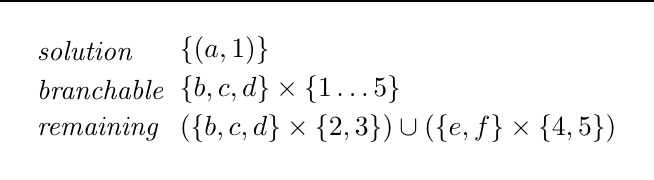
\begin{tikzpicture}[scale=0.33]
                    \node [anchor=west] (Ns) at (0, 3.5) { $\mathit{solution}$ };
                    \node [anchor=west] (Nb) at (0, 2) { $\mathit{branchable}$ };
                    \node [anchor=west] (Nr) at (0, 0.5) { $\mathit{remaining}$ };

                    \node [anchor=west] (Vs) at (5.5, 3.5) { $\{ (a, 1) \}$ };
                    \node [anchor=west] (Vb) at (5.5, 2) { $\{ b, c, d \} \times \{1 \ldots 5 \}$ };
                    \node [anchor=west] (Vr) at (5.5, 0.5) { $(\{ b, c, d \} \times \{ 2, 3 \}) \cup (\{ e, f\} \times \{ 4, 5 \})$ };
            \end{tikzpicture}
            \\[0.1cm]
            \stepcounter{stepcounter2}\roman{stepcounter2}) Initial problem &
            \stepcounter{stepcounter2}\roman{stepcounter2}) Search variables after guessing $a \mapsto 1$
            \\[0.4cm]
            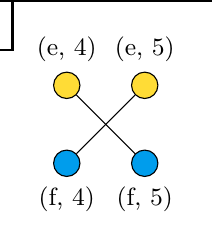
\begin{tikzpicture}[scale=0.33]
                    \node[draw, circle, fill=uofgsunshine, inner sep=0.5pt, font=\normalsize] (Me4) at (0, 3) {\phantom{0}};
                    \node[draw, circle, fill=uofgsunshine, inner sep=0.5pt, font=\normalsize] (Me5) at (3, 3) {\phantom{0}};
                    \node[draw, circle, fill=uofgcobalt, inner sep=0.5pt, font=\normalsize] (Mf4) at (0, 0) {\phantom{0}};
                    \node[draw, circle, fill=uofgcobalt, inner sep=0.5pt, font=\normalsize] (Mf5) at (3, 0) {\phantom{0}};

                    \node [above = 0 of Me4, font=\small] { \vphantom{0}(e, 4) };
                    \node [above = 0 of Me5, font=\small] { \vphantom{0}(e, 5) };
                    \node [below = 0 of Mf4, font=\small] { \vphantom{0}(f, 4) };
                    \node [below = 0 of Mf5, font=\small] { \vphantom{0}(f, 5) };

                    \draw (Me4) -- (Mf5);
                    \draw (Me5) -- (Mf4);
            \end{tikzpicture}
            &
            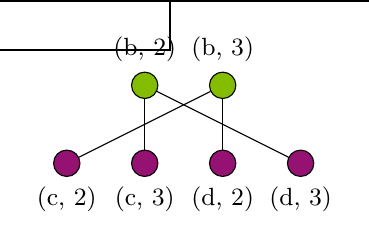
\begin{tikzpicture}[scale=0.33]
                    \node[draw, circle, fill=uofglawn, inner sep=0.5pt, font=\normalsize] (Mb2) at (3, 3) {\phantom{0}};
                    \node[draw, circle, fill=uofglawn, inner sep=0.5pt, font=\normalsize] (Mb3) at (6, 3) {\phantom{0}};
                    \node[draw, circle, fill=uofgthistle, inner sep=0.5pt, font=\normalsize] (Mc2) at (0, 0) {\phantom{0}};
                    \node[draw, circle, fill=uofgthistle, inner sep=0.5pt, font=\normalsize] (Mc3) at (3, 0) {\phantom{0}};
                    \node[draw, circle, fill=uofgthistle, inner sep=0.5pt, font=\normalsize] (Md2) at (6, 0) {\phantom{0}};
                    \node[draw, circle, fill=uofgthistle, inner sep=0.5pt, font=\normalsize] (Md3) at (9, 0) {\phantom{0}};

                    \node [above = 0 of Mb2, font=\small] { \vphantom{0}(b, 2) };
                    \node [above = 0 of Mb3, font=\small] { \vphantom{0}(b, 3) };
                    \node [below = 0 of Mc2, font=\small] { \vphantom{0}(c, 2) };
                    \node [below = 0 of Mc3, font=\small] { \vphantom{0}(c, 3) };
                    \node [below = 0 of Md2, font=\small] { \vphantom{0}(d, 2) };
                    \node [below = 0 of Md3, font=\small] { \vphantom{0}(d, 3) };

                    \draw (Mb2) -- (Mc3);
                    \draw (Mb2) -- (Md3);
                    \draw (Mb3) -- (Mc2);
                    \draw (Mb3) -- (Md2);
            \end{tikzpicture}
            \\[0.1cm]
            \stepcounter{stepcounter2}\roman{stepcounter2}) $\mathit{remaining} \setminus \mathit{branchable}$ &
            \stepcounter{stepcounter2}\roman{stepcounter2}) $\mathit{remaining} \cap \mathit{branchable}$
            \\
        };
    \end{tikzpicture}\\[0.3cm]\begin{tikzpicture}[scale=0.33]
        \matrix (m) [matrix of nodes] {
            \begin{tikzpicture}[scale=0.33]
                \node[draw, circle, fill=uofgsunshine, inner sep=0.5pt, font=\normalsize] (Me4) at (0, 0) {\phantom{0}};
                \node[draw, circle, fill=uofgsunshine, inner sep=0.5pt, font=\normalsize] (Me5) at (3, 0) {\phantom{0}};
                \node[draw, circle, fill=uofgcobalt, inner sep=0.5pt, font=\normalsize] (Mf4) at (6, 0) {\phantom{0}};
                \node[draw, circle, fill=uofgcobalt, inner sep=0.5pt, font=\normalsize] (Mf5) at (9, 0) {\phantom{0}};
                \node[draw, circle, fill=uofglawn, inner sep=0.5pt, font=\normalsize] (Mb2) at (12, 0) {\phantom{0}};
                \node[draw, circle, fill=uofglawn, inner sep=0.5pt, font=\normalsize] (Mb3) at (15, 0) {\phantom{0}};
                \node[draw, circle, fill=uofgthistle, inner sep=0.5pt, font=\normalsize] (Mc2) at (18, 0) {\phantom{0}};
                \node[draw, circle, fill=uofgthistle, inner sep=0.5pt, font=\normalsize] (Mc3) at (21, 0) {\phantom{0}};
                \node[draw, circle, fill=uofgthistle, inner sep=0.5pt, font=\normalsize] (Md2) at (24, 0) {\phantom{0}};
                \node[draw, circle, fill=uofgthistle, inner sep=0.5pt, font=\normalsize] (Md3) at (27, 0) {\phantom{0}};

                \node [above = 0 of Me4, font=\small, xshift=-0.5ex] { \vphantom{0}[[(e, 4), };
                \node [above = 0 of Me5, font=\small] { \vphantom{0}(e, 5)], };
                \node [above = 0 of Mf4, font=\small] { \vphantom{0}[(f, 4), };
                \node [above = 0 of Mf5, font=\small] { \vphantom{0}(f, 5)], };
                \node [above = 0 of Mb2, font=\small] { \vphantom{0}[(b, 2), };
                \node [above = 0 of Mb3, font=\small] { \vphantom{0}(b, 3)], };
                \node [above = 0 of Mc2, font=\small] { \vphantom{0}[(c, 2), };
                \node [above = 0 of Mc3, font=\small] { \vphantom{0}(c, 3), };
                \node [above = 0 of Md2, font=\small] { \vphantom{0}(d, 2), };
                \node [above = 0 of Md3, font=\small] { \vphantom{0}(d, 3)]]};
            \end{tikzpicture}
            \\[0.1cm]
            \stepcounter{stepcounter2}\roman{stepcounter2}) The resulting $\mathit{colourClasses}$ variable.
            \\
        };
    \end{tikzpicture}

    \caption{Solving a maximum common connected problem using an association graph. Suppose we
        have already mapped vertex $a$ to vertex $1$, giving the assignments on the right. Now we
        have two subgraphs to colour. We need two colours for $\mathit{remaining} \setminus
        \mathit{branchable}$, and we place these two colour classes first in the $\mathit{colourClasses}$
        variable. We can also colour $\mathit{remaining} \cap \mathit{branchable}$ using two
        colours, since we cannot simultaneously map $c$ to $2$ and $d$ to $3$, or vice-versa. Thus
        $\mathit{colourClasses}$ becomes a list of four colour classes, the first three containing
        two vertices each, and the last containing four vertices. This tells us that if we hope to
        extend the current common subgraph by another four vertices, we
        must pick one assignment from each of the four colour classes (which is not actually possible, so we
    see the bound here gives an overestimate). The algorithm thus guesses $d \mapsto 3$ as its next
assignment, and if that fails, $d \mapsto 2$, and so on; once $b \mapsto 3$ is reached, the bound
decreases by one, and if $f \mapsto 5$ were reached we would stop due to a lack of remaining
branchable vertices. }\label{figure:assocrestricted}
\end{figure}

It is not possible to determine connectedness from a raw association graph. However, we can take a
maximum clique algorithm and mimic the branching strategy if we have access to the underlying graphs
and can determine the ``meaning'' of the association graph vertices.

Most modern maximum clique algorithms for dense graphs use some variation of greedy graph colouring
as a bound---the underlying observation is that each vertex in a clique must be given a different
colour in a colouring, so if we can colour a subset of vertices using $k$ colours then a maximum
clique in this subset has at most $k$ vertices. However, the colouring is also used as a branching
heuristic: vertices are selected in reverse from their colour classes in turn, starting with the
last colour class created. Because of this coupling of branching and the bound (which is important
in practice because it mimics a ``smallest domain first'' branching heuristic if colour classes are
viewed as variables \cite{DBLP:conf/cp/McCreeshP14}), if we were to select only a subset of vertices for
branching at each stage inside a clique algorithm, we would lose completeness. Thus we must adapt
the bound to take into account restricted branching.

In \cref{algorithm:mccis} we present a clique-inspired algorithm which finds a maximum common
connected induced subgraph isomorphism via an
association graph. If the additional
branching restrictions are removed, the core of the algorithm is what Prosser
\cite{DBLP:journals/algorithms/Prosser12} calls the ``MCSa1'' variant of a series of algorithms due
to Tomita \textit{et al.}\
\cite{DBLP:conf/dmtcs/TomitaS03,DBLP:journals/jgo/TomitaK07,DBLP:conf/walcom/TomitaSHTW10}, using a
bitset encoding approach due to San Segundo \textit{et al.}\
\cite{DBLP:journals/cor/SegundoRJ11,DBLP:journals/ol/SegundoMRH13} (and we refer the reader to these
papers for implementation details on how to use bitsets and other data structures to implement the
colouring stage with very low constant factors).

We begin by building the association graph (\lineref{buildassoc}). The main part of the algorithm
then works by building up candidate cliques in the $\mathit{solution}$ variable, by recursive calls
to the $\mathit{search}$ procedure---starting from the empty set (\lineref{firstsearch}), each
recursive subcall adds one vertex to $\mathit{solution}$ (\lineref{addv}) in such a way that
$\mathit{solution}$ is always a clique which corresponds to a connected common subgraph. The
$\mathit{remaining}$ set contains the set of vertices which are adjacent to every vertex in
$\mathit{solution}$, and which have not yet been accepted or rejected (and so initially it contains
every vertex). The main loops in the $\FuncSty{search}$ procedure
(\twolinesref{outerloop}{innerloop}) have the effect of iterating over each vertex in this set in a
particular order---each vertex $v$ is selected in turn, and then a recursive call is made to
consider the effects of including $v$ in $\mathit{solution}$ (\lineref{recursesearch}), followed by
the next iteration where $v$ is instead rejected. When $v$ is accepted, we add it to the new
$\mathit{solution'}$ (\lineref{addvtosolution}), and create a new $\mathit{remaining'}$ containing
only the vertices in $\mathit{remaining}$ which are adjacent to $v$ (\lineref{filterremaining}).

The $\mathit{branchable}$ set contains the set of association graph vertices which correspond to
vertices adjacent to an already-accepted vertex in the first input graph---in constraint programming terms, it is the
set of assignments which could be made next which preserve connectedness. (Using only one of the two
input graphs is sufficient for correctness, and has the advantage that the $\FuncSty{connected}$
function may be implemented as a simple lookup into a precomputed array which maps each vertex in
the first input graph to a bitset.) At the top of search, this set is empty, and is not used (our
first vertex selection is special, and does not care about connectedness). At subsequent depths, we
may only accept vertices which are in this set, and if no such vertices remain then we return
immediately (\lineref{acceptbranchable}). When recursing, we extend $\mathit{branchable}$ with the
new vertices permitted by our acceptance of the branching $v$ (\lineref{addtobranchable}). Note that
we are assuming that inside the main loops, we encounter every vertex in $\mathit{remaining} \cap
\mathit{connected}$ before any vertex in $\mathit{remaining} \setminus \mathit{connected}$.

As we proceed, we keep track of the best solution we have found so far---this is stored in the
$\mathit{incumbent}$ variable (\twolinesref{incumbent}{newincumbent}). We use the incumbent,
together with a colour bound, to prune portions of the search space which cannot contain a better
solution. The colour bound operates as follows: at each entry to the $\FuncSty{search}$ procedure,
we produce a greedy colouring of the vertices in $\mathit{remaining}$ (\lineref{makecolours}). This
greedy colouring gives us a list of colour classes, each of which is a list of pairwise non-adjacent
vertices. The two loops (\twolinesref{outerloop}{innerloop}) then iterate over each colour class,
from last to first, and then over each vertex in that colour class, again from last to first.
(Rather than actually using a list of lists and removing items, this process should be implemented
using a pair of immutable flat arrays. This technique is described elsewhere
\cite{DBLP:conf/cp/McCreeshP14}, so we do not discuss it here.) Finally, if at any point the number
of remaining colour classes plus the number of vertices currently present in $\mathit{solution}$ is
not strictly greater than the size of the incumbent, then we may backtrack immediately
(\lineref{bound}).

Finally, we describe the colouring process. In conventional clique algorithms, a simple greedy
sequential colouring is used (possibly with the help of previous colourings to reduce the
computational cost \cite{DBLP:conf/lion/NikolaevBS15}, and possibly with shortcuts taken for certain
vertices \cite{DBLP:journals/cor/SegundoT14}, and possibly followed by a repair step to
improve the colouring \cite{DBLP:conf/walcom/TomitaSHTW10}, or stronger bounding rules based upon
MaxSAT inference \cite{DBLP:conf/ictai/LiFX13,DBLP:conf/lion/LiJX15,DBLP:journals/cor/SegundoNB15}).
Such colourings will not give us the required property that vertices in $\mathit{remaining} \cap
\mathit{connected}$ come last (so they are selected first by the reverse branching order). Thus we
produce two greedy sequential colourings, first considering the non-branching vertices in
$\mathit{remaining} \setminus \mathit{connected}$, followed by the branching vertices, and
concatenate them (\lineref{makecolours}). This produces a valid colouring, since we do not merge any
colour classes between the two stages, although it may use more colours than a single colouring
would\footnote{What if we did not guarantee that vertices in $\mathit{remaining} \cap
    \mathit{connected}$ came last, and just used a conventional colouring with the branching rule?
    Suppose we had four vertices in $\mathit{remaining}$, and produced a colouring $[[v_1, v_2],
    [v_3], [v_4]]$, and suppose that extending $\mathit{solution}$ with $\{ v_1, v_3, v_4 \}$ gives
an optimal solution. If $v_4$ was not $\mathit{connected}$ yet, we would not branch on that subtree,
and the bound could eliminate branching on $v_3$ and $v_1$, so we would miss the solution. Thus we
cannot simply add the branching rule without also adapting the combined bound / ordering heuristic.}.

Our $\FuncSty{colour}$ procedure is the same as the bit-parallel algorithm introduced by San Segundo
\textit{et al.}\ \cite{DBLP:journals/cor/SegundoRJ11}. While we have remaining vertices to colour
(\lineref{whileuncoloured}), we start a new colour class (\lineref{newcolourclass}), and then
repeatedly pick a legal vertex to add to that colour class (\lineref{addtocolourclass}).  The
selection of the next vertex to colour (\lineref{selectvtocolour}) may be performed efficiently in
hardware if the association graph is permuted to be in degree order at the top of search. Other
initial vertex orderings have been considered on general clique problems
\cite{DBLP:journals/algorithms/Prosser12,DBLP:conf/lion/SegundoLB14}; it is possible that special
properties of the association graph could be exploited in this step.

\subsection{Experimental Evaluation}

\paragraph{Connected, Undirected, 33\% Labelled}

\paragraph{Connected, Undirected, Unlabelled}

?? My gut feeling is that if we have edge labels, the clique model wins, and if we don't, it's
likely to lose. So maybe I should run some experiments with vertex labels but not edge labels to
test this.

\paragraph{By family} ?? Break this down more by family, size, etc.

\paragraph{Does connected make instances easier or harder?} We could plot connected vs not connected
difficulties, and result sizes?

\begin{figure}[p]
    \centering
    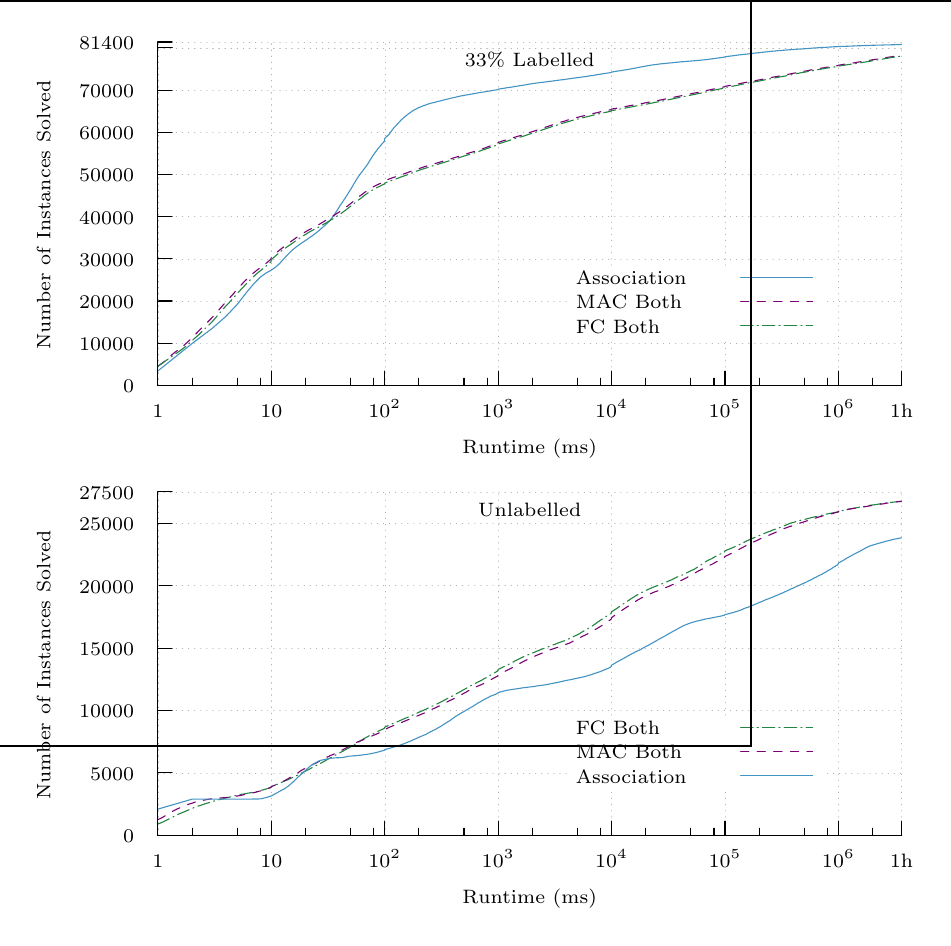
\begin{tikzpicture}[gnuplot]
%% generated with GNUPLOT 5.0p0 (Lua 5.2; terminal rev. 99, script rev. 100)
%% Tue 19 Apr 2016 16:47:16 AEST
\tikzset{every node/.append style={font={\scriptsize}}}
% \path (0.000,0.000) rectangle (11.684,11.430);
\gpcolor{color=gp lt color axes}
\gpsetlinetype{gp lt axes}
\gpsetdashtype{gp dt axes}
\gpsetlinewidth{0.50}
\draw[gp path] (1.688,10.986)--(11.131,10.986);
\gpcolor{color=gp lt color border}
\gpsetlinetype{gp lt border}
\gpsetdashtype{gp dt solid}
\gpsetlinewidth{1.00}
\draw[gp path] (1.688,10.986)--(1.868,10.986);
\gpcolor{color=gp lt color axes}
\gpsetlinetype{gp lt axes}
\gpsetdashtype{gp dt axes}
\gpsetlinewidth{0.50}
\draw[gp path] (1.688,11.061)--(11.131,11.061);
\gpcolor{color=gp lt color border}
\gpsetlinetype{gp lt border}
\gpsetdashtype{gp dt solid}
\gpsetlinewidth{1.00}
\draw[gp path] (1.688,11.061)--(1.868,11.061);
\node[gp node right] at (1.504,11.061) {81400};
\gpcolor{color=gp lt color axes}
\gpsetlinetype{gp lt axes}
\gpsetdashtype{gp dt axes}
\gpsetlinewidth{0.50}
\draw[gp path] (1.688,6.700)--(11.131,6.700);
\gpcolor{color=gp lt color border}
\gpsetlinetype{gp lt border}
\gpsetdashtype{gp dt solid}
\gpsetlinewidth{1.00}
\draw[gp path] (1.688,6.700)--(1.868,6.700);
\node[gp node right] at (1.504,6.700) {$0$};
\gpcolor{color=gp lt color axes}
\gpsetlinetype{gp lt axes}
\gpsetdashtype{gp dt axes}
\gpsetlinewidth{0.50}
\draw[gp path] (1.688,7.236)--(11.131,7.236);
\gpcolor{color=gp lt color border}
\gpsetlinetype{gp lt border}
\gpsetdashtype{gp dt solid}
\gpsetlinewidth{1.00}
\draw[gp path] (1.688,7.236)--(1.868,7.236);
\node[gp node right] at (1.504,7.236) {$10000$};
\gpcolor{color=gp lt color axes}
\gpsetlinetype{gp lt axes}
\gpsetdashtype{gp dt axes}
\gpsetlinewidth{0.50}
\draw[gp path] (1.688,7.771)--(6.879,7.771);
\draw[gp path] (10.187,7.771)--(11.131,7.771);
\gpcolor{color=gp lt color border}
\gpsetlinetype{gp lt border}
\gpsetdashtype{gp dt solid}
\gpsetlinewidth{1.00}
\draw[gp path] (1.688,7.771)--(1.868,7.771);
\node[gp node right] at (1.504,7.771) {$20000$};
\gpcolor{color=gp lt color axes}
\gpsetlinetype{gp lt axes}
\gpsetdashtype{gp dt axes}
\gpsetlinewidth{0.50}
\draw[gp path] (1.688,8.307)--(11.131,8.307);
\gpcolor{color=gp lt color border}
\gpsetlinetype{gp lt border}
\gpsetdashtype{gp dt solid}
\gpsetlinewidth{1.00}
\draw[gp path] (1.688,8.307)--(1.868,8.307);
\node[gp node right] at (1.504,8.307) {$30000$};
\gpcolor{color=gp lt color axes}
\gpsetlinetype{gp lt axes}
\gpsetdashtype{gp dt axes}
\gpsetlinewidth{0.50}
\draw[gp path] (1.688,8.843)--(11.131,8.843);
\gpcolor{color=gp lt color border}
\gpsetlinetype{gp lt border}
\gpsetdashtype{gp dt solid}
\gpsetlinewidth{1.00}
\draw[gp path] (1.688,8.843)--(1.868,8.843);
\node[gp node right] at (1.504,8.843) {$40000$};
\gpcolor{color=gp lt color axes}
\gpsetlinetype{gp lt axes}
\gpsetdashtype{gp dt axes}
\gpsetlinewidth{0.50}
\draw[gp path] (1.688,9.379)--(11.131,9.379);
\gpcolor{color=gp lt color border}
\gpsetlinetype{gp lt border}
\gpsetdashtype{gp dt solid}
\gpsetlinewidth{1.00}
\draw[gp path] (1.688,9.379)--(1.868,9.379);
\node[gp node right] at (1.504,9.379) {$50000$};
\gpcolor{color=gp lt color axes}
\gpsetlinetype{gp lt axes}
\gpsetdashtype{gp dt axes}
\gpsetlinewidth{0.50}
\draw[gp path] (1.688,9.914)--(11.131,9.914);
\gpcolor{color=gp lt color border}
\gpsetlinetype{gp lt border}
\gpsetdashtype{gp dt solid}
\gpsetlinewidth{1.00}
\draw[gp path] (1.688,9.914)--(1.868,9.914);
\node[gp node right] at (1.504,9.914) {$60000$};
\gpcolor{color=gp lt color axes}
\gpsetlinetype{gp lt axes}
\gpsetdashtype{gp dt axes}
\gpsetlinewidth{0.50}
\draw[gp path] (1.688,10.450)--(11.131,10.450);
\gpcolor{color=gp lt color border}
\gpsetlinetype{gp lt border}
\gpsetdashtype{gp dt solid}
\gpsetlinewidth{1.00}
\draw[gp path] (1.688,10.450)--(1.868,10.450);
\node[gp node right] at (1.504,10.450) {$70000$};
\gpcolor{color=gp lt color axes}
\gpsetlinetype{gp lt axes}
\gpsetdashtype{gp dt axes}
\gpsetlinewidth{0.50}
\draw[gp path] (1.688,10.986)--(11.131,10.986);
\gpcolor{color=gp lt color border}
\gpsetlinetype{gp lt border}
\gpsetdashtype{gp dt solid}
\gpsetlinewidth{1.00}
\draw[gp path] (1.688,10.986)--(1.868,10.986);
\gpcolor{color=gp lt color axes}
\gpsetlinetype{gp lt axes}
\gpsetdashtype{gp dt axes}
\gpsetlinewidth{0.50}
\draw[gp path] (1.688,6.700)--(1.688,11.061);
\gpcolor{color=gp lt color border}
\gpsetlinetype{gp lt border}
\gpsetdashtype{gp dt solid}
\gpsetlinewidth{1.00}
\draw[gp path] (1.688,6.700)--(1.688,6.880);
\node[gp node center] at (1.688,6.392) {1};
\gpcolor{color=gp lt color axes}
\gpsetlinetype{gp lt axes}
\gpsetdashtype{gp dt axes}
\gpsetlinewidth{0.50}
\draw[gp path] (3.128,6.700)--(3.128,11.061);
\gpcolor{color=gp lt color border}
\gpsetlinetype{gp lt border}
\gpsetdashtype{gp dt solid}
\gpsetlinewidth{1.00}
\draw[gp path] (3.128,6.700)--(3.128,6.880);
\node[gp node center] at (3.128,6.392) {10};
\gpcolor{color=gp lt color axes}
\gpsetlinetype{gp lt axes}
\gpsetdashtype{gp dt axes}
\gpsetlinewidth{0.50}
\draw[gp path] (11.131,6.700)--(11.131,11.061);
\gpcolor{color=gp lt color border}
\gpsetlinetype{gp lt border}
\gpsetdashtype{gp dt solid}
\gpsetlinewidth{1.00}
\draw[gp path] (11.131,6.700)--(11.131,6.880);
\node[gp node center] at (11.131,6.392) {1h};
\gpcolor{color=gp lt color axes}
\gpsetlinetype{gp lt axes}
\gpsetdashtype{gp dt axes}
\gpsetlinewidth{0.50}
\draw[gp path] (1.688,6.700)--(1.688,11.061);
\gpcolor{color=gp lt color border}
\gpsetlinetype{gp lt border}
\gpsetdashtype{gp dt solid}
\gpsetlinewidth{1.00}
\draw[gp path] (1.688,6.700)--(1.688,6.880);
\draw[gp path] (2.122,6.700)--(2.122,6.790);
\draw[gp path] (2.695,6.700)--(2.695,6.790);
\draw[gp path] (2.989,6.700)--(2.989,6.790);
\gpcolor{color=gp lt color axes}
\gpsetlinetype{gp lt axes}
\gpsetdashtype{gp dt axes}
\gpsetlinewidth{0.50}
\draw[gp path] (3.128,6.700)--(3.128,11.061);
\gpcolor{color=gp lt color border}
\gpsetlinetype{gp lt border}
\gpsetdashtype{gp dt solid}
\gpsetlinewidth{1.00}
\draw[gp path] (3.128,6.700)--(3.128,6.880);
\draw[gp path] (3.562,6.700)--(3.562,6.790);
\draw[gp path] (4.135,6.700)--(4.135,6.790);
\draw[gp path] (4.429,6.700)--(4.429,6.790);
\gpcolor{color=gp lt color axes}
\gpsetlinetype{gp lt axes}
\gpsetdashtype{gp dt axes}
\gpsetlinewidth{0.50}
\draw[gp path] (4.569,6.700)--(4.569,11.061);
\gpcolor{color=gp lt color border}
\gpsetlinetype{gp lt border}
\gpsetdashtype{gp dt solid}
\gpsetlinewidth{1.00}
\draw[gp path] (4.569,6.700)--(4.569,6.880);
\node[gp node center] at (4.569,6.392) {$10^{2}$};
\draw[gp path] (5.002,6.700)--(5.002,6.790);
\draw[gp path] (5.575,6.700)--(5.575,6.790);
\draw[gp path] (5.869,6.700)--(5.869,6.790);
\gpcolor{color=gp lt color axes}
\gpsetlinetype{gp lt axes}
\gpsetdashtype{gp dt axes}
\gpsetlinewidth{0.50}
\draw[gp path] (6.009,6.700)--(6.009,11.061);
\gpcolor{color=gp lt color border}
\gpsetlinetype{gp lt border}
\gpsetdashtype{gp dt solid}
\gpsetlinewidth{1.00}
\draw[gp path] (6.009,6.700)--(6.009,6.880);
\node[gp node center] at (6.009,6.392) {$10^{3}$};
\draw[gp path] (6.442,6.700)--(6.442,6.790);
\draw[gp path] (7.016,6.700)--(7.016,6.790);
\draw[gp path] (7.310,6.700)--(7.310,6.790);
\gpcolor{color=gp lt color axes}
\gpsetlinetype{gp lt axes}
\gpsetdashtype{gp dt axes}
\gpsetlinewidth{0.50}
\draw[gp path] (7.449,6.700)--(7.449,7.302);
\draw[gp path] (7.449,8.226)--(7.449,11.061);
\gpcolor{color=gp lt color border}
\gpsetlinetype{gp lt border}
\gpsetdashtype{gp dt solid}
\gpsetlinewidth{1.00}
\draw[gp path] (7.449,6.700)--(7.449,6.880);
\node[gp node center] at (7.449,6.392) {$10^{4}$};
\draw[gp path] (7.883,6.700)--(7.883,6.790);
\draw[gp path] (8.456,6.700)--(8.456,6.790);
\draw[gp path] (8.750,6.700)--(8.750,6.790);
\gpcolor{color=gp lt color axes}
\gpsetlinetype{gp lt axes}
\gpsetdashtype{gp dt axes}
\gpsetlinewidth{0.50}
\draw[gp path] (8.889,6.700)--(8.889,7.302);
\draw[gp path] (8.889,8.226)--(8.889,11.061);
\gpcolor{color=gp lt color border}
\gpsetlinetype{gp lt border}
\gpsetdashtype{gp dt solid}
\gpsetlinewidth{1.00}
\draw[gp path] (8.889,6.700)--(8.889,6.880);
\node[gp node center] at (8.889,6.392) {$10^{5}$};
\draw[gp path] (9.323,6.700)--(9.323,6.790);
\draw[gp path] (9.896,6.700)--(9.896,6.790);
\draw[gp path] (10.190,6.700)--(10.190,6.790);
\gpcolor{color=gp lt color axes}
\gpsetlinetype{gp lt axes}
\gpsetdashtype{gp dt axes}
\gpsetlinewidth{0.50}
\draw[gp path] (10.330,6.700)--(10.330,11.061);
\gpcolor{color=gp lt color border}
\gpsetlinetype{gp lt border}
\gpsetdashtype{gp dt solid}
\gpsetlinewidth{1.00}
\draw[gp path] (10.330,6.700)--(10.330,6.880);
\node[gp node center] at (10.330,6.392) {$10^{6}$};
\draw[gp path] (10.763,6.700)--(10.763,6.790);
\draw[gp path] (1.688,11.061)--(1.688,6.700)--(11.131,6.700);
\node[gp node center,rotate=-270] at (0.246,8.880) {Number of Instances Solved};
\node[gp node center] at (6.409,5.930) {Runtime (ms)};
\node[gp node left] at (6.879,8.072) {Association};
\gpcolor{rgb color={0.263,0.576,0.765}}
\draw[gp path] (9.087,8.072)--(10.003,8.072);
\draw[gp path] (1.688,6.884)--(2.122,7.232)--(2.375,7.422)--(2.555,7.580)--(2.695,7.728)%
  --(2.809,7.876)--(2.905,7.990)--(2.989,8.075)--(3.062,8.127)--(3.128,8.164)--(3.188,8.205)%
  --(3.242,8.257)--(3.292,8.313)--(3.339,8.364)--(3.382,8.407)--(3.422,8.441)--(3.460,8.470)%
  --(3.496,8.496)--(3.530,8.519)--(3.562,8.540)--(3.592,8.560)--(3.621,8.582)--(3.649,8.599)%
  --(3.676,8.621)--(3.701,8.640)--(3.726,8.660)--(3.750,8.681)--(3.772,8.701)--(3.794,8.719)%
  --(3.815,8.738)--(3.836,8.756)--(3.856,8.776)--(3.875,8.799)--(3.894,8.823)--(3.912,8.846)%
  --(3.930,8.871)--(3.947,8.898)--(3.963,8.922)--(3.980,8.948)--(3.995,8.974)--(4.011,8.998)%
  --(4.026,9.018)--(4.041,9.041)--(4.055,9.062)--(4.069,9.084)--(4.083,9.104)--(4.096,9.126)%
  --(4.109,9.147)--(4.122,9.169)--(4.135,9.188)--(4.147,9.209)--(4.160,9.229)--(4.171,9.250)%
  --(4.183,9.270)--(4.195,9.290)--(4.206,9.309)--(4.217,9.325)--(4.228,9.343)--(4.239,9.360)%
  --(4.249,9.375)--(4.259,9.387)--(4.270,9.401)--(4.280,9.413)--(4.289,9.424)--(4.299,9.438)%
  --(4.309,9.452)--(4.318,9.464)--(4.327,9.476)--(4.336,9.488)--(4.345,9.501)--(4.354,9.514)%
  --(4.363,9.529)--(4.372,9.545)--(4.380,9.558)--(4.389,9.571)--(4.397,9.584)--(4.405,9.597)%
  --(4.413,9.610)--(4.421,9.622)--(4.429,9.632)--(4.437,9.644)--(4.444,9.656)--(4.452,9.665)%
  --(4.460,9.675)--(4.467,9.684)--(4.474,9.695)--(4.481,9.704)--(4.489,9.713)--(4.496,9.722)%
  --(4.503,9.731)--(4.510,9.738)--(4.516,9.746)--(4.523,9.754)--(4.530,9.763)--(4.537,9.769)%
  --(4.543,9.777)--(4.550,9.784)--(4.556,9.791)--(4.562,9.798)--(4.569,9.837)--(4.628,9.894)%
  --(4.683,9.970)--(4.733,10.022)--(4.779,10.073)--(4.822,10.110)--(4.863,10.144)--(4.901,10.170)%
  --(4.936,10.195)--(4.970,10.212)--(5.002,10.229)--(5.033,10.240)--(5.062,10.253)--(5.090,10.261)%
  --(5.116,10.272)--(5.142,10.279)--(5.166,10.286)--(5.190,10.291)--(5.213,10.298)--(5.235,10.303)%
  --(5.256,10.309)--(5.276,10.313)--(5.296,10.319)--(5.315,10.324)--(5.334,10.329)--(5.352,10.332)%
  --(5.370,10.337)--(5.387,10.341)--(5.404,10.345)--(5.420,10.350)--(5.436,10.353)--(5.451,10.356)%
  --(5.466,10.359)--(5.481,10.363)--(5.495,10.367)--(5.509,10.369)--(5.523,10.373)--(5.537,10.376)%
  --(5.550,10.378)--(5.563,10.380)--(5.575,10.383)--(5.588,10.385)--(5.600,10.387)--(5.612,10.389)%
  --(5.623,10.391)--(5.635,10.393)--(5.646,10.395)--(5.657,10.397)--(5.668,10.399)--(5.679,10.400)%
  --(5.689,10.403)--(5.700,10.405)--(5.710,10.407)--(5.720,10.408)--(5.730,10.410)--(5.739,10.412)%
  --(5.749,10.414)--(5.758,10.415)--(5.768,10.417)--(5.777,10.419)--(5.786,10.420)--(5.795,10.421)%
  --(5.803,10.422)--(5.812,10.424)--(5.821,10.425)--(5.829,10.426)--(5.837,10.428)--(5.845,10.429)%
  --(5.853,10.431)--(5.861,10.432)--(5.869,10.434)--(5.877,10.435)--(5.885,10.436)--(5.892,10.437)%
  --(5.900,10.438)--(5.907,10.439)--(5.915,10.441)--(5.922,10.442)--(5.929,10.443)--(5.936,10.445)%
  --(5.943,10.446)--(5.950,10.447)--(5.957,10.449)--(5.963,10.449)--(5.970,10.450)--(5.977,10.451)%
  --(5.983,10.452)--(5.990,10.453)--(5.996,10.455)--(6.003,10.456)--(6.009,10.462)--(6.068,10.471)%
  --(6.123,10.480)--(6.173,10.487)--(6.219,10.495)--(6.263,10.502)--(6.303,10.509)--(6.341,10.514)%
  --(6.377,10.521)--(6.410,10.527)--(6.442,10.532)--(6.473,10.536)--(6.502,10.540)--(6.530,10.544)%
  --(6.556,10.547)--(6.582,10.550)--(6.607,10.553)--(6.630,10.557)--(6.653,10.560)--(6.675,10.562)%
  --(6.696,10.564)--(6.717,10.568)--(6.736,10.571)--(6.756,10.573)--(6.774,10.575)--(6.792,10.578)%
  --(6.810,10.580)--(6.827,10.582)--(6.844,10.584)--(6.860,10.586)--(6.876,10.589)--(6.891,10.591)%
  --(6.907,10.593)--(6.921,10.595)--(6.936,10.597)--(6.950,10.599)--(6.963,10.601)--(6.977,10.603)%
  --(6.990,10.604)--(7.003,10.606)--(7.016,10.608)--(7.028,10.610)--(7.040,10.611)--(7.052,10.613)%
  --(7.064,10.615)--(7.075,10.616)--(7.086,10.618)--(7.098,10.619)--(7.108,10.621)--(7.119,10.622)%
  --(7.130,10.624)--(7.140,10.625)--(7.150,10.627)--(7.160,10.629)--(7.170,10.630)--(7.180,10.631)%
  --(7.189,10.633)--(7.199,10.634)--(7.208,10.635)--(7.217,10.637)--(7.226,10.638)--(7.235,10.640)%
  --(7.244,10.642)--(7.252,10.644)--(7.261,10.645)--(7.269,10.646)--(7.278,10.648)--(7.286,10.649)%
  --(7.294,10.650)--(7.302,10.651)--(7.310,10.653)--(7.317,10.654)--(7.325,10.655)--(7.333,10.656)%
  --(7.340,10.658)--(7.348,10.659)--(7.355,10.660)--(7.362,10.661)--(7.369,10.662)--(7.376,10.662)%
  --(7.383,10.664)--(7.390,10.665)--(7.397,10.666)--(7.404,10.667)--(7.410,10.668)--(7.417,10.669)%
  --(7.424,10.670)--(7.430,10.671)--(7.437,10.672)--(7.443,10.673)--(7.449,10.679)--(7.509,10.689)%
  --(7.563,10.697)--(7.613,10.705)--(7.660,10.713)--(7.703,10.721)--(7.743,10.728)--(7.781,10.736)%
  --(7.817,10.743)--(7.851,10.749)--(7.883,10.755)--(7.913,10.761)--(7.942,10.765)--(7.970,10.770)%
  --(7.997,10.773)--(8.022,10.776)--(8.047,10.780)--(8.070,10.783)--(8.093,10.785)--(8.115,10.787)%
  --(8.136,10.789)--(8.157,10.791)--(8.177,10.794)--(8.196,10.795)--(8.215,10.797)--(8.233,10.799)%
  --(8.250,10.801)--(8.268,10.803)--(8.284,10.804)--(8.300,10.806)--(8.316,10.807)--(8.332,10.809)%
  --(8.347,10.810)--(8.362,10.811)--(8.376,10.812)--(8.390,10.813)--(8.404,10.815)--(8.417,10.816)%
  --(8.430,10.817)--(8.443,10.818)--(8.456,10.819)--(8.468,10.820)--(8.480,10.821)--(8.492,10.822)%
  --(8.504,10.823)--(8.516,10.824)--(8.527,10.825)--(8.538,10.826)--(8.549,10.827)--(8.559,10.828)%
  --(8.570,10.829)--(8.580,10.830)--(8.590,10.831)--(8.600,10.832)--(8.610,10.833)--(8.620,10.834)%
  --(8.630,10.835)--(8.639,10.836)--(8.648,10.837)--(8.657,10.838)--(8.666,10.839)--(8.675,10.840)%
  --(8.684,10.841)--(8.693,10.843)--(8.701,10.844)--(8.710,10.845)--(8.718,10.846)--(8.726,10.848)%
  --(8.734,10.848)--(8.742,10.849)--(8.750,10.850)--(8.758,10.851)--(8.765,10.853)--(8.773,10.854)%
  --(8.780,10.855)--(8.788,10.856)--(8.795,10.856)--(8.802,10.857)--(8.810,10.858)--(8.817,10.860)%
  --(8.824,10.861)--(8.830,10.862)--(8.837,10.863)--(8.844,10.863)--(8.851,10.864)--(8.857,10.865)%
  --(8.864,10.866)--(8.870,10.867)--(8.877,10.868)--(8.883,10.869)--(8.889,10.873)--(8.949,10.881)%
  --(9.004,10.888)--(9.054,10.895)--(9.100,10.900)--(9.143,10.905)--(9.183,10.909)--(9.221,10.914)%
  --(9.257,10.919)--(9.291,10.922)--(9.323,10.925)--(9.354,10.929)--(9.383,10.932)--(9.410,10.935)%
  --(9.437,10.938)--(9.463,10.941)--(9.487,10.943)--(9.511,10.945)--(9.534,10.947)--(9.555,10.950)%
  --(9.577,10.951)--(9.597,10.953)--(9.617,10.955)--(9.636,10.956)--(9.655,10.958)--(9.673,10.959)%
  --(9.691,10.961)--(9.708,10.962)--(9.725,10.963)--(9.741,10.964)--(9.757,10.966)--(9.772,10.967)%
  --(9.787,10.968)--(9.802,10.969)--(9.816,10.970)--(9.830,10.971)--(9.844,10.972)--(9.857,10.972)%
  --(9.871,10.973)--(9.884,10.974)--(9.896,10.975)--(9.909,10.976)--(9.921,10.976)--(9.933,10.977)%
  --(9.944,10.978)--(9.956,10.979)--(9.967,10.980)--(9.978,10.981)--(9.989,10.982)--(10.000,10.983)%
  --(10.010,10.984)--(10.021,10.984)--(10.031,10.985)--(10.041,10.986)--(10.051,10.986)--(10.060,10.987)%
  --(10.070,10.988)--(10.079,10.988)--(10.089,10.989)--(10.098,10.990)--(10.107,10.990)--(10.116,10.991)%
  --(10.124,10.991)--(10.133,10.991)--(10.141,10.992)--(10.150,10.992)--(10.158,10.993)--(10.166,10.993)%
  --(10.174,10.993)--(10.182,10.994)--(10.190,10.995)--(10.198,10.995)--(10.206,10.996)--(10.213,10.996)%
  --(10.221,10.997)--(10.228,10.997)--(10.235,10.997)--(10.243,10.998)--(10.250,10.998)--(10.257,10.998)%
  --(10.264,10.999)--(10.271,11.000)--(10.278,11.000)--(10.284,11.000)--(10.291,11.001)--(10.298,11.001)%
  --(10.304,11.001)--(10.311,11.002)--(10.317,11.002)--(10.323,11.002)--(10.330,11.003)--(10.389,11.005)%
  --(10.444,11.007)--(10.494,11.009)--(10.540,11.011)--(10.583,11.013)--(10.624,11.014)--(10.662,11.016)%
  --(10.697,11.016)--(10.731,11.018)--(10.763,11.019)--(10.794,11.020)--(10.823,11.021)--(10.851,11.022)%
  --(10.877,11.022)--(10.903,11.023)--(10.927,11.024)--(10.951,11.024)--(10.974,11.025)--(10.996,11.025)%
  --(11.017,11.026)--(11.037,11.026)--(11.057,11.027)--(11.077,11.027)--(11.095,11.028)--(11.113,11.028)%
  --(11.131,11.028);
\gpcolor{color=gp lt color border}
\node[gp node left] at (6.879,7.764) {MAC Both};
\gpcolor{rgb color={0.478,0.004,0.467}}
\gpsetdashtype{gp dt 2}
\draw[gp path] (9.087,7.764)--(10.003,7.764);
\draw[gp path] (1.688,6.944)--(1.748,6.987)--(1.802,7.034)--(1.852,7.077)--(1.898,7.116)%
  --(1.942,7.148)--(1.982,7.180)--(2.020,7.210)--(2.056,7.242)--(2.089,7.273)--(2.122,7.304)%
  --(2.152,7.337)--(2.181,7.365)--(2.209,7.395)--(2.236,7.423)--(2.261,7.447)--(2.286,7.474)%
  --(2.309,7.494)--(2.332,7.516)--(2.354,7.538)--(2.375,7.560)--(2.396,7.583)--(2.416,7.606)%
  --(2.435,7.627)--(2.453,7.649)--(2.472,7.669)--(2.489,7.689)--(2.506,7.709)--(2.523,7.728)%
  --(2.539,7.744)--(2.555,7.761)--(2.571,7.776)--(2.586,7.794)--(2.600,7.812)--(2.615,7.829)%
  --(2.629,7.844)--(2.643,7.859)--(2.656,7.874)--(2.669,7.891)--(2.682,7.905)--(2.695,7.919)%
  --(2.707,7.933)--(2.719,7.946)--(2.731,7.958)--(2.743,7.972)--(2.754,7.985)--(2.766,7.998)%
  --(2.777,8.010)--(2.788,8.021)--(2.798,8.032)--(2.809,8.041)--(2.819,8.050)--(2.829,8.060)%
  --(2.839,8.070)--(2.849,8.078)--(2.859,8.089)--(2.868,8.098)--(2.878,8.107)--(2.887,8.115)%
  --(2.896,8.123)--(2.905,8.130)--(2.914,8.138)--(2.923,8.144)--(2.931,8.152)--(2.940,8.158)%
  --(2.948,8.165)--(2.957,8.171)--(2.965,8.178)--(2.973,8.184)--(2.981,8.189)--(2.989,8.196)%
  --(2.996,8.202)--(3.004,8.207)--(3.012,8.213)--(3.019,8.219)--(3.027,8.224)--(3.034,8.229)%
  --(3.041,8.235)--(3.048,8.240)--(3.055,8.246)--(3.062,8.251)--(3.069,8.256)--(3.076,8.262)%
  --(3.083,8.268)--(3.090,8.274)--(3.096,8.278)--(3.103,8.285)--(3.109,8.291)--(3.116,8.296)%
  --(3.122,8.301)--(3.128,8.330)--(3.188,8.381)--(3.242,8.425)--(3.292,8.464)--(3.339,8.499)%
  --(3.382,8.531)--(3.422,8.559)--(3.460,8.586)--(3.496,8.610)--(3.530,8.631)--(3.562,8.650)%
  --(3.592,8.668)--(3.621,8.683)--(3.649,8.698)--(3.676,8.713)--(3.701,8.727)--(3.726,8.740)%
  --(3.750,8.753)--(3.772,8.767)--(3.794,8.780)--(3.815,8.793)--(3.836,8.805)--(3.856,8.817)%
  --(3.875,8.829)--(3.894,8.840)--(3.912,8.852)--(3.930,8.863)--(3.947,8.874)--(3.963,8.885)%
  --(3.980,8.894)--(3.995,8.905)--(4.011,8.918)--(4.026,8.928)--(4.041,8.939)--(4.055,8.950)%
  --(4.069,8.959)--(4.083,8.968)--(4.096,8.978)--(4.109,8.989)--(4.122,8.998)--(4.135,9.009)%
  --(4.147,9.019)--(4.160,9.029)--(4.171,9.040)--(4.183,9.050)--(4.195,9.061)--(4.206,9.069)%
  --(4.217,9.078)--(4.228,9.086)--(4.239,9.094)--(4.249,9.101)--(4.259,9.110)--(4.270,9.117)%
  --(4.280,9.125)--(4.289,9.131)--(4.299,9.140)--(4.309,9.147)--(4.318,9.154)--(4.327,9.161)%
  --(4.336,9.168)--(4.345,9.174)--(4.354,9.180)--(4.363,9.186)--(4.372,9.191)--(4.380,9.197)%
  --(4.389,9.202)--(4.397,9.206)--(4.405,9.211)--(4.413,9.215)--(4.421,9.221)--(4.429,9.225)%
  --(4.437,9.229)--(4.444,9.233)--(4.452,9.236)--(4.460,9.240)--(4.467,9.244)--(4.474,9.247)%
  --(4.481,9.250)--(4.489,9.254)--(4.496,9.258)--(4.503,9.261)--(4.510,9.264)--(4.516,9.266)%
  --(4.523,9.269)--(4.530,9.272)--(4.537,9.275)--(4.543,9.278)--(4.550,9.280)--(4.556,9.282)%
  --(4.562,9.285)--(4.569,9.298)--(4.628,9.322)--(4.683,9.342)--(4.733,9.359)--(4.779,9.374)%
  --(4.822,9.389)--(4.863,9.404)--(4.901,9.419)--(4.936,9.431)--(4.970,9.442)--(5.002,9.453)%
  --(5.033,9.463)--(5.062,9.473)--(5.090,9.482)--(5.116,9.490)--(5.142,9.497)--(5.166,9.504)%
  --(5.190,9.510)--(5.213,9.518)--(5.235,9.525)--(5.256,9.531)--(5.276,9.537)--(5.296,9.543)%
  --(5.315,9.549)--(5.334,9.555)--(5.352,9.560)--(5.370,9.566)--(5.387,9.572)--(5.404,9.576)%
  --(5.420,9.581)--(5.436,9.587)--(5.451,9.591)--(5.466,9.595)--(5.481,9.600)--(5.495,9.605)%
  --(5.509,9.609)--(5.523,9.613)--(5.537,9.618)--(5.550,9.622)--(5.563,9.626)--(5.575,9.630)%
  --(5.588,9.633)--(5.600,9.638)--(5.612,9.642)--(5.623,9.645)--(5.635,9.649)--(5.646,9.653)%
  --(5.657,9.657)--(5.668,9.660)--(5.679,9.662)--(5.689,9.665)--(5.700,9.669)--(5.710,9.672)%
  --(5.720,9.675)--(5.730,9.678)--(5.739,9.681)--(5.749,9.684)--(5.758,9.687)--(5.768,9.691)%
  --(5.777,9.693)--(5.786,9.696)--(5.795,9.699)--(5.803,9.702)--(5.812,9.705)--(5.821,9.708)%
  --(5.829,9.711)--(5.837,9.713)--(5.845,9.716)--(5.853,9.720)--(5.861,9.723)--(5.869,9.726)%
  --(5.877,9.729)--(5.885,9.731)--(5.892,9.734)--(5.900,9.737)--(5.907,9.740)--(5.915,9.743)%
  --(5.922,9.745)--(5.929,9.747)--(5.936,9.750)--(5.943,9.753)--(5.950,9.755)--(5.957,9.758)%
  --(5.963,9.760)--(5.970,9.762)--(5.977,9.764)--(5.983,9.766)--(5.990,9.768)--(5.996,9.771)%
  --(6.003,9.773)--(6.009,9.785)--(6.068,9.805)--(6.123,9.821)--(6.173,9.837)--(6.219,9.851)%
  --(6.263,9.865)--(6.303,9.875)--(6.341,9.888)--(6.377,9.900)--(6.410,9.912)--(6.442,9.922)%
  --(6.473,9.932)--(6.502,9.942)--(6.530,9.951)--(6.556,9.962)--(6.582,9.971)--(6.607,9.978)%
  --(6.630,9.985)--(6.653,9.993)--(6.675,10.000)--(6.696,10.008)--(6.717,10.014)--(6.736,10.020)%
  --(6.756,10.027)--(6.774,10.033)--(6.792,10.039)--(6.810,10.045)--(6.827,10.049)--(6.844,10.054)%
  --(6.860,10.058)--(6.876,10.064)--(6.891,10.069)--(6.907,10.074)--(6.921,10.079)--(6.936,10.083)%
  --(6.950,10.087)--(6.963,10.090)--(6.977,10.094)--(6.990,10.097)--(7.003,10.101)--(7.016,10.104)%
  --(7.028,10.107)--(7.040,10.110)--(7.052,10.113)--(7.064,10.116)--(7.075,10.118)--(7.086,10.121)%
  --(7.098,10.124)--(7.108,10.126)--(7.119,10.129)--(7.130,10.131)--(7.140,10.134)--(7.150,10.137)%
  --(7.160,10.139)--(7.170,10.142)--(7.180,10.144)--(7.189,10.146)--(7.199,10.149)--(7.208,10.150)%
  --(7.217,10.153)--(7.226,10.155)--(7.235,10.157)--(7.244,10.159)--(7.252,10.160)--(7.261,10.162)%
  --(7.269,10.164)--(7.278,10.166)--(7.286,10.168)--(7.294,10.171)--(7.302,10.173)--(7.310,10.175)%
  --(7.317,10.176)--(7.325,10.178)--(7.333,10.180)--(7.340,10.181)--(7.348,10.183)--(7.355,10.184)%
  --(7.362,10.186)--(7.369,10.187)--(7.376,10.188)--(7.383,10.190)--(7.390,10.191)--(7.397,10.193)%
  --(7.404,10.194)--(7.410,10.195)--(7.417,10.196)--(7.424,10.198)--(7.430,10.199)--(7.437,10.200)%
  --(7.443,10.201)--(7.449,10.209)--(7.509,10.219)--(7.563,10.229)--(7.613,10.238)--(7.660,10.248)%
  --(7.703,10.256)--(7.743,10.263)--(7.781,10.270)--(7.817,10.276)--(7.851,10.282)--(7.883,10.289)%
  --(7.913,10.295)--(7.942,10.300)--(7.970,10.305)--(7.997,10.310)--(8.022,10.315)--(8.047,10.319)%
  --(8.070,10.324)--(8.093,10.329)--(8.115,10.333)--(8.136,10.338)--(8.157,10.342)--(8.177,10.345)%
  --(8.196,10.350)--(8.215,10.354)--(8.233,10.358)--(8.250,10.361)--(8.268,10.365)--(8.284,10.368)%
  --(8.300,10.371)--(8.316,10.375)--(8.332,10.377)--(8.347,10.380)--(8.362,10.383)--(8.376,10.387)%
  --(8.390,10.389)--(8.404,10.392)--(8.417,10.395)--(8.430,10.397)--(8.443,10.400)--(8.456,10.403)%
  --(8.468,10.405)--(8.480,10.408)--(8.492,10.411)--(8.504,10.413)--(8.516,10.415)--(8.527,10.417)%
  --(8.538,10.419)--(8.549,10.421)--(8.559,10.423)--(8.570,10.425)--(8.580,10.428)--(8.590,10.430)%
  --(8.600,10.433)--(8.610,10.434)--(8.620,10.437)--(8.630,10.439)--(8.639,10.441)--(8.648,10.443)%
  --(8.657,10.445)--(8.666,10.447)--(8.675,10.449)--(8.684,10.451)--(8.693,10.453)--(8.701,10.454)%
  --(8.710,10.456)--(8.718,10.458)--(8.726,10.460)--(8.734,10.461)--(8.742,10.463)--(8.750,10.464)%
  --(8.758,10.466)--(8.765,10.467)--(8.773,10.469)--(8.780,10.470)--(8.788,10.471)--(8.795,10.473)%
  --(8.802,10.475)--(8.810,10.476)--(8.817,10.478)--(8.824,10.479)--(8.830,10.481)--(8.837,10.482)%
  --(8.844,10.484)--(8.851,10.485)--(8.857,10.487)--(8.864,10.488)--(8.870,10.489)--(8.877,10.490)%
  --(8.883,10.491)--(8.889,10.498)--(8.949,10.508)--(9.004,10.517)--(9.054,10.529)--(9.100,10.537)%
  --(9.143,10.546)--(9.183,10.553)--(9.221,10.560)--(9.257,10.567)--(9.291,10.573)--(9.323,10.579)%
  --(9.354,10.585)--(9.383,10.591)--(9.410,10.597)--(9.437,10.602)--(9.463,10.607)--(9.487,10.612)%
  --(9.511,10.616)--(9.534,10.620)--(9.555,10.624)--(9.577,10.628)--(9.597,10.632)--(9.617,10.635)%
  --(9.636,10.639)--(9.655,10.642)--(9.673,10.646)--(9.691,10.650)--(9.708,10.653)--(9.725,10.657)%
  --(9.741,10.660)--(9.757,10.663)--(9.772,10.666)--(9.787,10.669)--(9.802,10.672)--(9.816,10.674)%
  --(9.830,10.677)--(9.844,10.680)--(9.857,10.682)--(9.871,10.684)--(9.884,10.687)--(9.896,10.690)%
  --(9.909,10.691)--(9.921,10.693)--(9.933,10.696)--(9.944,10.698)--(9.956,10.701)--(9.967,10.703)%
  --(9.978,10.705)--(9.989,10.707)--(10.000,10.709)--(10.010,10.711)--(10.021,10.713)--(10.031,10.714)%
  --(10.041,10.716)--(10.051,10.717)--(10.060,10.719)--(10.070,10.721)--(10.079,10.723)--(10.089,10.724)%
  --(10.098,10.726)--(10.107,10.727)--(10.116,10.729)--(10.124,10.731)--(10.133,10.732)--(10.141,10.733)%
  --(10.150,10.735)--(10.158,10.736)--(10.166,10.738)--(10.174,10.739)--(10.182,10.740)--(10.190,10.741)%
  --(10.198,10.742)--(10.206,10.743)--(10.213,10.744)--(10.221,10.746)--(10.228,10.747)--(10.235,10.748)%
  --(10.243,10.749)--(10.250,10.750)--(10.257,10.751)--(10.264,10.752)--(10.271,10.753)--(10.278,10.754)%
  --(10.284,10.755)--(10.291,10.756)--(10.298,10.757)--(10.304,10.758)--(10.311,10.759)--(10.317,10.760)%
  --(10.323,10.761)--(10.330,10.766)--(10.389,10.776)--(10.444,10.784)--(10.494,10.791)--(10.540,10.798)%
  --(10.583,10.806)--(10.624,10.811)--(10.662,10.817)--(10.697,10.822)--(10.731,10.828)--(10.763,10.835)%
  --(10.794,10.840)--(10.823,10.844)--(10.851,10.849)--(10.877,10.852)--(10.903,10.857)--(10.927,10.861)%
  --(10.951,10.865)--(10.974,10.869)--(10.996,10.872)--(11.017,10.875)--(11.037,10.878)--(11.057,10.881)%
  --(11.077,10.884)--(11.095,10.888)--(11.113,10.891)--(11.131,10.892);
\gpcolor{color=gp lt color border}
\node[gp node left] at (6.879,7.456) {FC Both};
\gpcolor{rgb color={0.137,0.518,0.263}}
\gpsetdashtype{gp dt 5}
\draw[gp path] (9.087,7.456)--(10.003,7.456);
\draw[gp path] (1.688,6.943)--(1.748,6.984)--(1.802,7.023)--(1.852,7.059)--(1.898,7.092)%
  --(1.942,7.121)--(1.982,7.150)--(2.020,7.178)--(2.056,7.208)--(2.089,7.238)--(2.122,7.266)%
  --(2.152,7.296)--(2.181,7.321)--(2.209,7.346)--(2.236,7.373)--(2.261,7.397)--(2.286,7.420)%
  --(2.309,7.443)--(2.332,7.464)--(2.354,7.486)--(2.375,7.507)--(2.396,7.530)--(2.416,7.553)%
  --(2.435,7.575)--(2.453,7.597)--(2.472,7.617)--(2.489,7.639)--(2.506,7.659)--(2.523,7.678)%
  --(2.539,7.695)--(2.555,7.712)--(2.571,7.728)--(2.586,7.743)--(2.600,7.760)--(2.615,7.776)%
  --(2.629,7.792)--(2.643,7.807)--(2.656,7.822)--(2.669,7.837)--(2.682,7.853)--(2.695,7.867)%
  --(2.707,7.881)--(2.719,7.893)--(2.731,7.905)--(2.743,7.919)--(2.754,7.930)--(2.766,7.943)%
  --(2.777,7.954)--(2.788,7.966)--(2.798,7.977)--(2.809,7.989)--(2.819,7.999)--(2.829,8.010)%
  --(2.839,8.020)--(2.849,8.030)--(2.859,8.039)--(2.868,8.049)--(2.878,8.058)--(2.887,8.066)%
  --(2.896,8.075)--(2.905,8.084)--(2.914,8.093)--(2.923,8.100)--(2.931,8.109)--(2.940,8.116)%
  --(2.948,8.123)--(2.957,8.129)--(2.965,8.137)--(2.973,8.144)--(2.981,8.150)--(2.989,8.156)%
  --(2.996,8.162)--(3.004,8.168)--(3.012,8.174)--(3.019,8.181)--(3.027,8.187)--(3.034,8.193)%
  --(3.041,8.199)--(3.048,8.205)--(3.055,8.210)--(3.062,8.216)--(3.069,8.222)--(3.076,8.229)%
  --(3.083,8.234)--(3.090,8.240)--(3.096,8.247)--(3.103,8.251)--(3.109,8.256)--(3.116,8.261)%
  --(3.122,8.267)--(3.128,8.297)--(3.188,8.350)--(3.242,8.396)--(3.292,8.433)--(3.339,8.467)%
  --(3.382,8.496)--(3.422,8.524)--(3.460,8.552)--(3.496,8.575)--(3.530,8.598)--(3.562,8.617)%
  --(3.592,8.637)--(3.621,8.653)--(3.649,8.668)--(3.676,8.683)--(3.701,8.694)--(3.726,8.708)%
  --(3.750,8.721)--(3.772,8.734)--(3.794,8.747)--(3.815,8.758)--(3.836,8.771)--(3.856,8.783)%
  --(3.875,8.794)--(3.894,8.806)--(3.912,8.816)--(3.930,8.827)--(3.947,8.837)--(3.963,8.849)%
  --(3.980,8.859)--(3.995,8.870)--(4.011,8.882)--(4.026,8.891)--(4.041,8.903)--(4.055,8.914)%
  --(4.069,8.923)--(4.083,8.934)--(4.096,8.945)--(4.109,8.955)--(4.122,8.966)--(4.135,8.975)%
  --(4.147,8.985)--(4.160,8.996)--(4.171,9.005)--(4.183,9.014)--(4.195,9.023)--(4.206,9.032)%
  --(4.217,9.041)--(4.228,9.050)--(4.239,9.057)--(4.249,9.064)--(4.259,9.072)--(4.270,9.080)%
  --(4.280,9.087)--(4.289,9.095)--(4.299,9.103)--(4.309,9.112)--(4.318,9.119)--(4.327,9.124)%
  --(4.336,9.130)--(4.345,9.137)--(4.354,9.144)--(4.363,9.149)--(4.372,9.155)--(4.380,9.160)%
  --(4.389,9.165)--(4.397,9.171)--(4.405,9.176)--(4.413,9.180)--(4.421,9.185)--(4.429,9.189)%
  --(4.437,9.194)--(4.444,9.198)--(4.452,9.202)--(4.460,9.206)--(4.467,9.210)--(4.474,9.214)%
  --(4.481,9.217)--(4.489,9.221)--(4.496,9.224)--(4.503,9.228)--(4.510,9.231)--(4.516,9.234)%
  --(4.523,9.238)--(4.530,9.241)--(4.537,9.245)--(4.543,9.247)--(4.550,9.250)--(4.556,9.253)%
  --(4.562,9.256)--(4.569,9.269)--(4.628,9.293)--(4.683,9.313)--(4.733,9.330)--(4.779,9.348)%
  --(4.822,9.363)--(4.863,9.378)--(4.901,9.393)--(4.936,9.406)--(4.970,9.419)--(5.002,9.431)%
  --(5.033,9.442)--(5.062,9.451)--(5.090,9.459)--(5.116,9.468)--(5.142,9.477)--(5.166,9.485)%
  --(5.190,9.491)--(5.213,9.499)--(5.235,9.505)--(5.256,9.511)--(5.276,9.518)--(5.296,9.524)%
  --(5.315,9.529)--(5.334,9.535)--(5.352,9.541)--(5.370,9.546)--(5.387,9.552)--(5.404,9.557)%
  --(5.420,9.562)--(5.436,9.566)--(5.451,9.571)--(5.466,9.577)--(5.481,9.581)--(5.495,9.586)%
  --(5.509,9.591)--(5.523,9.596)--(5.537,9.600)--(5.550,9.604)--(5.563,9.609)--(5.575,9.613)%
  --(5.588,9.616)--(5.600,9.620)--(5.612,9.624)--(5.623,9.626)--(5.635,9.630)--(5.646,9.633)%
  --(5.657,9.637)--(5.668,9.640)--(5.679,9.644)--(5.689,9.647)--(5.700,9.651)--(5.710,9.654)%
  --(5.720,9.656)--(5.730,9.660)--(5.739,9.664)--(5.749,9.667)--(5.758,9.670)--(5.768,9.673)%
  --(5.777,9.677)--(5.786,9.680)--(5.795,9.683)--(5.803,9.686)--(5.812,9.689)--(5.821,9.692)%
  --(5.829,9.694)--(5.837,9.697)--(5.845,9.699)--(5.853,9.703)--(5.861,9.706)--(5.869,9.709)%
  --(5.877,9.711)--(5.885,9.714)--(5.892,9.716)--(5.900,9.719)--(5.907,9.721)--(5.915,9.724)%
  --(5.922,9.727)--(5.929,9.730)--(5.936,9.732)--(5.943,9.735)--(5.950,9.738)--(5.957,9.740)%
  --(5.963,9.741)--(5.970,9.744)--(5.977,9.746)--(5.983,9.749)--(5.990,9.751)--(5.996,9.753)%
  --(6.003,9.755)--(6.009,9.766)--(6.068,9.784)--(6.123,9.802)--(6.173,9.818)--(6.219,9.833)%
  --(6.263,9.846)--(6.303,9.857)--(6.341,9.869)--(6.377,9.881)--(6.410,9.892)--(6.442,9.902)%
  --(6.473,9.911)--(6.502,9.920)--(6.530,9.929)--(6.556,9.939)--(6.582,9.949)--(6.607,9.958)%
  --(6.630,9.965)--(6.653,9.973)--(6.675,9.980)--(6.696,9.987)--(6.717,9.993)--(6.736,9.999)%
  --(6.756,10.005)--(6.774,10.011)--(6.792,10.017)--(6.810,10.023)--(6.827,10.029)--(6.844,10.034)%
  --(6.860,10.038)--(6.876,10.043)--(6.891,10.047)--(6.907,10.051)--(6.921,10.056)--(6.936,10.061)%
  --(6.950,10.065)--(6.963,10.069)--(6.977,10.073)--(6.990,10.076)--(7.003,10.079)--(7.016,10.082)%
  --(7.028,10.085)--(7.040,10.088)--(7.052,10.091)--(7.064,10.094)--(7.075,10.096)--(7.086,10.099)%
  --(7.098,10.102)--(7.108,10.105)--(7.119,10.107)--(7.130,10.110)--(7.140,10.112)--(7.150,10.115)%
  --(7.160,10.117)--(7.170,10.120)--(7.180,10.123)--(7.189,10.126)--(7.199,10.128)--(7.208,10.130)%
  --(7.217,10.132)--(7.226,10.134)--(7.235,10.136)--(7.244,10.138)--(7.252,10.140)--(7.261,10.143)%
  --(7.269,10.144)--(7.278,10.147)--(7.286,10.149)--(7.294,10.150)--(7.302,10.152)--(7.310,10.154)%
  --(7.317,10.155)--(7.325,10.157)--(7.333,10.158)--(7.340,10.160)--(7.348,10.162)--(7.355,10.164)%
  --(7.362,10.165)--(7.369,10.167)--(7.376,10.168)--(7.383,10.169)--(7.390,10.171)--(7.397,10.172)%
  --(7.404,10.174)--(7.410,10.175)--(7.417,10.176)--(7.424,10.177)--(7.430,10.179)--(7.437,10.180)%
  --(7.443,10.182)--(7.449,10.189)--(7.509,10.200)--(7.563,10.211)--(7.613,10.220)--(7.660,10.229)%
  --(7.703,10.237)--(7.743,10.245)--(7.781,10.252)--(7.817,10.257)--(7.851,10.264)--(7.883,10.270)%
  --(7.913,10.276)--(7.942,10.282)--(7.970,10.287)--(7.997,10.293)--(8.022,10.297)--(8.047,10.302)%
  --(8.070,10.306)--(8.093,10.310)--(8.115,10.315)--(8.136,10.320)--(8.157,10.324)--(8.177,10.328)%
  --(8.196,10.332)--(8.215,10.336)--(8.233,10.340)--(8.250,10.344)--(8.268,10.348)--(8.284,10.351)%
  --(8.300,10.355)--(8.316,10.357)--(8.332,10.360)--(8.347,10.363)--(8.362,10.366)--(8.376,10.370)%
  --(8.390,10.373)--(8.404,10.376)--(8.417,10.378)--(8.430,10.380)--(8.443,10.383)--(8.456,10.386)%
  --(8.468,10.389)--(8.480,10.391)--(8.492,10.393)--(8.504,10.395)--(8.516,10.398)--(8.527,10.401)%
  --(8.538,10.403)--(8.549,10.405)--(8.559,10.407)--(8.570,10.409)--(8.580,10.411)--(8.590,10.413)%
  --(8.600,10.416)--(8.610,10.418)--(8.620,10.420)--(8.630,10.422)--(8.639,10.424)--(8.648,10.426)%
  --(8.657,10.428)--(8.666,10.431)--(8.675,10.433)--(8.684,10.435)--(8.693,10.436)--(8.701,10.438)%
  --(8.710,10.440)--(8.718,10.442)--(8.726,10.443)--(8.734,10.445)--(8.742,10.447)--(8.750,10.449)%
  --(8.758,10.451)--(8.765,10.452)--(8.773,10.453)--(8.780,10.455)--(8.788,10.457)--(8.795,10.458)%
  --(8.802,10.460)--(8.810,10.461)--(8.817,10.462)--(8.824,10.464)--(8.830,10.465)--(8.837,10.467)%
  --(8.844,10.468)--(8.851,10.470)--(8.857,10.471)--(8.864,10.473)--(8.870,10.474)--(8.877,10.475)%
  --(8.883,10.476)--(8.889,10.483)--(8.949,10.494)--(9.004,10.503)--(9.054,10.512)--(9.100,10.523)%
  --(9.143,10.532)--(9.183,10.540)--(9.221,10.546)--(9.257,10.553)--(9.291,10.559)--(9.323,10.565)%
  --(9.354,10.571)--(9.383,10.578)--(9.410,10.583)--(9.437,10.589)--(9.463,10.593)--(9.487,10.598)%
  --(9.511,10.602)--(9.534,10.607)--(9.555,10.610)--(9.577,10.615)--(9.597,10.619)--(9.617,10.623)%
  --(9.636,10.626)--(9.655,10.629)--(9.673,10.633)--(9.691,10.636)--(9.708,10.640)--(9.725,10.643)%
  --(9.741,10.647)--(9.757,10.650)--(9.772,10.653)--(9.787,10.657)--(9.802,10.660)--(9.816,10.663)%
  --(9.830,10.665)--(9.844,10.668)--(9.857,10.671)--(9.871,10.673)--(9.884,10.676)--(9.896,10.677)%
  --(9.909,10.680)--(9.921,10.682)--(9.933,10.684)--(9.944,10.686)--(9.956,10.688)--(9.967,10.690)%
  --(9.978,10.693)--(9.989,10.694)--(10.000,10.696)--(10.010,10.698)--(10.021,10.701)--(10.031,10.703)%
  --(10.041,10.705)--(10.051,10.706)--(10.060,10.708)--(10.070,10.710)--(10.079,10.711)--(10.089,10.713)%
  --(10.098,10.714)--(10.107,10.716)--(10.116,10.717)--(10.124,10.719)--(10.133,10.720)--(10.141,10.722)%
  --(10.150,10.724)--(10.158,10.725)--(10.166,10.726)--(10.174,10.728)--(10.182,10.729)--(10.190,10.730)%
  --(10.198,10.731)--(10.206,10.733)--(10.213,10.734)--(10.221,10.735)--(10.228,10.736)--(10.235,10.736)%
  --(10.243,10.738)--(10.250,10.739)--(10.257,10.740)--(10.264,10.741)--(10.271,10.742)--(10.278,10.743)%
  --(10.284,10.744)--(10.291,10.745)--(10.298,10.746)--(10.304,10.747)--(10.311,10.748)--(10.317,10.749)%
  --(10.323,10.750)--(10.330,10.755)--(10.389,10.764)--(10.444,10.772)--(10.494,10.780)--(10.540,10.787)%
  --(10.583,10.793)--(10.624,10.799)--(10.662,10.805)--(10.697,10.811)--(10.731,10.816)--(10.763,10.823)%
  --(10.794,10.828)--(10.823,10.833)--(10.851,10.837)--(10.877,10.841)--(10.903,10.846)--(10.927,10.850)%
  --(10.951,10.854)--(10.974,10.859)--(10.996,10.862)--(11.017,10.865)--(11.037,10.868)--(11.057,10.871)%
  --(11.077,10.874)--(11.095,10.877)--(11.113,10.880)--(11.131,10.881);
\gpcolor{color=gp lt color border}
\gpsetdashtype{gp dt solid}
\draw[gp path] (1.688,11.061)--(1.688,6.700)--(11.131,6.700);
\node[gp node center] at (6.410,10.843) {33\% Labelled};
%% coordinates of the plot area
\gpdefrectangularnode{gp plot 1}{\pgfpoint{1.688cm}{6.700cm}}{\pgfpoint{11.131cm}{11.061cm}}
\gpcolor{color=gp lt color axes}
\gpsetlinetype{gp lt axes}
\gpsetdashtype{gp dt axes}
\gpsetlinewidth{0.50}
\draw[gp path] (1.688,5.347)--(11.131,5.347);
\gpcolor{color=gp lt color border}
\gpsetlinetype{gp lt border}
\gpsetdashtype{gp dt solid}
\gpsetlinewidth{1.00}
\draw[gp path] (1.688,5.347)--(1.868,5.347);
\node[gp node right] at (1.504,5.347) {27500};
\gpcolor{color=gp lt color axes}
\gpsetlinetype{gp lt axes}
\gpsetdashtype{gp dt axes}
\gpsetlinewidth{0.50}
\draw[gp path] (1.688,0.985)--(11.131,0.985);
\gpcolor{color=gp lt color border}
\gpsetlinetype{gp lt border}
\gpsetdashtype{gp dt solid}
\gpsetlinewidth{1.00}
\draw[gp path] (1.688,0.985)--(1.868,0.985);
\node[gp node right] at (1.504,0.985) {$0$};
\gpcolor{color=gp lt color axes}
\gpsetlinetype{gp lt axes}
\gpsetdashtype{gp dt axes}
\gpsetlinewidth{0.50}
\draw[gp path] (1.688,1.778)--(6.879,1.778);
\draw[gp path] (10.187,1.778)--(11.131,1.778);
\gpcolor{color=gp lt color border}
\gpsetlinetype{gp lt border}
\gpsetdashtype{gp dt solid}
\gpsetlinewidth{1.00}
\draw[gp path] (1.688,1.778)--(1.868,1.778);
\node[gp node right] at (1.504,1.778) {$5000$};
\gpcolor{color=gp lt color axes}
\gpsetlinetype{gp lt axes}
\gpsetdashtype{gp dt axes}
\gpsetlinewidth{0.50}
\draw[gp path] (1.688,2.571)--(11.131,2.571);
\gpcolor{color=gp lt color border}
\gpsetlinetype{gp lt border}
\gpsetdashtype{gp dt solid}
\gpsetlinewidth{1.00}
\draw[gp path] (1.688,2.571)--(1.868,2.571);
\node[gp node right] at (1.504,2.571) {$10000$};
\gpcolor{color=gp lt color axes}
\gpsetlinetype{gp lt axes}
\gpsetdashtype{gp dt axes}
\gpsetlinewidth{0.50}
\draw[gp path] (1.688,3.364)--(11.131,3.364);
\gpcolor{color=gp lt color border}
\gpsetlinetype{gp lt border}
\gpsetdashtype{gp dt solid}
\gpsetlinewidth{1.00}
\draw[gp path] (1.688,3.364)--(1.868,3.364);
\node[gp node right] at (1.504,3.364) {$15000$};
\gpcolor{color=gp lt color axes}
\gpsetlinetype{gp lt axes}
\gpsetdashtype{gp dt axes}
\gpsetlinewidth{0.50}
\draw[gp path] (1.688,4.157)--(11.131,4.157);
\gpcolor{color=gp lt color border}
\gpsetlinetype{gp lt border}
\gpsetdashtype{gp dt solid}
\gpsetlinewidth{1.00}
\draw[gp path] (1.688,4.157)--(1.868,4.157);
\node[gp node right] at (1.504,4.157) {$20000$};
\gpcolor{color=gp lt color axes}
\gpsetlinetype{gp lt axes}
\gpsetdashtype{gp dt axes}
\gpsetlinewidth{0.50}
\draw[gp path] (1.688,4.950)--(11.131,4.950);
\gpcolor{color=gp lt color border}
\gpsetlinetype{gp lt border}
\gpsetdashtype{gp dt solid}
\gpsetlinewidth{1.00}
\draw[gp path] (1.688,4.950)--(1.868,4.950);
\node[gp node right] at (1.504,4.950) {$25000$};
\gpcolor{color=gp lt color axes}
\gpsetlinetype{gp lt axes}
\gpsetdashtype{gp dt axes}
\gpsetlinewidth{0.50}
\draw[gp path] (1.688,0.985)--(1.688,5.347);
\gpcolor{color=gp lt color border}
\gpsetlinetype{gp lt border}
\gpsetdashtype{gp dt solid}
\gpsetlinewidth{1.00}
\draw[gp path] (1.688,0.985)--(1.688,1.165);
\node[gp node center] at (1.688,0.677) {1};
\gpcolor{color=gp lt color axes}
\gpsetlinetype{gp lt axes}
\gpsetdashtype{gp dt axes}
\gpsetlinewidth{0.50}
\draw[gp path] (3.128,0.985)--(3.128,5.347);
\gpcolor{color=gp lt color border}
\gpsetlinetype{gp lt border}
\gpsetdashtype{gp dt solid}
\gpsetlinewidth{1.00}
\draw[gp path] (3.128,0.985)--(3.128,1.165);
\node[gp node center] at (3.128,0.677) {10};
\gpcolor{color=gp lt color axes}
\gpsetlinetype{gp lt axes}
\gpsetdashtype{gp dt axes}
\gpsetlinewidth{0.50}
\draw[gp path] (11.131,0.985)--(11.131,5.347);
\gpcolor{color=gp lt color border}
\gpsetlinetype{gp lt border}
\gpsetdashtype{gp dt solid}
\gpsetlinewidth{1.00}
\draw[gp path] (11.131,0.985)--(11.131,1.165);
\node[gp node center] at (11.131,0.677) {1h};
\gpcolor{color=gp lt color axes}
\gpsetlinetype{gp lt axes}
\gpsetdashtype{gp dt axes}
\gpsetlinewidth{0.50}
\draw[gp path] (1.688,0.985)--(1.688,5.347);
\gpcolor{color=gp lt color border}
\gpsetlinetype{gp lt border}
\gpsetdashtype{gp dt solid}
\gpsetlinewidth{1.00}
\draw[gp path] (1.688,0.985)--(1.688,1.165);
\draw[gp path] (2.122,0.985)--(2.122,1.075);
\draw[gp path] (2.695,0.985)--(2.695,1.075);
\draw[gp path] (2.989,0.985)--(2.989,1.075);
\gpcolor{color=gp lt color axes}
\gpsetlinetype{gp lt axes}
\gpsetdashtype{gp dt axes}
\gpsetlinewidth{0.50}
\draw[gp path] (3.128,0.985)--(3.128,5.347);
\gpcolor{color=gp lt color border}
\gpsetlinetype{gp lt border}
\gpsetdashtype{gp dt solid}
\gpsetlinewidth{1.00}
\draw[gp path] (3.128,0.985)--(3.128,1.165);
\draw[gp path] (3.562,0.985)--(3.562,1.075);
\draw[gp path] (4.135,0.985)--(4.135,1.075);
\draw[gp path] (4.429,0.985)--(4.429,1.075);
\gpcolor{color=gp lt color axes}
\gpsetlinetype{gp lt axes}
\gpsetdashtype{gp dt axes}
\gpsetlinewidth{0.50}
\draw[gp path] (4.569,0.985)--(4.569,5.347);
\gpcolor{color=gp lt color border}
\gpsetlinetype{gp lt border}
\gpsetdashtype{gp dt solid}
\gpsetlinewidth{1.00}
\draw[gp path] (4.569,0.985)--(4.569,1.165);
\node[gp node center] at (4.569,0.677) {$10^{2}$};
\draw[gp path] (5.002,0.985)--(5.002,1.075);
\draw[gp path] (5.575,0.985)--(5.575,1.075);
\draw[gp path] (5.869,0.985)--(5.869,1.075);
\gpcolor{color=gp lt color axes}
\gpsetlinetype{gp lt axes}
\gpsetdashtype{gp dt axes}
\gpsetlinewidth{0.50}
\draw[gp path] (6.009,0.985)--(6.009,5.347);
\gpcolor{color=gp lt color border}
\gpsetlinetype{gp lt border}
\gpsetdashtype{gp dt solid}
\gpsetlinewidth{1.00}
\draw[gp path] (6.009,0.985)--(6.009,1.165);
\node[gp node center] at (6.009,0.677) {$10^{3}$};
\draw[gp path] (6.442,0.985)--(6.442,1.075);
\draw[gp path] (7.016,0.985)--(7.016,1.075);
\draw[gp path] (7.310,0.985)--(7.310,1.075);
\gpcolor{color=gp lt color axes}
\gpsetlinetype{gp lt axes}
\gpsetdashtype{gp dt axes}
\gpsetlinewidth{0.50}
\draw[gp path] (7.449,0.985)--(7.449,1.588);
\draw[gp path] (7.449,2.512)--(7.449,5.347);
\gpcolor{color=gp lt color border}
\gpsetlinetype{gp lt border}
\gpsetdashtype{gp dt solid}
\gpsetlinewidth{1.00}
\draw[gp path] (7.449,0.985)--(7.449,1.165);
\node[gp node center] at (7.449,0.677) {$10^{4}$};
\draw[gp path] (7.883,0.985)--(7.883,1.075);
\draw[gp path] (8.456,0.985)--(8.456,1.075);
\draw[gp path] (8.750,0.985)--(8.750,1.075);
\gpcolor{color=gp lt color axes}
\gpsetlinetype{gp lt axes}
\gpsetdashtype{gp dt axes}
\gpsetlinewidth{0.50}
\draw[gp path] (8.889,0.985)--(8.889,1.588);
\draw[gp path] (8.889,2.512)--(8.889,5.347);
\gpcolor{color=gp lt color border}
\gpsetlinetype{gp lt border}
\gpsetdashtype{gp dt solid}
\gpsetlinewidth{1.00}
\draw[gp path] (8.889,0.985)--(8.889,1.165);
\node[gp node center] at (8.889,0.677) {$10^{5}$};
\draw[gp path] (9.323,0.985)--(9.323,1.075);
\draw[gp path] (9.896,0.985)--(9.896,1.075);
\draw[gp path] (10.190,0.985)--(10.190,1.075);
\gpcolor{color=gp lt color axes}
\gpsetlinetype{gp lt axes}
\gpsetdashtype{gp dt axes}
\gpsetlinewidth{0.50}
\draw[gp path] (10.330,0.985)--(10.330,5.347);
\gpcolor{color=gp lt color border}
\gpsetlinetype{gp lt border}
\gpsetdashtype{gp dt solid}
\gpsetlinewidth{1.00}
\draw[gp path] (10.330,0.985)--(10.330,1.165);
\node[gp node center] at (10.330,0.677) {$10^{6}$};
\draw[gp path] (10.763,0.985)--(10.763,1.075);
\draw[gp path] (1.688,5.347)--(1.688,0.985)--(11.131,0.985);
\node[gp node center,rotate=-270] at (0.246,3.166) {Number of Instances Solved};
\node[gp node center] at (6.409,0.215) {Runtime (ms)};
\node[gp node left] at (6.879,2.358) {FC Both};
\gpcolor{rgb color={0.137,0.518,0.263}}
\gpsetdashtype{gp dt 5}
\draw[gp path] (9.087,2.358)--(10.003,2.358);
\draw[gp path] (1.688,1.129)--(1.748,1.154)--(1.802,1.180)--(1.852,1.205)--(1.898,1.228)%
  --(1.942,1.251)--(1.982,1.268)--(2.020,1.283)--(2.056,1.299)--(2.089,1.313)--(2.122,1.326)%
  --(2.152,1.341)--(2.181,1.352)--(2.209,1.360)--(2.236,1.369)--(2.261,1.377)--(2.286,1.386)%
  --(2.309,1.393)--(2.332,1.399)--(2.354,1.406)--(2.375,1.414)--(2.396,1.420)--(2.416,1.425)%
  --(2.435,1.430)--(2.453,1.436)--(2.472,1.440)--(2.489,1.444)--(2.506,1.448)--(2.523,1.451)%
  --(2.539,1.457)--(2.555,1.461)--(2.571,1.464)--(2.586,1.467)--(2.600,1.471)--(2.615,1.475)%
  --(2.629,1.480)--(2.643,1.484)--(2.656,1.487)--(2.669,1.489)--(2.682,1.492)--(2.695,1.495)%
  --(2.707,1.497)--(2.719,1.499)--(2.731,1.502)--(2.743,1.505)--(2.754,1.508)--(2.766,1.509)%
  --(2.777,1.510)--(2.788,1.513)--(2.798,1.514)--(2.809,1.516)--(2.819,1.519)--(2.829,1.521)%
  --(2.839,1.522)--(2.849,1.523)--(2.859,1.526)--(2.868,1.527)--(2.878,1.529)--(2.887,1.530)%
  --(2.896,1.532)--(2.905,1.534)--(2.914,1.536)--(2.923,1.538)--(2.931,1.540)--(2.940,1.541)%
  --(2.948,1.542)--(2.957,1.546)--(2.965,1.547)--(2.973,1.549)--(2.981,1.551)--(2.989,1.553)%
  --(2.996,1.556)--(3.004,1.559)--(3.012,1.560)--(3.019,1.562)--(3.027,1.564)--(3.034,1.566)%
  --(3.041,1.568)--(3.048,1.570)--(3.055,1.572)--(3.062,1.574)--(3.069,1.576)--(3.076,1.579)%
  --(3.083,1.581)--(3.090,1.584)--(3.096,1.586)--(3.103,1.587)--(3.109,1.588)--(3.116,1.590)%
  --(3.122,1.593)--(3.128,1.605)--(3.188,1.628)--(3.242,1.649)--(3.292,1.674)--(3.339,1.692)%
  --(3.382,1.713)--(3.422,1.730)--(3.460,1.749)--(3.496,1.767)--(3.530,1.786)--(3.562,1.801)%
  --(3.592,1.816)--(3.621,1.832)--(3.649,1.847)--(3.676,1.863)--(3.701,1.873)--(3.726,1.886)%
  --(3.750,1.898)--(3.772,1.910)--(3.794,1.923)--(3.815,1.934)--(3.836,1.946)--(3.856,1.958)%
  --(3.875,1.968)--(3.894,1.978)--(3.912,1.990)--(3.930,1.999)--(3.947,2.007)--(3.963,2.017)%
  --(3.980,2.026)--(3.995,2.033)--(4.011,2.041)--(4.026,2.049)--(4.041,2.056)--(4.055,2.065)%
  --(4.069,2.072)--(4.083,2.081)--(4.096,2.089)--(4.109,2.094)--(4.122,2.102)--(4.135,2.108)%
  --(4.147,2.117)--(4.160,2.123)--(4.171,2.129)--(4.183,2.138)--(4.195,2.144)--(4.206,2.152)%
  --(4.217,2.157)--(4.228,2.164)--(4.239,2.171)--(4.249,2.177)--(4.259,2.185)--(4.270,2.191)%
  --(4.280,2.197)--(4.289,2.204)--(4.299,2.211)--(4.309,2.216)--(4.318,2.221)--(4.327,2.226)%
  --(4.336,2.231)--(4.345,2.235)--(4.354,2.239)--(4.363,2.245)--(4.372,2.249)--(4.380,2.254)%
  --(4.389,2.257)--(4.397,2.262)--(4.405,2.267)--(4.413,2.271)--(4.421,2.276)--(4.429,2.279)%
  --(4.437,2.283)--(4.444,2.287)--(4.452,2.290)--(4.460,2.294)--(4.467,2.297)--(4.474,2.300)%
  --(4.481,2.305)--(4.489,2.309)--(4.496,2.313)--(4.503,2.317)--(4.510,2.320)--(4.516,2.323)%
  --(4.523,2.325)--(4.530,2.328)--(4.537,2.331)--(4.543,2.334)--(4.550,2.338)--(4.556,2.342)%
  --(4.562,2.343)--(4.569,2.359)--(4.628,2.387)--(4.683,2.410)--(4.733,2.430)--(4.779,2.450)%
  --(4.822,2.470)--(4.863,2.486)--(4.901,2.502)--(4.936,2.519)--(4.970,2.534)--(5.002,2.549)%
  --(5.033,2.562)--(5.062,2.575)--(5.090,2.587)--(5.116,2.599)--(5.142,2.611)--(5.166,2.624)%
  --(5.190,2.635)--(5.213,2.645)--(5.235,2.655)--(5.256,2.667)--(5.276,2.676)--(5.296,2.686)%
  --(5.315,2.697)--(5.334,2.707)--(5.352,2.716)--(5.370,2.727)--(5.387,2.736)--(5.404,2.745)%
  --(5.420,2.752)--(5.436,2.759)--(5.451,2.768)--(5.466,2.776)--(5.481,2.785)--(5.495,2.792)%
  --(5.509,2.800)--(5.523,2.807)--(5.537,2.815)--(5.550,2.823)--(5.563,2.831)--(5.575,2.837)%
  --(5.588,2.844)--(5.600,2.851)--(5.612,2.857)--(5.623,2.864)--(5.635,2.871)--(5.646,2.876)%
  --(5.657,2.883)--(5.668,2.889)--(5.679,2.896)--(5.689,2.902)--(5.700,2.905)--(5.710,2.911)%
  --(5.720,2.916)--(5.730,2.921)--(5.739,2.926)--(5.749,2.931)--(5.758,2.936)--(5.768,2.940)%
  --(5.777,2.944)--(5.786,2.950)--(5.795,2.953)--(5.803,2.957)--(5.812,2.964)--(5.821,2.969)%
  --(5.829,2.974)--(5.837,2.979)--(5.845,2.982)--(5.853,2.986)--(5.861,2.990)--(5.869,2.994)%
  --(5.877,3.000)--(5.885,3.003)--(5.892,3.008)--(5.900,3.013)--(5.907,3.018)--(5.915,3.021)%
  --(5.922,3.024)--(5.929,3.030)--(5.936,3.034)--(5.943,3.038)--(5.950,3.043)--(5.957,3.046)%
  --(5.963,3.049)--(5.970,3.053)--(5.977,3.058)--(5.983,3.062)--(5.990,3.066)--(5.996,3.069)%
  --(6.003,3.074)--(6.009,3.093)--(6.068,3.121)--(6.123,3.146)--(6.173,3.173)--(6.219,3.198)%
  --(6.263,3.221)--(6.303,3.241)--(6.341,3.258)--(6.377,3.274)--(6.410,3.288)--(6.442,3.301)%
  --(6.473,3.312)--(6.502,3.325)--(6.530,3.335)--(6.556,3.348)--(6.582,3.356)--(6.607,3.367)%
  --(6.630,3.377)--(6.653,3.382)--(6.675,3.392)--(6.696,3.401)--(6.717,3.407)--(6.736,3.414)%
  --(6.756,3.423)--(6.774,3.430)--(6.792,3.436)--(6.810,3.442)--(6.827,3.449)--(6.844,3.454)%
  --(6.860,3.459)--(6.876,3.467)--(6.891,3.475)--(6.907,3.481)--(6.921,3.488)--(6.936,3.496)%
  --(6.950,3.502)--(6.963,3.509)--(6.977,3.515)--(6.990,3.521)--(7.003,3.527)--(7.016,3.533)%
  --(7.028,3.539)--(7.040,3.546)--(7.052,3.554)--(7.064,3.562)--(7.075,3.568)--(7.086,3.575)%
  --(7.098,3.581)--(7.108,3.587)--(7.119,3.592)--(7.130,3.599)--(7.140,3.605)--(7.150,3.612)%
  --(7.160,3.618)--(7.170,3.625)--(7.180,3.631)--(7.189,3.637)--(7.199,3.642)--(7.208,3.646)%
  --(7.217,3.653)--(7.226,3.659)--(7.235,3.666)--(7.244,3.672)--(7.252,3.677)--(7.261,3.685)%
  --(7.269,3.691)--(7.278,3.697)--(7.286,3.703)--(7.294,3.708)--(7.302,3.714)--(7.310,3.719)%
  --(7.317,3.724)--(7.325,3.730)--(7.333,3.733)--(7.340,3.738)--(7.348,3.743)--(7.355,3.749)%
  --(7.362,3.753)--(7.369,3.757)--(7.376,3.762)--(7.383,3.766)--(7.390,3.771)--(7.397,3.774)%
  --(7.404,3.780)--(7.410,3.784)--(7.417,3.787)--(7.424,3.790)--(7.430,3.794)--(7.437,3.799)%
  --(7.443,3.803)--(7.449,3.825)--(7.509,3.863)--(7.563,3.901)--(7.613,3.935)--(7.660,3.966)%
  --(7.703,3.994)--(7.743,4.020)--(7.781,4.042)--(7.817,4.063)--(7.851,4.079)--(7.883,4.094)%
  --(7.913,4.107)--(7.942,4.121)--(7.970,4.134)--(7.997,4.145)--(8.022,4.153)--(8.047,4.163)%
  --(8.070,4.173)--(8.093,4.182)--(8.115,4.189)--(8.136,4.198)--(8.157,4.208)--(8.177,4.217)%
  --(8.196,4.224)--(8.215,4.232)--(8.233,4.242)--(8.250,4.251)--(8.268,4.259)--(8.284,4.267)%
  --(8.300,4.273)--(8.316,4.280)--(8.332,4.285)--(8.347,4.292)--(8.362,4.299)--(8.376,4.306)%
  --(8.390,4.312)--(8.404,4.319)--(8.417,4.326)--(8.430,4.332)--(8.443,4.339)--(8.456,4.346)%
  --(8.468,4.352)--(8.480,4.357)--(8.492,4.362)--(8.504,4.368)--(8.516,4.376)--(8.527,4.383)%
  --(8.538,4.390)--(8.549,4.397)--(8.559,4.404)--(8.570,4.411)--(8.580,4.417)--(8.590,4.424)%
  --(8.600,4.434)--(8.610,4.441)--(8.620,4.446)--(8.630,4.451)--(8.639,4.457)--(8.648,4.464)%
  --(8.657,4.468)--(8.666,4.474)--(8.675,4.479)--(8.684,4.483)--(8.693,4.486)--(8.701,4.490)%
  --(8.710,4.495)--(8.718,4.498)--(8.726,4.502)--(8.734,4.507)--(8.742,4.512)--(8.750,4.517)%
  --(8.758,4.521)--(8.765,4.526)--(8.773,4.529)--(8.780,4.532)--(8.788,4.536)--(8.795,4.541)%
  --(8.802,4.545)--(8.810,4.547)--(8.817,4.551)--(8.824,4.555)--(8.830,4.559)--(8.837,4.562)%
  --(8.844,4.567)--(8.851,4.570)--(8.857,4.572)--(8.864,4.575)--(8.870,4.579)--(8.877,4.580)%
  --(8.883,4.583)--(8.889,4.599)--(8.949,4.623)--(9.004,4.647)--(9.054,4.668)--(9.100,4.693)%
  --(9.143,4.713)--(9.183,4.732)--(9.221,4.749)--(9.257,4.765)--(9.291,4.779)--(9.323,4.792)%
  --(9.354,4.806)--(9.383,4.818)--(9.410,4.828)--(9.437,4.840)--(9.463,4.847)--(9.487,4.859)%
  --(9.511,4.868)--(9.534,4.875)--(9.555,4.884)--(9.577,4.890)--(9.597,4.899)--(9.617,4.907)%
  --(9.636,4.915)--(9.655,4.922)--(9.673,4.930)--(9.691,4.937)--(9.708,4.945)--(9.725,4.952)%
  --(9.741,4.955)--(9.757,4.959)--(9.772,4.963)--(9.787,4.969)--(9.802,4.974)--(9.816,4.979)%
  --(9.830,4.981)--(9.844,4.985)--(9.857,4.988)--(9.871,4.990)--(9.884,4.994)--(9.896,4.996)%
  --(9.909,5.000)--(9.921,5.002)--(9.933,5.006)--(9.944,5.010)--(9.956,5.012)--(9.967,5.015)%
  --(9.978,5.018)--(9.989,5.021)--(10.000,5.023)--(10.010,5.025)--(10.021,5.028)--(10.031,5.031)%
  --(10.041,5.032)--(10.051,5.033)--(10.060,5.036)--(10.070,5.039)--(10.079,5.041)--(10.089,5.043)%
  --(10.098,5.046)--(10.107,5.049)--(10.116,5.050)--(10.124,5.052)--(10.133,5.054)--(10.141,5.057)%
  --(10.150,5.058)--(10.158,5.061)--(10.166,5.062)--(10.174,5.064)--(10.182,5.066)--(10.190,5.068)%
  --(10.198,5.069)--(10.206,5.071)--(10.213,5.073)--(10.221,5.075)--(10.228,5.075)--(10.235,5.076)%
  --(10.243,5.078)--(10.250,5.079)--(10.257,5.080)--(10.264,5.082)--(10.271,5.084)--(10.278,5.084)%
  --(10.284,5.086)--(10.291,5.088)--(10.298,5.088)--(10.304,5.090)--(10.311,5.091)--(10.317,5.092)%
  --(10.323,5.093)--(10.330,5.099)--(10.389,5.111)--(10.444,5.124)--(10.494,5.134)--(10.540,5.142)%
  --(10.583,5.150)--(10.624,5.157)--(10.662,5.162)--(10.697,5.170)--(10.731,5.177)--(10.763,5.181)%
  --(10.794,5.185)--(10.823,5.188)--(10.851,5.195)--(10.877,5.198)--(10.903,5.202)--(10.927,5.205)%
  --(10.951,5.209)--(10.974,5.212)--(10.996,5.213)--(11.017,5.216)--(11.037,5.218)--(11.057,5.220)%
  --(11.077,5.222)--(11.095,5.224)--(11.113,5.226)--(11.131,5.226);
\gpcolor{color=gp lt color border}
\node[gp node left] at (6.879,2.050) {MAC Both};
\gpcolor{rgb color={0.478,0.004,0.467}}
\gpsetdashtype{gp dt 2}
\draw[gp path] (9.087,2.050)--(10.003,2.050);
\draw[gp path] (1.688,1.185)--(1.748,1.214)--(1.802,1.248)--(1.852,1.280)--(1.898,1.304)%
  --(1.942,1.325)--(1.982,1.341)--(2.020,1.355)--(2.056,1.372)--(2.089,1.384)--(2.122,1.394)%
  --(2.152,1.405)--(2.181,1.415)--(2.209,1.418)--(2.236,1.426)--(2.261,1.430)--(2.286,1.435)%
  --(2.309,1.440)--(2.332,1.444)--(2.354,1.447)--(2.375,1.449)--(2.396,1.451)--(2.416,1.453)%
  --(2.435,1.456)--(2.453,1.458)--(2.472,1.460)--(2.489,1.460)--(2.506,1.462)--(2.523,1.463)%
  --(2.539,1.464)--(2.555,1.466)--(2.571,1.468)--(2.586,1.469)--(2.600,1.471)--(2.615,1.472)%
  --(2.629,1.474)--(2.643,1.477)--(2.656,1.479)--(2.669,1.481)--(2.682,1.482)--(2.695,1.485)%
  --(2.707,1.486)--(2.719,1.489)--(2.731,1.491)--(2.743,1.493)--(2.754,1.496)--(2.766,1.499)%
  --(2.777,1.501)--(2.788,1.504)--(2.798,1.506)--(2.809,1.509)--(2.819,1.511)--(2.829,1.513)%
  --(2.839,1.514)--(2.849,1.516)--(2.859,1.519)--(2.868,1.520)--(2.878,1.522)--(2.887,1.524)%
  --(2.896,1.526)--(2.905,1.528)--(2.914,1.530)--(2.923,1.531)--(2.931,1.534)--(2.940,1.536)%
  --(2.948,1.538)--(2.957,1.541)--(2.965,1.544)--(2.973,1.546)--(2.981,1.547)--(2.989,1.548)%
  --(2.996,1.551)--(3.004,1.552)--(3.012,1.556)--(3.019,1.557)--(3.027,1.559)--(3.034,1.561)%
  --(3.041,1.563)--(3.048,1.566)--(3.055,1.568)--(3.062,1.572)--(3.069,1.574)--(3.076,1.576)%
  --(3.083,1.579)--(3.090,1.582)--(3.096,1.585)--(3.103,1.586)--(3.109,1.589)--(3.116,1.592)%
  --(3.122,1.593)--(3.128,1.604)--(3.188,1.629)--(3.242,1.654)--(3.292,1.678)--(3.339,1.703)%
  --(3.382,1.731)--(3.422,1.754)--(3.460,1.775)--(3.496,1.802)--(3.530,1.822)--(3.562,1.838)%
  --(3.592,1.855)--(3.621,1.869)--(3.649,1.881)--(3.676,1.895)--(3.701,1.905)--(3.726,1.920)%
  --(3.750,1.932)--(3.772,1.943)--(3.794,1.955)--(3.815,1.966)--(3.836,1.979)--(3.856,1.987)%
  --(3.875,1.998)--(3.894,2.005)--(3.912,2.013)--(3.930,2.020)--(3.947,2.029)--(3.963,2.038)%
  --(3.980,2.046)--(3.995,2.053)--(4.011,2.061)--(4.026,2.068)--(4.041,2.075)--(4.055,2.084)%
  --(4.069,2.091)--(4.083,2.098)--(4.096,2.105)--(4.109,2.113)--(4.122,2.120)--(4.135,2.126)%
  --(4.147,2.133)--(4.160,2.140)--(4.171,2.145)--(4.183,2.150)--(4.195,2.156)--(4.206,2.161)%
  --(4.217,2.169)--(4.228,2.173)--(4.239,2.178)--(4.249,2.181)--(4.259,2.186)--(4.270,2.190)%
  --(4.280,2.194)--(4.289,2.197)--(4.299,2.200)--(4.309,2.203)--(4.318,2.208)--(4.327,2.213)%
  --(4.336,2.217)--(4.345,2.221)--(4.354,2.225)--(4.363,2.228)--(4.372,2.231)--(4.380,2.236)%
  --(4.389,2.240)--(4.397,2.243)--(4.405,2.248)--(4.413,2.251)--(4.421,2.255)--(4.429,2.258)%
  --(4.437,2.260)--(4.444,2.264)--(4.452,2.267)--(4.460,2.270)--(4.467,2.273)--(4.474,2.277)%
  --(4.481,2.280)--(4.489,2.282)--(4.496,2.286)--(4.503,2.289)--(4.510,2.292)--(4.516,2.294)%
  --(4.523,2.296)--(4.530,2.298)--(4.537,2.301)--(4.543,2.304)--(4.550,2.307)--(4.556,2.309)%
  --(4.562,2.314)--(4.569,2.330)--(4.628,2.358)--(4.683,2.381)--(4.733,2.399)--(4.779,2.418)%
  --(4.822,2.436)--(4.863,2.453)--(4.901,2.467)--(4.936,2.482)--(4.970,2.497)--(5.002,2.510)%
  --(5.033,2.523)--(5.062,2.535)--(5.090,2.548)--(5.116,2.561)--(5.142,2.572)--(5.166,2.586)%
  --(5.190,2.596)--(5.213,2.605)--(5.235,2.616)--(5.256,2.626)--(5.276,2.637)--(5.296,2.645)%
  --(5.315,2.656)--(5.334,2.664)--(5.352,2.675)--(5.370,2.685)--(5.387,2.694)--(5.404,2.702)%
  --(5.420,2.708)--(5.436,2.717)--(5.451,2.724)--(5.466,2.733)--(5.481,2.741)--(5.495,2.750)%
  --(5.509,2.756)--(5.523,2.762)--(5.537,2.769)--(5.550,2.776)--(5.563,2.783)--(5.575,2.791)%
  --(5.588,2.796)--(5.600,2.803)--(5.612,2.811)--(5.623,2.818)--(5.635,2.824)--(5.646,2.831)%
  --(5.657,2.837)--(5.668,2.843)--(5.679,2.849)--(5.689,2.853)--(5.700,2.858)--(5.710,2.863)%
  --(5.720,2.867)--(5.730,2.871)--(5.739,2.876)--(5.749,2.880)--(5.758,2.883)--(5.768,2.888)%
  --(5.777,2.892)--(5.786,2.895)--(5.795,2.899)--(5.803,2.904)--(5.812,2.908)--(5.821,2.911)%
  --(5.829,2.917)--(5.837,2.923)--(5.845,2.927)--(5.853,2.931)--(5.861,2.935)--(5.869,2.939)%
  --(5.877,2.943)--(5.885,2.946)--(5.892,2.950)--(5.900,2.954)--(5.907,2.957)--(5.915,2.960)%
  --(5.922,2.966)--(5.929,2.969)--(5.936,2.973)--(5.943,2.978)--(5.950,2.981)--(5.957,2.985)%
  --(5.963,2.988)--(5.970,2.991)--(5.977,2.996)--(5.983,2.998)--(5.990,3.003)--(5.996,3.005)%
  --(6.003,3.009)--(6.009,3.025)--(6.068,3.054)--(6.123,3.083)--(6.173,3.107)--(6.219,3.134)%
  --(6.263,3.159)--(6.303,3.179)--(6.341,3.199)--(6.377,3.217)--(6.410,3.233)--(6.442,3.248)%
  --(6.473,3.261)--(6.502,3.273)--(6.530,3.285)--(6.556,3.295)--(6.582,3.306)--(6.607,3.314)%
  --(6.630,3.326)--(6.653,3.336)--(6.675,3.344)--(6.696,3.350)--(6.717,3.357)--(6.736,3.364)%
  --(6.756,3.370)--(6.774,3.376)--(6.792,3.382)--(6.810,3.391)--(6.827,3.396)--(6.844,3.402)%
  --(6.860,3.409)--(6.876,3.413)--(6.891,3.419)--(6.907,3.424)--(6.921,3.430)--(6.936,3.439)%
  --(6.950,3.445)--(6.963,3.453)--(6.977,3.458)--(6.990,3.465)--(7.003,3.470)--(7.016,3.477)%
  --(7.028,3.484)--(7.040,3.491)--(7.052,3.497)--(7.064,3.505)--(7.075,3.511)--(7.086,3.517)%
  --(7.098,3.521)--(7.108,3.525)--(7.119,3.532)--(7.130,3.537)--(7.140,3.541)--(7.150,3.546)%
  --(7.160,3.552)--(7.170,3.556)--(7.180,3.561)--(7.189,3.566)--(7.199,3.571)--(7.208,3.577)%
  --(7.217,3.586)--(7.226,3.591)--(7.235,3.597)--(7.244,3.602)--(7.252,3.605)--(7.261,3.609)%
  --(7.269,3.615)--(7.278,3.620)--(7.286,3.625)--(7.294,3.630)--(7.302,3.635)--(7.310,3.640)%
  --(7.317,3.644)--(7.325,3.650)--(7.333,3.657)--(7.340,3.660)--(7.348,3.665)--(7.355,3.669)%
  --(7.362,3.677)--(7.369,3.679)--(7.376,3.685)--(7.383,3.691)--(7.390,3.696)--(7.397,3.700)%
  --(7.404,3.704)--(7.410,3.708)--(7.417,3.712)--(7.424,3.716)--(7.430,3.720)--(7.437,3.725)%
  --(7.443,3.728)--(7.449,3.751)--(7.509,3.793)--(7.563,3.830)--(7.613,3.865)--(7.660,3.895)%
  --(7.703,3.924)--(7.743,3.949)--(7.781,3.974)--(7.817,3.994)--(7.851,4.011)--(7.883,4.027)%
  --(7.913,4.041)--(7.942,4.053)--(7.970,4.066)--(7.997,4.077)--(8.022,4.086)--(8.047,4.093)%
  --(8.070,4.104)--(8.093,4.115)--(8.115,4.123)--(8.136,4.132)--(8.157,4.140)--(8.177,4.148)%
  --(8.196,4.157)--(8.215,4.166)--(8.233,4.173)--(8.250,4.182)--(8.268,4.191)--(8.284,4.199)%
  --(8.300,4.206)--(8.316,4.214)--(8.332,4.221)--(8.347,4.230)--(8.362,4.237)--(8.376,4.244)%
  --(8.390,4.252)--(8.404,4.257)--(8.417,4.266)--(8.430,4.272)--(8.443,4.278)--(8.456,4.287)%
  --(8.468,4.294)--(8.480,4.302)--(8.492,4.308)--(8.504,4.316)--(8.516,4.322)--(8.527,4.328)%
  --(8.538,4.335)--(8.549,4.342)--(8.559,4.346)--(8.570,4.352)--(8.580,4.356)--(8.590,4.362)%
  --(8.600,4.367)--(8.610,4.373)--(8.620,4.378)--(8.630,4.383)--(8.639,4.388)--(8.648,4.394)%
  --(8.657,4.398)--(8.666,4.401)--(8.675,4.405)--(8.684,4.408)--(8.693,4.413)--(8.701,4.417)%
  --(8.710,4.421)--(8.718,4.425)--(8.726,4.429)--(8.734,4.433)--(8.742,4.437)--(8.750,4.442)%
  --(8.758,4.446)--(8.765,4.451)--(8.773,4.456)--(8.780,4.459)--(8.788,4.462)--(8.795,4.467)%
  --(8.802,4.470)--(8.810,4.474)--(8.817,4.477)--(8.824,4.481)--(8.830,4.485)--(8.837,4.488)%
  --(8.844,4.492)--(8.851,4.494)--(8.857,4.498)--(8.864,4.501)--(8.870,4.504)--(8.877,4.508)%
  --(8.883,4.511)--(8.889,4.528)--(8.949,4.555)--(9.004,4.585)--(9.054,4.610)--(9.100,4.634)%
  --(9.143,4.657)--(9.183,4.678)--(9.221,4.698)--(9.257,4.714)--(9.291,4.728)--(9.323,4.744)%
  --(9.354,4.759)--(9.383,4.771)--(9.410,4.784)--(9.437,4.793)--(9.463,4.803)--(9.487,4.814)%
  --(9.511,4.824)--(9.534,4.834)--(9.555,4.843)--(9.577,4.854)--(9.597,4.862)--(9.617,4.871)%
  --(9.636,4.880)--(9.655,4.887)--(9.673,4.893)--(9.691,4.900)--(9.708,4.906)--(9.725,4.911)%
  --(9.741,4.916)--(9.757,4.920)--(9.772,4.927)--(9.787,4.932)--(9.802,4.938)--(9.816,4.942)%
  --(9.830,4.948)--(9.844,4.952)--(9.857,4.956)--(9.871,4.959)--(9.884,4.964)--(9.896,4.969)%
  --(9.909,4.973)--(9.921,4.977)--(9.933,4.980)--(9.944,4.983)--(9.956,4.986)--(9.967,4.990)%
  --(9.978,4.994)--(9.989,4.998)--(10.000,5.001)--(10.010,5.004)--(10.021,5.007)--(10.031,5.010)%
  --(10.041,5.014)--(10.051,5.018)--(10.060,5.021)--(10.070,5.024)--(10.079,5.028)--(10.089,5.031)%
  --(10.098,5.032)--(10.107,5.035)--(10.116,5.038)--(10.124,5.041)--(10.133,5.043)--(10.141,5.045)%
  --(10.150,5.046)--(10.158,5.048)--(10.166,5.050)--(10.174,5.052)--(10.182,5.053)--(10.190,5.056)%
  --(10.198,5.058)--(10.206,5.061)--(10.213,5.062)--(10.221,5.064)--(10.228,5.065)--(10.235,5.067)%
  --(10.243,5.069)--(10.250,5.071)--(10.257,5.073)--(10.264,5.075)--(10.271,5.077)--(10.278,5.079)%
  --(10.284,5.081)--(10.291,5.083)--(10.298,5.085)--(10.304,5.087)--(10.311,5.088)--(10.317,5.089)%
  --(10.323,5.091)--(10.330,5.101)--(10.389,5.114)--(10.444,5.124)--(10.494,5.133)--(10.540,5.140)%
  --(10.583,5.144)--(10.624,5.152)--(10.662,5.159)--(10.697,5.164)--(10.731,5.170)--(10.763,5.176)%
  --(10.794,5.180)--(10.823,5.185)--(10.851,5.189)--(10.877,5.193)--(10.903,5.196)--(10.927,5.201)%
  --(10.951,5.205)--(10.974,5.208)--(10.996,5.211)--(11.017,5.214)--(11.037,5.217)--(11.057,5.219)%
  --(11.077,5.223)--(11.095,5.224)--(11.113,5.225)--(11.131,5.226);
\gpcolor{color=gp lt color border}
\node[gp node left] at (6.879,1.742) {Association};
\gpcolor{rgb color={0.263,0.576,0.765}}
\gpsetdashtype{gp dt solid}
\draw[gp path] (9.087,1.742)--(10.003,1.742);
\draw[gp path] (1.688,1.319)--(2.122,1.445)--(2.375,1.445)--(2.809,1.445)--(2.989,1.448)%
  --(3.062,1.465)--(3.128,1.486)--(3.188,1.519)--(3.242,1.549)--(3.292,1.575)--(3.339,1.608)%
  --(3.382,1.643)--(3.422,1.680)--(3.460,1.719)--(3.496,1.751)--(3.530,1.778)--(3.562,1.811)%
  --(3.592,1.838)--(3.621,1.863)--(3.649,1.883)--(3.676,1.899)--(3.701,1.913)--(3.726,1.928)%
  --(3.750,1.936)--(3.772,1.942)--(3.794,1.946)--(3.815,1.951)--(3.836,1.956)--(3.856,1.960)%
  --(3.875,1.962)--(3.894,1.965)--(3.912,1.967)--(3.930,1.969)--(3.947,1.970)--(3.963,1.971)%
  --(3.980,1.971)--(3.995,1.972)--(4.011,1.973)--(4.026,1.973)--(4.041,1.975)--(4.055,1.978)%
  --(4.069,1.981)--(4.083,1.984)--(4.096,1.988)--(4.109,1.989)--(4.122,1.991)--(4.135,1.991)%
  --(4.147,1.992)--(4.160,1.994)--(4.171,1.995)--(4.183,1.996)--(4.195,1.996)--(4.206,1.998)%
  --(4.217,1.999)--(4.228,2.000)--(4.239,2.001)--(4.249,2.002)--(4.259,2.003)--(4.270,2.005)%
  --(4.280,2.006)--(4.289,2.007)--(4.299,2.008)--(4.309,2.010)--(4.318,2.011)--(4.327,2.011)%
  --(4.336,2.013)--(4.345,2.014)--(4.354,2.016)--(4.363,2.017)--(4.372,2.019)--(4.380,2.020)%
  --(4.389,2.022)--(4.397,2.024)--(4.405,2.025)--(4.413,2.027)--(4.421,2.029)--(4.429,2.030)%
  --(4.437,2.032)--(4.444,2.033)--(4.452,2.036)--(4.460,2.038)--(4.467,2.038)--(4.474,2.040)%
  --(4.481,2.043)--(4.489,2.045)--(4.496,2.047)--(4.503,2.049)--(4.510,2.052)--(4.516,2.053)%
  --(4.523,2.055)--(4.530,2.056)--(4.537,2.059)--(4.543,2.061)--(4.550,2.062)--(4.556,2.063)%
  --(4.562,2.065)--(4.569,2.075)--(4.628,2.090)--(4.683,2.107)--(4.733,2.120)--(4.779,2.137)%
  --(4.822,2.152)--(4.863,2.170)--(4.901,2.184)--(4.936,2.202)--(4.970,2.215)--(5.002,2.231)%
  --(5.033,2.243)--(5.062,2.257)--(5.090,2.266)--(5.116,2.283)--(5.142,2.295)--(5.166,2.309)%
  --(5.190,2.320)--(5.213,2.331)--(5.235,2.345)--(5.256,2.357)--(5.276,2.367)--(5.296,2.380)%
  --(5.315,2.394)--(5.334,2.405)--(5.352,2.416)--(5.370,2.427)--(5.387,2.438)--(5.404,2.449)%
  --(5.420,2.461)--(5.436,2.472)--(5.451,2.482)--(5.466,2.496)--(5.481,2.503)--(5.495,2.512)%
  --(5.509,2.520)--(5.523,2.531)--(5.537,2.537)--(5.550,2.545)--(5.563,2.551)--(5.575,2.559)%
  --(5.588,2.565)--(5.600,2.574)--(5.612,2.581)--(5.623,2.587)--(5.635,2.594)--(5.646,2.601)%
  --(5.657,2.605)--(5.668,2.614)--(5.679,2.618)--(5.689,2.624)--(5.700,2.632)--(5.710,2.639)%
  --(5.720,2.643)--(5.730,2.651)--(5.739,2.657)--(5.749,2.664)--(5.758,2.669)--(5.768,2.674)%
  --(5.777,2.678)--(5.786,2.684)--(5.795,2.690)--(5.803,2.696)--(5.812,2.699)--(5.821,2.705)%
  --(5.829,2.709)--(5.837,2.714)--(5.845,2.717)--(5.853,2.722)--(5.861,2.726)--(5.869,2.730)%
  --(5.877,2.733)--(5.885,2.738)--(5.892,2.742)--(5.900,2.746)--(5.907,2.750)--(5.915,2.754)%
  --(5.922,2.756)--(5.929,2.759)--(5.936,2.761)--(5.943,2.764)--(5.950,2.767)--(5.957,2.770)%
  --(5.963,2.772)--(5.970,2.775)--(5.977,2.777)--(5.983,2.780)--(5.990,2.783)--(5.996,2.787)%
  --(6.003,2.789)--(6.009,2.799)--(6.068,2.815)--(6.123,2.828)--(6.173,2.836)--(6.219,2.843)%
  --(6.263,2.849)--(6.303,2.856)--(6.341,2.862)--(6.377,2.865)--(6.410,2.870)--(6.442,2.873)%
  --(6.473,2.877)--(6.502,2.883)--(6.530,2.887)--(6.556,2.890)--(6.582,2.894)--(6.607,2.897)%
  --(6.630,2.901)--(6.653,2.906)--(6.675,2.910)--(6.696,2.914)--(6.717,2.919)--(6.736,2.923)%
  --(6.756,2.925)--(6.774,2.929)--(6.792,2.934)--(6.810,2.937)--(6.827,2.942)--(6.844,2.946)%
  --(6.860,2.949)--(6.876,2.953)--(6.891,2.956)--(6.907,2.959)--(6.921,2.961)--(6.936,2.963)%
  --(6.950,2.966)--(6.963,2.970)--(6.977,2.974)--(6.990,2.976)--(7.003,2.979)--(7.016,2.981)%
  --(7.028,2.985)--(7.040,2.987)--(7.052,2.989)--(7.064,2.990)--(7.075,2.994)--(7.086,2.996)%
  --(7.098,2.999)--(7.108,3.002)--(7.119,3.004)--(7.130,3.008)--(7.140,3.012)--(7.150,3.014)%
  --(7.160,3.017)--(7.170,3.020)--(7.180,3.023)--(7.189,3.026)--(7.199,3.028)--(7.208,3.032)%
  --(7.217,3.036)--(7.226,3.039)--(7.235,3.042)--(7.244,3.045)--(7.252,3.047)--(7.261,3.051)%
  --(7.269,3.053)--(7.278,3.055)--(7.286,3.059)--(7.294,3.061)--(7.302,3.064)--(7.310,3.067)%
  --(7.317,3.070)--(7.325,3.073)--(7.333,3.077)--(7.340,3.079)--(7.348,3.083)--(7.355,3.085)%
  --(7.362,3.088)--(7.369,3.091)--(7.376,3.094)--(7.383,3.098)--(7.390,3.100)--(7.397,3.103)%
  --(7.404,3.106)--(7.410,3.109)--(7.417,3.112)--(7.424,3.116)--(7.430,3.118)--(7.437,3.123)%
  --(7.443,3.128)--(7.449,3.146)--(7.509,3.182)--(7.563,3.212)--(7.613,3.238)--(7.660,3.266)%
  --(7.703,3.289)--(7.743,3.309)--(7.781,3.328)--(7.817,3.345)--(7.851,3.366)--(7.883,3.383)%
  --(7.913,3.397)--(7.942,3.414)--(7.970,3.430)--(7.997,3.445)--(8.022,3.459)--(8.047,3.474)%
  --(8.070,3.486)--(8.093,3.499)--(8.115,3.510)--(8.136,3.523)--(8.157,3.535)--(8.177,3.547)%
  --(8.196,3.556)--(8.215,3.568)--(8.233,3.578)--(8.250,3.586)--(8.268,3.596)--(8.284,3.605)%
  --(8.300,3.615)--(8.316,3.623)--(8.332,3.631)--(8.347,3.641)--(8.362,3.648)--(8.376,3.653)%
  --(8.390,3.659)--(8.404,3.665)--(8.417,3.670)--(8.430,3.675)--(8.443,3.679)--(8.456,3.684)%
  --(8.468,3.688)--(8.480,3.692)--(8.492,3.695)--(8.504,3.698)--(8.516,3.701)--(8.527,3.706)%
  --(8.538,3.708)--(8.549,3.710)--(8.559,3.712)--(8.570,3.715)--(8.580,3.718)--(8.590,3.720)%
  --(8.600,3.722)--(8.610,3.724)--(8.620,3.727)--(8.630,3.730)--(8.639,3.732)--(8.648,3.734)%
  --(8.657,3.734)--(8.666,3.737)--(8.675,3.738)--(8.684,3.740)--(8.693,3.741)--(8.701,3.743)%
  --(8.710,3.744)--(8.718,3.746)--(8.726,3.748)--(8.734,3.749)--(8.742,3.751)--(8.750,3.753)%
  --(8.758,3.754)--(8.765,3.756)--(8.773,3.757)--(8.780,3.759)--(8.788,3.760)--(8.795,3.762)%
  --(8.802,3.763)--(8.810,3.764)--(8.817,3.766)--(8.824,3.767)--(8.830,3.768)--(8.837,3.770)%
  --(8.844,3.772)--(8.851,3.773)--(8.857,3.775)--(8.864,3.776)--(8.870,3.778)--(8.877,3.780)%
  --(8.883,3.781)--(8.889,3.789)--(8.949,3.804)--(9.004,3.818)--(9.054,3.834)--(9.100,3.851)%
  --(9.143,3.870)--(9.183,3.883)--(9.221,3.899)--(9.257,3.914)--(9.291,3.928)--(9.323,3.942)%
  --(9.354,3.954)--(9.383,3.966)--(9.410,3.979)--(9.437,3.988)--(9.463,3.999)--(9.487,4.008)%
  --(9.511,4.018)--(9.534,4.027)--(9.555,4.036)--(9.577,4.046)--(9.597,4.056)--(9.617,4.062)%
  --(9.636,4.071)--(9.655,4.081)--(9.673,4.088)--(9.691,4.096)--(9.708,4.105)--(9.725,4.113)%
  --(9.741,4.120)--(9.757,4.126)--(9.772,4.133)--(9.787,4.141)--(9.802,4.148)--(9.816,4.154)%
  --(9.830,4.160)--(9.844,4.167)--(9.857,4.173)--(9.871,4.178)--(9.884,4.184)--(9.896,4.189)%
  --(9.909,4.195)--(9.921,4.201)--(9.933,4.207)--(9.944,4.214)--(9.956,4.220)--(9.967,4.225)%
  --(9.978,4.229)--(9.989,4.235)--(10.000,4.240)--(10.010,4.246)--(10.021,4.252)--(10.031,4.259)%
  --(10.041,4.262)--(10.051,4.267)--(10.060,4.273)--(10.070,4.278)--(10.079,4.283)--(10.089,4.288)%
  --(10.098,4.292)--(10.107,4.294)--(10.116,4.299)--(10.124,4.304)--(10.133,4.310)--(10.141,4.315)%
  --(10.150,4.318)--(10.158,4.323)--(10.166,4.327)--(10.174,4.332)--(10.182,4.338)--(10.190,4.342)%
  --(10.198,4.346)--(10.206,4.351)--(10.213,4.355)--(10.221,4.360)--(10.228,4.364)--(10.235,4.368)%
  --(10.243,4.373)--(10.250,4.378)--(10.257,4.383)--(10.264,4.388)--(10.271,4.393)--(10.278,4.396)%
  --(10.284,4.400)--(10.291,4.403)--(10.298,4.408)--(10.304,4.412)--(10.311,4.415)--(10.317,4.419)%
  --(10.323,4.423)--(10.330,4.444)--(10.389,4.476)--(10.444,4.510)--(10.494,4.537)--(10.540,4.563)%
  --(10.583,4.583)--(10.624,4.606)--(10.662,4.627)--(10.697,4.646)--(10.731,4.661)--(10.763,4.671)%
  --(10.794,4.680)--(10.823,4.689)--(10.851,4.697)--(10.877,4.704)--(10.903,4.711)--(10.927,4.718)%
  --(10.951,4.724)--(10.974,4.730)--(10.996,4.736)--(11.017,4.741)--(11.037,4.746)--(11.057,4.750)%
  --(11.077,4.753)--(11.095,4.758)--(11.113,4.761)--(11.131,4.763);
\gpcolor{color=gp lt color border}
\draw[gp path] (1.688,5.347)--(1.688,0.985)--(11.131,0.985);
\node[gp node center] at (6.410,5.129) {Unlabelled};
%% coordinates of the plot area
\gpdefrectangularnode{gp plot 2}{\pgfpoint{1.688cm}{0.985cm}}{\pgfpoint{11.131cm}{5.347cm}}
\end{tikzpicture}
%% gnuplot variables

    \vspace*{1em}

    \centering
    \documentclass[10pt]{article}
\usepackage[T1]{fontenc}
\usepackage{textcomp}

\usepackage[utf8x]{inputenc}

\usepackage{gnuplot-lua-tikz}
\pagestyle{empty}
\usepackage[active,tightpage]{preview}
\PreviewEnvironment{tikzpicture}
\setlength\PreviewBorder{\gpbboxborder}
\begin{document}

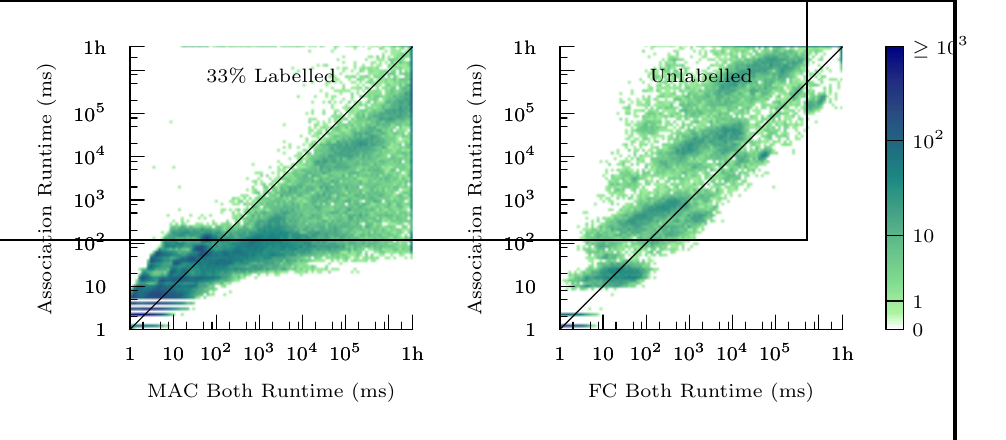
\begin{tikzpicture}[gnuplot]
%% generated with GNUPLOT 5.0p3 (Lua 5.1; terminal rev. 99, script rev. 100)
%% Fri 24 Jun 2016 20:50:33 BST
\tikzset{every node/.append style={font={\scriptsize}}}
% \path (0.000,0.000) rectangle (10.922,7.366);
\gpcolor{color=gp lt color border}
\gpsetlinetype{gp lt border}
\gpsetdashtype{gp dt solid}
\gpsetlinewidth{1.00}
\draw[gp path] (1.320,2.197)--(1.500,2.197);
\node[gp node right] at (1.136,2.197) {1};
\draw[gp path] (1.320,2.744)--(1.500,2.744);
\node[gp node right] at (1.136,2.744) {10};
\draw[gp path] (1.320,5.481)--(1.500,5.481);
\draw[gp path] (1.320,5.785)--(1.500,5.785);
\node[gp node right] at (1.136,5.785) {1h};
\draw[gp path] (1.320,2.197)--(1.500,2.197);
\draw[gp path] (1.320,2.362)--(1.410,2.362);
\draw[gp path] (1.320,2.580)--(1.410,2.580);
\draw[gp path] (1.320,2.691)--(1.410,2.691);
\draw[gp path] (1.320,2.744)--(1.500,2.744);
\draw[gp path] (1.320,2.909)--(1.410,2.909);
\draw[gp path] (1.320,3.127)--(1.410,3.127);
\draw[gp path] (1.320,3.238)--(1.410,3.238);
\draw[gp path] (1.320,3.292)--(1.500,3.292);
\node[gp node right] at (1.136,3.292) {$10^{2}$};
\draw[gp path] (1.320,3.456)--(1.410,3.456);
\draw[gp path] (1.320,3.674)--(1.410,3.674);
\draw[gp path] (1.320,3.786)--(1.410,3.786);
\draw[gp path] (1.320,3.839)--(1.500,3.839);
\node[gp node right] at (1.136,3.839) {$10^{3}$};
\draw[gp path] (1.320,4.004)--(1.410,4.004);
\draw[gp path] (1.320,4.221)--(1.410,4.221);
\draw[gp path] (1.320,4.333)--(1.410,4.333);
\draw[gp path] (1.320,4.386)--(1.500,4.386);
\node[gp node right] at (1.136,4.386) {$10^{4}$};
\draw[gp path] (1.320,4.551)--(1.410,4.551);
\draw[gp path] (1.320,4.769)--(1.410,4.769);
\draw[gp path] (1.320,4.880)--(1.410,4.880);
\draw[gp path] (1.320,4.933)--(1.500,4.933);
\node[gp node right] at (1.136,4.933) {$10^{5}$};
\draw[gp path] (1.320,5.098)--(1.410,5.098);
\draw[gp path] (1.320,5.316)--(1.410,5.316);
\draw[gp path] (1.320,5.428)--(1.410,5.428);
\draw[gp path] (1.320,5.481)--(1.500,5.481);
\draw[gp path] (1.320,5.645)--(1.410,5.645);
\draw[gp path] (1.320,2.197)--(1.320,2.377);
\node[gp node center] at (1.320,1.889) {1};
\draw[gp path] (1.867,2.197)--(1.867,2.377);
\node[gp node center] at (1.867,1.889) {10};
\draw[gp path] (4.604,2.197)--(4.604,2.377);
\draw[gp path] (4.908,2.197)--(4.908,2.377);
\node[gp node center] at (4.908,1.889) {1h};
\draw[gp path] (1.320,2.197)--(1.320,2.377);
\draw[gp path] (1.485,2.197)--(1.485,2.287);
\draw[gp path] (1.703,2.197)--(1.703,2.287);
\draw[gp path] (1.814,2.197)--(1.814,2.287);
\draw[gp path] (1.867,2.197)--(1.867,2.377);
\draw[gp path] (2.032,2.197)--(2.032,2.287);
\draw[gp path] (2.250,2.197)--(2.250,2.287);
\draw[gp path] (2.361,2.197)--(2.361,2.287);
\draw[gp path] (2.415,2.197)--(2.415,2.377);
\node[gp node center] at (2.415,1.889) {$10^{2}$};
\draw[gp path] (2.579,2.197)--(2.579,2.287);
\draw[gp path] (2.797,2.197)--(2.797,2.287);
\draw[gp path] (2.909,2.197)--(2.909,2.287);
\draw[gp path] (2.962,2.197)--(2.962,2.377);
\node[gp node center] at (2.962,1.889) {$10^{3}$};
\draw[gp path] (3.127,2.197)--(3.127,2.287);
\draw[gp path] (3.344,2.197)--(3.344,2.287);
\draw[gp path] (3.456,2.197)--(3.456,2.287);
\draw[gp path] (3.509,2.197)--(3.509,2.377);
\node[gp node center] at (3.509,1.889) {$10^{4}$};
\draw[gp path] (3.674,2.197)--(3.674,2.287);
\draw[gp path] (3.892,2.197)--(3.892,2.287);
\draw[gp path] (4.003,2.197)--(4.003,2.287);
\draw[gp path] (4.056,2.197)--(4.056,2.377);
\node[gp node center] at (4.056,1.889) {$10^{5}$};
\draw[gp path] (4.221,2.197)--(4.221,2.287);
\draw[gp path] (4.439,2.197)--(4.439,2.287);
\draw[gp path] (4.551,2.197)--(4.551,2.287);
\draw[gp path] (4.604,2.197)--(4.604,2.377);
\draw[gp path] (4.768,2.197)--(4.768,2.287);
\draw[gp path] (1.320,5.785)--(1.320,2.197)--(4.908,2.197);
\node[gp node center,rotate=-270] at (0.246,3.991) {Association Runtime (ms)};
\node[gp node center] at (3.114,1.427) {MAC Both Runtime (ms)};
\begin{scope}
\clip (1.320,5.785) rectangle (4.908,2.197);
\def\gprawrgbimagedata{%
  ffffffffffffffffffffffffffffffffffffffffffffffffffffffffffffffffffffffffffffffffffffffffffffffff%
  ffffffffffffffffff6cc78c5ab5896cc78c67c28b5ab58972cd8d5eb98a67c28b72cd8d62bd8bffffff9cea9c79d48d%
  79d48d62bd8b72cd8d9cea9c6cc78c79d48d79d48d85de9172cd8d85de9172cd8d79d48d9cea9c85de9172cd8d72cd8d%
  72cd8d79d48d72cd8d85de9172cd8dffffff85de9179d48d85de9179d48d79d48d79d48d67c28b85de9185de91ffffff%
  85de919cea9c85de91ffffff67c28b9cea9cffffffffffffffffff85de9185de91ffffffffffff9cea9c9cea9c9cea9c%
  79d48d9cea9cffffff9cea9cffffffffffff85de919cea9c85de91ffffff85de919cea9c85de9179d48d5ab58962bd8b%
  67c28b4da9874da98756b289233281ffffffffffffffffffffffffffffffffffffffffffffffffffffffffffffffffff%
  ffffffffffffffffffffffffffffffffffffffffffffffffffffffffffffffffffffffffffffffffffffffffffffffff%
  ffffffffffffffffffffffffffffffffffffffffffffffffffffffffffffffffffffffffffffffffffffffffffffffff%
  ffffffffffffffffffffffffffffffffffffffffffffffffffffffffffffffffffffffffffffffffffffffffffffffff%
  ffffffffffffffffffffffffffffffffffffffffffffffffffffffffffffffffffffffffffffffffffff9cea9cffffff%
  ffffffffffffffffffffffffffffff9cea9cffffffffffffffffffffffff9cea9cffffffffffffffffff85de919cea9c%
  ffffffffffff9cea9c9cea9cffffff9cea9c85de91ffffff85de91228b82ffffffffffffffffffffffffffffffffffff%
  ffffffffffffffffffffffffffffffffffffffffffffffffffffffffffffffffffffffffffffffffffffffffffffffff%
  ffffffffffffffffffffffffffffffffffffffffffffffffffffffffffffffffffffffffffffffffffffffffffffffff%
  ffffffffffffffffffffffffffffffffffffffffffffffffffffffffffffffffffffffffffffffffffffffffffffffff%
  ffffffffffffffffffffffffffffffffffffffffffffffffffffffffffff9cea9cffffffffffffffffffffffffffffff%
  ffffffffffff9cea9cffffffffffffffffffffffffffffffffffffffffffffffffffffffffffffffffffffffffffffff%
  ffffffffffffffffffffffffffffff9cea9cffffff9cea9c9cea9c9cea9c9cea9cffffff9cea9c85de91208a82ffffff%
  ffffffffffffffffffffffffffffffffffffffffffffffffffffffffffffffffffffffffffffffffffffffffffffffff%
  ffffffffffffffffffffffffffffffffffffffffffffffffffffffffffffffffffffffffffffffffffffffffffffffff%
  ffffffffffffffffffffffffffffffffffffffffffffffffffffffffffffffffffffffffffffffffffffffffffffffff%
  ffffffffffffffffffffffffffffffffffffffffffffffffffffffffffffffffffffffffffffffffffffffffffffffff%
  ffffffffffffffffffffffffffffffffffffffffffffffffffffffffffffffffffffffffffffffffffffffffffffffff%
  ffffffffffffffffffffffffffffffffffffffffffffffffffffff9cea9cffffffffffff9cea9c9cea9c9cea9c85de91%
  72cd8d85de9185de911e8982ffffffffffffffffffffffffffffffffffffffffffffffffffffffffffffffffffffffff%
  ffffffffffffffffffffffffffffffffffffffffffffffffffffffffffffffffffffffffffffffffffffffffffffffff%
  ffffffffffffffffffffffffffffffffffffffffffffffffffffffffffffffffffffffffffffffffffffffffffffffff%
  ffffffffffffffffffffffffffffffffffffffffffffffffffffffffffffffffffffffffffffffffffffffffffffffff%
  ffffffffffffffffffffffffffffffffffffffffffffffffffffffffffffffffffffffffffffffffffffffffffffffff%
  9cea9cffffffffffffffffffffffffffffffffffffffffffffffff9cea9c9cea9cffffff79d48dffffff85de91ffffff%
  9cea9cffffff9cea9c85de9185de9179d48d85de919cea9c1e8582ffffffffffffffffffffffffffffffffffffffffff%
  ffffffffffffffffffffffffffffffffffffffffffffffffffffffffffffffffffffffffffffffffffffffffffffffff%
  ffffffffffffffffffffffffffffffffffffffffffffffffffffffffffffffffffffffffffffffffffffffffffffffff%
  ffffffffffffffffffffffffffffffffffffffffffffffffffffffffffffffffffffffffffffffffffffffffffffffff%
  ffffffffffffffffffffffffffffffffffffffffffffffffffffffffffffffffffffffffffffffffffffffffffffffff%
  ffffffffffffffffff9cea9cffffffffffffffffffffffffffffffffffffffffffffffffffffff9cea9cffffffffffff%
  ffffff9cea9c9cea9c9cea9cffffff85de9172cd8d79d48d85de9185de9185de91ffffffffffff1f8a82ffffffffffff%
  ffffffffffffffffffffffffffffffffffffffffffffffffffffffffffffffffffffffffffffffffffffffffffffffff%
  ffffffffffffffffffffffffffffffffffffffffffffffffffffffffffffffffffffffffffffffffffffffffffffffff%
  ffffffffffffffffffffffffffffffffffffffffffffffffffffffffffffffffffffffffffffffffffffffffffffffff%
  ffffffffffffffffffffffffffffffffffffffffffffffffffffffffffffffffffffffffffffffffffffffffffffffff%
  ffffffffffffffffffffffffffffffffffffffffffffffffffffffffffff9cea9cffffffffffffffffff9cea9cffffff%
  ffffffffffffffffffffffff9cea9c9cea9cffffff9cea9cffffff9cea9cffffff67c28b9cea9c9cea9c67c28b85de91%
  85de9179d48d1f7c82ffffffffffffffffffffffffffffffffffffffffffffffffffffffffffffffffffffffffffffff%
  ffffffffffffffffffffffffffffffffffffffffffffffffffffffffffffffffffffffffffffffffffffffffffffffff%
  ffffffffffffffffffffffffffffffffffffffffffffffffffffffffffffffffffffffffffffffffffffffffffffffff%
  ffffffffffffffffffffffffffffffffffffffffffffffffffffffffffffffffffffffffffffffffffffffffffffffff%
  ffffffffffffffffffffffffffffffffffff9cea9cffffff9cea9c85de91ffffffffffffffffffffffffffffffffffff%
  ffffffffffffffffff9cea9cffffffffffff9cea9cffffffffffff9cea9cffffff9cea9c9cea9cffffffffffff79d48d%
  9cea9c6cc78c9cea9c9cea9c9cea9c9cea9c79d48d1e8982ffffffffffffffffffffffffffffffffffffffffffffffff%
  ffffffffffffffffffffffffffffffffffffffffffffffffffffffffffffffffffffffffffffffffffffffffffffffff%
  ffffffffffffffffffffffffffffffffffffffffffffffffffffffffffffffffffffffffffffffffffffffffffffffff%
  ffffffffffffffffffffffffffffffffffffffffffffffffffffffffffffffffffffffffffffffffffffffffffffffff%
  ffffffffffff9cea9cffffffffffffffffffffffffffffffffffff9cea9cffffffffffffffffffffffffffffffffffff%
  ffffffffffff9cea9cffffff9cea9c9cea9cffffffffffff9cea9cffffff9cea9c85de919cea9c85de919cea9c9cea9c%
  85de91ffffffffffffffffff9cea9c9cea9c9cea9c85de9179d48d9cea9c9cea9c9cea9c228b82ffffffffffffffffff%
  ffffffffffffffffffffffffffffffffffffffffffffffffffffffffffffffffffffffffffffffffffffffffffffffff%
  ffffffffffffffffffffffffffffffffffffffffffffffffffffffffffffffffffffffffffffffffffffffffffffffff%
  ffffffffffffffffffffffffffffffffffffffffffffffffffffffffffffffffffffffffffffffffffffffffffffffff%
  ffffffffffffffffffffffffffffffffffffffffffffffffffffff9cea9cffffffffffffffffffffffffffffffffffff%
  ffffffffffffffffffffffffffffff9cea9cffffffffffffffffff9cea9cffffffffffff9cea9cffffffffffff79d48d%
  9cea9cffffff85de9185de919cea9c9cea9c85de9185de9179d48dffffff85de9179d48dffffff79d48dffffff85de91%
  9cea9c1f7881ffffffffffffffffffffffffffffffffffffffffffffffffffffffffffffffffffffffffffffffffffff%
  ffffffffffffffffffffffffffffffffffffffffffffffffffffffffffffffffffffffffffffffffffffffffffffffff%
  ffffffffffffffffffffffffffffffffffffffffffffffffffffffffffffffffffffffffffffffffffffffffffffffff%
  ffffffffffffffffffffffffffffffffffffffffffffffffffffffffffffffffffffffffffffff9cea9cffffffffffff%
  ffffffffffffffffffffffffffffffffffffffffffffffffffffffffffff9cea9cffffffffffff9cea9cffffffffffff%
  ffffffffffffffffff9cea9cffffffffffffffffff9cea9c9cea9c9cea9c9cea9c85de9185de919cea9c72cd8d67c28b%
  79d48dffffff79d48d79d48d6cc78c79d48d1f7481ffffffffffffffffffffffffffffffffffffffffffffffffffffff%
  ffffffffffffffffffffffffffffffffffffffffffffffffffffffffffffffffffffffffffffffffffffffffffffffff%
  ffffffffffffffffffffffffffffffffffffffffffffffffffffffffffffffffffffffffffffffffffffffffffffffff%
  ffffffffffffffffffffffffffffffffffffffffffffffffffffffffffffffffffffffffffffffffffffffffffffffff%
  ffffffffffffffffffffffffffffffffffffffffffffffffffffffffffffffffffffffffffffffffffff9cea9c9cea9c%
  9cea9cffffffffffffffffff85de919cea9c85de9185de91ffffff85de9185de9172cd8d9cea9cffffff79d48d85de91%
  85de9172cd8dffffff79d48dffffff72cd8d9cea9cffffffffffff72cd8d79d48d1f7381ffffffffffffffffffffffff%
  ffffffffffffffffffffffffffffffffffffffffffffffffffffffffffffffffffffffffffffffffffffffffffffffff%
  ffffffffffffffffffffffffffffffffffffffffffffffffffffffffffffffffffffffffffffffffffffffffffffffff%
  ffffffffffffffffffffffffffffffffffffffffffffffffffffffffffffffffffffffffffffffffffffffffffffffff%
  ffffffffffffffffffffffffffffffffffffffffffffffffffffffffffffffffffffffffffffffffffffffffffffffff%
  ffffffffffffffffffffffffffffff9cea9c9cea9cffffffffffffffffff9cea9cffffffffffff85de9185de919cea9c%
  ffffff9cea9c79d48dffffff9cea9c79d48d9cea9c79d48d9cea9c85de916cc78c9cea9c72cd8d6cc78c72cd8d72cd8d%
  216881ffffffffffffffffffffffffffffffffffffffffffffffffffffffffffffffffffffffffffffffffffffffffff%
  ffffffffffffffffffffffffffffffffffffffffffffffffffffffffffffffffffffffffffffffffffffffffffffffff%
  ffffffffffffffffffffffffffffffffffffffffffffffffffffffffffffffffffffffffffffffffffffffffffffffff%
  ffffffffffffffffffffffffffffffffffffffffffffffffffffffffffffffffffffffffffffffffffffffffffffffff%
  ffffffffffff9cea9cffffffffffffffffffffffff9cea9c9cea9cffffff9cea9cffffff9cea9cffffffffffffffffff%
  9cea9c9cea9cffffff9cea9cffffff9cea9c79d48d85de919cea9c85de919cea9c9cea9c85de919cea9c9cea9c85de91%
  85de9179d48d85de9172cd8d9cea9c206e81ffffffffffffffffffffffffffffffffffffffffffffffffffffffffffff%
  ffffffffffffffffffffffffffffffffffffffffffffffffffffffffffffffffffffffffffffffffffffffffffffffff%
  ffffffffffffffffffffffffffffffffffffffffffffffffffffffffffffffffffffffffffffffffffffffffffffffff%
  ffffffffffffffffffffffffffffffffffffffffffffffffffffffffffffffffffffffffffffffffffffffffffffffff%
  ffffffffffffffffffffffff9cea9cffffffffffffffffffffffffffffffffffffffffff9cea9cffffffffffffffffff%
  ffffffffffff9cea9cffffffffffffffffffffffff9cea9cffffff9cea9cffffffffffff9cea9c79d48d9cea9c9cea9c%
  ffffff85de9172cd8d9cea9c85de919cea9c6cc78c9cea9c6cc78c53af88206e81ffffffffffffffffffffffffffffff%
  ffffffffffffffffffffffffffffffffffffffffffffffffffffffffffffffffffffffffffffffffffffffffffffffff%
  ffffffffffffffffffffffffffffffffffffffffffffffffffffffffffffffffffffffffffffffffffffffffffffffff%
  ffffffffffffffffffffffffffffffffffffffffffffffffffffffffffffffffffffffffffffffffffffffffffffffff%
  ffffffffffffffffffffffffffffffffffffffffffffffffffffffffffffffffffffffffffffffffffffffffffffffff%
  ffffffffffffffffff9cea9cffffffffffffffffff85de91ffffffffffff9cea9c9cea9c9cea9c85de91ffffff72cd8d%
  9cea9cffffffffffff85de91ffffff85de9185de919cea9c72cd8d72cd8dffffff79d48d62bd8b5eb98a72cd8d206a81%
  ffffffffffffffffffffffffffffffffffffffffffffffffffffffffffffffffffffffffffffffffffffffffffffffff%
  ffffffffffffffffffffffffffffffffffffffffffffffffffffffffffffffffffffffffffffffffffffffffffffffff%
  ffffffffffffffffffffffffffffffffffffffffffffffffffffffffffffffffffffffffffffffffffffffffffffffff%
  ffffffffffffffffffffffffffffffffffffffffffffffffffffffffffffffffffffffffffffffffffffffffffffffff%
  ffffffffffffffffffffffff9cea9cffffffffffffffffffffffff9cea9c9cea9c9cea9c9cea9c9cea9c9cea9cffffff%
  ffffff9cea9cffffff9cea9cffffff85de919cea9c85de9185de919cea9cffffff85de9185de9167c28b79d48d85de91%
  79d48d62bd8b62bd8b5ab589216881ffffffffffffffffffffffffffffffffffffffffffffffffffffffffffffffffff%
  ffffffffffffffffffffffffffffffffffffffffffffffffffffffffffffffffffffffffffffffffffffffffffffffff%
  ffffffffffffffffffffffffffffffffffffffffffffffffffffffffffffffffffffffffffffffffffffffffffffffff%
  ffffffffffffffffffffffffffffffffffffffffffffffffffffffffffffffffffffffffffffffffffffffffffffffff%
  ffffffffffffffffffffffffffffffffffffffffffffffffffffffffffffffffff9cea9cffffffffffffffffffffffff%
  9cea9cffffffffffffffffff85de91ffffff9cea9cffffffffffff9cea9c85de9185de9185de9185de9185de91ffffff%
  85de9179d48d72cd8d79d48d79d48d62bd8b67c28b3b9c854da987216781ffffffffffffffffffffffffffffffffffff%
  ffffffffffffffffffffffffffffffffffffffffffffffffffffffffffffffffffffffffffffffffffffffffffffffff%
  ffffffffffffffffffffffffffffffffffffffffffffffffffffffffffffffffffffffffffffffffffffffffffffffff%
  ffffffffffffffffffffffffffffffffffffffffffffffffffffffffffffffffffffffffffffffffffffffffffffffff%
  ffffffffffffffffffffffffffffffffffff9cea9cffffffffffffffffffffffffffffff9cea9cffffffffffffffffff%
  9cea9cffffff9cea9c9cea9cffffffffffffffffffffffffffffff85de91ffffffffffff72cd8d85de919cea9c79d48d%
  9cea9c79d48d72cd8d85de9185de9185de9172cd8d79d48d5ab5896cc78c5ab58956b28950ac8850ac88226281ffffff%
  ffffffffffffffffffffffffffffffffffffffffffffffffffffffffffffffffffffffffffffffffffffffffffffffff%
  ffffffffffffffffffffffffffffffffffffffffffffffffffffffffffffffffffffffffffffffffffffffffffffffff%
  ffffffffffffffffffffffffffffffffffffffffffffffffffffffffffffffffffffffffffffffffffffffffffffffff%
  ffffffffffffffffffffffffffffffffffffffffffffffffffffffffffffffffffffffffffffffffffffffffffffffff%
  ffffffffffffffffffffffffffffffffffffffffff9cea9cffffffffffffffffff9cea9cffffffffffff9cea9cffffff%
  ffffffffffffffffffffffff85de9185de9172cd8d85de91ffffff9cea9c79d48d67c28b6cc78c6cc78c53af8856b289%
  53af883e9d854da987206b81ffffffffffffffffffffffffffffffffffffffffffffffffffffffffffffffffffffffff%
  ffffffffffffffffffffffffffffffffffffffffffffffffffffffffffffffffffffffffffffffffffffffffffffffff%
  ffffffffffffffffffffffffffffffffffffffffffffffffffffffffffffffffffffffffffffffffffffffffffffffff%
  ffffffffffffffffffffffffffffffffffffffffffffffffffffffffffffffffffffffffffffffffffffffffffffffff%
  ffffffffffffffffffffffffffffff9cea9cffffffffffffffffff9cea9cffffff79d48dffffff9cea9cffffff9cea9c%
  ffffffffffff79d48dffffff9cea9c9cea9c85de91ffffff9cea9c72cd8dffffff79d48d9cea9c9cea9c9cea9c5eb98a%
  5ab58967c28b53af8853af88409f864aa78753af8845a286226481ffffffffffffffffffffffffffffffffffffffffff%
  ffffffffffffffffffffffffffffffffffffffffffffffffffffffffffffffffffffffffffffffffffffffffffffffff%
  ffffffffffffffffffffffffffffffffffffffffffffffffffffffffffffffffffffffffffffffffffffffffffffffff%
  ffffffffffffffffffffffffffffffffffffffffffffffffffffffffffffffffffffffffffffffffffffffffffffffff%
  ffffffffffffffffffffffffffffffffffffffffffffffffffffffffffffffffffffffffffffffffffffffffffffffff%
  ffffff9cea9cffffffffffffffffffffffff9cea9cffffffffffff9cea9c9cea9c79d48d9cea9c85de91ffffff85de91%
  85de9185de9179d48d67c28b72cd8d79d48d5ab58956b28956b2894aa78750ac8856b28943a186206e81ffffffffffff%
  ffffffffffffffffffffffffffffffffffffffffffffffffffffffffffffffffffffffffffffffffffffffffffffffff%
  ffffffffffffffffffffffffffffffffffffffffffffffffffffffffffffffffffffffffffffffffffffffffffffffff%
  ffffffffffffffffffffffffffffffffffffffffffffffffffffffffffffffffffffffffffffffffffffffffffffffff%
  ffffffffffffffffffffffffffffffffffffffffffffffffffffffffffffffffffffffffffffffffffffffffffffffff%
  ffffffffffffffffffffffffffffffffffff9cea9cffffffffffffffffff9cea9c9cea9c85de9185de919cea9c9cea9c%
  ffffffffffff85de9185de9185de919cea9c85de9179d48d5ab58972cd8d67c28b56b28953af885ab58931958453af88%
  43a1865ab589206981ffffffffffffffffffffffffffffffffffffffffffffffffffffffffffffffffffffffffffffff%
  ffffffffffffffffffffffffffffffffffffffffffffffffffffffffffffffffffffffffffffffffffffffffffffffff%
  ffffffffffffffffffffffffffffffffffffffffffffffffffffffffffffffffffffffffffffffffffffffffffffffff%
  ffffffffffffffffffffffffffffffffffffffffffffffffffffffffffffffffffffffffffffffffffffffffffffffff%
  ffffffffffffffffffffffff9cea9cffffffffffffffffff9cea9cffffffffffffffffff9cea9c9cea9cffffffffffff%
  9cea9c9cea9c85de919cea9c9cea9c79d48d72cd8d79d48d9cea9c79d48d6cc78c79d48d72cd8d6cc78c48a5864aa787%
  48a586409f864aa7873e9d8543a18653af884da987206b81ffffffffffffffffffffffffffffffffffffffffffffffff%
  ffffffffffffffffffffffffffffffffffffffffffffffffffffffffffffffffffffffffffffffffffffffffffffffff%
  ffffffffffffffffffffffffffffffffffffffffffffffffffffffffffffffffffffffffffffffffffffffffffffffff%
  ffffffffffffffffffffffffffffffffffffffffffffffffffffffffffffffffffffffffffffffffffffffffffffffff%
  ffffffffffffffffffffffffffffffffffffffffff9cea9cffffff9cea9cffffffffffffffffff85de91ffffffffffff%
  ffffff79d48dffffff9cea9cffffffffffff9cea9c9cea9c9cea9c72cd8d85de9172cd8d9cea9c72cd8d6cc78c62bd8b%
  67c28b50ac8850ac8850ac8848a58650ac8848a58656b28943a18650ac884aa78767c28b1f7881ffffffffffffffffff%
  ffffffffffffffffffffffffffffffffffffffffffffffffffffffffffffffffffffffffffffffffffffffffffffffff%
  ffffffffffffffffffffffffffffffffffffffffffffffffffffffffffffffffffffffffffffffffffffffffffffffff%
  ffffffffffffffffffffffffffffffffffffffffffffffffffffffffffffffffffffffffffffffffffffffffffffffff%
  ffffffffffffffffffffffffffffffffffffffffffffffffffffffffffffffffffffffffffffffffffffffffffffffff%
  ffffffffffffffffffffffffffffff85de919cea9c79d48d9cea9c9cea9cffffff9cea9cffffff85de9167c28b79d48d%
  5eb98a9cea9c62bd8b62bd8b53af8856b2894da98750ac885eb98a53af884da98753af8843a186409f8653af885ab589%
  56b2891e8282ffffffffffffffffffffffffffffffffffffffffffffffffffffffffffffffffffffffffffffffffffff%
  ffffffffffffffffffffffffffffffffffffffffffffffffffffffffffffffffffffffffffffffffffffffffffffffff%
  ffffffffffffffffffffffffffffffffffffffffffffffffffffffffffffffffffffffffffffffffffffffffffffffff%
  ffffffffffffffffffffffffffffffffffffffffffffffffffffffffffffffffffffffffffffffffffffffffffffffff%
  ffffffffffff9cea9c9cea9c9cea9cffffffffffffffffffffffff9cea9cffffff85de919cea9c9cea9c85de9179d48d%
  ffffff79d48d9cea9c72cd8d6cc78c79d48d6cc78c5ab5896cc78c6cc78c5eb98a43a1864aa7874da987409f863e9d85%
  50ac885eb98a5ab58953af8867c28b6cc78c248d83ffffffffffffffffffffffffffffffffffffffffffffffffffffff%
  ffffffffffffffffffffffffffffffffffff9cea9cffffffffffffffffffffffffffffffffffffffffffffffffffffff%
  ffffffffffffffffffffffffffffffffffffffffffffffffffffffffffffffffffffffffffffffffffffffffffffffff%
  ffffffffffffffffffffffffffffffffffffffffffffffffffffffffffffffffffffffffffffffffffffffffffffffff%
  ffffffffffffffffffffffffffffffffffffffffff85de91ffffffffffff9cea9cffffff9cea9cffffff9cea9cffffff%
  9cea9c85de9179d48dffffffffffff72cd8d9cea9c79d48d79d48d79d48d79d48d79d48d85de9167c28b6cc78c53af88%
  62bd8b72cd8d53af8856b2895eb98a62bd8b72cd8d6cc78c6cc78c79d48d85de911e8482ffffffffffffffffffffffff%
  ffffffffffffffffffffffffffffffffffffffffffffffffffffffffffffffffffffffffffffffffffffffffffffffff%
  ffffffffffffffffffffffffffffffffffffffffffffffffffffffffffffffffffffffffffffffffffffffffffffffff%
  ffffffffffffffffffffffffffffffffffffffffffffffffffffffffffffffffffffffffffffffffffffffffffffffff%
  ffffffffffffffffff9cea9cffffffffffffffffffffffffffffffffffffffffffffffffffffffffffff85de919cea9c%
  ffffff9cea9c9cea9cffffffffffffffffff79d48d85de9172cd8d79d48d85de916cc78c9cea9c79d48d72cd8d9cea9c%
  67c28b67c28b72cd8d72cd8d56b2896cc78c5ab58962bd8b5eb98a85de9179d48d67c28b6cc78c85de9172cd8d72cd8d%
  208a82ffffffffffffffffffffffffffffffffffffffffffffffffffffffffffffffffffffffffffffffffffffffffff%
  ffffffffffffffffffffffffffffffffffffffffffffffffffffffffffffffffffffffffffffffffffffffffffffffff%
  ffffffffffffffffffffffffffffffffffffffffffffffffffffffffffffffffffffffffffffffffffffffffffffffff%
  ffffffffffffffffffffffffffffffffffffffffffffffffffffffffffffffffffffffffffffffffffffffffffffffff%
  ffffff9cea9cffffff9cea9cffffff9cea9c85de919cea9c9cea9c85de9179d48d6cc78c85de919cea9c72cd8d9cea9c%
  79d48d79d48d85de916cc78c72cd8d67c28b53af885ab5894da98779d48d72cd8d6cc78c67c28b79d48d85de9179d48d%
  ffffff72cd8d9cea9c9cea9c9cea9c2e9384ffffffffffffffffffffffffffffffffffffffffffffffffffffffffffff%
  ffffffffffffffffffffffffffffffffffffffffffffffffffffffffffffffffffffffffffffffffffffffffffffffff%
  ffffffffffffffffffffffffffffffffffffffffffffffffffffffffffffffffffffffffffffffffffffffffffffffff%
  ffffffffffffffffffffffffffffffffffffffffffffffffffffffffffffffffffffffffffffffffffffffffffffffff%
  ffffffffffffffffffffffffffffffffffff9cea9c9cea9cffffff9cea9c9cea9cffffff72cd8dffffff85de9179d48d%
  72cd8d85de919cea9c9cea9c85de916cc78c62bd8b85de9167c28b67c28b5eb98a5ab58950ac8867c28b53af8853af88%
  79d48d72cd8d85de916cc78cffffff85de9185de9185de919cea9cffffff1e8582ffffffffffffffffffffffffffffff%
  ffffffffffffffffffffffffffffffffffffffffffffffffffffffffffffffffffffffffffffffffffffffffffffffff%
  ffffffffffffffffffffffffffffffffffffffffffffffffffffffffffffffffffffffffffffffffffffffffffffffff%
  ffffffffffffffffffffffffffffffffffffffffffffffffffffffffffffffffffffffffffffffffffffffffffffffff%
  ffffffffffffffffffffffffffffffffffffffffffffffffffffffffffffffffff9cea9cffffff9cea9c85de9185de91%
  ffffff85de9179d48d85de919cea9c9cea9c79d48d72cd8d85de9185de916cc78c53af8856b28950ac885eb98a45a286%
  53af885ab5896cc78c67c28b62bd8b56b2896cc78c85de9185de916cc78c72cd8d85de9172cd8dffffff85de91319584%
  ffffffffffffffffffffffffffffffffffffffffffffffffffffffffffffffffffffffffffffffffffffffffffffffff%
  ffffffffffffffffffffffffffffffffffffffffffffffffffffffffffffffffffffffffffffffffffffffffffffffff%
  ffffffffffffffffffffffffffffffffffffffffffffffffffffffffffffffffffffffffffffffffffffffffffffffff%
  ffffffffffffffffffffffffffffffffffffffffffffffffffffffffffffffffffffffffffffff9cea9cffffffffffff%
  ffffff9cea9c9cea9c9cea9cffffff9cea9cffffff9cea9c85de9167c28b72cd8d79d48d72cd8d6cc78c72cd8d72cd8d%
  50ac8867c28b4da9876cc78c62bd8b50ac8845a28645a2865ab58967c28b85de916cc78c79d48d85de9179d48d9cea9c%
  9cea9c72cd8d79d48d85de91268e83ffffffffffffffffffffffffffffffffffffffffffffffffffffffffffffffffff%
  ffffffffffffffffffffffffffffffffffffffffffffffffffffffffffffffffffffffffffffffffffffffffffffffff%
  ffffffffffffffffffffffffffffffffffffffffffffffffffffffffffffffffffffffffffffffffffffffffffffffff%
  ffffffffffffffffffffffffffffffffffffffffffffffffffffffffffffffffffffffffffffffffffffffffffffffff%
  ffffffffffffffffffffffff85de91ffffffffffffffffff9cea9c9cea9c9cea9c85de9185de9179d48d72cd8d85de91%
  72cd8d5eb98a72cd8d53af885eb98a56b2894aa7874da98753af8843a18650ac883e9d855ab58953af885ab58962bd8b%
  72cd8d79d48d72cd8d79d48d9cea9cffffff9cea9c9cea9c85de912a9183ffffffffffffffffffffffffffffffffffff%
  ffffffffffffffffffffffffffffffffffffffffffffffffffffffffffffffffffffffffffffffffffffffffffffffff%
  ffffffffffffffffffffffffffffffffffffffffffffffffffffffffffffffffffffffffffffffffffffffffffffffff%
  ffffffffffffffffffffffffffffffffffffffffffffffffffffffffffffffffffffffffffffffffffffffffffffffff%
  ffffff9cea9cffffffffffffffffffffffffffffffffffffffffff9cea9cffffff9cea9c85de91ffffff9cea9c9cea9c%
  72cd8d62bd8b85de9185de9145a28662bd8b53af8850ac885eb98a48a58645a2863e9d853799853b9c85409f864da987%
  4aa7875ab5894da9875ab58956b2896cc78c72cd8d85de9179d48d9cea9c9cea9c9cea9c79d48d9cea9c248d83ffffff%
  ffffffffffffffffffffffffffffffffffffffffffffffffffffffffffffffffffffffffffffffffffffffffffffffff%
  ffffffffffffffffffffffffffffffffffffffffffffffffffffffffffffffffffffffffffffffffffffffffffffffff%
  ffffffffffffffffffffffffffffffffffffffffffffffffffffffffffffffffffffffffffffffffffffffffffffffff%
  ffffffffffffffffffffffffffffffffffffffffffffffff9cea9cffffffffffffffffffffffff9cea9cffffff9cea9c%
  79d48d9cea9c9cea9c5eb98a6cc78c5eb98a53af885ab5894aa78750ac8845a2865ab589409f8656b28945a28643a186%
  3e9d852e9384399a8535988456b289409f8648a5865ab58956b28967c28b72cd8d72cd8d9cea9c85de9185de9172cd8d%
  ffffff72cd8d6cc78c2c9283ffffffffffffffffffffffffffffffffffffffffffffffffffffffffffffffffffffffff%
  ffffffffffffffffffffffffffffffffffffffffffffffffffffffffffffffffffffffffffffffffffffffffffffffff%
  ffffffffffffffffffffffffffffffffffffffffffffffffffffffffffffffffffffffffffffffffffffffffffffffff%
  ffffffffffffffffffffffffffffffffffffffffffffffffffffffffffffffffff9cea9cffffff9cea9cffffffffffff%
  9cea9cffffffffffffffffff9cea9c9cea9c9cea9c79d48d79d48d67c28b72cd8d5eb98a45a28662bd8b43a1864aa787%
  4aa78743a18643a1864da9873b9c8548a586409f8650ac8848a5864da98756b28962bd8b67c28b72cd8d50ac886cc78c%
  9cea9c9cea9c85de919cea9c79d48d85de9179d48d6cc78c409f86ffffffffffffffffffffffffffffffffffffffffff%
  ffffffffffffffffffffffffffffffffffffffffffffffffffffffffffffffffffffffffffffffffffffffffffffffff%
  ffffffffffffffffffffffffffffffffffffffffffffffffffffffffffffffffffffffffffffffffffffffffffffffff%
  ffffffffffffffffffffffffffffffffffffffffffffffffffffffffffffffffffffffffffffffffffff9cea9cffffff%
  ffffffffffffffffffffffffffffffffffffffffff85de919cea9cffffffffffff6cc78c72cd8d67c28b6cc78c67c28b%
  5ab5894aa78753af8856b2894da98745a2864aa78743a186409f8648a58650ac8853af884aa78750ac8853af8856b289%
  5ab5896cc78c67c28b85de9172cd8d79d48d85de919cea9c79d48d79d48d9cea9c85de919cea9c2f9484ffffffffffff%
  ffffffffffffffffffffffffffffffffffffffffffffffffffffffffffffffffffffffffffffffffffffffffffffffff%
  ffffffffffffffffffffffffffffffffffffffffffffffffffffffffffffffffffffffffffffffffffffffffffffffff%
  ffffffffffffffffffffffffffffffffffffffffffffffffffffffffffffffffffffffffffffffffffffffffffffffff%
  ffffffffffffffffffffffffffffff9cea9cffffffffffffffffffffffff9cea9c9cea9cffffff85de916cc78cffffff%
  6cc78c79d48d72cd8d62bd8b67c28b5eb98a5eb98a48a5864da987409f864aa7874aa78745a28653af884da9874aa787%
  62bd8b56b28953af885eb98a62bd8b72cd8d79d48d67c28b79d48d79d48d85de9185de9185de9172cd8d72cd8d62bd8b%
  6cc78c79d48d278f83ffffffffffffffffffffffffffffffffffffffffffffffffffffffffffffffffffffffffffffff%
  ffffffffffffffffffffffffffffffffffffffffffffffffffffffffffffffffffffffffffffffffffffffffffffffff%
  ffffffffffffffffffffffffffffffffffffffffffffffffffffffffffffffffffffffffffffffffffffffffffffffff%
  ffffffffffffffffffffffffffffffffffffffffffffffffffffffffffffffffffffffffffffffffffff9cea9c9cea9c%
  9cea9cffffff9cea9c85de9172cd8d79d48d6cc78c5eb98a5ab58967c28b45a2864da98753af8850ac884da9874aa787%
  45a28645a28645a2865ab58950ac8872cd8d50ac8867c28b5ab5896cc78c72cd8d62bd8b72cd8d79d48d85de91ffffff%
  6cc78c72cd8d85de919cea9c85de916cc78c85de91379985ffffffffffffffffffffffffffffffffffffffffffffffff%
  ffffffffffffffffffffffffffffffffffffffffffffffffffffffffffffffffffffffffffffffffffffffffffffffff%
  ffffffffffffffffffffffffffffffffffffffffffffffffffffffffffffffffffffffffffffffffffffffffffffffff%
  ffffffffffffffffffffffffffffffffffffffffffffffffffffffffffffffffffffffffffffffffffffffffffffffff%
  ffffff9cea9cffffffffffff9cea9c79d48d9cea9c9cea9c79d48d6cc78c6cc78c67c28b5eb98a4aa78753af8856b289%
  4da98750ac886cc78c4aa78772cd8d67c28b4aa7875ab58962bd8b72cd8d62bd8b5ab5896cc78c5ab58967c28b6cc78c%
  79d48d79d48d79d48d79d48d79d48d6cc78c6cc78c79d48d6cc78c79d48d79d48d85de912e9384ffffffffffffffffff%
  ffffffffffffffffffffffffffffffffffffffffffffffffffffffffffffffffffffffffffffffffffffffffffffffff%
  ffffffffffffffffffffffffffffffffffffffffffffffffffffffffffffffffffffffffffffffffffffffffffffffff%
  ffffffffffffffffffffffffffffffffffffffffffffffffffffffffffffffffffffffffffffffffffffffffffffffff%
  ffffffffffff9cea9cffffffffffffffffffffffffffffffffffff85de9179d48dffffff79d48d85de916cc78c53af88%
  3e9d855ab5893e9d8545a2865eb98a4da98748a5865eb98a53af8862bd8b62bd8b67c28b67c28b6cc78c5eb98a79d48d%
  67c28b67c28b72cd8d6cc78c6cc78c79d48d62bd8b62bd8b72cd8d72cd8d85de916cc78c79d48d62bd8bffffff79d48d%
  79d48d1e8582ffffffffffffffffffffffffffffffffffffffffffffffffffffffffffffffffffffffffffffffffffff%
  ffffffffffffffffffffffffffffffffffffffffffffffffffffffffffffffffffffffffffffffffffffffffffffffff%
  ffffffffffffffffffffffffffffffffffffffffffffffffffffffffffffffffffffffffffffffffffff9cea9cffffff%
  ffffffffffffffffffffffffffffffffffffffffffffffff9cea9cffffffffffffffffff85de9185de919cea9c9cea9c%
  85de9179d48d85de9172cd8d53af8850ac8850ac884da9875eb98a5eb98a62bd8b62bd8b50ac8856b28956b2895eb98a%
  67c28b6cc78c5eb98a62bd8b6cc78c62bd8b62bd8b6cc78c85de915eb98a72cd8d72cd8d72cd8d79d48d85de9179d48d%
  85de9172cd8d79d48d79d48d85de9185de91319584ffffffffffffffffffffffffffffffffffffffffffffffffffffff%
  9cea9cffffffffffffffffffffffffffffffffffff9cea9cffffffffffffffffffffffffffffffffffffffffffffffff%
  ffffffffffffffffffffffffffffffffffffffffffffffffffffffffffffffffffffffffffffffffffffffffffffffff%
  ffffffffffffffffffffffffffffffffffffffffffffffffffffff9cea9cffffffffffff9cea9cffffff85de919cea9c%
  9cea9c85de91ffffff9cea9c9cea9c9cea9c85de9172cd8d6cc78c67c28b79d48d43a1865ab58956b28956b28962bd8b%
  4da98750ac8853af8856b28950ac8856b2896cc78c67c28b79d48d85de9172cd8d79d48d72cd8d62bd8b72cd8d67c28b%
  72cd8d9cea9c85de919cea9c9cea9c79d48d79d48d79d48d72cd8d79d48d9cea9c359884ffffffffffffffffffffffff%
  ffffffffffffffffffffffffffffffffffffffffffffffffffffffffffffffffffffffffffffffffffffffffffffffff%
  ffffffffffffffffffffffffffffffffffffffffffffffffffffffffffffffffffffffffffffffffffffffffffffffff%
  ffffffffffffffffffffffffffffffffffffffffffffffffffffffffffffffffffffffffffffffffffffffffffffffff%
  ffffff9cea9c9cea9c9cea9cffffffffffff9cea9c72cd8d85de9172cd8d5eb98a6cc78c6cc78c67c28b62bd8b72cd8d%
  4da98767c28b5eb98a4aa78762bd8b67c28b5eb98a67c28b5eb98a62bd8b72cd8d67c28b72cd8d9cea9c72cd8d62bd8b%
  79d48d5eb98a6cc78c5eb98a5eb98a67c28b72cd8d9cea9c9cea9c62bd8b6cc78cffffff79d48d79d48d85de9179d48d%
  2c9283ffffffffffffffffffffffffffffffffffffffffffffffffffffffffffffffffffffffffffffffffffffffffff%
  ffffffffffffffffffffffffffffffffffffffffffffffffffffffffffffffffffffffffffffffffffffffffffffffff%
  ffffffffffffffffffffffffffffffffffffffffffffffffffffffffffffffffffffffffffffffffffff9cea9c9cea9c%
  9cea9cffffffffffffffffff9cea9cffffff9cea9cffffff9cea9c85de919cea9c72cd8d6cc78c79d48d79d48d79d48d%
  62bd8b56b2896cc78c62bd8b67c28b67c28b4aa7875eb98a67c28b79d48d72cd8d79d48d72cd8d72cd8d79d48d5eb98a%
  5ab5895ab5895eb98a72cd8d79d48d79d48d85de9167c28b6cc78c67c28b67c28b6cc78c9cea9c79d48d79d48d85de91%
  72cd8d85de91ffffff9cea9c79d48d268e83ffffffffffffffffffffffffffffffffffffffffffffffffffffffffffff%
  ffffffffffffffffffffffffffffffffffffffffffffffffffffffffffffffffffffffffffffffffffffffffffffffff%
  ffffffffffffffffffffffffffffffffffffffffffffffffffffffffffffffffffffffffffffffffffffffffffffffff%
  ffffffffffffffffffffffffffffff85de91ffffff85de91ffffffffffffffffff9cea9cffffff85de919cea9c85de91%
  85de916cc78c6cc78c72cd8d5eb98a5ab5899cea9c56b28962bd8b62bd8b72cd8d85de9185de9167c28b67c28b72cd8d%
  72cd8d79d48d53af889cea9c62bd8b72cd8d9cea9c67c28b79d48d6cc78c67c28b72cd8d67c28b72cd8d5eb98a9cea9c%
  72cd8d72cd8d62bd8b72cd8d85de9179d48d9cea9c85de919cea9c6cc78c2e9384ffffffffffffffffffffffffffffff%
  ffffffffffffffffffffffffffffffffffffffffffffffffffffffffffffffffffffffffffffffffffffffffffffffff%
  ffffffffffffffffffffffffffffffffffffffffffffffffffffffffffffffffffffffffffffffffffffffffffffffff%
  ffffffffffffffffffffffffffffff9cea9cffffffffffffffffff9cea9cffffffffffffffffff9cea9cffffff9cea9c%
  9cea9c6cc78c79d48d72cd8d79d48d85de9185de916cc78c67c28b5eb98a67c28b62bd8b67c28b9cea9c79d48d5ab589%
  79d48d67c28b6cc78c79d48d67c28b67c28b67c28b6cc78c67c28b72cd8d72cd8d62bd8b85de919cea9c85de9185de91%
  72cd8d79d48d6cc78c79d48d62bd8b72cd8d5ab5896cc78c79d48d6cc78c79d48d9cea9c6cc78c85de919cea9c2c9283%
  ffffffffffffffffffffffffffffffffffffffffffffffffffffffffffffffffffffffffffffffffffffffffffffffff%
  ffffffffffffffffffffffffffffffffffffffffffffffffffffffffffffffffffffffffffffffffffffffffffffffff%
  ffffffffffffffffffffffffffffffffffffffffffffffffffffffffffffffffffffffff9cea9c85de91ffffff9cea9c%
  ffffffffffffffffff85de919cea9c9cea9cffffff9cea9c72cd8d6cc78c85de9172cd8d72cd8d67c28b62bd8b62bd8b%
  72cd8d5ab5896cc78c67c28b5ab58967c28b72cd8d6cc78c4aa78767c28b56b2899cea9c6cc78c79d48d6cc78c72cd8d%
  79d48d72cd8d62bd8b85de9185de916cc78c72cd8d85de9172cd8d72cd8d79d48d6cc78c6cc78c79d48d79d48d85de91%
  79d48d85de9167c28b85de912e9384ffffffffffffffffffffffffffffffffffffffffffffffffffffffffffffffffff%
  ffffffffffffffffffffffffffffffffffffffffffffffffffffffffffffffffffffffffffffffffffffffffffffffff%
  ffffffffffffffffffffffffffffffffffffffffffffffffffffffffffffffffffffffffffffffffffffffffffffffff%
  ffffffffffff9cea9cffffff9cea9c79d48dffffff85de919cea9cffffff9cea9c85de9172cd8d79d48d9cea9c72cd8d%
  79d48d5eb98a5eb98a62bd8b79d48d72cd8d79d48d72cd8d67c28b6cc78c53af8862bd8b5eb98a9cea9c5ab58967c28b%
  67c28b67c28b6cc78c67c28b6cc78c72cd8d72cd8d62bd8b79d48d6cc78c6cc78c72cd8d6cc78c67c28b72cd8d79d48d%
  79d48d79d48d79d48d9cea9c79d48d72cd8d9cea9c6cc78cffffff43a186ffffffffffffffffffffffffffffffffffff%
  ffffffffffffffffffffffffffffffffffffffffffffffffffffffffffffffffffffffff9cea9cffffffffffffffffff%
  ffffffffffffffffffffffffffffffffffffffffffffffffffffffffffffffffffffffffffffffffffffffffffffffff%
  ffffffffffffffffffffffffffffffffffff85de91ffffffffffffffffff79d48d79d48dffffff6cc78c85de919cea9c%
  62bd8b79d48d67c28b53af8862bd8b53af885eb98a50ac8879d48d5eb98a5eb98a5eb98a6cc78c79d48d48a58667c28b%
  4aa7875eb98a53af886cc78c5ab5896cc78c72cd8d50ac8872cd8d62bd8b6cc78c5ab589ffffff85de9172cd8d6cc78c%
  67c28b62bd8b79d48d79d48d72cd8d79d48d72cd8d85de9167c28b6cc78c85de9185de9172cd8d9cea9c43a186ffffff%
  ffffffffffffffffffffffffffffffffffffffffffffffffffffffffffffffffffffffffffffffffffffffffffffffff%
  ffffffffffffffffffffffffffffffffffffffffffffffffffffffffffffffffffffffffffffffffffffffffffffffff%
  ffffffffffffffffffffffffffffffffffffffffffffffffffffff9cea9cffffff9cea9c85de91ffffffffffff9cea9c%
  79d48dffffff79d48d72cd8d9cea9c5eb98a62bd8b79d48d4da98756b28953af886cc78c6cc78c6cc78c5ab58962bd8b%
  5ab58972cd8d85de9167c28b6cc78c50ac8856b2896cc78c62bd8b67c28b67c28b85de9162bd8b6cc78c67c28b6cc78c%
  72cd8d6cc78c79d48d85de9179d48d5ab58985de916cc78c85de9167c28b9cea9c79d48d79d48d72cd8d72cd8dffffff%
  9cea9c9cea9c85de912f9484ffffffffffffffffffffffffffffffffffffffffffffffffffffffffffffffffffffffff%
  ffffffffffffffffffffffffffffffffffffffffffffffffffffffffffffffffffffffffffffffffffffffffffffffff%
  ffffffffffffffffffffffffffffffffffffffffffffffffffffffffffffffffffffffffffffffffffffffffffffffff%
  9cea9c79d48d6cc78cffffff79d48d79d48d79d48d9cea9c6cc78c6cc78c67c28b56b2895eb98a53af8862bd8b5ab589%
  67c28b62bd8b67c28b62bd8b6cc78c9cea9c6cc78c5eb98a79d48d50ac8862bd8b5eb98a5ab58962bd8b62bd8b6cc78c%
  6cc78c9cea9c5eb98a72cd8d6cc78c72cd8d5eb98a9cea9c6cc78c67c28b6cc78c62bd8b62bd8b6cc78c6cc78c79d48d%
  85de9172cd8d9cea9cffffff9cea9c79d48d6cc78c79d48d3e9d85ffffffffffffffffffffffffffffffffffffffffff%
  ffffffffffffffffffffffffffffffffffffffffffffffffffffffffffffffffffffffffffffffffffffffffffffffff%
  ffffffffffffffffffffffffffffffffffffffffffffffffffffffffffffffffffffffffffffffffffffffffffffffff%
  ffffff9cea9c9cea9c9cea9cffffffffffffffffff9cea9c9cea9c79d48dffffff79d48d72cd8d79d48d9cea9c48a586%
  6cc78c5eb98a67c28b6cc78c85de915ab5895eb98a79d48d85de9179d48d62bd8b62bd8b50ac885eb98a4aa7876cc78c%
  53af8879d48d9cea9c5eb98a67c28b62bd8b67c28b79d48d79d48d62bd8b5ab5896cc78c5ab58979d48d62bd8b67c28b%
  6cc78c6cc78c56b28967c28b79d48d72cd8d85de919cea9c79d48d62bd8b85de919cea9c79d48d339684ffffffffffff%
  ffffffffffffffffffffffffffffffffffffffffffffffffffffffffffffffffffffffffffffffffffffffffffffffff%
  ffffffffffffffffffffffffffffffffffffffffffffffffffffffffffffffffffffffffffffffffffffffffffffffff%
  ffffffffffffffffff85de919cea9c9cea9cffffff85de91ffffff85de91ffffff85de9179d48d6cc78c79d48d72cd8d%
  79d48d85de916cc78c6cc78c67c28b85de9172cd8d9cea9c62bd8b67c28b85de9185de9179d48d6cc78c72cd8d5ab589%
  5eb98a56b2895eb98a6cc78c56b28953af886cc78c72cd8d56b28979d48d85de9179d48d62bd8b6cc78c79d48d6cc78c%
  6cc78c62bd8b72cd8d62bd8b5ab58967c28b72cd8d79d48d79d48d72cd8d79d48d9cea9c79d48d85de9172cd8d6cc78c%
  79d48d9cea9c399a85ffffffffffffffffffffffffffffffffffffffffffffffffffffffffffffffffffffffffffffff%
  ffffffffffffffffffffffffffffffffffffffffffffffffffffffffffffffffffffffffffffffffffffffffffffffff%
  ffffffffffff9cea9cffffffffffffffffffffffff9cea9c9cea9cffffff85de9172cd8dffffff9cea9cffffff85de91%
  9cea9c72cd8d85de9179d48d79d48d6cc78c6cc78c67c28b62bd8b72cd8d62bd8b85de916cc78c67c28b79d48d85de91%
  72cd8d9cea9c85de916cc78c5eb98a56b2896cc78c62bd8b5ab5895eb98a79d48d6cc78c5eb98a6cc78c72cd8d67c28b%
  53af8856b28979d48d67c28b67c28b9cea9cffffff6cc78c67c28b72cd8d53af885ab58967c28bffffff72cd8d6cc78c%
  79d48d6cc78c79d48d72cd8d79d48dffffff9cea9c2f9484ffffffffffffffffffffffffffffffffffffffffffffffff%
  ffffffffffffffffffffffffffffffffffffffffffffffffffffffffffffffffffffffffffffffffffffffffffffffff%
  ffffffffffffffffffffffffffffffffffffffffffffffffffffff9cea9cffffffffffffffffff9cea9c9cea9c9cea9c%
  ffffff72cd8d9cea9c85de919cea9c85de9185de9167c28b85de9162bd8b6cc78c67c28b85de915eb98a79d48d62bd8b%
  67c28b72cd8d56b2896cc78c62bd8b85de9167c28b6cc78c72cd8d5eb98a67c28b85de915eb98a9cea9c62bd8b6cc78c%
  ffffff72cd8d72cd8d72cd8d6cc78cffffff62bd8b79d48d5eb98a5eb98a79d48d50ac8867c28b6cc78c9cea9c85de91%
  72cd8d79d48d79d48d85de915ab58979d48d9cea9c62bd8b6cc78c85de9179d48d79d48d3b9c85ffffffffffffffffff%
  ffffffffffffffffffffffffffffffffffffffffffffffffffffffffffffffffffffffffffffffffffffffffffffffff%
  ffffffffffffffffffffffffffffffffffffffffffffffffffffffffffffffffffffffffffffffffffffffffffffffff%
  ffffffffffffffffffffffffffffffffffffffffff9cea9cffffff5eb98a67c28b79d48dffffff72cd8d72cd8d67c28b%
  67c28b62bd8b67c28b6cc78c56b2895eb98a62bd8b62bd8b62bd8b5eb98a79d48d6cc78c6cc78c6cc78c72cd8d53af88%
  56b28962bd8b6cc78c72cd8d79d48d79d48d6cc78c79d48d67c28b6cc78c6cc78c6cc78c5eb98a79d48d67c28b56b289%
  6cc78c72cd8d85de9172cd8d79d48d6cc78c79d48d85de9167c28b6cc78c85de9185de9172cd8d62bd8b79d48d9cea9c%
  9cea9c278f83ffffffffffffffffffffffffffffffffffffffffffffffffffffffffffffffffffffffffffffffffffff%
  ffffffffffffffffffffffff9cea9cffffffffffffffffffffffffffffffffffffffffffffffffffffffffffffffffff%
  ffffffffffffffffff9cea9c9cea9cffffff9cea9cffffff9cea9c79d48dffffff9cea9c79d48d85de9179d48d79d48d%
  85de9185de9172cd8d9cea9c79d48d62bd8b62bd8b62bd8b50ac8862bd8b56b28962bd8b4aa7876cc78c62bd8b72cd8d%
  67c28b72cd8d6cc78c67c28b72cd8d5ab58967c28b79d48d79d48d79d48d85de916cc78c62bd8b6cc78c79d48d62bd8b%
  43a1866cc78c62bd8b62bd8b6cc78c6cc78c62bd8b6cc78c5ab58972cd8d9cea9c6cc78c85de919cea9c72cd8d72cd8d%
  85de9185de9179d48d85de919cea9cffffff45a286ffffffffffffffffffffffffffffffffffffffffffffffffffffff%
  ffffffffffffffffffffffffffffffffffffffffffffffffffffffffffffffffffffffffffffffffffffffffffffffff%
  ffffffffffffffffffffffffffffffffffffffffffffffff9cea9cffffffffffffffffff85de91ffffff9cea9cffffff%
  85de916cc78c72cd8d85de915ab58979d48d5eb98a53af8867c28b6cc78c62bd8b56b2895eb98a50ac8843a18643a186%
  56b2895eb98a5eb98a67c28b62bd8b72cd8d72cd8d6cc78c72cd8d72cd8d6cc78c6cc78c72cd8d6cc78c67c28b56b289%
  5ab5895eb98a79d48d62bd8b5ab58979d48d79d48d67c28b6cc78c5eb98a72cd8d67c28b72cd8d85de9172cd8d79d48d%
  79d48d79d48d6cc78c85de9179d48d72cd8d9cea9c72cd8d72cd8d72cd8d9cea9c56b289ffffffffffffffffffffffff%
  ffffffffffffffffffffffffffffffffffffffffffffffffffffffffffff9cea9cffffffffffffffffffffffffffffff%
  ffffffffffff9cea9cffffffffffffffffff9cea9cffffffffffff9cea9cffffffffffffffffffffffffffffffffffff%
  ffffff9cea9c9cea9c9cea9c72cd8dffffff9cea9c79d48d53af8879d48d5ab58979d48d5eb98a67c28b5ab5895ab589%
  409f86409f8650ac8848a5865eb98a62bd8b5ab5895ab5896cc78c53af886cc78c79d48d72cd8d53af8862bd8b5eb98a%
  67c28b85de9167c28b79d48d72cd8d72cd8d72cd8d62bd8b85de916cc78c56b2895ab5895eb98a62bd8b4aa7876cc78c%
  56b28972cd8d85de9179d48d67c28b67c28b6cc78c5eb98a67c28b67c28b79d48d72cd8d72cd8d85de916cc78c85de91%
  48a586ffffffffffffffffffffffffffffffffffffffffffffffffffffffffffffffffffffffffffffffffffffffffff%
  ffffffffffffffffffffffff9cea9cffffffffffffffffffffffffffffff9cea9cffffff9cea9cffffffffffffffffff%
  ffffffffffffffffffffffffffffffffffff9cea9c85de919cea9c79d48d79d48d6cc78c72cd8d62bd8b79d48d5eb98a%
  6cc78c67c28b5ab5894aa787379985359884359884399a8545a2865ab58962bd8b53af8862bd8b5ab5896cc78c67c28b%
  6cc78c5ab58967c28b6cc78c5eb98a67c28b85de919cea9c6cc78c85de916cc78c67c28b67c28b6cc78c79d48d50ac88%
  50ac8879d48d5eb98a62bd8b62bd8b72cd8d6cc78c6cc78c67c28b9cea9c67c28b85de9185de916cc78c72cd8d85de91%
  67c28b72cd8d79d48d79d48dffffff53af88ffffffffffffffffffffffffffffffffffffffffffffffffffffffffffff%
  ffffffffffffffffffffffffffffffffffff9cea9cffffffffffff85de91ffffff9cea9cffffffffffffffffffffffff%
  ffffffffffffffffffffffff9cea9cffffffffffffffffffffffff85de91ffffffffffff85de9179d48dffffff79d48d%
  79d48d5eb98a6cc78c62bd8b48a58648a58653af8848a5862f9484399a853598843195844da9873e9d8567c28b4da987%
  5ab58953af8862bd8b72cd8d5eb98a6cc78c79d48d72cd8d79d48d6cc78c6cc78c56b2895eb98a85de915ab58972cd8d%
  5ab58962bd8b6cc78c6cc78c5eb98a67c28b67c28b62bd8b72cd8d6cc78c62bd8b85de9179d48d6cc78c62bd8b6cc78c%
  9cea9c85de919cea9c72cd8d72cd8d79d48d6cc78c79d48d72cd8d79d48d5eb98affffffffffffffffffffffffffffff%
  ffffffffffffffffffffffffffffffffffffffffffffffffffffffffffff9cea9cffffff85de91ffffff85de919cea9c%
  ffffffffffffffffff9cea9c9cea9c9cea9cffffff9cea9cffffff85de919cea9cffffff85de9185de9179d48d9cea9c%
  ffffff85de9172cd8dffffff72cd8d62bd8b72cd8d72cd8d48a58643a1865ab58948a58643a1862f948448a586399a85%
  2c92834aa78743a1864da98767c28b56b28956b28962bd8b67c28b5eb98a85de915eb98a67c28b6cc78c5ab58962bd8b%
  62bd8b79d48d53af8862bd8b62bd8b67c28b67c28b5ab5895eb98a5eb98a72cd8d6cc78c56b2899cea9cffffff6cc78c%
  62bd8b67c28b9cea9c79d48d79d48dffffffffffff9cea9c9cea9c9cea9c85de9179d48d9cea9cffffff9cea9c62bd8b%
  ffffffffffffffffffffffffffffffffffffffffffffffffffffffffffffffffffffffffffffffffffffffffff85de91%
  67c28b79d48d72cd8d4da9875eb98a85de915eb98a79d48d85de9179d48d62bd8b72cd8d85de9172cd8dffffff72cd8d%
  62bd8b72cd8d85de9179d48d79d48d79d48d72cd8d79d48d79d48d50ac8872cd8d85de9162bd8b4aa78743a1864da987%
  379985359884238c83399a853195842990833396843b9c8543a1864aa78750ac884aa78767c28b62bd8b67c28b53af88%
  62bd8b67c28b5eb98a5eb98a53af8853af8879d48d56b2895ab5894da98762bd8b56b2895eb98a5ab58962bd8b62bd8b%
  62bd8b6cc78c5eb98a9cea9c53af885eb98a72cd8d85de916cc78c79d48d9cea9c85de9179d48d79d48d85de91ffffff%
  ffffff79d48d79d48dffffff56b289ffffffffffffffffffffffffffffffffffffffffffffffffffffffffffffffffff%
  ffffffffffffffffffffffff5eb98a53af885eb98a45a2864da98745a28645a28656b28948a5864da98753af88379985%
  4da98748a58650ac885eb98a5eb98a53af886cc78c85de916cc78c5eb98a5eb98a6cc78c56b28953af8853af8850ac88%
  5eb98a56b28953af882c9283359884238c833598842990832c9283248d83278f832c928335988448a58645a28645a286%
  5eb98a53af886cc78c50ac8853af8867c28b4da9876cc78c67c28b50ac8850ac8862bd8b53af885ab58945a28656b289%
  62bd8b72cd8d72cd8d5eb98a62bd8b79d48d72cd8d6cc78c6cc78c79d48d6cc78c79d48d6cc78c72cd8d85de9167c28b%
  85de919cea9c79d48d85de9179d48d85de919cea9c9cea9c9cea9c62bd8bffffffffffffffffffffffffffffffffffff%
  ffffffffffffffffffffffffffffffffffff9cea9cffffff9cea9c53af88399a85409f863e9d853396842a91832a9183%
  3e9d853e9d853799853e9d8548a5863195843195843396844da987359884399a8550ac885eb98a53af884da9875ab589%
  4da98748a5864da9873e9d8556b2893598843e9d85399a853195842e9384238c83278f83248d83208a82268e83278f83%
  1e8682299083228b82379985399a853b9c853e9d856cc78c6cc78c5ab58945a2864da98743a1863b9c8550ac884da987%
  50ac884da98753af884aa78756b2895eb98a6cc78c5eb98a62bd8b79d48d6cc78c85de9185de916cc78c79d48d62bd8b%
  9cea9c62bd8b79d48d79d48d72cd8d79d48d72cd8d85de919cea9c79d48d72cd8d9cea9cffffff85de91409f86ffffff%
  ffffffffffffffffffffffffffffffffffffffffffffffffffffffffffffffffffffffff9cea9c56b2894da9873b9c85%
  399a852a9183278f833e9d8548a5863799853b9c8545a2863e9d85208a821f75812168811f7681268e832a918345a286%
  37998543a1865eb98a399a8548a58656b28943a186399a8543a1864aa787399a852a9183248d831e83821e88821e8882%
  2c92831e84821e8282228b821e89821e8982228b82208a8243a1862990832a91832a9183319584359884399a8553af88%
  35988437998548a58650ac884da9873b9c855ab58956b2894da98750ac8856b2894da9875ab58967c28b56b28985de91%
  85de9162bd8b5eb98a79d48d62bd8b67c28b72cd8d6cc78c62bd8b85de9179d48d6cc78c72cd8d79d48d79d48d9cea9c%
  ffffff85de91ffffff1f8182ffffffffffffffffffffffffffffffffffffffffffffffffffffff9cea9cffffffffffff%
  9cea9c48a5864da98745a28645a28656b28953af885ab5894da98767c28b50ac8867c28b53af88379985206d81284981%
  264181226281206f811f7c822f94843b9c85409f862e93843598843b9c8553af8848a5863b9c853b9c851f8a82208a82%
  1e83821f76811f7c821e8282248d831e83821f81821e82821e82821e8882359884208a82268e834aa787359884268e83%
  238c83379985409f862c92833598844aa78743a1865ab58953af8853af8848a58653af886cc78c5eb98a67c28b4aa787%
  53af8867c28b56b2896cc78c5eb98a62bd8b79d48d72cd8d85de9172cd8d79d48d67c28b79d48d72cd8d67c28b72cd8d%
  85de919cea9c67c28b79d48d85de919cea9c67c28b85de911f8a82ffffffffffffffffffffffffffffffffffffffffff%
  ffffffffffffffffffffffffffffff67c28b299083409f86399a853195843396845eb98a4aa78750ac8850ac885ab589%
  50ac8850ac8856b2891f7e822069812069811e84823396842f9484379985268e83339684238c833e9d8537998543a186%
  299083248d831e82821e86821f7a82206b812070811f7a821f80821f7e82228b821e83821f7e821e86821e82821f7e82%
  299083299083248d833e9d852a91832a91833195843396842a918333968448a58648a58637998548a5863b9c8548a586%
  5eb98a5eb98a5ab58967c28b53af8867c28b6cc78c56b2895eb98a62bd8b72cd8d62bd8b5eb98a67c28b62bd8b72cd8d%
  5ab58962bd8b6cc78c79d48d6cc78c72cd8d6cc78cffffff79d48d9cea9c85de919cea9c85de912f9484ffffffffffff%
  ffffffffffffffffffffffffffffffffffffffffffffffffffffffffffff62bd8b228b821e8582278f832c92831e8282%
  1f8a821e89822f94844aa7873799853799853396843396841f8a822e9384409f862f94844da98737998545a2863b9c85%
  3b9c853b9c852c9283208a821e8582208a821f7e821f7c821f7a82206f811f74811f80821f7c821e8282228b821f7f82%
  1e86821e8982208a821f8a821e8582208a821e8582278f83238c832a9183319584379985268e832e9384248d8343a186%
  48a58645a2864da987409f8653af8848a58643a18643a1865ab58956b28953af8867c28b56b28956b28956b28962bd8b%
  67c28b50ac8872cd8d5eb98a5eb98a5eb98a67c28b72cd8d72cd8d67c28b85de9185de9172cd8d79d48d9cea9c85de91%
  79d48dffffff228b82ffffffffffffffffffffffffffffffffffffffffffffffffffffffffffffffffff9cea9c56b289%
  1f8a821e8282248d831e83823396842a91832f94844aa7873b9c85409f861e87822262812558812654812068811f8182%
  31958443a186268e833e9d853799852a91833598842e93842a91831e88821f7c821e82821f7f821f78811f75811f7f82%
  1f72811f7d821f81821f7f821e86822e93841e8382238c832990831e87821f8182268e831f8a82248d832c92832a9183%
  1e88823e9d852e9384278f833598842f948448a5863b9c8543a1863b9c85399a8545a2863e9d85399a854da987409f86%
  72cd8d67c28b79d48d5ab58967c28b62bd8b79d48d67c28b5eb98a79d48d62bd8b72cd8d62bd8b6cc78c72cd8d6cc78c%
  6cc78c79d48d85de9185de9179d48d79d48d85de911f7f82ffffffffffffffffffffffffffffffffffffffffffffffff%
  ffffffffffff9cea9c228b8243a18635988450ac8862bd8b48a5866cc78c4aa7876cc78c67c28b79d48d4aa787206f81%
  265481284981274e812166811f7f821e888229908343a186339684339684248d83278f83238c831e88821f78811f7b82%
  1f80821e87821f81821f7e821f80821f79811e88821f7a82228b822e9384248d832990832c92832a9183208a82238c83%
  359884278f83278f83228b82399a853b9c853598843195843b9c854aa78753af883b9c854da9874da9874aa7873e9d85%
  56b28948a5865ab58956b2895ab58967c28b56b28985de915ab58972cd8d79d48d79d48dffffff9cea9c9cea9c72cd8d%
  79d48d67c28b9cea9c85de9185de9185de916cc78c72cd8d9cea9c72cd8d85de9179d48d1f7881ffffffffffffffffff%
  ffffffffffffffffffffffffffffffffffff6cc78c2262812261811f7a821f7f821f8a82228b823195843799855eb98a%
  45a28653af884aa7873598841e85821f8182206b81265381235f81216481206d811f7c821e86821e82821f7b82206c81%
  1f76811f81821f75811f73812071811f75811f7e821f7c821e87821f81821e87821e88821e8582359884248d83248d83%
  248d832a9183299083379985399a852f94843b9c852e93844da987409f86399a8537998548a5863e9d8556b28962bd8b%
  5eb98a67c28b56b28972cd8d62bd8b5ab58962bd8b5eb98a85de919cea9c9cea9c67c28b9cea9c85de9179d48d72cd8d%
  ffffff85de91ffffffffffff9cea9c9cea9c79d48d72cd8d9cea9c9cea9c9cea9c85de919cea9c79d48d9cea9c85de91%
  9cea9c409f86ffffffffffffffffffffffffffffffffffffffffffffffff5eb98a1f7c822748812360812168811f7281%
  1f7a821e8582248d832a91832e9384409f86409f86208a821f78811f7b821f7481255881284c81255681216481206a81%
  1f7f822070811e82821f7c82207181206e811f7c821f7a821f7a821f81821f76811f77811f7d82228b821f7b82208a82%
  299083238c83268e832f94841e86821f7981208a82238c83248d83278f8348a586399a853799853b9c8562bd8b4da987%
  53af885ab5895eb98a5eb98a62bd8b72cd8d67c28b79d48d79d48d9cea9c67c28b79d48d79d48d85de9179d48d85de91%
  9cea9c9cea9c9cea9c72cd8d9cea9cffffff72cd8dffffff79d48dffffffffffff9cea9c9cea9cffffffffffff9cea9c%
  ffffffffffff9cea9c9cea9cffffffffffff9cea9cffffffffffffffffffffffffffffffffffffffffffffffff216681%
  2166811f75811e8382238c833799852a918353af884da987399a85238c831f73811f7a82216681255981255681216781%
  206e812070811f77811f7c821f7d821e82821e84821f7f821e83821f7d821f7d821f74811f7b821f7f821f7f821f8a82%
  1e85821e8682248d83208a822c92832a9183399a85248d83248d83238c8343a18643a1863e9d8548a5863e9d8550ac88%
  56b2895eb98a62bd8b62bd8b72cd8d79d48d9cea9c79d48dffffff72cd8d79d48d85de91ffffff85de9185de9185de91%
  85de9172cd8d9cea9c85de9172cd8d9cea9cffffff9cea9c85de91ffffff9cea9c85de919cea9c85de919cea9c85de91%
  ffffffffffff9cea9c9cea9cffffff9cea9cffffffffffffffffff9cea9cffffff9cea9cffffffffffffffffffffffff%
  ffffffffffffffffff67c28b265181235d81206c812071811e87822f94842f94843e9d851f7b82206b81216681216681%
  206a81216581265481245981226481206e811e86821f74811f7a821f76811f79811f7981207081207181206f811f7881%
  1f72811f7d821e82821e85821f7c822c9283268e832e93843195843598843598843e9d85399a853b9c8543a18643a186%
  53af8850ac8843a18679d48d409f8650ac885ab58956b28979d48d5eb98a6cc78c72cd8d79d48d85de919cea9c9cea9c%
  9cea9c9cea9cffffffffffff85de91ffffff9cea9cffffff9cea9c85de91ffffff9cea9c85de919cea9c9cea9c9cea9c%
  85de91ffffff9cea9c9cea9cffffffffffffffffffffffffffffffffffffffffffffffffffffffffffffffffffffffff%
  ffffffffffffffffffffffffffffffffffffffffffffffff4aa7871f7b821f7f82278f83278f833b9c8548a58648a586%
  50ac88226481265281206981228b82299083238c831e85821e82821e89821f79811f7a821e82821f7d821f72811f7b82%
  206c81206f811f77811f72812071811f75811e88823598843396842990832f94843195844aa78750ac885ab58948a586%
  56b28945a2863e9d854da98745a2865ab58950ac8879d48d5eb98a5eb98a5ab58967c28b79d48d85de9185de9185de91%
  9cea9cffffffffffffffffffffffffffffffffffffffffff9cea9cffffffffffffffffff9cea9cffffffffffffffffff%
  ffffffffffffffffffffffffffffffffffffffffffffffffffffffffffffffffffffffffffffffffffffffffffffffff%
  ffffffffffffffffffffffffffffffffffffffffffffffffffffffffffffffffffffffffffffff1f8a822164811f7c82%
  208a82319584409f8645a286409f863598841f8182228b822f94842e93842a91831e8982248d831f8a82228b821f8182%
  1e83821f8a821f76811e82821f7e821f7f821e82821e84821f7c82268e83399a853799853e9d853b9c8548a58645a286%
  5ab58948a586399a853598844aa7873e9d854da98753af885eb98a50ac884da9875ab58967c28b5eb98a72cd8d67c28b%
  9cea9c72cd8d85de919cea9c85de9185de919cea9c72cd8d9cea9cffffffffffffffffff85de91ffffffffffffffffff%
  ffffffffffffffffffffffffffffffffffffffffffffffffffffffffffffffffffffffffffffffffffffffffffffffff%
  ffffffffffffffffffffffffffffffffffffffffffffffffffffffffffffffffffffffffffffffffffffffffff9cea9c%
  6cc78c5eb98a1e85821e8282268e8350ac8845a28650ac884aa78762bd8b1e8582206e811f7c82268e831f78811f7481%
  1f80822990832990832e9384268e831f7d821e86821f80821e89821f8182228b821e86821e8882278f83248d83339684%
  2f94841e8982399a852c9283399a853e9d85409f8643a1863e9d853e9d8543a1865ab58943a18656b28956b28956b289%
  6cc78c56b2894aa78762bd8b85de9179d48d6cc78c9cea9c72cd8d9cea9c85de919cea9c79d48d9cea9c9cea9c9cea9c%
  9cea9c85de91ffffff9cea9c9cea9c9cea9cffffffffffffffffffffffffffffff9cea9cffffffffffffffffffffffff%
  ffffffffffffffffffffffffffffffffffffffffffffffffffffffffffffffffffffffffffffffffffffffffffffffff%
  ffffffffffffffffffffffffffffff409f86278f8350ac8850ac886cc78c72cd8d6cc78c67c28b79d48d48a586226181%
  2360811f7a821e84821f72812068811e8582399a85409f861e89822e93841e84821e8282248d83228b821e82822c9283%
  29908345a2862c9283399a8543a18650ac884aa78753af884aa7874aa78767c28b4da98767c28b62bd8b79d48d79d48d%
  85de9172cd8d9cea9c9cea9c72cd8d85de919cea9c9cea9c9cea9cffffffffffff9cea9c85de919cea9c9cea9c85de91%
  ffffff9cea9cffffff9cea9c9cea9cffffffffffff85de91ffffffffffffffffffffffffffffffffffffffffff9cea9c%
  ffffff9cea9cffffffffffffffffffffffffffffffffffffffffffffffffffffffffffffffffffffffffffffffffffff%
  ffffffffffffffffffffffffffffffffffffffffffffffffffffff67c28b1f78811f7c821e898256b28967c28b6cc78c%
  62bd8b4aa7875eb98a268e83206c811e8282208a821f78811f76811f81822990832f94843598842a9183248d831e8682%
  1e86822a91833195841f8a822a91833b9c85409f8645a28643a18650ac8879d48d72cd8d6cc78c9cea9c6cc78c85de91%
  9cea9cffffffffffff85de91ffffffffffff9cea9cffffffffffff9cea9c9cea9cffffffffffffffffffffffffffffff%
  ffffffffffff9cea9cffffffffffffffffffffffffffffffffffffffffffffffffffffffffffffffffffffffffffffff%
  ffffffffffffffffffffffffffffffffffffffffffffffffffffffffffffffffffffffffffffffffffffffffffffffff%
  ffffffffffffffffffffffffffffffffffffffffffffffffffffffffffffffffffffffffffffffffffff207081284c81%
  245a81206c811e82822c92832c92831f8a821f77811f79811f7281216681206b81226481245c81235f81216481216781%
  1f72811f72812168812166812165812071812070811f72811f73811e86821e83823b9c853b9c854da9875eb98a72cd8d%
  85de9167c28b9cea9c9cea9cffffffffffffffffff9cea9cffffffffffffffffffffffffffffffffffffffffffffffff%
  ffffffffffffffffffffffffffffffffffffffffffffffffffffffffffffffffffffffffffffffffffffffffffffffff%
  ffffffffffffffffffffffffffffffffffffffffffffffffffffffffffffffffffffffffffffffffffffffffffffffff%
  ffffffffffffffffffffffffffffffffffffffffffffffffffffffffffffffffffffffffffffffffffffffffffffffff%
  ffffffffffff85de91208a82206a811f7a821e8482228b822990833b9c85216681274f81236081216681206a81255881%
  226181236081216881206e81206e811f7281206e811f73811f7a821f80821e84821e8882278f83339684409f864aa787%
  5eb98a53af885eb98a6cc78c85de919cea9c9cea9cffffffffffffffffffffffffffffffffffffffffffffffffffffff%
  ffffffffffffffffffffffffffffffffffffffffffffffffffffffffffffffffffffffffffffffffffffffffffffffff%
  ffffffffffffffffffffffffffffffffffffffffffffffffffffffffffffffffffffffffffffffffffffffffffffffff%
  ffffffffffffffffffffffffffffffffffffffffffffffffffffffffffffffffffffffffffffffffffffffffffffffff%
  ffffffffffffffffffffffffffffffffffffffffff6cc78c45a2863e9d85409f865eb98a67c28b5eb98a399a85206f81%
  1f79811f8a82268e831e84821e85821e8782208a82248d832f94842f94842990832a91831f7f823e9d85409f8648a586%
  5ab58948a58662bd8b79d48d79d48d5eb98a9cea9c9cea9c9cea9cffffffffffffffffffffffffffffffffffffffffff%
  ffffffffffffffffffffffffffffffffffffffffffffffffffffffffffffffffffffffffffffffffffffffffffffffff%
  ffffffffffffffffffffffffffffffffffffffffffffffffffffffffffffffffffffffffffffffffffffffffffffffff%
  ffffffffffffffffffffffffffffffffffffffffffffffffffffffffffffffffffffffffffffffffffffffffffffffff%
  ffffffffffffffffffffffffffffffffffffffffffffffffffffffffffffffffff3e9d85206f812262811f74811f7b82%
  1e85821f7f821f7c82206981235d81236081206c811f7681216681206e811f7481206d811f7f821f7d821f76811f7581%
  2070811e87823e9d854aa78743a1865ab58979d48d72cd8dffffffffffff9cea9c79d48dffffffffffffffffffffffff%
  ffffffffffffffffffffffffffffffffffffffffffffffffffffffffffffffffffffffffffffffffffffffffffffffff%
  ffffffffffffffffffffffffffffffffffffffffffffffffffffffffffffffffffffffffffffffffffffffffffffffff%
  ffffffffffffffffffffffffffffffffffffffffffffffffffffffffffffffffffffffffffffffffffffffffffffffff%
  ffffffffffffffffffffffffffffffffffffffffffffffffffffffffffffffffffffffffffffffffffffffffff79d48d%
  1e8482216481206e812071811f7b821f75811f7481216581216581245c812167812068812069812069812071811e8282%
  1e83821f7b821e89821e85821e8982399a85399a8550ac884da98767c28b6cc78c72cd8d72cd8d85de91ffffffffffff%
  ffffffffffffffffffffffffffffffffffffffffffffffffffffffffffffffffffffffffffffffffffffffffffffffff%
  ffffffffffffffffffffffffffffffffffffffffffffffffffffffffffffffffffffffffffffffffffffffffffffffff%
  ffffffffffffffffffffffffffffffffffffffffffffffffffffffffffffffffffffffffffffffffffffffffffffffff%
  ffffffffffffffffffffffffffffffffffffffffffffffffffffffffffffffffffffffffffffffffffffffffffffffff%
  ffffffffffffffffffffffff48a586216681226381206d81207181206b81206a81235d81265281265281255681255581%
  235e81226181226281216481206e811f72811f74811f7a821f7f822e93842e93844da98750ac885ab5895eb98a6cc78c%
  ffffff9cea9cffffffffffffffffffffffffffffff9cea9cffffffffffffffffffffffffffffffffffffffffffffffff%
  ffffffffffffffffffffffffffffffffffffffffffffffffffffffffffffffffffffffffffffffffffffffffffffffff%
  ffffffffffffffffffffffffffffffffffffffffffffffffffffffffffffffffffffffffffffffffffffffffffffffff%
  ffffffffffffffffffffffffffffffffffffffffffffffffffffffffffffffffffffffffffffffffffffffffffffffff%
  ffffffffffffffffffffffffffffffffffffffffffffffff9cea9c1f7e82274f812263811f7481206d81216681265381%
  284c81284a81284b81284981274e81265281255781245b81245a81226481235f812168811f7b821e888233968445a286%
  50ac8862bd8b67c28bffffff79d48d9cea9c9cea9cffffffffffffffffff9cea9cffffffffffffffffffffffffffffff%
  ffffffffffffffffffffffffffffffffffffffffffffffffffffffffffffffffffffffffffffffffffffffffffffffff%
  ffffffffffffffffffffffffffffffffffffffffffffffffffffffffffffffffffffffffffffffffffffffffffffffff%
  ffffffffffffffffffffffffffffffffffffffffffffffffffffffffffffffffffffffffffffffffffffffffffffffff%
  ffffffffffffffffffffffffffffffffffffffffffffffffffffffffffffffffffffffffffffff50ac88255681274581%
  226281226281216881255681255681255781265381274f81274f81265481265481255781255681245a81235e81226381%
  1f74811f7f82238c8337998545a28685de919cea9cffffff85de91ffffffffffffffffffffffffffffffffffffffffff%
  ffffffffffffffffffffffffffffffffffffffffffffffffffffffffffffffffffffffffffffffffffffffffffffffff%
  ffffffffffffffffffffffffffffffffffffffffffffffffffffffffffffffffffffffffffffffffffffffffffffffff%
  ffffffffffffffffffffffffffffffffffffffffffffffffffffffffffffffffffffffffffffffffffffffffffffffff%
  ffffffffffffffffffffffffffffffffffffffffffffffffffffffffffffffffffffffffffffffffffffffffffffffff%
  ffffffffffffffffffffffffffffffffffffffffffffffffffffffffffffffffffffffffffffffffffffffffffffffff%
  ffffffffffffffffffffffffffffffffffffffffffffffffffffffffffffffffffffffffffffffffffffffffffffffff%
  ffffffffffffffffffffffffffffffffffffffffffffffffffffffffffffffffffffffffffffffffffffffffffffffff%
  ffffffffffffffffffffffffffffffffffffffffffffffffffffffffffffffffffffffffffffffffffffffffffffffff%
  ffffffffffffffffffffffffffffffffffffffffffffffffffffffffffffffffffffffffffffffffffffffffffffffff%
  ffffffffffffffffffffffffffffffffffffffffffffffffffffffffffffffffffffffffffffffffffffffffffffffff%
  ffffffffffffffffffffffffffffffffffffffffff1f7481274581243981255681235f81216681245b81275081274f81%
  274781264381284b81275081274f81235d812263812168811f75811f7e821e89823b9c8567c28b5eb98a79d48dffffff%
  ffffffffffffffffffffffffffffffffffffffffffffffffffffffffffffffffffffffffffffffffffffffffffffffff%
  ffffffffffffffffffffffffffffffffffffffffffffffffffffffffffffffffffffffffffffffffffffffffffffffff%
  ffffffffffffffffffffffffffffffffffffffffffffffffffffffffffffffffffffffffffffffffffffffffffffffff%
  ffffffffffffffffffffffffffffffffffffffffffffffffffffffffffffffffffffffffffffffffffffffffffffffff%
  ffffffffffffffffffffffffffffffffffffffffffffffffffffffffffffffffffffffffffffffffffffffffffffffff%
  ffffffffffffffffffffffffffffffffffffffffffffffffffffffffffffffffffffffffffffffffffffffffffffffff%
  ffffffffffffffffffffffffffffffffffffffffffffffffffffffffffffffffffffffffffffffffffffffffffffffff%
  ffffffffffffffffffffffffffffffffffffffffffffffffffffffffffffffffffffffffffffffffffffffffffffffff%
  ffffffffffffffffffffffffffffffffffffffffffffffffffffffffffffffffffffffffffffffffffffffffffffffff%
  ffffffffffffffffffffffffffffffffffffffffffffffffffffffffffffffffffffffffffffffffffffffffffffffff%
  ffffffffffffffffffffffffffffffffffffffffffffffffffffffffffffffffffffffffffffffffffffffffffffffff%
  ffffff233381284c81284b81265281284d81264281243a81253d81253b81253c81264381274781274d81245981206981%
  1f7c821f8a822e938445a28656b28956b28967c28bffffff9cea9cffffffffffffffffffffffffffffffffffffffffff%
  ffffffffffffffffffffffffffffffffffffffffffffffffffffffffffffffffffffffffffffffffffffffffffffffff%
  ffffffffffffffffffffffffffffffffffffffffffffffffffffffffffffffffffffffffffffffffffffffffffffffff%
  ffffffffffffffffffffffffffffffffffffffffffffffffffffffffffffffffffffffffffffffffffffffffffffffff%
  ffffffffffffffffffffffffffffffffffffffffffffffffffffffffffffffffffffffffffffffffffffffffffffffff%
  ffffffffffffffffffffffffffffffffffffffffffffffffffffffffffffffffffffffffffffffffffffffffffffffff%
  ffffffffffffffffffffffffffffffffffffffffffffffffffffffffffffffffffffffffffffffffffffffffffffffff%
  ffffffffffffffffffffffffffffffffffffffffffffffffffffffffffffffffffffffffffffffffffffffffffffffff%
  ffffffffffffffffffffffffffffffffffffffffffffffffffffffffffffffffffffffffffffffffffffffffffffffff%
  ffffffffffffffffffffffffffffffffffffffffffffffffffffffffffffffffffffffffffffffffffffffffffffffff%
  ffffffffffffffffffffffffffffffffffffffffffffffffffffffffffffffffffffffffffffffffffffffffffffffff%
  ffffffffffffffffffffffffffffffffffffffffffffffffffffffffffffffffff0405801e2781141a81111681101580%
  0d11800e13801b2481222e81243a812748812653812166811f7f823e9d8567c28b85de91ffffffffffff9cea9cffffff%
  ffffffffffffffffffffffffffffffffffffffffffffffffffffffffffffffffffffffffffffffffffffffffffffffff%
  ffffffffffffffffffffffffffffffffffffffffffffffffffffffffffffffffffffffffffffffffffffffffffffffff%
  ffffffffffffffffffffffffffffffffffffffffffffffffffffffffffffffffffffffffffffffffffffffffffffffff%
  ffffffffffffffffffffffffffffffffffffffffffffffffffffffffffffffffffffffffffffffffffffffffffffffff%
  ffffffffffffffffffffffffffffffffffffffffffffffffffffffffffffffffffffffffffffffffffffffffffffffff%
  ffffffffffffffffffffffffffffffffffffffffffffffffffffffffffffffffffffffffffffffffffffffffffffffff%
  ffffffffffffffffffffffffffffffffffffffffffffffffffffffffffffffffffffffffffffffffffffffffffffffff%
  ffffffffffffffffffffffffffffffffffffffffffffffffffffffffffffffffffffffffffffffffffffffffffffffff%
  ffffffffffffffffffffffffffffffffffffffffffffffffffffffffffffffffffffffffffffffffffffffffffffffff%
  ffffffffffffffffffffffffffffffffffffffffffffffffffffffffffffffffffffffffffffffffffffffffffffffff%
  ffffffffffffffffffffffffffffffffffffffffffffffffffffffffffffffffffffffffffffffffffffffffffffffff%
  ffffffffffffffffffffffffffffffffffffffffffffffffffffffffffffffffffffffffffffffffffffffffffffffff%
  ffffffffffffffffffffffffffffffffffffffffffffffffffffffffffffffffffffffffffffffffffffffffffffffff%
  ffffffffffffffffffffffffffffffffffffffffffffffffffffffffffffffffffffffffffffffffffffffffffffffff%
  ffffffffffffffffffffffffffffffffffffffffffffffffffffffffffffffffffffffffffffffffffffffffffffffff%
  ffffffffffffffffffffffffffffffffffffffffffffffffffffffffffffffffffffffffffffffffffffffffffffffff%
  ffffffffffffffffffffffffffffffffffffffffffffffffffffffffffffffffffffffffffffffffffffffffffffffff%
  ffffffffffffffffffffffffffffffffffffffffffffffffffffffffffffffffffffffffffffffffffffffffffffffff%
  ffffffffffffffffffffffffffffffffffffffffffffffffffffffffffffffffffffffffffffffffffffffffffffffff%
  ffffffffffffffffffffffffffffffffffffffffffffffffffffffffffffffffffffffffffffffffffffffffffffffff%
  ffffffffffffffffffffffffffffffffffffffffffffffffffffffffffffffffffffffffffffffffffffffffffffffff%
  ffffffffffffffffffffffffffffffffffffffffffffffffffffffffffffffffffffffffffffffffffffffffffffffff%
  ffffffffffffffffffffffffffffffffffffffffffffffffffffffffffffffffffffffffffffffffffffffffffffffff%
  ffffffffffffffffffffffffffffffffffffffffffffffffffffffffffffffffffffffffffffffffffffffffff207181%
  2990831e87821f78811f77811e82822071811f7d821f7a821e8782268e834aa78756b28985de9179d48dffffffffffff%
  ffffffffffffffffffffffffffffffffffffffffffffffffffffffffffffffffffffffffffffffffffffffffffffffff%
  ffffffffffffffffffffffffffffffffffffffffffffffffffffffffffffffffffffffffffffffffffffffffffffffff%
  ffffffffffffffffffffffffffffffffffffffffffffffffffffffffffffffffffffffffffffffffffffffffffffffff%
  ffffffffffffffffffffffffffffffffffffffffffffffffffffffffffffffffffffffffffffffffffffffffffffffff%
  ffffffffffffffffffffffffffffffffffffffffffffffffffffffffffffffffffffffffffffffffffffffffffffffff%
  ffffffffffffffffffffffff00008043a1869cea9cffffffffffffffffffffffffffffffffffffffffffffffffffffff%
  ffffffffffffffffffffffffffffffffffffffffffffffffffffffffffffffffffffffffffffffffffffffffffffffff%
  ffffffffffffffffffffffffffffffffffffffffffffffffffffffffffffffffffffffffffffffffffffffffffffffff%
  ffffffffffffffffffffffffffffffffffffffffffffffffffffffffffffffffffffffffffffffffffffffffffffffff%
  ffffffffffffffffffffffffffffffffffffffffffffffffffffffffffffffffffffffffffffffffffffffffffffffff%
  ffffffffffffffffffffffffffffffffffffffffffffffffffffffffffffffffffffffffffffffffffffffffffffffff%
  ffffffffffffffffffffffffffffffffffffffffffffffffffffff}%
\gprawimage{rgb}{1.302}{2.179}{101}{101}{3.624}{3.624}{\gprawrgbimagedata}{}
\end{scope}
\gpcolor{rgb color={0.000,0.000,0.000}}
\draw[gp path] (1.320,2.197)--(1.356,2.233)--(1.392,2.269)--(1.429,2.306)--(1.465,2.342)%
  --(1.501,2.378)--(1.537,2.414)--(1.574,2.451)--(1.610,2.487)--(1.646,2.523)--(1.682,2.559)%
  --(1.719,2.596)--(1.755,2.632)--(1.791,2.668)--(1.827,2.704)--(1.864,2.741)--(1.900,2.777)%
  --(1.936,2.813)--(1.972,2.849)--(2.009,2.886)--(2.045,2.922)--(2.081,2.958)--(2.117,2.994)%
  --(2.154,3.031)--(2.190,3.067)--(2.226,3.103)--(2.262,3.139)--(2.299,3.176)--(2.335,3.212)%
  --(2.371,3.248)--(2.407,3.284)--(2.444,3.321)--(2.480,3.357)--(2.516,3.393)--(2.552,3.429)%
  --(2.588,3.465)--(2.625,3.502)--(2.661,3.538)--(2.697,3.574)--(2.733,3.610)--(2.770,3.647)%
  --(2.806,3.683)--(2.842,3.719)--(2.878,3.755)--(2.915,3.792)--(2.951,3.828)--(2.987,3.864)%
  --(3.023,3.900)--(3.060,3.937)--(3.096,3.973)--(3.132,4.009)--(3.168,4.045)--(3.205,4.082)%
  --(3.241,4.118)--(3.277,4.154)--(3.313,4.190)--(3.350,4.227)--(3.386,4.263)--(3.422,4.299)%
  --(3.458,4.335)--(3.495,4.372)--(3.531,4.408)--(3.567,4.444)--(3.603,4.480)--(3.640,4.517)%
  --(3.676,4.553)--(3.712,4.589)--(3.748,4.625)--(3.784,4.661)--(3.821,4.698)--(3.857,4.734)%
  --(3.893,4.770)--(3.929,4.806)--(3.966,4.843)--(4.002,4.879)--(4.038,4.915)--(4.074,4.951)%
  --(4.111,4.988)--(4.147,5.024)--(4.183,5.060)--(4.219,5.096)--(4.256,5.133)--(4.292,5.169)%
  --(4.328,5.205)--(4.364,5.241)--(4.401,5.278)--(4.437,5.314)--(4.473,5.350)--(4.509,5.386)%
  --(4.546,5.423)--(4.582,5.459)--(4.618,5.495)--(4.654,5.531)--(4.691,5.568)--(4.727,5.604)%
  --(4.763,5.640)--(4.799,5.676)--(4.836,5.713)--(4.872,5.749)--(4.908,5.785);
\gpcolor{color=gp lt color border}
\draw[gp path] (1.320,2.197)--(1.500,2.197);
\node[gp node right] at (1.136,2.197) {1};
\draw[gp path] (1.320,2.744)--(1.500,2.744);
\node[gp node right] at (1.136,2.744) {10};
\draw[gp path] (1.320,5.481)--(1.500,5.481);
\draw[gp path] (1.320,5.785)--(1.500,5.785);
\node[gp node right] at (1.136,5.785) {1h};
\draw[gp path] (1.320,2.197)--(1.500,2.197);
\draw[gp path] (1.320,2.362)--(1.410,2.362);
\draw[gp path] (1.320,2.580)--(1.410,2.580);
\draw[gp path] (1.320,2.691)--(1.410,2.691);
\draw[gp path] (1.320,2.744)--(1.500,2.744);
\draw[gp path] (1.320,2.909)--(1.410,2.909);
\draw[gp path] (1.320,3.127)--(1.410,3.127);
\draw[gp path] (1.320,3.238)--(1.410,3.238);
\draw[gp path] (1.320,3.292)--(1.500,3.292);
\node[gp node right] at (1.136,3.292) {$10^{2}$};
\draw[gp path] (1.320,3.456)--(1.410,3.456);
\draw[gp path] (1.320,3.674)--(1.410,3.674);
\draw[gp path] (1.320,3.786)--(1.410,3.786);
\draw[gp path] (1.320,3.839)--(1.500,3.839);
\node[gp node right] at (1.136,3.839) {$10^{3}$};
\draw[gp path] (1.320,4.004)--(1.410,4.004);
\draw[gp path] (1.320,4.221)--(1.410,4.221);
\draw[gp path] (1.320,4.333)--(1.410,4.333);
\draw[gp path] (1.320,4.386)--(1.500,4.386);
\node[gp node right] at (1.136,4.386) {$10^{4}$};
\draw[gp path] (1.320,4.551)--(1.410,4.551);
\draw[gp path] (1.320,4.769)--(1.410,4.769);
\draw[gp path] (1.320,4.880)--(1.410,4.880);
\draw[gp path] (1.320,4.933)--(1.500,4.933);
\node[gp node right] at (1.136,4.933) {$10^{5}$};
\draw[gp path] (1.320,5.098)--(1.410,5.098);
\draw[gp path] (1.320,5.316)--(1.410,5.316);
\draw[gp path] (1.320,5.428)--(1.410,5.428);
\draw[gp path] (1.320,5.481)--(1.500,5.481);
\draw[gp path] (1.320,5.645)--(1.410,5.645);
\draw[gp path] (1.320,2.197)--(1.320,2.377);
\node[gp node center] at (1.320,1.889) {1};
\draw[gp path] (1.867,2.197)--(1.867,2.377);
\node[gp node center] at (1.867,1.889) {10};
\draw[gp path] (4.604,2.197)--(4.604,2.377);
\draw[gp path] (4.908,2.197)--(4.908,2.377);
\node[gp node center] at (4.908,1.889) {1h};
\draw[gp path] (1.320,2.197)--(1.320,2.377);
\draw[gp path] (1.485,2.197)--(1.485,2.287);
\draw[gp path] (1.703,2.197)--(1.703,2.287);
\draw[gp path] (1.814,2.197)--(1.814,2.287);
\draw[gp path] (1.867,2.197)--(1.867,2.377);
\draw[gp path] (2.032,2.197)--(2.032,2.287);
\draw[gp path] (2.250,2.197)--(2.250,2.287);
\draw[gp path] (2.361,2.197)--(2.361,2.287);
\draw[gp path] (2.415,2.197)--(2.415,2.377);
\node[gp node center] at (2.415,1.889) {$10^{2}$};
\draw[gp path] (2.579,2.197)--(2.579,2.287);
\draw[gp path] (2.797,2.197)--(2.797,2.287);
\draw[gp path] (2.909,2.197)--(2.909,2.287);
\draw[gp path] (2.962,2.197)--(2.962,2.377);
\node[gp node center] at (2.962,1.889) {$10^{3}$};
\draw[gp path] (3.127,2.197)--(3.127,2.287);
\draw[gp path] (3.344,2.197)--(3.344,2.287);
\draw[gp path] (3.456,2.197)--(3.456,2.287);
\draw[gp path] (3.509,2.197)--(3.509,2.377);
\node[gp node center] at (3.509,1.889) {$10^{4}$};
\draw[gp path] (3.674,2.197)--(3.674,2.287);
\draw[gp path] (3.892,2.197)--(3.892,2.287);
\draw[gp path] (4.003,2.197)--(4.003,2.287);
\draw[gp path] (4.056,2.197)--(4.056,2.377);
\node[gp node center] at (4.056,1.889) {$10^{5}$};
\draw[gp path] (4.221,2.197)--(4.221,2.287);
\draw[gp path] (4.439,2.197)--(4.439,2.287);
\draw[gp path] (4.551,2.197)--(4.551,2.287);
\draw[gp path] (4.604,2.197)--(4.604,2.377);
\draw[gp path] (4.768,2.197)--(4.768,2.287);
\draw[gp path] (1.320,5.785)--(1.320,2.197)--(4.908,2.197);
\node[gp node center] at (3.114,5.426) {33\% Labelled};
%% coordinates of the plot area
\gpdefrectangularnode{gp plot 1}{\pgfpoint{1.320cm}{2.197cm}}{\pgfpoint{4.908cm}{5.785cm}}
\draw[gp path] (6.780,2.197)--(6.960,2.197);
\node[gp node right] at (6.596,2.197) {1};
\draw[gp path] (6.780,2.744)--(6.960,2.744);
\node[gp node right] at (6.596,2.744) {10};
\draw[gp path] (6.780,5.481)--(6.960,5.481);
\draw[gp path] (6.780,5.785)--(6.960,5.785);
\node[gp node right] at (6.596,5.785) {1h};
\draw[gp path] (6.780,2.197)--(6.960,2.197);
\draw[gp path] (6.780,2.362)--(6.870,2.362);
\draw[gp path] (6.780,2.580)--(6.870,2.580);
\draw[gp path] (6.780,2.691)--(6.870,2.691);
\draw[gp path] (6.780,2.744)--(6.960,2.744);
\draw[gp path] (6.780,2.909)--(6.870,2.909);
\draw[gp path] (6.780,3.127)--(6.870,3.127);
\draw[gp path] (6.780,3.238)--(6.870,3.238);
\draw[gp path] (6.780,3.292)--(6.960,3.292);
\node[gp node right] at (6.596,3.292) {$10^{2}$};
\draw[gp path] (6.780,3.456)--(6.870,3.456);
\draw[gp path] (6.780,3.674)--(6.870,3.674);
\draw[gp path] (6.780,3.786)--(6.870,3.786);
\draw[gp path] (6.780,3.839)--(6.960,3.839);
\node[gp node right] at (6.596,3.839) {$10^{3}$};
\draw[gp path] (6.780,4.004)--(6.870,4.004);
\draw[gp path] (6.780,4.221)--(6.870,4.221);
\draw[gp path] (6.780,4.333)--(6.870,4.333);
\draw[gp path] (6.780,4.386)--(6.960,4.386);
\node[gp node right] at (6.596,4.386) {$10^{4}$};
\draw[gp path] (6.780,4.551)--(6.870,4.551);
\draw[gp path] (6.780,4.769)--(6.870,4.769);
\draw[gp path] (6.780,4.880)--(6.870,4.880);
\draw[gp path] (6.780,4.933)--(6.960,4.933);
\node[gp node right] at (6.596,4.933) {$10^{5}$};
\draw[gp path] (6.780,5.098)--(6.870,5.098);
\draw[gp path] (6.780,5.316)--(6.870,5.316);
\draw[gp path] (6.780,5.428)--(6.870,5.428);
\draw[gp path] (6.780,5.481)--(6.960,5.481);
\draw[gp path] (6.780,5.645)--(6.870,5.645);
\draw[gp path] (6.780,2.197)--(6.780,2.377);
\node[gp node center] at (6.780,1.889) {1};
\draw[gp path] (7.327,2.197)--(7.327,2.377);
\node[gp node center] at (7.327,1.889) {10};
\draw[gp path] (10.064,2.197)--(10.064,2.377);
\draw[gp path] (10.368,2.197)--(10.368,2.377);
\node[gp node center] at (10.368,1.889) {1h};
\draw[gp path] (6.780,2.197)--(6.780,2.377);
\draw[gp path] (6.945,2.197)--(6.945,2.287);
\draw[gp path] (7.163,2.197)--(7.163,2.287);
\draw[gp path] (7.274,2.197)--(7.274,2.287);
\draw[gp path] (7.327,2.197)--(7.327,2.377);
\draw[gp path] (7.492,2.197)--(7.492,2.287);
\draw[gp path] (7.710,2.197)--(7.710,2.287);
\draw[gp path] (7.821,2.197)--(7.821,2.287);
\draw[gp path] (7.875,2.197)--(7.875,2.377);
\node[gp node center] at (7.875,1.889) {$10^{2}$};
\draw[gp path] (8.039,2.197)--(8.039,2.287);
\draw[gp path] (8.257,2.197)--(8.257,2.287);
\draw[gp path] (8.369,2.197)--(8.369,2.287);
\draw[gp path] (8.422,2.197)--(8.422,2.377);
\node[gp node center] at (8.422,1.889) {$10^{3}$};
\draw[gp path] (8.587,2.197)--(8.587,2.287);
\draw[gp path] (8.804,2.197)--(8.804,2.287);
\draw[gp path] (8.916,2.197)--(8.916,2.287);
\draw[gp path] (8.969,2.197)--(8.969,2.377);
\node[gp node center] at (8.969,1.889) {$10^{4}$};
\draw[gp path] (9.134,2.197)--(9.134,2.287);
\draw[gp path] (9.352,2.197)--(9.352,2.287);
\draw[gp path] (9.463,2.197)--(9.463,2.287);
\draw[gp path] (9.516,2.197)--(9.516,2.377);
\node[gp node center] at (9.516,1.889) {$10^{5}$};
\draw[gp path] (9.681,2.197)--(9.681,2.287);
\draw[gp path] (9.899,2.197)--(9.899,2.287);
\draw[gp path] (10.011,2.197)--(10.011,2.287);
\draw[gp path] (10.064,2.197)--(10.064,2.377);
\draw[gp path] (10.228,2.197)--(10.228,2.287);
\draw[gp path] (6.780,5.785)--(6.780,2.197)--(10.368,2.197);
\node[gp node center,rotate=-270] at (5.706,3.991) {Association Runtime (ms)};
\node[gp node center] at (8.574,1.427) {FC Both Runtime (ms)};
\begin{scope}
\clip (6.780,5.785) rectangle (10.368,2.197);
\def\gprawrgbimagedata{%
  ffffffffffffffffffffffffffffffffffffffffffffffffffffffffffffffffffffffffffffffffffffffffffffffff%
  ffffffffffffffffffffffffffffffffffffffffffffffffffffffffffffffffffffffffffffffffffffffffff9cea9c%
  ffffff9cea9c79d48d9cea9c9cea9c9cea9c9cea9c9cea9c85de919cea9cffffff9cea9cffffff9cea9cffffff85de91%
  ffffff79d48d6cc78c85de9179d48d9cea9c6cc78c79d48d62bd8b56b2894aa7873e9d8545a28650ac8845a286299083%
  278f831f8a821e86821e82821e85821f7581206b81206c81206981226281216881236081226481226181226381235f81%
  216681245b81235e81216781245981235e81226181216481206c811f73812071811f74811f7f822071811f7481226481%
  206a81216781206e811f77811a2281ffffffffffffffffffffffffffffffffffffffffffffffffffffffffffffffffff%
  ffffffffffffffffffffffffffffffffffffffffffffffffffffffffffffffffffffffffffffffffffffffffffffffff%
  ffffffffffffffffffffffffffffffffffff9cea9cffffffffffffffffffffffffffffffffffffffffffffffffffffff%
  9cea9c9cea9cffffffffffff9cea9cffffffffffffffffff9cea9cffffffffffffffffff9cea9cffffffffffff85de91%
  9cea9c9cea9c9cea9c79d48d85de9185de919cea9c85de9179d48d85de9179d48dffffff79d48dffffff6cc78c85de91%
  ffffff79d48d6cc78c6cc78c85de919cea9cffffff85de919cea9cffffff9cea9c9cea9c9cea9c9cea9c9cea9c85de91%
  85de919cea9c9cea9c9cea9c9cea9c9cea9cffffffffffff9cea9c1f7881ffffffffffffffffffffffffffffffffffff%
  ffffffffffffffffffffffffffffffffffffffffffffffffffffffffffffffffffffffffffffffffffffffffffffffff%
  ffffffffffffffffffffffffffffffffffffffffffffffff85de91ffffffffffffffffffffffffffffffffffffffffff%
  ffffffffffffffffff9cea9c9cea9cffffffffffffffffffffffffffffff9cea9cffffff9cea9cffffff9cea9cffffff%
  85de9185de919cea9c9cea9c72cd8d9cea9cffffff85de919cea9c79d48d9cea9c79d48d85de919cea9cffffff79d48d%
  85de91ffffff85de9179d48d79d48d9cea9c62bd8b5ab58972cd8d85de9167c28b6cc78c5eb98a72cd8d85de919cea9c%
  9cea9c72cd8d9cea9c85de919cea9c79d48d85de919cea9cffffffffffffffffffffffffffffffffffff1f7a82ffffff%
  ffffffffffffffffffffffffffffffffffffffffffffffffffffffffffffffffffffffffffffffffffffffffffffffff%
  ffffffffffffffffffffffffffffffffffffffffffffffffffffffffffffffffffffffffffffffffffffffffffffffff%
  ffffff9cea9cffffffffffffffffffffffff9cea9cffffffffffff85de91ffffffffffffffffffffffffffffffffffff%
  ffffff9cea9cffffff85de91ffffffffffff85de9179d48d9cea9c85de919cea9c9cea9c79d48d9cea9c9cea9cffffff%
  85de919cea9c9cea9c85de91ffffff6cc78c79d48d85de916cc78c67c28b67c28b5eb98a6cc78c5eb98a5ab58956b289%
  72cd8d6cc78c72cd8d62bd8b9cea9c6cc78c79d48d85de919cea9cffffff85de91ffffffffffff9cea9cffffffffffff%
  ffffffffffffffffff1e8482ffffffffffffffffffffffffffffffffffffffffffffffffffffffffffffffffffffffff%
  ffffffffffffffffffffffffffffffffffffffffffffffffffffffffffffffffffffffffffffffffffffffffffffffff%
  ffffffffffffffffffffffff9cea9cffffffffffffffffffffffffffffffffffff9cea9c85de919cea9c9cea9cffffff%
  ffffffffffffffffff9cea9cffffffffffffffffff9cea9c9cea9cffffffffffffffffff9cea9c9cea9cffffff9cea9c%
  ffffff85de9185de9172cd8dffffff79d48d85de91ffffff9cea9c72cd8d9cea9c72cd8d6cc78c50ac884da98750ac88%
  48a58648a58662bd8b62bd8b5ab58956b28979d48d6cc78c5ab58967c28b67c28b72cd8d85de91ffffff85de91ffffff%
  ffffff9cea9cffffffffffffffffffffffffffffffffffff1e8282ffffffffffffffffffffffffffffffffffffffffff%
  ffffffffffffffffffffffffffffffffffffffffffffffffffffffffffffffffffffffffffffffffffffffffffffffff%
  ffffffffffffffffffffffffffffffffffffffffffffffffffffffffffffffffffffffffffffffffffff9cea9cffffff%
  85de9179d48d62bd8b85de9185de919cea9cffffffffffffffffffffffffffffff9cea9cffffffffffff9cea9c9cea9c%
  9cea9cffffff9cea9c9cea9c9cea9c9cea9c85de919cea9c85de9172cd8d9cea9c6cc78c62bd8b72cd8d62bd8b62bd8b%
  45a28653af884da987399a85399a8537998543a18648a58648a5864aa7875ab5895eb98a56b28967c28b45a2864da987%
  6cc78c79d48d85de91ffffffffffff9cea9c85de91ffffffffffffffffffffffffffffff9cea9c278f83ffffffffffff%
  ffffffffffffffffffffffffffffffffffffffffffffffffffffffffffffffffffffffffffffffffffffffffffffffff%
  ffffffffffffffffffffffffffffffffffffffffffffffffffffffffffffffffffffffffffffffffffffffffffffffff%
  ffffffffffff9cea9cffffff85de919cea9c9cea9c79d48dffffffffffffffffff9cea9cffffffffffffffffff9cea9c%
  ffffffffffffffffffffffffffffffffffff9cea9cffffff9cea9c79d48dffffff9cea9c72cd8d67c28b6cc78c62bd8b%
  79d48d67c28b6cc78c4da98745a28653af883e9d85409f8648a586399a8548a58645a28648a58656b28972cd8d48a586%
  53af883b9c854aa78750ac8856b2899cea9c72cd8dffffff9cea9cffffffffffffffffffffffffffffffffffffffffff%
  ffffffffffff4aa787ffffffffffffffffffffffffffffffffffffffffffffffffffffffffffffffffffffffffffffff%
  ffffffffffffffffffffffffffffffffffffffffffffffffffffffffffffffffffffffffffffffffffffffffffffffff%
  ffffffffffffffffffffffffffffffffffffffffff9cea9cffffff85de9172cd8d85de9185de9185de9185de9172cd8d%
  ffffffffffffffffffffffffffffffffffffffffffffffffffffff85de919cea9c9cea9c9cea9c85de91ffffff72cd8d%
  72cd8d72cd8d5ab5895eb98a5ab5895ab5894aa7874aa7873e9d85409f8643a18653af8848a5865ab5892990834aa787%
  48a58648a58650ac8837998548a5865eb98a4aa78753af8867c28b79d48d79d48d9cea9cffffffffffffffffff9cea9c%
  ffffffffffffffffffffffffffffffffffffffffff72cd8dffffffffffffffffffffffffffffffffffffffffffffffff%
  ffffffffffffffffffffffffffffffffffffffffffffffffffffffffffffffffffffffffffffffffffffffffffffffff%
  ffffffffffffffffffffffffffffffffffffffffffffffffffffffffffff9cea9cffffff85de919cea9c9cea9c6cc78c%
  9cea9c9cea9cffffffffffff9cea9c85de919cea9cffffffffffffffffffffffffffffffffffff85de91ffffffffffff%
  ffffff85de919cea9c79d48d72cd8d6cc78c6cc78c4aa78762bd8b5eb98a5eb98a399a8550ac8845a28650ac8845a286%
  43a18643a18645a2864aa78753af885ab58948a58643a1863e9d8543a18648a58650ac886cc78c67c28b9cea9c9cea9c%
  ffffffffffffffffffffffffffffff9cea9cffffff9cea9cffffffffffffffffffffffff72cd8dffffffffffffffffff%
  ffffffffffffffffffffffffffffffffffffffffffffffffffffffffffffffffffffffffffffffffffffffffffffffff%
  ffffffffffffffffffffffffffffffffffffffffffffffffffffffffffffffffffffffff9cea9cffffff9cea9c9cea9c%
  9cea9cffffff72cd8d79d48d79d48dffffff72cd8d79d48dffffffffffff72cd8dffffffffffffffffff9cea9cffffff%
  9cea9c9cea9cffffffffffff9cea9c9cea9c85de919cea9c72cd8d6cc78c62bd8b67c28b5ab58948a5863b9c853e9d85%
  45a2863e9d8545a2863e9d85409f864aa7873799855ab58962bd8b9cea9c5eb98a50ac882e938448a58653af8856b289%
  6cc78c79d48d79d48d79d48d9cea9c85de91ffffffffffff79d48dffffff9cea9cffffffffffff9cea9cffffffffffff%
  ffffff9cea9cffffffffffffffffffffffffffffffffffffffffffffffffffffffffffffffffffffffffffffffffffff%
  ffffffffffffffffffffffffffffffffffffffffffffffffffffffffffffffffffffffffffffffffffffffffffffffff%
  ffffffffffff9cea9c9cea9c9cea9c9cea9cffffff9cea9c9cea9c79d48d9cea9c79d48d85de9179d48d9cea9c9cea9c%
  9cea9c9cea9cffffff9cea9cffffffffffff9cea9c72cd8d72cd8dffffff79d48d79d48d67c28b5ab58953af8848a586%
  56b28948a586409f86399a853e9d8545a2864da98745a28662bd8b62bd8b56b2895ab58953af886cc78c53af8862bd8b%
  50ac8843a18653af885ab58972cd8d79d48d9cea9c9cea9c85de91ffffffffffff85de919cea9cffffff9cea9cffffff%
  ffffffffffffffffffffffffffffffffffffffffffffffffffffffffffffffffffffffffffffffffffffffffffffffff%
  ffffffffffffffffffffffffffffffffffffffffffffffffffffffffffffffffffffffffffffffffffffffffffffffff%
  ffffffffffffffffffffffffffffffffffffffffff85de91ffffff79d48d79d48d9cea9c85de919cea9cffffff9cea9c%
  79d48d79d48d9cea9c9cea9cffffffffffffffffff9cea9cffffffffffff9cea9c9cea9c9cea9c9cea9c79d48d79d48d%
  67c28b67c28b53af8850ac8848a5863396842c928343a1863e9d854da98762bd8b5ab58948a58667c28b67c28b67c28b%
  67c28b72cd8d79d48d56b28972cd8d48a58650ac885ab58962bd8b6cc78c79d48d9cea9cffffffffffff85de91ffffff%
  9cea9cffffff85de91ffffff85de9185de91ffffffffffffffffffffffffffffffffffffffffffffffffffffffffffff%
  ffffffffffffffffffffffffffffffffffffffffffffffffffffffffffffffffffffffffffffffffffffffffffffffff%
  ffffffffffffffffffffffffffffffffffffffffffffffffffffff9cea9cffffffffffffffffff9cea9c85de919cea9c%
  9cea9cffffff85de919cea9c9cea9c79d48dffffff72cd8d85de91ffffffffffffffffff85de919cea9cffffff85de91%
  9cea9c85de9179d48d79d48d67c28b56b28972cd8d3b9c853799853b9c8548a58656b2893b9c853e9d854aa78756b289%
  6cc78c62bd8b72cd8d72cd8d72cd8d5ab58967c28b5eb98a5eb98a6cc78c5eb98a5eb98a62bd8bffffff72cd8d9cea9c%
  9cea9c9cea9cffffff9cea9cffffffffffffffffffffffff9cea9c9cea9cffffffffffff9cea9c9cea9c9cea9cffffff%
  9cea9cffffffffffffffffffffffffffffffffffffffffffffffffffffffffffffffffffffffffffffffffffffffffff%
  ffffffffffffffffffffffffffffffffffffffffffffffffffffffffffff9cea9cffffffffffffffffffffffff9cea9c%
  ffffffffffffffffffffffffffffff9cea9c85de9179d48dffffff85de91ffffffffffff9cea9c9cea9c85de91ffffff%
  85de919cea9c9cea9cffffff9cea9c9cea9c85de9179d48d67c28b5eb98a4da9875eb98a4da98745a28645a2863b9c85%
  43a1864aa7875ab5894aa78756b2895eb98a67c28b5eb98affffff85de9156b28962bd8b53af8862bd8b85de9179d48d%
  67c28b72cd8dffffff72cd8d9cea9c85de919cea9c9cea9c9cea9c85de9179d48d9cea9cffffffffffff85de91ffffff%
  ffffffffffffffffffffffff9cea9cffffffffffffffffffffffffffffffffffffffffffffffffffffffffffffffffff%
  ffffffffffffffffffffffffffffffffffffffffffffffffffffffffffffffffffffffffffffffffffffffffffffffff%
  ffffffffffffffffffffffffffffffffffff9cea9cffffffffffff85de9185de91ffffff9cea9c85de91ffffff85de91%
  ffffff79d48dffffff85de919cea9c9cea9c9cea9c85de919cea9c79d48d79d48d79d48d72cd8d67c28b5eb98a56b289%
  37998548a58643a1863b9c85399a853e9d8567c28b4da98762bd8b85de9167c28b79d48d67c28b72cd8d72cd8d5eb98a%
  5eb98a5eb98a9cea9c85de9185de919cea9c9cea9c9cea9c9cea9c85de919cea9c6cc78c79d48dffffff9cea9c85de91%
  72cd8d72cd8d9cea9cffffffffffffffffff9cea9cffffffffffff9cea9cffffffffffffffffffffffffffffffffffff%
  ffffffffffffffffffffffffffffffffffffffffffffffffffffffffffffffffffffffffffffffffffffffffffffffff%
  ffffffffffffffffffffffffffffffffffffffffffffffffffffffffffffffffff9cea9c85de91ffffff9cea9c9cea9c%
  85de919cea9c9cea9c9cea9c9cea9c85de919cea9cffffff79d48d72cd8d9cea9c85de919cea9c9cea9cffffff6cc78c%
  79d48d72cd8d62bd8b79d48d4aa787399a854aa787409f8656b28950ac885eb98a62bd8b62bd8b6cc78c85de9167c28b%
  5ab58979d48d5eb98a72cd8d4da98767c28b6cc78c67c28b72cd8d85de9179d48dffffff9cea9c9cea9c6cc78c6cc78c%
  5ab58979d48d9cea9cffffff9cea9cffffffffffffffffffffffff85de91ffffff85de91ffffffffffff9cea9cffffff%
  ffffffffffffffffffffffffffffffffffffffffffffffffffffffffffffffffffffffffffffffffffffffffffffffff%
  ffffffffffffffffffffffffffffffffffffffffffffffffffffffffffff9cea9cffffffffffffffffff85de9185de91%
  9cea9c9cea9cffffff72cd8d9cea9cffffff9cea9c9cea9cffffff9cea9cffffff79d48d85de919cea9c9cea9c79d48d%
  85de919cea9c6cc78c85de9179d48d6cc78c6cc78c67c28b56b28948a58650ac8850ac8850ac8848a5864aa78762bd8b%
  79d48d79d48d72cd8d72cd8d4da98750ac884da9876cc78c62bd8b67c28b67c28b6cc78c9cea9c85de9185de9179d48d%
  9cea9cffffff85de9172cd8d50ac8867c28b6cc78cffffff79d48d9cea9c85de91ffffffffffffffffff9cea9cffffff%
  85de91ffffffffffffffffffffffffffffffffffffffffffffffffffffffffffffffffffffffffffffffffffffffffff%
  ffffffffffffffffffffffffffffffffffffffffffffffffffffffffffffffffff9cea9cffffffffffffffffff9cea9c%
  ffffffffffffffffffffffffffffffffffffffffffffffffffffff9cea9c85de919cea9c9cea9c85de9179d48dffffff%
  ffffff85de91ffffff67c28b79d48d79d48d79d48d9cea9c85de9162bd8b62bd8b79d48d5eb98a53af884da9876cc78c%
  4da98750ac885eb98a72cd8d79d48d5ab58972cd8d85de919cea9c5ab58953af889cea9c85de9162bd8b5ab58967c28b%
  85de919cea9cffffff9cea9c9cea9c85de919cea9c62bd8b67c28b67c28b67c28b85de9179d48d9cea9c85de9179d48d%
  ffffff85de9185de9172cd8dffffff9cea9cffffff9cea9cffffffffffffffffffffffffffffffffffffffffffffffff%
  ffffffffffffffffffffffffffffffffffffffffffffffffffffffffffffffffffffffffffffffffffffffffffffffff%
  ffffffffffffffffffffffffffffffffffffffffffffffff9cea9cffffff85de91ffffffffffff9cea9c79d48d79d48d%
  9cea9c85de919cea9c9cea9c85de919cea9c85de916cc78c67c28b9cea9c6cc78c72cd8d72cd8d6cc78c62bd8b5ab589%
  72cd8d79d48d5ab58956b2895ab58972cd8d62bd8b6cc78c67c28b6cc78c79d48d6cc78c79d48d79d48d72cd8d62bd8b%
  85de9179d48d67c28b79d48d85de9179d48dffffff9cea9c72cd8dffffff9cea9c9cea9c79d48d5ab58962bd8b85de91%
  85de9172cd8dffffff85de9172cd8d85de9167c28b43a18643a1869cea9cffffffffffff9cea9cffffffffffffffffff%
  ffffffffffffffffffffffffffffffffffffffffffffffffffffffffffffffffffffffffffffffffffffffffffffffff%
  ffffffffffffffffffffffffffffff9cea9cffffffffffff9cea9cffffffffffff9cea9cffffff9cea9c9cea9c85de91%
  ffffff85de919cea9cffffffffffff9cea9cffffffffffff72cd8d67c28b6cc78c9cea9c85de9172cd8d85de9179d48d%
  6cc78c6cc78c6cc78c6cc78c72cd8d6cc78c79d48d56b2895ab58972cd8d67c28b5ab58979d48d72cd8d67c28b6cc78c%
  9cea9c6cc78c79d48d62bd8b67c28b6cc78c79d48d85de9179d48d72cd8dffffffffffff9cea9c9cea9c9cea9c9cea9c%
  79d48d9cea9c53af8879d48d85de91ffffffffffff9cea9c79d48d62bd8b85de9153af883b9c8553af88ffffff9cea9c%
  ffffff9cea9cffffffffffffffffffffffffffffffffffffffffffffffffffffffffffffffffffffffffffffffffffff%
  ffffffffffffffffffffffffffffffffffffffffffffffffffffffffffff9cea9c9cea9cffffffffffff9cea9cffffff%
  9cea9c9cea9cffffff85de9185de91ffffffffffff9cea9c85de919cea9c9cea9c9cea9c9cea9c9cea9cffffff85de91%
  72cd8d9cea9c72cd8d6cc78c85de9172cd8d67c28b9cea9c79d48d67c28b62bd8b6cc78c67c28b62bd8b72cd8d56b289%
  67c28b5eb98a62bd8b6cc78c85de9179d48d85de9172cd8d67c28b79d48d9cea9c9cea9c85de919cea9cffffffffffff%
  79d48d72cd8d62bd8b9cea9c79d48d9cea9c79d48d9cea9c9cea9c85de91ffffff72cd8d67c28b4aa7875eb98a62bd8b%
  399a8543a18685de91ffffff85de91ffffffffffffffffffffffffffffffffffffffffffffffffffffffffffffffffff%
  ffffffffffffffffffffffffffffffffffffffffffffffffffffffffffffffffffffffffffffffffffffffffffffffff%
  ffffffffffff9cea9cffffffffffff9cea9c9cea9c85de919cea9c79d48dffffff9cea9c9cea9c9cea9c85de919cea9c%
  9cea9c67c28bffffffffffff67c28b67c28b72cd8d5eb98a72cd8d67c28b79d48d9cea9c85de9172cd8d67c28b62bd8b%
  62bd8b67c28b62bd8b5eb98a62bd8b67c28b6cc78c79d48d79d48d6cc78c79d48d85de9185de9179d48d85de91ffffff%
  ffffff85de9185de9185de919cea9c9cea9c9cea9c72cd8d72cd8d67c28b9cea9c85de919cea9c85de9185de91ffffff%
  79d48d56b2894da98750ac885eb98a50ac8872cd8dffffffffffffffffff9cea9cffffffffffffffffffffffffffffff%
  ffffffffffffffffffffffffffffffffffffffffffffffffffffffffffffffffffffffffffffffffffffffffffffffff%
  ffffffffffffffffffffffffffffff9cea9c85de9179d48dffffffffffffffffffffffffffffff85de91ffffff85de91%
  ffffff85de9179d48d9cea9c6cc78c79d48d79d48d85de919cea9cffffff72cd8d67c28b79d48d72cd8d9cea9c6cc78c%
  9cea9c79d48d72cd8d9cea9c72cd8d67c28b85de9185de9185de9185de916cc78c72cd8d79d48d6cc78cffffff85de91%
  79d48d67c28b85de91ffffff9cea9cffffff85de9185de91ffffff85de9185de9167c28b72cd8d6cc78c85de9179d48d%
  ffffffffffff9cea9cffffff9cea9c79d48d56b2894aa78762bd8b5eb98a72cd8d9cea9cffffffffffffffffffffffff%
  9cea9cffffff9cea9cffffffffffffffffffffffffffffffffffffffffffffffffffffffffffffffffffffffffffffff%
  ffffffffffffffffffffffffffffffffffffffffffffffffffffffffffffffffff9cea9c9cea9cffffff9cea9c9cea9c%
  9cea9c85de91ffffff85de9185de919cea9c85de91ffffff9cea9c9cea9c9cea9c9cea9c85de91ffffff6cc78c62bd8b%
  5ab5896cc78c72cd8d79d48d67c28b67c28b79d48d79d48d72cd8d72cd8d72cd8d79d48d79d48d9cea9c9cea9c6cc78c%
  72cd8d85de919cea9c79d48d6cc78c9cea9c72cd8dffffff9cea9c9cea9c9cea9cffffffffffffffffff9cea9cffffff%
  72cd8d72cd8dffffff9cea9c9cea9c85de9185de91ffffff9cea9cffffff72cd8d79d48d62bd8b72cd8d9cea9c9cea9c%
  ffffffffffffffffffffffffffffffffffffffffffffffffffffffffffffffffffffffffffffffffffffffffffffffff%
  ffffffffffffffffffffffffffffffffffffffffffffffffffffffffffffffffffffffffffffff9cea9cffffffffffff%
  85de9185de91ffffff9cea9cffffffffffffffffff85de9172cd8d72cd8d79d48d9cea9c72cd8d9cea9cffffff9cea9c%
  85de9185de9179d48d9cea9cffffff62bd8b79d48d6cc78c62bd8b79d48d5eb98a6cc78c85de9185de9172cd8d9cea9c%
  85de9162bd8b79d48d6cc78c79d48dffffff9cea9c79d48d85de9179d48d9cea9c85de91ffffffffffff9cea9c9cea9c%
  ffffffffffffffffff85de919cea9c85de9172cd8d79d48d85de9185de91ffffff9cea9c85de91ffffffffffff9cea9c%
  85de919cea9c9cea9cffffffffffffffffffffffffffffffffffffffffffffffffffffffffffffffffffffffffffffff%
  ffffffffffffffffffffffffffffffffffffffffffffffffffffffffffffffffffffffffffffffffffffffffffffffff%
  ffffffffffffffffffffffffffffffffffffffffffffffff9cea9c9cea9cffffff79d48d85de9179d48d9cea9c79d48d%
  9cea9c9cea9c85de9179d48d9cea9c6cc78c9cea9c9cea9c85de919cea9c72cd8d85de916cc78c72cd8d72cd8d85de91%
  9cea9c9cea9c72cd8d9cea9c72cd8d79d48d6cc78c85de9179d48d79d48d79d48dffffff72cd8dffffff79d48dffffff%
  ffffff79d48d85de919cea9cffffff85de91ffffff85de9167c28b79d48d79d48d85de91ffffff9cea9c9cea9c9cea9c%
  79d48dffffff9cea9cffffffffffffffffffffffffffffffffffffffffffffffffffffffffffffffffffffffffffffff%
  ffffffffffffffffffffffffffffffffffffffffffffffffffffffffffffffffffffffffffffffffffffffffffffffff%
  ffffffffffffffffffffffffffffffffffffffffffffffff85de91ffffff9cea9cffffffffffffffffffffffffffffff%
  85de9185de919cea9c9cea9c85de919cea9c9cea9cffffff9cea9cffffffffffffffffff85de9185de91ffffff72cd8d%
  9cea9cffffff85de9185de91ffffff85de9185de919cea9c85de919cea9c6cc78c79d48d67c28b6cc78c79d48d67c28b%
  6cc78c72cd8d72cd8d85de9172cd8d9cea9c9cea9c9cea9c9cea9cffffff79d48d79d48d9cea9c9cea9c6cc78cffffff%
  79d48dffffff9cea9c9cea9c9cea9cffffffffffff85de9185de91ffffff85de91ffffffffffffffffffffffffffffff%
  ffffffffffffffffffffffffffffffffffffffffffffffffffffffffffffffffffffffffffffffffffffffffffffffff%
  ffffffffffffffffffffffffffffffffffffffffffffffffffffffffffffffffffffffffffffffffffffffffff9cea9c%
  ffffff9cea9cffffff9cea9c9cea9c85de9172cd8d67c28b72cd8d79d48d79d48d72cd8dffffff9cea9c85de91ffffff%
  85de91ffffffffffff85de91ffffffffffff85de9172cd8d6cc78c85de919cea9c9cea9c79d48d62bd8b9cea9c67c28b%
  79d48d85de9179d48d72cd8d67c28b6cc78c62bd8b56b2896cc78c72cd8d72cd8dffffffffffff9cea9c85de9185de91%
  ffffff85de919cea9c85de919cea9c9cea9c9cea9c79d48dffffff9cea9cffffff9cea9cffffff9cea9cffffffffffff%
  ffffffffffff9cea9cffffffffffffffffffffffffffffffffffffffffffffffffffffffffffffffffffffffffffffff%
  ffffffffffffffffffffffffffffffffffffffffffffffffffffffffffffffffffffffffffffffffffffffffffffffff%
  ffffffffffffffffffffffff9cea9c85de91ffffff9cea9c85de9185de9172cd8d5eb98a9cea9c6cc78c72cd8d9cea9c%
  9cea9cffffff85de919cea9c85de91ffffff9cea9cffffff79d48d9cea9c85de9185de91ffffff9cea9c9cea9c85de91%
  9cea9cffffff6cc78c79d48d85de9172cd8d5eb98a5eb98a5eb98a62bd8b48a58653af88409f865ab5896cc78c79d48d%
  9cea9c9cea9c72cd8d9cea9cffffff9cea9c85de9185de91ffffff79d48d9cea9c9cea9c72cd8d85de919cea9c9cea9c%
  85de919cea9c9cea9cffffffffffffffffffffffffffffffffffffffffffffffffffffffffffffffffffffffffffffff%
  ffffffffffffffffffffffffffffffffffffffffffffffffffffffffffffffffffffffffffffffffffffffffffffffff%
  ffffffffffffffffffffffffffffffffffffffffffffffffffffffffffffffffff9cea9cffffff85de9172cd8d67c28b%
  67c28b72cd8d67c28b79d48d6cc78c85de9185de9185de91ffffffffffff9cea9cffffff9cea9c79d48dffffff79d48d%
  ffffff79d48d9cea9c85de919cea9c79d48d6cc78c67c28b6cc78c56b2895eb98a409f863b9c854da987409f863e9d85%
  4aa78745a28653af8872cd8d85de919cea9c9cea9c9cea9c85de9185de919cea9c79d48d9cea9c72cd8dffffff85de91%
  ffffff79d48d85de91ffffff9cea9c9cea9cffffffffffffffffff9cea9cffffffffffffffffffffffffffffffffffff%
  ffffffffffffffffffffffffffffffffffffffffffffffffffffffffffffffffffffffffffffffffffffffffffffffff%
  ffffffffffffffffffffffffffffffffffffffffffffffffffffffffffffffffffffffffffffffffffff9cea9cffffff%
  9cea9c85de9172cd8d72cd8d6cc78c6cc78c72cd8d6cc78c72cd8d85de919cea9c9cea9c9cea9c9cea9c9cea9cffffff%
  85de919cea9cffffff9cea9c72cd8d67c28b6cc78c9cea9c72cd8d67c28b62bd8b5eb98a53af8856b28953af8848a586%
  3e9d852e9384319584399a852c92833598843e9d855ab5896cc78c79d48dffffffffffff9cea9c9cea9c9cea9c79d48d%
  72cd8d85de9185de9179d48d9cea9cffffff72cd8dffffffffffffffffff9cea9cffffffffffff9cea9cffffffffffff%
  ffffffffffffffffffffffffffffffffffffffffffffffffffffffffffffffffffffffffffffffffffffffffffffffff%
  ffffffffffffffffffffffffffffffffffffffffffffffffffffffffffffffffffffffffffffffffffffffffffffffff%
  ffffffffffffffffff9cea9cffffff85de91ffffff9cea9c85de9179d48d85de9172cd8d6cc78c79d48d9cea9cffffff%
  ffffffffffffffffff9cea9c9cea9c85de9172cd8d85de9179d48d85de9162bd8b53af8867c28b79d48d50ac8867c28b%
  5ab5894aa78750ac883e9d8550ac8843a1862f948448a58648a586319584409f863598844aa7876cc78c9cea9c85de91%
  79d48d9cea9c9cea9c9cea9cffffff85de916cc78c72cd8d85de91ffffff9cea9c85de919cea9cffffffffffffffffff%
  85de91ffffffffffffffffffffffffffffffffffffffffffffffffffffffffffffffffffffffffffffffffffffffffff%
  ffffffffffffffffffffffffffffffffffffffffffffffffffffffffffffffffffffffffffffffffffffffffffffffff%
  ffffffffffffffffffffffffffffffffffffffffffffffffffffff9cea9c9cea9cffffffffffff9cea9c85de9185de91%
  ffffff9cea9c9cea9c9cea9c9cea9c9cea9cffffff9cea9c85de91ffffff6cc78c9cea9c62bd8b6cc78c67c28b72cd8d%
  56b28950ac886cc78c53af8845a2864da98762bd8b48a5864aa787339684399a8537998556b28935988443a186399a85%
  56b2895eb98a72cd8d85de9185de91ffffffffffffffffff85de9185de916cc78c72cd8dffffff85de9185de9185de91%
  79d48d9cea9cffffffffffff9cea9cffffff9cea9cffffffffffffffffffffffffffffffffffffffffffffffffffffff%
  ffffffffffffffffffffffffffffffffffffffffffffffffffffffffffffffffffffffffffffffffffffffffffffffff%
  ffffffffffffffffffffffffffffffffffffffffffffffffffffffffffffffffffffffffffffff9cea9c9cea9cffffff%
  9cea9c9cea9cffffff85de9179d48d9cea9cffffff9cea9cffffffffffff9cea9cffffff85de9185de9185de9172cd8d%
  9cea9c79d48d67c28b5eb98a56b28937998548a58650ac883b9c8553af8853af8856b28943a18650ac883799853b9c85%
  4aa7874aa787409f8643a1863e9d854da98753af8872cd8d79d48d85de91ffffffffffff85de91ffffff9cea9c85de91%
  72cd8dffffffffffff85de91ffffffffffff79d48dffffffffffff9cea9c9cea9cffffffffffffffffffffffffffffff%
  ffffffffffffffffffffffffffffffffffffffffffffffffffffffffffffffffffffffffffffffffffffffffffffffff%
  ffffffffffffffffffffffffffffffffffffffffffffffffffffffffffffffffffffffffffffffffffffffffffffffff%
  ffffffffffffffffffffffff85de919cea9cffffff9cea9c9cea9cffffff9cea9cffffff9cea9c85de91ffffffffffff%
  ffffff9cea9cffffff79d48d79d48d72cd8d5eb98a48a5864da98745a28645a28645a2863b9c85409f865eb98a50ac88%
  409f8650ac8856b28953af884da987399a855ab58950ac8862bd8b72cd8d6cc78c79d48d79d48d85de9172cd8d85de91%
  85de9185de919cea9c9cea9c9cea9cffffff85de919cea9c9cea9cffffff85de91ffffff9cea9cffffffffffffffffff%
  ffffffffffffffffffffffffffffffffffffffffffffffffffffffffffffffffffffffffffffffffffffffffffffffff%
  ffffffffffffffffffffffffffffffffffffffffffffffffffffffffffffffffffffffffffffffffffffffffffffffff%
  ffffffffffffffffffffffffffffffffffff9cea9c85de91ffffff9cea9cffffffffffff85de919cea9c85de91ffffff%
  9cea9cffffffffffffffffff85de9179d48d85de9179d48d6cc78c6cc78c50ac8856b2893e9d853799852c928343a186%
  48a5864aa7875eb98a4da9876cc78c62bd8b4aa78750ac884aa78753af884da98762bd8b56b28943a18653af8862bd8b%
  9cea9c9cea9cffffff85de9172cd8d9cea9c9cea9cffffff9cea9cffffff85de919cea9cffffffffffff9cea9c85de91%
  85de919cea9cffffffffffffffffffffffffffffffffffffffffffffffffffffffffffffffffffffffffffffffffffff%
  ffffffffffffffffffffffffffffffffffffffffffffffffffffffffffffffffffffffffffffffffffffffffffffffff%
  ffffffffffffffffffffffffffffffffffffffffffffffffffffffffffffffffffffffff9cea9cffffffffffff9cea9c%
  ffffff9cea9cffffffffffffffffff9cea9c9cea9c85de91ffffff9cea9c9cea9c72cd8d67c28b5ab58956b28956b289%
  3b9c8548a5862a91833e9d854aa78743a1865eb98a5eb98a5ab5895ab58985de9162bd8b5eb98a5eb98a50ac884da987%
  53af884da98753af8867c28b79d48d85de919cea9cffffff9cea9cffffff6cc78c9cea9cffffff79d48d72cd8d85de91%
  ffffffffffffffffffffffffffffffffffffffffffffffffffffffffffffffffffffffffffffffffffffffffffffffff%
  ffffffffffffffffffffffffffffffffffffffffffffffffffffffffffffffffffffffffffffffffffffffffffffffff%
  ffffffffffffffffffffffffffffffffffffffffffffffffffffffffffffffffffffffffffffffffffff9cea9cffffff%
  ffffffffffff79d48dffffff9cea9c85de91ffffff85de91ffffff9cea9c9cea9cffffff85de9179d48d85de9185de91%
  79d48d6cc78c5eb98a3598844da987399a85409f86359884379985409f8653af8862bd8b67c28b72cd8d6cc78c79d48d%
  72cd8d62bd8b4da98753af88409f864aa78756b2895eb98a5eb98a72cd8d9cea9c79d48dffffff85de919cea9c72cd8d%
  9cea9c72cd8d53af8862bd8b6cc78c9cea9cffffffffffffffffffffffffffffffffffff9cea9cffffffffffffffffff%
  ffffffffffffffffffffffffffffffffffffffffffffffffffffffffffffffffffffffffffffffffffffffffffffffff%
  ffffffffffffffffffffffffffffffffffffffffffffffffffffffffffffffffffffffffffffffffffffffffffffffff%
  ffffff85de91ffffff9cea9cffffffffffffffffffffffffffffff79d48dffffffffffffffffff79d48dffffff85de91%
  9cea9c79d48d67c28b79d48d6cc78c5eb98a5ab58956b28945a2864aa787359884409f864aa7874aa7875eb98a50ac88%
  5eb98a72cd8d79d48d85de9179d48d5eb98a5eb98a67c28b409f865ab5895eb98a79d48d85de916cc78c72cd8d6cc78c%
  62bd8b79d48d85de9172cd8d85de9162bd8b45a286208a8243a1866cc78c9cea9c85de91ffffffffffffffffffffffff%
  ffffff9cea9cffffffffffffffffffffffffffffffffffffffffffffffffffffffffffffffffffffffffffffffffffff%
  ffffffffffffffffffffffffffffffffffffffffffffffffffffffffffffffffffffffffffffffffffffffffffffffff%
  ffffffffffffffffffffffffffffffffffffffffffffffffffffff9cea9cffffffffffff9cea9cffffff85de91ffffff%
  85de919cea9c9cea9c9cea9c9cea9cffffff85de9179d48d6cc78c79d48d67c28b62bd8b6cc78c5ab58956b28948a586%
  5ab5896cc78c67c28b62bd8b67c28b85de9185de9172cd8d79d48d5eb98a6cc78c62bd8b62bd8b6cc78c67c28b79d48d%
  9cea9c72cd8d56b28962bd8b67c28b50ac8867c28b72cd8d79d48d79d48d4aa7871e8882228b8250ac88ffffffffffff%
  ffffffffffffffffffffffffffffffffffffffffffffffffffffffffffffffffffffffffffffffffffffffffffffffff%
  ffffffffffffffffffffffffffffffffffffffffffffffffffffffffffffffffffffffffffffffffffffffffffffffff%
  ffffffffffffffffffffffffffffffffffffffffffffffffffffffffffffffffffffffff9cea9cffffffffffffffffff%
  9cea9cffffff85de91ffffff72cd8d9cea9c9cea9cffffffffffff72cd8d72cd8d72cd8d72cd8d72cd8d72cd8d6cc78c%
  5eb98a5ab58962bd8b50ac885ab58962bd8b72cd8d9cea9c67c28b9cea9c79d48d85de9172cd8d72cd8d79d48d6cc78c%
  62bd8b67c28b72cd8d72cd8d85de9172cd8dffffff67c28b53af884da98762bd8b6cc78c9cea9c62bd8b85de91399a85%
  43a1865ab589ffffffffffffffffffffffffffffffffffffffffffffffffffffffffffffffffffffffffffffffffffff%
  ffffffffffffffffffffffffffffffffffffffffffffffffffffffffffffffffffffffffffffffffffffffffffffffff%
  ffffffffffffffffffffffffffffffffffffffffffffffffffffffffffffffffffffffff9cea9cffffff9cea9cffffff%
  ffffffffffffffffff9cea9c85de919cea9c9cea9cffffffffffff9cea9c9cea9c85de91ffffffffffff85de9179d48d%
  72cd8d5ab58962bd8b5ab58972cd8d67c28b6cc78c5eb98a5eb98a67c28b67c28b85de9179d48d85de9179d48d9cea9c%
  72cd8d79d48dffffffffffff6cc78cffffff72cd8d9cea9c67c28b72cd8d9cea9c79d48d67c28b50ac8853af885eb98a%
  5eb98a85de9179d48d6cc78c72cd8d62bd8b9cea9c85de91ffffffffffffffffffffffffffffffffffffffffffffffff%
  ffffffffffffffffffffffffffffffffffffffffffffffffffffffffffffffffffffffffffffffffffffffffffffffff%
  ffffffffffffffffffffffffffffffffffffffffffffffffffffffffffffffffffffffffffffffffffffffffffffffff%
  ffffffffffffffffffffffff85de91ffffffffffff9cea9c9cea9c79d48dffffffffffff85de91ffffff85de91ffffff%
  ffffff85de919cea9c9cea9c79d48d79d48d67c28b5ab58953af886cc78c6cc78c79d48d62bd8b79d48d6cc78c72cd8d%
  67c28b72cd8d62bd8b6cc78c5eb98a79d48d85de9179d48d85de919cea9c72cd8d62bd8b85de9167c28b79d48d85de91%
  72cd8d56b28962bd8b85de916cc78c9cea9c72cd8d85de9185de9185de919cea9c9cea9cffffffffffffffffffffffff%
  ffffffffffffffffffffffffffffffffffffffffffffffffffffffffffffffffffffffffffffffffffffffffffffffff%
  ffffffffffffffffffffffffffffffffffffffffffffffffffffffffffffffffffffffffffffffffffffffffffffffff%
  ffffffffffffffffffffffffffffffffffffffffffffffffffffffffffffffffffffffffffffffffffff9cea9c9cea9c%
  9cea9cffffffffffffffffffffffffffffff6cc78cffffff85de919cea9c79d48d6cc78c79d48d5eb98a62bd8b72cd8d%
  9cea9c72cd8d85de9179d48d72cd8d85de9167c28b50ac8862bd8b72cd8d6cc78c6cc78c79d48d85de919cea9cffffff%
  79d48d85de91ffffff9cea9c72cd8d79d48d85de9167c28b9cea9c62bd8b85de919cea9c9cea9c85de91ffffffffffff%
  ffffffffffffffffffffffffffffffffffffffffffffffffffffffffffffffffffffffffffffffffffffffffffffffff%
  ffffffffffffffffffffffffffffffffffffffffffffffffffffffffffffffffffffffffffffffffffffffffffffffff%
  ffffffffffffffffffffffffffffffffffffffffffffffffffffffffffffffffffffffffffffff9cea9cffffff9cea9c%
  ffffff85de919cea9c9cea9c79d48d9cea9c9cea9cffffff9cea9cffffff79d48dffffff9cea9c9cea9c9cea9c72cd8d%
  85de916cc78c79d48d79d48d79d48d72cd8d9cea9c79d48d85de9172cd8d72cd8d6cc78c72cd8d85de916cc78c85de91%
  79d48dffffff62bd8b85de919cea9c85de9167c28b85de9185de9156b28979d48d79d48dffffff85de91ffffff79d48d%
  85de9172cd8dffffff9cea9cffffffffffffffffffffffffffffffffffffffffffffffffffffffffffffffffffffffff%
  ffffffffffffffffffffffffffffffffffffffffffffffffffffffffffffffffffffffffffffffffffffffffffffffff%
  ffffffffffffffffffffffffffffffffffffffffffffffffffffffffffffffffffffffffffffffffffffffffffffffff%
  ffffffffffff9cea9cffffffffffffffffffffffff79d48d79d48d79d48d72cd8d9cea9c9cea9c79d48dffffff72cd8d%
  79d48d72cd8dffffff85de9172cd8d79d48d79d48d85de919cea9c79d48d85de9185de9185de915ab5896cc78c85de91%
  85de9179d48d85de91ffffff9cea9c79d48d79d48dffffffffffff9cea9c85de9162bd8b6cc78c6cc78c79d48d6cc78c%
  ffffff72cd8d85de9179d48d9cea9cffffff9cea9cffffffffffffffffff9cea9c9cea9cffffffffffffffffffffffff%
  ffffffffffffffffffffffffffffffffffffffffffffffffffffffffffffffffffffffffffffffffffffffffffffffff%
  ffffffffffffffffffffffffffffffffffffffffffffffffffffffffffffffffffffffffffffffffffffffffffffffff%
  ffffffffffffffffffffffffffffffffffff9cea9cffffffffffff79d48d9cea9c9cea9c85de9179d48d72cd8d79d48d%
  72cd8d85de9167c28b9cea9c79d48d85de919cea9c85de9185de9185de919cea9c85de919cea9c9cea9c9cea9c85de91%
  85de9172cd8dffffff6cc78c9cea9c79d48d72cd8d85de919cea9cffffff79d48d85de919cea9c85de9185de9185de91%
  85de9172cd8d62bd8b67c28b62bd8b79d48d72cd8dffffff9cea9c85de91ffffffffffff9cea9cffffff9cea9cffffff%
  ffffffffffffffffffffffffffffffffffffffffffffffffffffffffffffffffffffffffffffffffffffffffffffffff%
  ffffffffffffffffffffffffffffffffffffffffffffffffffffffffffffffffffffffffffffffffffffffffffffffff%
  ffffffffffffffffffffffffffffffffffffffffffffffffffffffffffffffffffffffff9cea9cffffff85de9185de91%
  85de9185de9172cd8d9cea9c85de9162bd8b4aa7876cc78c79d48d85de919cea9cffffff9cea9cffffffffffff9cea9c%
  9cea9cffffff79d48d79d48d72cd8d85de9172cd8d72cd8d85de9185de919cea9c9cea9c9cea9c85de91ffffff85de91%
  9cea9c9cea9c85de919cea9c85de9179d48d67c28b62bd8b79d48d72cd8d67c28b72cd8dffffff9cea9cffffffffffff%
  ffffffffffffffffffffffffffffffffffffffffffffffffffffffffffffffffffffffffffffffffffffffffffffffff%
  ffffffffffffffffffffffffffffffffffffffffffffffffffffffffffffffffffffffffffffffffffffffffffffffff%
  ffffffffffffffffffffffffffffffffffffffffffffffffffffffffffffffffffffffffffffffffffffffffffffffff%
  ffffffffffff85de919cea9c85de9185de91ffffff79d48d79d48d9cea9c67c28b5eb98a85de91ffffffffffff79d48d%
  9cea9c9cea9cffffff79d48dffffffffffff85de9185de91ffffff9cea9cffffff85de9179d48d9cea9c85de91ffffff%
  9cea9c9cea9c85de919cea9cffffffffffff79d48d72cd8dffffff79d48dffffff62bd8b72cd8d85de9172cd8d9cea9c%
  ffffff85de9185de91ffffffffffffffffffffffffffffffffffffffffffffffffffffffffffffffffffffffffffffff%
  ffffffffffffffffffffffffffffffffffffffffffffffffffffffffffffffffffffffffffffffffffffffffffffffff%
  ffffffffffffffffffffffffffffffffffffffffffffffffffffffffffffffffffffffffffffffffffffffffffffffff%
  ffffffffffffffffffffffffffffffffffffffffff85de9167c28b85de916cc78c85de9185de9179d48d6cc78c79d48d%
  72cd8d85de919cea9cffffff85de9179d48dffffff9cea9c9cea9c9cea9c9cea9c9cea9cffffff79d48d85de9185de91%
  85de9185de919cea9c9cea9c9cea9c72cd8d9cea9c85de9185de91ffffff79d48dffffff85de9172cd8d85de916cc78c%
  9cea9cffffff85de9179d48d9cea9c85de919cea9cffffff9cea9c9cea9cffffffffffffffffffffffffffffffffffff%
  ffffffffffffffffffffffffffffffffffffffffffffffffffffffffffffffffffffffffffffffffffffffffffffffff%
  ffffffffffffffffffffffffffffffffffffffffffffffffffffffffffffffffffffffffffffffffffffffffffffffff%
  ffffffffffffffffffffffffffffffffffffffffffffffffffffffffffffffffff9cea9c85de919cea9c85de919cea9c%
  9cea9c79d48d79d48d79d48d85de9179d48d85de91ffffff85de91ffffffffffffffffffffffff85de919cea9c9cea9c%
  79d48d9cea9cffffff85de9172cd8dffffff85de919cea9c85de9185de919cea9c9cea9cffffff79d48dffffffffffff%
  9cea9c9cea9c85de9185de91ffffff9cea9c85de919cea9c9cea9c79d48dffffffffffffffffff9cea9cffffffffffff%
  ffffffffffffffffffffffffffffffffffff9cea9cffffffffffffffffffffffffffffffffffffffffffffffffffffff%
  ffffffffffffffffffffffffffffffffffffffffffffffffffffffffffffffffffffffffffffffffffffffffffffffff%
  ffffffffffffffffffffffffffffffffffffffffffffffffffffffffffffffffffffffffffffffffffffffffffffffff%
  9cea9c85de91ffffff79d48d67c28b85de9179d48dffffffffffff85de9179d48dffffff9cea9c9cea9c9cea9cffffff%
  ffffff85de9185de919cea9c9cea9c9cea9c72cd8d85de919cea9c85de9179d48d9cea9c79d48d79d48d9cea9c67c28b%
  85de9172cd8d85de9167c28b79d48d9cea9cffffff62bd8b85de919cea9cffffff9cea9c9cea9c9cea9c9cea9cffffff%
  ffffff9cea9cffffffffffffffffffffffffffffffffffffffffffffffffffffffffffffffffffffffffffffffffffff%
  ffffffffffffffffffffffffffffffffffffffffffffffffffffffffffffffffffffffffffffffffffffffffffffffff%
  ffffffffffffffffffffffffffffffffffffffffffffffffffffffffffffffffffffffffffffffffffffffffffffffff%
  ffffffffffffffffffffffffffffffffffff9cea9c9cea9c85de919cea9c85de919cea9cffffffffffffffffff9cea9c%
  ffffff85de919cea9c9cea9c85de919cea9c9cea9c79d48d9cea9c9cea9c79d48d79d48dffffff72cd8d67c28b6cc78c%
  72cd8d67c28b79d48d9cea9c85de9162bd8b72cd8d85de916cc78c72cd8d79d48d85de9172cd8d85de919cea9cffffff%
  9cea9c9cea9cffffffffffffffffffffffffffffffffffffffffffffffffffffffffffffffffffffffffffffffffffff%
  ffffffffffffffffffffffffffffffffffffffffffffffffffffffffffffffffffffffffffffffffffffffffffffffff%
  ffffffffffffffffffffffffffffffffffffffffffffffffffffffffffffffffffffffffffffffffffffffffffffffff%
  ffffffffffffffffffffffffffffffffffffffffff9cea9c9cea9c9cea9cffffffffffff85de91ffffff9cea9c9cea9c%
  85de919cea9cffffff85de91ffffff9cea9c85de919cea9c85de919cea9cffffff79d48d79d48d9cea9c72cd8d6cc78c%
  6cc78c67c28b6cc78c6cc78c5eb98a6cc78c67c28b62bd8b6cc78c9cea9c72cd8d62bd8b5ab58972cd8d67c28b62bd8b%
  72cd8d85de919cea9cffffff9cea9cffffff9cea9cffffffffffff9cea9cffffffffffffffffffffffffffffffffffff%
  ffffffffffffffffffffffffffffffffffffffffffffffffffffffffffffffffffffffffffffffffffffffffffffffff%
  ffffffffffffffffffffffffffffffffffffffffffffffffffffffffffffffffffffffffffffffffffffffffffffffff%
  ffffffffffffffffffffffffffffffffffffffffffffffffffffffffffffffffffffffffffffff9cea9cffffff9cea9c%
  9cea9cffffffffffff85de91ffffff9cea9cffffff79d48d9cea9cffffff9cea9c79d48d9cea9c79d48d67c28b72cd8d%
  72cd8d79d48d6cc78c53af8867c28b50ac884aa78745a28653af8853af884da9875ab5895ab58972cd8d62bd8b6cc78c%
  67c28b62bd8b67c28b62bd8b9cea9c9cea9c9cea9c79d48d9cea9c9cea9cffffffffffffffffffffffffffffffffffff%
  ffffffffffffffffffffffffffffffffffffffffffffffffffffffffffffffffffffffffffffffffffffffffffffffff%
  ffffffffffffffffffffffffffffffffffffffffffffffffffffffffffffffffffffffffffffffffffffffffffffffff%
  ffffffffffffffffffffffffffffffffffffffffffffffffffffffffffffffffffffffffffffffffffffffffffffffff%
  ffffffffffffffffff9cea9cffffff9cea9c9cea9cffffffffffffffffffffffffffffffffffffffffff9cea9c85de91%
  72cd8d79d48d85de9167c28b85de916cc78c5eb98a50ac8862bd8b409f863195843799852c928333968445a2865ab589%
  409f865eb98a85de916cc78c79d48d9cea9c6cc78c5eb98a72cd8d85de91ffffff9cea9c9cea9cffffffffffff9cea9c%
  ffffffffffffffffffffffffffffffffffffffffffffffffffffffffffffffffffffffffffffffffffffffffffffffff%
  ffffffffffffffffffffffffffffffffffffffffffffffffffffffffffffffffffffffffffffffffffffffffffffffff%
  ffffffffffffffffffffffffffffffffffffffffffffffffffffffffffffffffffffffffffffffffffffffffffffffff%
  ffffffffffffffffffffffffffffff9cea9cffffffffffffffffffffffffffffff85de91ffffff9cea9cffffffffffff%
  9cea9c9cea9c85de91ffffff79d48d6cc78c72cd8d56b28967c28b6cc78c48a5864aa78748a586379985399a85379985%
  2a918335988437998545a286409f863e9d8553af8879d48d62bd8b67c28b85de9185de9179d48d9cea9c9cea9cffffff%
  79d48dffffff9cea9cffffffffffffffffffffffffffffffffffffffffffffffffffffffffffffffffffffffffffffff%
  ffffffffffffffffffffffffffffffffffffffffffffffffffffffffffffffffffffffffffffffffffffffffffffffff%
  ffffffffffffffffffffffffffffffffffffffffffffffffffffffffffffffffffffffffffffffffffffffffffffffff%
  ffffffffffffffffffffffffffffffffffffffffffffffffffffffffffffffffffffffffffffffffffffffffffffffff%
  ffffffffffffffffffffffff85de919cea9c85de9179d48d85de9179d48d72cd8d5ab58956b28948a5863e9d8548a586%
  2e93842f9484268e833396842c9283409f862f948453af8843a18653af8843a18656b28967c28b72cd8d79d48d9cea9c%
  9cea9c79d48d85de9185de915eb98a72cd8dffffffffffffffffffffffffffffffffffffffffffffffffffffffffffff%
  ffffffffffffffffffffffffffffffffffffffffffffffffffffffffffffffffffffffffffffffffffffffffffffffff%
  ffffffffffffffffffffffffffffffffffffffffffffffffffffffffffffffffffffffffffffffffffffffffffffffff%
  ffffffffffffffffffffffffffffffffffffffffffffffffffffffffffffffffffffffffffffffffffffffffffffffff%
  ffffffffffffffffffffffff9cea9c9cea9cffffffffffff79d48d9cea9c85de9179d48d9cea9c67c28b79d48d6cc78c%
  4da98745a286399a85399a852f9484379985359884319584278f83399a8548a5864da98756b28950ac8856b28956b289%
  62bd8b72cd8d79d48d72cd8d72cd8d72cd8d79d48d85de916cc78c72cd8d9cea9cffffffffffffffffffffffffffffff%
  ffffffffffffffffffffffffffffffffffffffffffffffffffffffffffffffffffffffffffffffffffffffffffffffff%
  ffffffffffffffffffffffffffffffffffffffffffffffffffffffffffffffffffffffffffffffffffffffffffffffff%
  ffffffffffffffffffffffffffffffffffffffffffffffffffffffffffffffffffffffffffffffffffffffffffffffff%
  9cea9c9cea9cffffffffffffffffffffffffffffffffffffffffffffffffffffffffffff9cea9c9cea9c85de9172cd8d%
  72cd8d72cd8d56b28956b28950ac88409f863e9d85409f8637998543a1863b9c8543a186409f8653af88399a855eb98a%
  53af8853af8862bd8b62bd8b79d48d6cc78c62bd8b5eb98a56b2895eb98a67c28b56b2895ab5896cc78cffffff85de91%
  9cea9cffffffffffffffffffffffffffffffffffffffffffffffffffffffffffffffffffffffffffffffffffffffffff%
  ffffffffffffffffffffffffffffffffffffffffffffffffffffffffffffffffffffffffffffffffffffffffffffffff%
  ffffffffffffffffffffffffffffffffffffffffffffffffffffffffffffffffffffffffffffffffffffffffffffffff%
  ffffffffffffffffffffffffffffffffffffffffffffffffffffffffffffffffffffffffffffffffffffffffff9cea9c%
  85de9185de9172cd8d67c28b5ab5896cc78c5ab58943a1863598843799852e938437998545a28645a286409f8648a586%
  4aa78745a2864da9875eb98a5eb98a5ab58962bd8b5ab58972cd8d6cc78c48a58662bd8b43a18650ac883b9c8548a586%
  53af8872cd8d62bd8b85de91ffffffffffffffffffffffffffffffffffffffffffffffffffffffffffffffffffffffff%
  ffffffffffffffffffffffffffffffffffffffffffffffffffffffffffffffffffffffffffffffffffffffffffffffff%
  ffffffffffffffffffffffffffffffffffffffffffffffffffffffffffffffffffffffffffffffffffffffffffffffff%
  ffffffffffffffffffffffffffffffffffffffffffffffffffffffffffffffffff9cea9cffffffffffffffffff9cea9c%
  ffffff85de919cea9c85de919cea9c6cc78c72cd8d79d48d67c28b72cd8d50ac8848a5863598843e9d853598843b9c85%
  399a8543a1863e9d8562bd8b62bd8b5ab58956b2895eb98a79d48d6cc78c67c28b62bd8b79d48d79d48d5eb98a6cc78c%
  48a58643a18648a586409f865ab58972cd8d79d48d85de91ffffffffffffffffffffffffffffffffffffffffffffffff%
  ffffffffffffffffffffffffffffffffffffffffffffffffffffffffffffffffffffffffffffffffffffffffffffffff%
  ffffffffffffffffffffffffffffffffffffffffffffffffffffffffffffffffffffffffffffffffffffffffffffffff%
  ffffffffffffffffffffffffffffffffffffffffffffffffffffffffffffffffffffffffffffffffffffffffffffffff%
  ffffffffffff9cea9cffffff85de91ffffffffffff79d48d79d48d6cc78c72cd8d53af8853af885eb98a4aa787339684%
  339684399a854da987409f864aa78750ac8845a28650ac8862bd8b4da98772cd8d6cc78c6cc78c72cd8d6cc78c53af88%
  48a58667c28b72cd8d53af8856b2895eb98a4aa787409f865ab5894da9876cc78cffffff85de919cea9cffffffffffff%
  9cea9cffffffffffffffffffffffffffffffffffffffffffffffffffffffffffffffffffffffffffffffffffffffffff%
  ffffffffffffffffffffffffffffffffffffffffffffffffffffffffffffffffffffffffffffffffffffffffffffffff%
  ffffffffffffffffffffffffffffffffffffffffffffffffffffffffffffffffffffffffffffffffffffffffffffffff%
  ffffffffffffffffffffffffffffff85de91ffffff9cea9cffffffffffff9cea9c85de9179d48d72cd8d6cc78c72cd8d%
  62bd8b48a5864aa78745a2864aa7873b9c853e9d8543a18648a5864aa7874da98756b28967c28b67c28b67c28b9cea9c%
  67c28b79d48d67c28b67c28b72cd8d72cd8d6cc78c5eb98a62bd8b72cd8d67c28b62bd8b6cc78c62bd8b9cea9c72cd8d%
  ffffffffffffffffffffffffffffffffffffffffffffffffffffffffffffffffffffffffffffffffffffffffffffffff%
  ffffffffffffffffffffffffffffffffffffffffffffffffffffffffffffffffffffffffffffffffffffffffffffffff%
  ffffffffffffffffffffffffffffffffffffffffffffffffffffffffffffffffffffffffffffffffffffffffffffffff%
  ffffffffffffffffffffffffffffffffffffffffff9cea9cffffffffffff9cea9cffffff85de91ffffff9cea9c67c28b%
  85de9172cd8d5eb98a56b28967c28b67c28b5eb98a50ac8853af885eb98a53af8848a58643a1864da98762bd8b67c28b%
  67c28b5eb98a79d48d72cd8d56b28967c28b4da98756b28956b28950ac885ab58962bd8b5ab58985de9148a5866cc78c%
  72cd8d79d48d9cea9c9cea9cffffffffffffffffffffffffffffffffffffffffffffffffffffffffffffffffffffffff%
  ffffffffffffffffffffffffffffffffffffffffffffffffffffffffffffffffffffffffffffffffffffffffffffffff%
  ffffffffffffffffffffffffffffffffffffffffffffffffffffffffffffffffffffffffffffffffffffffffffffffff%
  ffffffffffffffffffffffffffffffffffffffffffffffffffffffffffffffffffffffffffffffffffff9cea9c9cea9c%
  9cea9c79d48d72cd8d9cea9c6cc78c9cea9c72cd8d79d48d4aa78767c28b53af8853af885eb98a5ab58945a2865eb98a%
  4aa78756b28953af8850ac885eb98a6cc78c6cc78c5eb98a79d48d72cd8d50ac885ab58972cd8d4da98762bd8b5eb98a%
  72cd8d6cc78c5ab5899cea9c9cea9c6cc78c9cea9cffffff85de91ffffffffffffffffffffffffffffffffffffffffff%
  ffffffffffffffffffffffffffffffffffffffffffffffffffffffffffffffffffffffffffffffffffffffffffffffff%
  ffffffffffffffffffffffffffffffffffffffffffffffffffffffffffffffffffffffffffffffffffffffffffffffff%
  ffffffffffffffffffffffffffffffffffffffffffffffffffffffffffffffffffffffffffffffffffffffffffffffff%
  ffffffffffff9cea9cffffff72cd8d79d48d72cd8d85de915eb98a85de916cc78c6cc78c79d48d6cc78c79d48d9cea9c%
  56b28953af885ab58972cd8d4da9875ab5894da9875eb98a6cc78c72cd8d6cc78c67c28b67c28b53af8872cd8d5ab589%
  5ab58950ac8850ac8856b28956b2895eb98a67c28b79d48d79d48d85de9179d48d9cea9c9cea9cffffffffffffffffff%
  ffffffffffffffffffffffffffffffffffffffffffffffffffffffffffffffffffffffffffffffffffffffffffffffff%
  ffffffffffffffffffffffffffffffffffffffffffffffffffffffffffffffffffffffffffffffffffffffffffffffff%
  ffffffffffffffffffffffffffffffffffffffffffffffffffffffffffffffffffffffffffffffffffffffffffffffff%
  ffffffffffffffffffffffffffffffffffffffffffffffff9cea9c72cd8d79d48d9cea9c6cc78c5eb98a5ab58972cd8d%
  67c28b79d48d79d48d62bd8b5ab5895ab58972cd8d67c28b5ab58979d48d67c28b85de9167c28b72cd8d72cd8d72cd8d%
  5eb98a62bd8b6cc78c62bd8b6cc78c4da9874da9874da98756b2895eb98a72cd8d72cd8d79d48d85de919cea9c9cea9c%
  ffffffffffffffffffffffffffffffffffffffffffffffffffffffffffffffffffffffffffffffffffffffffffffffff%
  ffffffffffffffffffffffffffffffffffffffffffffffffffffffffffffffffffffffffffffffffffffffffffffffff%
  ffffffffffffffffffffffffffffffffffffffffffffffffffffffffffffffffffffffffffffffffffffffffffffffff%
  ffffffffffffffffffffffffffffffffffffffffffffffffffffffffffffffffffffffff9cea9c9cea9c79d48d72cd8d%
  67c28b6cc78c5ab58972cd8d6cc78c67c28b67c28b6cc78c79d48d85de9179d48d5eb98a6cc78c79d48d9cea9cffffff%
  72cd8d5eb98a72cd8d72cd8d67c28b5eb98a5eb98a5eb98a53af8879d48d5eb98a79d48d6cc78c72cd8d79d48d9cea9c%
  72cd8d9cea9c85de919cea9c85de91ffffffffffffffffffffffffffffffffffffffffffffffffffffffffffffffffff%
  ffffffffffffffffffffffffffffffffffffffffffffffffffffffffffffffffffffffffffffffffffffffffffffffff%
  ffffffffffffffffffffffffffffffffffffffffffffffffffffffffffffffffffffffffffffffffffffffffffffffff%
  ffffffffffffffffffffffffffffffffffffffffffffffffffffffffffffffffffffffffffffffffffffffffffffffff%
  ffffffffffff9cea9c6cc78c79d48d9cea9c79d48d79d48d6cc78c6cc78c67c28b6cc78c79d48d72cd8d72cd8d85de91%
  72cd8d72cd8d85de9172cd8d9cea9c62bd8b67c28b6cc78c72cd8d56b28950ac884aa7874da98767c28b67c28b72cd8d%
  67c28b62bd8b67c28b85de9185de919cea9c9cea9c9cea9cffffffffffffffffffffffffffffffffffffffffffffffff%
  ffffffffffffffffffffffffffffffffffffffffffffffffffffffffffffffffffffffffffffffffffffffffffffffff%
  ffffffffffffffffffffffffffffffffffffffffffffffffffffffffffffffffffffffffffffffffffffffffffffffff%
  ffffffffffffffffffffffffffffffffffffffffffffffffffffffffffffffffffffffffffffffffffffffffffffffff%
  ffffffffffffffffffffffffffffffffffffffffffffffff6cc78c85de9162bd8b72cd8d5ab5895ab58950ac8879d48d%
  67c28b5ab58967c28b72cd8d72cd8d9cea9c9cea9cffffff79d48d79d48d79d48d72cd8d62bd8b62bd8b72cd8d48a586%
  5eb98a5eb98a72cd8d6cc78c79d48d85de919cea9c9cea9c85de9185de919cea9cffffffffffffffffff9cea9c9cea9c%
  ffffffffffffffffffffffffffffffffffffffffffffffffffffffffffffffffffffffffffffffffffffffffffffffff%
  ffffffffffffffffffffffffffffffffffffffffffffffffffffffffffffffffffffffffffffffffffffffffffffffff%
  ffffffffffffffffffffffffffffffffffffffffffffffffffffffffffffffffffffffffffffffffffffffffffffffff%
  ffffffffffffffffffffffffffffffffffffffffffffffffffffffffffff9cea9cffffff9cea9cffffff79d48dffffff%
  79d48d5ab5894aa78756b2895ab5895eb98a72cd8d6cc78c85de9185de919cea9c79d48d9cea9c85de919cea9c9cea9c%
  85de9179d48d67c28b79d48d5eb98a72cd8d85de9172cd8d85de9179d48dffffff9cea9c9cea9c9cea9cffffff85de91%
  ffffffffffff9cea9cffffffffffffffffffffffffffffffffffffffffffffffffffffffffffffffffffffffffffffff%
  ffffffffffffffffffffffffffffffffffffffffffffffffffffffffffffffffffffffffffffffffffffffffffffffff%
  ffffffffffffffffffffffffffffffffffffffffffffffffffffffffffffffffffffffffffffffffffffffffffffffff%
  ffffffffffffffffffffffffffffffffffffffffffffffffffffffffffffffffffffffffffffffffffffffffff9cea9c%
  ffffff85de9179d48d79d48d9cea9c9cea9c62bd8b6cc78c62bd8bffffff6cc78c9cea9c79d48d85de919cea9c85de91%
  ffffff9cea9cffffff72cd8d9cea9c79d48d85de9185de91ffffff79d48d72cd8dffffff79d48d79d48d9cea9c9cea9c%
  85de9185de919cea9cffffff9cea9cffffff9cea9cffffffffffffffffffffffffffffffffffffffffffffffffffffff%
  ffffffffffffffffffffffffffffffffffffffffffffffffffffffffffffffffffffffffffffffffffffffffffffffff%
  ffffffffffffffffffffffffffffffffffffffffffffffffffffffffffffffffffffffffffffffffffffffffffffffff%
  ffffffffffffffffffffffffffffffffffffffffffffffffffffffffffffffffffffffffffffffffffffffffffffffff%
  ffffffffffffffffffffffffffffffffffffffffff85de916cc78c72cd8d72cd8d6cc78c85de9172cd8d85de9185de91%
  79d48dffffff72cd8d9cea9cffffff85de91ffffff9cea9c9cea9c85de919cea9cffffff9cea9c79d48d67c28bffffff%
  6cc78c85de91ffffffffffffffffff85de919cea9cffffffffffffffffffffffffffffffffffffffffffffffffffffff%
  ffffffffffffffffffffffffffffffffffffffffffffffffffffffffffffffffffffffffffffffffffffffffffffffff%
  ffffffffffffffffffffffffffffffffffffffffffffffffffffffffffffffffffffffffffffffffffffffffffffffff%
  ffffffffffffffffffffffffffffffffffffffffffffffffffffffffffffffffffffffffffffffffffffffffffffffff%
  ffffffffffffffffffffffffffffffffffffffffffffffffffffffffffffffffffffffffffffff79d48dffffff85de91%
  79d48d85de9167c28b45a28667c28b67c28b5eb98a6cc78c85de9185de91ffffff9cea9cffffff85de919cea9c9cea9c%
  ffffff85de91ffffff9cea9c85de91ffffff85de919cea9c9cea9cffffffffffffffffffffffffffffffffffffffffff%
  ffffffffffffffffffffffffffffffffffffffffffffffffffffffffffffffffffffffffffffffffffffffffffffffff%
  ffffffffffffffffffffffffffffffffffffffffffffffffffffffffffffffffffffffffffffffffffffffffffffffff%
  ffffffffffffffffffffffffffffffffffffffffffffffffffffffffffffffffffffffffffffffffffffffffffffffff%
  ffffffffffffffffffffffffffffffffffffffffffffffffffffffffffffffffffffffffffffffffffffffffffffffff%
  ffffff9cea9c9cea9c9cea9c9cea9c6cc78c67c28b43a1864da9876cc78c5eb98a5eb98a9cea9c79d48d9cea9cffffff%
  ffffff9cea9c9cea9c9cea9cffffffffffffffffff9cea9cffffffffffffffffffffffffffffffffffffffffffffffff%
  ffffffffffffffffffffffffffffffffffffffffffffffffffffffffffffffffffffffffffffffffffffffffffffffff%
  ffffffffffffffffffffffffffffffffffffffffffffffffffffffffffffffffffffffffffffffffffffffffffffffff%
  ffffffffffffffffffffffffffffffffffffffffffffffffffffffffffffffffffffffffffffffffffffffffffffffff%
  ffffffffffffffffffffffffffffffffffffffffffffffffffffffffffffffffffffffffffffffffffffffffffffffff%
  ffffffffffffffffffffffffffffffffffffffffff9cea9c9cea9cffffffffffff9cea9cffffff85de916cc78c85de91%
  79d48dffffff85de916cc78c5ab58979d48d85de9185de9179d48dffffff72cd8dffffff9cea9c9cea9cffffffffffff%
  ffffffffffffffffffffffffffffffffffffffffffffffffffffffffffffffffffffffffffffffffffffffffffffffff%
  ffffffffffffffffffffffffffffffffffffffffffffffffffffffffffffffffffffffffffffffffffffffffffffffff%
  ffffffffffffffffffffffffffffffffffffffffffffffffffffffffffffffffffffffffffffffffffffffffffffffff%
  ffffffffffffffffffffffffffffffffffffffffffffffffffffffffffffffffffffffffffffffffffffffffffffffff%
  ffffffffffffffffffffffffffffffffffffffffffffffffffffffffffffffffffffffffffffff9cea9cffffff79d48d%
  6cc78c6cc78c72cd8d67c28b4aa78767c28b4da9875eb98a53af8867c28b67c28b5eb98a72cd8d67c28b79d48d72cd8d%
  9cea9c85de91ffffff9cea9cffffffffffffffffffffffffffffffffffffffffffffffffffffffffffffffffffffffff%
  ffffffffffffffffffffffffffffffffffffffffffffffffffffffffffffffffffffffffffffffffffffffffffffffff%
  ffffffffffffffffffffffffffffffffffffffffffffffffffffffffffffffffffffffffffffffffffffffffffffffff%
  ffffffffffffffffffffffffffffffffffffffffffffffffffffffffffffffffffffffffffffffffffffffffffffffff%
  ffffffffffffffffffffffffffffffffffffffffffffffffffffffffffffffffffffffffffffffffffffffffffffffff%
  ffffff85de9185de91ffffff85de9172cd8d56b28953af8853af8845a28643a1864aa78743a1862f948443a1863e9d85%
  5ab5895ab58962bd8b5ab58985de9179d48d85de91ffffffffffffffffffffffffffffffffffffffffffffffffffffff%
  ffffffffffffffffffffffffffffffffffffffffffffffffffffffffffffffffffffffffffffffffffffffffffffffff%
  ffffffffffffffffffffffffffffffffffffffffffffffffffffffffffffffffffffffffffffffffffffffffffffffff%
  ffffffffffffffffffffffffffffffffffffffffffffffffffffffffffffffffffffffffffffffffffffffffffffffff%
  ffffffffffffffffffffffffffffffffffffffffffffffffffffffffffffffffffffffffffffffffffffffffffffffff%
  ffffffffffff9cea9cffffffffffff85de9172cd8d79d48d85de916cc78c50ac883b9c853799851e8982248d83228b82%
  1f7c821e8382248d83399a85299083319584379985399a854aa7874da98767c28b6cc78c72cd8d9cea9c9cea9cffffff%
  ffffffffffffffffffffffffffffffffffffffffffffffffffffffffffffffffffffffffffffffffffffffffffffffff%
  ffffffffffffffffffffffffffffffffffffffffffffffffffffffffffffffffffffffffffffffffffffffffffffffff%
  ffffffffffffffffffffffffffffffffffffffffffffffffffffffffffffffffffffffffffffffffffffffffffffffff%
  ffffffffffffffffffffffffffffffffffffffffffffffffffffffffffffffffffffffffffffffffffffffffffffffff%
  ffffffffffffffffffffffff9cea9cffffff9cea9cffffff9cea9c72cd8d85de9179d48d56b28953af8850ac88359884%
  3195842a9183238c831f8182228b821e8982208a82299083238c832a9183228b822e9384228b823b9c854da9875ab589%
  79d48dffffff9cea9cffffffffffffffffffffffffffffffffffffffffffffffffffffffffffffffffffffffffffffff%
  ffffffffffffffffffffffffffffffffffffffffffffffffffffffffffffffffffffffffffffffffffffffffffffffff%
  ffffffffffffffffffffffffffffffffffffffffffffffffffffffffffffffffffffffffffffffffffffffffffffffff%
  ffffffffffffffffffffffffffffffffffffffffffffffffffffffffffffffffffffffffffffffffffffffffffffffff%
  ffffffffffffffffffffffffffffffffffffffffffffffffffffff79d48d9cea9c79d48d85de919cea9c67c28b62bd8b%
  62bd8b56b2895ab5894da9873e9d852c9283399a853b9c852f9484268e833b9c852990832a9183379985248d83359884%
  2f94843b9c853195845ab5896cc78c9cea9cffffffffffffffffffffffffffffffffffffffffffffffffffffffffffff%
  ffffffffffffffffffffffffffffffffffffffffffffffffffffffffffffffffffffffffffffffffffffffffffffffff%
  ffffffffffffffffffffffffffffffffffffffffffffffffffffffffffffffffffffffffffffffffffffffffffffffff%
  ffffffffffffffffffffffffffffffffffffffffffffffffffffffffffffffffffffffffffffffffffffffffffffffff%
  ffffffffffffffffffffffffffffffffffffffffffffffffffffffffffffffffffffffffffffffffffff9cea9c9cea9c%
  6cc78c62bd8b6cc78c53af8829908343a1864da9872e93842f94842f94842a91831e8582238c833b9c85268e83248d83%
  2e9384248d831e86821e87821e85821e8282238c833e9d855ab5895eb98a9cea9cffffff9cea9cffffffffffffffffff%
  ffffffffffffffffffffffffffffffffffffffffffffffffffffffffffffffffffffffffffffffffffffffffffffffff%
  ffffffffffffffffffffffffffffffffffffffffffffffffffffffffffffffffffffffffffffffffffffffffffffffff%
  ffffffffffffffffffffffffffffffffffffffffffffffffffffffffffffffffffffffffffffffffffffffffffffffff%
  ffffffffffffffffffffffffffffffffffffffffffffffffffffffffffffffffffffffffffffffffffffffffffffffff%
  ffffff9cea9c9cea9c72cd8d6cc78c6cc78c67c28b5eb98a48a586409f8653af8856b2895eb98a4aa7875eb98a3e9d85%
  3e9d853b9c852f9484409f863e9d85399a853e9d85409f8643a186399a8543a1866cc78c85de9185de91ffffffffffff%
  ffffffffffffffffffffffffffffffffffffffffffffffffffffffffffffffffffffffffffffffffffffffffffffffff%
  ffffffffffffffffffffffffffffffffffffffffffffffffffffffffffffffffffffffffffffffffffffffffffffffff%
  ffffffffffffffffffffffffffffffffffffffffffffffffffffffffffffffffffffffffffffffffffffffffffffffff%
  ffffffffffffffffffffffffffffffffffffffffffffffffffffffffffffffffffffffffffffffffffffffffffffffff%
  ffffffffffffffffffffffffffffffffffffffffff9cea9cffffff67c28b9cea9c67c28bffffff79d48d67c28b67c28b%
  5ab58956b28962bd8b62bd8b4da98753af8848a5864da98745a28648a586399a854aa78750ac886cc78c79d48d79d48d%
  79d48d9cea9cffffffffffffffffffffffffffffffffffffffffffffffffffffffffffffffffffffffffffffffffffff%
  ffffffffffffffffffffffffffffffffffffffffffffffffffffffffffffffffffffffffffffffffffffffffffffffff%
  ffffffffffffffffffffffffffffffffffffffffffffffffffffffffffffffffffffffffffffffffffffffffffffffff%
  ffffffffffffffffffffffffffffffffffffffffffffffffffffffffffffffffffffffffffffffffffffffffffffffff%
  ffffffffffffffffffffffffffffffffffffffffffffffffffffffffffffffffffffffffffffff9cea9c85de9162bd8b%
  79d48d56b2894aa7872c928335988462bd8b53af884aa78756b28945a2865ab58953af884da9874aa78745a28656b289%
  67c28b67c28b85de9179d48d85de91ffffffffffff9cea9cffffffffffffffffffffffffffffffffffffffffffffffff%
  ffffffffffffffffffffffffffffffffffffffffffffffffffffffffffffffffffffffffffffffffffffffffffffffff%
  ffffffffffffffffffffffffffffffffffffffffffffffffffffffffffffffffffffffffffffffffffffffffffffffff%
  ffffffffffffffffffffffffffffffffffffffffffffffffffffffffffffffffffffffffffffffffffffffffffffffff%
  ffffffffffffffffffffffffffffffffffffffffffffffffffffffffffffffffffffffffffffffffffffffffffffffff%
  ffffff9cea9cffffff79d48d9cea9cffffff79d48d79d48d9cea9cffffff85de91ffffffffffff9cea9cffffff85de91%
  ffffffffffff9cea9cffffffffffffffffffffffffffffffffffffffffffffffffffffffffffffffffffffffffffffff%
  ffffffffffffffffffffffffffffffffffffffffffffffffffffffffffffffffffffffffffffffffffffffffffffffff%
  ffffffffffffffffffffffffffffffffffffffffffffffffffffffffffffffffffffffffffffffffffffffffffffffff%
  ffffffffffffffffffffffffffffffffffffffffffffffffffffffffffffffffffffffffffffffffffffffffffffffff%
  ffffffffffffffffffffffffffffffffffffffffffffffffffffffffffffffffffffffffffffffffffffffffffffffff%
  ffffffffffffffffffffffffffffffffffffffffffffffffffffffffffffffffffffffffffffffffffffffffffffffff%
  ffffffffffffffffffffffffffffffffffffffffffffffffffffffffffffffffffffffffffffffffffffffffffffffff%
  ffffffffffffffffffffffffffffffffffffffffffffffffffffffffffffffffffffffffffffffffffffffffffffffff%
  ffffffffffffffffffffffffffffffffffffffffffffffffffffffffffffffffffffffffffffffffffffffffffffffff%
  ffffffffffffffffffffffffffffffffffffffffffffffffffffffffffffffffffffffffffffffffffffffffffffffff%
  ffffffffffffffffffffffffffffffffffffffffffffffffffffffffffffffffffffffffffffffffffffffffffffffff%
  ffffffffffffffffffffffffffffffffffffffffffffffffffffffffffffffffffffffffffffffffffffffffffffffff%
  ffffffffffffffffffffffffffffffffffffffffffffffffffffffffffffffffff9cea9cffffffffffffffffffffffff%
  ffffffffffffffffffffffffffffffffffffffffffffffffffffffffffffffffffffffffffffffffffffffffffffffff%
  ffffffffffffffffffffffffffffffffffffffffffffffffffffffffffffffffffffffffffffffffffffffffffffffff%
  ffffffffffffffffffffffffffffffffffffffffffffffffffffffffffffffffffffffffffffffffffffffffffffffff%
  ffffffffffffffffffffffffffffffffffffffffffffffffffffffffffffffffffffffffffffffffffffffffffffffff%
  ffffffffffffffffffffffffffffffffffffffffffffffffffffffffffffffffffffffffffffffffffffffffffffffff%
  ffffffffffffffffffffffffffffffffffffffffffffffffffffffffffffffffffffffffffffffffffffffffffffffff%
  ffffffffffffffffffffffffffffffffffffffffffffffffffffffffffffffffffffffffffffffffffffffffffffffff%
  ffffffffffffffffffffffffffffffffffffffffffffffffffffffffffffffffffffffffffffffffffffffffffffffff%
  ffffffffffffffffffffffffffffffffffffffffffffffffffffffffffffffffffffffffffffffffffffffffffffffff%
  ffffffffffffffffffffffffffffffffffffffffffffffffffffffffffffffffffffffffffffffffffffffffffffffff%
  ffffffffffffffffffffffffffffffffffffffffffffffffffffffffffffffffffffffffffffffffffffffffffffffff%
  ffffffffffffffffffffffffffffffffffffffffffffffffffffffffffffffffffffffffffffffffffffffffffffffff%
  ffffffffffffffffffffffffffffffffffffffffffffffffffffffffffffffffffffffffffffffffffffffffffffffff%
  ffffffffffffffffffffffffffffffffffffffffffffffffffffffffffffffffffffffffffffffffffffffffffffffff%
  ffffffffffffffffffffffffffffffffffffffffffffffffffffffffffffffffffffffffffffffffffffffffffffffff%
  ffffffffffffffffffffffffffffffffffffffffffffffffffffffffffffffffffffffffffffffffffffffffffffffff%
  ffffffffffffffffffffffffffffffffffffffffffffffffffffffffffffffffffffffffffffffffffffffffffffffff%
  ffffffffffffffffffffffffffffffffffffffffffffffffffffffffffffffffffffffffffffffffffffffffffffffff%
  ffffffffffffffffffffffffffffffffffffffffffffffffffffffffffffffffffffffffffffffffffffffffffffffff%
  ffffffffffffffffffffffffffffffffffffffffffffffffffffffffffffffffffffffffffffffffffffffffffffffff%
  ffffffffffffffffffffffffffffffffffffffffffffffffffffffffffffffffffffffffffffffffffffffffffffffff%
  ffffffffffffffffffffffffffffffffffffffffffffffffffffffffffffffffffffffffffffffffffffffffffffffff%
  ffffffffffffffffffffffffffffffffffffffffffffffffffffffffffffffffffffffffffffffffffffffffffffffff%
  ffffffffffffffffffffffffffffffffffffffffffffffffffffffffffffffffffffffffffffffffffffffffffffffff%
  ffffffffffffffffffffffffffffffffffffffffffffffffffffffffffffffffffffffffffffffffffffffffffffffff%
  ffffffffffffffffffffffffffffffffffffffffffffffffffffffffffffffffffffffffffffffffffffffffffffffff%
  ffffffffffffffffffffffffffffffffffffffffffffffffffffffffffffffffffffffffffffffffffffffffffffffff%
  ffffffffffffffffffffffffffffffffffffffffffffffffffffffffffffffffffffffffffffffffffffffffffffffff%
  ffffffffffffffffffffffffffffffffffffffffffffffffffffffffffffffffffffffffffffffffffffffffffffffff%
  ffffffffffffffffffffffffffffffffffffffffffffffffffffffffffffffffffffffffffffffffffffffffffffffff%
  ffffffffffffffffffffffffffffffffffffffffffffffffffffffffffffffffffffffff9cea9cffffffffffffffffff%
  9cea9cffffffffffffffffffffffffffffffffffffffffffffffffffffffffffffffffffffffffffffffffffffffffff%
  ffffffffffffffffffffffffffffffffffffffffffffffffffffffffffffffffffffffffffffffffffffffffffffffff%
  ffffffffffffffffffffffffffffffffffffffffffffffffffffffffffffffffffffffffffffffffffffffffffffffff%
  ffffffffffffffffffffffffffffffffffffffffffffffffffffffffffffffffffffffffffffffffffffffffffffffff%
  ffffffffffffffffffffffffffffffffffffffffffffffffffffffffffffffffffffffffffffffffffffffffffffffff%
  ffffffffffffffffffffffffffffffffffffffffffffffffffffffffffffffffffffffffffffffffffffffffffffffff%
  ffffffffffffffffffffffffffffffffffffffffffffffffffffffffffffffffffffffffffffffffffffffffffffffff%
  ffffffffffffffffffffffffffffffffffffffffffffffffffffffffffffffffffffffffffffffffffffffffffffffff%
  ffffffffffffffffffffffffffffffffffffffffffffffffffffffffffffffffffffffffffffffffffffffffffffffff%
  ffffffffffffffffffffffffffffffffffffffffffffffffffffffffffffffffffffffffffffffffffffffffffffffff%
  ffffffffffffffffffffffffffffffffffffffffffffffffffffffffffffffffffffffffffffffffffffffffffffffff%
  ffffffffffffffffffffffffffffffffffffffffffffffffffffffffffffffffff2748811f7b82206981206b81206a81%
  1f75811f75811f7e821e87823b9c8550ac8862bd8b72cd8d79d48d9cea9cffffffffffffffffffffffffffffffffffff%
  ffffffffffffffffffffffffffffffffffffffffffffffffffffffffffffffffffffffffffffffffffffffffffffffff%
  ffffffffffffffffffffffffffffffffffffffffffffffffffffffffffffffffffffffffffffffffffffffffffffffff%
  ffffffffffffffffffffffffffffffffffffffffffffffffffffffffffffffffffffffffffffffffffffffffffffffff%
  ffffffffffffffffffffffffffffffffffffffffffffffffffffffffffffffffffffffffffffffffffffffffffffffff%
  ffffffffffffffffffffffffffffffffffffffffffffffffffffffffffffffffffffffffffffffffffffffffffffffff%
  ffffffffffffffffffffffffffffffffffffffffffffffffffffffffffffffffffffffffffffffffffffffffffffffff%
  ffffffffffffffffffffffffffffffffffffffffffffffffffffffffffffffffffffffffffffffffffffffffffffffff%
  ffffffffffffffffffffffffffffffffffffffffffffffffffffffffffffffffffffffffffffffffffffffffffffffff%
  ffffffffffffffffffffffffffffffffffffffffffffffffffffffffffffffffffffffffffffffffffffffffffffffff%
  ffffffffffffffffffffffffffffffffffffffffffffffffffffffffffffffffffffffffffffffffffffffffffffffff%
  ffffffffffffffffffffffffffffffffffffffffffffffffffffffffffffffffffffffffffffffffffffffffffffffff%
  ffffffffffffffffffffffffffffffffffffffffffffffffffffffffffffffffffffffffffffffffffffffffffffffff%
  ffffffffffffffffffffffffffffffffffffffffffffffffffffffffffffffffffffffffffffffffffffffffffffffff%
  ffffffffffffffffffffffffffffffffffffffffffffffffffffffffffffffffffffffffffffffffffffffffffffffff%
  ffffffffffffffffffffffffffffffffffffffffffffffffffffffffffffffffffffffffffffffffffffffffffffffff%
  ffffffffffffffffffffffffffffffffffffffffffffffffffffffffffffffffffffffffffffffffffffffffffffffff%
  ffffffffffffffffffffffffffffffffffffffffffffffffffffffffffffffffffffffffffffffffffffffffffffffff%
  ffffffffffffffffffffffffffffffffffffffffffffffffffffffffffffffffffffffffffffffffffffffffffffffff%
  ffffffffffffffffffffffffffffffffffffffffffffffffffffffffffffffffffffffffffffffffffffffffffffffff%
  ffffffffffffffffffffffffffffffffffffffffffffffffffffffffffffffffffffffffffffffffffffffffffffffff%
  ffffffffffffffffffffffffffffffffffffffffffffffffffffffffffffffffffffffffffffffffffffffffffffffff%
  ffffffffffffffffffffffffffffffffffffffffffffffffffffffffffffffffffffffffffffffffffffffffffffffff%
  ffffffffffffffffffffffffffffffffffffffffffffffffffffffffffffffffffffffffffffffffffffffffffffffff%
  ffffffffffffffffffffffffffffffffffffffffffffffffffffffffffffffffffffffffffffffffffffffffff141a81%
  284a81264481264381274f81274d81245c81235d812264811f74812c928356b28985de919cea9cffffffffffffffffff%
  ffffffffffffffffffffffffffffffffffffffffffffffffffffffffffffffffffffffffffffffffffffffffffffffff%
  ffffffffffffffffffffffffffffffffffffffffffffffffffffffffffffffffffffffffffffffffffffffffffffffff%
  ffffffffffffffffffffffffffffffffffffffffffffffffffffffffffffffffffffffffffffffffffffffffffffffff%
  ffffffffffffffffffffffffffffffffffffffffffffffffffffffffffffffffffffffffffffffffffffffffffffffff%
  ffffffffffffffffffffffffffffffffffffffffffffffffffffffffffffffffffffffffffffffffffffffffffffffff%
  ffffffffffffffffffffffffffffffffffffffffffffffffffffffffffffffffffffffffffffffffffffffffffffffff%
  ffffffffffffffffffffffffffffffffffffffffffffffffffffffffffffffffffffffffffffffffffffffffffffffff%
  ffffffffffffffffffffffffffffffffffffffffffffffffffffffffffffffffffffffffffffffffffffffffffffffff%
  ffffffffffffffffffffffffffffffffffffffffffffffffffffffffffffffffffffffffffffffffffffffffffffffff%
  ffffffffffffffffffffffffffffffffffffffffffffffffffffffffffffffffffffffffffffffffffffffffffffffff%
  ffffffffffffffffffffffffffffffffffffffffffffffffffffffffffffffffffffffffffffffffffffffffffffffff%
  ffffffffffffffffffffffffffffffffffffffffffffffffffffff}%
\gprawimage{rgb}{6.762}{2.179}{101}{101}{3.624}{3.624}{\gprawrgbimagedata}{}
\end{scope}
\gpcolor{rgb color={0.000,0.000,0.000}}
\draw[gp path] (6.780,2.197)--(6.816,2.233)--(6.852,2.269)--(6.889,2.306)--(6.925,2.342)%
  --(6.961,2.378)--(6.997,2.414)--(7.034,2.451)--(7.070,2.487)--(7.106,2.523)--(7.142,2.559)%
  --(7.179,2.596)--(7.215,2.632)--(7.251,2.668)--(7.287,2.704)--(7.324,2.741)--(7.360,2.777)%
  --(7.396,2.813)--(7.432,2.849)--(7.469,2.886)--(7.505,2.922)--(7.541,2.958)--(7.577,2.994)%
  --(7.614,3.031)--(7.650,3.067)--(7.686,3.103)--(7.722,3.139)--(7.759,3.176)--(7.795,3.212)%
  --(7.831,3.248)--(7.867,3.284)--(7.904,3.321)--(7.940,3.357)--(7.976,3.393)--(8.012,3.429)%
  --(8.048,3.465)--(8.085,3.502)--(8.121,3.538)--(8.157,3.574)--(8.193,3.610)--(8.230,3.647)%
  --(8.266,3.683)--(8.302,3.719)--(8.338,3.755)--(8.375,3.792)--(8.411,3.828)--(8.447,3.864)%
  --(8.483,3.900)--(8.520,3.937)--(8.556,3.973)--(8.592,4.009)--(8.628,4.045)--(8.665,4.082)%
  --(8.701,4.118)--(8.737,4.154)--(8.773,4.190)--(8.810,4.227)--(8.846,4.263)--(8.882,4.299)%
  --(8.918,4.335)--(8.955,4.372)--(8.991,4.408)--(9.027,4.444)--(9.063,4.480)--(9.100,4.517)%
  --(9.136,4.553)--(9.172,4.589)--(9.208,4.625)--(9.244,4.661)--(9.281,4.698)--(9.317,4.734)%
  --(9.353,4.770)--(9.389,4.806)--(9.426,4.843)--(9.462,4.879)--(9.498,4.915)--(9.534,4.951)%
  --(9.571,4.988)--(9.607,5.024)--(9.643,5.060)--(9.679,5.096)--(9.716,5.133)--(9.752,5.169)%
  --(9.788,5.205)--(9.824,5.241)--(9.861,5.278)--(9.897,5.314)--(9.933,5.350)--(9.969,5.386)%
  --(10.006,5.423)--(10.042,5.459)--(10.078,5.495)--(10.114,5.531)--(10.151,5.568)--(10.187,5.604)%
  --(10.223,5.640)--(10.259,5.676)--(10.296,5.713)--(10.332,5.749)--(10.368,5.785);
\gpcolor{color=gp lt color border}
\draw[gp path] (6.780,2.197)--(6.960,2.197);
\node[gp node right] at (6.596,2.197) {1};
\draw[gp path] (6.780,2.744)--(6.960,2.744);
\node[gp node right] at (6.596,2.744) {10};
\draw[gp path] (6.780,5.481)--(6.960,5.481);
\draw[gp path] (6.780,5.785)--(6.960,5.785);
\node[gp node right] at (6.596,5.785) {1h};
\draw[gp path] (6.780,2.197)--(6.960,2.197);
\draw[gp path] (6.780,2.362)--(6.870,2.362);
\draw[gp path] (6.780,2.580)--(6.870,2.580);
\draw[gp path] (6.780,2.691)--(6.870,2.691);
\draw[gp path] (6.780,2.744)--(6.960,2.744);
\draw[gp path] (6.780,2.909)--(6.870,2.909);
\draw[gp path] (6.780,3.127)--(6.870,3.127);
\draw[gp path] (6.780,3.238)--(6.870,3.238);
\draw[gp path] (6.780,3.292)--(6.960,3.292);
\node[gp node right] at (6.596,3.292) {$10^{2}$};
\draw[gp path] (6.780,3.456)--(6.870,3.456);
\draw[gp path] (6.780,3.674)--(6.870,3.674);
\draw[gp path] (6.780,3.786)--(6.870,3.786);
\draw[gp path] (6.780,3.839)--(6.960,3.839);
\node[gp node right] at (6.596,3.839) {$10^{3}$};
\draw[gp path] (6.780,4.004)--(6.870,4.004);
\draw[gp path] (6.780,4.221)--(6.870,4.221);
\draw[gp path] (6.780,4.333)--(6.870,4.333);
\draw[gp path] (6.780,4.386)--(6.960,4.386);
\node[gp node right] at (6.596,4.386) {$10^{4}$};
\draw[gp path] (6.780,4.551)--(6.870,4.551);
\draw[gp path] (6.780,4.769)--(6.870,4.769);
\draw[gp path] (6.780,4.880)--(6.870,4.880);
\draw[gp path] (6.780,4.933)--(6.960,4.933);
\node[gp node right] at (6.596,4.933) {$10^{5}$};
\draw[gp path] (6.780,5.098)--(6.870,5.098);
\draw[gp path] (6.780,5.316)--(6.870,5.316);
\draw[gp path] (6.780,5.428)--(6.870,5.428);
\draw[gp path] (6.780,5.481)--(6.960,5.481);
\draw[gp path] (6.780,5.645)--(6.870,5.645);
\draw[gp path] (6.780,2.197)--(6.780,2.377);
\node[gp node center] at (6.780,1.889) {1};
\draw[gp path] (7.327,2.197)--(7.327,2.377);
\node[gp node center] at (7.327,1.889) {10};
\draw[gp path] (10.064,2.197)--(10.064,2.377);
\draw[gp path] (10.368,2.197)--(10.368,2.377);
\node[gp node center] at (10.368,1.889) {1h};
\draw[gp path] (6.780,2.197)--(6.780,2.377);
\draw[gp path] (6.945,2.197)--(6.945,2.287);
\draw[gp path] (7.163,2.197)--(7.163,2.287);
\draw[gp path] (7.274,2.197)--(7.274,2.287);
\draw[gp path] (7.327,2.197)--(7.327,2.377);
\draw[gp path] (7.492,2.197)--(7.492,2.287);
\draw[gp path] (7.710,2.197)--(7.710,2.287);
\draw[gp path] (7.821,2.197)--(7.821,2.287);
\draw[gp path] (7.875,2.197)--(7.875,2.377);
\node[gp node center] at (7.875,1.889) {$10^{2}$};
\draw[gp path] (8.039,2.197)--(8.039,2.287);
\draw[gp path] (8.257,2.197)--(8.257,2.287);
\draw[gp path] (8.369,2.197)--(8.369,2.287);
\draw[gp path] (8.422,2.197)--(8.422,2.377);
\node[gp node center] at (8.422,1.889) {$10^{3}$};
\draw[gp path] (8.587,2.197)--(8.587,2.287);
\draw[gp path] (8.804,2.197)--(8.804,2.287);
\draw[gp path] (8.916,2.197)--(8.916,2.287);
\draw[gp path] (8.969,2.197)--(8.969,2.377);
\node[gp node center] at (8.969,1.889) {$10^{4}$};
\draw[gp path] (9.134,2.197)--(9.134,2.287);
\draw[gp path] (9.352,2.197)--(9.352,2.287);
\draw[gp path] (9.463,2.197)--(9.463,2.287);
\draw[gp path] (9.516,2.197)--(9.516,2.377);
\node[gp node center] at (9.516,1.889) {$10^{5}$};
\draw[gp path] (9.681,2.197)--(9.681,2.287);
\draw[gp path] (9.899,2.197)--(9.899,2.287);
\draw[gp path] (10.011,2.197)--(10.011,2.287);
\draw[gp path] (10.064,2.197)--(10.064,2.377);
\draw[gp path] (10.228,2.197)--(10.228,2.287);
\draw[gp path] (6.780,5.785)--(6.780,2.197)--(10.368,2.197);
\gpfill{rgb color={0.998,1.000,0.998}} (10.920,2.197)--(11.138,2.197)--(11.138,2.226)--(10.920,2.226)--cycle;
\gpfill{rgb color={0.956,0.994,0.950}} (10.920,2.225)--(11.138,2.225)--(11.138,2.254)--(10.920,2.254)--cycle;
\gpfill{rgb color={0.913,0.987,0.903}} (10.920,2.253)--(11.138,2.253)--(11.138,2.282)--(10.920,2.282)--cycle;
\gpfill{rgb color={0.870,0.981,0.855}} (10.920,2.281)--(11.138,2.281)--(11.138,2.310)--(10.920,2.310)--cycle;
\gpfill{rgb color={0.828,0.975,0.807}} (10.920,2.309)--(11.138,2.309)--(11.138,2.338)--(10.920,2.338)--cycle;
\gpfill{rgb color={0.785,0.969,0.759}} (10.920,2.337)--(11.138,2.337)--(11.138,2.366)--(10.920,2.366)--cycle;
\gpfill{rgb color={0.743,0.962,0.711}} (10.920,2.365)--(11.138,2.365)--(11.138,2.394)--(10.920,2.394)--cycle;
\gpfill{rgb color={0.700,0.956,0.663}} (10.920,2.393)--(11.138,2.393)--(11.138,2.409)--(10.920,2.409)--cycle;
\gpfill{rgb color={0.678,0.953,0.639}} (10.920,2.408)--(11.138,2.408)--(11.138,2.422)--(10.920,2.422)--cycle;
\gpfill{rgb color={0.672,0.950,0.636}} (10.920,2.421)--(11.138,2.421)--(11.138,2.450)--(10.920,2.450)--cycle;
\gpfill{rgb color={0.660,0.943,0.631}} (10.920,2.449)--(11.138,2.449)--(11.138,2.478)--(10.920,2.478)--cycle;
\gpfill{rgb color={0.648,0.937,0.626}} (10.920,2.477)--(11.138,2.477)--(11.138,2.506)--(10.920,2.506)--cycle;
\gpfill{rgb color={0.636,0.930,0.620}} (10.920,2.505)--(11.138,2.505)--(11.138,2.534)--(10.920,2.534)--cycle;
\gpfill{rgb color={0.623,0.924,0.615}} (10.920,2.533)--(11.138,2.533)--(11.138,2.562)--(10.920,2.562)--cycle;
\gpfill{rgb color={0.611,0.917,0.609}} (10.920,2.561)--(11.138,2.561)--(11.138,2.590)--(10.920,2.590)--cycle;
\gpfill{rgb color={0.599,0.911,0.604}} (10.920,2.589)--(11.138,2.589)--(11.138,2.618)--(10.920,2.618)--cycle;
\gpfill{rgb color={0.587,0.904,0.598}} (10.920,2.617)--(11.138,2.617)--(11.138,2.646)--(10.920,2.646)--cycle;
\gpfill{rgb color={0.575,0.898,0.593}} (10.920,2.645)--(11.138,2.645)--(11.138,2.674)--(10.920,2.674)--cycle;
\gpfill{rgb color={0.562,0.891,0.587}} (10.920,2.673)--(11.138,2.673)--(11.138,2.702)--(10.920,2.702)--cycle;
\gpfill{rgb color={0.550,0.885,0.582}} (10.920,2.701)--(11.138,2.701)--(11.138,2.730)--(10.920,2.730)--cycle;
\gpfill{rgb color={0.538,0.878,0.576}} (10.920,2.729)--(11.138,2.729)--(11.138,2.758)--(10.920,2.758)--cycle;
\gpfill{rgb color={0.526,0.872,0.571}} (10.920,2.757)--(11.138,2.757)--(11.138,2.786)--(10.920,2.786)--cycle;
\gpfill{rgb color={0.513,0.865,0.565}} (10.920,2.785)--(11.138,2.785)--(11.138,2.814)--(10.920,2.814)--cycle;
\gpfill{rgb color={0.501,0.859,0.560}} (10.920,2.813)--(11.138,2.813)--(11.138,2.831)--(10.920,2.831)--cycle;
\gpfill{rgb color={0.494,0.855,0.557}} (10.920,2.830)--(11.138,2.830)--(11.138,2.842)--(10.920,2.842)--cycle;
\gpfill{rgb color={0.491,0.852,0.557}} (10.920,2.841)--(11.138,2.841)--(11.138,2.870)--(10.920,2.870)--cycle;
\gpfill{rgb color={0.484,0.845,0.556}} (10.920,2.869)--(11.138,2.869)--(11.138,2.898)--(10.920,2.898)--cycle;
\gpfill{rgb color={0.478,0.838,0.555}} (10.920,2.897)--(11.138,2.897)--(11.138,2.926)--(10.920,2.926)--cycle;
\gpfill{rgb color={0.471,0.831,0.554}} (10.920,2.925)--(11.138,2.925)--(11.138,2.954)--(10.920,2.954)--cycle;
\gpfill{rgb color={0.464,0.824,0.553}} (10.920,2.953)--(11.138,2.953)--(11.138,2.982)--(10.920,2.982)--cycle;
\gpfill{rgb color={0.457,0.817,0.553}} (10.920,2.981)--(11.138,2.981)--(11.138,3.010)--(10.920,3.010)--cycle;
\gpfill{rgb color={0.451,0.810,0.552}} (10.920,3.009)--(11.138,3.009)--(11.138,3.038)--(10.920,3.038)--cycle;
\gpfill{rgb color={0.444,0.803,0.551}} (10.920,3.037)--(11.138,3.037)--(11.138,3.066)--(10.920,3.066)--cycle;
\gpfill{rgb color={0.437,0.796,0.550}} (10.920,3.065)--(11.138,3.065)--(11.138,3.095)--(10.920,3.095)--cycle;
\gpfill{rgb color={0.430,0.788,0.549}} (10.920,3.094)--(11.138,3.094)--(11.138,3.123)--(10.920,3.123)--cycle;
\gpfill{rgb color={0.423,0.781,0.549}} (10.920,3.122)--(11.138,3.122)--(11.138,3.151)--(10.920,3.151)--cycle;
\gpfill{rgb color={0.417,0.774,0.548}} (10.920,3.150)--(11.138,3.150)--(11.138,3.179)--(10.920,3.179)--cycle;
\gpfill{rgb color={0.410,0.767,0.547}} (10.920,3.178)--(11.138,3.178)--(11.138,3.207)--(10.920,3.207)--cycle;
\gpfill{rgb color={0.403,0.760,0.546}} (10.920,3.206)--(11.138,3.206)--(11.138,3.235)--(10.920,3.235)--cycle;
\gpfill{rgb color={0.396,0.753,0.546}} (10.920,3.234)--(11.138,3.234)--(11.138,3.253)--(10.920,3.253)--cycle;
\gpfill{rgb color={0.392,0.749,0.545}} (10.920,3.252)--(11.138,3.252)--(11.138,3.263)--(10.920,3.263)--cycle;
\gpfill{rgb color={0.389,0.746,0.545}} (10.920,3.262)--(11.138,3.262)--(11.138,3.291)--(10.920,3.291)--cycle;
\gpfill{rgb color={0.381,0.739,0.543}} (10.920,3.290)--(11.138,3.290)--(11.138,3.319)--(10.920,3.319)--cycle;
\gpfill{rgb color={0.373,0.731,0.542}} (10.920,3.318)--(11.138,3.318)--(11.138,3.347)--(10.920,3.347)--cycle;
\gpfill{rgb color={0.365,0.724,0.541}} (10.920,3.346)--(11.138,3.346)--(11.138,3.375)--(10.920,3.375)--cycle;
\gpfill{rgb color={0.357,0.716,0.539}} (10.920,3.374)--(11.138,3.374)--(11.138,3.403)--(10.920,3.403)--cycle;
\gpfill{rgb color={0.349,0.708,0.538}} (10.920,3.402)--(11.138,3.402)--(11.138,3.431)--(10.920,3.431)--cycle;
\gpfill{rgb color={0.341,0.701,0.537}} (10.920,3.430)--(11.138,3.430)--(11.138,3.459)--(10.920,3.459)--cycle;
\gpfill{rgb color={0.333,0.693,0.535}} (10.920,3.458)--(11.138,3.458)--(11.138,3.487)--(10.920,3.487)--cycle;
\gpfill{rgb color={0.325,0.686,0.534}} (10.920,3.486)--(11.138,3.486)--(11.138,3.515)--(10.920,3.515)--cycle;
\gpfill{rgb color={0.316,0.678,0.533}} (10.920,3.514)--(11.138,3.514)--(11.138,3.543)--(10.920,3.543)--cycle;
\gpfill{rgb color={0.308,0.671,0.532}} (10.920,3.542)--(11.138,3.542)--(11.138,3.571)--(10.920,3.571)--cycle;
\gpfill{rgb color={0.300,0.663,0.530}} (10.920,3.570)--(11.138,3.570)--(11.138,3.599)--(10.920,3.599)--cycle;
\gpfill{rgb color={0.292,0.656,0.529}} (10.920,3.598)--(11.138,3.598)--(11.138,3.627)--(10.920,3.627)--cycle;
\gpfill{rgb color={0.284,0.648,0.528}} (10.920,3.626)--(11.138,3.626)--(11.138,3.655)--(10.920,3.655)--cycle;
\gpfill{rgb color={0.276,0.641,0.526}} (10.920,3.654)--(11.138,3.654)--(11.138,3.675)--(10.920,3.675)--cycle;
\gpfill{rgb color={0.270,0.635,0.525}} (10.920,3.674)--(11.138,3.674)--(11.138,3.683)--(10.920,3.683)--cycle;
\gpfill{rgb color={0.267,0.633,0.525}} (10.920,3.682)--(11.138,3.682)--(11.138,3.711)--(10.920,3.711)--cycle;
\gpfill{rgb color={0.257,0.627,0.524}} (10.920,3.710)--(11.138,3.710)--(11.138,3.739)--(10.920,3.739)--cycle;
\gpfill{rgb color={0.247,0.620,0.523}} (10.920,3.738)--(11.138,3.738)--(11.138,3.767)--(10.920,3.767)--cycle;
\gpfill{rgb color={0.237,0.614,0.522}} (10.920,3.766)--(11.138,3.766)--(11.138,3.795)--(10.920,3.795)--cycle;
\gpfill{rgb color={0.227,0.607,0.521}} (10.920,3.794)--(11.138,3.794)--(11.138,3.823)--(10.920,3.823)--cycle;
\gpfill{rgb color={0.217,0.601,0.520}} (10.920,3.822)--(11.138,3.822)--(11.138,3.851)--(10.920,3.851)--cycle;
\gpfill{rgb color={0.207,0.594,0.519}} (10.920,3.850)--(11.138,3.850)--(11.138,3.879)--(10.920,3.879)--cycle;
\gpfill{rgb color={0.196,0.588,0.518}} (10.920,3.878)--(11.138,3.878)--(11.138,3.907)--(10.920,3.907)--cycle;
\gpfill{rgb color={0.186,0.581,0.517}} (10.920,3.906)--(11.138,3.906)--(11.138,3.935)--(10.920,3.935)--cycle;
\gpfill{rgb color={0.176,0.575,0.516}} (10.920,3.934)--(11.138,3.934)--(11.138,3.963)--(10.920,3.963)--cycle;
\gpfill{rgb color={0.166,0.568,0.515}} (10.920,3.962)--(11.138,3.962)--(11.138,3.992)--(10.920,3.992)--cycle;
\gpfill{rgb color={0.156,0.562,0.514}} (10.920,3.991)--(11.138,3.991)--(11.138,4.020)--(10.920,4.020)--cycle;
\gpfill{rgb color={0.145,0.555,0.513}} (10.920,4.019)--(11.138,4.019)--(11.138,4.048)--(10.920,4.048)--cycle;
\gpfill{rgb color={0.135,0.549,0.512}} (10.920,4.047)--(11.138,4.047)--(11.138,4.076)--(10.920,4.076)--cycle;
\gpfill{rgb color={0.125,0.542,0.511}} (10.920,4.075)--(11.138,4.075)--(11.138,4.097)--(10.920,4.097)--cycle;
\gpfill{rgb color={0.118,0.537,0.510}} (10.920,4.096)--(11.138,4.096)--(11.138,4.104)--(10.920,4.104)--cycle;
\gpfill{rgb color={0.118,0.535,0.510}} (10.920,4.103)--(11.138,4.103)--(11.138,4.132)--(10.920,4.132)--cycle;
\gpfill{rgb color={0.118,0.527,0.509}} (10.920,4.131)--(11.138,4.131)--(11.138,4.160)--(10.920,4.160)--cycle;
\gpfill{rgb color={0.119,0.519,0.509}} (10.920,4.159)--(11.138,4.159)--(11.138,4.188)--(10.920,4.188)--cycle;
\gpfill{rgb color={0.119,0.511,0.509}} (10.920,4.187)--(11.138,4.187)--(11.138,4.216)--(10.920,4.216)--cycle;
\gpfill{rgb color={0.120,0.503,0.509}} (10.920,4.215)--(11.138,4.215)--(11.138,4.244)--(10.920,4.244)--cycle;
\gpfill{rgb color={0.120,0.495,0.508}} (10.920,4.243)--(11.138,4.243)--(11.138,4.272)--(10.920,4.272)--cycle;
\gpfill{rgb color={0.121,0.487,0.508}} (10.920,4.271)--(11.138,4.271)--(11.138,4.300)--(10.920,4.300)--cycle;
\gpfill{rgb color={0.121,0.479,0.508}} (10.920,4.299)--(11.138,4.299)--(11.138,4.328)--(10.920,4.328)--cycle;
\gpfill{rgb color={0.122,0.471,0.508}} (10.920,4.327)--(11.138,4.327)--(11.138,4.356)--(10.920,4.356)--cycle;
\gpfill{rgb color={0.122,0.463,0.507}} (10.920,4.355)--(11.138,4.355)--(11.138,4.384)--(10.920,4.384)--cycle;
\gpfill{rgb color={0.123,0.454,0.507}} (10.920,4.383)--(11.138,4.383)--(11.138,4.412)--(10.920,4.412)--cycle;
\gpfill{rgb color={0.124,0.446,0.507}} (10.920,4.411)--(11.138,4.411)--(11.138,4.440)--(10.920,4.440)--cycle;
\gpfill{rgb color={0.124,0.438,0.507}} (10.920,4.439)--(11.138,4.439)--(11.138,4.468)--(10.920,4.468)--cycle;
\gpfill{rgb color={0.125,0.430,0.506}} (10.920,4.467)--(11.138,4.467)--(11.138,4.496)--(10.920,4.496)--cycle;
\gpfill{rgb color={0.125,0.422,0.506}} (10.920,4.495)--(11.138,4.495)--(11.138,4.519)--(10.920,4.519)--cycle;
\gpfill{rgb color={0.126,0.416,0.506}} (10.920,4.518)--(11.138,4.518)--(11.138,4.524)--(10.920,4.524)--cycle;
\gpfill{rgb color={0.126,0.414,0.506}} (10.920,4.523)--(11.138,4.523)--(11.138,4.552)--(10.920,4.552)--cycle;
\gpfill{rgb color={0.128,0.406,0.506}} (10.920,4.551)--(11.138,4.551)--(11.138,4.580)--(10.920,4.580)--cycle;
\gpfill{rgb color={0.130,0.398,0.506}} (10.920,4.579)--(11.138,4.579)--(11.138,4.608)--(10.920,4.608)--cycle;
\gpfill{rgb color={0.132,0.390,0.506}} (10.920,4.607)--(11.138,4.607)--(11.138,4.636)--(10.920,4.636)--cycle;
\gpfill{rgb color={0.134,0.382,0.506}} (10.920,4.635)--(11.138,4.635)--(11.138,4.664)--(10.920,4.664)--cycle;
\gpfill{rgb color={0.136,0.374,0.506}} (10.920,4.663)--(11.138,4.663)--(11.138,4.692)--(10.920,4.692)--cycle;
\gpfill{rgb color={0.138,0.366,0.506}} (10.920,4.691)--(11.138,4.691)--(11.138,4.720)--(10.920,4.720)--cycle;
\gpfill{rgb color={0.140,0.358,0.506}} (10.920,4.719)--(11.138,4.719)--(11.138,4.748)--(10.920,4.748)--cycle;
\gpfill{rgb color={0.143,0.350,0.506}} (10.920,4.747)--(11.138,4.747)--(11.138,4.776)--(10.920,4.776)--cycle;
\gpfill{rgb color={0.145,0.342,0.506}} (10.920,4.775)--(11.138,4.775)--(11.138,4.804)--(10.920,4.804)--cycle;
\gpfill{rgb color={0.147,0.334,0.506}} (10.920,4.803)--(11.138,4.803)--(11.138,4.832)--(10.920,4.832)--cycle;
\gpfill{rgb color={0.149,0.325,0.506}} (10.920,4.831)--(11.138,4.831)--(11.138,4.860)--(10.920,4.860)--cycle;
\gpfill{rgb color={0.151,0.317,0.506}} (10.920,4.859)--(11.138,4.859)--(11.138,4.889)--(10.920,4.889)--cycle;
\gpfill{rgb color={0.153,0.309,0.506}} (10.920,4.888)--(11.138,4.888)--(11.138,4.917)--(10.920,4.917)--cycle;
\gpfill{rgb color={0.155,0.301,0.506}} (10.920,4.916)--(11.138,4.916)--(11.138,4.941)--(10.920,4.941)--cycle;
\gpfill{rgb color={0.157,0.294,0.506}} (10.920,4.940)--(11.138,4.940)--(11.138,4.945)--(10.920,4.945)--cycle;
\gpfill{rgb color={0.157,0.293,0.506}} (10.920,4.944)--(11.138,4.944)--(11.138,4.973)--(10.920,4.973)--cycle;
\gpfill{rgb color={0.155,0.285,0.506}} (10.920,4.972)--(11.138,4.972)--(11.138,5.001)--(10.920,5.001)--cycle;
\gpfill{rgb color={0.153,0.276,0.506}} (10.920,5.000)--(11.138,5.000)--(11.138,5.029)--(10.920,5.029)--cycle;
\gpfill{rgb color={0.151,0.268,0.506}} (10.920,5.028)--(11.138,5.028)--(11.138,5.057)--(10.920,5.057)--cycle;
\gpfill{rgb color={0.149,0.260,0.506}} (10.920,5.056)--(11.138,5.056)--(11.138,5.085)--(10.920,5.085)--cycle;
\gpfill{rgb color={0.147,0.251,0.506}} (10.920,5.084)--(11.138,5.084)--(11.138,5.113)--(10.920,5.113)--cycle;
\gpfill{rgb color={0.146,0.243,0.506}} (10.920,5.112)--(11.138,5.112)--(11.138,5.141)--(10.920,5.141)--cycle;
\gpfill{rgb color={0.144,0.235,0.506}} (10.920,5.140)--(11.138,5.140)--(11.138,5.169)--(10.920,5.169)--cycle;
\gpfill{rgb color={0.142,0.226,0.506}} (10.920,5.168)--(11.138,5.168)--(11.138,5.197)--(10.920,5.197)--cycle;
\gpfill{rgb color={0.140,0.218,0.506}} (10.920,5.196)--(11.138,5.196)--(11.138,5.225)--(10.920,5.225)--cycle;
\gpfill{rgb color={0.138,0.210,0.506}} (10.920,5.224)--(11.138,5.224)--(11.138,5.253)--(10.920,5.253)--cycle;
\gpfill{rgb color={0.137,0.201,0.506}} (10.920,5.252)--(11.138,5.252)--(11.138,5.281)--(10.920,5.281)--cycle;
\gpfill{rgb color={0.135,0.193,0.506}} (10.920,5.280)--(11.138,5.280)--(11.138,5.309)--(10.920,5.309)--cycle;
\gpfill{rgb color={0.133,0.185,0.506}} (10.920,5.308)--(11.138,5.308)--(11.138,5.337)--(10.920,5.337)--cycle;
\gpfill{rgb color={0.131,0.176,0.506}} (10.920,5.336)--(11.138,5.336)--(11.138,5.363)--(10.920,5.363)--cycle;
\gpfill{rgb color={0.129,0.169,0.506}} (10.920,5.362)--(11.138,5.362)--(11.138,5.365)--(10.920,5.365)--cycle;
\gpfill{rgb color={0.129,0.168,0.506}} (10.920,5.364)--(11.138,5.364)--(11.138,5.393)--(10.920,5.393)--cycle;
\gpfill{rgb color={0.120,0.157,0.506}} (10.920,5.392)--(11.138,5.392)--(11.138,5.421)--(10.920,5.421)--cycle;
\gpfill{rgb color={0.112,0.145,0.505}} (10.920,5.420)--(11.138,5.420)--(11.138,5.449)--(10.920,5.449)--cycle;
\gpfill{rgb color={0.103,0.134,0.505}} (10.920,5.448)--(11.138,5.448)--(11.138,5.477)--(10.920,5.477)--cycle;
\gpfill{rgb color={0.094,0.123,0.505}} (10.920,5.476)--(11.138,5.476)--(11.138,5.505)--(10.920,5.505)--cycle;
\gpfill{rgb color={0.086,0.112,0.505}} (10.920,5.504)--(11.138,5.504)--(11.138,5.533)--(10.920,5.533)--cycle;
\gpfill{rgb color={0.077,0.101,0.504}} (10.920,5.532)--(11.138,5.532)--(11.138,5.561)--(10.920,5.561)--cycle;
\gpfill{rgb color={0.069,0.089,0.504}} (10.920,5.560)--(11.138,5.560)--(11.138,5.589)--(10.920,5.589)--cycle;
\gpfill{rgb color={0.060,0.078,0.504}} (10.920,5.588)--(11.138,5.588)--(11.138,5.617)--(10.920,5.617)--cycle;
\gpfill{rgb color={0.052,0.067,0.504}} (10.920,5.616)--(11.138,5.616)--(11.138,5.645)--(10.920,5.645)--cycle;
\gpfill{rgb color={0.043,0.056,0.503}} (10.920,5.644)--(11.138,5.644)--(11.138,5.673)--(10.920,5.673)--cycle;
\gpfill{rgb color={0.034,0.045,0.503}} (10.920,5.672)--(11.138,5.672)--(11.138,5.701)--(10.920,5.701)--cycle;
\gpfill{rgb color={0.026,0.034,0.503}} (10.920,5.700)--(11.138,5.700)--(11.138,5.729)--(10.920,5.729)--cycle;
\gpfill{rgb color={0.017,0.022,0.502}} (10.920,5.728)--(11.138,5.728)--(11.138,5.757)--(10.920,5.757)--cycle;
\gpfill{rgb color={0.009,0.011,0.502}} (10.920,5.756)--(11.138,5.756)--(11.138,5.785)--(10.920,5.785)--cycle;
\draw[gp path] (10.920,2.197)--(11.138,2.197)--(11.138,5.785)--(10.920,5.785)--cycle;
\draw[gp path] (11.138,2.197)--(10.958,2.197);
\node[gp node left] at (11.139,2.197) {0};
\draw[gp path] (10.920,2.197)--(11.100,2.197);
\draw[gp path] (11.138,2.557)--(10.958,2.557);
\node[gp node left] at (11.139,2.557) {1};
\draw[gp path] (10.920,2.557)--(11.100,2.557);
\draw[gp path] (11.138,3.393)--(10.958,3.393);
\node[gp node left] at (11.139,3.393) {10};
\draw[gp path] (10.920,3.393)--(11.100,3.393);
\draw[gp path] (11.138,4.589)--(10.958,4.589);
\node[gp node left] at (11.139,4.589) {$10^2$};
\draw[gp path] (10.920,4.589)--(11.100,4.589);
\draw[gp path] (11.138,5.785)--(10.958,5.785);
\node[gp node left] at (11.139,5.785) {$\ge10^3$};
\draw[gp path] (10.920,5.785)--(11.100,5.785);
\node[gp node center] at (8.574,5.426) {Unlabelled};
%% coordinates of the plot area
\gpdefrectangularnode{gp plot 2}{\pgfpoint{6.780cm}{2.197cm}}{\pgfpoint{10.368cm}{5.785cm}}
\end{tikzpicture}
%% gnuplot variables
\end{document}

    \caption{The cumulative number of connected instances solved in under a certain time: on the
        top, 33\% undirected labelled graphs with up to 100 vertices, and in the middle, unlabelled
        and undirected graphs with up to 35 vertices. On the bottom row, an instance-by-instance
        comparison of the association and MAC both approaches, with 33\% labelled graphs on the
        left, and unlabelled and undirected graphs on the right.} \label{figure:connected-cumulative}
\end{figure}

\begin{figure}[tb]
    \centering
    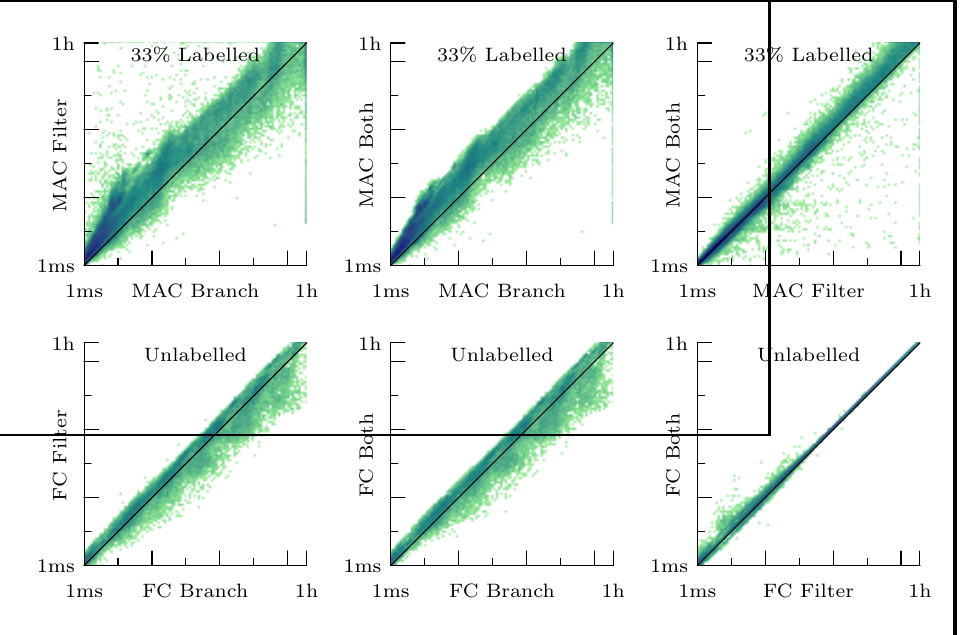
\begin{tikzpicture}[gnuplot]
%% generated with GNUPLOT 5.0p0 (Lua 5.2; terminal rev. 99, script rev. 100)
%% Wed 20 Apr 2016 12:04:43 AEST
\tikzset{every node/.append style={font={\scriptsize}}}
% \path (0.000,0.000) rectangle (11.684,7.620);
\gpcolor{color=gp lt color border}
\gpsetlinetype{gp lt border}
\gpsetdashtype{gp dt solid}
\gpsetlinewidth{1.00}
\draw[gp path] (0.442,7.251)--(0.442,4.426)--(3.268,4.426);
\node[gp node center,rotate=-270] at (0.140,5.838) {MAC Filter};
\node[gp node center] at (1.855,4.117) {MAC Branch};
\begin{scope}
\clip (0.442,7.251) rectangle (3.268,4.426);
\def\gprawrgbimagedata{%
  ffffffffffffffffffffffffffffffffffffffffffffffffffffff79d48d9cea9c85de9179d48d72cd8d85de919cea9c%
  85de919cea9c9cea9cffffff85de9185de9172cd8d85de9185de919cea9c72cd8d9cea9cffffffffffff85de91ffffff%
  72cd8d79d48d9cea9cffffff85de9185de91ffffff9cea9cffffff85de91ffffffffffff9cea9c85de9172cd8d79d48d%
  5eb98a9cea9c9cea9c72cd8d85de919cea9c85de916cc78c79d48d9cea9c9cea9c9cea9c85de9172cd8d9cea9c72cd8d%
  ffffff79d48d85de9185de9185de9185de919cea9c9cea9c9cea9cffffff79d48d9cea9c9cea9c9cea9c85de919cea9c%
  9cea9c79d48d9cea9c9cea9c6cc78c56b28956b289228b821f7d821e8282278f83208a8243a1862e9384339684339684%
  3195842c92831e8882268e83000080ffffffffffffffffffffffffffffffffffffffffffffffffffffffffffff9cea9c%
  ffffffffffffffffffffffffffffffffffffffffffffffffffffffffffffffffffffffffffffffffffffffffffffffff%
  ffffffffffffffffffffffffffffffffffffffffffffffffffffffffffffffffffffffffffffffffffffffffffffffff%
  ffffff9cea9c9cea9cffffffffffffffffffffffffffffffffffffffffffffffffffffffffffffffffffffffffffffff%
  ffffffffffffffffffffffffffffffffffffffffff9cea9cffffffffffffffffffffffffffffffffffffffffffffffff%
  ffffffffffffffffffffffffffffffffffffffffffffffff9cea9c6cc78c6cc78c48a586409f86409f8653af8850ac88%
  6cc78c72cd8d85de9179d48d79d48d72cd8d67c28b62bd8b5eb98a235e81ffffffffffffffffffffffffffffffffffff%
  ffffffffffffffffffffffffffffffffffffffffffffffffffffffffffffffffffffffffffffffffffffffffffffffff%
  ffffffffffffffffffffffffffffffffffffffffffffffffffffff9cea9cffffffffffffffffffffffffffffffffffff%
  ffffffffffffffffffffffffffffffffffffffffffffffffffffff9cea9cffffffffffffffffffffffff9cea9cffffff%
  ffffffffffffffffffffffffffffffffffffffffffffffffffffffffffffffffffffffffffffffffffffffffffffffff%
  ffffffffffffffffffffffffffffffffffffffffffffffffffffffffffffffffffffffffffffff72cd8d72cd8d6cc78c%
  56b2893396843e9d8545a2864da9875ab5895eb98a5ab58985de9162bd8bffffff67c28b6cc78c6cc78c235e81ffffff%
  ffffffffffffffffffffffffffffffffffffffffffffffffffffffffffffffffffffffffffffffffffffffffffffffff%
  9cea9cffffffffffffffffffffffffffffffffffffffffffffffffffffffffffffffffffffffffffffffffffffffffff%
  ffffffffffffffffffffffffffffffffffffffffffffffffffffffffffffffffffffffffffffff9cea9cffffffffffff%
  ffffffffffffffffffffffffffffffffffffffffff9cea9cffffffffffffffffffffffffffffffffffffffffffffffff%
  ffffffffffffffffffffffffffffffffffffffffffffffffffffffffffffffffffffffffffffffffffffffffff9cea9c%
  ffffff9cea9c72cd8d6cc78c4da98748a5862f94843b9c853b9c855eb98a72cd8d67c28b62bd8b5eb98a6cc78c5eb98a%
  62bd8b6cc78c72cd8d226181ffffffffffffffffffffffffffffffffffffffffffffffffffffffffffffffffffffffff%
  ffffffffffffffffffffffffffffffffffffffffffffffffffffffffffffffffffffffffffffffffffffffffffffffff%
  ffffffffffffffffffffffffffffffffffffffffffffffffffffffffffffffffffffffffffffffffffffffffffffffff%
  ffffffffffffffffffffffffffffffffffffffffffffffffffffffffffffffffffffffffffffffffffffffffffffffff%
  ffffffffffffffffffffffffffffffffffffffffffffffffffffffffffffffffffffffffffffffffffffffffffffffff%
  ffffffffffffffffffffffffffffff79d48d9cea9c62bd8b6cc78c56b289399a853e9d8545a28645a28645a28656b289%
  79d48d67c28b5ab58953af886cc78c6cc78c72cd8d5ab589226481ffffffffffffffffffffffffffffffffffffffffff%
  ffffffffffffffffffffffffffffffffffffffffffffffffffffffffffffffffffffffffffffffffffffffffffffffff%
  ffffffffffffffffffffffffffffffffffffffffffffffffffffffffffffffffffffffffffffffffffffffffffffffff%
  ffffffffffff9cea9cffffffffffffffffffffffffffffffffffffffffffffffffffffffffffffffffffffffffffffff%
  ffffffffffffffffffffffffffffffffffffffffffffffffffffffffffffffffffffffffffffffffffffffffffffffff%
  ffffffffffffffffff9cea9cffffffffffffffffffffffffffffffffffff79d48d72cd8d6cc78c45a2864aa78743a186%
  43a1862e938456b28972cd8d67c28b79d48d62bd8b62bd8b72cd8d79d48d5eb98a53af8862bd8b235f81ffffffffffff%
  ffffffffffffffffffffffffffffffffffffffffffffffffffffffffffffffffffffffffffffffffffffffffffffffff%
  ffffffffffffffffffffffffffffffffffffffffffffffffffffffffffffffffffffffffffffffffffffffffffffffff%
  ffffffffffffffffff9cea9cffffffffffffffffffffffffffffff9cea9cffffffffffffffffffffffffffffffffffff%
  ffffffffffffffffffffffffffffffffffff9cea9cffffffffffffffffffffffffffffffffffffffffffffffffffffff%
  ffffffffffffffffffffffffffffffffffffffffffffffffffffff9cea9cffffffffffff9cea9c9cea9cffffff85de91%
  62bd8b6cc78c409f864da98743a18645a2863b9c854da9874da9874da98767c28b53af885ab58972cd8d67c28b62bd8b%
  6cc78c53af88216581ffffffffffffffffffffffffffffffffffffffffffffffffffffffffffffffffffffffffffffff%
  ffffffffffffffffffffffffffffffffffffffffffffffffffffffffffffffffffffffffffffffffffffffffffffffff%
  ffffffffffffffffffffffffffffffffffffffffffffffffffffffffffffffffffffffffffffffffffffffffffffffff%
  ffffffffffffffffffffffff9cea9cffffffffffffffffffffffffffffffffffffffffffffffffffffffffffffffffff%
  ffffffffffffffffffffffffffffffffffffffffffffffff9cea9cffffffffffffffffffffffffffffff85de9185de91%
  85de91ffffff67c28b85de916cc78c6cc78c5eb98a45a2863e9d854da98735988445a28653af8853af886cc78c5ab589%
  62bd8b5eb98a5eb98a79d48d85de9172cd8d79d48d236081ffffffffffffffffffffffffffffffffffffffffffffffff%
  ffffffffffffffffffffffffffffffffffffffffffffffffffffffffffffffffffffffffffffffffffffffffffffffff%
  ffffffffffff9cea9cffffffffffffffffffffffffffffffffffffffffffffffffffffffffffffffffffffffffffffff%
  ffffffffffffffffff9cea9cffffffffffffffffffffffffffffffffffffffffffffffffffffffffffffffffffffffff%
  ffffffffffff9cea9cffffffffffffffffffffffffffffffffffff9cea9cffffffffffffffffffffffffffffffffffff%
  ffffffffffff9cea9c85de91ffffff9cea9c72cd8d9cea9c85de9179d48d6cc78c5eb98a409f864aa7873396843b9c85%
  2f94844da9876cc78c5eb98a6cc78c62bd8b72cd8d5ab58956b28979d48d85de914aa787206e81ffffffffffffffffff%
  ffffffffffffffffffffffffffffffffffffffffffffffffffffffffffffffffffffffffffffffffffffffffffffffff%
  ffffffffffffffffffffffffffffffffffffffffffffffffffffffffffffffffffffffffffffffffffffffffffffffff%
  ffffffffffffffffffffffffffffffffffffffffffffffffffffffffffffffffffffffffffffffffffffffffffffffff%
  ffffffffffffffffffffffffffffffffffffffffffffffffffffffffffffffffffffffff85de91ffffffffffffffffff%
  ffffffffffffffffffffffffffffffffffffffffff79d48d85de9172cd8d62bd8b79d48d67c28b85de915eb98a5eb98a%
  53af88399a8535988450ac883195844da98750ac8862bd8b72cd8d79d48d53af886cc78c62bd8b67c28b67c28b6cc78c%
  4aa787207181ffffffffffffffffffffffffffffffffffffffffffffffffffffffffffffffffffffffffffffffffffff%
  ffffffffffffffffffffffffffffffffffffffffffffffffffffffffffffffffffffffffffffffffffffffffffffffff%
  ffffffffffffffffffffffffffffffffffffffffffffffffffffffffffffffffffffffffffffffffffff9cea9cffffff%
  ffffffffffffffffffffffffffffffffffffffffffffffffffffffffffffffffffffffffffffffffffffffffffffffff%
  ffffffffffffffffffffffffffffffffffffffffffffffffffffffffffffffffffffffff79d48d79d48d67c28b62bd8b%
  79d48d5eb98a67c28b56b28956b28950ac8843a1863e9d8531958443a18648a58656b28956b28967c28b5eb98a6cc78c%
  62bd8b6cc78c67c28b67c28b6cc78c56b2891f7881ffffffffffffffffffffffffffffffffffffffffff9cea9cffffff%
  ffffffffffffffffffffffffffffffffffffffffff9cea9cffffffffffffffffffffffffffffff9cea9cffffffffffff%
  ffffffffffffffffff9cea9cffffffffffffffffffffffffffffffffffffffffffffffffffffffffffffffffff9cea9c%
  ffffffffffffffffffffffffffffffffffffffffffffffffffffffffffffffffffffffffffffff9cea9cffffffffffff%
  ffffffffffffffffffffffffffffffffffffffffffffffffffffffffffffffffffffffffffffffffffff9cea9cffffff%
  85de9172cd8d72cd8d5ab58953af8850ac8867c28b5ab5896cc78c53af8853af883195843b9c853396842f9484379985%
  56b28950ac8862bd8b5ab5895eb98a67c28b62bd8b79d48d50ac8872cd8d56b2891f7881ffffffffffffffffffffffff%
  ffffffffffffffffff9cea9cffffffffffffffffffffffffffffffffffffffffffffffffffffffffffffffffffffffff%
  ffffffffffffffffffffffffffffffffffffffffffffffffffffffffffffffffffffffffffffffffffffffffffffffff%
  ffffffffffffffffffffffffffffffffffffffffffffffffffffffffffffffffffffffffffffffffffffffffffffffff%
  ffffffffffffffffffffffffffffffffffffffffffffffffffffffffffffffffffffffffffffffffffffffffffffffff%
  ffffffffffff9cea9cffffff9cea9c79d48d72cd8d72cd8d53af8850ac8856b28956b2895ab58956b28953af8848a586%
  268e832e938433968429908345a2865ab58962bd8b79d48d6cc78c67c28b67c28b85de9179d48d9cea9c67c28b62bd8b%
  1f7881ffffffffffffffffffffffffffffffffffffffffff9cea9c9cea9cffffffffffffffffffffffffffffff9cea9c%
  ffffffffffffffffffffffffffffffffffffffffffffffffffffffffffffffffffffffffffffffffffffffffffffffff%
  ffffffffffffffffffffffffffffffffffffffffffffffffffffffffffffffffffffffffffffff9cea9cffffff9cea9c%
  9cea9cffffffffffffffffffffffffffffffffffffffffffffffffffffffffffffffffffffffffffffffffffffffffff%
  ffffffffffffffffffffffffffffffffffffffffff85de919cea9c85de916cc78c50ac8850ac8845a2863e9d854aa787%
  50ac8850ac8848a58656b28950ac88359884399a8535988431958453af885eb98a5eb98a67c28b67c28b67c28b67c28b%
  79d48d5ab58967c28b67c28b72cd8d1f8182ffffffffffffffffffffffffffffffffffffffffffffffffffffffffffff%
  ffffffffffffffffffffffff9cea9cffffffffffff9cea9cffffffffffffffffffffffffffffffffffffffffffffffff%
  ffffff9cea9cffffffffffffffffffffffffffffffffffffffffffffffffffffffffffffffffffffffffffffffffffff%
  ffffffffffffffffffffffffffffffffffffffffffffffffffffffffffffffffffffffffffffffffffffffffffffffff%
  ffffffffffffffffffffffffffffffffffffffffffffffffffffffffffffffffffffffffffffff79d48d85de915eb98a%
  56b28943a18648a58643a1863598844da98745a2864da9874da98743a18645a286409f8635988448a5865ab5894da987%
  5eb98a67c28b67c28b67c28b62bd8b67c28b79d48d85de9172cd8d67c28b208a82ffffffffffffffffffffffffffffff%
  ffffffffffffffffffffffffffffffffffffffffffffffffffffffffffffffffffffffffffffffffffffffffffffffff%
  ffffffffffffffffffffffffffffff9cea9cffffffffffffffffffffffffffffffffffff9cea9cffffffffffffffffff%
  ffffffffffffffffffffffffffffff9cea9cffffffffffffffffff9cea9cffffffffffffffffffffffffffffffffffff%
  ffffffffffffffffffffffffffffffffffffffffffffffffffffffffffffffffffffffffffffffffffffffffffffffff%
  85de919cea9c85de9167c28b4aa7873b9c8550ac883e9d8545a286339684399a8556b28962bd8b56b28950ac88238c83%
  409f863598842e938453af8862bd8b62bd8b79d48d79d48d6cc78c9cea9c85de9179d48d72cd8d72cd8d67c28b248d83%
  ffffffffffffffffffffffffffffffffffffffffffffffff9cea9cffffffffffffffffff9cea9cffffffffffffffffff%
  ffffffffffffffffffffffffffffffffffffffffffffffffffffffffffffffffffffffffffffff9cea9cffffff9cea9c%
  ffffffffffffffffffffffffffffffffffffffffff9cea9cffffffffffffffffffffffffffffffffffffffffffffffff%
  ffffffffffffffffffffffffffffffffffffffffffffffffffffffffffffffffff9cea9cffffffffffffffffffffffff%
  9cea9cffffffffffff9cea9c9cea9c85de91ffffff5eb98a4da9873598843e9d8548a58637998535988448a58643a186%
  50ac885eb98a56b2893799853799852c92834aa7875ab5895ab58967c28b9cea9c72cd8d72cd8d85de9167c28b85de91%
  79d48d72cd8d72cd8d67c28b359884ffffffffffffffffffffffffffffffffffffffffffffffffffffffffffffffffff%
  ffffffffffffffffffffffffffffffffffffffffffffffffffffffffffffffffffffffffffffffffffffffffffffffff%
  ffffffffffffffffffffffffffffffffffffffffffffffffffffff9cea9cffffffffffffffffffffffff9cea9cffffff%
  ffffff9cea9cffffffffffffffffffffffffffffffffffffffffffffffff9cea9cffffffffffff9cea9cffffffffffff%
  ffffffffffffffffffffffffffffffffffffffffffffffffffffff9cea9c9cea9c67c28b5eb98a4da987409f86248d83%
  248d833b9c853195843e9d85399a8553af8856b28948a5864aa7873b9c8548a58656b2894aa7876cc78c6cc78c5eb98a%
  67c28b62bd8b79d48d85de9185de9185de919cea9c79d48d85de91339684ffffffffffffffffffffffffffffffffffff%
  ffffffffffffffffffffffffffffffffffffffffffffffffffffffffffffffffff9cea9cffffffffffffffffffffffff%
  ffffffffffffffffffffffffffffffffffffffffffffffffffffffffffffffffffffffffffffffffffffffffffffffff%
  ffffffffffffffffffffffffffffffffffffffffffffffffffffffffffffffffffffffff9cea9cffffffffffffffffff%
  ffffffffffffffffffffffffffffffffffffffffffffffff9cea9cffffffffffffffffffffffff9cea9c85de915eb98a%
  4aa787409f86409f863598842f948431958437998545a28656b28962bd8b72cd8d5eb98a56b28948a58637998550ac88%
  62bd8b5ab5895eb98a79d48d6cc78c6cc78c85de9185de9172cd8d85de919cea9c72cd8d85de9172cd8d3b9c85ffffff%
  ffffffffffffffffffffffffffffffffffffffffffffffffffffffffffffffffffffffffffffffffffffffffffffffff%
  ffffffffffffffffffffffffffffffffffffffffffffffffffffffffffffffffffffffffffffff9cea9cffffffffffff%
  ffffffffffffffffffffffffffffffffffffffffffffffffffffffffffffffffff9cea9cffffffffffffffffffffffff%
  9cea9c9cea9cffffffffffffffffffffffffffffffffffffffffffffffffffffffffffffffffffffffffffffffffffff%
  85de9172cd8d85de9179d48d62bd8b48a586379985409f8643a186268e832990833e9d853e9d8550ac885ab58967c28b%
  79d48d56b28956b28953af8850ac884aa78762bd8b67c28b79d48d79d48d85de9185de9172cd8d72cd8d72cd8d72cd8d%
  85de9172cd8d79d48d379985ffffffffffffffffffffffffffffffffffffffffffffffffffffffffffffffffffffffff%
  9cea9cffffffffffffffffffffffffffffffffffffffffffffffffffffffffffffffffffffffffffffffffffffffffff%
  ffffffffffffffffffffffffffffffffffffffffffffffffffffffffffffffffffffffff9cea9cffffffffffffffffff%
  ffffffffffffffffffffffffffffffffffffffffffffffffffffffffffffffffffffffffffffffffffffffffff9cea9c%
  ffffffffffffffffffffffffffffffffffff62bd8b79d48d6cc78c3e9d8543a18645a2862f948448a5863598843e9d85%
  3e9d8545a28650ac8872cd8d67c28b67c28b50ac884da98737998545a28672cd8d67c28b6cc78c79d48d9cea9c6cc78c%
  79d48d85de9179d48d85de91ffffff67c28b85de919cea9c56b289ffffffffffffffffffffffffffffffffffffffffff%
  ffffffffffffffffffffffffffffffffffffffffffffffffffffffffffffffffffffffffffffffffffffffffffffffff%
  ffffffffffffffffffffffffffffffffffffffffffffffffffffffffffffffffffffffffffffffffffffffffffffffff%
  9cea9cffffffffffffffffffffffffffffffffffffffffffffffffffffffffffffffffff9cea9cffffffffffffffffff%
  ffffffffffffffffffffffffffffffffffff9cea9c85de919cea9c9cea9c85de915ab58953af88409f8650ac8845a286%
  37998548a58633968433968437998548a5864da98756b28962bd8b79d48d4da98762bd8b50ac8845a28662bd8b62bd8b%
  6cc78c6cc78c6cc78c72cd8d85de919cea9c79d48dffffff85de9172cd8d79d48d85de9185de914da987ffffffffffff%
  ffffffffffffffffffffffffffffffffffffffffffffffffffffffffffffffffffffffffffffff9cea9cffffffffffff%
  ffffff9cea9cffffffffffffffffffffffffffffffffffffffffffffffffffffff9cea9cffffffffffffffffffffffff%
  ffffffffffffffffffffffffffffffffffffffffffffffffffffffffffffffffffffffff9cea9cffffff9cea9cffffff%
  ffffffffffffffffffffffffffffffffffffffffffffffffffffffffffffffffff9cea9cffffffffffff79d48d6cc78c%
  43a18656b2893e9d853e9d854da9873598843799853b9c853396844aa78748a58650ac886cc78c6cc78c5ab5895eb98a%
  48a58653af8856b2895eb98a62bd8b72cd8d9cea9c6cc78c6cc78c9cea9c6cc78c9cea9cffffff85de919cea9c9cea9c%
  79d48d85de915eb98affffffffffffffffffffffffffffff9cea9cffffff9cea9cffffffffffffffffffffffffffffff%
  9cea9cffffffffffffffffffffffffffffffffffffffffffffffffffffffffffffffffffffffffffffffffffffffffff%
  ffffffffffffffffffffffffffffffffffffffffffffffffffffffffffffffffffffffffffffffffffffffffffffffff%
  ffffffffffff9cea9cffffffffffff9cea9cffffffffffffffffffffffff9cea9cffffffffffffffffffffffffffffff%
  ffffff79d48d9cea9c67c28b5ab58948a58633968445a2864da9873396843e9d8545a2863396844aa7873799854da987%
  53af8879d48d62bd8b53af8856b28943a1865ab58962bd8b62bd8b6cc78c62bd8b72cd8d9cea9c6cc78c9cea9c6cc78c%
  ffffffffffff9cea9cffffff9cea9cffffffffffff79d48dffffffffffffffffffffffffffffffffffffffffffffffff%
  9cea9cffffffffffffffffffffffffffffffffffffffffffffffffffffffffffffffffffffffffffffffffffffffffff%
  ffffffffffffffffffffffff9cea9cffffffffffffffffffffffffffffffffffffffffffffffffffffffffffff85de91%
  ffffffffffffffffff9cea9cffffffffffffffffffffffff85de91ffffffffffffffffffffffffffffffffffffffffff%
  ffffffffffffffffff9cea9c9cea9c85de9172cd8d6cc78c62bd8b45a28633968435988445a286339684399a85319584%
  3b9c85399a853799854da9875ab58953af886cc78c6cc78c53af884aa7874aa7876cc78c4aa78767c28b5eb98a72cd8d%
  9cea9c79d48d79d48dffffff72cd8d85de91ffffff79d48d79d48dffffff9cea9c9cea9c53af88ffffffffffffffffff%
  ffffffffffffffffffffffffffffffffffffffffffffffffffffffffffffffffffffffffffffffffffffffffffffffff%
  ffffffffffffffffffffffffffffffffffffffffffffffffffffffffffffffffffffffffffffffffffffffffffffffff%
  9cea9cffffffffffffffffff9cea9c9cea9cffffffffffffffffffffffff9cea9cffffffffffffffffffffffffffffff%
  ffffff9cea9cffffffffffff9cea9cffffffffffffffffffffffffffffff9cea9c62bd8b56b28967c28b409f86248d83%
  4aa78743a18650ac8835988445a2862e938435988453af88409f8656b28950ac8856b28953af8856b28950ac8862bd8b%
  62bd8b62bd8b72cd8d85de916cc78c79d48d9cea9c79d48d85de9185de919cea9cffffff85de91ffffff9cea9cffffff%
  ffffff67c28bffffffffffffffffffffffffffffffffffffffffffffffffffffffffffffffffffffffffffffffffffff%
  ffffffffffffffffffffffffffffffffffffffffffffffffffffffffffffffffffffffffffffffffffffffffffffffff%
  ffffffffffffffffffffffffffffff9cea9cffffffffffffffffff9cea9cffffffffffffffffffffffffffffffffffff%
  ffffff9cea9cffffffffffff9cea9c9cea9cffffffffffffffffff9cea9cffffffffffff79d48d9cea9c6cc78c6cc78c%
  5ab589399a8550ac88409f8629908345a286409f86409f8645a2864da987409f86409f8656b2894da9874da98762bd8b%
  4aa78748a58650ac885eb98a5ab58953af8862bd8b79d48d6cc78c72cd8d79d48d79d48d9cea9c85de919cea9c9cea9c%
  ffffffffffff9cea9cffffff9cea9cffffff72cd8dffffffffffffffffffffffffffffffffffffffffffffffffffffff%
  ffffffffffffffffffffffffffffffffffffffffffffffff9cea9cffffffffffffffffffffffffffffffffffffffffff%
  ffffffffffffffffffffffff9cea9cffffffffffffffffffffffffffffffffffffffffffffffffffffffffffffffffff%
  ffffff9cea9cffffffffffffffffff9cea9cffffff9cea9cffffffffffffffffffffffffffffffffffffffffff9cea9c%
  ffffff85de9172cd8d53af884aa787399a85399a8543a18645a286399a8550ac883b9c85339684409f8643a18645a286%
  4da98753af8850ac8867c28b5ab58985de915eb98a4aa78750ac885ab58979d48d50ac8872cd8d9cea9c79d48d85de91%
  9cea9c85de919cea9c9cea9c9cea9c85de91ffffffffffffffffffffffffffffff72cd8dffffffffffffffffffffffff%
  ffffffffffffffffffffffffffffffffffffffffffffffffffffffffffffffffffffffffffffffffffff9cea9cffffff%
  ffffffffffffffffffffffffffffffffffffffffffffffffffffffffffffffffff9cea9c9cea9cffffffffffffffffff%
  ffffffffffffffffffffffffffffffffffffffffffffffffffffffffffffffffffffffffffffff9cea9c9cea9cffffff%
  ffffff9cea9c9cea9cffffff85de919cea9c62bd8b5eb98a45a2863799853598843e9d853b9c8543a1862f9484409f86%
  48a58633968450ac8850ac8867c28b45a2865eb98a56b28967c28b67c28b5ab58972cd8d53af8856b28950ac88ffffff%
  6cc78c79d48d9cea9c85de919cea9c62bd8b85de91ffffffffffff85de919cea9cffffffffffffffffffffffffffffff%
  53af88ffffffffffffffffffffffffffffffffffffffffffffffffffffffffffffffffffffffffffffffffffffffffff%
  ffffffffffffffffffffffffffffffffffffffffffffffffffffffffffffffffffffffffffffffffffffffffffffffff%
  ffffffffffffffffffffffffffffff9cea9cffffffffffffffffffffffffffffffffffffffffffffffffffffff9cea9c%
  ffffffffffffffffff9cea9cffffffffffffffffff9cea9c9cea9c79d48d5ab58950ac8833968450ac8845a286399a85%
  409f8637998535988433968456b28943a1865eb98a4da98753af884aa7875eb98a5ab589409f8656b2895eb98a5ab589%
  50ac8879d48d4aa7875eb98a5ab5896cc78c79d48d85de9185de9179d48d9cea9c85de9185de91ffffff85de91ffffff%
  9cea9c9cea9c9cea9cffffffffffff5ab589ffffffffffffffffffffffffffffffffffff9cea9cffffffffffffffffff%
  ffffff9cea9cffffff9cea9cffffffffffffffffffffffffffffffffffffffffffffffffffffffffffffffffffffffff%
  ffffffffffffffffffffffffffffffffffffffffffffffffffffffffffffffffffffffffffffffffffffffffffffffff%
  ffffffffffffffffffffffffffffffffffffffffffffffffffffffffffffffffff85de919cea9c9cea9c62bd8b53af88%
  50ac8850ac883b9c852c92832f94843195843b9c8531958443a186399a855eb98a43a18662bd8b4da98756b28962bd8b%
  48a586409f866cc78c62bd8b5eb98a67c28b56b28967c28b5ab5896cc78c79d48d79d48dffffff9cea9c9cea9cffffff%
  85de91ffffffffffff9cea9cffffff9cea9c9cea9c9cea9cffffffffffff6cc78cffffffffffffffffffffffffffffff%
  ffffffffffffffffff9cea9cffffffffffff9cea9cffffffffffffffffffffffffffffffffffffffffffffffffffffff%
  ffffffffffffffffffffffffffffffffffffffffffffffffffffffffffffffffffffffff9cea9cffffffffffffffffff%
  ffffffffffffffffff9cea9cffffffffffffffffffffffffffffffffffff9cea9cffffffffffffffffff9cea9c9cea9c%
  9cea9c79d48d5eb98a3e9d8543a1864aa7873e9d85278f83409f862c928348a58643a1863b9c853598844da98756b289%
  50ac8850ac8848a5865ab5895eb98a45a28653af8862bd8b85de916cc78c5eb98a50ac8862bd8b72cd8d79d48d79d48d%
  9cea9cffffff9cea9c85de91ffffff9cea9cffffffffffffffffffffffffffffffffffffffffff9cea9cffffff53af88%
  ffffffffffffffffffffffffffffffffffffffffffffffffffffffffffffffffffffffffffffffffffffffffffffffff%
  ffffffffffffffffffffffffffffffffffffffffffffffffffffffffffff9cea9cffffffffffffffffffffffffffffff%
  ffffffffffff9cea9cffffffffffffffffffffffffffffffffffffffffffffffffffffffffffffffffff9cea9cffffff%
  85de91ffffffffffffffffffffffff9cea9c72cd8d409f8645a286399a8553af88268e83319584409f86409f8643a186%
  45a2863e9d8548a58656b2895ab58956b2895ab5895eb98a56b28962bd8b4da9874aa78750ac8856b28953af8867c28b%
  6cc78c72cd8d6cc78c85de919cea9c9cea9cffffff85de919cea9c9cea9c85de91ffffffffffff9cea9cffffff9cea9c%
  ffffff9cea9c85de91ffffff5ab589ffffffffffffffffffffffffffffffffffffffffffffffffffffffffffffffffff%
  9cea9c9cea9cffffffffffffffffff9cea9cffffffffffffffffffffffffffffffffffffffffffffffffffffffffffff%
  ffffffffffffffffffffffff9cea9cffffffffffffffffffffffffffffffffffffffffffffffffffffffffffffffffff%
  ffffffffffff85de91ffffffffffff9cea9c9cea9cffffff9cea9cffffff45a28648a58648a58643a1863b9c853e9d85%
  399a852f94843b9c85399a854da98767c28b3b9c8543a18653af885eb98a62bd8b4da9875ab5895ab58962bd8b5eb98a%
  56b28985de9179d48d72cd8d6cc78c6cc78c79d48d85de919cea9c85de919cea9cffffff85de9185de919cea9cffffff%
  ffffff9cea9c85de91ffffffffffff9cea9cffffffffffff9cea9c9cea9cffffffffffffffffffffffffffffffffffff%
  ffffffffffffffffffffffffffffffffffffffffffffffffffffffffffffffffffffffffffffffffffffffffffffffff%
  ffffffffffffffffffffffffffffffffffffffffffffffffffffffffffff9cea9cffffffffffffffffff9cea9cffffff%
  ffffffffffffffffffffffffffffffffffffffffffffffffffffff9cea9cffffff85de9185de919cea9c56b289409f86%
  3e9d85409f8648a58643a1865ab5894aa7873b9c8543a18643a18650ac8848a586409f864da98767c28b50ac883b9c85%
  5ab58962bd8b56b28950ac8856b2895eb98a72cd8d67c28b6cc78c79d48d56b28985de916cc78c85de9185de9185de91%
  ffffff72cd8dffffff85de9185de919cea9cffffffffffffffffff9cea9c85de91ffffffffffff9cea9c5eb98affffff%
  ffffffffffffffffffffffffffffffffffffffffffffffffffffffffffff9cea9cffffffffffffffffffffffffffffff%
  ffffffffffffffffffffffffffffffffffffffffffffffffffffffffffffffffffffffff9cea9cffffffffffffffffff%
  ffffff9cea9cffffffffffffffffffffffffffffffffffffffffffffffffffffff9cea9cffffffffffffffffffffffff%
  9cea9c5ab58962bd8b5eb98a3e9d85379985409f8643a1864da98745a2862e93843e9d8548a5863b9c85409f864aa787%
  56b2894da98772cd8d5eb98a67c28b5ab5895ab58967c28b62bd8b5ab58979d48d85de9185de916cc78c67c28b9cea9c%
  ffffff72cd8dffffff9cea9c9cea9c9cea9cffffff9cea9cffffff9cea9cffffffffffff9cea9cffffffffffffffffff%
  ffffffffffffffffff72cd8dffffffffffffffffffffffffffffffffffffffffffffffff9cea9cffffffffffffffffff%
  ffffff9cea9cffffffffffffffffffffffffffffffffffffffffffffffffffffffffffff9cea9cffffff9cea9cffffff%
  ffffffffffffffffffffffffffffffffffffffffffffffffffffffffffff9cea9cffffff9cea9cffffff9cea9c9cea9c%
  ffffff9cea9cffffff9cea9c9cea9c6cc78c6cc78c50ac8850ac88399a8545a2864da9874aa78743a186409f8656b289%
  409f8648a5865eb98a56b2894aa78753af886cc78c5eb98a67c28b45a28656b28979d48d79d48d53af8853af885ab589%
  85de9172cd8d72cd8d85de9179d48dffffff79d48d85de9185de919cea9cffffffffffff9cea9cffffff9cea9cffffff%
  ffffffffffff9cea9cffffffffffffffffffffffffffffff79d48dffffffffffffffffffffffffffffffffffffffffff%
  ffffffffffffffffffffffffffffffffffffffffffffffffffffffffffffffffffffffffffffff9cea9cffffffffffff%
  9cea9cffffffffffffffffffffffffffffffffffffffffffffffffffffffffffffffffff85de91ffffff9cea9cffffff%
  9cea9cffffffffffff85de91ffffff9cea9cffffff9cea9cffffff6cc78c67c28b3e9d8543a18643a1863b9c8545a286%
  4da98733968445a28653af884aa787409f8643a18662bd8b67c28b53af8853af8867c28b62bd8b53af8862bd8b5eb98a%
  5eb98a62bd8b5ab58979d48d85de9185de9179d48dffffff9cea9c79d48d9cea9cffffff85de91ffffff9cea9cffffff%
  ffffffffffff9cea9cffffffffffff9cea9cffffff9cea9cffffffffffffffffff85de91ffffff5ab589ffffffffffff%
  ffffffffffffffffffffffff9cea9cffffffffffffffffffffffffffffffffffffffffffffffffffffffffffffffffff%
  ffffffffffffffffffffffffffffffffffffffffffffffffffffffffffffffffffffffffffffffffffffffffffffffff%
  ffffffffffffffffffffffffffffff9cea9c85de91ffffff9cea9c9cea9c9cea9c79d48d6cc78c67c28b67c28b50ac88%
  399a854aa78743a1863b9c8550ac883e9d85409f865ab58945a2864da98750ac8850ac884da98762bd8b4da9875eb98a%
  5eb98a67c28b56b28956b2895eb98a72cd8d72cd8d85de9179d48dffffff9cea9c85de9172cd8dffffff79d48dffffff%
  9cea9c9cea9c6cc78c85de91ffffffffffff9cea9c9cea9c9cea9cffffffffffff9cea9cffffffffffffffffffffffff%
  ffffffffffff79d48dffffffffffffffffffffffffffffffffffffffffffffffffffffffffffffffffffffffffffffff%
  ffffffffffffffffffffffffffffffffffffffffffffffffffffffffffffffffffffffffffffffffffff9cea9c9cea9c%
  ffffffffffff9cea9cffffff9cea9cffffffffffffffffffffffffffffff85de91ffffff85de91ffffff85de919cea9c%
  ffffff72cd8d4da98756b2893195843396843598843e9d8543a18631958445a286409f865eb98a56b2893b9c855ab589%
  50ac8862bd8b6cc78c53af8867c28b5eb98a53af8856b28967c28b5eb98a85de9167c28b6cc78c85de9185de9172cd8d%
  9cea9c85de9185de9185de91ffffffffffffffffff9cea9c85de919cea9cffffff9cea9cffffffffffffffffffffffff%
  ffffffffffffffffffffffffffffffffffffffffff5ab589ffffffffffffffffffffffffffffffffffffffffffffffff%
  ffffffffffff9cea9cffffffffffffffffffffffffffffffffffff9cea9cffffffffffffffffffffffffffffffffffff%
  ffffff9cea9cffffffffffffffffffffffffffffffffffffffffffffffffffffffffffff9cea9c9cea9c85de9185de91%
  85de916cc78c85de9167c28bffffff9cea9c3b9c85399a8556b28943a186409f863b9c85409f864da9874da9874aa787%
  45a286399a8553af884da98753af886cc78c4da9875eb98a50ac8848a58662bd8b56b28956b2896cc78c85de916cc78c%
  79d48d6cc78c72cd8d9cea9cffffff85de919cea9cffffffffffff79d48d9cea9cffffffffffffffffffffffff9cea9c%
  ffffff9cea9cffffffffffffffffffffffff9cea9c9cea9cffffffffffffffffffffffff9cea9cffffffffffffffffff%
  9cea9cffffffffffffffffffffffffffffff9cea9cffffffffffff9cea9cffffff9cea9cffffffffffffffffffffffff%
  ffffffffffffffffffffffffffffffffffffffffffffffff9cea9cffffffffffffffffffffffffffffffffffff9cea9c%
  ffffffffffff9cea9c85de915eb98a62bd8b9cea9c9cea9c85de9172cd8d56b2893e9d854aa7873e9d853e9d8545a286%
  45a28650ac8850ac884da98745a28650ac8853af8848a5864da98743a18648a58653af8867c28b53af8867c28b6cc78c%
  67c28b56b2896cc78c79d48d67c28b9cea9cffffff72cd8d9cea9c9cea9c9cea9c9cea9c79d48d9cea9cffffffffffff%
  ffffffffffffffffffffffffffffff9cea9cffffffffffffffffffffffffffffffffffffffffffffffff9cea9cffffff%
  ffffff79d48dffffffffffffffffffffffffffffffffffffffffffffffffffffffffffffffffff9cea9cffffffffffff%
  9cea9cffffff9cea9c9cea9c9cea9cffffffffffffffffffffffffffffffffffffffffffffffffffffffffffffffffff%
  ffffffffffffffffffffffffffffffffffff9cea9c85de916cc78c5ab58948a5865ab58962bd8b62bd8b4da9874aa787%
  399a85359884409f864da9873598842f94843b9c8556b28950ac88409f86399a854aa78753af884da987409f8653af88%
  56b28967c28b5eb98a45a28667c28b79d48d6cc78c6cc78c85de919cea9c72cd8dffffff85de919cea9c9cea9c9cea9c%
  ffffffffffff9cea9c85de91ffffffffffffffffffffffffffffffffffffffffffffffffffffffffffffffffffffffff%
  ffffffffffffffffff9cea9cffffffffffff85de91ffffffffffffffffffffffffffffffffffffffffffffffffffffff%
  9cea9cffffffffffffffffffffffffffffffffffff9cea9cffffffffffff9cea9cffffffffffffffffffffffffffffff%
  ffffffffffffffffffffffffffffffffffffffffffffffffffffffffffffffffff79d48d6cc78c62bd8b4aa78745a286%
  4da9874aa78748a586359884379985299083399a855ab5893598843e9d852f948443a1865ab58950ac883e9d853b9c85%
  4da98756b28956b28967c28b48a58656b2895eb98a50ac885eb98a79d48d5eb98a6cc78c6cc78c85de9185de91ffffff%
  ffffff9cea9c79d48dffffff79d48d9cea9c9cea9cffffffffffffffffff79d48dffffffffffffffffffffffffffffff%
  ffffffffffffffffff9cea9cffffffffffffffffffffffffffffffffffffffffff79d48dffffffffffffffffffffffff%
  ffffffffffffffffffffffffffffffffffffffffffffffffffffffffffffffffffffffffffffff9cea9cffffffffffff%
  9cea9cffffffffffffffffffffffffffffffffffffffffffffffff9cea9cffffffffffffffffff9cea9c9cea9c9cea9c%
  85de9172cd8d50ac88399a8553af8843a1864aa7874aa7874da987399a852a918343a18650ac883b9c8548a58643a186%
  3e9d854aa7874aa7872990833e9d8556b28953af885ab5895eb98a56b2894da9874da987409f8653af8867c28b6cc78c%
  6cc78c72cd8d85de9185de9185de91ffffffffffffffffff9cea9cffffffffffff9cea9cffffffffffffffffffffffff%
  9cea9c9cea9cffffffffffffffffffffffffffffffffffffffffffffffffffffffffffffffffffffffffffffffffffff%
  67c28bffffffffffffffffffffffffffffffffffff9cea9cffffffffffff9cea9cffffffffffffffffffffffffffffff%
  ffffffffffffffffffffffffffffffffffffffffffffffffffffffffffffffffffffffffffffffffffffffffffffffff%
  ffffff9cea9cffffffffffff85de916cc78c56b28945a286268e8331958433968450ac8850ac8843a186359884339684%
  3195843e9d85399a8550ac8867c28b409f8650ac8856b289409f8650ac8850ac884aa78748a58653af8845a2863e9d85%
  5eb98a5eb98a53af886cc78c79d48d72cd8d62bd8b67c28b79d48dffffff85de91ffffff9cea9cffffff9cea9cffffff%
  ffffff9cea9cffffffffffffffffffffffffffffffffffffffffffffffffffffffffffffffffffffffffffffffffffff%
  ffffffffffffffffffffffffffffff85de91ffffffffffffffffffffffffffffffffffffffffffffffff9cea9cffffff%
  ffffffffffffffffffffffff9cea9c9cea9cffffffffffff9cea9cffffffffffffffffffffffffffffffffffffffffff%
  ffffffffffffffffffffffffffffffffffff9cea9cffffff9cea9c79d48d50ac883195843799851e87822c9283409f86%
  48a58643a1863396843799853396842e93843598843799853b9c853b9c8543a186409f86399a854aa7874da98753af88%
  4aa78737998550ac8856b28967c28b50ac8853af8872cd8d79d48d85de9179d48d9cea9c9cea9c72cd8d9cea9cffffff%
  ffffffffffffffffffffffffffffffffffff9cea9cffffff9cea9cffffff9cea9cffffffffffffffffffffffff9cea9c%
  ffffffffffffffffffffffffffffffffffffffffffffffffffffffffffff9cea9cffffffffffffffffffffffffffffff%
  ffffffffffffffffff79d48dffffffffffffffffff9cea9cffffff9cea9cffffff85de919cea9cffffff9cea9cffffff%
  ffffffffffffffffffffffffffffffffffff9cea9cffffffffffffffffffffffffffffffffffff85de9156b28950ac88%
  3396841e82821e87823195843598843396843e9d8537998545a286359884248d832c9283248d832f948450ac884da987%
  409f8648a58643a18645a28645a28656b28948a58662bd8b4aa78762bd8b43a1865eb98a72cd8d67c28b6cc78c85de91%
  9cea9c85de91ffffffffffff9cea9c9cea9c85de91ffffff9cea9cffffffffffffffffffffffff9cea9cffffffffffff%
  ffffffffffffffffffffffff9cea9cffffffffffffffffffffffffffffffffffffffffffffffffffffffffffff85de91%
  ffffffffffffffffffffffffffffffffffffffffffffffffffffffffffffffffffffffffffffffffffffffffff9cea9c%
  ffffffffffffffffffffffffffffffffffffffffffffffff9cea9cffffffffffffffffffffffffffffff85de91ffffff%
  79d48d85de9162bd8b53af881e89822c92831f7e82208a823598843195843598842990832e9384339684399a85268e83%
  228b823e9d8545a2863e9d853b9c8535988445a28643a1864aa7875eb98a5eb98a50ac885eb98a5eb98a4da98762bd8b%
  79d48d67c28b6cc78c62bd8b85de9185de91ffffff9cea9c79d48d9cea9c9cea9cffffff9cea9cffffffffffff9cea9c%
  ffffffffffffffffffffffffffffffffffffffffff9cea9cffffffffffffffffffffffffffffffffffffffffffffffff%
  ffffffffffffffffffffffff9cea9cffffffffffffffffffffffffffffffffffffffffffffffffffffffffffffffffff%
  9cea9cffffffffffffffffffffffffffffff9cea9cffffffffffffffffffffffffffffffffffffffffffffffffffffff%
  ffffffffffff6cc78c72cd8d62bd8b85de919cea9c67c28b45a2862a9183228b821e86822990831f8a82319584238c83%
  2e9384248d832f94842990831f8a821e8582228b82409f863b9c8543a18653af884aa78750ac884da98753af884aa787%
  5eb98a5eb98a6cc78c53af885ab58972cd8d67c28b79d48d9cea9c85de919cea9c9cea9c85de91ffffffffffff85de91%
  ffffffffffffffffffffffff9cea9c9cea9cffffffffffffffffffffffffffffffffffffffffffffffffffffffffffff%
  ffffffffffffffffffffffffffffffffffffffffffffffffffffff9cea9cffffffffffffffffffffffff9cea9cffffff%
  9cea9cffffff9cea9cffffffffffff9cea9cffffffffffffffffffffffff9cea9cffffffffffff9cea9cffffffffffff%
  9cea9cffffffffffffffffff9cea9c85de916cc78c2e93845ab58972cd8d9cea9c6cc78c67c28b43a1861e87821e8582%
  1e8282208a822c92833195842990832990833799853598842a91832c928337998543a18650ac882f948445a28645a286%
  50ac8856b28956b2896cc78c53af8862bd8b62bd8b50ac889cea9c5ab58985de9172cd8d85de91ffffffffffffffffff%
  85de9179d48dffffff85de91ffffffffffffffffffffffffffffffffffffffffffffffff9cea9cffffffffffffffffff%
  ffffffffffffffffffffffffffffffffffffffffffffffffffffffffffffffffffffffffffffffffffff85de91ffffff%
  ffffffffffffffffffffffffffffffffffffffffffffffff9cea9cffffff9cea9cffffffffffff9cea9c9cea9c9cea9c%
  85de91ffffffffffffffffffffffffffffff9cea9cffffffffffffffffff9cea9c72cd8d3e9d8579d48dffffff85de91%
  53af88409f86248d831e87821e86821e8582248d83248d832a91832990833195843195843598843195842e9384319584%
  3b9c8550ac8845a2864aa78750ac8856b28956b28948a58653af8862bd8b6cc78c50ac8867c28b6cc78c72cd8d67c28b%
  6cc78c79d48d85de919cea9c9cea9c9cea9cffffffffffff9cea9cffffffffffffffffffffffff9cea9cffffffffffff%
  ffffffffffffffffffffffffffffffffffffffffff9cea9cffffffffffffffffffffffffffffffffffffffffffffffff%
  ffffffffffffffffff9cea9cffffffffffffffffffffffffffffffffffffffffff9cea9c9cea9c9cea9cffffffffffff%
  9cea9c9cea9cffffffffffffffffff85de91ffffffffffffffffffffffffffffffffffffffffff9cea9cffffff85de91%
  5eb98a85de9185de9185de915eb98a5ab589399a85228b822a91831f79811e8782268e832e93843396843396843b9c85%
  2a9183319584359884409f8643a1863e9d853799855ab58956b28967c28b6cc78c5ab58953af8856b2895ab58979d48d%
  6cc78c62bd8b85de916cc78c72cd8d9cea9c85de919cea9c9cea9c9cea9c9cea9cffffffffffffffffffffffffffffff%
  ffffff9cea9cffffffffffffffffffffffffffffffffffff9cea9cffffffffffffffffffffffffffffffffffffffffff%
  ffffffffffffffffffffffffffffffffffffffffffffffff9cea9cffffffffffffffffffffffffffffffffffffffffff%
  ffffffffffffffffffffffffffffffffffffffffffffffff9cea9c85de919cea9c9cea9cffffffffffffffffffffffff%
  ffffffffffffffffffffffff72cd8d9cea9c9cea9c9cea9c79d48d5ab58948a586228b821e83821e88821f8182268e83%
  1f8a822a91833e9d85299083268e83409f862f948445a2864da98737998553af885eb98a72cd8d53af8867c28b5ab589%
  53af8853af8885de9167c28b72cd8d9cea9c85de919cea9c9cea9c85de919cea9c85de91ffffff9cea9cffffffffffff%
  9cea9cffffffffffff9cea9cffffffffffffffffffffffffffffffffffffffffffffffffffffffffffffffffffffffff%
  ffffffffffffffffffffffffffffffffffffffffffffffffffffffffffffffffffffffffffffff6cc78cffffffffffff%
  ffffffffffffffffffffffffffffff9cea9cffffffffffff85de91ffffffffffffffffffffffff9cea9cffffffffffff%
  9cea9cffffffffffffffffffffffffffffffffffff85de919cea9cffffffffffff85de91ffffff4da987379985278f83%
  1f8a821e83821f81821f7b821e8282278f832c92832a9183208a822c928345a286409f86399a8545a2863b9c855eb98a%
  5eb98a5ab58972cd8d67c28b79d48d67c28b6cc78c85de9179d48d79d48d72cd8d9cea9c85de9179d48d9cea9c9cea9c%
  9cea9c85de91ffffffffffffffffff9cea9cffffffffffffffffffffffffffffffffffffffffffffffffffffffffffff%
  ffffffffffffffffffffffffffffffffffffffffffffffffffffffffffffffffffffffffffffffffffffffffffffffff%
  ffffffffffff67c28bffffffffffffffffff9cea9c9cea9cffffffffffffffffffffffffffffff9cea9c9cea9cffffff%
  ffffffffffffffffff85de91ffffffffffffffffff9cea9c85de919cea9cffffff79d48d67c28b72cd8dffffff9cea9c%
  5ab58967c28b409f864aa787228b821f8082206d811f76811f78811f80821e87822e93842e9384278f8343a1864aa787%
  3b9c8548a5865eb98a4aa78753af885eb98a5eb98a72cd8d5ab58972cd8d85de9162bd8b79d48d72cd8d85de919cea9c%
  6cc78c72cd8dffffffffffff9cea9c9cea9c9cea9c9cea9cffffffffffffffffffffffffffffffffffffffffffffffff%
  ffffffffffffffffffffffffffffffffffffffffffffffffffffffffffffffffffffffffffffffffffffffffffffffff%
  ffffffffffffffffffffffffffffffffffffffffff79d48dffffffffffffffffffffffffffffff9cea9cffffffffffff%
  ffffffffffff9cea9cffffffffffff9cea9cffffffffffff72cd8dffffff9cea9cffffffffffff9cea9cffffff9cea9c%
  6cc78c5eb98a85de9179d48d67c28b4da9875ab58950ac883799852c92831f7f821f7e821f7c821f7b821e87821f8a82%
  2c92833e9d85409f8643a186409f8662bd8b62bd8b53af8856b2895eb98a67c28b5eb98a5ab58967c28b62bd8b85de91%
  85de9185de9185de91ffffff79d48dffffff85de919cea9cffffffffffffffffff9cea9c9cea9cffffffffffffffffff%
  ffffffffffffffffffffffffffffffffffffffffffffffffffffffffffffffffffffffffffffffffffffffffffffffff%
  ffffffffffffffffffffffffffffffffffffffffffffffffffffffffffffffffffffffff85de91ffffffffffffffffff%
  ffffffffffffffffffffffffffffff9cea9c85de91ffffffffffffffffff9cea9c85de91ffffff85de91ffffff79d48d%
  85de915eb98a9cea9c85de9156b289399a8585de919cea9c6cc78c5eb98a5ab5893b9c854da9872a9183228b821f7481%
  206e811f74811e8782278f832c928345a28643a1863b9c8556b28967c28b5ab5895eb98a67c28b67c28b79d48d85de91%
  79d48d4aa7879cea9c72cd8d67c28b79d48d72cd8d85de9185de91ffffff85de9179d48dffffffffffffffffff85de91%
  9cea9cffffffffffffffffffffffffffffffffffffffffffffffffffffffffffffffffffffffffffffffffffffffffff%
  ffffffffffffffffffffffffffffffffffffffffffffffffffffffffffffffffffffffffffffffffffffffffffffffff%
  ffffff79d48dffffffffffffffffffffffff9cea9cffffff9cea9cffffff9cea9cffffff9cea9cffffff9cea9cffffff%
  ffffff9cea9cffffffffffff6cc78c5ab58972cd8d72cd8d85de91409f8667c28b79d48d79d48d67c28b5ab5894aa787%
  4aa7872e93841f7b821f7e821f7c821f76811f7b821e86822990834aa78743a1864da9875ab58950ac885ab5894da987%
  67c28b62bd8b67c28b72cd8d62bd8b56b28962bd8b85de9185de9185de9167c28b85de9185de919cea9c9cea9c9cea9c%
  9cea9cffffff85de91ffffffffffffffffffffffffffffffffffffffffffffffffffffffffffffffffffffffffffffff%
  ffffffffffffffffffffffffffffffffffffffffffffffffffffffffffffffffffffffffffffffffffffffffffffffff%
  ffffffffffffffffffffffffffffffffffff85de91ffffffffffffffffff9cea9c9cea9c9cea9cffffff85de91ffffff%
  ffffff9cea9c9cea9cffffffffffffffffff85de9167c28bffffff48a586409f8650ac8885de9162bd8b5eb98a9cea9c%
  79d48d67c28b409f8643a186339684278f831e87821f79811f7f821f7e821f74811e8282238c834aa787409f8650ac88%
  4da98762bd8b5eb98a62bd8b79d48d67c28b72cd8d6cc78c85de9185de9162bd8b79d48d85de9179d48d79d48dffffff%
  9cea9c9cea9cffffff9cea9c9cea9cffffffffffffffffff9cea9c9cea9cffffffffffffffffffffffffffffffffffff%
  ffffffffffff9cea9cffffffffffffffffffffffffffffffffffffffffffffffffffffffffffffffffffffffffffffff%
  ffffffffffffffffffffffffffffffffffffffffffffffffffffffffffffffffff85de91ffffffffffffffffffffffff%
  ffffffffffff9cea9cffffffffffff9cea9c9cea9cffffff9cea9c9cea9c85de91ffffff72cd8d79d48d3e9d853e9d85%
  5eb98a67c28b67c28b9cea9c56b28956b2894aa7873e9d85409f863e9d852990831f7f821f80821f74811f7d821f7e82%
  208a8233968435988445a28650ac886cc78c85de9150ac8867c28b72cd8d6cc78c72cd8d85de916cc78c6cc78c79d48d%
  9cea9c85de9185de9172cd8dffffffffffffffffff9cea9cffffffffffffffffffffffffffffffffffffffffffffffff%
  ffffffffffffffffffffffffffffffffffffffffffffffffffffffffffffffffffffffffffffffffffffffffffffffff%
  ffffffffffffffffffffffffffffffffffffffffffffffffffffffffffffffffffffffffffffffffffffffffffffffff%
  79d48dffffffffffffffffffffffff9cea9cffffff9cea9cffffffffffff85de91ffffffffffff9cea9cffffff85de91%
  72cd8d72cd8d62bd8b3e9d8543a18667c28b62bd8b62bd8b5eb98a62bd8b399a8543a18643a1863b9c85379985238c83%
  1e89821f7d821e85821e88821f7f82228b8243a186409f8650ac8872cd8d62bd8b5eb98a72cd8d79d48d85de919cea9c%
  9cea9c6cc78c79d48d9cea9c85de9172cd8dffffff9cea9c9cea9c85de91ffffff9cea9cffffff85de919cea9cffffff%
  ffffffffffffffffffffffffffffffffffffffffffffffffffffffffffffffffffffffffffffffffffffffffffffffff%
  ffffffffffffffffffffffffffffffffffffffffffffffffffffffffffffffffffffffffffffffffffffffffffffffff%
  ffffffffffffffffffffffffffffff79d48dffffffffffffffffff9cea9c9cea9cffffff9cea9cffffff9cea9cffffff%
  9cea9c9cea9cffffff9cea9cffffff85de916cc78c79d48d268e833598845ab5894aa7875ab5894da987359884379985%
  45a2863b9c85228b821e8582228b821e83821e82821e88821f8a821e8782228b823b9c854da98772cd8d6cc78c67c28b%
  79d48d79d48d85de9179d48d9cea9c85de919cea9c85de9172cd8d9cea9c9cea9c9cea9c85de91ffffffffffff9cea9c%
  ffffff9cea9cffffffffffffffffffffffff9cea9cffffffffffffffffffffffffffffffffffffffffffffffffffffff%
  ffffffffffffffffffffffffffffffffffffffffffffffffffffffffffffffffffffffffffffffffffffffffffffffff%
  ffffffffffffffffffffffffffffffffffffffffffffffffffffffffffff79d48dffffffffffffffffffffffffffffff%
  ffffffffffffffffff85de91ffffff79d48d9cea9c9cea9c85de916cc78c6cc78c3b9c854da9872a91833799854aa787%
  53af8872cd8d56b2893799853396843799853396841f8a821f7d82208a821e8682248d831e89821f8a821f8a82339684%
  4da9874aa7876cc78c5ab5896cc78c85de919cea9c72cd8d72cd8dffffff6cc78c9cea9cffffffffffffffffffffffff%
  ffffffffffff9cea9c9cea9cffffffffffffffffffffffffffffffffffffffffffffffffffffff9cea9cffffffffffff%
  ffffffffffffffffffffffffffffffffffffffffffffffffffffffffffffffffffffffffffffffffffffffffffffffff%
  ffffffffffffffffffffffffffffffffffffffffffffffffffffffffffffffffffffffffffffffffffffffffff6cc78c%
  ffffffffffffffffffffffffffffffffffffffffffffffffffffff6cc78cffffff9cea9c9cea9c6cc78c79d48d43a186%
  4aa78748a586278f83319584409f865ab58972cd8d48a58631958433968443a186248d832990831e83821e8882208a82%
  1e87821e8582228b82278f83359884399a8556b28972cd8d5ab58985de9172cd8d85de919cea9cffffff9cea9cffffff%
  ffffff9cea9c9cea9cffffff85de919cea9c85de919cea9cffffffffffffffffffffffffffffffffffffffffffffffff%
  ffffffffffffffffffffffffffffffffffffffffffffffffffffffffffffffffffffffffffffffffffffffffffffffff%
  ffffffffffffffffffffffffffffffffffffffffffffffffffffffffffffffffffffffffffffffffffffffffffffffff%
  ffffffffffffffffffffffff72cd8dffffffffffffffffffffffffffffffffffffffffffffffffffffff9cea9cffffff%
  85de91ffffff72cd8d4da9873b9c8550ac88399a85248d834aa7875eb98a5eb98a3e9d851e87821e86823396842c9283%
  278f832e93841f7b82248d83299083248d83208a822c92831e89823e9d8556b28967c28b5eb98a85de9185de9179d48d%
  85de9185de9185de919cea9c85de9179d48d9cea9c9cea9c9cea9cffffff9cea9cffffffffffffffffffffffffffffff%
  9cea9cffffffffffffffffffffffffffffffffffffffffffffffffffffffffffffffffffffffffffffffffffffffffff%
  ffffffffffffffffffffffffffffffffffffffffffffffffffffffffffffffffffffffffffffffffffffffffffffffff%
  ffffffffffffffffffffffffffffffffffffffffffffffffffffff79d48dffffffffffffffffffffffffffffffffffff%
  ffffffffffffffffffffffff85de91ffffff9cea9c67c28b3b9c852e9384399a853b9c853195843e9d8562bd8b53af88%
  2c9283278f83238c83268e83278f83299083208a82208a82339684379985208a822e93842f94843e9d855ab58962bd8b%
  85de9185de91ffffff9cea9cffffff85de919cea9c9cea9cffffffffffff9cea9c9cea9cffffffffffff9cea9c85de91%
  9cea9cffffffffffffffffffffffffffffffffffffffffffffffffffffffffffffffffffffffffffffffffffffffffff%
  ffffffffffffffffffffffffffffffffffffffffffffffffffffffffffffffffffffffffffffffffffffffffffffffff%
  ffffffffffffffffffffffffffffffffffffffffffffffffffffffffffffffffffffffffffffffffffff72cd8dffffff%
  ffffffffffffffffffffffffffffff9cea9c79d48d9cea9c9cea9c79d48d85de919cea9c2f94842a9183208a822c9283%
  2e93842a91832e93844da9873b9c85238c831e8882248d831e89821e88822f94841f8a82278f83238c83379985228b82%
  4aa7873e9d854da9876cc78c79d48d6cc78c79d48d6cc78c9cea9cffffff9cea9c9cea9cffffff85de91ffffffffffff%
  ffffffffffffffffff9cea9cffffffffffffffffffffffffffffffffffffffffffffffffffffffffffffffffffffffff%
  ffffffffffffffffffffffffffffffffffffffffffffffffffffffffffffffffffffffffffffffffffffffffffffffff%
  ffffffffffffffffffffffffffffffffffffffffffffffffffffffffffffffffffffffffffffffffffffffffffffffff%
  ffffffffffffffffff79d48dffffffffffffffffffffffff9cea9cffffffffffffffffff9cea9cffffff85de91ffffff%
  67c28b339684268e831e89821f7f821f7f821f7c82268e83399a85228b82228b821e8882268e831e8382238c83208a82%
  238c832f94843b9c85319584238c8333968443a186399a855eb98a79d48d85de91ffffffffffff9cea9c9cea9c9cea9c%
  ffffffffffffffffffffffffffffffffffffffffffffffffffffffffffff9cea9cffffffffffffffffffffffffffffff%
  ffffffffffffffffffffffffffffffffffffffffffffffffffffffffffffffffffffffffffffffffffffffffffffffff%
  ffffffffffffffffffffffffffffffffffffffffffffffffffffffffffffffffffffffffffffffffffffffffffffffff%
  ffffffffffffffffffffffffffffffffffffffffffffffff72cd8dffffffffffffffffffffffffffffff9cea9cffffff%
  ffffffffffff67c28b9cea9c79d48d56b2891f76811f76811f81821f72812070811f7281299083319584278f831e8382%
  1f81821e85821f7e822f94842a9183238c833799854da987399a852f94842e93843e9d855ab5895eb98a79d48d9cea9c%
  79d48d9cea9c79d48d85de91ffffff9cea9cffffff9cea9cffffffffffffffffffffffff9cea9cffffffffffffffffff%
  ffffffffffffffffffffffffffffffffffffffffffffffffffffffffffffffffffffffffffffffffffffffffffffffff%
  ffffffffffffffffffffffffffffffffffffffffffffffffffffffffffffffffffffffffffffffffffffffffffffffff%
  ffffffffffffffffffffffffffffffffffffffffffffffffffffffffffffffffffffffffffffff6cc78cffffff9cea9c%
  ffffff9cea9cffffff9cea9c9cea9c9cea9c85de9172cd8d79d48d85de91339684206d81206d811f7781226181226181%
  1f7a822f9484228b821f80821f7f821f78811e82821e86822f9484238c83339684268e83409f86399a853195844aa787%
  409f8648a5865eb98a9cea9c85de9172cd8dffffff9cea9cffffffffffffffffffffffffffffffffffffffffffffffff%
  ffffffffffffffffffffffffffffffffffffffffffffffffffffffffffffffffffffffffffffffffffffffffffffffff%
  ffffffffffffffffff9cea9cffffffffffffffffffffffffffffffffffffffffffffffffffffffffffffffffffffffff%
  ffffffffffffffffffffffffffffffffffffffffffffffffffffffffffffffffffffffffffffffffffffffffffffffff%
  ffffffffffff79d48dffffffffffffffffffffffffffffffffffffffffff9cea9cffffff85de9167c28b6cc78c299083%
  235d81206981206b81265281265381238c83268e831f7e821f80821f72811f7f821e8682278f832c928337998543a186%
  278f833b9c85409f863e9d854aa78756b2895ab58979d48d79d48d85de91ffffff9cea9c9cea9cffffffffffffffffff%
  ffffffffffffffffffffffffffffffffffffffffffffffffffffff9cea9cffffffffffffffffffffffffffffffffffff%
  ffffffffffffffffffffffffffffffffffffffffffffffffffffffffffffffffffffffffffffffffffffffffffffffff%
  ffffffffffffffffffffffffffffffffffffffffffffffffffffffffffffffffffffffffffffffffffffffffffffffff%
  ffffffffffffffffffffffffffffffffffffffffff79d48dffffffffffff9cea9cffffff85de919cea9c85de919cea9c%
  85de9185de9172cd8d79d48d1f7481255881245b81235d812849812167811e87821e87821e89821e82821f74811f8182%
  2c92831f8a823e9d852f948437998533968443a1862f948443a1864aa78750ac886cc78c79d48d9cea9c79d48dffffff%
  ffffffffffffffffffffffffffffffffffffffffffffffffffffffffffffffffffffffffffffffffffffffffffffffff%
  ffffffffffffffffffffffffffffffffffffffffffffffffffffffffffffffffffffffffffffffffffffffffffffffff%
  ffffffffffffffffffffffffffffffffffffffffffffffffffffffffffffffffffffffffffffffffffffffffffffffff%
  ffffffffffffffffffffffffffffffffffffffffffffffffffffffffffffffffffffffff6cc78cffffffffffffffffff%
  9cea9cffffff85de91ffffff9cea9c79d48d79d48d62bd8b6cc78c206c81255881284c81265481226481228b82208a82%
  1e86821f7c821f7c821f7a821e8582268e83268e8329908345a2862a9183399a8543a18633968456b2894aa78762bd8b%
  5ab58972cd8d72cd8d9cea9cffffffffffffffffffffffffffffffffffffffffffffffffffffffffffffffffffffffff%
  ffffffffffffffffffffffffffffffffffffffffffffffffffffffffffffffffffffffffffffffffffffffffffffffff%
  ffffffffffffffffffffffffffffffffffffffffffffffffffffffffffffffffffffffffffffffffffffffffffffffff%
  ffffffffffffffffffffffffffffffffffffffffffffffffffffffffffffffffffffffffffffffffffffffffffffffff%
  ffffff6cc78cffffffffffffffffff9cea9cffffffffffff9cea9cffffff72cd8d79d48d56b2893e9d85206e81255581%
  274581235e811e8582248d831e86821f74811f75811f7c821f7c821e89822f9484228b82319584409f8633968448a586%
  43a1864aa7874aa78753af8853af8872cd8d72cd8d9cea9c9cea9cffffff9cea9cffffffffffffffffffffffffffffff%
  ffffffffffffffffffffffffffffffffffffffffffffffffffffffffffffffffffffffffffffffffffffffffffffffff%
  ffffffffffffffffffffffffffffffffffffffffffffffffffffffffffffffffffffffffffffffffffffffffffffffff%
  ffffffffffffffffffffffffffffffffffffffffffffffffffffffffffffffffffffffffffffffffffffffffffffffff%
  ffffffffffffffffffffffffffffffffffff67c28bffffffffffffffffffffffffffffff9cea9cffffff85de919cea9c%
  5ab58948a586299083235f812556812654811f7881238c831e86821f79811f73811f7c821e8282208a822990832f9484%
  43a1863598842a918345a2865ab5894da98748a5865ab58979d48d72cd8d72cd8d9cea9c9cea9c9cea9cffffff9cea9c%
  ffffffffffffffffffffffffffffffffffffffffffffffffffffffffffffffffffffffffffffffffffffffffffffffff%
  ffffffffffffffffffffffffffffffffffffffffffffffffffffffffffffffffffffffffffffffffffffffffffffffff%
  ffffffffffffffffffffffffffffffffffffffffffffffffffffffffffffffffffffffffffffffffffffffffffffffff%
  ffffffffffffffffffffffffffffffffffffffffffffffffffffffffffffffffff72cd8d9cea9c85de91ffffffffffff%
  ffffff9cea9c9cea9c9cea9c85de9150ac883598841e8282255981235d81206f811e83821f7b821f7b821f7c821f7881%
  1e87821e88822990832f94844da987399a8545a28645a28643a18653af884aa78767c28b79d48d67c28b85de9179d48d%
  ffffff9cea9c9cea9cffffffffffffffffffffffffffffffffffffffffffffffffffffffffffffffffffffffffffffff%
  ffffffffffffffffffffffffffffffffffffffffffffffffffffffffffffffffffffffffffffffffffffffffffffffff%
  ffffffffffffffffffffffffffffffffffffffffffffffffffffffffffffffffffffffffffffffffffffffffffffffff%
  ffffffffffffffffffffffffffffffffffffffffffffffffffffffffffffffffffffffffffffffffffffffffffffffff%
  62bd8bffffffffffffffffffffffff9cea9cffffffffffff85de9179d48d43a1861f8082206f812654812070811f7881%
  1f7a821f7f822071811f76811f7d821e84822a918335988453af883e9d854aa78743a18643a18653af8856b28979d48d%
  62bd8b53af8879d48d9cea9c9cea9c85de919cea9c9cea9cffffffffffffffffffffffffffffffffffffffffffffffff%
  ffffffffffffffffffffffffffffffffffffffffffffffffffffffffffffffffffffffffffffffffffffffffffffffff%
  ffffffffffffffffffffffffffffffffffffffffffffffffffffffffffffffffffffffffffffffffffffffffffffffff%
  ffffffffffffffffffffffffffffffffffffffffffffffffffffffffffffffffffffffffffffffffffffffffffffffff%
  ffffffffffffffffffffffffffffff67c28bffffffffffffffffff9cea9c9cea9c85de9179d48d67c28b5eb98a228b82%
  206d812557812167811f76811f7681206e81206f811f7a821f79811f7f82208a822e938435988456b2893b9c85359884%
  48a58653af8856b2895eb98a5ab58967c28b9cea9c79d48d79d48d9cea9cffffff9cea9cffffffffffffffffffffffff%
  ffffffffffffffffffffffffffffffffffffffffffffffffffffffffffffffffffffffffffffffffffffffffffffffff%
  ffffffffffffffffffffffffffffffffffffffffffffffffffffffffffffffffffffffffffffffffffffffffffffffff%
  ffffffffffffffffffffffffffffffffffffffffffffffffffffffffffffffffffffffffffffffffffffffffffffffff%
  ffffffffffffffffffffffffffffffffffffffffffffffffffffffffffff67c28b9cea9cffffffffffff79d48dffffff%
  9cea9c85de916cc78c50ac881f7881255881255581207181207181216681235f811f72811f7e821f7c821e8882248d83%
  3b9c852e9384399a8553af885eb98a53af8856b2895ab5896cc78c62bd8b85de9179d48d85de91ffffffffffffffffff%
  ffffffffffffffffffffffffffffffffffffffffffffffffffffffffffffffffffffffffffffffffffffffffffffffff%
  ffffffffffffffffffffffffffffffffffffffffffffffffffffffffffffffffffffffffffffffffffffffffffffffff%
  ffffffffffffffffffffffffffffffffffffffffffffffffffffffffffffffffffffffffffffffffffffffffffffffff%
  ffffffffffffffffffffffffffffffffffffffffffffffffffffffffffffffffffffffffffffffffffffffffff5eb98a%
  ffffffffffffffffff9cea9cffffff9cea9c79d48d53af883e9d85216781255681245c81206c81216781216681216881%
  1f74811f7c821e88822c92832a918348a5864aa78762bd8b4da98743a1865ab58956b2896cc78c72cd8dffffff79d48d%
  9cea9c85de9185de91ffffffffffff9cea9cffffffffffffffffffffffffffffffffffffffffffffffffffffffffffff%
  ffffffffffffffffffffffffffffffffffffffffffffffffffffffffffffffffffffffffffffffffffffffffffffffff%
  ffffffffffffffffffffffffffffffffffffffffffffffffffffffffffffffffffffffffffffffffffffffffffffffff%
  ffffffffffffffffffffffffffffffffffffffffffffffffffffffffffffffffffffffffffffffffffffffffffffffff%
  ffffffffffffffffffffffff50ac88ffffffffffff85de919cea9c9cea9c72cd8d79d48d43a1861f7881245a81255781%
  245b81235e812360812360812168812070811f7f821f7f82248d832f948456b28950ac885eb98a50ac8848a58672cd8d%
  67c28b6cc78cffffff6cc78c85de919cea9cffffffffffff9cea9cffffffffffffffffffffffffffffffffffffffffff%
  ffffffffffffffffffffffffffffffffffffffffffffffffffffffffffffffffffffffffffffffffffffffffffffffff%
  ffffffffffffffffffffffffffffffffffffffffffffffffffffffffffffffffffffffffffffffffffffffffffffffff%
  ffffffffffffffffffffffffffffffffffffffffffffffffffffffffffffffffffffffffffffffffffffffffffffffff%
  ffffffffffffffffffffffffffffffffffffffffffffffffffffff62bd8bffffffffffff85de919cea9c79d48d72cd8d%
  50ac881e8282206981274f81284c81255881235d812261812263812168811f75811f8182268e83208a824da98750ac88%
  50ac8850ac8862bd8b67c28b79d48d6cc78c67c28b85de919cea9c85de91ffffffffffffffffffffffffffffffffffff%
  9cea9cffffffffffffffffffffffffffffffffffffffffffffffffffffffffffffffffffffffffffffffffffffffffff%
  ffffffffffffffffffffffffffffffffffffffffffffffffffffffffffffffffffffffffffffffffffffffffffffffff%
  ffffffffffffffffffffffffffffffffffffffffffffffffffffffffffffffffffffffffffffffffffffffffffffffff%
  9cea9cffffffffffffffffffffffffffffffffffffffffffffffffffffffffffffffffffffffffffffffffffffffffff%
  ffffffffffff9cea9c85de9172cd8d45a286206d81275081284981255581265481255681226181206b81206d811f7f82%
  2f948431958445a28645a2866cc78c56b28950ac8856b2896cc78c85de91ffffffffffff79d48dffffffffffffffffff%
  ffffffffffffffffffffffffffffffffffffffffffffffffffffffffffffffffffffffffffffffffffffffffffffffff%
  ffffffffffffffffffffffffffffffffffffffffffffffffffffffffffffffffffffffffffffffffffffffffffffffff%
  ffffffffffffffffffffffffffffffffffffffffffffffffffffffffffffffffffffffffffffffffffffffffffffffff%
  ffffffffffffffffffffffffffffffffffffffffffffffffffffffffffffffffffffffffffffffffffffffffffffffff%
  ffffffffffffffffffffffff79d48d85de919cea9c85de9185de9185de91268e83265481275081265381274f81265281%
  235f812166812262811f7b821e86821e88823396845ab58948a58667c28b85de9162bd8b85de9172cd8d79d48d79d48d%
  ffffffffffff9cea9cffffffffffff9cea9cffffffffffffffffffffffffffffffffffffffffffffffffffffffffffff%
  ffffffffffffffffffffffffffffffffffffffffffffffffffffffffffffffffffffffffffffffffffffffffffffffff%
  ffffffffffffffffffffffffffffffffffffffffffffffffffffffffffffffffffffffffffffffffffffffffffffffff%
  ffffffffffffffffffffffffffffffffffffffffffffffffffffffffffffffffffffffffffffffffffffffffffffffff%
  ffffffffffffffffffffffffffffffffffffffffffffffffffffffffffffffffffffffff6cc78c79d48d45a2861f7281%
  265481255781274881274f812559812556812264811f79811f7e82278f8329908345a2865ab58972cd8d9cea9c85de91%
  72cd8d6cc78c79d48d85de91ffffff9cea9cffffffffffffffffff9cea9cffffffffffffffffffffffffffffffffffff%
  ffffffffffffffffffffffffffffffffffffffffffffffffffffffffffffffffffffffffffffffffffffffffffffffff%
  ffffffffffffffffffffffffffffffffffffffffffffffffffffffffffffffffffffffffffffffffffffffffffffffff%
  ffffffffffffffffffffffffffffffffffffffffffffffffffffffffffffffffffffffffffffffffffffffffffffffff%
  ffffffffffffffffffffffffffffffffffffffffffffffffffffffffffffffffffffffffffffffffffff79d48d9cea9c%
  72cd8d72cd8d5eb98a1e8282245981255581274e81264081284b81265181245b811f74811f7f821e8382238c8343a186%
  56b28967c28b9cea9c72cd8d79d48d85de91ffffff85de919cea9cffffffffffffffffffffffffffffffffffffffffff%
  ffffffffffffffffffffffffffffffffffffffffffffffffffffffffffffffffff9cea9cffffffffffffffffffffffff%
  ffffffffffffffffffffffffffffffffffffffffffffffffffffffffffffffffffffffffffffffffffffffffffffffff%
  ffffffffffffffffffffffffffffffffffffffffffffffffffffffffffffffffffffffffffffffffffffffffffffffff%
  ffffffffffffffffffffffffffffffffffffffffffffffffffffffffffffffffffffffffffffffffffffffffffffffff%
  ffffffffffffffffff9cea9cffffff72cd8d72cd8d319584235e81253f81274e81274581274e81284b81265181216881%
  1f7c821f72811e828243a1864da9875eb98a79d48d72cd8d9cea9c9cea9cffffff85de91ffffff9cea9c9cea9cffffff%
  ffffffffffffffffff9cea9cffffffffffffffffffffffffffffffffffffffffffffffffffffffffffffffffffffffff%
  ffffffffffffffffffffffffffffffffffffffffffffffffffffffffffffffffffffffffffffffffffffffffffffffff%
  ffffffffffffffffffffffffffffffffffffffffffffffffffffffffffffffffffffffffffffffffffffffffffffffff%
  ffffffffffffffffffffffffffffffffffffffffffffffffffffffffffffffffffffffffffffffffffffffffffffffff%
  ffffffffffffffffffffffffffffffffffffffffffffffff9cea9cffffff9cea9c62bd8b1f7281284b81274581274581%
  2745812643812750812264811f73811f78811f8a822c92834da9876cc78c85de9172cd8d79d48dffffff9cea9cffffff%
  ffffffffffff9cea9cffffffffffffffffffffffffffffffffffffffffffffffffffffffffffffffffffffffffffffff%
  ffffffffffff9cea9cffffffffffffffffffffffffffffffffffffffffffffffffffffffffffffffffffffffffffffff%
  ffffffffffffffffffffffffffffffffffffffffffffffffffffffffffffffffffffffffffffffffffffffffffffffff%
  ffffffffffffffffffffffffffffffffffffffffffffffffffffffffffffffffffffffffffffffffffffffffffffffff%
  ffffffffffffffffffffffffffffffffffffffffffffffffffffffffffffffffffffffffffffffffffff9cea9c72cd8d%
  339684235f81274581253f81253d81264081264181245c811f76812069811f7f824aa7874aa7875eb98a6cc78c79d48d%
  79d48d9cea9cffffffffffffffffffffffffffffffffffffffffffffffffffffffffffffffffffffffffffffffffffff%
  ffffffffffffffffffffffffffffffffffffffffffffffffffffffffffffffffffffffffffffffffffffffffffffffff%
  ffffffffffffffffffffffffffffffffffffffffffffffffffffffffffffffffffffffffffffffffffffffffffffffff%
  ffffffffffffffffffffffffffffffffffffffffffffffffffffffffffffffffffffffffffffffffffffffffffffffff%
  ffffffffffffffffffffffffffffffffffffffffffffffffffffffffffffffffffffffffffffffffffffffffffffffff%
  ffffffffffff72cd8d62bd8b50ac881f7581274f81243b812437812437812437812746811e8782206c811f73814aa787%
  4da98762bd8b72cd8d72cd8d9cea9c9cea9cffffff9cea9cffffffffffffffffffffffffffffffffffffffffffffffff%
  ffffffffffffffffffffffffffffffffffff9cea9cffffffffffffffffffffffffffffffffffffffffffffffffffffff%
  ffffffffffffffffffffffffffffffffffffffffffffffffffffffffffffffffffffffffffffffffffffffffffffffff%
  ffffffffffffffffffffffffffffffffffffffffffffffffffffffffffffffffffffffffffffffffffffffffffffffff%
  ffffffffffffffffffffffffffffffffffffffffffffffffffffffffffffffffffffffffffffffffffffffffffffffff%
  ffffffffffffffffffffffffffffffffffffffffff9cea9c79d48d2e9384255781264281233681233481233481274581%
  2070811e82821e868253af885eb98a5eb98a79d48d79d48d85de919cea9cffffff9cea9cffffffffffffffffffffffff%
  ffffffffffffffffffffffff9cea9cffffffffffffffffffffffffffffffffffffffffffffffffffffffffffffffffff%
  ffffffffffffffffffffffffffffffffffffffffffffffffffffffffffffffffffffffffffffffffffffffffffffffff%
  ffffffffffffffffffffffffffffffffffffffffffffffffffffffffffffffffffffffffffffffffffffffffffffffff%
  ffffffffffffffffffffffffffffffffffffffffffffffffffffffffffffffffffffffffffffffffffffffffffffffff%
  ffffffffffffffffffffffffffffffffffffffffffffffffffffffffffffffffffffffff85de9153af88207081284a81%
  243a81222f811e2781223281274e81278f833b9c8556b28962bd8b6cc78c72cd8d9cea9c9cea9c9cea9c9cea9c9cea9c%
  ffffffffffffffffffffffffffffffffffffffffffffffffffffffffffffffffffffffffffffffffffffffffffffffff%
  ffffffffffffffffffffffffffffffffffffffffffffffffffffffffffffffffffffffffffffffffffffffffffffffff%
  ffffffffffffffffffffffffffffffffffffffffffffffffffffffffffffffffffffffffffffffffffffffffffffffff%
  ffffffffffffffffffffffffffffffffffffffffffffffffffffffffffffffffffffffffffffffffffffffffffffffff%
  ffffffffffffffffffffffffffffffffffffffffffffffffffffffffffffffffffffffffffffffffffffffffffffffff%
  ffffff67c28b208a82235e81253e81223181202a81253f81245c811e858237998556b28962bd8b79d48d6cc78c9cea9c%
  ffffffffffffffffffffffffffffff9cea9cffffffffffffffffffffffffffffffffffffffffffffffffffffffffffff%
  ffffffffffffffffffffffffffffffffffffffffffffffffffffffffffffffffffffffffffffffffffffffffffffffff%
  ffffffffffffffffffffffffffffffffffffffffffffffffffffffffffffffffffffffffffffffffffffffffffffffff%
  ffffffffffffffffffffffffffffffffffffffffffffffffffffffffffffffffffffffffffffffffffffffffffffffff%
  ffffffffffffffffffffffffffffffffffffffffffffffffffffffffffffffffffffffffffffffffffffffffffffffff%
  ffffffffffffffffffffffffffffffffffff379985206d81284b812231811a2281243a812655811f7681399a8550ac88%
  72cd8d85de91ffffffffffffffffffffffff9cea9cffffffffffffffffffffffff9cea9cffffffffffffffffffffffff%
  ffffffffffffffffffffffffffffffffffffffffffffffffffffffffffffffffffffffffffffffffffffffffffffffff%
  ffffffffffffffffffffffffffffffffffffffffffffffffffffffffffffffffffffffffffffffffffffffffffffffff%
  ffffffffffffffffffffffffffffffffffffffffffffffffffffffffffffffffffffffffffffffffffffffffffffffff%
  ffffffffffffffffffffffffffffffffffffffffffffffffffffffffffffffffffffffffffffffffffffffffffffffff%
  ffffffffffffffffffffffffffffffffffffffffffffffffffffffffffffffffff1f79812555812335811a2181202981%
  284c81206f812a918362bd8b9cea9c85de91ffffffffffff9cea9cffffffffffffffffffffffffffffffffffffffffff%
  ffffffffffffffffffffffffffffffffffffffffffffffffffffffffffffffffffffffffffffffffffffffffffffffff%
  ffffffffffffffffffffffffffffffffffffffffffffffffffffffffffffffffffffffffffffffffffffffffffffffff%
  ffffffffffffffffffffffffffffffffffffffffffffffffffffffffffffffffffffffffffffffffffffffffffffffff%
  ffffffffffffffffffffffffffffffffffffffffffffffffffffffffffffffffffffffffffffffffffffffffffffffff%
  ffffffffffffffffffffffffffffffffffffffffffffffffffffffffffffffffffffffffffffffffffffffffffffffff%
  2261812642811e2781212b81284b811f7a823b9c8556b2899cea9c9cea9c9cea9cffffff9cea9cffffffffffffffffff%
  ffffffffffffffffffffffffffffffffffffffffffffffffffffffffffffffffffffffffffffffffffffffffffffffff%
  ffffffffffffffffffffffffffffffffffffffffffffffffffffffffffffffffffffffffffffffffffffffffffffffff%
  ffffffffffffffffffffffffffffffffffffffffffffffffffffffffffffffffffffffffffffffffffffffffffffffff%
  ffffffffffffffffffffffffffffffffffffffffffffffffffffffffffffffffffffffffffffffffffffffffffffffff%
  ffffffffffffffffffffffffffffffffffffffffffffffffffffffffffffffffffffffffffffffffffffffffffffffff%
  ffffffffffffffffffffffffffffff253d81212b81212d81265381228b8253af8872cd8d85de919cea9cffffff9cea9c%
  ffffffffffffffffffffffffffffffffffff9cea9cffffffffffffffffffffffffffffffffffffffffffffffffffffff%
  ffffffffffffffffffffffffffffffffffffffffffffffffffffffffffffffffffffffffffffffffffffffffffffffff%
  ffffffffffffffffffffffffffffffffffffffffffffffffffffffffffffffffffffffffffffffffffffffffffffffff%
  ffffffffffffffffffffffffffffffffffffffffffffffffffffffffffffffffffffffffffffffffffffffffffffffff%
  ffffffffffffffffffffffffffffffffffffffffffffffffffffffffffffffffffffffffffffffffffffffffffffffff%
  ffffffffffffffffffffffffffffffffffffffffffffffffffffffffffff0f13801a2281284c81268e835eb98a79d48d%
  85de919cea9cffffffffffffffffffffffffffffffffffffffffffffffffffffffffffffffffffffffffffffffffffff%
  ffffffffffffffffffffffffffffffffffffffffffffffffffffffffffffffffffffffffffffffffffffffffffffffff%
  ffffffffffffffffffffffffffffffffffffffffffffffffffffffffffffffffffffffffffffffffffffffffffffffff%
  ffffffffffffffffffffffffffffffffffffffffffffffffffffffffffffffffffffffffffffffffffffffffffffffff%
  ffffffffffffffffffffffffffffffffffffffffffffffffffffffffffffffffffffffffffffffffffffffffffffffff%
  ffffffffffffffffffffffffffffffffffffffffffffffffffffffffffffffffffffffffffffffffffffffffff020280%
  2746812a918379d48dffffffffffffffffffffffffffffffffffffffffffffffffffffffffffffffffffffffffffffff%
  ffffffffffffffffffffffffffffffffffffffffffffffffffffffffffffffffffffffffffffffffffffffffffffffff%
  ffffffffffffffffffffffffffffffffffffffffffffffffffffffffffffffffffffffffffffffffffffffffffffffff%
  ffffffffffffffffffffffffffffffffffffffffffffffffffffffffffffffffffffffffffffffffffffffffffffffff%
  ffffffffffffffffffffffffffffffffffffffffffffffffffffffffffffffffffffffffffffffffffffffffffffffff%
  ffffffffffffffffffffffffffffffffffffffffffffffffffffffffffffffffffffffffffffffffffffffffffffffff%
  ffffffffffffffffffffffff00008037998567c28bffffffffffffffffffffffffffffffffffff9cea9cffffffffffff%
  ffffffffffffffffffffffffffffffffffffffffffffffffffffffffffffffffffffffffffffffffffffffffffffffff%
  ffffffffffffffffffffffffffffffffffffffffffffffffffffffffffffffffffffffffffffffffffffffffffffffff%
  ffffffffffffffffffffffffffffffffffffffffffffffffffffffffffffffffffffffffffffffffffffffffffffffff%
  ffffffffffffffffffffffffffffffffffffffffffffffffffffffffffffffffffffffffffffffffffffffffffffffff%
  ffffffffffffffffffffffffffffffffffffffffffffffffffffffffffffffffffffffffffffffffffffffffffffffff%
  ffffffffffffffffffffffffffffffffffffffffffffffffffffff}%
\gprawimage{rgb}{0.428}{4.412}{101}{101}{2.854}{2.853}{\gprawrgbimagedata}{}
\end{scope}
\gpcolor{rgb color={0.000,0.000,0.000}}
\draw[gp path] (0.442,4.426)--(0.471,4.455)--(0.499,4.483)--(0.528,4.512)--(0.556,4.540)%
  --(0.585,4.569)--(0.613,4.597)--(0.642,4.626)--(0.670,4.654)--(0.699,4.683)--(0.727,4.711)%
  --(0.756,4.740)--(0.785,4.768)--(0.813,4.797)--(0.842,4.825)--(0.870,4.854)--(0.899,4.883)%
  --(0.927,4.911)--(0.956,4.940)--(0.984,4.968)--(1.013,4.997)--(1.041,5.025)--(1.070,5.054)%
  --(1.099,5.082)--(1.127,5.111)--(1.156,5.139)--(1.184,5.168)--(1.213,5.196)--(1.241,5.225)%
  --(1.270,5.254)--(1.298,5.282)--(1.327,5.311)--(1.355,5.339)--(1.384,5.368)--(1.413,5.396)%
  --(1.441,5.425)--(1.470,5.453)--(1.498,5.482)--(1.527,5.510)--(1.555,5.539)--(1.584,5.567)%
  --(1.612,5.596)--(1.641,5.624)--(1.669,5.653)--(1.698,5.682)--(1.727,5.710)--(1.755,5.739)%
  --(1.784,5.767)--(1.812,5.796)--(1.841,5.824)--(1.869,5.853)--(1.898,5.881)--(1.926,5.910)%
  --(1.955,5.938)--(1.983,5.967)--(2.012,5.995)--(2.041,6.024)--(2.069,6.053)--(2.098,6.081)%
  --(2.126,6.110)--(2.155,6.138)--(2.183,6.167)--(2.212,6.195)--(2.240,6.224)--(2.269,6.252)%
  --(2.297,6.281)--(2.326,6.309)--(2.355,6.338)--(2.383,6.366)--(2.412,6.395)--(2.440,6.423)%
  --(2.469,6.452)--(2.497,6.481)--(2.526,6.509)--(2.554,6.538)--(2.583,6.566)--(2.611,6.595)%
  --(2.640,6.623)--(2.669,6.652)--(2.697,6.680)--(2.726,6.709)--(2.754,6.737)--(2.783,6.766)%
  --(2.811,6.794)--(2.840,6.823)--(2.868,6.852)--(2.897,6.880)--(2.925,6.909)--(2.954,6.937)%
  --(2.983,6.966)--(3.011,6.994)--(3.040,7.023)--(3.068,7.051)--(3.097,7.080)--(3.125,7.108)%
  --(3.154,7.137)--(3.182,7.165)--(3.211,7.194)--(3.239,7.222)--(3.268,7.251);
\gpcolor{color=gp lt color border}
\draw[gp path] (0.442,4.426)--(0.622,4.426);
\node[gp node right] at (0.442,4.426) {1ms};
\draw[gp path] (0.442,5.288)--(0.622,5.288);
\draw[gp path] (0.442,6.150)--(0.622,6.150);
\draw[gp path] (0.442,7.011)--(0.622,7.011);
\draw[gp path] (0.442,7.251)--(0.622,7.251);
\node[gp node right] at (0.442,7.251) {1h~};
\draw[gp path] (0.442,4.426)--(0.622,4.426);
\draw[gp path] (0.442,4.857)--(0.532,4.857);
\draw[gp path] (0.442,5.288)--(0.622,5.288);
\draw[gp path] (0.442,5.719)--(0.532,5.719);
\draw[gp path] (0.442,6.150)--(0.622,6.150);
\draw[gp path] (0.442,6.580)--(0.532,6.580);
\draw[gp path] (0.442,7.011)--(0.622,7.011);
\draw[gp path] (0.442,4.426)--(0.442,4.606);
\node[gp node center] at (0.442,4.118) {1ms};
\draw[gp path] (1.304,4.426)--(1.304,4.606);
\draw[gp path] (2.166,4.426)--(2.166,4.606);
\draw[gp path] (3.028,4.426)--(3.028,4.606);
\draw[gp path] (3.268,4.426)--(3.268,4.606);
\node[gp node center] at (3.268,4.118) {1h~};
\draw[gp path] (0.442,4.426)--(0.442,4.606);
\draw[gp path] (0.873,4.426)--(0.873,4.516);
\draw[gp path] (1.304,4.426)--(1.304,4.606);
\draw[gp path] (1.735,4.426)--(1.735,4.516);
\draw[gp path] (2.166,4.426)--(2.166,4.606);
\draw[gp path] (2.597,4.426)--(2.597,4.516);
\draw[gp path] (3.028,4.426)--(3.028,4.606);
\draw[gp path] (0.442,7.251)--(0.442,4.426)--(3.268,4.426);
\node[gp node center] at (1.855,7.110) {33\% Labelled};
%% coordinates of the plot area
\gpdefrectangularnode{gp plot 1}{\pgfpoint{0.442cm}{4.426cm}}{\pgfpoint{3.268cm}{7.251cm}}
\draw[gp path] (4.336,7.251)--(4.336,4.426)--(7.162,4.426);
\node[gp node center,rotate=-270] at (4.034,5.838) {MAC Both};
\node[gp node center] at (5.749,4.117) {MAC Branch};
\begin{scope}
\clip (4.336,7.251) rectangle (7.162,4.426);
\def\gprawrgbimagedata{%
  ffffffffffffffffffffffffffffffffffffffffffffffffffffffffffffffffffffffffffffffffffffffffffffffff%
  ffffffffffffffffffffffffffffffffffffffffffffffffffffffffffffffffffffffffffffffffffffffffffffffff%
  ffffffffffffffffffffffffffffffffffffffffffffffffffffffffffffffffffffffffffffffffffffffffffffffff%
  ffffffffffffffffffffffffffffffffffffffffffffffffffffffffffffffffffffffffffffffffffffffffffffffff%
  ffffffffffffffffffffffffffffffffffffffffffffffffffffffffffffffffffffffffffffffffffffffffffffffff%
  ffffffffffffffffff9cea9c62bd8b45a286238c83206a812262812166811f75811f76811e85821f7c821f7c821f7a82%
  1e82821f7681206c81226481000080ffffffffffffffffffffffffffffffffffffffffffffffffffffffffffffffffff%
  ffffffffffffffffffffffffffffffffffffffffffffffffffffffffffffffffffffffffffffffffffffffffffffffff%
  ffffffffffffffffffffffffffffffffffffffffffffffffffffffffffffffffffffffffffffffffffffffffffffffff%
  ffffffffffffffffffffffffffffffffffffffffffffffffffffffffffffffffffffffffffffffffffffffffffffffff%
  ffffffffffffffffffffffffffffffffffffffffffffffffffffffffffffffffffffffffffffffffffffffffffffffff%
  ffffffffffffffffffffffffffffffffffffffffffffffff85de9153af884da9873b9c85339684248d8343a1864da987%
  62bd8b67c28b6cc78c67c28b5eb98a62bd8b6cc78c6cc78c72cd8d206f81ffffffffffffffffffffffffffffffffffff%
  ffffffffffffffffffffffffffffffffffffffffffffffffffffffffffffffffffffffffffffffffffffffffffffffff%
  ffffffffffffffffffffffffffffffffffffffffffffffffffffffffffffffffffffffffffffffffffffffffffffffff%
  ffffffffffffffffffffffffffffffffffffffffffffffffffffffffffffffffffffffffffffffffffffffffffffffff%
  ffffffffffffffffffffffffffffffffffffffffffffffffffffffffffffffffffffffffffffffffffffffffffffffff%
  ffffffffffffffffffffffffffffffffffffffffffffffffffffffffffffffffffffffff9cea9c79d48d50ac8845a286%
  3195841e87821e88823799854da98753af8862bd8b48a5865ab58967c28b72cd8d67c28b6cc78c5ab5891f7281ffffff%
  ffffffffffffffffffffffffffffffffffffffffffffffffffffffffffffffffffffffffffffffffffffffffffffffff%
  ffffffffffffffffffffffffffffffffffffffffffffffffffffffffffffffffffffffffffffffffffffffffffffffff%
  ffffffffffffffffffffffffffffffffffffffffffffffffffffffffffffffffffffffffffffffffffffffffffffffff%
  ffffffffffffffffffffffffffffffffffffffffffffffffffffffffffffffffffffffffffffffffffffffffffffffff%
  ffffffffffffffffffffffffffffffffffffffffffffffffffffffffffffffffffffffffffffffffffffffffffffffff%
  ffffffffffff5eb98a48a586399a85248d83228b8245a286409f8645a2865ab5896cc78c79d48d67c28b62bd8b67c28b%
  67c28b79d48d5ab5891f7681ffffffffffffffffffffffffffffffffffffffffffffffffffffffffffffffffffffffff%
  ffffffffffffffffffffffffffffffffffffffffffffffffffffffffffffffffffffffffffffffffffffffffffffffff%
  ffffffffffffffffffffffffffffffffffffffffffffffffffffffffffffffffffffffffffffffffffffffffffffffff%
  ffffffffffffffffffffffffffffffffffffffffffffffffffffffffffffffffffffffffffffffffffffffffffffffff%
  ffffffffffffffffffffffffffffffffffffffffffffffffffffffffffffffffffffffffffffffffffffffffffffffff%
  ffffffffffffffffffffffffffffff85de915eb98a50ac88299083238c831f8a82248d8335988450ac8862bd8b5ab589%
  62bd8b53af8850ac8867c28b79d48d72cd8d72cd8d53af881f7481ffffffffffffffffffffffffffffffffffffffffff%
  ffffffffffffffffffffffffffffffffffffffffffffffffffffffffffffffffffffffffffffffffffffffffffffffff%
  ffffffffffffffffffffffffffffffffffffffffffffffffffffffffffffffffffffffffffffffffffffffffffffffff%
  ffffffffffffffffffffffffffffffffffffffffffffffffffffffffffffffffffffffffffffffffffffffffffffffff%
  ffffffffffffffffffffffffffffffffffffffffffffffffffffffffffffffffffffffffffffffffffffffffffffffff%
  ffffffffffffffffffffffffffffffffffffffffffffffffffffffffffff85de9172cd8d4aa787278f83359884299083%
  399a853e9d8553af8862bd8b5eb98a6cc78c62bd8b79d48d62bd8b62bd8b85de9185de9179d48d1e8282ffffffffffff%
  ffffffffffffffffffffffffffffffffffffffffffffffffffffffffffffffffffffffffffffffffffffffffffffffff%
  ffffffffffffffffffffffffffffffffffffffffffffffffffffffffffffffffffffffffffffffffffffffffffffffff%
  ffffffffffffffffffffffffffffffffffffffffffffffffffffffffffffffffffffffffffffffffffffffffffffffff%
  ffffffffffffffffffffffffffffffffffffffffffffffffffffffffffffffffffffffffffffffffffffffffffffffff%
  ffffffffffffffffffffffffffffffffffffffffffffffffffffffffffffffffffffffffffffff72cd8dffffff67c28b%
  50ac884da9872c92833195842f94842a9183399a855eb98a5eb98a62bd8b72cd8d4da98756b28962bd8b79d48d79d48d%
  6cc78c72cd8d1f7a82ffffffffffffffffffffffffffffffffffffffffffffffffffffffffffffffffffffffffffffff%
  ffffffffffffffffffffffffffffffffffffffffffffffffffffffffffffffffffffffffffffffffffffffffffffffff%
  ffffffffffffffffffffffffffffffffffffffffffffffffffffffffffffffffffffffffffffffffffffffffffffffff%
  ffffffffffffffffffffffffffffffffffffffffffffffffffffffffffffffffffffffffffffffffffffffffffffffff%
  ffffffffffffffffffffffffffffffffffffffffffffffffffffffffffffffffffffffffffffffffffffffffff9cea9c%
  85de9185de9179d48d79d48d5ab58953af8843a1862990833598842990832c928350ac885eb98a56b28962bd8b5ab589%
  6cc78c72cd8d79d48d6cc78c67c28bffffff62bd8b1e8382ffffffffffffffffffffffffffffffffffffffffffffffff%
  ffffffffffffffffffffffffffffffffffffffffffffffffffffffffffffffffffffffffffffffffffffffffffffffff%
  ffffffffffffffffffffffffffffffffffffffffffffffffffffffffffffffffffffffffffffffffffffffffffffffff%
  ffffffffffffffffffffffffffffffffffffffffffffffffffffffffffffffffffffffffffffffffffffffffffffffff%
  ffffffffffffffffffffffffffffffffffffffffffffffffffffffffffffffffffffffffffffffffffffffffffffffff%
  ffffffffffffffffff72cd8d9cea9c79d48d79d48d50ac886cc78c48a58656b2893e9d851e89823b9c852c9283409f86%
  48a58662bd8b62bd8b5ab58979d48d9cea9c62bd8b79d48d62bd8b6cc78c62bd8b79d48d2e9384ffffffffffffffffff%
  ffffffffffffffffffffffffffffffffffffffffffffffffffffffffffffffffffffffffffffffffffffffffffffffff%
  ffffffffffffffffffffffffffffffffffffffffffffffffffffffffffffffffffffffffffffffffffffffffffffffff%
  ffffffffffffffffffffffffffffffffffffffffffffffffffffffffffffffffffffffffffffffffffffffffffffffff%
  ffffffffffffffffffffffffffffffffffffffffffffffffffffffffffffffffffffffffffffffffffffffffffffffff%
  ffffffffffffffffffffffffffffffffffffffffff85de9172cd8d67c28b53af8853af884aa7875eb98a50ac8856b289%
  48a586339684339684399a852f948453af8862bd8b5eb98a9cea9c79d48d5ab58972cd8dffffff79d48d6cc78cffffff%
  79d48d339684ffffffffffffffffffffffffffffffffffffffffffffffffffffffffffffffffffffffffffffffffffff%
  ffffffffffffffffffffffffffffffffffffffffffffffffffffffffffffffffffffffffffffffffffffffffffffffff%
  ffffffffffffffffffffffffffffffffffffffffffffffffffffffffffffffffffffffffffffffffffffffffffffffff%
  ffffffffffffffffffffffffffffffffffffffffffffffffffffffffffffffffffffffffffffffffffffffffffffffff%
  ffffffffffffffffffffffffffffffffffffffffffffffffffffffffffffffffffffffff85de9162bd8b4da98748a586%
  3e9d854aa7875ab58948a58650ac8848a5863598843598844aa7874aa78756b2896cc78c5ab58972cd8d6cc78c6cc78c%
  79d48d72cd8d6cc78c72cd8d85de919cea9c379985ffffffffffffffffffffffffffffffffffffffffffffffffffffff%
  ffffffffffffffffffffffffffffffffffffffffffffffffffffffffffffffffffffffffffffffffffffffffffffffff%
  ffffffffffffffffffffffffffffffffffffffffffffffffffffffffffffffffffffffffffffffffffffffffffffffff%
  ffffffffffffffffffffffffffffffffffffffffffffffffffffffffffffffffffffffffffffffffffffffffffffffff%
  ffffffffffffffffffffffffffffffffffffffffffffffffffffffffffffffffffffffffffffffffffffffffffffffff%
  ffffff6cc78c5eb98a43a1862c928335988443a1864da98753af88409f863e9d852c9283399a85409f8643a1864da987%
  53af8862bd8b72cd8d79d48d6cc78c79d48d85de9185de9185de9179d48d9cea9c43a186ffffffffffffffffffffffff%
  ffffffffffffffffffffffffffffffffffffffffffffffffffffffffffffffffffffffffffffffffffffffffffffffff%
  ffffffffffffffffffffffffffffffffffffffffffffffffffffffffffffffffffffffffffffffffffffffffffffffff%
  ffffffffffffffffffffffffffffffffffffffffffffffffffffffffffffffffffffffffffffffffffffffffffffffff%
  ffffffffffffffffffffffffffffffffffffffffffffffffffffffffffffffffffffffffffffffffffffffffffffffff%
  ffffffffffff9cea9cffffffffffff72cd8d56b28948a5862e9384399a853799854aa7873195845ab5894da9873b9c85%
  33968435988456b28943a1865eb98a67c28b72cd8d9cea9c67c28b9cea9c72cd8d6cc78c9cea9c9cea9c72cd8d79d48d%
  359884ffffffffffffffffffffffffffffffffffffffffffffffffffffffffffffffffffffffffffffffffffffffffff%
  ffffffffffffffffffffffffffffffffffffffffffffffffffffffffffffffffffffffffffffffffffffffffffffffff%
  ffffffffffffffffffffffffffffffffffffffffffffffffffffffffffffffffffffffffffffffffffffffffffffffff%
  ffffffffffffffffffffffffffffffffffffffffffffffffffffffffffffffffffffffffffffffffffffffffffffffff%
  ffffffffffffffffffffffffffffffffffffffffffffffff9cea9c9cea9c67c28b2a91832e9384299083238c83409f86%
  399a854da98762bd8b3b9c8553af883598843e9d855eb98a5eb98a85de916cc78c6cc78c72cd8d5eb98a85de919cea9c%
  9cea9c6cc78c9cea9c72cd8d72cd8d43a186ffffffffffffffffffffffffffffffffffffffffffffffffffffffffffff%
  ffffffffffffffffffffffffffffffffffffffffffffffffffffffffffffffffffffffffffffffffffffffffffffffff%
  ffffffffffffffffffffffffffffffffffffffffffffffffffffffffffffffffffffffffffffffffffffffffffffffff%
  ffffffffffffffffffffffffffffffffffffffffffffffffffffffffffffffffffffffffffffffffffffffffffffffff%
  ffffffffffffffffffffffffffffffffffffffffffffffffffffffffffffffffffffffff85de9167c28b67c28b2e9384%
  2990832e93842a9183248d8331958450ac885ab58950ac8862bd8b48a5863e9d8545a28667c28b4da9875eb98a72cd8d%
  62bd8b85de919cea9cffffff9cea9c9cea9c85de916cc78c9cea9c9cea9c48a586ffffffffffffffffffffffffffffff%
  ffffffffffffffffffffffffffffffffffffffffffffffffffffffffffffffffffffffffffffffffffffffffffffffff%
  ffffffffffffffffffffffffffffffffffffffffffffffffffffffffffffffffffffffffffffffffffffffffffffffff%
  ffffffffffffffffffffffffffffffffffffffffffffffffffffffffffffffffffffffffffffffffffffffffffffffff%
  ffffffffffffffffffffffffffffffffffffffffffffffffffffffffffffffffffffffffffffffffffffffffffffffff%
  85de919cea9c5eb98a45a2862a9183268e831f8a8235988431958443a18645a28656b2894aa78750ac8845a2864da987%
  56b28972cd8d67c28b6cc78c72cd8d67c28b67c28b72cd8d9cea9c72cd8d72cd8d72cd8d85de9179d48d85de914aa787%
  ffffffffffffffffffffffffffffffffffffffffffffffffffffffffffffffffffffffffffffffffffffffffffffffff%
  ffffffffffffffffffffffffffffffffffffffffffffffffffffffffffffffffffffffffffffffffffffffffffffffff%
  ffffffffffffffffffffffffffffffffffffffffffffffffffffffffffffffffffffffffffffffffffffffffffffffff%
  ffffffffffffffffffffffffffffffffffffffffffffffffffffffffffffffffffffffffffffffffffffffffffffffff%
  ffffffffffffffffffffffffffffff9cea9c85de914da9872e9384278f831f8182208a8233968462bd8b56b2895ab589%
  4aa78750ac8843a18645a28645a28662bd8b62bd8b79d48d6cc78c72cd8d79d48d85de9179d48d79d48d79d48d9cea9c%
  ffffff85de9179d48d9cea9c5ab589ffffffffffffffffffffffffffffffffffffffffffffffffffffffffffffffffff%
  ffffffffffffffffffffffffffffffffffffffffffffffffffffffffffffffffffffffffffffffffffffffffffffffff%
  ffffffffffffffffffffffffffffffffffffffffffffffffffffffffffffffffffffffffffffffffffffffffffffffff%
  ffffffffffffffffffffffffffffffffffffffffffffffffffffffffffffffffffffffffffffffffffffffffffffffff%
  ffffffffffffffffffffffffffffffffffffffffffffffffffffffffffff72cd8d53af883b9c85399a85339684359884%
  3195842c928343a18656b2895ab58948a58643a1864da98756b28956b28948a5865ab58972cd8d9cea9c6cc78c72cd8d%
  79d48d9cea9c6cc78cffffff9cea9c79d48d85de9179d48dffffff56b289ffffffffffffffffffffffffffffffffffff%
  ffffffffffffffffffffffffffffffffffffffffffffffffffffffffffffffffffffffffffffffffffffffffffffffff%
  ffffffffffffffffffffffffffffffffffffffffffffffffffffffffffffffffffffffffffffffffffffffffffffffff%
  ffffffffffffffffffffffffffffffffffffffffffffffffffffffffffffffffffffffffffffffffffffffffffffffff%
  ffffffffffffffffffffffffffffffffffffffffffffffffffffffffffffffffffffffffffffffffffff6cc78c4da987%
  399a85268e832e93842f94842e93842f948443a186409f865ab58956b28953af8856b289409f8656b2894da98762bd8b%
  67c28b72cd8d67c28b6cc78c79d48d9cea9c79d48dffffffffffff79d48d79d48d6cc78c9cea9c85de915ab589ffffff%
  ffffffffffffffffffffffffffffffffffffffffffffffffffffffffffffffffffffffffffffffffffffffffffffffff%
  ffffffffffffffffffffffffffffffffffffffffffffffffffffffffffffffffffffffffffffffffffffffffffffffff%
  ffffffffffffffffffffffffffffffffffffffffffffffffffffffffffffffffffffffffffffffffffffffffffffffff%
  ffffffffffffffffffffffffffffffffffffffffffffffffffffffffffffffffffffffffffffffffffffffffffffffff%
  9cea9c85de916cc78c5eb98a3b9c85299083208a82278f833195842f94843e9d8545a2865eb98a5ab58953af8853af88%
  4aa7874aa78753af8856b28967c28b72cd8d72cd8d85de9172cd8d79d48d85de9167c28b72cd8dffffffffffffffffff%
  9cea9c9cea9c85de916cc78cffffffffffffffffffffffffffffffffffffffffffffffffffffffffffffffffffffffff%
  ffffffffffffffffffffffffffffffffffffffffffffffffffffffffffffffffffffffffffffffffffffffffffffffff%
  ffffffffffffffffffffffffffffffffffffffffffffffffffffffffffffffffffffffffffffffffffffffffffffffff%
  ffffffffffffffffffffffffffffffffffffffffffffffffffffffffffffffffffffffffffffffffffffffffffffffff%
  ffffffffffffffffffffffff9cea9c79d48d67c28b45a2864aa78745a2862f94843396842e93841e88822c928350ac88%
  56b28948a58650ac8862bd8b56b28950ac884aa7875ab58956b28962bd8b79d48d79d48d72cd8d9cea9c85de9172cd8d%
  79d48d9cea9cffffff79d48dffffff85de919cea9cffffff5ab589ffffffffffffffffffffffffffffffffffffffffff%
  ffffffffffffffffffffffffffffffffffffffffffffffffffffffffffffffffffffffffffffffffffffffffffffffff%
  ffffffffffffffffffffffffffffffffffffffffffffffffffffffffffffffffffffffffffffffffffffffffffffffff%
  ffffffffffffffffffffffffffffffffffffffffffffffffffffffffffffffffffffffffffffffffffffffffffffffff%
  ffffffffffffffffffffffffffffffffffffffffffffffff9cea9cffffff79d48d3b9c8548a5863396842e9384319584%
  3598842e93843598844aa78750ac8867c28b5eb98a67c28b45a28650ac883b9c854aa78767c28b72cd8d79d48d85de91%
  72cd8d9cea9c9cea9c79d48d9cea9c9cea9c9cea9cffffffffffffffffffffffffffffffffffff56b289ffffffffffff%
  ffffffffffffffffffffffffffffffffffffffffffffffffffffffffffffffffffffffffffffffffffffffffffffffff%
  ffffffffffffffffffffffffffffffffffffffffffffffffffffffffffffffffffffffffffffffffffffffffffffffff%
  ffffffffffffffffffffffffffffffffffffffffffffffffffffffffffffffffffffffffffffffffffffffffffffffff%
  ffffffffffffffffffffffffffffffffffffffffffffffffffffffffffffffffffffffff85de916cc78c6cc78c56b289%
  2990833b9c853195842e9384238c833799853799853b9c853799854da98756b2894aa7875ab58945a28650ac8856b289%
  50ac8862bd8b5ab58985de9179d48d72cd8dffffff79d48dffffffffffff72cd8d85de91ffffff9cea9c9cea9cffffff%
  ffffffffffff6cc78cffffffffffffffffffffffffffffffffffffffffffffffffffffffffffffffffffffffffffffff%
  ffffffffffffffffffffffffffffffffffffffffffffffffffffffffffffffffffffffffffffffffffffffffffffffff%
  ffffffffffffffffffffffffffffffffffffffffffffffffffffffffffffffffffffffffffffffffffffffffffffffff%
  ffffffffffffffffffffffffffffffffffffffffffffffffffffffffffffffffffffffffffffffffffffffffffffffff%
  9cea9c6cc78c9cea9c4aa78753af88299083399a853799854aa7872f94843b9c8543a1864aa7873e9d85409f8650ac88%
  50ac8856b2896cc78c67c28b5ab58950ac889cea9c72cd8d9cea9c85de919cea9c72cd8d85de9172cd8dffffffffffff%
  ffffff9cea9cffffffffffff85de91ffffff9cea9c6cc78cffffffffffffffffffffffffffffffffffffffffffffffff%
  ffffffffffffffffffffffffffffffffffffffffffffffffffffffffffffffffffffffffffffffffffffffffffffffff%
  ffffffffffffffffffffffffffffffffffffffffffffffffffffffffffffffffffffffffffffffffffffffffffffffff%
  ffffffffffffffffffffffffffffffffffffffffffffffffffffffffffffffffffffffffffffffffffffffffffffffff%
  ffffffffffff9cea9cffffff79d48d6cc78c5ab58948a58653af883b9c851e8482359884359884248d8356b28948a586%
  3e9d855ab5895ab58945a28662bd8b56b2895ab58967c28b67c28b6cc78c79d48d67c28b67c28b79d48d9cea9c85de91%
  9cea9c9cea9c72cd8dffffffffffff9cea9cffffff9cea9cffffff9cea9cffffffffffff6cc78cffffffffffffffffff%
  ffffffffffffffffffffffffffffffffffffffffffffffffffffffffffffffffffffffffffffffffffffffffffffffff%
  ffffffffffffffffffffffffffffffffffffffffffffffffffffffffffffffffffffffffffffffffffffffffffffffff%
  ffffffffffffffffffffffffffffffffffffffffffffffffffffffffffffffffffffffffffffffffffffffffffffffff%
  ffffffffffffffffffffffffffffffffffffffffffffffff85de9172cd8d5ab5894da987409f864da987238c831f8a82%
  3195844aa7873b9c854aa78750ac8853af88409f8653af8843a1865ab58956b28956b2896cc78c56b28979d48d56b289%
  72cd8d9cea9c79d48d85de9185de919cea9c85de91ffffffffffffffffff85de91ffffffffffffffffff9cea9c9cea9c%
  ffffff72cd8dffffffffffffffffffffffffffffffffffffffffffffffffffffffffffffffffffffffffffffffffffff%
  ffffffffffffffffffffffffffffffffffffffffffffffffffffffffffffffffffffffffffffffffffffffffffffffff%
  ffffffffffffffffffffffffffffffffffffffffffffffffffffffffffffffffffffffffffffffffffffffffffffffff%
  ffffffffffffffffffffffffffffffffffffffffffffffffffffffffffffffffffffffff79d48d53af8867c28b48a586%
  3e9d853396843b9c85299083208a823b9c853e9d8533968448a58645a2864da98756b2895ab5893b9c8553af8885de91%
  6cc78c72cd8d50ac8862bd8b6cc78c9cea9c72cd8d9cea9c9cea9c9cea9c85de9172cd8d85de91ffffffffffff9cea9c%
  9cea9c85de919cea9cffffffffffffffffff5eb98affffffffffffffffffffffffffffffffffffffffffffffffffffff%
  ffffffffffffffffffffffffffffffffffffffffffffffffffffffffffffffffffffffffffffffffffffffffffffffff%
  ffffffffffffffffffffffffffffffffffffffffffffffffffffffffffffffffffffffffffffffffffffffffffffffff%
  ffffffffffffffffffffffffffffffffffffffffffffffffffffffffffffffffffffffffffffffffffffffffffffffff%
  6cc78c62bd8b56b2893e9d8548a586409f86228b82278f83319584278f83409f863799854da98748a5865ab58953af88%
  50ac8843a1864da9879cea9c67c28b50ac8862bd8b67c28b79d48d6cc78c85de9179d48dffffffffffff9cea9c85de91%
  85de919cea9cffffffffffff9cea9cffffffffffff9cea9cffffff9cea9cffffff5eb98affffffffffffffffffffffff%
  ffffffffffffffffffffffffffffffffffffffffffffffffffffffffffffffffffffffffffffffffffffffffffffffff%
  ffffffffffffffffffffffffffffffffffffffffffffffffffffffffffffffffffffffffffffffffffffffffffffffff%
  ffffffffffffffffffffffffffffffffffffffffffffffffffffffffffffffffffffffffffffffffffffffffffffffff%
  ffffffffffffffffffffffff67c28b62bd8b5ab5895eb98a3799853396842c92832c928345a2863b9c85409f8648a586%
  48a58650ac885ab58950ac8850ac885eb98a56b28945a28667c28b67c28b72cd8d6cc78c5eb98a67c28bffffff85de91%
  85de91ffffffffffffffffff9cea9c9cea9c9cea9c9cea9cffffffffffff9cea9c9cea9c85de91ffffffffffff9cea9c%
  6cc78cffffffffffffffffffffffffffffffffffffffffffffffffffffffffffffffffffffffffffffffffffffffffff%
  ffffffffffffffffffffffffffffffffffffffffffffffffffffffffffffffffffffffffffffffffffffffffffffffff%
  ffffffffffffffffffffffffffffffffffffffffffffffffffffffffffffffffffffffffffffffffffffffffffffffff%
  ffffffffffffffffffffffffffffffffffffffffffffffff72cd8d56b28950ac884aa78743a186268e83278f83299083%
  4aa7873e9d852a91833b9c854aa7874aa78745a28653af88409f8672cd8d6cc78c50ac8850ac8867c28b85de9172cd8d%
  79d48d72cd8d79d48dffffff9cea9c79d48dffffffffffffffffffffffffffffff79d48dffffffffffff85de91ffffff%
  ffffffffffffffffffffffffffffff79d48dffffffffffffffffffffffffffffffffffffffffffffffffffffffffffff%
  ffffffffffffffffffffffffffffffffffffffffffffffffffffffffffffffffffffffffffffffffffffffffffffffff%
  ffffffffffffffffffffffffffffffffffffffffffffffffffffffffffffffffffffffffffffffffffffffffffffffff%
  ffffffffffffffffffffffffffffffffffffffffffffffffffffffffffffffffffffffff85de914da9874da98745a286%
  53af882e9384268e832c92832c92834da9873799852a918350ac8850ac886cc78c53af8856b28979d48d5eb98a5eb98a%
  5eb98a67c28bffffff72cd8d67c28b67c28b72cd8d9cea9c9cea9cffffff79d48d85de91ffffff9cea9c9cea9cffffff%
  ffffffffffffffffffffffffffffffffffffffffff9cea9c9cea9cffffff6cc78cffffffffffffffffffffffffffffff%
  ffffffffffffffffffffffffffffffffffffffffffffffffffffffffffffffffffffffffffffffffffffffffffffffff%
  ffffffffffffffffffffffffffffffffffffffffffffffffffffffffffffffffffffffffffffffffffffffffffffffff%
  ffffffffffffffffffffffffffffffffffffffffffffffffffffffffffffffffffffffffffffffffffffffffffffffff%
  79d48d67c28b48a58643a18643a18643a186208a822a91832a918335988435988453af8848a5865eb98a62bd8b56b289%
  409f8648a5865eb98a62bd8b56b28953af8879d48d79d48d72cd8d6cc78c85de9185de919cea9c9cea9c85de9185de91%
  9cea9cffffff9cea9c85de91ffffffffffffffffffffffffffffffffffffffffffffffffffffff9cea9cffffff6cc78c%
  ffffffffffffffffffffffffffffffffffffffffffffffffffffffffffffffffffffffffffffffffffffffffffffffff%
  ffffffffffffffffffffffffffffffffffffffffffffffffffffffffffffffffffffffffffffffffffffffffffffffff%
  ffffffffffffffffffffffffffffffffffffffffffffffffffffffffffffffffffffffffffffffffffffffffffffffff%
  ffffffffffffffffffffffff9cea9c4da98748a5864aa78753af8845a2863799852e93842e938437998533968443a186%
  56b2893e9d8548a58667c28b45a2865ab5894da9875ab58956b28967c28b62bd8b72cd8d72cd8d79d48d85de9179d48d%
  72cd8dffffff79d48dffffff85de9179d48dffffff9cea9cffffffffffff85de91ffffffffffffffffffffffffffffff%
  ffffffffffffffffffffffff62bd8bffffffffffffffffffffffffffffffffffffffffffffffffffffffffffffffffff%
  ffffffffffffffffffffffffffffffffffffffffffffffffffffffffffffffffffffffffffffffffffffffffffffffff%
  ffffffffffffffffffffffffffffffffffffffffffffffffffffffffffffffffffffffffffffffffffffffffffffffff%
  ffffffffffffffffffffffffffffffffffffffffffffffff9cea9c62bd8b48a5863e9d854da9872c92833598843b9c85%
  3195842c92834aa78745a28656b2893e9d8553af8856b2895ab5895ab589409f8667c28b6cc78c72cd8d62bd8b6cc78c%
  79d48dffffffffffff85de9185de919cea9cffffff72cd8d79d48dffffffffffffffffff9cea9cffffffffffffffffff%
  ffffff9cea9cffffffffffffffffffffffffffffffffffffffffff85de91ffffffffffffffffffffffffffffffffffff%
  ffffffffffffffffffffffffffffffffffffffffffffffffffffffffffffffffffffffffffffffffffffffffffffffff%
  ffffffffffffffffffffffffffffffffffffffffffffffffffffffffffffffffffffffffffffffffffffffffffffffff%
  ffffffffffffffffffffffffffffffffffffffffffffffffffffffffffffffffffffffff9cea9c72cd8d5eb98a2a9183%
  56b28945a286278f833b9c8548a586399a854da98748a58643a18656b28945a28662bd8b53af8850ac884da98762bd8b%
  5ab58962bd8b67c28b67c28b79d48d85de9179d48d79d48d9cea9c85de9179d48dffffffffffff79d48d85de919cea9c%
  ffffffffffff9cea9c9cea9cffffffffffffffffffffffffffffffffffffffffffffffffffffffffffff85de91ffffff%
  ffffffffffffffffffffffffffffffffffffffffffffffffffffffffffffffffffffffffffffffffffffffffffffffff%
  ffffffffffffffffffffffffffffffffffffffffffffffffffffffffffffffffffffffffffffffffffffffffffffffff%
  ffffffffffffffffffffffffffffffffffffffffffffffffffffffffffffffffffffffffffffffffffffffffffffffff%
  9cea9c5eb98a56b2893b9c8553af883598843b9c85409f8648a586399a8548a5865ab58943a18635988467c28b43a186%
  53af884aa7874aa7874aa7875eb98a67c28b79d48d85de9179d48d79d48d85de919cea9c9cea9c85de91ffffff9cea9c%
  79d48d9cea9c9cea9cffffffffffffffffff85de91ffffff9cea9cffffffffffffffffff9cea9c9cea9cffffffffffff%
  ffffffffffffffffff72cd8dffffffffffffffffffffffffffffffffffffffffffffffffffffffffffffffffffffffff%
  ffffffffffffffffffffffffffffffffffffffffffffffffffffffffffffffffffffffffffffffffffffffffffffffff%
  ffffffffffffffffffffffffffffffffffffffffffffffffffffffffffffffffffffffffffffffffffffffffffffffff%
  ffffffffffffffffffffffffffffff62bd8b3e9d8543a18648a5863e9d853598843195843195842f948448a586409f86%
  45a28653af8853af8848a5864da98756b2895ab58962bd8b62bd8b67c28b72cd8d85de919cea9c9cea9cffffff85de91%
  85de919cea9c9cea9c9cea9c79d48dffffff9cea9cffffff9cea9c9cea9c9cea9cffffff9cea9c9cea9cffffffffffff%
  ffffffffffffffffffffffffffffffffffffffffffffffff79d48dffffffffffffffffffffffffffffffffffffffffff%
  ffffffffffffffffffffffffffffffffffffffffffffffffffffffffffffffffffffffffffffffffffffffffffffffff%
  ffffffffffffffffffffffffffffffffffffffffffffffffffffffffffffffffffffffffffffffffffffffffffffffff%
  ffffffffffffffffffffffffffffffffffffffffffffffffffffff72cd8d48a586399a85399a8550ac88339684399a85%
  3396843799854da987409f864da98743a18650ac884aa7874aa78748a58645a28667c28b67c28b62bd8b62bd8b85de91%
  72cd8dffffff85de9185de919cea9cffffff85de919cea9c9cea9c85de91ffffffffffffffffff9cea9c9cea9cffffff%
  9cea9cffffff9cea9cffffffffffff9cea9cffffffffffffffffffffffffffffffffffffffffffffffffffffffffffff%
  ffffffffffffffffffffffffffffffffffffffffffffffffffffffffffffffffffffffffffffffffffffffffffffffff%
  ffffffffffffffffffffffffffffffffffffffffffffffffffffffffffffffffffffffffffffffffffffffffffffffff%
  ffffffffffffffffffffffffffffffffffffffffffffffffffffffffffffffffffffffff9cea9c6cc78c50ac88399a85%
  3598844da9873e9d853b9c8545a286409f864aa787409f865ab589409f8645a286409f864aa78750ac8843a18650ac88%
  6cc78c79d48d85de9179d48d85de91ffffff79d48d85de9179d48dffffff85de919cea9c85de91ffffffffffff9cea9c%
  ffffffffffffffffffffffffffffffffffff9cea9cffffffffffffffffffffffffffffffffffffffffffffffffffffff%
  ffffffffffff79d48dffffffffffffffffffffffffffffffffffffffffffffffffffffffffffffffffffffffffffffff%
  ffffffffffffffffffffffffffffffffffffffffffffffffffffffffffffffffffffffffffffffffffffffffffffffff%
  ffffffffffffffffffffffffffffffffffffffffffffffffffffffffffffffffffffffffffffffffffff9cea9cffffff%
  ffffff79d48d45a28648a5864aa7872a91833396843799853e9d8531958443a186399a854aa787409f8643a1865eb98a%
  5eb98a50ac8867c28b56b28962bd8b6cc78c67c28b56b28972cd8d9cea9c9cea9c85de9185de919cea9c85de91ffffff%
  79d48dffffff85de91ffffffffffff9cea9cffffffffffffffffffffffff9cea9cffffffffffffffffffffffffffffff%
  ffffffffffffffffffffffffffffffffffffffffff85de91ffffffffffffffffffffffffffffffffffffffffffffffff%
  ffffffffffffffffffffffffffffffffffffffffffffffffffffffffffffffffffffffffffffffffffffffffffffffff%
  ffffffffffffffffffffffffffffffffffffffffffffffffffffffffffffffffffffffffffffffffffffffffffffffff%
  ffffff9cea9cffffff9cea9c9cea9c72cd8d3e9d85409f86409f86409f863195843396843396844aa7874aa7873e9d85%
  45a28650ac8848a58645a28643a18643a1865eb98a5ab5894aa7874aa78779d48d50ac8879d48d72cd8dffffff85de91%
  9cea9c9cea9c9cea9c9cea9cffffffffffffffffff9cea9cffffffffffffffffffffffffffffffffffffffffffffffff%
  ffffffffffffffffffffffffffffff9cea9cffffffffffffffffffffffffffffffffffff5eb98affffffffffffffffff%
  ffffffffffffffffffffffffffffffffffffffffffffffffffffffffffffffffffffffffffffffffffffffffffffffff%
  ffffffffffffffffffffffffffffffffffffffffffffffffffffffffffffffffffffffffffffffffffffffffffffffff%
  ffffffffffffffffffffffffffffffffffffffffffffffff79d48d79d48d4da9872a91832e93843e9d85278f832a9183%
  29908337998545a2863195843e9d852f94844aa7875ab5895ab5894aa78756b2894da9874da98750ac8853af886cc78c%
  85de9185de91ffffff9cea9c6cc78c9cea9c9cea9c85de91ffffff9cea9cffffffffffffffffffffffffffffffffffff%
  ffffffffffffffffffffffffffffffffffffffffffffffffffffffffffffffffffffffffffffffffffffffffffffffff%
  ffffff72cd8dffffffffffffffffffffffffffffffffffffffffffffffffffffffffffffffffffffffffffffffffffff%
  ffffffffffffffffffffffffffffffffffffffffffffffffffffffffffffffffffffffffffffffffffffffffffffffff%
  ffffffffffffffffffffffffffffffffffffffffffffffffffffff85de9185de9172cd8d5ab5895eb98a50ac88339684%
  238c833195843e9d85208a8243a18637998550ac88399a8553af8833968448a58648a5864da987409f8656b2893b9c85%
  62bd8b48a5864da98767c28b67c28b9cea9c85de91ffffff9cea9c79d48d79d48d9cea9c9cea9c9cea9cffffffffffff%
  ffffffffffffffffffffffff9cea9cffffff9cea9cffffffffffffffffffffffffffffffffffffffffffffffffffffff%
  ffffffffffffffffffffffffffffffffffff79d48dffffffffffffffffffffffffffffffffffffffffffffffffffffff%
  ffffffffffffffffffffffffffffffffffffffffffffffffffffffffffffffffffffffffffffffffffffffffffffffff%
  ffffffffffffffffffffffffffffffffffffffffffffffffffffffffffffffffffffffffffffff9cea9c72cd8d5ab589%
  48a58653af8856b2894aa78737998545a2862c92832f94842990832f9484409f863e9d8553af8856b2892a9183339684%
  5ab58953af884da9875ab5895ab5895eb98a62bd8b79d48d79d48d6cc78c79d48d9cea9c6cc78c79d48dffffff9cea9c%
  85de91ffffffffffffffffff9cea9c9cea9cffffffffffffffffffffffffffffffffffff9cea9cffffffffffffffffff%
  ffffffffffffffffffffffffffffffffffffffffff9cea9cffffffffffffffffff79d48dffffffffffffffffffffffff%
  ffffffffffffffffffffffffffffffffffffffffffffffffffffffffffffffffffffffffffffffffffffffffffffffff%
  ffffffffffffffffffffffffffffffffffffffffffffffffffffffffffffffffffffffffffffffffffffffffffffffff%
  ffffff9cea9c72cd8d53af883195845ab5894da9874aa7872e93842f94841f8a822e9384248d833396843b9c8543a186%
  31958443a1863b9c85409f864aa7874da98767c28b5ab58956b2894da98750ac8856b28967c28b67c28b85de919cea9c%
  ffffffffffff85de9185de91ffffffffffffffffffffffffffffffffffffffffff9cea9cffffffffffff9cea9cffffff%
  ffffffffffffffffffffffffffffffffffffffffffffffffffffffffffffffffffffffffffffffffffffffffffffffff%
  85de91ffffffffffffffffffffffffffffffffffffffffffffffffffffffffffffffffffffffffffffffffffffffffff%
  ffffffffffffffffffffffffffffffffffffffffffffffffffffffffffffffffffffffffffffffffffffffffffffffff%
  ffffffffffffffffffffffffffffffffffff85de9162bd8b268e833799853799854aa787399a853396843e9d851e8582%
  1e82821e8582268e83399a85339684399a853799853e9d854aa7874da98750ac8856b28962bd8b56b28962bd8b4da987%
  56b28972cd8d67c28b85de9185de916cc78c79d48d9cea9c9cea9cffffffffffff9cea9cffffff9cea9cffffff9cea9c%
  ffffffffffffffffffffffffffffffffffff9cea9cffffffffffffffffffffffffffffffffffffffffffffffffffffff%
  ffffffffffffffffffffffffffffff79d48dffffffffffffffffffffffffffffffffffffffffffffffffffffffffffff%
  ffffffffffffffffffffffffffffffffffffffffffffffffffffffffffffffffffffffffffffffffffffffffffffffff%
  ffffffffffffffffffffffffffffffffffffffffffffffffffffffffffff85de915ab5892c9283228b82268e832f9484%
  3e9d85319584278f832990831e88821f7c821f8a8231958443a18643a18645a28653af8848a5864aa78745a28653af88%
  5ab5894aa78762bd8b53af8862bd8b6cc78c67c28b72cd8d9cea9c85de9185de91ffffffffffffffffff9cea9cffffff%
  ffffffffffffffffffffffffffffffffffffffffffffffffffffffffffffffffffffffffffffffffffffffffffffffff%
  ffffffffffffffffffffffffffffffffffffffffffffffffffffffffffff85de91ffffffffffffffffffffffffffffff%
  ffffffffffffffffffffffffffffffffffffffffffffffffffffffffffffffffffffffffffffffffffffffffffffffff%
  ffffffffffffffffffffffffffffffffffffffffffffffffffffffffffffffffffffffffffffffffffff79d48d67c28b%
  3598841e88821f81822c92832a9183268e832a9183228b822c9283319584238c8329908337998543a186339684409f86%
  3e9d8556b28950ac885ab58953af8843a1865eb98a50ac8867c28b9cea9c79d48d9cea9c79d48d85de91ffffffffffff%
  9cea9c9cea9c9cea9cffffffffffffffffffffffffffffffffffffffffffffffffffffffffffffffffffffffffffffff%
  ffffffffffffffffffffffffffffffffffffffffffffffffffffffffffffffffffffffffffffffffffffffffffffffff%
  ffffffffffffffffffffffffffffffffffffffffffffffffffffffffffffffffffffffffffffffffffffffffffffffff%
  ffffffffffffffffffffffffffffffffffffffffffffffffffffffffffffffffffffffffffffffffffffffffffffffff%
  ffffffffffff9cea9c72cd8d48a5861f8a821e84821e88821e8682278f83299083248d83248d83299083238c832c9283%
  3598843598844aa787409f86409f8653af885eb98a50ac8867c28b56b28972cd8d5eb98a9cea9c72cd8d5eb98a72cd8d%
  9cea9cffffff85de9185de919cea9cffffffffffffffffffffffffffffffffffffffffffffffffffffffffffffffffff%
  ffffffffffffffffffffffffffffffffffffffffffffffffffffffffffffffffffffffffffffffffffffffffffffffff%
  ffffffffffffffffffffffff72cd8dffffffffffffffffffffffffffffffffffffffffffffffffffffffffffffffffff%
  ffffffffffffffffffffffffffffffffffffffffffffffffffffffffffffffffffffffffffffffffffffffffffffffff%
  ffffffffffffffffffffffffffffffffffff9cea9c9cea9c379985238c83268e831f7c821f7a82278f83248d83278f83%
  1e86822f9484299083278f83299083248d83409f8643a18648a58656b2894da9875ab5896cc78c4aa7876cc78c5ab589%
  72cd8d85de9179d48d72cd8d85de91ffffff9cea9cffffff9cea9cffffffffffffffffff85de91ffffffffffffffffff%
  ffffffffffff9cea9cffffffffffffffffffffffffffffffffffffffffffffffffffffffffffffffffffffffffffffff%
  ffffffffffffffffffffffffffffffffffffffffffffffffffffff85de91ffffffffffffffffffffffffffffffffffff%
  ffffffffffffffffffffffffffffffffffffffffffffffffffffffffffffffffffffffffffffffffffffffffffffffff%
  ffffffffffffffffffffffffffffffffffffffffffffffffffffffffffff9cea9c9cea9c5eb98a3396841e85821f7c82%
  1f78811e8482248d832990831e89821e8782248d832f94842f94843e9d85409f8656b28953af884aa7875ab5895ab589%
  5ab5895eb98a5eb98a85de9162bd8b79d48d6cc78c72cd8dffffffffffff9cea9cffffff9cea9cffffffffffffffffff%
  9cea9c9cea9cffffffffffff9cea9cffffffffffffffffffffffff9cea9cffffffffffffffffffffffffffffffffffff%
  ffffffffffffffffffffffffffffffffffffffffffffffffffffffffffffffffffffffffffffffffffff72cd8dffffff%
  ffffffffffffffffffffffffffffffffffffffffffffffffffffffffffffffffffffffffffffffffffffffffffffffff%
  ffffffffffffffffffffffffffffffffffffffffffffffffffffffffffffffffffffffffffffffffffff9cea9c9cea9c%
  79d48d50ac883195841f80821f81821f7f821f8a821e8782268e83208a822c92833195842a91833b9c8543a1864aa787%
  53af885ab58953af8856b28985de9167c28b79d48d5ab5896cc78c67c28b9cea9c85de919cea9c9cea9c9cea9c9cea9c%
  9cea9c85de91ffffff9cea9cffffffffffffffffffffffffffffffffffffffffffffffffffffffffffff9cea9cffffff%
  ffffffffffffffffffffffffffffffffffffffffffffffffffffffffffffffffffffffffffffffffffffffffffffffff%
  ffffffffffffffffff79d48dffffffffffffffffffffffffffffffffffffffffffffffffffffffffffffffffffffffff%
  ffffffffffffffffffffffffffffffffffffffffffffffffffffffffffffffffffffffffffffffffffffffffffffffff%
  ffffffffffffffffff9cea9c79d48d79d48d2f94841e89821e83821f7a821f81821f7f821e8982299083208a82278f83%
  339684409f8650ac8853af8848a58650ac885ab58967c28b5eb98a6cc78c62bd8b53af8867c28b85de9179d48d79d48d%
  72cd8dffffff85de91ffffffffffffffffffffffffffffffffffffffffffffffffffffffffffffffffffffffffffffff%
  ffffffffffffffffffffffffffffffffffffffffffffffffffffffffffffffffffffffffffffffffffffffffffffffff%
  ffffffffffffffffffffffffffffffffffffffffffffffff72cd8dffffffffffffffffffffffffffffffffffffffffff%
  ffffffffffffffffffffffffffffffffffffffffffffffffffffffffffffffffffffffffffffffffffffffffffffffff%
  ffffffffffffffffffffffffffffffffffffffffff9cea9c72cd8d67c28b3e9d852a91831f7a821f7f821f7b821f7e82%
  1e88821e8482238c83208a822f948445a286409f865eb98a56b28956b2896cc78c6cc78c5eb98a53af8879d48d72cd8d%
  62bd8b85de919cea9c85de919cea9cffffff9cea9c9cea9cffffff85de919cea9c85de91ffffffffffffffffffffffff%
  9cea9cffffffffffffffffffffffffffffffffffffffffffffffffffffffffffffffffffffffffffffffffffffffffff%
  ffffffffffffffffffffffffffffffffffffffffffffffffffffffffffffffffffffffffffffff72cd8dffffffffffff%
  ffffffffffffffffffffffffffffffffffffffffffffffffffffffffffffffffffffffffffffffffffffffffffffffff%
  ffffffffffffffffffffffffffffffffffffffffffffffffffffffffffffffffff72cd8d85de9156b2894da9872f9484%
  1e89821f7c821f74812071811f81821f7f821f8a82299083238c834da98748a58645a28656b28956b28953af8856b289%
  62bd8b72cd8d5ab5895eb98a79d48d79d48d79d48d9cea9c79d48d85de919cea9c85de91ffffffffffffffffffffffff%
  9cea9c9cea9cffffffffffffffffffffffffffffffffffffffffffffffffffffffffffffffffffffffffffffffffffff%
  ffffffffffffffffffffffffffffffffffffffffffffffffffffffffffffffffffffffffffffffffffffffffffffffff%
  ffffffffffff72cd8dffffffffffffffffffffffffffffffffffffffffffffffffffffffffffffffffffffffffffffff%
  ffffffffffffffffffffffffffffffffffffffffffffffffffffffffffffffffffffffffffffffffffffffffffffffff%
  3b9c8548a5864da987399a851f8a821f7e82206d811f7681206e811f7d821e89823b9c8548a58635988456b28956b289%
  62bd8b56b2895eb98a50ac8856b28962bd8b62bd8b6cc78c72cd8d85de9179d48d67c28b85de9179d48dffffff85de91%
  9cea9cffffffffffff9cea9cffffffffffff9cea9cffffffffffffffffffffffffffffffffffffffffffffffffffffff%
  ffffffffffffffffffffffffffffffffffffffffffffffffffffffffffffffffffffffffffffffffffffffffffffffff%
  ffffffffffffffffffffffffffffffffffffffffff85de91ffffffffffffffffffffffffffffffffffffffffffffffff%
  ffffffffffffffffffffffffffffffffffffffffffffffffffffffffffffffffffffffffffffffffffffffffffffffff%
  ffffffffffffffffffffffff62bd8b228b8262bd8b409f86238c831e86821f74811f74811f76811f7f821e83821f8a82%
  3b9c85339684409f8645a2865ab58962bd8b45a28685de9162bd8b62bd8b85de915ab5896cc78c79d48d85de9179d48d%
  9cea9c85de919cea9c9cea9c9cea9c9cea9cffffffffffffffffffffffffffffffffffffffffffffffffffffffffffff%
  ffffffffffffffffffffffffffffffffffffffffffffffffffffffffffffffffffffffffffffffffffffffffffffffff%
  ffffffffffffffffffffffffffffffffffffffffffffffffffffffffffffffffffffffff9cea9cffffffffffffffffff%
  ffffffffffffffffffffffffffffffffffffffffffffffffffffffffffffffffffffffffffffffffffffffffffffffff%
  ffffffffffffffffffffffffffffffffffffffffffffffffffffff45a28650ac8845a286409f862990831f7c821f7281%
  2070812070811f7b82278f8343a1864aa7874aa7875ab58962bd8b5eb98a62bd8b67c28b79d48d67c28b79d48d72cd8d%
  79d48d5eb98a85de91ffffff79d48d9cea9c9cea9cffffffffffffffffffffffffffffffffffffffffffffffffffffff%
  ffffffffffffffffffffffffffffffffffffffffffffffffffffffffffffffffffffffffffffffffffffffffffffffff%
  ffffffffffffffffffffffffffffffffffffffffffffffffffffffffffffffffffffffffffffffffffffffffffffffff%
  ffffff79d48dffffffffffffffffffffffffffffffffffffffffffffffffffffffffffffffffffffffffffffffffffff%
  ffffffffffffffffffffffffffffffffffffffffffffffffffffffffffffffffffffffffffffff62bd8b6cc78c409f86%
  3e9d85248d831f81821f7581207181206e811f78811e89822f948445a28656b2895ab58972cd8d6cc78c72cd8d67c28b%
  6cc78c79d48d79d48d79d48d85de916cc78c79d48d9cea9c79d48d85de919cea9cffffffffffffffffffffffff9cea9c%
  ffffffffffffffffffffffffffffffffffffffffffffffffffffffffffffffffffffffffffffffffffffffffffffffff%
  ffffffffffffffffffffffffffffffffffffffffffffffffffffffffffffffffffffffffffffffffffffffffffffffff%
  ffffffffffffffffffffffffffffffffffff72cd8dffffffffffffffffffffffffffffffffffffffffffffffffffffff%
  ffffffffffffffffffffffffffffffffffffffffffffffffffffffffffffffffffffffffffffffffffffffffffffffff%
  ffffff6cc78c53af8845a28643a186278f83228b821f78811f76811f7a822070811f7b8231958437998548a58656b289%
  5ab58956b2896cc78c5ab58979d48d85de9179d48d9cea9c79d48d9cea9c6cc78c9cea9c79d48d9cea9c85de91ffffff%
  ffffffffffffffffffffffffffffffffffffffffffffffffffffffffffffffffffffffffffffffffffffffffffffffff%
  ffffffffffffffffffffffffffffffffffffffffffffffffffffffffffffffffffffffffffffffffffffffffffffffff%
  ffffffffffffffffffffffffffffffffffffffffffffffffffffffffffffffffff85de91ffffffffffffffffffffffff%
  ffffffffffffffffffffffffffffffffffffffffffffffffffffffffffffffffffffffffffffffffffffffffffffffff%
  ffffffffffffffffffffffffffffff67c28b48a5862f94843598842e93842a91831f78811f76811f75811f80821f7681%
  1f80822a9183409f865ab5895eb98a6cc78cffffff72cd8d72cd8d85de919cea9c79d48d9cea9cffffff85de919cea9c%
  ffffff9cea9c79d48dffffffffffffffffffffffff9cea9cffffffffffffffffffffffffffffffffffffffffffffffff%
  ffffffffffffffffffffffffffffffffffffffffffffffffffffffffffffffffffffffffffffffffffffffffffffffff%
  ffffffffffffffffffffffffffffffffffffffffffffffffffffffffffffffffffffffffffffffffffffffffffffffff%
  72cd8dffffffffffffffffffffffffffffffffffffffffffffffffffffffffffffffffffffffffffffffffffffffffff%
  ffffffffffffffffffffffffffffffffffffffffff9cea9cffffff45a286409f8653af88359884379985278f831e8982%
  1f7c82206b811e83821f78811f7f82278f83409f8650ac885eb98a67c28b79d48dffffff9cea9c85de919cea9cffffff%
  72cd8d85de919cea9c79d48dffffffffffffffffff79d48d9cea9cffffffffffffffffffffffffffffffffffffffffff%
  9cea9cffffffffffffffffffffffffffffffffffffffffffffffffffffffffffffffffffffffffffffffffffffffffff%
  ffffffffffffffffffffffffffffffffffffffffffffffffffffffffffffffffffffffffffffffffffffffffffffffff%
  ffffffffffffffffffffffffffffff85de91ffffffffffffffffffffffffffffffffffffffffffffffffffffffffffff%
  ffffffffffffffffffffffffffffffffffffffffffffffffffffff9cea9c9cea9c79d48d79d48d56b289399a854da987%
  409f8648a586208a821f7a821f81821e82821f7e821f7f821e88821e898231958448a58662bd8b72cd8d62bd8b79d48d%
  85de9172cd8d85de916cc78c85de919cea9cffffff9cea9c85de91ffffff9cea9c9cea9c9cea9cffffffffffffffffff%
  ffffffffffffffffffffffffffffffffffffffffffffffffffffffffffffffffffffffffffffffffffffffffffffffff%
  ffffffffffffffffffffffffffffffffffffffffffffffffffffffffffffffffffffffffffffffffffffffffffffffff%
  ffffffffffffffffffffffffffffffffffffffffffffffffffffffffffff79d48dffffffffffffffffffffffffffffff%
  ffffffffffffffffffffffffffffffffffffffffffffffffffffffffffffffffffffffffffffff9cea9c79d48d45a286%
  5ab5895eb98a2f94845ab5892f9484339684208a82228b821e82821e88821e85821e8282268e832a9183238c83379985%
  4aa78756b28972cd8d79d48d85de919cea9c9cea9c85de919cea9cffffffffffff9cea9c9cea9cffffffffffff9cea9c%
  9cea9c9cea9cffffffffffffffffffffffffffffffffffffffffffffffffffffffffffffffffffffffffffffffffffff%
  ffffffffffffffffffffffffffffffffffffffffffffffffffffffffffffffffffffffffffffffffffffffffffffffff%
  ffffffffffffffffffffffffffffffffffffffffffffffffffffffffffffffffffffffffffffffffffffffffff79d48d%
  ffffffffffffffffffffffffffffffffffffffffffffffffffffffffffffffffffffffffffffffffffffffffffffffff%
  ffffff9cea9c72cd8d48a58656b28979d48d409f864aa78750ac88278f832f9484228b821e85821f7d821f7f821f8082%
  1e87821e84821e8382299083409f8656b2896cc78c72cd8d72cd8d85de9179d48d85de91ffffffffffffffffffffffff%
  ffffffffffff9cea9cffffffffffffffffff9cea9cffffffffffffffffffffffffffffffffffffffffffffffffffffff%
  ffffffffffffffffffffffffffffffffffffffffffffffffffffffffffffffffffffffffffffffffffffffffffffffff%
  ffffffffffffffffffffffffffffffffffffffffffffffffffffffffffffffffffffffffffffffffffffffffffffffff%
  ffffffffffffffffffffffff6cc78cffffffffffffffffffffffffffffffffffffffffffffffffffffffffffffffffff%
  ffffffffffffffffffffffffffffffffffffffffff2a91831f80824da987399a854aa78753af881f76811e86822c9283%
  1f81821e82821e84821e8982208a821e8782248d83409f863396845eb98a79d48d79d48d72cd8d85de91ffffff85de91%
  9cea9cffffffffffffffffffffffffffffffffffffffffffffffffffffffffffffffffffffffffffffffffffffffffff%
  ffffffffffffffffffffffffffffffffffffffffffffffffffffffffffffffffffffffffffffffffffffffffffffffff%
  ffffffffffffffffffffffffffffffffffffffffffffffffffffffffffffffffffffffffffffffffffffffffffffffff%
  ffffffffffffffffffffffffffffffffffffffffffffffffffffff9cea9cffffffffffffffffffffffffffffffffffff%
  ffffffffffffffffffffffffffffffffffffffffffffffffffffffffffff9cea9c67c28b20698131958450ac88409f86%
  4aa7871f79811f7a821e87821f81822990831f8a821f78813598843195841e898231958433968453af8856b28962bd8b%
  6cc78c85de919cea9c85de919cea9c85de91ffffffffffffffffffffffffffffffffffffffffffffffffffffffffffff%
  ffffffffffffffffffffffffffffffffffffffffffffffffffffffffffffffffffffffffffffffffffffffffffffffff%
  ffffffffffffffffffffffffffffffffffffffffffffffffffffffffffffffffffffffffffffffffffffffffffffffff%
  ffffffffffffffffffffffffffffffffffffffffffffffffffffffffffffffffffffffffffffffffffff72cd8dffffff%
  ffffffffffffffffffffffffffffffffffffffffffffffffffffffffffffffffffffffffffffff85de9185de919cea9c%
  399a85278f83278f83278f835ab5892a91831f7f821e84821f7b821e89821f8a821e8382228b822a918345a286319584%
  399a853799854da9875eb98a72cd8d85de919cea9c85de919cea9cffffffffffff85de91ffffff9cea9cffffffffffff%
  ffffffffffffffffff9cea9cffffffffffffffffffffffffffffffffffffffffffffffffffffffffffffffffffffffff%
  ffffffffffffffffffffffffffffffffffffffffffffffffffffffffffffffffffffffffffffffffffffffffffffffff%
  ffffffffffffffffffffffffffffffffffffffffffffffffffffffffffffffffffffffffffffffffffffffffffffffff%
  ffffffffffffffffff67c28bffffffffffffffffffffffffffffffffffffffffffffffffffffffffffffffffffffffff%
  ffffffffffff85de9162bd8b45a2864da987238c831f7f8245a2862e93841f81821f7f821f7e821f81821e8282208a82%
  1f8a82248d832c92833799852f9484399a8548a58656b28967c28b9cea9c79d48d79d48d9cea9cffffffffffff9cea9c%
  ffffffffffffffffffffffffffffffffffffffffffffffffffffffffffffffffffffffffffffffffffffffffffffffff%
  ffffffffffffffffffffffffffffffffffffffffffffffffffffffffffffffffffffffffffffffffffffffffffffffff%
  ffffffffffffffffffffffffffffffffffffffffffffffffffffffffffffffffffffffffffffffffffffffffffffffff%
  ffffffffffffffffffffffffffffffffffffffffffffffff79d48dffffffffffffffffffffffffffffffffffffffffff%
  ffffffffffffffffffffffffffffffffffff9cea9c5eb98a48a586248d83359884206b811e87822a9183238c831f7881%
  1f74811e82821f7e821e8982238c833195842e93844da9874aa7872a918345a28648a58653af8872cd8d79d48d9cea9c%
  9cea9cffffff9cea9cffffffffffffffffffffffffffffffffffffffffffffffffffffffffffffffffffffffffffffff%
  ffffffffffffffffffffffffffffffffffffffffffffffffffffffffffffffffffffffffffffffffffffffffffffffff%
  ffffffffffffffffffffffffffffffffffffffffffffffffffffffffffffffffffffffffffffffffffffffffffffffff%
  ffffffffffffffffffffffffffffffffffffffffffffffffffffffffffffffffffffffffffffff79d48dffffffffffff%
  ffffffffffffffffffffffffffffffffffffffffffffffffffffffffffffffffff62bd8b5ab5891f8a823b9c851f7381%
  2070811e8382278f831f76811f7a821f74811f7f821e88822c92832e93842f94842e938437998535988443a18650ac88%
  53af886cc78c79d48d9cea9c9cea9cffffffffffffffffffffffffffffffffffffffffffffffffffffffffffffffffff%
  ffffffffffffffffffffffffffffffffffffffffffffffffffffffffffffffffffffffffffffffffffffffffffffffff%
  ffffffffffffffffffffffffffffffffffffffffffffffffffffffffffffffffffffffffffffffffffffffffffffffff%
  ffffffffffffffffffffffffffffffffffffffffffffffffffffffffffffffffffffffffffffffffffffffffffffffff%
  ffffffffffff9cea9cffffffffffffffffffffffffffffffffffffffffffffffffffffffffffffffffffffffff79d48d%
  5eb98a228b821f75811f73812653811f7a822f94841e84821f7581206f811f7a821e87821f7a823195843e9d85278f83%
  3799853e9d8529908350ac8845a2865eb98a4aa78785de9172cd8d9cea9c9cea9cffffffffffffffffffffffffffffff%
  ffffff9cea9cffffffffffffffffffffffffffffffffffffffffffffffffffffffffffffffffffffffffffffffffffff%
  ffffffffffffffffffffffffffffffffffffffffffffffffffffffffffffffffffffffffffffffffffffffffffffffff%
  ffffffffffffffffffffffffffffffffffffffffffffffffffffffffffffffffffffffffffffffffffffffffffffffff%
  ffffffffffffffffffffffffffffffffffffffffffffffffffffffffffffffffffffffffffffffffffffffffffffffff%
  ffffffffffffffffffffffff85de913b9c852166812070812640812748811f7c821f7b821f74811f79811f72811f7f82%
  1e8682248d83278f832e93843799853b9c853e9d853b9c8553af8850ac8862bd8b62bd8b85de9179d48d79d48dffffff%
  ffffffffffffffffffffffffffffffffffffffffffffffffffffffffffffffffffffffffffffffffffffffffffffffff%
  ffffffffffffffffffffffffffffffffffffffffffffffffffffffffffffffffffffffffffffffffffffffffffffffff%
  ffffffffffffffffffffffffffffffffffffffffffffffffffffffffffffffffffffffffffffffffffffffffffffffff%
  ffffffffffffffffffffffffffffffffffffffffffffffffffffffffffffffffffffffff62bd8bffffffffffffffffff%
  ffffffffffffffffffffffffffffffffffffffffffffffffffffff53af88265381226381265181253e81206c811f7c82%
  1f7c82206f812071812071811f79813396842c92833b9c852f94843799853b9c8550ac884da98750ac8867c28b67c28b%
  6cc78c85de919cea9cffffffffffff9cea9cffffffffffffffffffffffffffffffffffffffffffffffffffffffffffff%
  ffffffffffffffffffffffffffffffffffffffffffffffffffffffffffffffffffffffffffffffffffffffffffffffff%
  ffffffffffffffffffffffffffffffffffffffffffffffffffffffffffffffffffffffffffffffffffffffffffffffff%
  ffffffffffffffffffffffffffffffffffffffffffffffffffffffffffffffffffffffffffffffffffffffffffffffff%
  ffffff72cd8dffffffffffffffffffffffffffffffffffffffffffffffffffffffffffffffffff79d48d207081274781%
  264081284b812459811f77811f7a82206b81206f811f75811f7a82278f83248d83399a85399a853396843e9d854aa787%
  56b28950ac8867c28b62bd8b72cd8d85de9179d48d9cea9c9cea9cffffffffffffffffffffffffffffffffffffffffff%
  ffffffffffffffffffffffffffffffffffffffffffffffffffffffffffffffffffffffffffffffffffffffffffffffff%
  ffffffffffffffffffffffffffffffffffffffffffffffffffffffffffffffffffffffffffffffffffffffffffffffff%
  ffffffffffffffffffffffffffffffffffffffffffffffffffffffffffffffffffffffffffffffffffffffffffffffff%
  ffffffffffffffffffffffffffffffffffff67c28bffffffffffffffffffffffffffffffffffffffffffffffffffffff%
  ffffffffffff5eb98a216581284b81253b81245c811f7d821f7e821f75812070811f77811e87821e8482319584399a85%
  3e9d8545a28643a1864da9875eb98a48a5869cea9c67c28b79d48d79d48dffffff9cea9c9cea9c9cea9cffffff9cea9c%
  ffffffffffffffffffffffffffffffffffffffffffffffffffffffffffffffffffffffffffffffffffffffffffffffff%
  ffffffffffffffffffffffffffffffffffffffffffffffffffffffffffffffffffffffffffffffffffffffffffffffff%
  ffffffffffffffffffffffffffffffffffffffffffffffffffffffffffffffffffffffffffffffffffffffffffffffff%
  ffffffffffffffffffffffffffffffffffffffffffffffffffffffffffffffffff5eb98affffffffffffffffffffffff%
  ffffffffffffffffffffffffffffffffffff9cea9c67c28b216581274881284a81206a81206e81207081206f811f7a82%
  1f81821e8782268e833e9d854da9872f94844aa78750ac8843a18662bd8b67c28b56b28972cd8dffffff85de919cea9c%
  ffffff9cea9cffffffffffffffffffffffffffffffffffffffffffffffffffffffffffffffffffffffffffffffffffff%
  ffffffffffffffffffffffffffffffffffffffffffffffffffffffffffffffffffffffffffffffffffffffffffffffff%
  ffffffffffffffffffffffffffffffffffffffffffffffffffffffffffffffffffffffffffffffffffffffffffffffff%
  ffffffffffffffffffffffffffffffffffffffffffffffffffffffffffffffffffffffffffffffffffffffffffffffff%
  72cd8dffffffffffffffffffffffffffffffffffffffffffffffffffffffffffffffffff43a186274881284c81236081%
  2069811f7a82206d811f72811f76811e86823b9c852a918356b28943a1864da9873e9d854aa7875eb98a62bd8b62bd8b%
  85de91ffffff9cea9c9cea9c9cea9cffffffffffffffffffffffffffffffffffffffffffffffffffffffffffffffffff%
  ffffffffffffffffffffffffffffffffffffffffffffffffffffffffffffffffffffffffffffffffffffffffffffffff%
  ffffffffffffffffffffffffffffffffffffffffffffffffffffffffffffffffffffffffffffffffffffffffffffffff%
  ffffffffffffffffffffffffffffffffffffffffffffffffffffffffffffffffffffffffffffffffffffffffffffffff%
  ffffffffffffffffffffffffffffff5ab589ffffffffffffffffffffffffffffffffffffffffffffffffffffffffffff%
  72cd8d236081284981206a81206d81216681206d811f7d821f7a821f7f821e89822c928331958445a286399a8543a186%
  5ab58950ac8879d48d72cd8d72cd8d5eb98a72cd8d85de91ffffffffffffffffffffffffffffffffffffffffffffffff%
  ffffffffffffffffffffffffffffffffffffffffffffffffffffffffffffffffffffffffffffffffffffffffffffffff%
  ffffffffffffffffffffffffffffffffffffffffffffffffffffffffffffffffffffffffffffffffffffffffffffffff%
  ffffffffffffffffffffffffffffffffffffffffffffffffffffffffffffffffffffffffffffffffffffffffffffffff%
  ffffffffffffffffffffffffffffffffffffffffffffffffffffffffffff67c28bffffffffffffffffffffffffffffff%
  ffffffffffffffffffffffff6cc78c1f7e822556812167812070812263812557812166811f75811f7a82268e83248d83%
  48a5864aa78756b2894da9874aa7875eb98a67c28b67c28b79d48dffffff79d48d9cea9c79d48d9cea9cffffffffffff%
  ffffffffffffffffffffffffffffffffffffffffffffffffffffffffffffffffffffffffffffffffffffffffffffffff%
  ffffffffffffffffffffffffffffffffffffffffffffffffffffffffffffffffffffffffffffffffffffffffffffffff%
  ffffffffffffffffffffffffffffffffffffffffffffffffffffffffffffffffffffffffffffffffffffffffffffffff%
  ffffffffffffffffffffffffffffffffffffffffffffffffffffffffffffffffffffffffffffffffffffffffff6cc78c%
  ffffffffffffffffffffffffffffffffffffffffffffffff9cea9c1e8282255781235d81206a81226281245a81235f81%
  206c811f7c821e8382278f832f94845ab58956b2895ab5895ab58953af886cc78c6cc78c67c28b79d48d79d48d9cea9c%
  9cea9cffffffffffff9cea9cffffffffffffffffffffffffffffffffffffffffffffffffffffffffffffffffffffffff%
  ffffffffffffffffffffffffffffffffffffffffffffffffffffffffffffffffffffffffffffffffffffffffffffffff%
  ffffffffffffffffffffffffffffffffffffffffffffffffffffffffffffffffffffffffffffffffffffffffffffffff%
  ffffffffffffffffffffffffffffffffffffffffffffffffffffffffffffffffffffffffffffffffffffffffffffffff%
  ffffffffffffffffffffffff5ab589ffffffffffffffffffffffffffffffffffffffffffffffff67c28b216581265281%
  274e81235d81265181245a812165811f73811f78811e85821e88824aa78767c28b62bd8b45a28662bd8b56b28972cd8d%
  85de9185de9185de919cea9cffffffffffffffffffffffffffffffffffffffffff9cea9cffffffffffffffffffffffff%
  ffffffffffffffffffffffffffffffffffffffffffffffffffffffffffffffffffffffffffffffffffffffffffffffff%
  ffffffffffffffffffffffffffffffffffffffffffffffffffffffffffffffffffffffffffffffffffffffffffffffff%
  ffffffffffffffffffffffffffffffffffffffffffffffffffffffffffffffffffffffffffffffffffffffffffffffff%
  ffffffffffffffffffffffffffffffffffffffffffffffffffffff6cc78cffffffffffffffffffffffffffffffffffff%
  ffffff9cea9c1e8882235f81264081284a812652812557812264812166811f78811e89822990832a918348a58656b289%
  5eb98a62bd8b53af8872cd8d62bd8b85de91ffffffffffffffffff9cea9cffffffffffffffffffffffffffffffffffff%
  ffffffffffffffffffffffffffffffffffffffffffffffffffffffffffffffffffffffffffffffffffffffffffffffff%
  ffffffffffffffffffffffffffffffffffffffffffffffffffffffffffffffffffffffffffffffffffffffffffffffff%
  ffffffffffffffffffffffffffffffffffffffffffffffffffffffffffffffffffffffffffffffffffffffffffffffff%
  ffffffffffffffffffffffffffffffffffffffffffffffffffffffffffffffffffffffffffffffffffffffffffffffff%
  ffffffffffffffffffffffffffffffffffff2c9283216781253e81253f81274d81265181216481206f811f77811f7a82%
  1e86823195845eb98a50ac8872cd8d79d48d5eb98a85de9172cd8d9cea9c9cea9c9cea9cffffffffffff9cea9cffffff%
  ffffffffffffffffffffffffffffffffffffffffffffffffffffffffffffffffffffffffffffffffffffffffffffffff%
  ffffffffffffffffffffffffffffffffffffffffffffffffffffffffffffffffffffffffffffffffffffffffffffffff%
  ffffffffffffffffffffffffffffffffffffffffffffffffffffffffffffffffffffffffffffffffffffffffffffffff%
  ffffffffffffffffffffffffffffffffffffffffffffffffffffffffffffffffffffffffffffffffffffffffffffffff%
  ffffffffffffffffffffffffffffffffffffffffffffffffffffffffffff5ab589236081274881253c81274781284b81%
  2654812360812166812071811f7f821f8a8245a28653af8872cd8d85de9179d48d9cea9c79d48d79d48d85de919cea9c%
  ffffffffffffffffffffffffffffffffffffffffffffffffffffffffffffffffffffffffffffffffffffffffffffffff%
  ffffffffffffffffffffffffffffffffffffffffffffffffffffffffffffffffffffffffffffffffffffffffffffffff%
  ffffffffffffffffffffffffffffffffffffffffffffffffffffffffffffffffffffffffffffffffffffffffffffffff%
  ffffffffffffffffffffffffffffffffffffffffffffffffffffffffffffffffffffffffffffffffffffffffffffffff%
  ffffffffffffffffffffffffffffffffffffffffffffffffffffffffffffffffffffffffffffffffffffffffff228b82%
  284b81284981274681274881275181265281206f811f7b821f79811f8a823b9c8553af8872cd8d9cea9c79d48d79d48d%
  79d48d9cea9cffffffffffff85de91ffffffffffff9cea9cffffffffffff9cea9cffffffffffffffffffffffffffffff%
  ffffffffffffffffffffffffffffffffffffffffffffffffffffffffffffffffffffffffffffffffffffffffffffffff%
  ffffffffffffffffffffffffffffffffffffffffffffffffffffffffffffffffffffffffffffffffffffffffffffffff%
  ffffffffffffffffffffffffffffffffffffffffffffffffffffffffffffffffffffffffffffffffffffffffff9cea9c%
  ffffffffffffffffffffffffffffffffffffffffffffffffffffffffffffffffffffffffffffffffffffffffffffffff%
  ffffffffffffffffff79d48d1f7b82245a81284a81264281284a812849812167811e82822071811f7f8243a18650ac88%
  6cc78c79d48d79d48d72cd8d9cea9cffffff9cea9c9cea9cffffffffffffffffffffffffffffffffffff9cea9cffffff%
  ffffffffffffffffffffffffffffffffffffffffffffffffffffffffffffffffff9cea9cffffffffffffffffffffffff%
  ffffffffffffffffffffffffffffffffffffffffffffffffffffffffffffffffffffffffffffffffffffffffffffffff%
  ffffffffffffffffffffffffffffffffffffffffffffffffffffffffffffffffffffffffffffffffffffffffffffffff%
  ffffffffffffffffffffffffffffffffffffffffffffffffffffffffffffffffffffffffffffffffffffffffffffffff%
  ffffffffffffffffffffffffffffffffffffffffff9cea9c2c9283265381284b812644812644812644812653811f7481%
  206e81206b81248d8350ac8862bd8b79d48d85de916cc78c9cea9cffffffffffffffffffffffffffffffffffffffffff%
  ffffffffffffffffffffffffffffffffffffffffffffffffffffffffffffffffffffffffffffffffffffffffffffffff%
  ffffffffffffffffffffffffffffffffffffffffffffffffffffffffffffffffffffffffffffffffffffffffffffffff%
  ffffffffffffffffffffffffffffffffffffffffffffffffffffffffffffffffffffffffffffffffffffffffffffffff%
  ffffffffffffffffffffffffffffffffffffffffffffffffffffffffffffffffffffffffffffffffffffffffffffffff%
  ffffffffffffffffffffffffffffffffffffffffffffffffffffffffffffffffff9cea9c4da987255581243a81253e81%
  253c81264081284981206a81206d811f748137998548a58662bd8b6cc78c72cd8d72cd8dffffffffffffffffffffffff%
  ffffffffffffffffff9cea9cffffffffffffffffffffffffffffffffffffffffffffffff9cea9cffffffffffffffffff%
  ffffffffffffffffffffffffffffffffffffffffffffffffffffffffffffffffffffffffffffffffffffffffffffffff%
  ffffffffffffffffffffffffffffffffffffffffffffffffffffffffffffffffffffffffffffffffffffffffffffffff%
  ffffffffffffffffffffffffffffffffffffffffffffffffffffffffffffffffffffffffffffffffffffffffffffffff%
  ffffffffffffffffffffffffffffffffffffffffffffffffffffffffffffffffffffffffffffffffffffffffffffffff%
  79d48d1f7481253d812336812333812438812335812164811f7a822166811e828250ac886cc78c5eb98a9cea9c79d48d%
  85de919cea9cffffffffffffffffffffffffffffffffffffffffffffffffffffffffffffffffffffffffffffffffffff%
  ffffffffffffffffffffffffffffffffffffffffff9cea9cffffffffffffffffffffffffffffffffffffffffffffffff%
  ffffffffffffffffffffffffffffffffffffffffffffffffffffffffffffffffffffffffffffffffffffffffffffffff%
  ffffffffffffffffffffffffffffffffffffffffffffffffffffffffffffffffffffffffffffffffffffffffffffffff%
  ffffffffffffffffffffffffffffffffffffffffffffffffffffffffffffffffffffffffffffffffffffffffffffffff%
  ffffffffffffffffffffffffffffff2a9183255581253e81222f812231812232812748811e8382216681206b8150ac88%
  62bd8b79d48d79d48d85de919cea9cffffffffffff9cea9cffffffffffffffffffffffffffffffffffffffffffffffff%
  ffffffffffffffffffffffffffffffffffffffffffffffffffffffffffffffffffffffffffffffffffffffffffffffff%
  ffffffffffffffffffffffffffffffffffffffffffffffffffffffffffffffffffffffffffffffffffffffffffffffff%
  ffffffffffffffffffffffffffffffffffffffffffffffffffffffffffffffffffffffffffffffffffffffffffffffff%
  ffffffffffffffffffffffffffffffffffffffffffffffffffffffffffffffffffffffffffffffffffffffffffffffff%
  ffffffffffffffffffffffffffffffffffffffffffffffffffffff56b289206c81274581222e811e2881212c81264381%
  1f76812a91832e938462bd8b5ab5895eb98a72cd8dffffff9cea9c9cea9cffffffffffffffffffffffffffffffffffff%
  ffffffffffffffffffffffff9cea9cffffffffffffffffffffffffffffffffffffffffffffffffffffffffffffffffff%
  ffffffffffffffffffffffffffffffffffffffffffffffffffffffffffffffffffffffffffffffffffffffffffffffff%
  ffffffffffffffffffffffffffffffffffffffffffffffffffffffffffffffffffffffffffffffffffffffffffffffff%
  ffffffffffffffffffffffffffffffffffffffffffffffffffffffffffffffffffffffffffffffffffffffffffffffff%
  ffffffffffffffffffffffffffffffffffffffffffffffffffffffffffffffffffffffffffffff9cea9c1e8682255581%
  2335811c25811a228123358124598135988448a5865eb98a85de9172cd8d85de91ffffff9cea9cffffffffffffffffff%
  9cea9cffffffffffffffffffffffffffffffffffffffffffffffffffffffffffffffffffffffffffffffffffffffffff%
  ffffffffffffffffffffffffffffffffffffffffffffffffffffffffffffffffffffffffffffffffffffffffffffffff%
  ffffffffffffffffffffffffffffffffffffffffffffffffffffffffffffffffffffffffffffffffffffffffffffffff%
  ffffffffffffffffffffffffffffffffffffffffffffffffffffffffffffffffffffffffffffffffffffffffffffffff%
  ffffffffffffffffffffffffffffffffffffffffffffffffffffffffffffffffffffffffffffffffffffffffffffffff%
  ffffffffffff359884206f81243a811c24811c248126438120698129908345a2866cc78c72cd8d9cea9c85de91ffffff%
  ffffffffffffffffffffffffffffffffffff9cea9cffffffffffffffffffffffffffffffffffffffffffffffffffffff%
  ffffffffffffffffffffffffffffffffffffffffffffffffffffffffffffffffffffffffffffffffffffffffffffffff%
  ffffffffffffffffffffffffffffffffffffffffffffffffffffffffffffffffffffffffffffffffffffffffffffffff%
  ffffffffffffffffffffffffffffffffffffffffffffffffffffffffffffffffffffffffffffffffffffffffffffffff%
  ffffffffffffffffffffffffffffffffffffffffffffffffffffffffffffffffffffffffffffffffffffffffffffffff%
  ffffffffffffffffffffffffffffffffffff85de911e86822849811a2281121781243981245c811f7d823b9c8556b289%
  85de91ffffffffffff9cea9cffffffffffffffffffffffffffffffffffffffffffffffffffffffffffffffffffffffff%
  ffffffffffffffffffffffffffffffffffffffffffffffffffffffffffffffffffffffffffffffffffffffffffffffff%
  ffffffffffffffffffffffffffffffffffffffffffffffffffffffffffffffffffffffffffffffffffffffffffffffff%
  ffffffffffffffffffffffffffffffffffffffffffffffffffffffffffffffffffffffffffffffffffffffffffffffff%
  ffffffffffffffffffffffffffffffffffffffffffffffffffffffffffffffffffffffffffffffffffffffffffffffff%
  ffffffffffffffffffffffffffffffffffffffffffffffffffffffffffffffffff409f86235d81222f81121881212d81%
  274e81207081409f8667c28b85de919cea9cffffffffffffffffffffffffffffff9cea9cffffffffffffffffffffffff%
  ffffffffffffffffffffffffffffffffffffffffffffffffffffffffffffffffffffffffffffffffffffffffffffffff%
  ffffffffffffffffffffffffffffffffffffffffffffffffffffffffffffffffffffffffffffffffffffffffffffffff%
  ffffffffffffffffffffffffffffffffffffffffffffffffffffffffffffffffffffffffffffffffffffffffffffffff%
  ffffffffffffffffffffffffffffffffffffffffffffffffffffffffffffffffffffffffffffffffffffffffffffffff%
  ffffffffffffffffffffffffffffffffffffffffffffffffffffffffffffffffffffffffffffffffffffffffffffffff%
  1f7781243781171d81222e812750811e828245a2865ab5899cea9cffffff85de91ffffff9cea9cffffffffffffffffff%
  ffffffffffffffffffffffffffffffffffffffffffffffffffffffffffffffffffffffffffffffffffffffffffffffff%
  ffffffffffffffffffffffffffffffffffffffffffffffffffffffffffffffffffffffffffffffffffffffffffffffff%
  ffffffffffffffffffffffffffffffffffffffffffffffffffffffffffffffffffffffffffffffffffffffffffffffff%
  ffffffffffffffffffffffffffffffffffffffffffffffffffffffffffffffffffffffffffffffffffffffffffffffff%
  ffffffffffffffffffffffffffffffffffffffffffffffffffffffffffffffffffffffffffffffffffffffffffffffff%
  ffffffffffffffffffffffffffffff243a81161c811f2881245c812c92835ab5896cc78c85de91ffffffffffffffffff%
  ffffffffffffffffffffffffffffffffffff9cea9cffffffffffffffffffffffffffffffffffffffffffffffffffffff%
  ffffffffffffffffffffffffffffffffffffffffffffffffffffffffffffffffffffffffffffffffffffffffffffffff%
  ffffffffffffffffffffffffffffffffffffffffffffffffffffffffffffffffffffffffffffffffffffffffffffffff%
  ffffffffffffffffffffffffffffffffffffffffffffffffffffffffffffffffffffffffffffffffffffffffffffffff%
  ffffffffffffffffffffffffffffffffffffffffffffffffffffffffffffffffffffffffffffffffffffffffffffffff%
  ffffffffffffffffffffffffffffffffffffffffffffffffffffffffffff000080192181245b812e938467c28b9cea9c%
  85de919cea9cffffffffffffffffffffffffffffffffffffffffffffffffffffffffffffffffffffffffffffffffffff%
  ffffffffffffffffffffffffffffffffffffffffffffffffffffffffffffffffffffffffffffffffffffffffffffffff%
  ffffffffffffffffffffffffffffffffffffffffffffffffffffffffffffffffffffffffffffffffffffffffffffffff%
  ffffffffffffffffffffffffffffffffffffffffffffffffffffffffffffffffffffffffffffffffffffffffffffffff%
  ffffffffffffffffffffffffffffffffffffffffffffffffffffffffffffffffffffffffffffffffffffffffffffffff%
  ffffffffffffffffffffffffffffffffffffffffffffffffffffffffffffffffffffffffffffffffffffffffff000080%
  2261814aa78767c28b9cea9c9cea9cffffffffffffffffffffffffffffffffffffffffffffffffffffffffffffffffff%
  ffffffffffffffffffffffffffffffffffffffffffffffffffffffffffffffffffffffffffffffffffffffffffffffff%
  ffffffffffffffffffffffffffffffffffffffffffffffffffffffffffffffffffffffffffffffffffffffffffffffff%
  ffffffffffffffffffffffffffffffffffffffffffffffffffffffffffffffffffffffffffffffffffffffffffffffff%
  ffffffffffffffffffffffffffffffffffffffffffffffffffffffffffffffffffffffffffffffffffffffffffffffff%
  ffffffffffffffffffffffffffffffffffffffffffffffffffffffffffffffffffffffffffffffffffffffffffffffff%
  ffffffffffffffffffffffff00008062bd8bffffffffffffffffffffffffffffffffffffffffff9cea9cffffffffffff%
  ffffffffffffffffffffffffffffffffffffffffffffffffffffffffffffffffffffffffffffffffffffffffffffffff%
  ffffffffffffffffffffffffffffffffffffffffffffffffffffffffffffffffffffffffffffffffffffffffffffffff%
  ffffffffffffffffffffffffffffffffffffffffffffffffffffffffffffffffffffffffffffffffffffffffffffffff%
  ffffffffffffffffffffffffffffffffffffffffffffffffffffffffffffffffffffffffffffffffffffffffffffffff%
  ffffffffffffffffffffffffffffffffffffffffffffffffffffffffffffffffffffffffffffffffffffffffffffffff%
  ffffffffffffffffffffffffffffffffffffffffffffffffffffff}%
\gprawimage{rgb}{4.322}{4.412}{101}{101}{2.854}{2.853}{\gprawrgbimagedata}{}
\end{scope}
\gpcolor{rgb color={0.000,0.000,0.000}}
\draw[gp path] (4.336,4.426)--(4.365,4.455)--(4.393,4.483)--(4.422,4.512)--(4.450,4.540)%
  --(4.479,4.569)--(4.507,4.597)--(4.536,4.626)--(4.564,4.654)--(4.593,4.683)--(4.621,4.711)%
  --(4.650,4.740)--(4.679,4.768)--(4.707,4.797)--(4.736,4.825)--(4.764,4.854)--(4.793,4.883)%
  --(4.821,4.911)--(4.850,4.940)--(4.878,4.968)--(4.907,4.997)--(4.935,5.025)--(4.964,5.054)%
  --(4.993,5.082)--(5.021,5.111)--(5.050,5.139)--(5.078,5.168)--(5.107,5.196)--(5.135,5.225)%
  --(5.164,5.254)--(5.192,5.282)--(5.221,5.311)--(5.249,5.339)--(5.278,5.368)--(5.307,5.396)%
  --(5.335,5.425)--(5.364,5.453)--(5.392,5.482)--(5.421,5.510)--(5.449,5.539)--(5.478,5.567)%
  --(5.506,5.596)--(5.535,5.624)--(5.563,5.653)--(5.592,5.682)--(5.621,5.710)--(5.649,5.739)%
  --(5.678,5.767)--(5.706,5.796)--(5.735,5.824)--(5.763,5.853)--(5.792,5.881)--(5.820,5.910)%
  --(5.849,5.938)--(5.877,5.967)--(5.906,5.995)--(5.935,6.024)--(5.963,6.053)--(5.992,6.081)%
  --(6.020,6.110)--(6.049,6.138)--(6.077,6.167)--(6.106,6.195)--(6.134,6.224)--(6.163,6.252)%
  --(6.191,6.281)--(6.220,6.309)--(6.249,6.338)--(6.277,6.366)--(6.306,6.395)--(6.334,6.423)%
  --(6.363,6.452)--(6.391,6.481)--(6.420,6.509)--(6.448,6.538)--(6.477,6.566)--(6.505,6.595)%
  --(6.534,6.623)--(6.563,6.652)--(6.591,6.680)--(6.620,6.709)--(6.648,6.737)--(6.677,6.766)%
  --(6.705,6.794)--(6.734,6.823)--(6.762,6.852)--(6.791,6.880)--(6.819,6.909)--(6.848,6.937)%
  --(6.877,6.966)--(6.905,6.994)--(6.934,7.023)--(6.962,7.051)--(6.991,7.080)--(7.019,7.108)%
  --(7.048,7.137)--(7.076,7.165)--(7.105,7.194)--(7.133,7.222)--(7.162,7.251);
\gpcolor{color=gp lt color border}
\draw[gp path] (4.336,4.426)--(4.516,4.426);
\node[gp node right] at (4.336,4.426) {1ms};
\draw[gp path] (4.336,5.288)--(4.516,5.288);
\draw[gp path] (4.336,6.150)--(4.516,6.150);
\draw[gp path] (4.336,7.011)--(4.516,7.011);
\draw[gp path] (4.336,7.251)--(4.516,7.251);
\node[gp node right] at (4.336,7.251) {1h~};
\draw[gp path] (4.336,4.426)--(4.516,4.426);
\draw[gp path] (4.336,4.857)--(4.426,4.857);
\draw[gp path] (4.336,5.288)--(4.516,5.288);
\draw[gp path] (4.336,5.719)--(4.426,5.719);
\draw[gp path] (4.336,6.150)--(4.516,6.150);
\draw[gp path] (4.336,6.580)--(4.426,6.580);
\draw[gp path] (4.336,7.011)--(4.516,7.011);
\draw[gp path] (4.336,4.426)--(4.336,4.606);
\node[gp node center] at (4.336,4.118) {1ms};
\draw[gp path] (5.198,4.426)--(5.198,4.606);
\draw[gp path] (6.060,4.426)--(6.060,4.606);
\draw[gp path] (6.922,4.426)--(6.922,4.606);
\draw[gp path] (7.162,4.426)--(7.162,4.606);
\node[gp node center] at (7.162,4.118) {1h~};
\draw[gp path] (4.336,4.426)--(4.336,4.606);
\draw[gp path] (4.767,4.426)--(4.767,4.516);
\draw[gp path] (5.198,4.426)--(5.198,4.606);
\draw[gp path] (5.629,4.426)--(5.629,4.516);
\draw[gp path] (6.060,4.426)--(6.060,4.606);
\draw[gp path] (6.491,4.426)--(6.491,4.516);
\draw[gp path] (6.922,4.426)--(6.922,4.606);
\draw[gp path] (4.336,7.251)--(4.336,4.426)--(7.162,4.426);
\node[gp node center] at (5.749,7.110) {33\% Labelled};
%% coordinates of the plot area
\gpdefrectangularnode{gp plot 2}{\pgfpoint{4.336cm}{4.426cm}}{\pgfpoint{7.162cm}{7.251cm}}
\draw[gp path] (8.231,7.251)--(8.231,4.426)--(11.057,4.426);
\node[gp node center,rotate=-270] at (7.929,5.838) {MAC Both};
\node[gp node center] at (9.644,4.117) {MAC Filter};
\begin{scope}
\clip (8.231,7.251) rectangle (11.057,4.426);
\def\gprawrgbimagedata{%
  ffffffffffffffffffffffffffffffffffffffffffffffffffffffffffffffffffffffffffffffffffffffffffffffff%
  ffffffffffffffffffffffffffffffffffffffffffffffffffffffffffffffffffffffffffffffffffffffffffffffff%
  ffffffffffff9cea9cffffffffffffffffffffffffffffffffffffffffffffffffffffffffffffffffffffffffffffff%
  ffffffffffffffffffffffffffffffffffff9cea9cffffffffffffffffffffffffffffffffffffffffffffffffffffff%
  ffffffffffffffffffffffffffffffffffffffffffffffffffffffffffffffffffffffffffffffffffffffffff9cea9c%
  ffffff79d48d9cea9cffffff72cd8d5ab58972cd8d56b28945a286399a851e82821f80821f7a82206881235f81255781%
  255581275081284a81274881000080ffffffffffffffffffffffffffffffffffffffffffffffffffffffffffffffffff%
  ffffffffffffffffffffffffffffffffffffffffffffffffffffffffffffffffffffffffffffffffffffffffffffffff%
  ffffffffffffffffffffffffffffffffffffffffffffffffffffffffffffffffffffffffffffffffffffffffffffffff%
  ffffffffffffffffffffffffffffffffffffffffffffffffffffffffffffffffffffffffffffffffffffffffffffffff%
  ffffffffffffffffffffffffffffffffffffffffffffffffffffffffffffffffffffffffffffffffffffffffffffffff%
  ffffffffffffffffffffffff9cea9cffffff9cea9c9cea9cffffffffffffffffff85de9167c28b62bd8b4da98756b289%
  43a1864aa7873598843b9c85319584299083208a823598843598845ab589ffffffffffffffffffffffffffffffffffff%
  ffffffffffffffffffffffffffffffffffffffffffffffffffffffffffffffffffffffffffffffffffffffffffffffff%
  ffffffffffffffffffffffffffffffffffffffffffffffffffffffffffffffffffffffffffffffffffffffffffffffff%
  ffffffffffffffffffffffffffffffffffffffffffffffffffffffffffffffffffffffffffffffffffffffffffffffff%
  ffffffffffffffffffffffffffffffffffffffffffffffffffffffffffffffffffffffffffffffffffffffffffffffff%
  ffffffffffffffffffffffffffffffffffffffffffffffffffffff9cea9cffffff9cea9cffffff85de919cea9c79d48d%
  79d48d5ab58962bd8b4aa7872f94844aa787268e83208a82278f83339684208a82238c832e93845eb98a79d48dffffff%
  ffffffffffffffffffffffffffffffffffffffffffffffffffffffffffffffffffffffffffffffffffffffffffffffff%
  ffffffffffffffffffffffffffffffffffffffffffffffffffffffffffffffffffffffffffffffffffffffffffffffff%
  ffffffffffffffffffffffffffffffffffffffffffffffffffffffffffffffffffffffffffffffffffffffffffffffff%
  ffffffffffffffffffffffffffffffffffffffffffffffffffffffffffffffffffffffffffffffffffffffffffffffff%
  ffffffffffffffffffffffffffffffffffffffffffffffffffffffffffffffffffffffffffffffffffffffffffffffff%
  9cea9c9cea9c85de9179d48d79d48d6cc78c5ab58950ac884aa7872f9484319584409f86208a822f9484228b822f9484%
  3799855ab58985de9179d48dffffffffffffffffffffffffffffffffffffffffffffffffffffffffffffffffffffffff%
  ffffffffffffffffffffffffffffffffffffffffffffffffffffffffffffffffffffffffffffffffffffffffffffffff%
  ffffffffffffffffffffffffffffffffffffffffffffffffffffffffffffffffffffffffffffffffffffffffffffffff%
  ffffffffffffffffffffffffffffffffffffffffffffffffffffffffffffffffffffffffffffffffffffffffffffffff%
  ffffffffffffffffffffffffffffffffffffffffffffffffffffffffffffffffff9cea9cffffffffffffffffffffffff%
  ffffffffffffffffffffffffffffffffffff9cea9c79d48d67c28b6cc78c5eb98a48a586278f83278f8345a2861f8a82%
  1e8882248d83208a82228b8235988467c28b79d48d9cea9c85de91ffffffffffffffffffffffffffffffffffffffffff%
  ffffffffffffffffffffffffffffffffffffffffffffffffffffffffffffffffffffffffffffffffffffffffffffffff%
  ffffffffffffffffffffffffffffffffffffffffffffffffffffffffffffffffffffffffffffffffffffffffffffffff%
  ffffffffffffffffffffffffffffffffffffffffffffffffffffffffffffffffffffffffffffffffffffffffffffffff%
  ffffffffffffffffffffffffffffffffffffffffffffffffffffffffffffffffffffffffffffffffffffffffffffffff%
  ffffffffffffffffffffffffffffff9cea9cffffffffffff9cea9cffffffffffff85de9185de9179d48d5eb98a5ab589%
  3b9c85379985409f862990833b9c852f9484339684208a82409f865ab5899cea9cffffff9cea9c9cea9cffffffffffff%
  ffffffffffffffffffffffffffffffffffffffffffffffffffffffffffffffffffffffffffffffffffffffffffffffff%
  ffffffffffffffffffffffffffffffffffffffffffffffffffffffffffffffffffffffffffffffffffffffffffffffff%
  ffffffffffffffffffffffffffffffffffffffffffffffffffffffffffffffffffffffffffffffffffffffffffffffff%
  ffffffffffffffffffffffffffffffffffffffffffffffffffffffffffffffffffffffffffffffffffffffffffffffff%
  ffffffffffffffffffffffffffffffffffffffffffffffffffffffffffffffffffffffffffffffffffff9cea9c72cd8d%
  85de9185de916cc78c4da9873799853799853b9c85208a822a9183228b821e87822f94842f94846cc78c85de91ffffff%
  ffffffffffff79d48dffffffffffffffffffffffffffffffffffffffffffffffffffffffffffffffffffffffffffffff%
  ffffffffffffffffffffffffffffffffffffffffffffffffffffffffffffffffffffffffffffffffffffffffffffffff%
  ffffffffffffffffffffffffffffffffffffffffffffffffffffffffffffffffffffffffffffffffffffffffffffffff%
  ffffffffffffffffffffffffffffffffffffffffffffffffffffffffffffffffffffffffffffffffffffffffffffffff%
  ffffffffffffffffffffffffffffffffffffffffffffffffffffffffffffffffffffffffffffffffffffffffffffffff%
  ffffffffffff85de91ffffff9cea9c79d48d79d48d53af884aa7872a91832c92831f8a821f8a822e9384238c83359884%
  399a8579d48d72cd8dffffff9cea9c9cea9cffffffffffffffffffffffffffffffffffffffffffffffffffffffffffff%
  ffffffffffffffffffffffffffffffffffffffffffffffffffffffffffffffffffffffffffffffffffffffffffffffff%
  ffffffffffffffffffffffffffffffffffffffffffffffffffffffffffffffffffffffffffffffffffffffffffffffff%
  ffffffffffffffffffffffffffffffffffffffffffffffffffffffffffffffffffffffffffffffffffffffffffffffff%
  ffffffffffffffffffffffffffffffffffffffffffffffffffffffffffffffffffffffffffffffffffffffffff9cea9c%
  ffffffffffffffffff9cea9c9cea9cffffff9cea9c85de919cea9c67c28b72cd8d5eb98a4aa787409f862a91832a9183%
  1e86821e88822f94843b9c853598845eb98a9cea9cffffffffffff9cea9cffffffffffff79d48dffffffffffffffffff%
  ffffffffffffffffffffffffffffffffffffffffffffffffffffffffffffffffffffffffffffffffffffffffffffffff%
  ffffffffffffffffffffffffffffffffffffffffffffffffffffffffffffffffffffffffffffffffffffffffffffffff%
  ffffffffffffffffffffffffffffffffffffffffffffffffffffffffffffffffffffffffffffffffffffffffffffffff%
  ffffffffffffffffffffffffffffffffffffffffffffffffffffffffffffffffffffffffffffffffffffffffffffffff%
  ffffffffffffffffffffffffffffffffffff85de91ffffffffffffffffffffffff85de9179d48d62bd8b62bd8b72cd8d%
  62bd8b4da9873396843799851f8a82248d831f8a823195842a918362bd8b72cd8d9cea9c9cea9cffffffffffffffffff%
  ffffff9cea9cffffffffffffffffffffffffffffffffffffffffffffffffffffffffffffffffffffffffffffffffffff%
  ffffffffffffffffffffffffffffffffffffffffffffffffffffffffffffffffffffffffffffffffffffffffffffffff%
  ffffffffffffffffffffffffffffffffffffffffffffffffffffffffffffffffffffffffffffffffffffffffffffffff%
  ffffffffffffffffffffffffffffffffffffffffffffffffffffffffffffffffffffffffffffffffffffffffffffffff%
  ffffffffffffffffffffffffffffffffffffffffffffffffffffffffffffffffffffffffffffff85de9185de91ffffff%
  9cea9c79d48d6cc78c5eb98a5ab5894aa787359884278f83208a82228b82268e83228b822f94845ab58985de91ffffff%
  ffffffffffffffffffffffffffffffffffff9cea9cffffffffffffffffffffffffffffffffffffffffffffffffffffff%
  ffffffffffffffffffffffffffffffffffffffffffffffffffffffffffffffffffffffffffffffffffffffffffffffff%
  ffffffffffffffffffffffffffffffffffffffffffffffffffffffffffffffffffffffffffffffffffffffffffffffff%
  ffffffffffffffffffffffffffffffffffffffffffffffffffffffffffffffffffffffffffffffffffffffffffffffff%
  ffffffffffffffffffffffffffffffffffffffffffffffffffffffffffffffffffffffffffffffffffffffffffffffff%
  ffffff9cea9cffffff85de919cea9c79d48d5ab5895eb98a45a28643a186339684208a821f8182208a82238c83268e83%
  238c8367c28b62bd8b9cea9cffffff9cea9cffffffffffffffffffffffffffffff9cea9cffffffffffffffffffffffff%
  ffffffffffffffffffffffffffffffffffffffffffffffffffffffffffffffffffffffffffffffffffffffffffffffff%
  ffffffffffffffffffffffffffffffffffffffffffffffffffffffffffffffffffffffffffffffffffffffffffffffff%
  ffffffffffffffffffffffffffffffffffffffffffffffffffffffffffffffffffffffffffffffffffffffffffffffff%
  ffffffffffffffffffffffffffffffffffffffffffffffffffffffffffffffffffffffffffffffffffffffffffffffff%
  9cea9c9cea9cffffff9cea9c85de91ffffffffffff85de9185de919cea9c85de9162bd8b45a28643a1863396841f8a82%
  1e88821e86821f8a821e84822f94844da98779d48d85de919cea9c9cea9c9cea9cffffffffffff9cea9cffffffffffff%
  9cea9cffffffffffffffffffffffffffffffffffffffffffffffffffffffffffffffffffffffffffffffffffffffffff%
  ffffffffffffffffffffffffffffffffffffffffffffffffffffffffffffffffffffffffffffffffffffffffffffffff%
  ffffffffffffffffffffffffffffffffffffffffffffffffffffffffffffffffffffffffffffffffffffffffffffffff%
  ffffffffffffffffffffffffffffffffffffffffffffffffffffffffffffffffffffffffffffffffffffffffffffffff%
  ffffffffffffffffffffffffffffffffffff85de91ffffffffffffffffffffffffffffff85de9167c28b6cc78c6cc78c%
  53af8850ac88359884248d831e82821e89821f80821f8182248d834aa78767c28bffffff9cea9c85de91ffffffffffff%
  ffffffffffff9cea9cffffffffffffffffffffffffffffffffffffffffffffffffffffffffffffffffffffffffffffff%
  ffffffffffffffffffffffffffffffffffffffffffffffffffffffffffffffffffffffffffffffffffffffffffffffff%
  ffffffffffffffffffffffffffffffffffffffffffffffffffffffffffffffffffffffffffffffffffffffffffffffff%
  ffffffffffffffffffffffffffffffffffffffffffffffffffffffffffffffffffffffffffffffffffffffffffffffff%
  ffffffffffffffffffffffffffffffffffffffffffffffffffffffffffffffffff9cea9cffffffffffffffffff9cea9c%
  9cea9c79d48d72cd8d67c28b62bd8b50ac883598842c92831e87821f79811f7e821e87821e898243a1865eb98a9cea9c%
  9cea9cffffff9cea9cffffffffffffffffffffffffffffffffffffffffff9cea9cffffffffffffffffffffffffffffff%
  ffffffffffffffffffffffffffffffffffffffffffffffffffffffffffffffffffffffffffffffffffffffffffffffff%
  ffffffffffffffffffffffffffffffffffffffffffffffffffffffffffffffffffffffffffffffffffffffffffffffff%
  ffffffffffffffffffffffffffffffffffffffffffffffffffffffffffffffffffffffffffffffffffffffffffffffff%
  ffffffffffffffffffffffffffffffffffffffffffffffffffffffffffffffffffffffffffffffffffffffffffffffff%
  ffffffffffff9cea9c85de9185de916cc78c72cd8d67c28b53af884da9872e93842a9183278f831e84821f79811f7b82%
  2a91834aa7875eb98a79d48d9cea9c85de919cea9cffffffffffffffffffffffff9cea9cffffffffffffffffff72cd8d%
  ffffffffffffffffffffffffffffffffffffffffffffffffffffffffffffffffffffffffffffffffffffffffffffffff%
  ffffffffffffffffffffffffffffffffffffffffffffffffffffffffffffffffffffffffffffffffffffffffffffffff%
  ffffffffffffffffffffffffffffffffffffffffffffffffffffffffffffffffffffffffffffffffffffffffffffffff%
  ffffffffffffffffffffffffffffffffffffffffffffffffffffffffffffffffffffffffffffffffffffffffffffffff%
  ffffffffffffffffffffffffffffffffffffffffff85de9167c28b6cc78c6cc78c62bd8b3e9d854da9872e9384359884%
  228b821e89821e82821f7c8229908345a28667c28b79d48d9cea9cffffff9cea9cffffffffffffffffffffffffffffff%
  ffffffffffffffffffffffff85de91ffffffffffffffffffffffffffffffffffffffffffffffffffffffffffffffffff%
  ffffffffffffffffffffffffffffffffffffffffffffffffffffffffffffffffffffffffffffffffffffffffffffffff%
  ffffffffffffffffffffffffffffffffffffffffffffffffffffffffffffffffffffffffffffffffffffffffffffffff%
  ffffffffffffffffffffffffffffffffffffffffffffffffffffffffffffffffffffffffffffffffffffffffffffffff%
  ffffffffffffffffffffffffffffffffffff9cea9cffffffffffff85de91ffffff9cea9c9cea9cffffff67c28b5ab589%
  4da9873598843396842e93841f8a821e87821e8482228b82228b8253af885eb98a85de9179d48dffffffffffffffffff%
  ffffffffffffffffffffffffffffffffffff9cea9cffffffffffff9cea9cffffffffffffffffffffffffffffffffffff%
  ffffffffffffffffffffffffffffffffffffffffffffffffffffffffffffffffffffffffffffffffffffffffffffffff%
  ffffffffffffffffffffffffffffffffffffffffffffffffffffffffffffffffffffffffffffffffffffffffffffffff%
  ffffffffffffffffffffffffffffffffffffffffffffffffffffffffffffffffffffffffffffffffffffffffffffffff%
  ffffffffffffffffffffffffffffffffffffffffffffffffffffffffffffffffff9cea9cffffffffffffffffffffffff%
  72cd8d79d48d72cd8d67c28b45a2863799852c9283238c832a91831e82821e82821f7f821e898256b28956b28979d48d%
  ffffffffffffffffffffffffffffffffffffffffffffffffffffffffffffffffffffffffffffffffffff79d48dffffff%
  ffffffffffffffffffffffffffffffffffffffffffffffffffffffffffffffffffffffffffffffffffffffffffffffff%
  ffffffffffffffffffffffffffffffffffffffffffffffffffffffffffffffffffffffffffffffffffffffffffffffff%
  ffffffffffffffffffffffffffffffffffffffffffffffffffffffffffffffffffffffffffffffffffffffffffffffff%
  ffffffffffffffffffffffffffffffffffffffffffffffffffffffffffffffffffffffffffffffffffffffffffffffff%
  ffffffffffffffffffffffff9cea9c79d48d5eb98a5ab58950ac88409f86268e831f8a82268e831e84821f8a821e8282%
  1e86822f948479d48d9cea9c9cea9cffffff9cea9c9cea9cffffffffffffffffffffffffffffffffffffffffffffffff%
  ffffffffffffffffffffffffffffffffffffffffffffffffffffffffffffffffffffffffffffffffffffffffffffffff%
  ffffffffffffffffffffffffffffffffffffffffffffffffffffffffffffffffffffffffffffffffffffffffffffffff%
  ffffffffffffffffffffffffffffffffffffffffffffffffffffffffffffffffffffffffffffffffffffffffffffffff%
  ffffffffffffffffffffffffffffffffffffffffffffffffffffffffffffffffffffffffffffffffffffffffffffffff%
  ffffffffffffffffffffffff9cea9cffffffffffff9cea9c72cd8d72cd8d56b28962bd8b53af883e9d85268e83399a85%
  1f80821e83821f80821e8382248d834da98779d48d79d48d9cea9c79d48dffffffffffffffffffffffffffffffffffff%
  ffffff85de91ffffffffffffffffffffffffffffffffffff85de91ffffffffffffffffffffffffffffffffffffffffff%
  ffffffffffffffffffffffffffffffffffffffffffffffffffffffffffffffffffffffffffffffffffffffffffffffff%
  ffffffffffffffffffffffffffffffffffffffffffffffffffffffffffffffffffffffffffffffffffffffffffffffff%
  ffffffffffffffffffffffffffffffffffffffffffffffffffffffffffffffffffffffffffffffffffffffffffffffff%
  ffffffffffffffffffffffffffffffffffff85de91ffffff9cea9cffffffffffff9cea9c9cea9c9cea9c6cc78c72cd8d%
  409f8650ac88359884299083299083268e831e83821f7c821e84824aa7876cc78c79d48d72cd8d85de91ffffffffffff%
  ffffffffffffffffffffffffffffffffffffffffffffffffffffffffffffffffffffffffffffff72cd8dffffffffffff%
  ffffffffffffffffffffffffffffffffffffffffffffffffffffffffffffffffffffffffffffffffffffffffffffffff%
  ffffffffffffffffffffffffffffffffffffffffffffffffffffffffffffffffffffffffffffffffffffffffffffffff%
  ffffffffffffffffffffffffffffffffffffffffffffffffffffffffffffffffffffffffffffffffffffffffffffffff%
  ffffffffffffffffffffffffffffffffffffffffffffffffffffffffffff9cea9c9cea9c9cea9c9cea9cffffffffffff%
  85de919cea9c79d48d85de9145a2863396843e9d85278f831e82821f80821f7d821f7a821e838243a1865ab58979d48d%
  ffffffffffffffffffffffff9cea9cffffffffffffffffffffffffffffffffffffffffffffffffffffffffffffffffff%
  ffffff9cea9c85de91ffffffffffffffffffffffffffffffffffffffffffffffffffffffffffffffffffffffffffffff%
  ffffffffffffffffffffffffffffffffffffffffffffffffffffffffffffffffffffffffffffffffffffffffffffffff%
  ffffffffffffffffffffffffffffffffffffffffffffffffffffffffffffffffffffffffffffffffffffffffffffffff%
  ffffffffffffffffffffffffffffffffffffffffffffffffffffffffffffffffffffffffffffff9cea9cffffffffffff%
  ffffffffffffffffff85de91ffffff85de9185de9167c28b5eb98a48a5862f94841e89821e86821e86821e88821f8182%
  278f8353af8872cd8d72cd8d79d48dffffff9cea9c9cea9cffffffffffffffffffffffffffffffffffffffffff9cea9c%
  ffffffffffffffffff9cea9cffffffffffffffffff85de91ffffffffffffffffffffffffffffffffffffffffffffffff%
  ffffffffffffffffffffffffffffffffffffffffffffffffffffffffffffffffffffffffffffffffffffffffffffffff%
  ffffffffffffffffffffffffffffffffffffffffffffffffffffffffffffffffffffffffffffffffffffffffffffffff%
  ffffffffffffffffffffffffffffffffffffffffffffffffffffffffffffffffffffffffffffffffffffffffffffffff%
  85de91ffffffffffffffffff9cea9cffffffffffffffffffffffff9cea9c79d48d79d48d5ab5893b9c85359884299083%
  278f831e89821e86821f79811f8182399a8567c28b85de91ffffff85de91ffffff9cea9cffffff9cea9cffffffffffff%
  ffffffffffffffffff9cea9cffffffffffffffffffffffffffffffffffffffffffffffff9cea9cffffffffffffffffff%
  ffffffffffffffffffffffffffffffffffffffffffffffffffffffffffffffffffffffffffffffffffffffffffffffff%
  ffffffffffffffffffffffffffffffffffffffffffffffffffffffffffffffffffffffffffffffffffffffffffffffff%
  ffffffffffffffffffffffffffffffffffffffffffffffffffffffffffffffffffffffffffffffffffffffffffffffff%
  ffffffffffffffffffffffffffffffffffffffffffffffffffffffffffff85de919cea9c85de919cea9c79d48d6cc78c%
  5ab58956b2893396841f7c821f7f821e8282238c831e85821e858250ac8867c28b72cd8d9cea9c9cea9cffffff85de91%
  ffffffffffff85de91ffffffffffffffffffffffffffffffffffffffffffffffffffffffffffffffffffffffffffffff%
  ffffff85de91ffffffffffffffffffffffffffffffffffffffffffffffffffffffffffffffffffffffffffffffffffff%
  ffffffffffffffffffffffffffffffffffffffffffffffffffffffffffffffffffffffffffffffffffffffffffffffff%
  ffffffffffffffffffffffffffffffffffffffffffffffffffffffffffffffffffffffffffffffffffffffffffffffff%
  ffffffffffffffffffffffffffffffffffffffffff9cea9cffffffffffffffffffffffffffffffffffff9cea9cffffff%
  85de9185de9167c28b5eb98a50ac88409f86268e832a91831e87821e87821f7f821f74811f81824aa78762bd8b9cea9c%
  9cea9c9cea9cffffff9cea9c9cea9c9cea9cffffffffffffffffffffffff9cea9cffffffffffffffffffffffffffffff%
  ffffffffffffffffffffffffffffffffffff85de91ffffffffffffffffffffffffffffffffffffffffffffffffffffff%
  ffffffffffffffffffffffffffffffffffffffffffffffffffffffffffffffffffffffffffffffffffffffffffffffff%
  ffffffffffffffffffffffffffffffffffffffffffffffffffffffffffffffffffffffffffffffffffffffffffffffff%
  ffffffffffffffffffffffffffffffffffffffffffffffffffffffffffff9cea9cffffffffffffffffffffffffffffff%
  ffffffffffffffffffffffff9cea9c9cea9c6cc78c85de915eb98a3598843e9d851e89821e89821f81821f78811f7b82%
  1f7c8237998572cd8d9cea9c9cea9c79d48d79d48dffffffffffffffffffffffffffffffffffffffffffffffffffffff%
  ffffffffffff9cea9cffffffffffffffffffffffffffffffffffffffffffffffff85de91ffffffffffffffffffffffff%
  ffffffffffffffffffffffffffffffffffffffffffffffffffffffffffffffffffffffffffffffffffffffffffffffff%
  ffffffffffffffffffffffffffffffffffffffffffffffffffffffffffffffffffffffffffffffffffffffffffffffff%
  ffffffffffffffffffffffffffffffffffffffffffffffffffffffffffffffffffffffffffffffffffffffffffffffff%
  ffffffffffff9cea9cffffff9cea9cffffff9cea9c9cea9cffffffffffff85de9162bd8b50ac884da987399a85299083%
  238c831f7b821e82821e85821f7f8245a28667c28b72cd8d85de91ffffffffffffffffffffffff9cea9c9cea9cffffff%
  ffffffffffffffffffffffffffffffffffffffffffffffffffffffffffffffffffffffffffffffffffffffffffffffff%
  79d48dffffffffffffffffffffffffffffffffffffffffffffffffffffffffffffffffffffffffffffffffffffffffff%
  ffffffffffffffffffffffffffffffffffffffffffffffffffffffffffffffffffffffffffffffffffffffffffffffff%
  ffffffffffffffffffffffffffffffffffffffffffffffffffffffffffffffffffffffffffffffffffffffffffffffff%
  ffffffffffffffffffffffffffffffffffffffffffffffffffffffffffff9cea9c9cea9cffffff6cc78cffffff79d48d%
  62bd8b4da98745a286278f83248d831f7f821f72811f78811e84823598846cc78c6cc78c85de919cea9c9cea9c85de91%
  ffffff9cea9cffffffffffffffffffffffffffffffffffffffffffffffffffffffffffffffffffffffffffffffffffff%
  ffffffffffffffffffffffffffffff9cea9cffffffffffffffffffffffffffffffffffffffffffffffffffffffffffff%
  ffffffffffffffffffffffffffffffffffffffffffffffffffffffffffffffffffffffffffffffffffffffffffffffff%
  ffffffffffffffffffffffffffffffffffffffffffffffffffffffffffffffffffffffffffffffffffffffffffffffff%
  ffffffffffffffffffffffffffffffffffffffffffffffffffffffffffffffffffffffffffffffffffffffffffffffff%
  9cea9c85de91ffffff6cc78c6cc78c5ab58948a586278f831f8a821f7e821f7b821f77811e88823598845eb98a6cc78c%
  ffffff9cea9cffffffffffffffffff9cea9cffffffffffffffffffffffffffffffffffffffffffffffffffffffffffff%
  ffffffffffffffffffffffffffffffffffffffffffffffffffffffffffff72cd8dffffffffffffffffffffffffffffff%
  ffffffffffffffffffffffffffffffffffffffffffffffffffffffffffffffffffffffffffffffffffffffffffffffff%
  ffffffffffffffffffffffffffffffffffffffffffffffffffffffffffffffffffffffffffffffffffffffffffffffff%
  ffffffffffffffffffffffffffffffffffffffffffffffffffffffffffffffffffffffffffffffffffffffffffffffff%
  ffffffffffff9cea9cffffffffffff9cea9c85de9162bd8b6cc78c6cc78c3799852f94842f94841f78811e83821f7281%
  1f7d8233968456b28967c28bffffff9cea9cffffffffffff9cea9cffffff9cea9cffffffffffffffffffffffff85de91%
  ffffffffffffffffffffffffffffffffffffffffffffffffffffffffffffffffffffffffffffffffffffffffff72cd8d%
  ffffffffffffffffffffffffffffffffffffffffffffffffffffffffffffffffffffffffffffffffffffffffffffffff%
  ffffffffffffffffffffffffffffffffffffffffffffffffffffffffffffffffffffffffffffffffffffffffff9cea9c%
  ffffffffffffffffffffffffffffffffffffffffffffffffffffff9cea9cffffffffffffffffffffffffffffffffffff%
  ffffffffffffffffff9cea9cffffff9cea9cffffff9cea9c85de919cea9cffffff79d48d6cc78c4da98745a286339684%
  228b821f7e821f7a821f78811f7c82409f8662bd8b67c28b79d48d9cea9c85de91ffffff9cea9cffffffffffffffffff%
  ffffffffffffffffff9cea9cffffffffffffffffffffffffffffffffffffffffffffffffffffffffffffffffffffffff%
  ffffff9cea9cffffffffffff85de91ffffffffffffffffffffffffffffffffffffffffffffffffffffffffffffffffff%
  ffffffffffffffffffffffffffffffffffffffffffffffffffffffffffffffffffffffffffffffffffffffffffffffff%
  ffffffffffffffffff9cea9cffffffffffffffffffffffffffffffffffffffffffffffffffffffffffffffffffffffff%
  ffffffffffffffffffffffffffffffffffffffffffffffffffffffffffff9cea9cffffffffffff85de9167c28b79d48d%
  72cd8d5eb98a4aa7873195843195841e85821f7b821f75811f7e82409f8653af8879d48d85de91ffffff9cea9cffffff%
  9cea9cffffffffffffffffffffffffffffffffffffffffffffffffffffffffffffffffffffffffffffffffffffffffff%
  ffffffffffffffffffffffffffffffffffffffffff9cea9cffffff85de91ffffffffffffffffffffffffffffffffffff%
  ffffffffffffffffffffffffffffffffffffffffffffffffffffffffffffffffffffffffffffffffffffffffffffffff%
  ffffffffffffffffffffffffffffffffffffffffffffffffffffffffffffffffffffffffffffffffffffffffffffffff%
  ffffffffffffffffffffffffffffffffffffffffffffffffffffffffffffffffffffffffffffff9cea9cffffff9cea9c%
  ffffff6cc78c85de9179d48d5eb98a4aa7874aa78745a286248d831e83821e87821f72811f8a822e938479d48d79d48d%
  9cea9c85de9185de91ffffffffffffffffffffffffffffffffffff9cea9cffffffffffffffffffffffffffffffffffff%
  ffffffffffffffffffffffffffffffffffffffffffffffffffffffffffffffffffffffffffffffffffff72cd8dffffff%
  ffffffffffffffffffffffffffffffffffffffffffffffffffffffffffffffffffffffffffffffffffffffffffffffff%
  ffffffffffffffffffffffffffffffffffffffffffffffffffffffffffffffffffffffffffffffffffffffffffffffff%
  ffffffffffffffffffffffffffffffffffffffffffffffffffffffffffffffffffffffffffffffffffffffffffffffff%
  ffffff9cea9cffffffffffff85de9185de9185de9179d48d62bd8b50ac883e9d852a9183248d831f7d821e85821f7a82%
  1e888248a58667c28b79d48d9cea9c9cea9c9cea9cffffffffffffffffff9cea9cffffffffffffffffffffffffffffff%
  ffffffffffffffffffffffffffffffffffffffffffffffff9cea9cffffffffffff9cea9cffffff9cea9cffffffffffff%
  ffffffffffffffffff85de91ffffffffffffffffffffffffffffffffffffffffffffffffffffffffffffffffffffffff%
  ffffffffffffffffffffffffffffffffffffffffffffffffffffffffffffffffffffffffffffffffffffffffffffffff%
  ffffffffffffffffffffffffffffffffffffffffffffffffffffffffffffffffffffffffffffffffffffffffffffffff%
  ffffffffffffffffffffffffffffff9cea9cffffff9cea9cffffff79d48d79d48d6cc78c5ab58953af8853af88399a85%
  3598841f7e821e82821f74811e898237998548a5866cc78cffffffffffff9cea9cffffff9cea9cffffffffffff9cea9c%
  ffffff85de91ffffffffffff9cea9c9cea9cffffffffffffffffffffffffffffffffffffffffffffffffffffffffffff%
  ffffffffffffffffffffffffffffffffffffffffffffffff85de91ffffffffffffffffffffffffffffffffffffffffff%
  ffffffffffffffffffffffffffffffffffffffffffffffffffffffffffffffffffffffffffffffffffffffffffffffff%
  ffffffffffffffffffffffffffffffffffffffffffffffffffffffffffffffffffffffffffffffffffffffffffffffff%
  ffffffffffffffffffffffffffffffffffffffffffffffffffffff9cea9c85de919cea9cffffff85de919cea9c72cd8d%
  4da98750ac88409f86399a85238c831e87821f7c821e84821f80823396846cc78c79d48d79d48d9cea9c85de9185de91%
  9cea9c9cea9cffffff85de919cea9cffffffffffffffffffffffffffffffffffff9cea9c9cea9cffffffffffffffffff%
  ffffffffffffffffffffffffffffffffffff9cea9cffffffffffffffffffffffffffffffffffff79d48dffffffffffff%
  ffffffffffffffffffffffffffffffffffffffffffffffffffffffffffffffffffffffffffffffffffffffffffffffff%
  ffffffffffffffffffffffffffffffffffffffffffffffffffffffffffffffffffffffffffffffffffffffffffffffff%
  ffffffffffffffffffffffffffffffffffffffffffffffffffffffffffffffffffffffffffffffffffffffffffffffff%
  ffffff9cea9c79d48d79d48d67c28b50ac8848a5863195841e8982208a821e82821f7f821f79813b9c8567c28b79d48d%
  ffffff85de9185de91ffffffffffffffffff9cea9cffffffffffffffffff9cea9cffffff9cea9cffffffffffff9cea9c%
  ffffffffffffffffffffffff9cea9cffffffffffffffffffffffffffffffffffffffffffffffffffffffffffffffffff%
  ffffffffffffffffffffffffffffffffffffffffffffffffffffffffffffffffffffffffffffffffffffffffffffffff%
  ffffffffffffffffffffffffffffffffffffffffffffffffffffffffffffffffffffffffffffffffffffffffffffffff%
  ffffffffffffffffffffffffffffffffffffffffffffffffffffffffffffffffffffffffffffffffffffffffff9cea9c%
  ffffffffffffffffffffffffffffff79d48d9cea9c6cc78c53af8856b2893e9d85278f833598841f8a821e87821f7c82%
  1f75813396846cc78c67c28b85de91ffffff79d48d85de91ffffffffffffffffffffffffffffff85de91ffffffffffff%
  ffffffffffff9cea9cffffffffffffffffffffffffffffffffffffffffffffffffffffffffffffffffffffffffffffff%
  ffffffffffffffffffffffffffffffffffffffffff6cc78cffffffffffffffffffffffffffffffffffffffffffffffff%
  ffffffffffffffffffffffffffffffffffffffffffffffffffffffffffffffffffffffffffffffffffffffffffffffff%
  9cea9cffffffffffffffffffffffffffffffffffffffffffffffffffffffffffffffffffffffffffffffffffffffffff%
  ffffffffffffffffffffffffffffffffffffffffff9cea9cffffff9cea9c79d48d72cd8d56b28956b28953af88238c83%
  1e89821f8a821e82821f78811f7881248d8356b28967c28b9cea9c9cea9c79d48d85de919cea9c9cea9cffffffffffff%
  ffffffffffffffffffffffff85de91ffffffffffffffffffffffffffffffffffffffffffffffffffffffffffffffffff%
  ffffffffffffffffffffffffffffffffffffffffffffffffffffffffffffffffffffffff85de91ffffffffffffffffff%
  ffffffffffffffffffffffffffffffffffffffffffffffffffffffffffffffffffffffffffffffffffffffffffffffff%
  ffffffffffffffffff9cea9cffffffffffffffffffffffffffffffffffffffffffffffffffffffffffffffffffffffff%
  ffffffffffffffffffffffffffffffffffffffffffffffffffffffffffffffffffffffff79d48d9cea9c9cea9c62bd8b%
  6cc78c409f863e9d853598842f94841f7b821f7c822071811f75811e878250ac885eb98a79d48d79d48dffffffffffff%
  9cea9cffffffffffffffffffffffffffffffffffffffffffffffffffffff9cea9cffffffffffffffffffffffffffffff%
  ffffffffffffffffffffffffffffffffffffffffffffffffffffffffffffffffffffffffffffffffffffffffffffffff%
  ffffff72cd8dffffffffffffffffffffffffffffffffffffffffffffffffffffffffffffffffffffffffffffffffffff%
  ffffffffffffffffffffffffffffffffffffffffffffffffffffffffffffffffffffffffffffffffffffffffffffffff%
  ffffffffffffffffffffffffffffffffffffffffffffffffffffffffffffffffffffffffffffffffffffffffffffffff%
  85de919cea9c79d48d72cd8d79d48d4da98743a1861e87821e83821e85821f8182206e811f72812a918343a18667c28b%
  67c28b72cd8d79d48dffffffffffff9cea9c9cea9cffffffffffff9cea9cffffff9cea9cffffffffffffffffffffffff%
  ffffffffffffffffffffffffffffffffffffffffff9cea9cffffffffffffffffffffffffffffffffffffffffffffffff%
  ffffffffffffffffffffffffffffffffffff6cc78cffffffffffffffffffffffffffffffffffffffffffffffffffffff%
  ffffffffffffffffffffffffffffffffffffffffffffffffffffffffffffffffffffffffffffffffffffffffffffffff%
  ffffffffffffffffffffffffffffffffffffffffffffffffffffffffffffffffffffffffffffffffffffffffffffffff%
  ffffffffffffffffff85de9185de9185de919cea9c85de9167c28b67c28b4aa787278f831e87821f7e821e8282206f81%
  206e81248d8356b2895ab58985de919cea9cffffff85de91ffffff9cea9cffffffffffff9cea9cffffffffffffffffff%
  ffffffffffffffffff9cea9cffffff9cea9cffffffffffffffffffffffff9cea9cffffffffffffffffff9cea9cffffff%
  ffffffffffffffffffffffffffffffffffffffffffffffffffffffffffff9cea9c72cd8dffffffffffffffffffffffff%
  ffffffffffffffffffffffffffffffffffffffffffffffffffffffffffffffffffffffffffffffffffffffffffffffff%
  ffffffffffffffffffffffffffffffffffffffffffffffffffffffffffffffffffffffffffffffffffffffffffffffff%
  ffffff9cea9cffffffffffffffffffffffffffffffffffffffffff9cea9c79d48d72cd8d67c28b48a586399a852f9484%
  1e88821f7e821f78811f73812070811f7c82278f835eb98a62bd8b79d48d9cea9c9cea9c9cea9c9cea9cffffffffffff%
  ffffffffffffffffffffffffffffffffffffffffff9cea9cffffffffffff9cea9cffffffffffffffffffffffffffffff%
  ffffffffffffffffffffffffffffffffffffffffffffffffffffffffffffffffffffffffffffffffffffffffffffffff%
  9cea9cffffffffffffffffffffffffffffffffffffffffffffffffffffffffffffffffffffffffffffffffffffffffff%
  ffffffffffffffffffffffffffffffffffffffffffffffffffffffffffffffffffffffffffffffffffffffffffffffff%
  ffffffffffffffffffffffffffffffffffffffffffffffffffffffffffffffffff9cea9cffffff85de9179d48d67c28b%
  6cc78c5eb98a399a852f94841f78811f79811f7681206c812166811e8382238c833396844da98767c28b85de91ffffff%
  9cea9cffffffffffffffffffffffff9cea9cffffffffffffffffffffffffffffffffffffffffff9cea9cffffffffffff%
  9cea9cffffffffffffffffffffffffffffffffffffffffff9cea9cffffffffffffffffffffffffffffffffffffffffff%
  ffffffffffffffffffffffffffffff9cea9cffffffffffffffffffffffffffffffffffffffffffffffffffffffffffff%
  ffffffffffffffffffffffffffffffffffffffffffffffffffffffffffffffffffffffffffffffffffffffffffffffff%
  ffffffffffffffffffffffffffffffffffffffffffffffffffffffffffffffffffffffffffffffffffffffffffffffff%
  9cea9cffffffffffff85de9179d48d6cc78c409f86268e83228b821f75812070812165812261811f7681299083359884%
  50ac889cea9c9cea9c79d48dffffffffffffffffffffffff9cea9cffffffffffffffffffffffffffffffffffffffffff%
  ffffffffffffffffffffffffffffffffffffffffffffffffffffffffffffffffff9cea9cffffff9cea9cffffffffffff%
  ffffffffffffffffffffffffffffffffffffffffff9cea9c9cea9cffffff9cea9cffffffffffffffffffffffffffffff%
  ffffffffffffffffffffffffffffffffffffffffffffffffffffffffffffffffffffffffffffffffffffffffffffffff%
  ffffffffffffffffffffffffffffffffffffffffffffffffffffffffffffffffffffffffffffffffffffffffffffffff%
  ffffffffffffffffffffffff9cea9c9cea9c85de9172cd8d79d48d5ab58953af882f94841e89821f7a82216881216681%
  2165812070811f8a823e9d855ab58985de919cea9c85de91ffffffffffffffffffffffffffffffffffffffffffffffff%
  ffffffffffffffffffffffff9cea9cffffffffffffffffffffffffffffffffffffffffff9cea9cffffffffffffffffff%
  ffffffffffffffffffffffff9cea9c9cea9cffffffffffffffffffffffffffffffffffffffffffffffff9cea9c9cea9c%
  ffffffffffffffffffffffffffffffffffffffffffffffffffffffffffffffffffffffffffffffffffffffffffffffff%
  ffffffffffffffffffffffffffffffffffffffffffffffffffffffffffffffffffffffffffffffffffffffffffffffff%
  ffffffffffffffffffffffffffffffffffffffffffffffffffffffffffff9cea9c85de9185de915ab58962bd8b53af88%
  1e87821f7a821f7481216681226181206c811f7e8235988462bd8b62bd8b85de919cea9c9cea9cffffffffffffffffff%
  ffffff9cea9cffffffffffffffffffffffffffffffffffffffffffffffffffffffffffffffffffffffffffffffffffff%
  ffffffffffffffffffffffffffffffffffffffffffffffffffffffffffffffffffffffffffffffffffff9cea9cffffff%
  ffffff9cea9cffffffffffff72cd8dffffffffffffffffffffffffffffffffffffffffffffffffffffffffffffffffff%
  ffffffffffffffffffffffffffffffffffffffffffffffffffffffffffffffffffffffffffffffffffffffffffffffff%
  ffffffffffffffffffffffffffffffffffffffffffffffffffffffffffff9cea9c9cea9cffffffffffff85de9179d48d%
  85de9179d48d4da987399a85278f831f8082206b81235e81245c812069811f8182409f8662bd8b79d48d9cea9c85de91%
  ffffffffffff9cea9cffffff9cea9cffffffffffffffffffffffffffffffffffffffffffffffffffffffffffffffffff%
  9cea9cffffffffffffffffffffffff9cea9cffffffffffff9cea9cffffffffffffffffffffffffffffffffffffffffff%
  ffffffffffffffffffffffffffffffffffffffffffffffffffffffffffffffffffffffffffffffffffffffffffffffff%
  ffffffffffffffffffffffffffffffffffffffffffffffffffffffffffffffffffffffffffffffffffffffffffffffff%
  ffffffffffffffffffffffffffffffffffffffffffffffffffffffffffffffffffffffffffffff9cea9cffffffffffff%
  9cea9cffffffffffff85de9179d48d79d48d5ab58943a186268e831e89822070812263812360812168811f7581299083%
  50ac8879d48dffffffffffff85de919cea9c9cea9cffffffffffffffffffffffffffffffffffffffffffffffffffffff%
  ffffffffffffffffff9cea9cffffff9cea9cffffffffffffffffffffffffffffffffffffffffffffffff9cea9cffffff%
  ffffffffffffffffffffffffffffffffffffffffffffffffffffffffffffffffffffffffffffffffffffffffffffffff%
  ffffffffffffffffffffffffffffffffffffffffffffffffffffffffffffffffffffffffffffffffffffffffffffffff%
  ffffffffffffffffffffffffffffffffffffffffffffffffffffffffffffffffffffffffffffffffffffffffffffffff%
  ffffffffffffffffff9cea9c9cea9c9cea9cffffff85de9172cd8d67c28b45a28650ac883396841e84821f7581216781%
  226281206e811f7f822c928350ac8879d48dffffff9cea9cffffffffffffffffffffffffffffffffffffffffffffffff%
  ffffffffffffffffffffffffffffffffffffffffffffffffffffff9cea9cffffffffffffffffffffffff9cea9cffffff%
  ffffffffffffffffffffffffffffffffffffffffffffffffffffffffffffffffff9cea9cffffffffffff9cea9cffffff%
  ffffffffffffffffffffffffffffffffffffffffffffffffffffffffffffffffffffffffffffffffffffffffffffffff%
  ffffffffffffffffffffffffffffffffffffffffffffffffffffffffffffffffffffffffffffffffffffffffffffffff%
  ffffffffffffffffffffffffffffffffffff9cea9c9cea9cffffff9cea9c79d48d79d48d85de9185de9167c28b50ac88%
  2a91831e84821f79812360812263812167811f7c8233968472cd8d9cea9c9cea9c72cd8d85de91ffffffffffffffffff%
  ffffffffffffffffff9cea9cffffffffffff9cea9cffffffffffff9cea9cffffffffffffffffffffffffffffffffffff%
  85de91ffffffffffffffffffffffffffffffffffffffffffffffffffffffffffffffffffffffffffffffffffffffffff%
  ffffffffffffffffffffffffffffffffffffffffffffffff9cea9cffffffffffffffffffffffffffffffffffffffffff%
  ffffffffffffffffffffffffffffffffffffffffffffffffffffffffffffffffffffffffffffffffffffffffffffffff%
  ffffffffffffffffffffffffffffffffffffffffffffffff9cea9cffffffffffff85de919cea9c9cea9c9cea9c85de91%
  85de9167c28b62bd8b50ac883396841e8882206e81236081226281206c811f7f8245a28656b2895eb98a9cea9c9cea9c%
  ffffff9cea9c9cea9cffffffffffffffffff9cea9cffffff9cea9cffffffffffffffffffffffff9cea9cffffffffffff%
  ffffffffffffffffffffffff9cea9cffffffffffffffffffffffffffffffffffffffffffffffffffffffffffffffffff%
  ffffffffffffffffffffffffffffffffffffffffffffffffffffffffffffffffffffffffffffff72cd8dffffffffffff%
  ffffffffffffffffffffffffffffffffffffffffffffffffffffffffffffffffffffffffffffffffffffffffffffffff%
  ffffffffffffffffffffffffffffffffffffffffffffffffffffffffffffffffffffffffffffff9cea9cffffffffffff%
  ffffff9cea9c9cea9c85de91ffffff62bd8b67c28b56b28943a1861e8682206c81245c81235d812262811f7e82409f86%
  5ab58962bd8b72cd8d85de919cea9c9cea9c9cea9cffffffffffffffffffffffffffffffffffffffffffffffffffffff%
  ffffffffffffffffffffffffffffffffffffffffffffffffffffffffffffffffffffffffffffffffffffffffffffffff%
  ffffffffffffffffffffffffffffffffffffffffffffffffffffffffffffffffffffffffffffffffffffffffffffffff%
  ffffffffffff9cea9cffffffffffffffffffffffffffffffffffffffffffffffffffffffffffffffffffffffffffffff%
  ffffffffffffffffffffffffffffffffffffffffffffffffffffffffffffffffffffffffffffffffffffffffffffffff%
  ffffffffffffffffffffffff9cea9cffffff9cea9c9cea9c85de9179d48d5ab58953af882e93841e84821f7981226381%
  2654812261811e82823b9c8548a586399a8567c28bffffff9cea9cffffffffffffffffffffffffffffffffffffffffff%
  9cea9cffffff9cea9c9cea9c9cea9cffffffffffffffffffffffffffffffffffffffffffffffffffffff9cea9cffffff%
  ffffffffffffffffffffffffffffffffffff9cea9cffffffffffffffffffffffffffffffffffffffffffffffffffffff%
  ffffffffffffffffffffffffffffffffffffffffff9cea9cffffffffffffffffffffffffffffffffffffffffffffffff%
  ffffffffffffffffffffffffffffffffffffffffffffffffffffffffffffffffffffffffffffffffffffffffffffffff%
  ffffffffffffffffffffffff9cea9cffffffffffffffffffffffffffffffffffff85de9185de9185de9172cd8d53af88%
  379985268e83206d81245c812360812264811f798145a28653af88409f8648a58672cd8d9cea9cffffffffffffffffff%
  ffffffffffffffffffffffffffffffffffffffffffffffffffffffffffffffffffffffffffffffffffffffffff9cea9c%
  ffffffffffff9cea9cffffffffffffffffffffffffffffffffffffffffffffffffffffffffffffffffffffffffffffff%
  ffffffffffffffffffffffffffffffffffff9cea9cffffffffffffffffffffffffffffff72cd8dffffffffffffffffff%
  ffffffffffffffffffffffffffffffffffffffffffffffffffffffffffffffffffffffffffffffffffffffffffffffff%
  ffffffffffffffffffffffffffffffffffffffffffffffffffffffffffffffffffffffff9cea9c9cea9cffffff85de91%
  85de9185de916cc78c56b28948a5861f8a821f7a82235e81235d812168811f78813e9d8572cd8d67c28b79d48d67c28b%
  9cea9cffffffffffff9cea9cffffffffffffffffffffffffffffffffffffffffffffffffffffffffffffffffffffffff%
  ffffffffffffffffffffffffffffffffffffffffffffffffffffffffffffffffffffffffffffffffffffffffffffffff%
  ffffffffffffffffffffffffffffffffffffffffffffffffffffffffffffffffffffffffffffffffffffffffffffffff%
  ffffff9cea9cffffffffffffffffffffffffffffffffffffffffffffffffffffffffffffffffffffffffffffffffffff%
  ffffffffffffffffffffffffffffffffffffffffffffffffffffffffffffffffffffffffffffffffffffffffffffffff%
  ffffff9cea9cffffffffffff9cea9c9cea9c67c28b56b28950ac881e8882206e812262812261812164811f7f823b9c85%
  67c28b72cd8d6cc78cffffffffffff85de91ffffffffffffffffffffffff9cea9c9cea9cffffffffffffffffffffffff%
  ffffffffffffffffffffffffffffffffffffffffff9cea9cffffffffffffffffffffffffffffffffffffffffffffffff%
  ffffffffffffffffffffffffffffffffffffffffffffffffffffffffffffffffffffffffffffffffffffffffffffffff%
  ffffffffffffffffffffffff9cea9cffffffffffffffffffffffffffffffffffffffffffffffffffffffffffffffffff%
  ffffffffffffffffffffffffffffffffffffffffffffffffffffffffffffffffffffffffffffffffffffffffffffffff%
  ffffffffffffffffffffffffffffffffffff9cea9c9cea9c9cea9c79d48d5eb98a43a18645a286268e831f7481226381%
  245b81206c811f818237998550ac886cc78c9cea9cffffffffffff9cea9cffffffffffffffffffffffffffffff9cea9c%
  ffffffffffffffffffffffff85de91ffffffffffffffffffffffffffffffffffff9cea9cffffffffffffffffffffffff%
  ffffffffffffffffffffffffffffffffffffffffffffffffffffffffffffffffffffffff9cea9cffffffffffffffffff%
  ffffffffffffffffffffffffffffffffffffffffffffffffffffffffffffffffff85de91ffffffffffffffffffffffff%
  ffffffffffffffffffffffffffffffffffffffffffffffffffffffffffffffffffffffffffffffffffffffffffffffff%
  ffffffffffffffffffffffffffffffffffffffffffffffffffffffffffff9cea9c9cea9c79d48d85de915eb98a62bd8b%
  3396841f8a821f7481216781235f812263811f758145a28653af8862bd8bffffffffffffffffff85de91ffffffffffff%
  9cea9cffffff9cea9cffffffffffffffffffffffffffffffffffffffffffffffffffffff9cea9cffffffffffffffffff%
  ffffffffffffffffffffffffffffffffffffffffffffffffffffffffffffffffffffffffffffffffffffffffffffffff%
  ffffffffffffffffffffffffffffffffffffffffffffffffffffffffffffffffffffffffffffffffffffffffffffffff%
  85de91ffffffffffffffffffffffffffffffffffffffffffffffffffffffffffffffffffffffffffffffffffffffffff%
  ffffffffffffffffffffffffffffffffffffffffffffffffffffffffffffffffffffffffffffff9cea9cffffffffffff%
  ffffff6cc78c85de915ab58945a2861f8a82206e81226281216481206d811f7b82359884409f865ab5896cc78c85de91%
  ffffff85de91ffffff9cea9cffffffffffffffffffffffffffffffffffffffffffffffffffffffffffffffffffffffff%
  ffffffffffffffffff9cea9cffffffffffffffffffffffffffffffffffffffffffffffffffffffffffffffffff9cea9c%
  ffffffffffffffffffffffffffffffffffffffffffffffffffffffffffffffffffffffffffffffffffffffffffffffff%
  ffffffffffffffffffffffffffffffffffffffffffffffffffffffffffffffffffffffffffffffffffffffffffffffff%
  ffffffffffffffffffffffffffffffffffffffffffffffffffffffffffffffffffffffffffffffffffffffffffffffff%
  ffffff9cea9c9cea9c9cea9cffffff85de916cc78c5eb98a3e9d852c92831f75812264812360811f78811f7c82319584%
  409f863b9c8572cd8d79d48d9cea9c9cea9cffffffffffffffffffffffffffffffffffffffffffffffff9cea9cffffff%
  ffffffffffffffffffffffffffffffffffffffffffffffffffffffffffffffffffffffffffffffffffff85de91ffffff%
  ffffffffffffffffffffffffffffffffffffffffffffffffffffffffffff9cea9cffffffffffffffffffffffffffffff%
  ffffffffffffffffffffffffffffffffffffffffffffffffffffffffffffffffffffffffffffffffffffffffffffffff%
  ffffffffffffffffffffffffffffffffffffffffffffffffffffffffffffffffffffffffffffffffffffffffffffffff%
  ffffffffffff9cea9cffffffffffffffffffffffff9cea9cffffff85de9172cd8d56b2893e9d85238c831f7f82216581%
  216581206c811e82822e938445a28643a1864aa78785de9185de91ffffffffffffffffff9cea9cffffff9cea9cffffff%
  ffffffffffffffffffffffffffffffffffffffffffffffffffffffffffffffffffffffffffffffffffff9cea9cffffff%
  ffffffffffffffffffffffffffffffffffffffffffffffffffffffffffffffffffffffffffffffffffffffffffffffff%
  ffffffffffffffffffffffffffffffffffffffffff9cea9cffffffffffffffffffffffffffffffffffffffffffffffff%
  ffffffffffffffffffffffffffffffffffffffffffffffffffffffffffffffffffffffffffffffffffffffffffffffff%
  ffffffffffffffffffffffffffffffffffffffffffffffffffffffffffffffffff9cea9c85de9185de9172cd8d67c28b%
  43a186228b821f7881235f812264812071811f80821e8482399a85399a854da9876cc78cffffffffffffffffffffffff%
  ffffffffffffffffffffffffffffff9cea9cffffffffffffffffffffffffffffffffffffffffff9cea9cffffffffffff%
  ffffffffffffffffffffffff9cea9cffffffffffffffffffffffffffffffffffffffffff9cea9cffffffffffffffffff%
  ffffffffffffffffffffffffffffffffffff9cea9cffffffffffff9cea9cffffffffffffffffffffffffffffffffffff%
  ffffffffffffffffffffffff9cea9cffffffffffffffffffffffffffffffffffffffffffffffffffffffffffffffffff%
  ffffffffffffffffffffffffffffffffffffffffffffffffffffffffffffffffffffffffffffffffffffffffff9cea9c%
  ffffff9cea9c67c28b50ac8850ac88228b821e8282216881226181206e811f78811f7781299083268e8331958467c28b%
  9cea9cffffff79d48dffffffffffffffffffffffff9cea9cffffffffffffffffffffffffffffffffffffffffffffffff%
  9cea9cffffff9cea9cffffffffffffffffffffffffffffffffffffffffffffffffffffffffffffffffffffffffffffff%
  ffffffffffffffffffffffffffffffffffff9cea9cffffffffffff9cea9cffffffffffffffffffffffffffffffffffff%
  ffffffffffffffffffffffffffffffffffffffffffffffffffffff85de91ffffffffffffffffffffffffffffffffffff%
  ffffffffffffffffffffffffffffffffffffffffffffffffffffffffffffffffffffffffffffffffffffffffffffffff%
  ffffffffffff9cea9c9cea9cffffff9cea9c6cc78c62bd8b48a5861e89821f7b822264812165812262811f74811f7881%
  1e8382268e83409f865eb98a79d48d72cd8d9cea9c9cea9cffffffffffff9cea9cffffffffffffffffffffffffffffff%
  ffffffffffffffffffffffffffffffffffff9cea9cffffffffffff9cea9cffffff9cea9cffffffffffffffffffffffff%
  ffffffffffffffffffffffffffffffffffffffffffffffffffffffffffffffffffffffffffffffffffffffffffffffff%
  ffffffffffffffffffffffffffffffffffffffffffffffffffffffffffffffffffffffffffffffffffff9cea9cffffff%
  ffffffffffffffffffffffffffffffffffffffffffffffffffffffffffffffffffffffffffffffffffffffffffffffff%
  ffffffffffffffffffffffffffffffffffff9cea9cffffffffffff85de916cc78c79d48d399a85208a821f7f82216581%
  245981206a812071811e82822a91834da98762bd8b67c28bffffffffffffffffffffffff9cea9cffffffffffffffffff%
  ffffffffffffffffffffffffffffffffffffffffffffffffffffffffffffffffffffffffffffffffffffffffff9cea9c%
  ffffffffffffffffffffffffffffffffffffffffffffffffffffffffffffffffffffffffffffffffffffffffffffffff%
  ffffffffffffffffffffffffffffffffffffffffffffffffffffffffffffffffffffffffffffffffffffffffffffffff%
  ffffffffffffffffff9cea9cffffffffffffffffffffffffffffffffffffffffffffffffffffffffffffffffffffffff%
  ffffffffffffffffffffffffffffffffffffffffffffffff9cea9cffffffffffffffffff79d48d9cea9c72cd8d6cc78c%
  4da987278f831f7681235e812556812167811f7d821e82821e8582399a8567c28b85de91ffffff85de91ffffffffffff%
  ffffffffffffffffffffffffffffffffffff9cea9cffffff9cea9cffffffffffffffffffffffffffffffffffffffffff%
  ffffffffffffffffffffffffffffffffffffffffffffffffffffffffffffffffffffffffffffffffffffffffffffffff%
  ffffffffffffffffffffffffffffffffffffffffffffffffffffffffffffffffffffffffffffffffffffffffffffffff%
  ffffffffffffffffffffffffffffffffffffffffffffffff85de91ffffffffffffffffffffffffffffffffffffffffff%
  ffffffffffffffffffffffffffffffffffffffffffffffffffffffffffffffffffffffffffffffffffffffffffffffff%
  79d48d79d48d9cea9c62bd8b43a1861e89821f7c82226181265281245c812071811e86821e8582399a8556b28967c28b%
  9cea9cffffffffffff9cea9cffffffffffffffffffffffffffffffffffff9cea9c9cea9cffffffffffffffffffffffff%
  ffffff9cea9cffffffffffffffffffffffffffffffffffffffffffffffffffffffffffffffffffffffffffffffffffff%
  ffffffffffffffffffffffffffffffffffffffffffffffffffffffffffffffffffffffffffffffffffff9cea9cffffff%
  ffffffffffffffffffffffffffffffffffffffffffffffffffffffffffffffffffffffffffffff85de91ffffffffffff%
  ffffffffffffffffffffffffffffffffffffffffffffffffffffffffffffffffffffffffffffffffffffffffffffffff%
  85de91ffffff9cea9cffffff85de91ffffff79d48d79d48d45a2862990831f7881235e81284a81255881206d811f7f82%
  248d8343a18656b28985de919cea9c9cea9cffffffffffffffffffffffffffffffffffffffffffffffffffffffffffff%
  ffffffffffffffffffffffffffffffffffffffffffffffffffffffffffffffffffffffffffffffffffffffffffffffff%
  ffffffffffffffffffffffffffffffffffffffffffffffffffffffffffffffffffffffffffffffffffffffffffffffff%
  ffffffffffffffffffffffffffffffffffffffffffffffffffffffffffffffffffffffffffffffffffffffffffffffff%
  ffffffffffff9cea9cffffffffffffffffffffffffffffffffffffffffffffffffffffffffffffffffffffffffffffff%
  ffffffffffff9cea9cffffffffffffffffff9cea9cffffffffffff85de9185de9172cd8d48a5861e8682207081235d81%
  284981284c81236081206b811f7f823b9c854da98756b28972cd8d79d48dffffff9cea9cffffff9cea9cffffffffffff%
  9cea9cffffffffffff9cea9cffffffffffffffffffffffff9cea9cffffffffffffffffffffffffffffffffffffffffff%
  ffffffffffff9cea9cffffffffffffffffffffffffffffffffffffffffffffffffffffff9cea9cffffffffffffffffff%
  ffffffffffffffffffffffffffffffffffffffffffffffffffffffffffffffffffffffffffffffffffffffffffffffff%
  ffffffffffffffffffffffffffffffffffffffffff79d48dffffffffffffffffffffffffffffffffffffffffffffffff%
  ffffffffffffffffffffffffffffffffffffffffffffffffffffffffffffffffffffffff9cea9c9cea9c72cd8d6cc78c%
  4da987208a82207081255781253e81243a81265181235e811f7e82278f833b9c8562bd8b79d48d72cd8dffffff79d48d%
  ffffff85de91ffffff9cea9c9cea9cffffff9cea9c9cea9c9cea9cffffffffffffffffffffffff9cea9cffffffffffff%
  9cea9cffffff9cea9cffffffffffffffffffffffff9cea9cffffffffffffffffffffffffffffffffffffffffffffffff%
  ffffff9cea9cffffffffffffffffffffffffffffffffffffffffffffffff9cea9cffffffffffffffffffffffffffffff%
  ffffff9cea9cffffffffffffffffffffffffffffffffffffffffffffffffffffffffffff9cea9cffffffffffffffffff%
  ffffffffffffffffffffffffffffffffffffffffffffffffffffffffffffffffffffffffffffffffffffffffffffffff%
  ffffff9cea9c85de9162bd8b43a1861e86821f7281265281274581243881274781245c81206b811e8482409f8656b289%
  6cc78c85de915eb98a85de9185de9172cd8d85de91ffffffffffff85de919cea9c9cea9c9cea9c9cea9c9cea9c9cea9c%
  9cea9cffffff9cea9cffffffffffffffffff85de919cea9cffffff9cea9cffffffffffffffffffffffffffffffffffff%
  ffffffffffffffffffffffffffffffffffffffffffffffffffffffffffffffffff9cea9cffffffffffffffffffffffff%
  ffffffffffffffffffffffffffffffffffffffffffffffffffffffffffffffffffffffffffffffffffffffffffffffff%
  ffffff9cea9cffffffffffffffffffffffffffffffffffffffffffffffffffffffffffffffffffffffffffffffffffff%
  ffffffffffff9cea9c9cea9c85de9185de916cc78c56b289379985228b821f7c82255781264081233481264081255581%
  2164811e83823b9c8567c28b67c28b6cc78c85de9172cd8dffffff79d48d85de9179d48dffffffffffffffffffffffff%
  ffffff9cea9cffffff85de91ffffffffffff9cea9cffffffffffffffffffffffffffffffffffffffffffffffffffffff%
  ffffffffffffffffffffffffffffff9cea9cffffffffffffffffffffffffffffffffffffffffffffffffffffffffffff%
  ffffffffffffffffffffffffffffffffffffffffffffffffffffffffffffffffffffffffffffffffffffffffffffffff%
  ffffffffffffffffffffffffffffffffffff85de91ffffffffffffffffffffffffffffffffffffffffffffffffffffff%
  ffffffffffffffffffffffffffffffffffff9cea9cffffffffffff9cea9c72cd8d6cc78c48a586248d831f7c82235d81%
  264481243781274681235e811f78813799855eb98a72cd8d79d48d72cd8d85de919cea9c85de91ffffff9cea9c9cea9c%
  ffffff85de919cea9cffffff9cea9cffffff9cea9cffffff9cea9c9cea9cffffffffffffffffff9cea9cffffffffffff%
  ffffffffffffffffffffffffffffffffffffffffffffffffffffffffffffffffffffffffffffffffffffffffffffffff%
  ffffffffffffffffffffffff9cea9cffffffffffffffffffffffffffffffffffffffffffffffffffffffffffffffffff%
  ffffffffffffffffffffffffffffffffffffffffffffffffffffffffffffffffff9cea9cffffffffffffffffffffffff%
  ffffffffffffffffffffffffffffffffffffffffffffffffffffffffffffffffffffffff9cea9cffffff6cc78c72cd8d%
  50ac881e88821f7a82245b81264481253f81284d812262811e82823e9d855eb98a67c28bffffff9cea9c85de9185de91%
  79d48d85de91ffffffffffffffffff9cea9cffffff85de919cea9cffffffffffffffffffffffff9cea9cffffffffffff%
  ffffff9cea9c9cea9cffffffffffffffffffffffffffffffffffffffffffffffffffffffffffffffffffffffff9cea9c%
  ffffffffffffffffffffffffffffffffffffffffffffffffffffffffffffffffffffffffffffffffffffffffffffffff%
  ffffffffffffffffffffffffffffffffffffffffffffffffffffffffffffffffffffffffffffffffffffffffffffffff%
  9cea9cffffffffffffffffffffffffffffffffffffffffffffffffffffffffffffffffffffffffffffff9cea9c9cea9c%
  9cea9c9cea9c85de915ab5893b9c851f8a821f7c82235d81274581264381274f812068811e8482409f8662bd8b5ab589%
  85de9179d48d85de9185de919cea9cffffff85de9185de919cea9c79d48d9cea9cffffff9cea9cffffffffffffffffff%
  9cea9cffffffffffffffffffffffffffffff85de91ffffffffffffffffffffffff9cea9cffffffffffffffffffffffff%
  ffffffffffffffffffffffffffffffffffffffffffffffffffffffffffffffffffffffffffffffffffffffffffffffff%
  ffffffffffffffffffffffffffffffffffffffffff9cea9cffffffffffffffffffffffffffffffffffffffffffffffff%
  ffffffffffffffffffffffffffffff85de91ffffffffffffffffffffffffffffffffffffffffffffffffffffffffffff%
  ffffffffffffffffffffffffffffffffffffffffff79d48d45a2861e85821f7881255881264081264181235e81207181%
  278f8367c28b5eb98a85de9172cd8dffffff9cea9c79d48dffffff9cea9c85de91ffffffffffffffffffffffffffffff%
  9cea9cffffffffffffffffffffffffffffff9cea9cffffffffffffffffffffffffffffffffffffffffffffffffffffff%
  9cea9c9cea9cffffffffffffffffffffffff9cea9cffffffffffffffffffffffffffffffffffffffffff9cea9cffffff%
  ffffffffffffffffffffffffffffffffffffffffffffffffffffffffffffffffffffffffffffffffffffffffffffffff%
  ffffffffffffffffffffffffffffffffffffffffffffffffffffffffffff9cea9cffffffffffffffffffffffffffffff%
  ffffffffffffffffffffffffffffffffffffffffff9cea9c9cea9c9cea9c85de9167c28b319584238c83207181245c81%
  243a812746812262811f81823799855ab58962bd8b85de91ffffff85de919cea9cffffffffffffffffff9cea9cffffff%
  ffffff9cea9cffffffffffffffffffffffffffffffffffffffffffffffffffffffffffffffffffffffffffffffffffff%
  ffffff9cea9cffffffffffffffffffffffffffffffffffffffffffffffffffffffffffffffffffffffffffffffffffff%
  ffffffffffffffffffffffffffffffffffffffffffffffffffffff9cea9cffffff9cea9cffffffffffffffffffffffff%
  ffffffffffffffffffffffffffffffffffffffffffffffffffffffffffffffffffffffff9cea9cffffffffffffffffff%
  ffffffffffffffffffffffffffffffffffffffffffffffffffffffffffffffffffffffffffffffffffff79d48d6cc78c%
  399a851e88821f7281255581253d812643812556811f7d82278f8356b28972cd8d79d48d72cd8d72cd8dffffff85de91%
  ffffff9cea9cffffff9cea9cffffffffffffffffffffffffffffff9cea9cffffffffffffffffff9cea9cffffffffffff%
  ffffff9cea9cffffff9cea9cffffffffffffffffffffffffffffffffffffffffffffffffffffffffffffffffffffffff%
  ffffffffffffffffffffffffffffffffffffffffffffffffffffffffffffffffffffffffffffffffffffffffffffffff%
  ffffffffffffffffffffffffffffffffffffffffffffffffffffffffffffffffffffffffffffffffffffffffffffffff%
  ffffffffffffffffffffffffffffffffffffffffffffffffffffffffffffffffffffffffffffffffffffffffffffffff%
  ffffff9cea9c72cd8d6cc78c45a2861f7f821f7381274f81243781264281274e81206c811e84824aa78756b28979d48d%
  72cd8d79d48d85de91ffffff85de91ffffff9cea9c85de91ffffffffffffffffff9cea9cffffffffffffffffffffffff%
  9cea9c9cea9cffffff9cea9cffffffffffffffffff9cea9cffffffffffffffffffffffffffffffffffffffffffffffff%
  ffffffffffffffffffffffffffffffffffff9cea9cffffffffffffffffffffffffffffffffffffffffffffffffffffff%
  ffffffffffffffffffffffffffffffffffffffffffffffffffffffffffffffffffffffffffffffffffff9cea9cffffff%
  ffffffffffffffffffffffffffffffffffffffffffffffffffffff85de91ffffffffffffffffffffffffffffffffffff%
  ffffffffffff9cea9cffffff9cea9cffffff9cea9c67c28b3598841f7481206f81284b81233281243b81265381206e81%
  2e938453af885ab5896cc78c67c28bffffff85de9185de919cea9cffffff9cea9c85de91ffffff9cea9c9cea9cffffff%
  9cea9cffffff9cea9cffffffffffffffffffffffff9cea9cffffffffffffffffffffffffffffffffffffffffffffffff%
  ffffffffffffffffffffffffffffffffffffffffffffffffffffffffffffffffffffffffffffffffffffffffffffffff%
  ffffffffffffffffffffffffffffffffffffffffffffffffffffffffffffffffffffffffffffffffffffffffffffffff%
  ffffffffffffffffffffffffffffffffffffffffffffffffffffffffffffffffffffffffffffffffffff9cea9cffffff%
  ffffffffffffffffffffffffffffffffffffffffffffffffffffffffffff9cea9c85de912c92831f7881206f81265381%
  212d81243781265381206a812a91835ab58962bd8b72cd8d72cd8d79d48d72cd8d85de9172cd8d85de9179d48d85de91%
  ffffffffffff9cea9c72cd8d85de91ffffffffffff9cea9c85de919cea9cffffff9cea9cffffff9cea9cffffffffffff%
  ffffffffffffffffffffffffffffff9cea9cffffffffffffffffff9cea9cffffffffffffffffffffffffffffffffffff%
  ffffffffffff9cea9cffffff9cea9cffffffffffffffffffffffffffffffffffffffffffffffffffffffffffffffffff%
  ffffffffffffffffffffffffffffffffffffffffffffffffffffffffffffffffffffffffffffffffffffffffffffffff%
  ffffffffffffffffff85de91ffffffffffffffffffffffffffffffffffffffffffffffffffffffffffff9cea9c79d48d%
  399a851f7281216681274681202a812335812652812261811f7f8248a5865ab58962bd8b6cc78c62bd8b72cd8d85de91%
  9cea9c85de916cc78c79d48dffffff79d48dffffff9cea9c9cea9c9cea9c9cea9c9cea9cffffffffffff9cea9c9cea9c%
  ffffffffffffffffffffffff9cea9c9cea9cffffffffffffffffffffffffffffffffffffffffff9cea9cffffff9cea9c%
  9cea9cffffffffffffffffffffffffffffffffffffffffffffffffffffffffffffffffffffffffffffffffffffffffff%
  ffffffffffffffffffffffffffffffffffffffffffffffffffffffffffffffffffffffffffffffffffffffffffffffff%
  ffffffffffffffffffffffffffffffffffffffffffffffff85de91ffffffffffffffffffffffffffffffffffffffffff%
  ffffffffffffffffff79d48d5eb98a1f7681206a81274881212c81233481245c81235f811e838262bd8b85de915eb98a%
  85de919cea9c85de919cea9c9cea9c79d48d9cea9c85de919cea9cffffff9cea9cffffffffffffffffffffffffffffff%
  ffffffffffff9cea9cffffff9cea9cffffffffffff9cea9cffffffffffffffffffffffffffffffffffffffffffffffff%
  ffffffffffffffffffffffffffffffffffffffffffffffffffffffffffffffffffffffffffffffffffffffffffffffff%
  ffffffffffffffffffffffffffffffffffffffffffffffffffffffffffffffffffffffffffffff9cea9cffffffffffff%
  ffffffffffffffffffffffffffffffffffffffffffffffffffffffffffffffffffffffffffffffffffffffffffffffff%
  ffffffffffffffffffffffffffffffffffffffffff9cea9c6cc78c1e89822166812747811e2881264281226381226281%
  1e838256b28979d48d9cea9c79d48dffffff85de91ffffffffffffffffffffffffffffffffffffffffffffffff9cea9c%
  ffffffffffffffffffffffffffffffffffffffffffffffffffffffffffffffffffffffffffffffffffffffffffffffff%
  ffffffffffffffffff9cea9cffffffffffffffffffffffffffffffffffffffffffffffffffffffffffffffffffffffff%
  ffffffffffffffffff9cea9c9cea9cffffffffffffffffffffffffffffffffffffffffffffffffffffffffffffffffff%
  ffffffffffffffffffffffffffffffffffffffffffffffffffffffffffffffffffffffffffffffffffffffffffffffff%
  ffffffffffff9cea9cffffffffffffffffffffffffffffffffffffffffffffffff9cea9c5eb98a1f7f82226381253f81%
  192181253e81235e81235f811e85826cc78c85de9185de919cea9c85de919cea9cffffffffffffffffff9cea9cffffff%
  ffffffffffffffffffffffffffffffffffffffffffffffff9cea9cffffffffffffffffffffffffffffffffffffffffff%
  ffffffffffffffffffffffffffffffffffffffffffffffffffffffffffff85de91ffffffffffffffffffffffffffffff%
  ffffffffffffffffffffffffffffffffffffffffffffffffffffff9cea9cffffffffffffffffffffffffffffffffffff%
  ffffffffffffffffffffffffffffffffffffffffffffffffffffff9cea9c9cea9cffffffffffffffffffffffffffffff%
  ffffffffffffffffffffffffffffffffffffffffff79d48dffffffffffffffffffffffffffffffffffff9cea9c72cd8d%
  56b2891f8182216781243a81151b81233381265381245981268e8356b28972cd8d85de9179d48d67c28b85de91ffffff%
  9cea9c9cea9c9cea9c9cea9cffffffffffffffffffffffffffffff9cea9cffffffffffffffffffffffffffffffffffff%
  ffffffffffffffffffffffffffffffffffffffffffffffff9cea9cffffffffffffffffffffffffffffffffffffffffff%
  ffffffffffffffffffffffffffffffffffffffffffffffffffffffffffffffffffffffffffffffffffffffffffffffff%
  ffffffffffffffffffffffffffffffffffffffffffffffffffffffffffffffffffffffff9cea9cffffffffffffffffff%
  ffffffffffffffffffffffffffffffffffffffffffffffffffffffffffffffffff9cea9c79d48dffffffffffffffffff%
  ffffffffffffffffffffffff72cd8d1e86822166812336810a0e802232812654812652811e84825eb98a67c28b67c28b%
  72cd8d85de9179d48d79d48d9cea9c9cea9cffffffffffff85de919cea9cffffffffffffffffffffffff9cea9cffffff%
  ffffff9cea9c9cea9cffffff9cea9c9cea9cffffff9cea9cffffff9cea9cffffffffffffffffffffffffffffffffffff%
  ffffffffffff9cea9cffffffffffffffffffffffffffffff9cea9cffffffffffffffffffffffff9cea9cffffffffffff%
  ffffffffffffffffffffffffffffffffffffffffffffffffffffffffffffffffffffffffffffffffffffffffffffffff%
  ffffffffffffffffffffffffffffffffffffffffffffffffffffffffffffffffffffffffffffffffffffffffffffffff%
  ffffff85de91ffffffffffffffffffffffffffffffffffff85de91228b82206a81233481040580243781245981274f81%
  228b8262bd8b85de91ffffffffffff9cea9c9cea9cffffffffffff9cea9cffffffffffffffffff9cea9c9cea9cffffff%
  ffffffffffffffffffffffffffffffffffffffffffffffffffffffffffffffffffffffffffffffffffffffffffffffff%
  ffffffffffffffffffffffffffffffffffffffffff9cea9cffffffffffffffffffffffffffffffffffffffffffffffff%
  ffffffffffffffffffffffffffffffffffffffffffffffffffffffffffffffffffffffffffffffffffff9cea9cffffff%
  ffffffffffffffffffffffffffffffffffffffffffffffffffffff85de919cea9cffffffffffffffffffffffffffffff%
  ffffffffffffffffffffffffffffffffffff9cea9cffffffffffffffffffffffffffffff85de91248d83207181212a81%
  0709802334812360812261812c92835ab5899cea9c9cea9cffffff85de91ffffffffffffffffffffffffffffffffffff%
  ffffffffffffffffff9cea9cffffffffffffffffffffffff9cea9cffffffffffffffffff9cea9cffffffffffffffffff%
  ffffffffffffffffffffffffffffffffffffffffff9cea9cffffff85de91ffffffffffffffffffffffffffffffffffff%
  ffffffffffffffffffffffffffffff9cea9cffffffffffffffffffffffffffffffffffffffffffffffffffffffffffff%
  ffffffffffffffffffffffff9cea9cffffffffffffffffffffffffffffffffffffffffffffffffffffffffffffffffff%
  ffffffffffffffffffffffffffffffffffffffffffffffffffffffffffffffffffffffffffffffffffffffffff9cea9c%
  ffffff48a5861f7381223081000080243781235d812264812e938462bd8b9cea9c9cea9c9cea9c79d48d85de919cea9c%
  ffffffffffffffffffffffffffffffffffffffffffffffff9cea9cffffff9cea9cffffff9cea9cffffffffffffffffff%
  ffffffffffff9cea9cffffffffffffffffffffffffffffffffffffffffffffffffffffffffffffffffffffffffffffff%
  ffffffffffffffffffffffffffffffffffffffffffffffffffffffffffffffffffffffffffffffffffffffffffffffff%
  ffffffffffff9cea9cffffffffffffffffffffffffffffffffffff9cea9cffffffffffffffffffffffffffffffffffff%
  ffffffffffffffffffffffffffffff9cea9cffffffffffffffffffffffffffffffffffffffffffffffffffffffffffff%
  ffffffffffffffffffffffff9cea9c4da9871f72812231810b0e80243881216681216781238c8372cd8d72cd8d85de91%
  85de91ffffff9cea9c9cea9c85de919cea9c9cea9cffffffffffffffffff9cea9cffffffffffff85de91ffffff9cea9c%
  9cea9cffffffffffffffffffffffffffffffffffffffffff9cea9cffffff85de919cea9cffffffffffffffffffffffff%
  ffffffffffffffffff9cea9cffffffffffffffffffffffffffffffffffffffffffffffffffffffffffffffffffffffff%
  ffffffffffffffffffffffffffffffffffffffffffffffffffffffffffffffffffffffffffffffffffffffffffffffff%
  ffffffffffffffffffffffffffffffffffffffffffffffffffffffffffffffffffffffffffffffffffffffffffffffff%
  ffffffffffffffffffffffffffffffffffffffffffffffffffffff53af881e8282202a81080a80243781236081216581%
  3396846cc78c85de9179d48d79d48d85de9179d48dffffff85de91ffffffffffff85de919cea9cffffffffffffffffff%
  ffffffffffffffffffffffff9cea9cffffffffffffffffffffffffffffffffffffffffff9cea9c9cea9cffffff9cea9c%
  ffffffffffffffffff9cea9cffffffffffffffffffffffffffffffffffffffffffffffffffffffffffffffffffffffff%
  ffffffffffffffffffffffffffffffffffffffffffffffffffffffffffffffffffffffffffffffffffffffffffffffff%
  ffffffffffffffffffffffffffffffffffffffffffffffffffffffffffffffffffffffffffffffffffffffffffffffff%
  ffffffffffffffffffffffffffffffffffffffffffffffffffffffffffffffffffffffffffffff72cd8d1e8282212d81%
  050780233681206b811f74813e9d856cc78c85de919cea9c79d48d79d48dffffffffffffffffff85de919cea9cffffff%
  ffffffffffffffffffffffffffffffffffffffffffffffffffffffffffffffffffffffffffffffffffffffffffffffff%
  ffffff9cea9cffffffffffffffffffffffffffffffffffff9cea9cffffffffffffffffffffffffffffffffffffffffff%
  ffffffffffffffffffffffffffffffffffff9cea9cffffffffffffffffffffffffffffffffffffffffffffffffffffff%
  ffffffffffffffffffffffffffffffffffffffffffffffffffffffffffffffffffffffffffffffffffffffffffffffff%
  ffffffffffffffffffffffffffffffffffffffffffffffffffffffffffffffffffffffffffffffffffffffffffffffff%
  ffffff9cea9c1f8a822333810c0f802438811f76811f798150ac8872cd8d79d48dffffffffffffffffffffffffffffff%
  79d48dffffffffffff9cea9cffffffffffff9cea9cffffffffffffffffff9cea9cffffff9cea9cffffffffffffffffff%
  ffffffffffffffffffffffffffffffffffffffffffffffffffffffffffffffffffffffffffffffffffffffffffffffff%
  ffffffffffffffffffffffffffffffffffffffffffffffffffffffffffffffffffffffffffffffffffffffffffffffff%
  ffffffffffffffffffffffffffffffffffffffffffffffffffffffffffffffffffffffffffffffffffffffffffffffff%
  ffffffffffffffffffffffffffffffffffffffffffffffffffffffffffffffffffffffffffffffffffffffffffffffff%
  ffffffffffffffffffffffffffffff9cea9c1f7f82212c811116812641812070811e848262bd8b85de919cea9cffffff%
  ffffff9cea9c9cea9c85de91ffffff9cea9cffffffffffffffffffffffff9cea9cffffffffffff9cea9cffffffffffff%
  ffffffffffffffffff9cea9cffffffffffffffffffffffffffffffffffffffffffffffffffffffffffffffffffffffff%
  ffffffffffffffffffffffffffffffffffffffffffffffffffffffffffffffffffffffffffffffffffffffffffffffff%
  ffffffffffffffffffffffffffffffffffffffffffffffffffffffffffffffffffffffffffffffffffffffffffffffff%
  ffffffffffffffffffffffffffffffffffffffffffffffffffffffffffffffffffffffffffffffffffffffffffffffff%
  ffffffffffffffffffffffffffffffffffffffffffffffffffffffffffff1f74811b24810a0d80274481207181268e83%
  5eb98a72cd8d9cea9c9cea9c85de919cea9c9cea9cffffff85de91ffffff85de91ffffffffffffffffffffffffffffff%
  ffffffffffff9cea9cffffffffffffffffffffffffffffffffffffffffffffffffffffffffffffffffffffffffffffff%
  ffffffffffffffffffffffffffffffffffffffffffffffffffffffffffffffffffffffffffffffffffffffffffffffff%
  ffffffffffffffffffffffffffffffffffffffffffffffffffffffffffffffffffffffffffffffffffffffffffffffff%
  ffffffffffffffffffffffffffffffffffffffffffffffffffffffffffffffffffffffffffffffffffffffffffffffff%
  ffffffffffffffffffffffffffffffffffffffffffffffffffffffffffffffffffffffffffffffffffffffffff223181%
  1a2281284d811e82824da98779d48d9cea9c9cea9cffffffffffff85de91ffffffffffffffffffffffffffffffffffff%
  ffffffffffffffffffffffffffffffffffffffffffffffffffffffffffffffffffffffffffffffffffffffffffffffff%
  ffffffffffffffffffffffffffffffffffffffffffffffffffffffffffffffffffffffffffffffffffffffffffffffff%
  ffffffffffffffffffffffffffffffffffffffffffffffffffffffffffffffffffffffffffffffffffffffffffffffff%
  ffffffffffffffffffffffffffffffffffffffffffffffffffffffffffffffffffffffffffffffffffffffffffffffff%
  ffffffffffffffffffffffffffffffffffffffffffffffffffffffffffffffffffffffffffffffffffffffffffffffff%
  ffffffffffffffffffffffff000080235f8143a18667c28bffffffffffff9cea9cffffffffffffffffff9cea9cffffff%
  ffffffffffffffffffffffffffffffffffffffffffffffffffffffffffffffffffffffff9cea9cffffffffffffffffff%
  ffffffffffffffffffffffffffffffffffffffffffffffffffffffffffffffffffffffffffffffffffffffffffffffff%
  ffffffffffffffffffffffffffffffffffffffffffffffffffffffffffffffffffffffffffffffffffffffffffffffff%
  ffffffffffffffffffffffffffffffffffffffffffffffffffffffffffffffffffffffffffffffffffffffffffffffff%
  ffffffffffffffffffffffffffffffffffffffffffffffffffffffffffffffffffffffffffffffffffffffffffffffff%
  ffffffffffffffffffffffffffffffffffffffffffffffffffffff}%
\gprawimage{rgb}{8.217}{4.412}{101}{101}{2.854}{2.853}{\gprawrgbimagedata}{}
\end{scope}
\gpcolor{rgb color={0.000,0.000,0.000}}
\draw[gp path] (8.231,4.426)--(8.260,4.455)--(8.288,4.483)--(8.317,4.512)--(8.345,4.540)%
  --(8.374,4.569)--(8.402,4.597)--(8.431,4.626)--(8.459,4.654)--(8.488,4.683)--(8.516,4.711)%
  --(8.545,4.740)--(8.574,4.768)--(8.602,4.797)--(8.631,4.825)--(8.659,4.854)--(8.688,4.883)%
  --(8.716,4.911)--(8.745,4.940)--(8.773,4.968)--(8.802,4.997)--(8.830,5.025)--(8.859,5.054)%
  --(8.888,5.082)--(8.916,5.111)--(8.945,5.139)--(8.973,5.168)--(9.002,5.196)--(9.030,5.225)%
  --(9.059,5.254)--(9.087,5.282)--(9.116,5.311)--(9.144,5.339)--(9.173,5.368)--(9.202,5.396)%
  --(9.230,5.425)--(9.259,5.453)--(9.287,5.482)--(9.316,5.510)--(9.344,5.539)--(9.373,5.567)%
  --(9.401,5.596)--(9.430,5.624)--(9.458,5.653)--(9.487,5.682)--(9.516,5.710)--(9.544,5.739)%
  --(9.573,5.767)--(9.601,5.796)--(9.630,5.824)--(9.658,5.853)--(9.687,5.881)--(9.715,5.910)%
  --(9.744,5.938)--(9.772,5.967)--(9.801,5.995)--(9.830,6.024)--(9.858,6.053)--(9.887,6.081)%
  --(9.915,6.110)--(9.944,6.138)--(9.972,6.167)--(10.001,6.195)--(10.029,6.224)--(10.058,6.252)%
  --(10.086,6.281)--(10.115,6.309)--(10.144,6.338)--(10.172,6.366)--(10.201,6.395)--(10.229,6.423)%
  --(10.258,6.452)--(10.286,6.481)--(10.315,6.509)--(10.343,6.538)--(10.372,6.566)--(10.400,6.595)%
  --(10.429,6.623)--(10.458,6.652)--(10.486,6.680)--(10.515,6.709)--(10.543,6.737)--(10.572,6.766)%
  --(10.600,6.794)--(10.629,6.823)--(10.657,6.852)--(10.686,6.880)--(10.714,6.909)--(10.743,6.937)%
  --(10.772,6.966)--(10.800,6.994)--(10.829,7.023)--(10.857,7.051)--(10.886,7.080)--(10.914,7.108)%
  --(10.943,7.137)--(10.971,7.165)--(11.000,7.194)--(11.028,7.222)--(11.057,7.251);
\gpcolor{color=gp lt color border}
\draw[gp path] (8.231,4.426)--(8.411,4.426);
\node[gp node right] at (8.231,4.426) {1ms};
\draw[gp path] (8.231,5.288)--(8.411,5.288);
\draw[gp path] (8.231,6.150)--(8.411,6.150);
\draw[gp path] (8.231,7.011)--(8.411,7.011);
\draw[gp path] (8.231,7.251)--(8.411,7.251);
\node[gp node right] at (8.231,7.251) {1h~};
\draw[gp path] (8.231,4.426)--(8.411,4.426);
\draw[gp path] (8.231,4.857)--(8.321,4.857);
\draw[gp path] (8.231,5.288)--(8.411,5.288);
\draw[gp path] (8.231,5.719)--(8.321,5.719);
\draw[gp path] (8.231,6.150)--(8.411,6.150);
\draw[gp path] (8.231,6.580)--(8.321,6.580);
\draw[gp path] (8.231,7.011)--(8.411,7.011);
\draw[gp path] (8.231,4.426)--(8.231,4.606);
\node[gp node center] at (8.231,4.118) {1ms};
\draw[gp path] (9.093,4.426)--(9.093,4.606);
\draw[gp path] (9.955,4.426)--(9.955,4.606);
\draw[gp path] (10.817,4.426)--(10.817,4.606);
\draw[gp path] (11.057,4.426)--(11.057,4.606);
\node[gp node center] at (11.057,4.118) {1h~};
\draw[gp path] (8.231,4.426)--(8.231,4.606);
\draw[gp path] (8.662,4.426)--(8.662,4.516);
\draw[gp path] (9.093,4.426)--(9.093,4.606);
\draw[gp path] (9.524,4.426)--(9.524,4.516);
\draw[gp path] (9.955,4.426)--(9.955,4.606);
\draw[gp path] (10.386,4.426)--(10.386,4.516);
\draw[gp path] (10.817,4.426)--(10.817,4.606);
\draw[gp path] (8.231,7.251)--(8.231,4.426)--(11.057,4.426);
\node[gp node center] at (9.644,7.110) {33\% Labelled};
%% coordinates of the plot area
\gpdefrectangularnode{gp plot 3}{\pgfpoint{8.231cm}{4.426cm}}{\pgfpoint{11.057cm}{7.251cm}}
\draw[gp path] (0.442,3.442)--(0.442,0.616)--(3.268,0.616);
\node[gp node center,rotate=-270] at (0.140,2.029) {FC Filter};
\node[gp node center] at (1.855,0.307) {FC Branch};
\begin{scope}
\clip (0.442,3.442) rectangle (3.268,0.616);
\def\gprawrgbimagedata{%
  ffffffffffffffffffffffffffffffffffffffffffffffffffffffffffffffffffffffffffffffffffffffffffffffff%
  ffffffffffffffffffffffffffffffffffffffffffffffffffffffffffffffffffffffffffffffffffffffffffffffff%
  ffffffffffffffffffffffffffffffffffffffffffffffffffffffffffffffffffffffffffffffffffffffffffffffff%
  ffffffffffffffffffffffffffffffffffffffffffffffffffffffffffffffffffffffffffffffffffffffffffffffff%
  ffffffffffffffffffffffffffffffffffffffffffffffffffffffffffffffffffffffffffffffffffffffffffffffff%
  ffffffffffffffffffffffffffffffffffffffffffffffffffffffffffffffffffffffffffffffffffff79d48d72cd8d%
  3195841f7c82216681245b81202a81ffffffffffffffffffffffffffffffffffffffffffffffffffffffffffffffffff%
  ffffffffffffffffffffffffffffffffffffffffffffffffffffffffffffffffffffffffffffffffffffffffffffffff%
  ffffffffffffffffffffffffffffffffffffffffffffffffffffffffffffffffffffffffffffffffffffffffffffffff%
  ffffffffffffffffffffffffffffffffffffffffffffffffffffffffffffffffffffffffffffffffffffffffffffffff%
  ffffffffffffffffffffffffffffffffffffffffffffffffffffffffffffffffffffffffffffffffffffffffffffffff%
  ffffffffffffffffffffffffffffffffffffffffffffffffffffffffffffffffffffffffffffffffffffffffffffffff%
  ffffffffffff9cea9c67c28b35988456b28943a18662bd8b9cea9c85de91ffffffffffffffffffffffffffffffffffff%
  ffffffffffffffffffffffffffffffffffffffffffffffffffffffffffffffffffffffffffffffffffffffffffffffff%
  ffffffffffffffffffffffffffffffffffffffffffffffffffffffffffffffffffffffffffffffffffffffffffffffff%
  ffffffffffffffffffffffffffffffffffffffffffffffffffffffffffffffffffffffffffffffffffffffffffffffff%
  ffffffffffffffffffffffffffffffffffffffffffffffffffffffffffffffffffffffffffffffffffffffffffffffff%
  ffffffffffffffffffffffffffffffffffffffffffffffffffffffffffffffffffffffffffffffffffffffffffffffff%
  ffffffffffffffffffffffffffffffffffff6cc78cffffff37998553af884aa7874da98779d48d9cea9cffffffffffff%
  ffffffffffffffffffffffffffffffffffffffffffffffffffffffffffffffffffffffffffffffffffffffffffffffff%
  ffffffffffffffffffffffffffffffffffffffffffffffffffffffffffffffffffffffffffffffffffffffffffffffff%
  ffffffffffffffffffffffffffffffffffffffffffffffffffffffffffffffffffffffffffffffffffffffffffffffff%
  ffffffffffffffffffffffffffffffffffffffffffffffffffffffffffffffffffffffffffffffffffffffffffffffff%
  ffffffffffffffffffffffffffffffffffffffffffffffffffffffffffffffffffffffffffffffffffffffffffffffff%
  ffffffffffffffffffffffffffffffffffffffffffffffffffffff9cea9c79d48d79d48d399a8562bd8b3598842e9384%
  56b2899cea9c79d48d9cea9cffffffffffffffffffffffffffffffffffffffffffffffffffffffffffffffffffffffff%
  ffffffffffffffffffffffffffffffffffffffffffffffffffffffffffffffffffffffffffffffffffffffffffffffff%
  ffffffffffffffffffffffffffffffffffffffffffffffffffffffffffffffffffffffffffffffffffffffffffffffff%
  ffffffffffffffffffffffffffffffffffffffffffffffffffffffffffffffffffffffffffffffffffffffffffffffff%
  ffffffffffffffffffffffffffffffffffffffffffffffffffffffffffffffffffffffffffffffffffffffffffffffff%
  ffffffffffffffffffffffffffffffffffffffffffffffffffffffffffffffffffffffffffffffffffff6cc78c9cea9c%
  37998562bd8b50ac884aa7875ab58972cd8d9cea9cffffffffffffffffffffffffffffffffffffffffffffffffffffff%
  ffffffffffffffffffffffffffffffffffffffffffffffffffffffffffffffffffffffffffffffffffffffffffffffff%
  ffffffffffffffffffffffffffffffffffffffffffffffffffffffffffffffffffffffffffffffffffffffffffffffff%
  ffffffffffffffffffffffffffffffffffffffffffffffffffffffffffffffffffffffffffffffffffffffffffffffff%
  ffffffffffffffffffffffffffffffffffffffffffffffffffffffffffffffffffffffffffffffffffffffffffffffff%
  ffffffffffffffffffffffffffffffffffffffffffffffffffffffffffffffffffffffffffffffffffffffffffffffff%
  ffffffffffff79d48d6cc78c2a91834da9875ab589278f833b9c8562bd8bffffffffffffffffffffffffffffffffffff%
  ffffffffffffffffffffffffffffffffffffffffffffffffffffffffffffffffffffffffffffffffffffffffffffffff%
  ffffffffffffffffffffffffffffffffffffffffffffffffffffffffffffffffffffffffffffffffffffffffffffffff%
  ffffffffffffffffffffffffffffffffffffffffffffffffffffffffffffffffffffffffffffffffffffffffffffffff%
  ffffffffffffffffffffffffffffffffffffffffffffffffffffffffffffffffffffffffffffffffffffffffffffffff%
  ffffffffffffffffffffffffffffffffffffffffffffffffffffffffffffffffffffffffffffffffffffffffffffffff%
  ffffffffffffffffffffffffffffff79d48d33968472cd8d4aa7874da9875ab58953af883b9c855eb98a79d48d9cea9c%
  9cea9c9cea9c9cea9cffffffffffffffffffffffffffffffffffffffffffffffffffffffffffffffffffffffffffffff%
  ffffffffffffffffffffffffffffffffffffffffffffffffffffffffffffffffffffffffffffffffffffffffffffffff%
  ffffffffffffffffffffffffffffffffffffffffffffffffffffffffffffffffffffffffffffffffffffffffffffffff%
  ffffffffffffffffffffffffffffffffffffffffffffffffffffffffffffffffffffffffffffffffffffffffffffffff%
  ffffffffffffffffffffffffffffffffffffffffffffffffffffffffffffffffffffffffffffffffffffffffffffffff%
  ffffffffffffffffffffffffffffffffffffffffffffffffffffffffffff1f818253af8845a28656b2895ab58950ac88%
  62bd8b6cc78c6cc78c72cd8d9cea9cffffff9cea9c9cea9cffffffffffffffffffffffffffffffffffffffffffffffff%
  ffffffffffffffffffffffffffffffffffffffffffffffffffffffffffffffffffffffffffffffffffffffffffffffff%
  ffffffffffffffffffffffffffffffffffffffffffffffffffffffffffffffffffffffffffffffffffffffffffffffff%
  ffffffffffffffffffffffffffffffffffffffffffffffffffffffffffffffffffffffffffffffffffffffffffffffff%
  ffffffffffffffffffffffffffffffffffffffffffffffffffffffffffffffffffffffffffffffffffffffffffffffff%
  ffffffffffffffffffffffffffffffffffffffffffffffffffffffffffffffffffffffffffffff9cea9c1e8582399a85%
  4da98750ac8856b28956b28962bd8b79d48d62bd8b85de9185de91ffffffffffffffffff9cea9cffffffffffffffffff%
  ffffffffffffffffffffffffffffffffffffffffffffffffffffffffffffffffffffffffffffffffffffffffffffffff%
  ffffffffffffffffffffffffffffffffffffffffffffffffffffffffffffffffffffffffffffffffffffffffffffffff%
  ffffffffffffffffffffffffffffffffffffffffffffffffffffffffffffffffffffffffffffffffffffffffffffffff%
  ffffffffffffffffffffffffffffffffffffffffffffffffffffffffffffffffffffffffffffffffffffffffffffffff%
  ffffffffffffffffffffffffffffffffffffffffffffffffffffffffffffffffffffffffffffffffffffffffffffffff%
  ffffffffffff31958443a18648a5865ab58967c28b5ab5896cc78c62bd8bffffff85de9179d48d85de919cea9cffffff%
  9cea9c9cea9cffffffffffffffffffffffffffffffffffffffffffffffffffffffffffffffffffffffffffffffffffff%
  ffffffffffffffffffffffffffffffffffffffffffffffffffffffffffffffffffffffffffffffffffffffffffffffff%
  ffffffffffffffffffffffffffffffffffffffffffffffffffffffffffffffffffffffffffffffffffffffffffffffff%
  ffffffffffffffffffffffffffffffffffffffffffffffffffffffffffffffffffffffffffffffffffffffffffffffff%
  ffffffffffffffffffffffffffffffffffffffffffffffffffffffffffffffffffffffffffffffffffffffffffffffff%
  ffffffffffffffffffffffffffffff85de912e938453af884da9876cc78c53af8850ac884aa78779d48d9cea9c72cd8d%
  67c28b79d48dffffff9cea9c79d48dffffffffffffffffffffffffffffffffffffffffffffffffffffffffffffffffff%
  ffffffffffffffffffffffffffffffffffffffffffffffffffffffffffffffffffffffffffffffffffffffffffffffff%
  ffffffffffffffffffffffffffffffffffffffffffffffffffffffffffffffffffffffffffffffffffffffffffffffff%
  ffffffffffffffffffffffffffffffffffffffffffffffffffffffffffffffffffffffffffffffffffffffffffffffff%
  ffffffffffffffffffffffffffffffffffffffffffffffffffffffffffffffffffffffffffffffffffffffffffffffff%
  ffffffffffffffffffffffffffffffffffffffffffffffffffffff85de912a9183268e8356b2894da9874da98748a586%
  50ac8862bd8b9cea9cffffff79d48d79d48d6cc78c85de91ffffffffffff9cea9c9cea9cffffffffffffffffffffffff%
  ffffffffffffffffffffffffffffffffffffffffffffffffffffffffffffffffffffffffffffffffffffffffffffffff%
  ffffffffffffffffffffffffffffffffffffffffffffffffffffffffffffffffffffffffffffffffffffffffffffffff%
  ffffffffffffffffffffffffffffffffffffffffffffffffffffffffffffffffffffffffffffffffffffffffffffffff%
  ffffffffffffffffffffffffffffffffffffffffffffffffffffffffffffffffffffffffffffffffffffffffffffffff%
  ffffffffffffffffffffffffffffffffffffffffffffffffffffffffffffffffffffffffffffff85de91399a85379985%
  56b28962bd8b6cc78c4aa78762bd8b5eb98a56b28967c28b4da98762bd8b79d48d9cea9cffffff9cea9cffffff9cea9c%
  ffffffffffffffffffffffffffffffffffffffffffffffffffffffffffffffffffffffffffffffffffffffffffffffff%
  ffffffffffffffffffffffffffffffffffffffffffffffffffffffffffffffffffffffffffffffffffffffffffffffff%
  ffffffffffffffffffffffffffffffffffffffffffffffffffffffffffffffffffffffffffffffffffffffffffffffff%
  ffffffffffffffffffffffffffffffffffffffffffffffffffffffffffffffffffffffffffffffffffffffffffffffff%
  ffffffffffffffffffffffffffffffffffffffffffffffffffffffffffffffffffffffffffffffffffffffffffffffff%
  ffffff85de9156b2894da98753af8845a28667c28b3e9d8556b2895eb98a53af884da9875eb98a56b28972cd8d62bd8b%
  85de919cea9cffffffffffffffffffffffffffffffffffffffffffffffffffffffffffffffffffffffffffffffffffff%
  ffffffffffffffffffffffffffffffffffffffffffffffffffffffffffffffffffffffffffffffffffffffffffffffff%
  ffffffffffffffffffffffffffffffffffffffffffffffffffffffffffffffffffffffffffffffffffffffffffffffff%
  ffffffffffffffffffffffffffffffffffffffffffffffffffffffffffffffffffffffffffffffffffffffffffffffff%
  ffffffffffffffffffffffffffffffffffffffffffffffffffffffffffffffffffffffffffffffffffffffffffffffff%
  ffffffffffffffffffffffffffffff9cea9c56b2896cc78c48a5864aa78753af884aa7875ab58972cd8d5eb98a5ab589%
  67c28b53af8853af8879d48d6cc78c9cea9cffffff9cea9c85de91ffffffffffffffffffffffffffffffffffffffffff%
  ffffffffffffffffffffffffffffffffffffffffffffffffffffffffffffffffffffffffffffffffffffffffffffffff%
  ffffffffffffffffffffffffffffffffffffffffffffffffffffffffffffffffffffffffffffffffffffffffffffffff%
  ffffffffffffffffffffffffffffffffffffffffffffffffffffffffffffffffffffffffffffffffffffffffffffffff%
  ffffffffffffffffffffffffffffffffffffffffffffffffffffffffffffffffffffffffffffffffffffffffffffffff%
  ffffffffffffffffffffffffffffffffffffffffffffffffffffff72cd8d5ab58972cd8d43a1862c9283339684409f86%
  62bd8b4aa78756b2895ab58956b2895ab58962bd8b56b28972cd8d85de9172cd8dffffffffffffffffffffffffffffff%
  ffffffffffffffffffffffffffffffffffffffffffffffffffffffffffffffffffffffffffffffffffffffffffffffff%
  ffffffffffffffffffffffffffffffffffffffffffffffffffffffffffffffffffffffffffffffffffffffffffffffff%
  ffffffffffffffffffffffffffffffffffffffffffffffffffffffffffffffffffffffffffffffffffffffffffffffff%
  ffffffffffffffffffffffffffffffffffffffffffffffffffffffffffffffffffffffffffffffffffffffffffffffff%
  ffffffffffffffffffffffffffffffffffffffffffffffffffffffffffffffffffffffffffffffffffff62bd8b5ab589%
  228b823195841e898235988479d48d56b2893b9c8562bd8b5ab58956b2894da98748a5865eb98a6cc78c6cc78c79d48d%
  9cea9cffffffffffffffffff9cea9cffffffffffffffffffffffffffffffffffffffffffffffffffffffffffffffffff%
  ffffffffffffffffffffffffffffffffffffffffffffffffffffffffffffffffffffffffffffffffffffffffffffffff%
  ffffffffffffffffffffffffffffffffffffffffffffffffffffffffffffffffffffffffffffffffffffffffffffffff%
  ffffffffffffffffffffffffffffffffffffffffffffffffffffffffffffffffffffffffffffffffffffffffffffffff%
  ffffffffffffffffffffffffffffffffffffffffffffffffffffffffffffffffffffffffffffffffffffffffffffffff%
  ffffff85de915ab5894da987299083339684208a82399a8543a18656b2896cc78c48a5865eb98a72cd8d5ab58972cd8d%
  5ab5895ab58985de919cea9cffffff85de91ffffff9cea9cffffffffffffffffffffffffffffffffffffffffffffffff%
  ffffffffffffffffffffffffffffffffffffffffffffffffffffffffffffffffffffffffffffffffffffffffffffffff%
  ffffffffffffffffffffffffffffffffffffffffffffffffffffffffffffffffffffffffffffffffffffffffffffffff%
  ffffffffffffffffffffffffffffffffffffffffffffffffffffffffffffffffffffffffffffffffffffffffffffffff%
  ffffffffffffffffffffffffffffffffffffffffffffffffffffffffffffffffffffffffffffffffffffffffffffffff%
  ffffffffffffffffffffffffffffff79d48d62bd8b5eb98a2f948445a2861e8882238c833e9d8548a58662bd8b5eb98a%
  6cc78c5ab58967c28b5eb98a67c28b62bd8b67c28b72cd8d85de919cea9c85de919cea9cffffff9cea9c9cea9cffffff%
  ffffffffffffffffffffffffffffffffffffffffffffffffffffffffffffffffffffffffffffffffffffffffffffffff%
  ffffffffffffffffffffffffffffffffffffffffffffffffffffffffffffffffffffffffffffffffffffffffffffffff%
  ffffffffffffffffffffffffffffffffffffffffffffffffffffffffffffffffffffffffffffffffffffffffffffffff%
  ffffffffffffffffffffffffffffffffffffffffffffffffffffffffffffffffffffffffffffffffffffffffffffffff%
  ffffffffffffffffffffffffffffffffffffffffffffffffffffff85de914aa78762bd8b50ac8850ac881e87821e8982%
  43a1862f94845eb98a6cc78c48a58667c28b6cc78c5eb98a67c28b67c28b5eb98a85de9179d48d9cea9cffffff85de91%
  ffffff79d48d9cea9cffffffffffffffffffffffffffffffffffffffffffffffffffffffffffffffffffffffffffffff%
  ffffffffffffffffffffffffffffffffffffffffffffffffffffffffffffffffffffffffffffffffffffffffffffffff%
  ffffffffffffffffffffffffffffffffffffffffffffffffffffffffffffffffffffffffffffffffffffffffffffffff%
  ffffffffffffffffffffffffffffffffffffffffffffffffffffffffffffffffffffffffffffffffffffffffffffffff%
  ffffffffffffffffffffffffffffffffffffffffffffffffffffffffffffffffffffffffffffff9cea9c50ac885eb98a%
  50ac883598841e8282208a822a918350ac8853af8856b28956b2896cc78c62bd8b5ab58967c28b79d48d85de9179d48d%
  79d48d79d48d9cea9c79d48d9cea9c85de91ffffffffffff9cea9cffffffffffffffffffffffffffffffffffffffffff%
  ffffffffffffffffffffffffffffffffffffffffffffffffffffffffffffffffffffffffffffffffffffffffffffffff%
  ffffffffffffffffffffffffffffffffffffffffffffffffffffffffffffffffffffffffffffffffffffffffffffffff%
  ffffffffffffffffffffffffffffffffffffffffffffffffffffffffffffffffffffffffffffffffffffffffffffffff%
  ffffffffffffffffffffffffffffffffffffffffffffffffffffffffffffffffffffffffffffffffffffffffffffffff%
  ffffffffffff5ab5894da9873e9d854da9871f7a821e8282339684409f8653af8862bd8b56b28972cd8d45a28667c28b%
  56b28985de916cc78c6cc78c72cd8d72cd8dffffffffffff9cea9cffffff85de91ffffffffffff85de91ffffffffffff%
  ffffffffffffffffffffffffffffffffffffffffffffffffffffffffffffffffffffffffffffffffffffffffffffffff%
  ffffffffffffffffffffffffffffffffffffffffffffffffffffffffffffffffffffffffffffffffffffffffffffffff%
  ffffffffffffffffffffffffffffffffffffffffffffffffffffffffffffffffffffffffffffffffffffffffffffffff%
  ffffffffffffffffffffffffffffffffffffffffffffffffffffffffffffffffffffffffffffffffffffffffffffffff%
  ffffffffffffffffffffffffffffffffffff62bd8b50ac883e9d8543a1862a91831f7f821e858245a28653af8848a586%
  72cd8d56b28967c28b50ac886cc78c85de916cc78c72cd8d62bd8b79d48d79d48d85de919cea9c85de9172cd8d85de91%
  ffffffffffffffffffffffffffffffffffffffffffffffffffffffffffffffffffffffffffffffffffffffffffffffff%
  ffffffffffffffffffffffffffffffffffffffffffffffffffffffffffffffffffffffffffffffffffffffffffffffff%
  ffffffffffffffffffffffffffffffffffffffffffffffffffffffffffffffffffffffffffffffffffffffffffffffff%
  ffffffffffffffffffffffffffffffffffffffffffffffffffffffffffffffffffffffffffffffffffffffffffffffff%
  ffffffffffffffffffffffffffffffffffffffffffffffffffffffffffff6cc78c4da98748a58643a1863e9d85248d83%
  1e8682278f833e9d8553af8872cd8d79d48d72cd8d56b2895ab58967c28b79d48dffffff6cc78c6cc78c72cd8d79d48d%
  85de9172cd8d85de9172cd8d79d48d9cea9c85de919cea9cffffffffffffffffffffffffffffffffffffffffffffffff%
  ffffffffffffffffffffffffffffffffffffffffffffffffffffffffffffffffffffffffffffffffffffffffffffffff%
  ffffffffffffffffffffffffffffffffffffffffffffffffffffffffffffffffffffffffffffffffffffffffffffffff%
  ffffffffffffffffffffffffffffffffffffffffffffffffffffffffffffffffffffffffffffffffffffffffffffffff%
  ffffffffffffffffffffffffffffffffffffffffffffffffffffffffffffffffffffffffffffffffffff5ab5895ab589%
  56b2894aa78745a286399a85319584278f833799854aa78753af8872cd8d6cc78c72cd8d79d48d62bd8b72cd8d62bd8b%
  56b28979d48d67c28b85de916cc78c9cea9c72cd8dffffffffffff9cea9cffffff9cea9c79d48dffffffffffffffffff%
  ffffffffffffffffffffffffffffffffffffffffffffffffffffffffffffffffffffffffffffffffffffffffffffffff%
  ffffffffffffffffffffffffffffffffffffffffffffffffffffffffffffffffffffffffffffffffffffffffffffffff%
  ffffffffffffffffffffffffffffffffffffffffffffffffffffffffffffffffffffffffffffffffffffffffffffffff%
  ffffffffffffffffffffffffffffffffffffffffffffffffffffffffffffffffffffffffffffffffffffffffffffffff%
  ffffff79d48d62bd8b409f8653af8853af88228b822e93842a9183409f86379985399a8553af8872cd8d62bd8b79d48d%
  72cd8d62bd8b56b28962bd8b67c28b62bd8b5eb98a6cc78c6cc78c67c28bffffff85de9179d48dffffff9cea9c9cea9c%
  ffffff9cea9cffffffffffffffffffffffffffffffffffffffffffffffffffffffffffffffffffffffffffffffffffff%
  ffffffffffffffffffffffffffffffffffffffffffffffffffffffffffffffffffffffffffffffffffffffffffffffff%
  ffffffffffffffffffffffffffffffffffffffffffffffffffffffffffffffffffffffffffffffffffffffffffffffff%
  ffffffffffffffffffffffffffffffffffffffffffffffffffffffffffffffffffffffffffffffffffffffffffffffff%
  ffffffffffffffffffffffffffffffffffff4da987238c833b9c854aa787379985319584399a85268e832e9384379985%
  48a5865eb98a67c28b6cc78c72cd8d85de9185de9179d48d5ab58962bd8b50ac886cc78c72cd8d9cea9cffffff85de91%
  85de9185de9172cd8d85de91ffffffffffffffffffffffffffffffffffffffffffffffffffffffffffffffffffffffff%
  ffffffffffffffffffffffffffffffffffffffffffffffffffffffffffffffffffffffffffffffffffffffffffffffff%
  ffffffffffffffffffffffffffffffffffffffffffffffffffffffffffffffffffffffffffffffffffffffffffffffff%
  ffffffffffffffffffffffffffffffffffffffffffffffffffffffffffffffffffffffffffffffffffffffffffffffff%
  ffffffffffffffffffffffffffffffffffffffffffffffffffffffffffff4aa7872069812c928348a5862e93842e9384%
  399a853598842e93843396844aa78753af8853af8872cd8d5ab5895eb98a5eb98a79d48d62bd8b72cd8d5eb98a5eb98a%
  72cd8d6cc78c6cc78c85de919cea9c9cea9c9cea9cffffffffffff9cea9cffffff9cea9cffffffffffffffffffffffff%
  ffffffffffffffffffffffffffffffffffffffffffffffffffffffffffffffffffffffffffffffffffffffffffffffff%
  ffffffffffffffffffffffffffffffffffffffffffffffffffffffffffffffffffffffffffffffffffffffffffffffff%
  ffffffffffffffffffffffffffffffffffffffffffffffffffffffffffffffffffffffffffffffffffffffffffffffff%
  ffffffffffffffffffffffffffffffffffffffffffffffffffffffffffffffffffffffffffffffffffff67c28b206d81%
  3b9c8548a5864aa78743a1863799853b9c8533968453af883b9c8545a28662bd8b6cc78c62bd8b67c28b62bd8b67c28b%
  67c28b72cd8d6cc78c6cc78c85de9167c28b72cd8d85de9185de9185de919cea9c9cea9c79d48dffffffffffffffffff%
  ffffffffffffffffffffffffffffffffffffffffffffffffffffffffffffffffffffffffffffffffffffffffffffffff%
  ffffffffffffffffffffffffffffffffffffffffffffffffffffffffffffffffffffffffffffffffffffffffffffffff%
  ffffffffffffffffffffffffffffffffffffffffffffffffffffffffffffffffffffffffffffffffffffffffffffffff%
  ffffffffffffffffffffffffffffffffffffffffffffffffffffffffffffffffffffffffffffffffffffffffffffffff%
  ffffffffffff79d48d1f7e822f948445a286399a8543a1865eb98a48a5863e9d85399a854aa7874da98767c28b72cd8d%
  6cc78c72cd8d79d48d79d48d67c28bffffff6cc78c62bd8b72cd8d79d48d85de916cc78cffffff85de919cea9cffffff%
  ffffff9cea9c85de91ffffffffffffffffffffffffffffffffffffffffffffffffffffffffffffffffffffffffffffff%
  ffffffffffffffffffffffffffffffffffffffffffffffffffffffffffffffffffffffffffffffffffffffffffffffff%
  ffffffffffffffffffffffffffffffffffffffffffffffffffffffffffffffffffffffffffffffffffffffffffffffff%
  ffffffffffffffffffffffffffffffffffffffffffffffffffffffffffffffffffffffffffffffffffffffffffffffff%
  ffffffffffffffffffffffffffffffffffff79d48d48a5862c92834aa7874da98756b2894aa7874aa7873e9d853e9d85%
  4da98753af8850ac8853af885ab58972cd8d50ac886cc78c85de919cea9c9cea9c6cc78c85de9179d48d72cd8d79d48d%
  9cea9c9cea9cffffff79d48d79d48dffffff85de9185de91ffffffffffffffffffffffffffffffffffffffffffffffff%
  ffffffffffffffffffffffffffffffffffffffffffffffffffffffffffffffffffffffffffffffffffffffffffffffff%
  ffffffffffffffffffffffffffffffffffffffffffffffffffffffffffffffffffffffffffffffffffffffffffffffff%
  ffffffffffffffffffffffffffffffffffffffffffffffffffffffffffffffffffffffffffffffffffffffffffffffff%
  ffffffffffffffffffffffffffffffffffffffffffffffffffffff9cea9c67c28b48a586278f8350ac883396844aa787%
  50ac8843a18635988445a2863598843b9c854aa78756b2896cc78c5eb98a72cd8d6cc78c79d48d72cd8d6cc78c9cea9c%
  85de9172cd8d9cea9cffffffffffff9cea9c85de9185de91ffffff9cea9cffffffffffffffffffffffffffffffffffff%
  ffffffffffffffffffffffffffffffffffffffffffffffffffffffffffffffffffffffffffffffffffffffffffffffff%
  ffffffffffffffffffffffffffffffffffffffffffffffffffffffffffffffffffffffffffffffffffffffffffffffff%
  ffffffffffffffffffffffffffffffffffffffffffffffffffffffffffffffffffffffffffffffffffffffffffffffff%
  ffffffffffffffffffffffffffffffffffffffffffffffffffffffffffffffffffffffffffffffffffff72cd8d43a186%
  3799853396843e9d854da9875ab58943a18648a58643a1864aa7873e9d854da98748a5866cc78c5ab58967c28b62bd8b%
  9cea9cffffffffffff79d48d9cea9c85de9185de919cea9c85de91ffffff9cea9cffffffffffffffffff9cea9cffffff%
  ffffffffffffffffffffffffffffffffffffffffffffffffffffffffffffffffffffffffffffffffffffffffffffffff%
  ffffffffffffffffffffffffffffffffffffffffffffffffffffffffffffffffffffffffffffffffffffffffffffffff%
  ffffffffffffffffffffffffffffffffffffffffffffffffffffffffffffffffffffffffffffffffffffffffffffffff%
  ffffffffffffffffffffffffffffffffffffffffffffffffffffffffffffffffffffffffffffffffffffffffffffffff%
  ffffffffffff6cc78c409f86409f862f94845ab58948a5865eb98a72cd8d50ac884aa7874da98748a5864aa7874aa787%
  5eb98a5ab58979d48d72cd8d62bd8b9cea9c72cd8d9cea9cffffff9cea9c9cea9c72cd8dffffff79d48dffffffffffff%
  ffffffffffffffffffffffffffffffffffffffffffffffffffffffffffffffffffffffffffffffffffffffffffffffff%
  ffffffffffffffffffffffffffffffffffffffffffffffffffffffffffffffffffffffffffffffffffffffffffffffff%
  ffffffffffffffffffffffffffffffffffffffffffffffffffffffffffffffffffffffffffffffffffffffffffffffff%
  ffffffffffffffffffffffffffffffffffffffffffffffffffffffffffffffffffffffffffffffffffffffffffffffff%
  ffffffffffffffffffffffffffffffffffff5eb98a409f8633968437998535988450ac8850ac8850ac885eb98a50ac88%
  43a18650ac884da98750ac884da9874da98767c28b85de9172cd8d79d48d9cea9c6cc78cffffff9cea9c85de919cea9c%
  9cea9cffffffffffffffffffffffffffffffffffffffffffffffffffffffffffffffffffffffffffffffffffffffffff%
  ffffffffffffffffffffffffffffffffffffffffffffffffffffffffffffffffffffffffffffffffffffffffffffffff%
  ffffffffffffffffffffffffffffffffffffffffffffffffffffffffffffffffffffffffffffffffffffffffffffffff%
  ffffffffffffffffffffffffffffffffffffffffffffffffffffffffffffffffffffffffffffffffffffffffffffffff%
  ffffffffffffffffffffffffffffffffffff9cea9cffffffffffffffffff85de9143a1861e8782399a85228b82359884%
  5eb98a53af8862bd8b4aa7874da9874da9874da98762bd8b48a58653af8853af8872cd8d5eb98a72cd8d79d48d72cd8d%
  9cea9c85de91ffffffffffffffffff9cea9cffffffffffffffffffffffffffffffffffffffffffffffffffffffffffff%
  ffffffffffffffffffffffffffffffffffffffffffffffffffffffffffffffffffffffffffffffffffffffffffffffff%
  ffffffffffffffffffffffffffffffffffffffffffffffffffffffffffffffffffffffffffffffffffffffffffffffff%
  ffffffffffffffffffffffffffffffffffffffffffffffffffffffffffffffffffffffffffffffffffffffffffffffff%
  ffffffffffffffffffffffffffffffffffffffffffffffffffffffffffffffffffffffffffffffffffff6cc78c43a186%
  1e8282228b821f7281278f8348a58653af886cc78c48a58650ac884da98756b28948a5864aa78756b28953af885ab589%
  62bd8b6cc78c67c28b9cea9c9cea9cffffffffffff9cea9c9cea9c9cea9cffffffffffffffffffffffffffffffffffff%
  ffffffffffffffffffffffffffffffffffffffffffffffffffffffffffffffffffffffffffffffffffffffffffffffff%
  ffffffffffffffffffffffffffffffffffffffffffffffffffffffffffffffffffffffffffffffffffffffffffffffff%
  ffffffffffffffffffffffffffffffffffffffffffffffffffffffffffffffffffffffffffffffffffffffffffffffff%
  ffffffffffffffffffffffffffffffffffffffffffffffffffffffffffffffffffffffffffffffffffffffffffffffff%
  ffffffffffff85de913598841f7c821e87821f74811f7c82399a855ab58962bd8b67c28b5ab58945a28648a5864da987%
  4aa78753af8853af884aa78750ac885ab58972cd8d79d48d6cc78c9cea9cffffffffffffffffffffffff9cea9c9cea9c%
  ffffffffffffffffffffffffffffffffffffffffffffffffffffffffffffffffffffffffffffffffffffffffffffffff%
  ffffffffffffffffffffffffffffffffffffffffffffffffffffffffffffffffffffffffffffffffffffffffffffffff%
  ffffffffffffffffffffffffffffffffffffffffffffffffffffffffffffffffffffffffffffffffffffffffffffffff%
  ffffffffffffffffffffffffffffffffffffffffffffffffffffffffffffffffffffffffffffffffffffffffffffffff%
  ffffffffffffffffffffffffffffffffffffffffff43a186238c831e82821f75811f7381278f8353af886cc78c62bd8b%
  62bd8b4da987379985409f8643a1864aa78762bd8b5ab5894aa7876cc78c6cc78c6cc78c85de9172cd8d85de91ffffff%
  9cea9cffffffffffffffffffffffffffffffffffffffffffffffffffffffffffffffffffffffffffffffffffffffffff%
  ffffffffffffffffffffffffffffffffffffffffffffffffffffffffffffffffffffffffffffffffffffffffffffffff%
  ffffffffffffffffffffffffffffffffffffffffffffffffffffffffffffffffffffffffffffffffffffffffffffffff%
  ffffffffffffffffffffffffffffffffffffffffffffffffffffffffffffffffffffffffffffffffffffffffffffffff%
  ffffffffffffffffffffffffffffffffffffffffffffffffffffffffffff9cea9c48a586228b822f94841f80821f7281%
  1f8a82399a855ab58962bd8b72cd8d53af8845a28648a58653af8856b28962bd8b56b28967c28b56b2895eb98a6cc78c%
  85de919cea9c9cea9c9cea9cffffff85de919cea9cffffffffffffffffffffffffffffffffffffffffffffffffffffff%
  ffffffffffffffffffffffffffffffffffffffffffffffffffffffffffffffffffffffffffffffffffffffffffffffff%
  ffffffffffffffffffffffffffffffffffffffffffffffffffffffffffffffffffffffffffffffffffffffffffffffff%
  ffffffffffffffffffffffffffffffffffffffffffffffffffffffffffffffffffffffffffffffffffffffffffffffff%
  ffffffffffffffffffffffffffffffffffffffffffffffffffffffffffffffffffffffffffffffffffffffffff53af88%
  1e84821e88821e8482228b821f8a82409f866cc78c4aa78753af884aa78767c28b48a58650ac8853af8862bd8b62bd8b%
  5eb98a5eb98a62bd8b62bd8b85de919cea9cffffff85de9179d48d9cea9c9cea9c9cea9cffffffffffffffffffffffff%
  ffffffffffffffffffffffffffffffffffffffffffffffffffffffffffffffffffffffffffffffffffffffffffffffff%
  ffffffffffffffffffffffffffffffffffffffffffffffffffffffffffffffffffffffffffffffffffffffffffffffff%
  ffffffffffffffffffffffffffffffffffffffffffffffffffffffffffffffffffffffffffffffffffffffffffffffff%
  ffffffffffffffffffffffffffffffffffffffffffffffffffffffffffffffffffffffffffffffffffffffffffffffff%
  ffffffffffff9cea9c4aa7871e82821f7e821f7b821e8282248d83278f8350ac8853af8853af885ab58953af885ab589%
  50ac884aa7875eb98a4aa78756b28962bd8b6cc78c5eb98a6cc78c6cc78c9cea9cffffff9cea9cffffffffffffffffff%
  ffffffffffffffffffffffffffffffffffffffffffffffffffffffffffffffffffffffffffffffffffffffffffffffff%
  ffffffffffffffffffffffffffffffffffffffffffffffffffffffffffffffffffffffffffffffffffffffffffffffff%
  ffffffffffffffffffffffffffffffffffffffffffffffffffffffffffffffffffffffffffffffffffffffffffffffff%
  ffffffffffffffffffffffffffffffffffffffffffffffffffffffffffffffffffffffffffffffffffffffffffffffff%
  ffffffffffffffffffffffffffffffffffff85de9150ac882a91831e82821f80821e84821e858231958453af8853af88%
  4da98753af8862bd8b56b28948a58662bd8b56b28962bd8b72cd8d6cc78c6cc78c67c28b79d48d9cea9c72cd8d9cea9c%
  ffffffffffff85de91ffffffffffffffffffffffffffffffffffffffffffffffffffffffffffffffffffffffffffffff%
  ffffffffffffffffffffffffffffffffffffffffffffffffffffffffffffffffffffffffffffffffffffffffffffffff%
  ffffffffffffffffffffffffffffffffffffffffffffffffffffffffffffffffffffffffffffffffffffffffffffffff%
  ffffffffffffffffffffffffffffffffffffffffffffffffffffffffffffffffffffffffffffffffffffffffffffffff%
  ffffffffffffffffffffffffffffffffffffffffffffffffffffffffffff9cea9c53af88359884208a821f81821e8282%
  2c92831e868248a58648a58650ac885ab5895eb98a5eb98a53af8862bd8b5eb98a6cc78c53af8862bd8b79d48d79d48d%
  79d48d79d48dffffff85de91ffffffffffffffffffffffffffffffffffffffffffffffffffffffffffffffffffffffff%
  ffffffffffffffffffffffffffffffffffffffffffffffffffffffffffffffffffffffffffffffffffffffffffffffff%
  ffffffffffffffffffffffffffffffffffffffffffffffffffffffffffffffffffffffffffffffffffffffffffffffff%
  ffffffffffffffffffffffffffffffffffffffffffffffffffffffffffffffffffffffffffffffffffffffffffffffff%
  ffffffffffffffffffffffffffffffffffffffffffffffffffffffffffffffffffffffffffffffffffff85de915ab589%
  3598843396841f7d82238c831e88823396843e9d854aa78762bd8b5ab58962bd8b9cea9c6cc78c56b28967c28b6cc78c%
  72cd8d67c28b79d48d9cea9c79d48d85de9185de91ffffff9cea9cffffffffffffffffffffffffffffffffffffffffff%
  ffffffffffffffffffffffffffffffffffffffffffffffffffffffffffffffffffffffffffffffffffffffffffffffff%
  ffffffffffffffffffffffffffffffffffffffffffffffffffffffffffffffffffffffffffffffffffffffffffffffff%
  ffffffffffffffffffffffffffffffffffffffffffffffffffffffffffffffffffffffffffffffffffffffffffffffff%
  ffffffffffffffffffffffffffffffffffffffffffffffffffffffffffffffffffffffffffffffffffffffffffffffff%
  ffffffffffff79d48d45a286278f833b9c85228b82208a82228b8235988453af8856b2895eb98a67c28b72cd8d67c28b%
  62bd8b72cd8d72cd8d62bd8b72cd8d6cc78c72cd8d85de9185de919cea9cffffff9cea9cffffffffffffffffffffffff%
  9cea9cffffffffffffffffffffffffffffffffffffffffffffffffffffffffffffffffffffffffffffffffffffffffff%
  ffffffffffffffffffffffffffffffffffffffffffffffffffffffffffffffffffffffffffffffffffffffffffffffff%
  ffffffffffffffffffffffffffffffffffffffffffffffffffffffffffffffffffffffffffffffffffffffffffffffff%
  ffffffffffffffffffffffffffffffffffffffffffffffffffffffffffffffffffffffffffffffffffffffffffffffff%
  ffffff9cea9cffffffffffffffffffffffff85de913b9c85319584359884319584359884399a852e938448a5865ab589%
  5ab58972cd8d85de919cea9c85de9185de9172cd8d9cea9cffffff9cea9c9cea9c9cea9c9cea9cffffff9cea9c9cea9c%
  ffffffffffffffffffffffffffffffffffffffffffffffffffffffffffffffffffffffffffffffffffffffffffffffff%
  ffffffffffffffffffffffffffffffffffffffffffffffffffffffffffffffffffffffffffffffffffffffffffffffff%
  ffffffffffffffffffffffffffffffffffffffffffffffffffffffffffffffffffffffffffffffffffffffffffffffff%
  ffffffffffffffffffffffffffffffffffffffffffffffffffffffffffffffffffffffffffffffffffffffffffffffff%
  ffffffffffffffffffffffffffffffffffffffffffffffffffffffffffff9cea9c43a1863598843e9d8543a186208a82%
  399a8537998545a2864da9876cc78c72cd8d72cd8d85de916cc78c9cea9c85de9179d48d79d48dffffff85de9172cd8d%
  9cea9c9cea9c9cea9cffffffffffff9cea9cffffffffffffffffffffffff9cea9cffffffffffffffffffffffffffffff%
  ffffffffffffffffffffffffffffffffffffffffffffffffffffffffffffffffffffffffffffffffffffffffffffffff%
  ffffffffffffffffffffffffffffffffffffffffffffffffffffffffffffffffffffffffffffffffffffffffffffffff%
  ffffffffffffffffffffffffffffffffffffffffffffffffffffffffffffffffffffffffffffffffffffffffffffffff%
  ffffffffffffffffffffffffffffffffffffffffffffffffffffffffffffffffffffffffffffffffffff9cea9c379985%
  1e878237998545a28648a58643a18643a18633968456b2895eb98a67c28b6cc78c72cd8d67c28b67c28b85de9185de91%
  85de919cea9c85de91ffffff9cea9c9cea9cffffffffffffffffffffffffffffffffffffffffffffffffffffffffffff%
  ffffffffffffffffffffffffffffffffffffffffffffffffffffffffffffffffffffffffffffffffffffffffffffffff%
  ffffffffffffffffffffffffffffffffffffffffffffffffffffffffffffffffffffffffffffffffffffffffffffffff%
  ffffffffffffffffffffffffffffffffffffffffffffffffffffffffffffffffffffffffffffffffffffffffffffffff%
  ffffffffffffffffffffffffffffffffffffffffffffffffffffffffffffffffffffffffffffffffffffffffffffffff%
  ffffffffffff9cea9c2f94841e828235988431958437998535988445a2863b9c855ab5895ab58967c28b72cd8d85de91%
  67c28b72cd8d72cd8d79d48dffffff9cea9c85de91ffffffffffff9cea9cffffff9cea9cffffffffffffffffffffffff%
  ffffffffffffffffffffffffffffffffffffffffffffffffffffffffffffffffffffffffffffffffffffffffffffffff%
  ffffffffffffffffffffffffffffffffffffffffffffffffffffffffffffffffffffffffffffffffffffffffffffffff%
  ffffffffffffffffffffffffffffffffffffffffffffffffffffffffffffffffffffffffffffffffffffffffffffffff%
  ffffffffffffffffffffffffffffffffffffffffffffffffffffffffffffffffffffffffffffffffffffffffffffffff%
  ffffffffffffffffffffffffffffffffffff9cea9c3799851f778129908350ac885ab58956b2894aa78748a58653af88%
  45a28653af8856b28967c28b85de9179d48d85de91ffffff72cd8d85de919cea9cffffffffffffffffff85de9185de91%
  ffffffffffffffffffffffffffffffffffffffffffffffffffffffffffffffffffffffffffffffffffffffffffffffff%
  ffffffffffffffffffffffffffffffffffffffffffffffffffffffffffffffffffffffffffffffffffffffffffffffff%
  ffffffffffffffffffffffffffffffffffffffffffffffffffffffffffffffffffffffffffffffffffffffffffffffff%
  ffffffffffffffffffffffffffffffffffffffffffffffffffffffffffffffffffffffffffffffffffffffffffffffff%
  ffffffffffffffffffffffffffffffffffffffffffffffffffffffffffff85de913396841f7c821e8682409f864aa787%
  56b2895eb98a50ac8853af88409f865eb98a4aa7876cc78c62bd8b85de9179d48d5eb98a79d48d79d48d9cea9c85de91%
  79d48d9cea9cffffff85de91ffffffffffffffffffffffffffffffffffffffffffffffff9cea9cffffffffffffffffff%
  ffffffffffffffffffffffffffffffffffffffffffffffffffffffffffffffffffffffffffffffffffffffffffffffff%
  ffffffffffffffffffffffffffffffffffffffffffffffffffffffffffffffffffffffffffffffffffffffffffffffff%
  ffffffffffffffffffffffffffffffffffffffffffffffffffffffffffffffffffffffffffffffffffffffffffffffff%
  ffffffffffffffffffffffffffffffffffffffffffffffffffffffffffffffffffffffffffffffffffff9cea9c4da987%
  1e83821f7d82319584409f8662bd8b4aa78743a18650ac8845a2864da98753af8856b2895eb98a50ac886cc78c9cea9c%
  72cd8d72cd8d85de919cea9c9cea9c85de91ffffffffffffffffffffffffffffffffffffffffffffffffffffffffffff%
  ffffffffffffffffffffffffffffffffffffffffffffffffffffffffffffffffffffffffffffffffffffffffffffffff%
  ffffffffffffffffffffffffffffffffffffffffffffffffffffffffffffffffffffffffffffffffffffffffffffffff%
  ffffffffffffffffffffffffffffffffffffffffffffffffffffffffffffffffffffffffffffffffffffffffffffffff%
  ffffffffffffffffffffffffffffffffffffffffffffffffffffffffffffffffffffffffffffffffffffffffff9cea9c%
  ffffffffffffffffff56b2891f8a821f7c82238c83409f864aa78750ac8856b28948a58643a1864da98750ac88409f86%
  56b2894aa7875ab58979d48d62bd8b72cd8d9cea9c85de9185de91ffffff9cea9c9cea9cffffffffffffffffffffffff%
  ffffffffffffffffffffffffffffffffffffffffffffffffffffffffffffffffffffffffffffffffffffffffffffffff%
  ffffffffffffffffffffffffffffffffffffffffffffffffffffffffffffffffffffffffffffffffffffffffffffffff%
  ffffffffffffffffffffffffffffffffffffffffffffffffffffffffffffffffffffffffffffffffffffffffffffffff%
  ffffffffffffffffffffffffffffffffffffffffffffffffffffffffffffffffffffffffffffffffffffffffffffffff%
  ffffffffffffffffffffffffffffffffffff9cea9c56b2893799851f7f82248d8345a28648a5864aa78750ac8853af88%
  50ac8853af8853af8848a58656b28950ac885ab5895eb98a67c28b6cc78c9cea9cffffffffffff79d48dffffffffffff%
  ffffffffffffffffff9cea9cffffffffffffffffffffffffffffffffffffffffffffffffffffffffffffffffffffffff%
  ffffffffffffffffffffffffffffffffffffffffffffffffffffffffffffffffffffffffffffffffffffffffffffffff%
  ffffffffffffffffffffffffffffffffffffffffffffffffffffffffffffffffffffffffffffffffffffffffffffffff%
  ffffffffffffffffffffffffffffffffffffffffffffffffffffffffffffffffffffffffffffffffffffffffffffffff%
  ffffffffffffffffffffffffffffffffffffffffffffffffffffffffffff9cea9c5eb98a2a91831f7c821f7f821e8682%
  3b9c8545a28656b28945a28648a58650ac885ab5894da98753af8850ac884aa7875eb98a6cc78c72cd8d72cd8d72cd8d%
  ffffff85de919cea9cffffffffffffffffffffffffffffffffffffffffffffffffffffffffffffffffffffffffffffff%
  ffffffffffffffffffffffffffffffffffffffffffffffffffffffffffffffffffffffffffffffffffffffffffffffff%
  ffffffffffffffffffffffffffffffffffffffffffffffffffffffffffffffffffffffffffffffffffffffffffffffff%
  ffffffffffffffffffffffffffffffffffffffffffffffffffffffffffffffffffffffffffffffffffffffffffffffff%
  ffffffffffffffffffffffffffffffffffffffffffffffffffffffffffffffffffffffffffffffffffff9cea9c5ab589%
  3b9c851e82822e93841e84823598844aa78756b28953af8853af8867c28b43a1864da987409f864aa78756b28972cd8d%
  50ac8867c28b72cd8d72cd8d85de919cea9cffffff9cea9c9cea9cffffffffffffffffffffffffffffffffffffffffff%
  ffffffffffffffffffffffffffffffffffffffffffffffffffffffffffffffffffffffffffffffffffffffffffffffff%
  ffffffffffffffffffffffffffffffffffffffffffffffffffffffffffffffffffffffffffffffffffffffffffffffff%
  ffffffffffffffffffffffffffffffffffffffffffffffffffffffffffffffffffffffffffffffffffffffffffffffff%
  ffffffffffffffffffffffffffffffffffffffffffffffffffffffffffffffffffffffffffffffffffffffffffffffff%
  ffffff9cea9c79d48d79d48d2f9484278f831f8a821f8182399a853799855eb98a5ab5894aa78750ac8853af8867c28b%
  5eb98a5ab58953af8872cd8d85de919cea9cffffff79d48d85de9179d48dffffffffffff9cea9cffffffffffffffffff%
  ffffffffffffffffffffffffffffffffffffffffffffffffffffffffffffffffffffffffffffffffffffffffffffffff%
  ffffffffffffffffffffffffffffffffffffffffffffffffffffffffffffffffffffffffffffffffffffffffffffffff%
  ffffffffffffffffffffffffffffffffffffffffffffffffffffffffffffffffffffffffffffffffffffffffffffffff%
  ffffffffffffffffffffffffffffffffffffffffffffffffffffffffffffffffffffffffffffffffffffffffffffffff%
  ffffffffffffffffffffffffffffffffffff85de915eb98a3799851e85821e84821e858229908335988450ac8862bd8b%
  5eb98a50ac884da98762bd8b5ab58956b28962bd8b5eb98a79d48d6cc78c85de9185de9172cd8d85de91ffffffffffff%
  9cea9cffffffffffffffffff9cea9cffffffffffffffffffffffffffffffffffffffffffffffffffffffffffffffffff%
  ffffffffffffffffffffffffffffffffffffffffffffffffffffffffffffffffffffffffffffffffffffffffffffffff%
  ffffffffffffffffffffffffffffffffffffffffffffffffffffffffffffffffffffffffffffffffffffffffffffffff%
  ffffffffffffffffffffffffffffffffffffffffffffffffffffffffffffffffffffffffffffffffffffffffffffffff%
  ffffffffffffffffffffffffffffffffffffffffffffffffffffffffffff85de9156b289278f831f8a821e85821e8682%
  238c83399a854da98756b2895ab58967c28b5eb98a56b2895eb98a72cd8d5eb98a5eb98a6cc78c79d48d79d48d9cea9c%
  ffffff72cd8d9cea9c9cea9c9cea9c9cea9cffffffffffffffffffffffffffffffffffffffffffffffffffffffffffff%
  ffffffffffffffffffffffffffffffffffffffffffffffffffffffffffffffffffffffffffffffffffffffffffffffff%
  ffffffffffffffffffffffffffffffffffffffffffffffffffffffffffffffffffffffffffffffffffffffffffffffff%
  ffffffffffffffffffffffffffffffffffffffffffffffffffffffffffffffffffffffffffffffffffffffffffffffff%
  ffffffffffffffffffffffffffffffffffffffffffffffffffffffffffffffffffffffffffffffffffff72cd8d5eb98a%
  379985208a821f7e821e8482228b822c9283379985409f864aa78772cd8d6cc78c79d48d6cc78c62bd8b72cd8d6cc78c%
  85de9179d48d9cea9c9cea9cffffff85de91ffffffffffff9cea9c9cea9cffffffffffffffffff9cea9cffffffffffff%
  ffffffffffffffffffffffffffffffffffffffffffffffffffffffffffffffffffffffffffffffffffffffffffffffff%
  ffffffffffffffffffffffffffffffffffffffffffffffffffffffffffffffffffffffffffffffffffffffffffffffff%
  ffffffffffffffffffffffffffffffffffffffffffffffffffffffffffffffffffffffffffffffffffffffffffffffff%
  ffffffffffffffffffffffffffffffffffffffffffffffffffffffffffffffffffffffffffffff9cea9cffffffffffff%
  ffffff85de919cea9c62bd8b43a1861f81821f7e821e8482248d831e83823b9c8553af8856b2895eb98a6cc78c72cd8d%
  79d48d85de9179d48d79d48d79d48d9cea9c9cea9c9cea9c9cea9c9cea9cffffffffffff9cea9cffffffffffffffffff%
  ffffff9cea9cffffffffffffffffffffffffffffffffffffffffffffffffffffffffffffffffffffffffffffffffffff%
  ffffffffffffffffffffffffffffffffffffffffffffffffffffffffffffffffffffffffffffffffffffffffffffffff%
  ffffffffffffffffffffffffffffffffffffffffffffffffffffffffffffffffffffffffffffffffffffffffffffffff%
  ffffffffffffffffffffffffffffffffffffffffffffffffffffffffffffffffffffffffffffffffffffffffffffffff%
  ffffffffffffffffffffffffffffff9cea9c85de9167c28b48a5861e83821f7f821f7c82278f831e82822e93845ab589%
  62bd8b79d48d5ab58967c28b9cea9c6cc78c9cea9c85de9185de919cea9cffffffffffff9cea9c9cea9cffffffffffff%
  9cea9cffffffffffffffffffffffffffffffffffffffffffffffffffffffffffffffffffffffffffffffffffffffffff%
  ffffffffffffffffffffffffffffffffffffffffffffffffffffffffffffffffffffffffffffffffffffffffffffffff%
  ffffffffffffffffffffffffffffffffffffffffffffffffffffffffffffffffffffffffffffffffffffffffffffffff%
  ffffffffffffffffffffffffffffffffffffffffffffffffffffffffffffffffffffffffffffffffffffffffffffffff%
  ffffffffffffffffffffffffffffffffffffffffffffffff9cea9c9cea9c72cd8d5ab589409f86208a821e88821e8282%
  1e88822a9183359884409f8656b28956b28967c28b72cd8d85de919cea9c72cd8d79d48d9cea9c79d48dffffff85de91%
  ffffffffffffffffffffffffffffffffffffffffffffffffffffffffffffffffffffffffffffffffffffffffffffffff%
  ffffffffffffffffffffffffffffffffffffffffffffffffffffffffffffffffffffffffffffffffffffffffffffffff%
  ffffffffffffffffffffffffffffffffffffffffffffffffffffffffffffffffffffffffffffffffffffffffffffffff%
  ffffffffffffffffffffffffffffffffffffffffffffffffffffffffffffffffffffffffffffffffffffffffffffffff%
  ffffffffffffffffffffffffffffffffffffffffffffffffffffffffffffffffffffffffffffffffffff72cd8d48a586%
  4aa787409f861e8282208a82299083248d833195844aa7874aa7875eb98a79d48d62bd8b72cd8dffffff9cea9c9cea9c%
  ffffff9cea9c85de91ffffff9cea9cffffff85de91ffffff85de91ffffffffffffffffffffffffffffffffffffffffff%
  ffffffffffffffffffffffffffffffffffffffffffffffffffffffffffffffffffffffffffffffffffffffffffffffff%
  ffffffffffffffffffffffffffffffffffffffffffffffffffffffffffffffffffffffffffffffffffffffffffffffff%
  ffffffffffffffffffffffffffffffffffffffffffffffffffffffffffffffffffffffffffffffffffffffffffffffff%
  ffffffffffffffffffffffffffffffffffffffffffffffffffffffffffffffffffffffffffffffffffffffffffffffff%
  ffffff9cea9c62bd8b5ab58948a5863e9d85228b82208a822990833396843b9c853b9c854da98753af885eb98a5eb98a%
  9cea9c85de9172cd8d72cd8dffffff9cea9cffffff9cea9cffffffffffff85de919cea9cffffffffffff85de91ffffff%
  ffffffffffffffffffffffffffffffffffffffffffffffffffffffffffffffffffffffffffffffffffffffffffffffff%
  ffffffffffffffffffffffffffffffffffffffffffffffffffffffffffffffffffffffffffffffffffffffffffffffff%
  ffffffffffffffffffffffffffffffffffffffffffffffffffffffffffffffffffffffffffffffffffffffffffffffff%
  ffffffffffffffffffffffffffffffffffffffffffffffffffffffffffffffffffffffffffffffffffffffffffffffff%
  ffffffffffffffffffffffffffffffffffff79d48d5ab5894da9873598842990831e8982399a8533968445a28656b289%
  4da98753af885eb98a72cd8d5eb98a6cc78c79d48d85de91ffffff9cea9cffffff9cea9c9cea9cffffffffffff9cea9c%
  9cea9cffffffffffffffffffffffffffffffffffffffffffffffffffffffffffffffffffffffffffffffffffffffffff%
  ffffffffffffffffffffffffffffffffffffffffffffffffffffffffffffffffffffffffffffffffffffffffffffffff%
  ffffffffffffffffffffffffffffffffffffffffffffffffffffffffffffffffffffffffffffffffffffffffffffffff%
  ffffffffffffffffffffffffffffffffffffffffffffffffffffffffffffffffffffffffffffffffffffffffffffffff%
  ffffffffffffffffffffffffffffffffffffffffffffffff9cea9cffffff85de916cc78c409f86299083268e83208a82%
  3799852e9384399a854aa7875eb98a50ac8850ac886cc78c79d48d67c28b79d48d85de9185de91ffffffffffffffffff%
  85de91ffffff9cea9c85de91ffffffffffffffffff9cea9cffffffffffffffffffffffffffffffffffffffffffffffff%
  ffffffffffffffffffffffffffffffffffffffffffffffffffffffffffffffffffffffffffffffffffffffffffffffff%
  ffffffffffffffffffffffffffffffffffffffffffffffffffffffffffffffffffffffffffffffffffffffffffffffff%
  ffffffffffffffffffffffffffffffffffffffffffffffffffffffffffffffffffffffffffffffffffffffffffffffff%
  ffffffffffffffffffffffffffffff9cea9cffffffffffffffffffffffffffffffffffffffffff72cd8d72cd8d5eb98a%
  48a5862990831e8582268e833396843b9c8537998545a28650ac8862bd8b3b9c8572cd8d79d48d6cc78c79d48d85de91%
  9cea9c9cea9cffffffffffff9cea9cffffffffffffffffffffffffffffffffffffffffffffffffffffffffffffffffff%
  ffffffffffffffffffffffffffffffffffffffffffffffffffffffffffffffffffffffffffffffffffffffffffffffff%
  ffffffffffffffffffffffffffffffffffffffffffffffffffffffffffffffffffffffffffffffffffffffffffffffff%
  ffffffffffffffffffffffffffffffffffffffffffffffffffffffffffffffffffffffffffffffffffffffffffffffff%
  ffffffffffffffffffffffffffffffffffffffffffffffffffffffffffffffffffffffffffffffffffffffffffffffff%
  ffffff9cea9c67c28b53af882c92832a91831f7f821e87823396844aa7874aa7874da9874aa78753af8850ac884aa787%
  67c28b79d48d72cd8d79d48d79d48d9cea9cffffff9cea9cffffff9cea9cffffff9cea9cffffff9cea9cffffffffffff%
  ffffffffffffffffffffffffffffffffffffffffffffffffffffffffffffffffffffffffffffffffffffffffffffffff%
  ffffffffffffffffffffffffffffffffffffffffffffffffffffffffffffffffffffffffffffffffffffffffffffffff%
  ffffffffffffffffffffffffffffffffffffffffffffffffffffffffffffffffffffffffffffffffffffffffffffffff%
  ffffffffffffffffffffffffffffffffffffffffffffffffffffffffffffffffffffffffffffffffffffffffffffffff%
  ffffffffffffffffffffffffffffff79d48d62bd8b3b9c853598842a91831e8282228b824aa7874aa78750ac885eb98a%
  48a5864da98779d48d6cc78c6cc78c72cd8d9cea9c85de919cea9c85de919cea9cffffffffffffffffff9cea9cffffff%
  ffffffffffff85de91ffffff9cea9cffffffffffffffffffffffffffffffffffffffffffffffffffffffffffffffffff%
  ffffffffffffffffffffffffffffffffffffffffffffffffffffffffffffffffffffffffffffffffffffffffffffffff%
  ffffffffffffffffffffffffffffffffffffffffffffffffffffffffffffffffffffffffffffffffffffffffffffffff%
  ffffffffffffffffffffffffffffffffffffffffffffffffffffffffffffffffffffffffffffffffffffffffffffffff%
  ffffffffffffffffffffffffffffffffffffffffffffffffffffff85de915eb98a45a2862a91831e89821e82821e8882%
  3195842f948453af8862bd8b5eb98a62bd8b79d48d6cc78c67c28b79d48d79d48d6cc78c79d48d79d48d79d48d9cea9c%
  ffffff9cea9cffffffffffffffffffffffffffffffffffffffffffffffffffffffffffffffffffffffffffffffffffff%
  ffffffffffffffffffffffffffffffffffffffffffffffffffffffffffffffffffffffffffffffffffffffffffffffff%
  ffffffffffffffffffffffffffffffffffffffffffffffffffffffffffffffffffffffffffffffffffffffffffffffff%
  ffffffffffffffffffffffffffffffffffffffffffffffffffffffffffffffffffffffffffffffffffffffffffffffff%
  ffffffffffffffffffffffffffffffffffffffffffffffffffffffffffff9cea9cffffffffffff9cea9c48a586409f86%
  2990831f7f821f8082208a822f94843598844da9876cc78c67c28b56b28953af8862bd8b72cd8d79d48d72cd8d72cd8d%
  6cc78c79d48dffffff9cea9cffffffffffffffffff9cea9c9cea9cffffffffffffffffffffffffffffffffffffffffff%
  ffffffffffffffffffffffffffffffffffffffffffffffffffffffffffffffffffffffffffffffffffffffffffffffff%
  ffffffffffffffffffffffffffffffffffffffffffffffffffffffffffffffffffffffffffffffffffffffffffffffff%
  ffffffffffffffffffffffffffffffffffffffffffffffffffffffffffffffffffffffffffffffffffffffffffffffff%
  ffffffffffffffffffffffffffffffffffffffffffffffffffffffffffffffffffffffffffffffffffffffffffffffff%
  ffffffffffff53af8853af882990831f7c822070811e84822a91833e9d854da98753af885ab58962bd8b5eb98a79d48d%
  79d48d72cd8d85de91ffffffffffff9cea9c79d48dffffff85de9179d48d9cea9cffffffffffffffffffffffffffffff%
  ffffffffffffffffffffffffffffffffffffffffffffffffffffffffffffffffffffffffffffffffffffffffffffffff%
  ffffffffffffffffffffffffffffffffffffffffffffffffffffffffffffffffffffffffffffffffffffffffffffffff%
  ffffffffffffffffffffffffffffffffffffffffffffffffffffffffffffffffffffffffffffffffffffffffffffffff%
  ffffffffffffffffffffffffffffffffffffffffffffffffffffffffffffffffffffffffffffffffffffffffffffffff%
  ffffffffffffffffffffffffffffff85de915eb98a3598843396841f7c821f73811e8782228b8243a18656b28950ac88%
  85de914aa78767c28b62bd8b6cc78c6cc78c9cea9c85de9179d48d9cea9c79d48dffffffffffffffffffffffffffffff%
  ffffffffffffffffffffffffffffffffffff9cea9cffffffffffffffffffffffffffffffffffffffffffffffffffffff%
  ffffffffffffffffffffffffffffffffffffffffffffffffffffffffffffffffffffffffffffffffffffffffffffffff%
  ffffffffffffffffffffffffffffffffffffffffffffffffffffffffffffffffffffffffffffffffffffffffffffffff%
  ffffffffffffffffffffffffffffffffffffffffffffffffffffffffffffffffffffffffffffffffffffffffffffffff%
  ffffffffffffffffffffffffffffffffffffffffffffffffffffffffffff5ab58950ac883396841e82821f79811f7c82%
  228b822f94843e9d8567c28b56b28967c28b72cd8d79d48d62bd8b72cd8d85de9179d48d9cea9c9cea9c79d48d85de91%
  ffffffffffffffffffffffff9cea9cffffffffffffffffffffffffffffffffffffffffffffffffffffffffffffffffff%
  ffffffffffffffffffffffffffffffffffffffffffffffffffffffffffffffffffffffffffffffffffffffffffffffff%
  ffffffffffffffffffffffffffffffffffffffffffffffffffffffffffffffffffffffffffffffffffffffffffffffff%
  ffffffffffffffffffffffffffffffffffffffffffffffffffffffffffffffffffffffffffffffffffffffffffffffff%
  ffffffffffffffffffffffffffffffffffffffffffffffffffffffffffffffffffffffffffffff9cea9c72cd8d56b289%
  43a186208a821f7f821e82821f8a8235988445a2864da98762bd8b9cea9c6cc78c6cc78c85de9179d48d85de919cea9c%
  85de9185de91ffffff9cea9cffffffffffff9cea9cffffffffffffffffffffffffffffffffffffffffffffffffffffff%
  ffffffffffffffffffffffffffffffffffffffffffffffffffffffffffffffffffffffffffffffffffffffffffffffff%
  ffffffffffffffffffffffffffffffffffffffffffffffffffffffffffffffffffffffffffffffffffffffffffffffff%
  ffffffffffffffffffffffffffffffffffffffffffffffffffffffffffffffffffffffffffffffffffffffffffffffff%
  ffffffffffffffffffffffffffffffffffffffffffffffffffffffffffffffffffffffffffffffffffffffffffffffff%
  ffffffffffff6cc78c45a2863598841e84821f78811e88821e88823799854aa78745a28662bd8b79d48d62bd8b67c28b%
  85de9185de9179d48d79d48d72cd8d9cea9c9cea9c9cea9cffffff9cea9cffffffffffff9cea9cffffffffffffffffff%
  ffffffffffffffffffffffffffffffffffffffffffffffffffffffffffffffffffffffffffffffffffffffffffffffff%
  ffffffffffffffffffffffffffffffffffffffffffffffffffffffffffffffffffffffffffffffffffffffffffffffff%
  ffffffffffffffffffffffffffffffffffffffffffffffffffffffffffffffffffffffffffffffffffffffffffffffff%
  ffffffffffffffffffffffffffffffffffffffffffffffffffffffffffffffffffffffffffffffffffffffffffffffff%
  ffffffffffffffffffffffffffffffffffff72cd8d67c28b379985208a821f80821e88821f81822a91833799853e9d85%
  50ac8872cd8d79d48d9cea9c85de9185de916cc78c79d48d79d48d79d48d85de91ffffff85de91ffffffffffffffffff%
  9cea9c9cea9c9cea9cffffffffffffffffffffffffffffffffffffffffffffffffffffffffffffffffffffffffffffff%
  ffffffffffffffffffffffffffffffffffffffffffffffffffffffffffffffffffffffffffffffffffffffffffffffff%
  ffffffffffffffffffffffffffffffffffffffffffffffffffffffffffffffffffffffffffffffffffffffffffffffff%
  ffffffffffffffffffffffffffffffffffffffffffffffffffffffffffffffffffffffffffffffffffffffffffffffff%
  ffffffffffffffffffffffffffffffffffffffffffffffffffffff9cea9c85de9156b28956b2892a91831e82821f7a82%
  1e85821e88823e9d85409f8662bd8b62bd8b6cc78c79d48d79d48d5ab58985de9185de919cea9c79d48d9cea9cffffff%
  ffffffffffff85de91ffffffffffffffffffffffffffffffffffffffffffffffffffffffffffffffffffffffffffffff%
  ffffffffffffffffffffffffffffffffffffffffffffffffffffffffffffffffffffffffffffffffffffffffffffffff%
  ffffffffffffffffffffffffffffffffffffffffffffffffffffffffffffffffffffffffffffffffffffffffffffffff%
  ffffffffffffffffffffffffffffffffffffffffffffffffffffffffffffffffffffffffffffffffffffffffffffffff%
  ffffffffffffffffffffffffffffffffffffffffffffffffffffffffffffffffffffffffffffffffffff6cc78c4da987%
  48a5862e9384248d831f78811e828237998535988435988450ac885ab58962bd8b72cd8d72cd8d85de919cea9c9cea9c%
  9cea9c85de91ffffffffffff9cea9c9cea9cffffff9cea9cffffffffffffffffffffffffffffffffffffffffffffffff%
  ffffffffffffffffffffffffffffffffffffffffffffffffffffffffffffffffffffffffffffffffffffffffffffffff%
  ffffffffffffffffffffffffffffffffffffffffffffffffffffffffffffffffffffffffffffffffffffffffffffffff%
  ffffffffffffffffffffffffffffffffffffffffffffffffffffffffffffffffffffffffffffffffffffffffffffffff%
  ffffffffffffffffffffffffffffffffffffffffffffffffffffffffffffffffffffffffffffffffffffffffffffffff%
  ffffffffffff79d48d5ab5894aa7873598841e87821f8082208a82228b823598843b9c8548a5865eb98a6cc78c6cc78c%
  85de9185de919cea9c85de919cea9cffffffffffff9cea9cffffffffffff9cea9cffffffffffffffffffffffffffffff%
  ffffffffffffffffffffffffffffffffffffffffffffffffffffffffffffffffffffffffffffffffffffffffffffffff%
  ffffffffffffffffffffffffffffffffffffffffffffffffffffffffffffffffffffffffffffffffffffffffffffffff%
  ffffffffffffffffffffffffffffffffffffffffffffffffffffffffffffffffffffffffffffffffffffffffffffffff%
  ffffffffffffffffffffffffffffffffffffffffffffffffffffffffffffffffffffffffffffffffffffffffffffffff%
  ffffffffffffffffffffffffffffffffffff85de9153af883e9d852c92832c9283208a82208a82278f8333968445a286%
  3e9d8553af8867c28b6cc78c85de919cea9cffffff9cea9cffffffffffff9cea9cffffffffffffffffffffffffffffff%
  ffffffffffffffffffffffffffffffffffffffffffffffffffffffffffffffffffffffffffffffffffffffffffffffff%
  ffffffffffffffffffffffffffffffffffffffffffffffffffffffffffffffffffffffffffffffffffffffffffffffff%
  ffffffffffffffffffffffffffffffffffffffffffffffffffffffffffffffffffffffffffffffffffffffffffffffff%
  ffffffffffffffffffffffffffffffffffffffffffffffffffffffffffffffffffffffffffffffffffffffffffffffff%
  ffffffffffffffffffffffffffffffffffffffffffffffffffffffffffffffffff6cc78c5eb98a3e9d85299083228b82%
  2990832a91832e93843e9d853b9c8572cd8d79d48d85de91ffffff79d48d9cea9c9cea9c9cea9c9cea9cffffffffffff%
  ffffff9cea9c9cea9cffffffffffffffffffffffffffffffffffffffffffffffffffffffffffffffffffffffffffffff%
  ffffffffffffffffffffffffffffffffffffffffffffffffffffffffffffffffffffffffffffffffffffffffffffffff%
  ffffffffffffffffffffffffffffffffffffffffffffffffffffffffffffffffffffffffffffffffffffffffffffffff%
  ffffffffffffffffffffffffffffffffffffffffffffffffffffffffffffffffffffffffffffffffffffffffffffffff%
  ffffffffffffffffffffffffffffffffffffffffffffffffffffffffffffffffffffffffffffffffffff9cea9c6cc78c%
  50ac8845a2861e82821f79811f8a821e86822a918348a58662bd8b4aa78785de9172cd8d9cea9cffffff9cea9c9cea9c%
  9cea9cffffff9cea9c9cea9cffffffffffffffffffffffffffffffffffffffffffffffffffffffffffffffffffffffff%
  ffffffffffffffffffffffffffffffffffffffffffffffffffffffffffffffffffffffffffffffffffffffffffffffff%
  ffffffffffffffffffffffffffffffffffffffffffffffffffffffffffffffffffffffffffffffffffffffffffffffff%
  ffffffffffffffffffffffffffffffffffffffffffffffffffffffffffffffffffffffffffffffffffffffffffffffff%
  ffffffffffffffffffffffffffffffffffffffffffffffffffffffffffffffffffffffffffffffffffffffffffffffff%
  ffffffffffffffffff72cd8d62bd8b53af88238c831f81821e8982268e83409f8667c28b53af8862bd8b67c28b85de91%
  79d48d9cea9c85de919cea9cffffffffffff9cea9cffffffffffffffffffffffffffffffffffffffffffffffffffffff%
  ffffffffffffffffffffffffffffffffffffffffffffffffffffffffffffffffffffffffffffffffffffffffffffffff%
  ffffffffffffffffffffffffffffffffffffffffffffffffffffffffffffffffffffffffffffffffffffffffffffffff%
  ffffffffffffffffffffffffffffffffffffffffffffffffffffffffffffffffffffffffffffffffffffffffffffffff%
  ffffffffffffffffffffffffffffffffffffffffffffffffffffffffffffffffffffffffffffffffffffffffffffffff%
  ffffffffffffffffffffffffffffffffffff9cea9c79d48d53af8862bd8b3195841e88823e9d85409f8633968456b289%
  62bd8b6cc78c85de9172cd8d9cea9cffffff9cea9c9cea9cffffffffffffffffffffffffffffffffffffffffffffffff%
  ffffffffffffffffffffffffffffffffffffffffffffffffffffffffffffffffffffffffffffffffffffffffffffffff%
  ffffffffffffffffffffffffffffffffffffffffffffffffffffffffffffffffffffffffffffffffffffffffffffffff%
  ffffffffffffffffffffffffffffffffffffffffffffffffffffffffffffffffffffffffffffffffffffffffffffffff%
  ffffffffffffffffffffffffffffffffffffffffffffffffffffffffffffffffffffffffffffffffffffffffffffffff%
  ffffffffffffffffffffffffffffffffffffffffffffffffffffffffffffffffff5eb98a4aa78762bd8b359884268e83%
  3e9d8553af884aa7873b9c8553af8872cd8d72cd8d79d48d67c28b85de919cea9c9cea9cffffffffffff9cea9cffffff%
  ffffffffffffffffffffffffffffffffffffffffffffffffffffffffffffffffffffffffffffffffffffffffffffffff%
  ffffffffffffffffffffffffffffffffffffffffffffffffffffffffffffffffffffffffffffffffffffffffffffffff%
  ffffffffffffffffffffffffffffffffffffffffffffffffffffffffffffffffffffffffffffffffffffffffffffffff%
  ffffffffffffffffffffffffffffffffffffffffffffffffffffffffffffffffffffffffffffffffffffffffffffffff%
  ffffffffffffffffffffffffffffffffffffffffffffffffffffffffffffffffffffffffffffffffffff9cea9c6cc78c%
  5ab58953af8856b2893b9c85409f863e9d8535988453af885eb98a53af8872cd8d9cea9c79d48d9cea9c79d48d9cea9c%
  9cea9cffffffffffffffffffffffffffffffffffffffffffffffffffffffffffffffffffffffffffffffffffffffffff%
  ffffffffffffffffffffffffffffffffffffffffffffffffffffffffffffffffffffffffffffffffffffffffffffffff%
  ffffffffffffffffffffffffffffffffffffffffffffffffffffffffffffffffffffffffffffffffffffffffffffffff%
  ffffffffffffffffffffffffffffffffffffffffffffffffffffffffffffffffffffffffffffffffffffffffffffffff%
  ffffffffffffffffffffffffffffffffffffffffffffffffffffffffffffffffffffffffffffffffffffffffffffffff%
  ffffffffffff9cea9c72cd8d62bd8b6cc78c339684208a82399a8550ac8848a5865ab5895eb98a6cc78c72cd8d85de91%
  85de91ffffff9cea9cffffffffffffffffff9cea9cffffffffffffffffffffffffffffffffffffffffffffffffffffff%
  ffffffffffffffffffffffffffffffffffffffffffffffffffffffffffffffffffffffffffffffffffffffffffffffff%
  ffffffffffffffffffffffffffffffffffffffffffffffffffffffffffffffffffffffffffffffffffffffffffffffff%
  ffffffffffffffffffffffffffffffffffffffffffffffffffffffffffffffffffffffffffffffffffffffffffffffff%
  ffffffffffffffffffffffffffffffffffffffffffffffffffffffffffffffffffffffffffffffffffffffffffffffff%
  ffffffffffffffffffffffffffffffffffffffffff50ac8853af885eb98a2c92831e8682399a8543a18656b2895eb98a%
  72cd8dffffff85de9172cd8d85de9185de919cea9cffffff9cea9c9cea9cffffffffffffffffffffffffffffffffffff%
  ffffffffffffffffffffffffffffffffffffffffffffffffffffffffffffffffffffffffffffffffffffffffffffffff%
  ffffffffffffffffffffffffffffffffffffffffffffffffffffffffffffffffffffffffffffffffffffffffffffffff%
  ffffffffffffffffffffffffffffffffffffffffffffffffffffffffffffffffffffffffffffffffffffffffffffffff%
  ffffffffffffffffffffffffffffffffffffffffffffffffffffffffffffffffffffffffffffffffffffffffffffffff%
  ffffffffffffffffffffffffffffffffffffffffffffffffffffffffffffffffff45a286399a8545a286319584339684%
  2f94845eb98a62bd8b62bd8b6cc78c72cd8d9cea9c85de919cea9cffffff85de91ffffffffffff9cea9cffffffffffff%
  ffffffffffffffffffffffffffffffffffffffffffffffffffffffffffffffffffffffffffffffffffffffffffffffff%
  ffffffffffffffffffffffffffffffffffffffffffffffffffffffffffffffffffffffffffffffffffffffffffffffff%
  ffffffffffffffffffffffffffffffffffffffffffffffffffffffffffffffffffffffffffffffffffffffffffffffff%
  ffffffffffffffffffffffffffffffffffffffffffffffffffffffffffffffffffffffffffffffffffffffffffffffff%
  ffffffffffffffffffffffffffffffffffffffffffffffffffffffffffffffffffffffffffffffffffffffffff56b289%
  3799852f94842c9283359884409f8672cd8d67c28b62bd8b9cea9c85de91ffffff9cea9cffffffffffffffffffffffff%
  9cea9cffffffffffffffffffffffffffffffffffffffffffffffffffffffffffffffffffffffffffffffffffffffffff%
  ffffffffffffffffffffffffffffffffffffffffffffffffffffffffffffffffffffffffffffffffffffffffffffffff%
  ffffffffffffffffffffffffffffffffffffffffffffffffffffffffffffffffffffffffffffffffffffffffffffffff%
  ffffffffffffffffffffffffffffffffffffffffffffffffffffffffffffffffffffffffffffffffffffffffffffffff%
  ffffffffffffffffffffffffffffffffffffffffffffffffffffffffffffffffffffffffffffffffffffffffffffffff%
  ffffffffffffffffff79d48d45a2863e9d851e83822a91833e9d854da9875eb98a6cc78c85de9179d48dffffffffffff%
  ffffffffffff9cea9cffffffffffffffffffffffffffffffffffffffffffffffffffffffffffffffffffffffffffffff%
  ffffffffffffffffffffffffffffffffffffffffffffffffffffffffffffffffffffffffffffffffffffffffffffffff%
  ffffffffffffffffffffffffffffffffffffffffffffffffffffffffffffffffffffffffffffffffffffffffffffffff%
  ffffffffffffffffffffffffffffffffffffffffffffffffffffffffffffffffffffffffffffffffffffffffffffffff%
  ffffffffffffffffffffffffffffffffffffffffffffffffffffffffffffffffffffffffffffffffffffffffffffffff%
  ffffffffffffffffffffffffffffffffffffffffff79d48d56b2893e9d851f7f82208a822a91833e9d8567c28b85de91%
  72cd8dffffffffffff85de91ffffffffffffffffffffffffffffffffffffffffffffffffffffffffffffffffffffffff%
  ffffffffffffffffffffffffffffffffffffffffffffffffffffffffffffffffffffffffffffffffffffffffffffffff%
  ffffffffffffffffffffffffffffffffffffffffffffffffffffffffffffffffffffffffffffffffffffffffffffffff%
  ffffffffffffffffffffffffffffffffffffffffffffffffffffffffffffffffffffffffffffffffffffffffffffffff%
  ffffffffffffffffffffffffffffffffffffffffffffffffffffffffffffffffffffffffffffffffffffffffffffffff%
  ffffffffffffffffffffffffffffffffffffffffffffffffffffffffffffffffff85de91339684238c831f76811e8282%
  2c9283278f833b9c856cc78c85de91ffffffffffffffffffffffffffffffffffffffffffffffffffffffffffffffffff%
  ffffffffffffffffffffffffffffffffffffffffffffffffffffffffffffffffffffffffffffffffffffffffffffffff%
  ffffffffffffffffffffffffffffffffffffffffffffffffffffffffffffffffffffffffffffffffffffffffffffffff%
  ffffffffffffffffffffffffffffffffffffffffffffffffffffffffffffffffffffffffffffffffffffffffffffffff%
  ffffffffffffffffffffffffffffffffffffffffffffffffffffffffffffffffffffffffffffffffffffffffffffffff%
  ffffffffffffffffffffffffffffffffffffffffffffffffffffffffffffffffffffffffffffffffffffffffffffffff%
  48a586228b821f76811f76811e858233968450ac8879d48d9cea9c9cea9cffffffffffffffffffffffffffffffffffff%
  ffffffffffffffffffffffffffffffffffffffffffffffffffffffffffffffffffffffffffffffffffffffffffffffff%
  ffffffffffffffffffffffffffffffffffffffffffffffffffffffffffffffffffffffffffffffffffffffffffffffff%
  ffffffffffffffffffffffffffffffffffffffffffffffffffffffffffffffffffffffffffffffffffffffffffffffff%
  ffffffffffffffffffffffffffffffffffffffffffffffffffffffffffffffffffffffffffffffffffffffffffffffff%
  ffffffffffffffffffffffffffffffffffffffffffffffffffffffffffffffffffffffffffffffffffffffffffffffff%
  ffffffffffffffffffffffffffffff1f74811f7481206c811e82823e9d852e93845eb98a85de9185de91ffffff9cea9c%
  ffffffffffffffffffffffffffffffffffffffffffffffffffffffffffffffffffffffffffffffffffffffffffffffff%
  ffffffffffffffffffffffffffffffffffffffffffffffffffffffffffffffffffffffffffffffffffffffffffffffff%
  ffffffffffffffffffffffffffffffffffffffffffffffffffffffffffffffffffffffffffffffffffffffffffffffff%
  ffffffffffffffffffffffffffffffffffffffffffffffffffffffffffffffffffffffffffffffffffffffffffffffff%
  ffffffffffffffffffffffffffffffffffffffffffffffffffffffffffffffffffffffffffffffffffffffffffffffff%
  ffffffffffffffffffffffffffffffffffffffffffffffffffffffffffff245b812168811f81821e87823e9d8572cd8d%
  67c28bffffff9cea9cffffffffffff9cea9cffffffffffffffffffffffffffffffffffffffffffffffffffffffffffff%
  ffffffffffffffffffffffffffffffffffffffffffffffffffffffffffffffffffffffffffffffffffffffffffffffff%
  ffffffffffffffffffffffffffffffffffffffffffffffffffffffffffffffffffffffffffffffffffffffffffffffff%
  ffffffffffffffffffffffffffffffffffffffffffffffffffffffffffffffffffffffffffffffffffffffffffffffff%
  ffffffffffffffffffffffffffffffffffffffffffffffffffffffffffffffffffffffffffffffffffffffffffffffff%
  ffffffffffffffffffffffffffffffffffffffffffffffffffffffffffffffffffffffffffffffffffffffffff265181%
  208a821f8a824da98772cd8d72cd8d9cea9cffffffffffffffffffffffffffffffffffffffffffffffffffffffffffff%
  ffffffffffffffffffffffffffffffffffffffffffffffffffffffffffffffffffffffffffffffffffffffffffffffff%
  ffffffffffffffffffffffffffffffffffffffffffffffffffffffffffffffffffffffffffffffffffffffffffffffff%
  ffffffffffffffffffffffffffffffffffffffffffffffffffffffffffffffffffffffffffffffffffffffffffffffff%
  ffffffffffffffffffffffffffffffffffffffffffffffffffffffffffffffffffffffffffffffffffffffffffffffff%
  ffffffffffffffffffffffffffffffffffffffffffffffffffffffffffffffffffffffffffffffffffffffffffffffff%
  ffffffffffffffffffffffff0406801f7e8229908362bd8b67c28b9cea9c9cea9cffffff9cea9c9cea9cffffffffffff%
  ffffffffffffffffffffffffffffffffffffffffffffffffffffffffffffffffffffffffffffffffffffffffffffffff%
  ffffffffffffffffffffffffffffffffffffffffffffffffffffffffffffffffffffffffffffffffffffffffffffffff%
  ffffffffffffffffffffffffffffffffffffffffffffffffffffffffffffffffffffffffffffffffffffffffffffffff%
  ffffffffffffffffffffffffffffffffffffffffffffffffffffffffffffffffffffffffffffffffffffffffffffffff%
  ffffffffffffffffffffffffffffffffffffffffffffffffffffffffffffffffffffffffffffffffffffffffffffffff%
  ffffffffffffffffffffffffffffffffffffffffffffffffffffff}%
\gprawimage{rgb}{0.428}{0.602}{101}{101}{2.854}{2.854}{\gprawrgbimagedata}{}
\end{scope}
\gpcolor{rgb color={0.000,0.000,0.000}}
\draw[gp path] (0.442,0.616)--(0.471,0.645)--(0.499,0.673)--(0.528,0.702)--(0.556,0.730)%
  --(0.585,0.759)--(0.613,0.787)--(0.642,0.816)--(0.670,0.844)--(0.699,0.873)--(0.727,0.901)%
  --(0.756,0.930)--(0.785,0.959)--(0.813,0.987)--(0.842,1.016)--(0.870,1.044)--(0.899,1.073)%
  --(0.927,1.101)--(0.956,1.130)--(0.984,1.158)--(1.013,1.187)--(1.041,1.215)--(1.070,1.244)%
  --(1.099,1.273)--(1.127,1.301)--(1.156,1.330)--(1.184,1.358)--(1.213,1.387)--(1.241,1.415)%
  --(1.270,1.444)--(1.298,1.472)--(1.327,1.501)--(1.355,1.529)--(1.384,1.558)--(1.413,1.587)%
  --(1.441,1.615)--(1.470,1.644)--(1.498,1.672)--(1.527,1.701)--(1.555,1.729)--(1.584,1.758)%
  --(1.612,1.786)--(1.641,1.815)--(1.669,1.843)--(1.698,1.872)--(1.727,1.901)--(1.755,1.929)%
  --(1.784,1.958)--(1.812,1.986)--(1.841,2.015)--(1.869,2.043)--(1.898,2.072)--(1.926,2.100)%
  --(1.955,2.129)--(1.983,2.157)--(2.012,2.186)--(2.041,2.215)--(2.069,2.243)--(2.098,2.272)%
  --(2.126,2.300)--(2.155,2.329)--(2.183,2.357)--(2.212,2.386)--(2.240,2.414)--(2.269,2.443)%
  --(2.297,2.471)--(2.326,2.500)--(2.355,2.529)--(2.383,2.557)--(2.412,2.586)--(2.440,2.614)%
  --(2.469,2.643)--(2.497,2.671)--(2.526,2.700)--(2.554,2.728)--(2.583,2.757)--(2.611,2.785)%
  --(2.640,2.814)--(2.669,2.843)--(2.697,2.871)--(2.726,2.900)--(2.754,2.928)--(2.783,2.957)%
  --(2.811,2.985)--(2.840,3.014)--(2.868,3.042)--(2.897,3.071)--(2.925,3.099)--(2.954,3.128)%
  --(2.983,3.157)--(3.011,3.185)--(3.040,3.214)--(3.068,3.242)--(3.097,3.271)--(3.125,3.299)%
  --(3.154,3.328)--(3.182,3.356)--(3.211,3.385)--(3.239,3.413)--(3.268,3.442);
\gpcolor{color=gp lt color border}
\draw[gp path] (0.442,0.616)--(0.622,0.616);
\node[gp node right] at (0.442,0.616) {1ms};
\draw[gp path] (0.442,1.478)--(0.622,1.478);
\draw[gp path] (0.442,2.340)--(0.622,2.340);
\draw[gp path] (0.442,3.202)--(0.622,3.202);
\draw[gp path] (0.442,3.442)--(0.622,3.442);
\node[gp node right] at (0.442,3.442) {1h~};
\draw[gp path] (0.442,0.616)--(0.622,0.616);
\draw[gp path] (0.442,1.047)--(0.532,1.047);
\draw[gp path] (0.442,1.478)--(0.622,1.478);
\draw[gp path] (0.442,1.909)--(0.532,1.909);
\draw[gp path] (0.442,2.340)--(0.622,2.340);
\draw[gp path] (0.442,2.771)--(0.532,2.771);
\draw[gp path] (0.442,3.202)--(0.622,3.202);
\draw[gp path] (0.442,0.616)--(0.442,0.796);
\node[gp node center] at (0.442,0.308) {1ms};
\draw[gp path] (1.304,0.616)--(1.304,0.796);
\draw[gp path] (2.166,0.616)--(2.166,0.796);
\draw[gp path] (3.028,0.616)--(3.028,0.796);
\draw[gp path] (3.268,0.616)--(3.268,0.796);
\node[gp node center] at (3.268,0.308) {1h~};
\draw[gp path] (0.442,0.616)--(0.442,0.796);
\draw[gp path] (0.873,0.616)--(0.873,0.706);
\draw[gp path] (1.304,0.616)--(1.304,0.796);
\draw[gp path] (1.735,0.616)--(1.735,0.706);
\draw[gp path] (2.166,0.616)--(2.166,0.796);
\draw[gp path] (2.597,0.616)--(2.597,0.706);
\draw[gp path] (3.028,0.616)--(3.028,0.796);
\draw[gp path] (0.442,3.442)--(0.442,0.616)--(3.268,0.616);
\node[gp node center] at (1.855,3.301) {Unlabelled};
%% coordinates of the plot area
\gpdefrectangularnode{gp plot 4}{\pgfpoint{0.442cm}{0.616cm}}{\pgfpoint{3.268cm}{3.442cm}}
\draw[gp path] (4.336,3.442)--(4.336,0.616)--(7.162,0.616);
\node[gp node center,rotate=-270] at (4.034,2.029) {FC Both};
\node[gp node center] at (5.749,0.307) {FC Branch};
\begin{scope}
\clip (4.336,3.442) rectangle (7.162,0.616);
\def\gprawrgbimagedata{%
  ffffffffffffffffffffffffffffffffffffffffffffffffffffffffffffffffffffffffffffffffffffffffffffffff%
  ffffffffffffffffffffffffffffffffffffffffffffffffffffffffffffffffffffffffffffffffffffffffffffffff%
  ffffffffffffffffffffffffffffffffffffffffffffffffffffffffffffffffffffffffffffffffffffffffffffffff%
  ffffffffffffffffffffffffffffffffffffffffffffffffffffffffffffffffffffffffffffffffffffffffffffffff%
  ffffffffffffffffffffffffffffffffffffffffffffffffffffffffffffffffffffffffffffffffffffffffffffffff%
  ffffffffffffffffffffffffffffffffffffffffffffffffffffffffffffffffffffffffffffffffffff72cd8d5ab589%
  278f831f7781216581245b81202a81ffffffffffffffffffffffffffffffffffffffffffffffffffffffffffffffffff%
  ffffffffffffffffffffffffffffffffffffffffffffffffffffffffffffffffffffffffffffffffffffffffffffffff%
  ffffffffffffffffffffffffffffffffffffffffffffffffffffffffffffffffffffffffffffffffffffffffffffffff%
  ffffffffffffffffffffffffffffffffffffffffffffffffffffffffffffffffffffffffffffffffffffffffffffffff%
  ffffffffffffffffffffffffffffffffffffffffffffffffffffffffffffffffffffffffffffffffffffffffffffffff%
  ffffffffffffffffffffffffffffffffffffffffffffffffffffffffffffffffffffffffffffffffffffffffffffffff%
  ffffff85de919cea9c50ac883598846cc78c48a58662bd8b9cea9cffffffffffffffffffffffffffffffffffffffffff%
  ffffffffffffffffffffffffffffffffffffffffffffffffffffffffffffffffffffffffffffffffffffffffffffffff%
  ffffffffffffffffffffffffffffffffffffffffffffffffffffffffffffffffffffffffffffffffffffffffffffffff%
  ffffffffffffffffffffffffffffffffffffffffffffffffffffffffffffffffffffffffffffffffffffffffffffffff%
  ffffffffffffffffffffffffffffffffffffffffffffffffffffffffffffffffffffffffffffffffffffffffffffffff%
  ffffffffffffffffffffffffffffffffffffffffffffffffffffffffffffffffffffffffffffffffffffffffffffffff%
  ffffffffffffffffffffffffffffff85de9179d48d79d48d3e9d8545a28631958456b2899cea9c79d48d9cea9cffffff%
  ffffffffffffffffffffffffffffffffffffffffffffffffffffffffffffffffffffffffffffffffffffffffffffffff%
  ffffffffffffffffffffffffffffffffffffffffffffffffffffffffffffffffffffffffffffffffffffffffffffffff%
  ffffffffffffffffffffffffffffffffffffffffffffffffffffffffffffffffffffffffffffffffffffffffffffffff%
  ffffffffffffffffffffffffffffffffffffffffffffffffffffffffffffffffffffffffffffffffffffffffffffffff%
  ffffffffffffffffffffffffffffffffffffffffffffffffffffffffffffffffffffffffffffffffffffffffffffffff%
  ffffffffffffffffffffffffffffffffffffffffffffffffffffff9cea9c9cea9c5ab5893598845eb98a359884409f86%
  56b2899cea9c9cea9cffffffffffffffffffffffffffffffffffffffffffffffffffffffffffffffffffffffffffffff%
  ffffffffffffffffffffffffffffffffffffffffffffffffffffffffffffffffffffffffffffffffffffffffffffffff%
  ffffffffffffffffffffffffffffffffffffffffffffffffffffffffffffffffffffffffffffffffffffffffffffffff%
  ffffffffffffffffffffffffffffffffffffffffffffffffffffffffffffffffffffffffffffffffffffffffffffffff%
  ffffffffffffffffffffffffffffffffffffffffffffffffffffffffffffffffffffffffffffffffffffffffffffffff%
  ffffffffffffffffffffffffffffffffffffffffffffffffffffffffffffffffffffffffffffff79d48d62bd8b5ab589%
  33968462bd8b37998545a28656b2899cea9cffffffffffffffffffffffffffffffffffffffffffffffffffffffffffff%
  ffffffffffffffffffffffffffffffffffffffffffffffffffffffffffffffffffffffffffffffffffffffffffffffff%
  ffffffffffffffffffffffffffffffffffffffffffffffffffffffffffffffffffffffffffffffffffffffffffffffff%
  ffffffffffffffffffffffffffffffffffffffffffffffffffffffffffffffffffffffffffffffffffffffffffffffff%
  ffffffffffffffffffffffffffffffffffffffffffffffffffffffffffffffffffffffffffffffffffffffffffffffff%
  ffffffffffffffffffffffffffffffffffffffffffffffffffffffffffffffffffffffffffffffffffffffffffffffff%
  ffffff9cea9cffffff5ab589268e8353af885ab58935988450ac8872cd8dffffff9cea9c9cea9c9cea9cffffffffffff%
  ffffffffffffffffffffffffffffffffffffffffffffffffffffffffffffffffffffffffffffffffffffffffffffffff%
  ffffffffffffffffffffffffffffffffffffffffffffffffffffffffffffffffffffffffffffffffffffffffffffffff%
  ffffffffffffffffffffffffffffffffffffffffffffffffffffffffffffffffffffffffffffffffffffffffffffffff%
  ffffffffffffffffffffffffffffffffffffffffffffffffffffffffffffffffffffffffffffffffffffffffffffffff%
  ffffffffffffffffffffffffffffffffffffffffffffffffffffffffffffffffffffffffffffffffffffffffffffffff%
  ffffffffffffffffffffffffffffff6cc78c278f8362bd8b4da98762bd8b6cc78c5ab58943a1865eb98a79d48d85de91%
  ffffff9cea9cffffffffffffffffffffffffffffffffffffffffffffffffffffffffffffffffffffffffffffffffffff%
  ffffffffffffffffffffffffffffffffffffffffffffffffffffffffffffffffffffffffffffffffffffffffffffffff%
  ffffffffffffffffffffffffffffffffffffffffffffffffffffffffffffffffffffffffffffffffffffffffffffffff%
  ffffffffffffffffffffffffffffffffffffffffffffffffffffffffffffffffffffffffffffffffffffffffffffffff%
  ffffffffffffffffffffffffffffffffffffffffffffffffffffffffffffffffffffffffffffffffffffffffffffffff%
  ffffffffffffffffffffffffffffffffffffffffffffffffffffff9cea9c1f77815eb98a409f8653af8856b28948a586%
  62bd8b6cc78c85de916cc78cffffffffffffffffff9cea9cffffffffffffffffffffffffffffffffffffffffffffffff%
  ffffffffffffffffffffffffffffffffffffffffffffffffffffffffffffffffffffffffffffffffffffffffffffffff%
  ffffffffffffffffffffffffffffffffffffffffffffffffffffffffffffffffffffffffffffffffffffffffffffffff%
  ffffffffffffffffffffffffffffffffffffffffffffffffffffffffffffffffffffffffffffffffffffffffffffffff%
  ffffffffffffffffffffffffffffffffffffffffffffffffffffffffffffffffffffffffffffffffffffffffffffffff%
  ffffffffffffffffffffffffffffffffffffffffffffffffffffffffffffffffffffffffffffff9cea9c1f7b826cc78c%
  53af8856b28956b2896cc78c6cc78cffffff72cd8d72cd8d9cea9cffffffffffff9cea9c85de91ffffffffffffffffff%
  ffffffffffffffffffffffffffffffffffffffffffffffffffffffffffffffffffffffffffffffffffffffffffffffff%
  ffffffffffffffffffffffffffffffffffffffffffffffffffffffffffffffffffffffffffffffffffffffffffffffff%
  ffffffffffffffffffffffffffffffffffffffffffffffffffffffffffffffffffffffffffffffffffffffffffffffff%
  ffffffffffffffffffffffffffffffffffffffffffffffffffffffffffffffffffffffffffffffffffffffffffffffff%
  ffffffffffffffffffffffffffffffffffffffffffffffffffffffffffffffffffffffffffffffffffffffffffffffff%
  ffffffffffff278f835ab5893e9d8556b2894da9875eb98a67c28b6cc78c9cea9c72cd8d9cea9c9cea9c85de9185de91%
  ffffffffffffffffffffffffffffffffffffffffffffffffffffffffffffffffffffffffffffffffffffffffffffffff%
  ffffffffffffffffffffffffffffffffffffffffffffffffffffffffffffffffffffffffffffffffffffffffffffffff%
  ffffffffffffffffffffffffffffffffffffffffffffffffffffffffffffffffffffffffffffffffffffffffffffffff%
  ffffffffffffffffffffffffffffffffffffffffffffffffffffffffffffffffffffffffffffffffffffffffffffffff%
  ffffffffffffffffffffffffffffffffffffffffffffffffffffffffffffffffffffffffffffffffffffffffffffffff%
  ffffffffffffffffffffffffffffff9cea9c1e84825ab58945a28679d48d4aa78753af884aa7879cea9cffffff6cc78c%
  67c28b72cd8d85de91ffffff9cea9c9cea9c9cea9cffffffffffffffffffffffffffffffffffffffffffffffffffffff%
  ffffffffffffffffffffffffffffffffffffffffffffffffffffffffffffffffffffffffffffffffffffffffffffffff%
  ffffffffffffffffffffffffffffffffffffffffffffffffffffffffffffffffffffffffffffffffffffffffffffffff%
  ffffffffffffffffffffffffffffffffffffffffffffffffffffffffffffffffffffffffffffffffffffffffffffffff%
  ffffffffffffffffffffffffffffffffffffffffffffffffffffffffffffffffffffffffffffffffffffffffffffffff%
  ffffffffffffffffffffffffffffffffffffffffffffffffffffff85de911e85823b9c8556b28967c28b409f8650ac88%
  62bd8b72cd8d67c28b85de9172cd8d85de9172cd8dffffff9cea9cffffffffffffffffffffffffffffffffffffffffff%
  ffffffffffffffffffffffffffffffffffffffffffffffffffffffffffffffffffffffffffffffffffffffffffffffff%
  ffffffffffffffffffffffffffffffffffffffffffffffffffffffffffffffffffffffffffffffffffffffffffffffff%
  ffffffffffffffffffffffffffffffffffffffffffffffffffffffffffffffffffffffffffffffffffffffffffffffff%
  ffffffffffffffffffffffffffffffffffffffffffffffffffffffffffffffffffffffffffffffffffffffffffffffff%
  ffffffffffffffffffffffffffffffffffffffffffffffffffffffffffffffffffffffffffffff79d48d2f94844aa787%
  50ac8862bd8b5ab58953af886cc78c53af884da98779d48d48a5866cc78c79d48d9cea9c9cea9cffffffffffff9cea9c%
  ffffffffffffffffffffffffffffffffffffffffffffffffffffffffffffffffffffffffffffffffffffffffffffffff%
  ffffffffffffffffffffffffffffffffffffffffffffffffffffffffffffffffffffffffffffffffffffffffffffffff%
  ffffffffffffffffffffffffffffffffffffffffffffffffffffffffffffffffffffffffffffffffffffffffffffffff%
  ffffffffffffffffffffffffffffffffffffffffffffffffffffffffffffffffffffffffffffffffffffffffffffffff%
  ffffffffffffffffffffffffffffffffffffffffffffffffffffffffffffffffffffffffffffffffffffffffffffffff%
  ffffff72cd8d5ab5894aa7875ab58948a58656b28943a1865eb98a5eb98a62bd8b56b2894da9875ab58967c28b62bd8b%
  85de91ffffff9cea9c85de91ffffffffffffffffffffffffffffffffffffffffffffffffffffffffffffffffffffffff%
  ffffffffffffffffffffffffffffffffffffffffffffffffffffffffffffffffffffffffffffffffffffffffffffffff%
  ffffffffffffffffffffffffffffffffffffffffffffffffffffffffffffffffffffffffffffffffffffffffffffffff%
  ffffffffffffffffffffffffffffffffffffffffffffffffffffffffffffffffffffffffffffffffffffffffffffffff%
  ffffffffffffffffffffffffffffffffffffffffffffffffffffffffffffffffffffffffffffffffffffffffffffffff%
  ffffffffffffffffffffffffffffff9cea9c5ab5895ab58937998529908348a5865eb98a4aa7876cc78c56b28953af88%
  5ab58956b28945a28685de916cc78c9cea9cffffffffffffffffffffffffffffffffffffffffffffffffffffffffffff%
  ffffffffffffffffffffffffffffffffffffffffffffffffffffffffffffffffffffffffffffffffffffffffffffffff%
  ffffffffffffffffffffffffffffffffffffffffffffffffffffffffffffffffffffffffffffffffffffffffffffffff%
  ffffffffffffffffffffffffffffffffffffffffffffffffffffffffffffffffffffffffffffffffffffffffffffffff%
  ffffffffffffffffffffffffffffffffffffffffffffffffffffffffffffffffffffffffffffffffffffffffffffffff%
  ffffffffffffffffffffffffffffffffffffffffffffffffffffff67c28b5ab589399a853b9c851e858243a18653af88%
  56b28943a18653af8862bd8b62bd8b5eb98a56b2896cc78c6cc78c79d48d6cc78c9cea9cffffffffffffffffff9cea9c%
  ffffffffffffffffffffffffffffffffffffffffffffffffffffffffffffffffffffffffffffffffffffffffffffffff%
  ffffffffffffffffffffffffffffffffffffffffffffffffffffffffffffffffffffffffffffffffffffffffffffffff%
  ffffffffffffffffffffffffffffffffffffffffffffffffffffffffffffffffffffffffffffffffffffffffffffffff%
  ffffffffffffffffffffffffffffffffffffffffffffffffffffffffffffffffffffffffffffffffffffffffffffffff%
  ffffffffffffffffffffffffffffffffffffffffffffffffffffffffffffffffffffffffffffff72cd8d6cc78c359884%
  299083208a823396843e9d855eb98a62bd8b3e9d8562bd8b5ab58950ac884da98756b2895ab58979d48d79d48d9cea9c%
  9cea9cffffffffffffffffffffffffffffffffffffffffffffffffffffffffffffffffffffffffffffffffffffffffff%
  ffffffffffffffffffffffffffffffffffffffffffffffffffffffffffffffffffffffffffffffffffffffffffffffff%
  ffffffffffffffffffffffffffffffffffffffffffffffffffffffffffffffffffffffffffffffffffffffffffffffff%
  ffffffffffffffffffffffffffffffffffffffffffffffffffffffffffffffffffffffffffffffffffffffffffffffff%
  ffffffffffffffffffffffffffffffffffffffffffffffffffffffffffffffffffffffffffffffffffffffffffffffff%
  ffffff79d48d5eb98a319584379985268e83238c83409f8643a18662bd8b62bd8b67c28b56b28979d48d53af8885de91%
  67c28b62bd8b79d48d9cea9c9cea9c9cea9cffffff9cea9c9cea9cffffffffffffffffffffffffffffffffffffffffff%
  ffffffffffffffffffffffffffffffffffffffffffffffffffffffffffffffffffffffffffffffffffffffffffffffff%
  ffffffffffffffffffffffffffffffffffffffffffffffffffffffffffffffffffffffffffffffffffffffffffffffff%
  ffffffffffffffffffffffffffffffffffffffffffffffffffffffffffffffffffffffffffffffffffffffffffffffff%
  ffffffffffffffffffffffffffffffffffffffffffffffffffffffffffffffffffffffffffffffffffffffffffffffff%
  ffffffffffffffffffffffffffffff72cd8d5eb98a53af88409f862a9183238c832e93843e9d8553af886cc78c56b289%
  6cc78c6cc78c5ab58962bd8b62bd8b5eb98a72cd8d72cd8d9cea9cffffff79d48d9cea9c85de919cea9c9cea9cffffff%
  ffffffffffffffffffffffffffffffffffffffffffffffffffffffffffffffffffffffffffffffffffffffffffffffff%
  ffffffffffffffffffffffffffffffffffffffffffffffffffffffffffffffffffffffffffffffffffffffffffffffff%
  ffffffffffffffffffffffffffffffffffffffffffffffffffffffffffffffffffffffffffffffffffffffffffffffff%
  ffffffffffffffffffffffffffffffffffffffffffffffffffffffffffffffffffffffffffffffffffffffffffffffff%
  ffffffffffffffffffffffffffffffffffffffffffffffffffffff85de9148a5865eb98a4aa7873799851e8682228b82%
  4da9873396845ab58953af884aa78762bd8b62bd8b5eb98a79d48d72cd8d62bd8b72cd8d85de9185de9185de919cea9c%
  85de919cea9cffffff9cea9cffffffffffffffffffffffffffffffffffffffffffffffffffffffffffffffffffffffff%
  ffffffffffffffffffffffffffffffffffffffffffffffffffffffffffffffffffffffffffffffffffffffffffffffff%
  ffffffffffffffffffffffffffffffffffffffffffffffffffffffffffffffffffffffffffffffffffffffffffffffff%
  ffffffffffffffffffffffffffffffffffffffffffffffffffffffffffffffffffffffffffffffffffffffffffffffff%
  ffffffffffffffffffffffffffffffffffffffffffffffffffffffffffffffffffffffffffffff85de91409f8645a286%
  4da9871f8a821f7c822f94842e938450ac8862bd8b5ab58979d48d5ab58962bd8b53af8879d48d85de9172cd8d79d48d%
  85de9185de91ffffff85de919cea9c85de91ffffffffffffffffffffffffffffffffffffffffffffffffffffffffffff%
  ffffffffffffffffffffffffffffffffffffffffffffffffffffffffffffffffffffffffffffffffffffffffffffffff%
  ffffffffffffffffffffffffffffffffffffffffffffffffffffffffffffffffffffffffffffffffffffffffffffffff%
  ffffffffffffffffffffffffffffffffffffffffffffffffffffffffffffffffffffffffffffffffffffffffffffffff%
  ffffffffffffffffffffffffffffffffffffffffffffffffffffffffffffffffffffffffffffffffffffffffffffffff%
  ffffffffffff5eb98a53af8843a1863195841f7a821e828233968450ac884aa7876cc78c48a5866cc78c53af8867c28b%
  6cc78c79d48d6cc78c6cc78c6cc78c72cd8dffffffffffff85de9185de919cea9cffffffffffff85de91ffffffffffff%
  ffffffffffffffffffffffffffffffffffffffffffffffffffffffffffffffffffffffffffffffffffffffffffffffff%
  ffffffffffffffffffffffffffffffffffffffffffffffffffffffffffffffffffffffffffffffffffffffffffffffff%
  ffffffffffffffffffffffffffffffffffffffffffffffffffffffffffffffffffffffffffffffffffffffffffffffff%
  ffffffffffffffffffffffffffffffffffffffffffffffffffffffffffffffffffffffffffffffffffffffffffffffff%
  ffffffffffffffffffffffffffffffffffff5ab589399a853e9d85399a852f94841f7c821e85824da9875ab5895eb98a%
  79d48d85de9167c28b4da98767c28b85de9179d48d6cc78c5eb98a79d48d72cd8d85de9172cd8d9cea9c72cd8d85de91%
  ffffffffffffffffffffffffffffffffffffffffffffffffffffffffffffffffffffffffffffffffffffffffffffffff%
  ffffffffffffffffffffffffffffffffffffffffffffffffffffffffffffffffffffffffffffffffffffffffffffffff%
  ffffffffffffffffffffffffffffffffffffffffffffffffffffffffffffffffffffffffffffffffffffffffffffffff%
  ffffffffffffffffffffffffffffffffffffffffffffffffffffffffffffffffffffffffffffffffffffffffffffffff%
  ffffffffffffffffffffffffffffffffffffffffffffffffffffff85de915eb98a48a5865ab5893b9c85409f86278f83%
  268e83359884409f864aa7876cc78c67c28b67c28b53af885eb98a85de9162bd8b62bd8b6cc78c79d48d85de9172cd8d%
  79d48d9cea9c9cea9c85de9179d48d9cea9c79d48d85de91ffffffffffffffffffffffffffffffffffffffffffffffff%
  ffffffffffffffffffffffffffffffffffffffffffffffffffffffffffffffffffffffffffffffffffffffffffffffff%
  ffffffffffffffffffffffffffffffffffffffffffffffffffffffffffffffffffffffffffffffffffffffffffffffff%
  ffffffffffffffffffffffffffffffffffffffffffffffffffffffffffffffffffffffffffffffffffffffffffffffff%
  ffffffffffffffffffffffffffffffffffffffffffffffffffffffffffffffffffffffffffffffffffff4da98750ac88%
  53af882a918343a1863195843598842a918337998550ac8862bd8b67c28b79d48d72cd8d6cc78c5eb98a5ab58967c28b%
  67c28b6cc78c67c28b85de9167c28bffffff6cc78cffffffffffff9cea9c9cea9cffffff79d48dffffffffffffffffff%
  ffffffffffffffffffffffffffffffffffffffffffffffffffffffffffffffffffffffffffffffffffffffffffffffff%
  ffffffffffffffffffffffffffffffffffffffffffffffffffffffffffffffffffffffffffffffffffffffffffffffff%
  ffffffffffffffffffffffffffffffffffffffffffffffffffffffffffffffffffffffffffffffffffffffffffffffff%
  ffffffffffffffffffffffffffffffffffffffffffffffffffffffffffffffffffffffffffffffffffffffffffffffff%
  ffffff67c28b45a286399a854da98748a586238c83248d8329908331958437998548a5865ab5896cc78c67c28b72cd8d%
  72cd8d72cd8d6cc78c6cc78c5eb98a56b2895eb98a6cc78c6cc78c85de919cea9c85de9172cd8d72cd8d9cea9cffffff%
  ffffffffffffffffffffffffffffffffffffffffffffffffffffffffffffffffffffffffffffffffffffffffffffffff%
  ffffffffffffffffffffffffffffffffffffffffffffffffffffffffffffffffffffffffffffffffffffffffffffffff%
  ffffffffffffffffffffffffffffffffffffffffffffffffffffffffffffffffffffffffffffffffffffffffffffffff%
  ffffffffffffffffffffffffffffffffffffffffffffffffffffffffffffffffffffffffffffffffffffffffffffffff%
  ffffffffffffffffffffffffffffffffffff2e9384208a8245a2863b9c85379985399a85409f8629908333968448a586%
  4aa78753af8872cd8d62bd8b67c28b72cd8dffffff72cd8d62bd8b6cc78c5ab58972cd8d72cd8d85de919cea9c9cea9c%
  9cea9c9cea9cffffff9cea9cffffffffffffffffffffffffffffffffffffffffffffffffffffffffffffffffffffffff%
  ffffffffffffffffffffffffffffffffffffffffffffffffffffffffffffffffffffffffffffffffffffffffffffffff%
  ffffffffffffffffffffffffffffffffffffffffffffffffffffffffffffffffffffffffffffffffffffffffffffffff%
  ffffffffffffffffffffffffffffffffffffffffffffffffffffffffffffffffffffffffffffffffffffffffffffffff%
  ffffffffffffffffffffffffffffffffffffffffffffffffffffff9cea9c2a9183206d812f9484409f86339684248d83%
  45a2863195843e9d8537998548a58650ac885ab58967c28b67c28b72cd8d67c28b5eb98a5ab5896cc78c6cc78c62bd8b%
  79d48d6cc78c72cd8d85de9185de9185de9185de919cea9cffffff9cea9cffffff9cea9cffffffffffffffffffffffff%
  ffffffffffffffffffffffffffffffffffffffffffffffffffffffffffffffffffffffffffffffffffffffffffffffff%
  ffffffffffffffffffffffffffffffffffffffffffffffffffffffffffffffffffffffffffffffffffffffffffffffff%
  ffffffffffffffffffffffffffffffffffffffffffffffffffffffffffffffffffffffffffffffffffffffffffffffff%
  ffffffffffffffffffffffffffffffffffffffffffffffffffffffffffffffffffffffffffffffffffff4aa787206c81%
  43a1863b9c8548a58653af884aa7873e9d8537998553af8843a18650ac8879d48d79d48d6cc78c6cc78c67c28b5ab589%
  9cea9c79d48d5ab58962bd8bffffff6cc78c67c28b85de9185de9185de91ffffffffffff79d48d85de91ffffffffffff%
  ffffffffffffffffffffffffffffffffffffffffffffffffffffffffffffffffffffffffffffffffffffffffffffffff%
  ffffffffffffffffffffffffffffffffffffffffffffffffffffffffffffffffffffffffffffffffffffffffffffffff%
  ffffffffffffffffffffffffffffffffffffffffffffffffffffffffffffffffffffffffffffffffffffffffffffffff%
  ffffffffffffffffffffffffffffffffffffffffffffffffffffffffffffffffffffffffffffffffffffffffffffffff%
  ffffff9cea9c6cc78c1f7c824aa787409f864da98748a58656b2894da9873799853799854da98753af8862bd8b67c28b%
  67c28b5ab58979d48d79d48d85de91ffffff67c28b79d48d79d48d67c28b85de919cea9cffffff9cea9c85de9179d48d%
  ffffff9cea9c85de91ffffffffffffffffffffffffffffffffffffffffffffffffffffffffffffffffffffffffffffff%
  ffffffffffffffffffffffffffffffffffffffffffffffffffffffffffffffffffffffffffffffffffffffffffffffff%
  ffffffffffffffffffffffffffffffffffffffffffffffffffffffffffffffffffffffffffffffffffffffffffffffff%
  ffffffffffffffffffffffffffffffffffffffffffffffffffffffffffffffffffffffffffffffffffffffffffffffff%
  ffffffffffffffffffffffffffffff9cea9c6cc78c359884379985409f8650ac885eb98a409f8645a286359884359884%
  50ac8853af885ab58962bd8b56b28972cd8d62bd8b6cc78c6cc78c79d48d85de9179d48d79d48d9cea9c9cea9c85de91%
  9cea9c79d48d9cea9c9cea9c9cea9cffffff9cea9cffffffffffffffffffffffffffffffffffffffffffffffffffffff%
  ffffffffffffffffffffffffffffffffffffffffffffffffffffffffffffffffffffffffffffffffffffffffffffffff%
  ffffffffffffffffffffffffffffffffffffffffffffffffffffffffffffffffffffffffffffffffffffffffffffffff%
  ffffffffffffffffffffffffffffffffffffffffffffffffffffffffffffffffffffffffffffffffffffffffffffffff%
  ffffffffffffffffffffffffffffffffffffffffffffffffffffff9cea9c5ab589359884238c8345a28633968456b289%
  43a1864aa78735988448a58648a58648a58648a58656b2895eb98a67c28b67c28b6cc78c85de919cea9c79d48d9cea9c%
  9cea9c79d48d85de9185de91ffffff9cea9cffffff9cea9cffffff9cea9cffffffffffffffffffffffffffffffffffff%
  ffffffffffffffffffffffffffffffffffffffffffffffffffffffffffffffffffffffffffffffffffffffffffffffff%
  ffffffffffffffffffffffffffffffffffffffffffffffffffffffffffffffffffffffffffffffffffffffffffffffff%
  ffffffffffffffffffffffffffffffffffffffffffffffffffffffffffffffffffffffffffffffffffffffffffffffff%
  ffffffffffffffffffffffffffffffffffffffffffffffffffffffffffffffffffffffffffffffffffff6cc78c399a85%
  2a918345a2863e9d8562bd8b5eb98a48a58650ac8848a58656b28937998553af8853af8872cd8d67c28b67c28b6cc78c%
  ffffffffffffffffff85de919cea9c85de919cea9cffffff9cea9cffffff9cea9cffffffffffffffffffffffffffffff%
  ffffffffffffffffffffffffffffffffffffffffffffffffffffffffffffffffffffffffffffffffffffffffffffffff%
  ffffffffffffffffffffffffffffffffffffffffffffffffffffffffffffffffffffffffffffffffffffffffffffffff%
  ffffffffffffffffffffffffffffffffffffffffffffffffffffffffffffffffffffffffffffffffffffffffffffffff%
  ffffffffffffffffffffffffffffffffffffffffffffffffffffffffffffffffffffffffffffffffffffffffffffffff%
  ffffff9cea9c62bd8b2e938448a5863b9c855eb98a53af8853af886cc78c56b2894aa7874aa787409f8653af8843a186%
  4aa7875ab58979d48d72cd8d62bd8b85de9162bd8b9cea9cffffff9cea9c85de9172cd8dffffff85de91ffffffffffff%
  ffffffffffffffffffffffffffffffffffffffffffffffffffffffffffffffffffffffffffffffffffffffffffffffff%
  ffffffffffffffffffffffffffffffffffffffffffffffffffffffffffffffffffffffffffffffffffffffffffffffff%
  ffffffffffffffffffffffffffffffffffffffffffffffffffffffffffffffffffffffffffffffffffffffffffffffff%
  ffffffffffffffffffffffffffffffffffffffffffffffffffffffffffffffffffffffffffffffffffffffffffffffff%
  ffffffffffffffffffffffffffffffffffff4da9871e89823b9c85208a823598844da9874aa78756b28953af8853af88%
  48a58653af8850ac8850ac8853af8856b2896cc78c6cc78c79d48d79d48d85de9185de919cea9c9cea9c9cea9cffffff%
  9cea9cffffffffffffffffffffffffffffffffffffffffffffffffffffffffffffffffffffffffffffffffffffffffff%
  ffffffffffffffffffffffffffffffffffffffffffffffffffffffffffffffffffffffffffffffffffffffffffffffff%
  ffffffffffffffffffffffffffffffffffffffffffffffffffffffffffffffffffffffffffffffffffffffffffffffff%
  ffffffffffffffffffffffffffffffffffffffffffffffffffffffffffffffffffffffffffffffffffffffffffffffff%
  ffffffffffffffffffffffffffffffffffffffffffffffffffffffffffff72cd8d248d832990831f7d82278f83399a85%
  50ac8872cd8d53af8850ac8843a18645a28648a5865eb98a50ac8853af884da9875eb98a67c28b5eb98a85de9185de91%
  9cea9c9cea9cffffff9cea9c9cea9cffffffffffffffffffffffffffffffffffffffffffffffffffffffffffffffffff%
  ffffffffffffffffffffffffffffffffffffffffffffffffffffffffffffffffffffffffffffffffffffffffffffffff%
  ffffffffffffffffffffffffffffffffffffffffffffffffffffffffffffffffffffffffffffffffffffffffffffffff%
  ffffffffffffffffffffffffffffffffffffffffffffffffffffffffffffffffffffffffffffffffffffffffffffffff%
  ffffffffffffffffffffffffffffffffffffffffffffffffffffffffffffffffffffffffffffffffffff53af881e8382%
  248d831f7b821f78812e938453af886cc78c6cc78c50ac88409f8645a28650ac8853af8856b2894aa78753af8862bd8b%
  67c28b6cc78c85de9185de9185de91ffffffffffff9cea9cffffff9cea9cffffffffffffffffffffffffffffffffffff%
  ffffffffffffffffffffffffffffffffffffffffffffffffffffffffffffffffffffffffffffffffffffffffffffffff%
  ffffffffffffffffffffffffffffffffffffffffffffffffffffffffffffffffffffffffffffffffffffffffffffffff%
  ffffffffffffffffffffffffffffffffffffffffffffffffffffffffffffffffffffffffffffffffffffffffffffffff%
  ffffffffffffffffffffffffffffffffffffffffffffffffffffffffffffffffffffffffffffffffffffffffffffffff%
  ffffffffffff72cd8d2e93841e84821f79811f73811e848245a28667c28b5ab58950ac8853af883b9c8556b28950ac88%
  43a18650ac885eb98a4aa78756b28962bd8b67c28b85de9172cd8d9cea9cffffff9cea9cffffffffffffffffff9cea9c%
  ffffffffffffffffffffffffffffffffffffffffffffffffffffffffffffffffffffffffffffffffffffffffffffffff%
  ffffffffffffffffffffffffffffffffffffffffffffffffffffffffffffffffffffffffffffffffffffffffffffffff%
  ffffffffffffffffffffffffffffffffffffffffffffffffffffffffffffffffffffffffffffffffffffffffffffffff%
  ffffffffffffffffffffffffffffffffffffffffffffffffffffffffffffffffffffffffffffffffffffffffffffffff%
  ffffffffffffffffffffffffffffffffffff85de912c92832990831f7f822071811f7a823598845ab58967c28b6cc78c%
  6cc78c5ab58945a286409f8645a2865ab5895ab5895eb98a45a28667c28b62bd8b85de919cea9c72cd8d9cea9cffffff%
  ffffffffffffffffffffffffffffffffffffffffffffffffffffffffffffffffffffffffffffffffffffffffffffffff%
  ffffffffffffffffffffffffffffffffffffffffffffffffffffffffffffffffffffffffffffffffffffffffffffffff%
  ffffffffffffffffffffffffffffffffffffffffffffffffffffffffffffffffffffffffffffffffffffffffffffffff%
  ffffffffffffffffffffffffffffffffffffffffffffffffffffffffffffffffffffffffffffffffffffffffffffffff%
  ffffffffffffffffffffffffffffffffffffffffffffffffffffffffffff72cd8d268e83228b821e87821f80821f7a82%
  3195844aa7874da98767c28b62bd8b5eb98a3b9c854da98753af8862bd8b56b2895ab5895ab5895eb98a67c28b9cea9c%
  9cea9c9cea9c9cea9c79d48d9cea9c79d48d85de91ffffffffffffffffffffffffffffffffffffffffffffffffffffff%
  ffffffffffffffffffffffffffffffffffffffffffffffffffffffffffffffffffffffffffffffffffffffffffffffff%
  ffffffffffffffffffffffffffffffffffffffffffffffffffffffffffffffffffffffffffffffffffffffffffffffff%
  ffffffffffffffffffffffffffffffffffffffffffffffffffffffffffffffffffffffffffffffffffffffffffffffff%
  ffffffffffffffffffffffffffffffffffffffffffffffffffffffffffffffffffffffffffffffffffff6cc78c2c9283%
  1e82821e82821e86822f9484248d834da98767c28b4aa78753af884aa78762bd8b45a28653af885ab5894da9876cc78c%
  67c28b72cd8d5eb98a5eb98a67c28b85de91ffffff85de919cea9cffffffffffffffffffffffffffffffffffffffffff%
  ffffffffffffffffffffffffffffffffffffffffffffffffffffffffffffffffffffffffffffffffffffffffffffffff%
  ffffffffffffffffffffffffffffffffffffffffffffffffffffffffffffffffffffffffffffffffffffffffffffffff%
  ffffffffffffffffffffffffffffffffffffffffffffffffffffffffffffffffffffffffffffffffffffffffffffffff%
  ffffffffffffffffffffffffffffffffffffffffffffffffffffffffffffffffffffffffffffffffffffffffffffffff%
  ffffff9cea9c79d48d3396841e83821f78811f7a821f7d82228b823b9c854da9874aa7875ab5895eb98a50ac8853af88%
  62bd8b48a58667c28b5eb98a5eb98a6cc78c67c28b72cd8d79d48d79d48d9cea9cffffffffffff9cea9cffffffffffff%
  ffffffffffffffffffffffffffffffffffffffffffffffffffffffffffffffffffffffffffffffffffffffffffffffff%
  ffffffffffffffffffffffffffffffffffffffffffffffffffffffffffffffffffffffffffffffffffffffffffffffff%
  ffffffffffffffffffffffffffffffffffffffffffffffffffffffffffffffffffffffffffffffffffffffffffffffff%
  ffffffffffffffffffffffffffffffffffffffffffffffffffffffffffffffffffffffffffffffffffffffffffffffff%
  ffffffffffffffffffffffffffffffffffff79d48d399a852c92831f7f821e8282228b821e85823b9c8553af8853af88%
  62bd8b5ab5895eb98a67c28b4aa78762bd8b5ab5895ab58972cd8d6cc78c6cc78c6cc78c79d48dffffff72cd8dffffff%
  ffffffffffff9cea9cffffffffffffffffffffffffffffffffffffffffffffffffffffffffffffffffffffffffffffff%
  ffffffffffffffffffffffffffffffffffffffffffffffffffffffffffffffffffffffffffffffffffffffffffffffff%
  ffffffffffffffffffffffffffffffffffffffffffffffffffffffffffffffffffffffffffffffffffffffffffffffff%
  ffffffffffffffffffffffffffffffffffffffffffffffffffffffffffffffffffffffffffffffffffffffffffffffff%
  ffffffffffffffffffffffffffffffffffffffffffffffffffffffffffff72cd8d399a853195841e82821e8582208a82%
  248d832f948453af8853af8853af884da9876cc78c5ab58950ac886cc78c5eb98a79d48d53af8862bd8b9cea9c72cd8d%
  85de9185de91ffffff9cea9cffffffffffffffffffffffffffffffffffffffffffffffffffffffffffffffffffffffff%
  ffffffffffffffffffffffffffffffffffffffffffffffffffffffffffffffffffffffffffffffffffffffffffffffff%
  ffffffffffffffffffffffffffffffffffffffffffffffffffffffffffffffffffffffffffffffffffffffffffffffff%
  ffffffffffffffffffffffffffffffffffffffffffffffffffffffffffffffffffffffffffffffffffffffffffffffff%
  ffffffffffffffffffffffffffffffffffffffffffffffffffffffffffffffffffffffffffffffffffff62bd8b3e9d85%
  3b9c85278f831e8282238c83268e8350ac8848a58656b28962bd8b6cc78c6cc78c79d48d79d48d56b2895eb98a79d48d%
  79d48d6cc78c9cea9c79d48d9cea9c9cea9c85de91ffffffffffffffffffffffffffffffffffffffffffffffffffffff%
  ffffffffffffffffffffffffffffffffffffffffffffffffffffffffffffffffffffffffffffffffffffffffffffffff%
  ffffffffffffffffffffffffffffffffffffffffffffffffffffffffffffffffffffffffffffffffffffffffffffffff%
  ffffffffffffffffffffffffffffffffffffffffffffffffffffffffffffffffffffffffffffffffffffffffffffffff%
  ffffffffffffffffffffffffffffffffffffffffffffffffffffffffffffffffffffffffffffffffffffffffffffffff%
  ffffffffffff67c28b409f862e93843e9d85248d832a91832990833e9d854aa78762bd8b62bd8b79d48d79d48d72cd8d%
  6cc78c79d48d9cea9c79d48d72cd8d72cd8d85de919cea9cffffff9cea9cffffffffffffffffffffffffffffffffffff%
  9cea9cffffffffffffffffffffffffffffffffffffffffffffffffffffffffffffffffffffffffffffffffffffffffff%
  ffffffffffffffffffffffffffffffffffffffffffffffffffffffffffffffffffffffffffffffffffffffffffffffff%
  ffffffffffffffffffffffffffffffffffffffffffffffffffffffffffffffffffffffffffffffffffffffffffffffff%
  ffffffffffffffffffffffffffffffffffffffffffffffffffffffffffffffffffffffffffffffffffffffffffffffff%
  ffffffffffffffffffffffffffffffffffff85de912f9484319584339684268e833e9d8531958433968448a58672cd8d%
  5eb98a72cd8d72cd8d72cd8d85de9179d48d72cd8d9cea9cffffff85de919cea9cffffff9cea9c9cea9c9cea9c9cea9c%
  9cea9cffffffffffffffffffffffffffffffffffffffffffffffffffffffffffffffffffffffffffffffffffffffffff%
  ffffffffffffffffffffffffffffffffffffffffffffffffffffffffffffffffffffffffffffffffffffffffffffffff%
  ffffffffffffffffffffffffffffffffffffffffffffffffffffffffffffffffffffffffffffffffffffffffffffffff%
  ffffffffffffffffffffffffffffffffffffffffffffffffffffffffffffffffffffffffffffffffffffffffffffffff%
  ffffffffffffffffffffffffffffffffffffffffffffffffffffffffffff85de912c92832c9283399a854aa7872e9384%
  48a586399a8553af885ab5896cc78c6cc78c72cd8d6cc78c6cc78c85de919cea9c85de9179d48d85de91ffffff79d48d%
  85de919cea9cffffffffffffffffffffffffffffffffffffffffffffffff9cea9cffffffffffffffffffffffffffffff%
  ffffffffffffffffffffffffffffffffffffffffffffffffffffffffffffffffffffffffffffffffffffffffffffffff%
  ffffffffffffffffffffffffffffffffffffffffffffffffffffffffffffffffffffffffffffffffffffffffffffffff%
  ffffffffffffffffffffffffffffffffffffffffffffffffffffffffffffffffffffffffffffffffffffffffffffffff%
  ffffffffffffffffffffffffffffffffffffffffffffffffffffffffffffffffffffffffffffffffffff72cd8d1e8882%
  1e89823396843e9d853b9c853e9d853e9d854aa78756b2895ab5896cc78c79d48d6cc78c85de916cc78c85de9185de91%
  85de9185de91ffffffffffff9cea9cffffffffffffffffffffffffffffffffffffffffffffffffffffffffffffffffff%
  ffffffffffffffffffffffffffffffffffffffffffffffffffffffffffffffffffffffffffffffffffffffffffffffff%
  ffffffffffffffffffffffffffffffffffffffffffffffffffffffffffffffffffffffffffffffffffffffffffffffff%
  ffffffffffffffffffffffffffffffffffffffffffffffffffffffffffffffffffffffffffffffffffffffffffffffff%
  ffffffffffffffffffffffffffffffffffffffffffffffffffffffffffffffffffffffffffffffffffffffffffffffff%
  ffffff9cea9c85de911f81821e87823e9d8548a58643a18643a18648a58648a58645a28662bd8b72cd8d72cd8d79d48d%
  6cc78c79d48d79d48d72cd8dffffff85de91ffffffffffffffffff79d48d9cea9c9cea9cffffffffffffffffffffffff%
  ffffffffffffffffffffffffffffffffffffffffffffffffffffffffffffffffffffffffffffffffffffffffffffffff%
  ffffffffffffffffffffffffffffffffffffffffffffffffffffffffffffffffffffffffffffffffffffffffffffffff%
  ffffffffffffffffffffffffffffffffffffffffffffffffffffffffffffffffffffffffffffffffffffffffffffffff%
  ffffffffffffffffffffffffffffffffffffffffffffffffffffffffffffffffffffffffffffffffffffffffffffffff%
  ffffffffffffffffffffffffffffffffffff67c28b1e85821f7b822c92835eb98a5eb98a56b28950ac884aa78748a586%
  5eb98a4da98753af8862bd8b9cea9c79d48d6cc78c85de9185de919cea9c9cea9c79d48dffffffffffff9cea9c9cea9c%
  ffffffffffffffffffffffffffffffffffffffffff9cea9cffffffffffffffffffffffffffffffffffffffffffffffff%
  ffffffffffffffffffffffffffffffffffffffffffffffffffffffffffffffffffffffffffffffffffffffffffffffff%
  ffffffffffffffffffffffffffffffffffffffffffffffffffffffffffffffffffffffffffffffffffffffffffffffff%
  ffffffffffffffffffffffffffffffffffffffffffffffffffffffffffffffffffffffffffffffffffffffffffffffff%
  ffffffffffffffffffffffffffffffffffffffffffffffffffffffffffff67c28b2990831f78811e87823b9c8548a586%
  50ac885ab58945a28656b2894da98753af884aa78762bd8b50ac8879d48d9cea9c67c28b79d48d79d48dffffff85de91%
  9cea9c9cea9cffffff9cea9cffffffffffffffffffffffffffffffffffffffffffffffffffffffffffffffffffffffff%
  ffffffffffffffffffffffffffffffffffffffffffffffffffffffffffffffffffffffffffffffffffffffffffffffff%
  ffffffffffffffffffffffffffffffffffffffffffffffffffffffffffffffffffffffffffffffffffffffffffffffff%
  ffffffffffffffffffffffffffffffffffffffffffffffffffffffffffffffffffffffffffffffffffffffffffffffff%
  ffffffffffffffffffffffffffffffffffffffffffffffffffffffffffffffffffffffffffffffffffff72cd8d238c83%
  1f76811f7c823e9d854da9875ab58953af883b9c854aa78743a18645a2864da9874da98756b2895eb98a6cc78c67c28b%
  6cc78c85de919cea9c79d48dffffff9cea9cffffffffffffffffffffffffffffffffffffffffffffffffffffffffffff%
  ffffffffffffffffffffffffffffffffffffffffffffffffffffffffffffffffffffffffffffffffffffffffffffffff%
  ffffffffffffffffffffffffffffffffffffffffffffffffffffffffffffffffffffffffffffffffffffffffffffffff%
  ffffffffffffffffffffffffffffffffffffffffffffffffffffffffffffffffffffffffffffffffffffffffffffffff%
  ffffffffffffffffffffffffffffffffffffffffffffffffffffffffffffffffffffffffffffffffffffffffffffffff%
  ffffffffffff79d48d409f861e85821e83824da9874da98753af8853af8856b2894da9874aa78750ac8853af88409f86%
  43a1865ab58953af886cc78c72cd8d85de91ffffff85de9179d48dffffff9cea9c9cea9cffffffffffff9cea9cffffff%
  ffffffffffffffffffffffffffffffffffffffffffffffffffffffffffffffffffffffffffffffffffffffffffffffff%
  ffffffffffffffffffffffffffffffffffffffffffffffffffffffffffffffffffffffffffffffffffffffffffffffff%
  ffffffffffffffffffffffffffffffffffffffffffffffffffffffffffffffffffffffffffffffffffffffffffffffff%
  ffffffffffffffffffffffffffffffffffffffffffffffffffffffffffffffffffffffffffffffffffffffffffffffff%
  ffffffffffffffffffffffffffffffffffff72cd8d2c92831f8a821e84821e878237998543a1864aa7873b9c8553af88%
  53af885ab58950ac8848a5865eb98a67c28b50ac8862bd8b72cd8d6cc78c72cd8dffffff9cea9c9cea9cffffffffffff%
  ffffffffffffffffffffffffffffffffffffffffffffffffffffffffffffffffffffffffffffffffffffffffffffffff%
  ffffffffffffffffffffffffffffffffffffffffffffffffffffffffffffffffffffffffffffffffffffffffffffffff%
  ffffffffffffffffffffffffffffffffffffffffffffffffffffffffffffffffffffffffffffffffffffffffffffffff%
  ffffffffffffffffffffffffffffffffffffffffffffffffffffffffffffffffffffffffffffffffffffffffffffffff%
  ffffffffffffffffffffffffffffffffffffffffffffffffffffffffffff67c28b4da9871e89821e82821f7b82278f83%
  48a58653af884da98756b28956b28948a5864da98745a2864da9875eb98a6cc78c53af8867c28b85de916cc78c72cd8d%
  9cea9c9cea9c9cea9c9cea9cffffffffffffffffffffffffffffffffffffffffffffffffffffffffffffffffffffffff%
  ffffffffffffffffffffffffffffffffffffffffffffffffffffffffffffffffffffffffffffffffffffffffffffffff%
  ffffffffffffffffffffffffffffffffffffffffffffffffffffffffffffffffffffffffffffffffffffffffffffffff%
  ffffffffffffffffffffffffffffffffffffffffffffffffffffffffffffffffffffffffffffffffffffffffffffffff%
  ffffffffffffffffffffffffffffffffffffffffffffffffffffffffffffffffffffffffffffff85de9162bd8b399a85%
  238c831e89821e8482299083409f8653af8850ac8853af884aa78753af8856b28953af884da9874da9874da98767c28b%
  72cd8dffffff6cc78c79d48d85de91ffffffffffff9cea9cffffffffffffffffffffffffffffffffffffffffffffffff%
  ffffffffffffffffffffffffffffffffffffffffffffffffffffffffffffffffffffffffffffffffffffffffffffffff%
  ffffffffffffffffffffffffffffffffffffffffffffffffffffffffffffffffffffffffffffffffffffffffffffffff%
  ffffffffffffffffffffffffffffffffffffffffffffffffffffffffffffffffffffffffffffffffffffffffffffffff%
  ffffffffffffffffffffffffffffffffffffffffffffffffffffffffffffffffffffffffffffffffffffffffffffffff%
  ffffff85de9179d48d48a5862990831e88821f8a82268e833598844da98753af8853af8850ac8850ac884aa78767c28b%
  5eb98a53af885eb98a85de9172cd8d85de919cea9c6cc78c85de91ffffffffffff9cea9c9cea9cffffffffffffffffff%
  ffffffffffffffffffffffffffffffffffffffffffffffffffffffffffffffffffffffffffffffffffffffffffffffff%
  ffffffffffffffffffffffffffffffffffffffffffffffffffffffffffffffffffffffffffffffffffffffffffffffff%
  ffffffffffffffffffffffffffffffffffffffffffffffffffffffffffffffffffffffffffffffffffffffffffffffff%
  ffffffffffffffffffffffffffffffffffffffffffffffffffffffffffffffffffffffffffffffffffffffffffffffff%
  ffffffffffffffffffffffffffffff9cea9c62bd8b399a85228b82228b821e83821e898231958437998548a5866cc78c%
  67c28b50ac884da98772cd8d5ab58953af886cc78c67c28b85de9167c28b85de919cea9c72cd8dffffffffffffffffff%
  9cea9cffffffffffffffffff9cea9cffffffffffffffffffffffffffffffffffffffffffffffffffffffffffffffffff%
  ffffffffffffffffffffffffffffffffffffffffffffffffffffffffffffffffffffffffffffffffffffffffffffffff%
  ffffffffffffffffffffffffffffffffffffffffffffffffffffffffffffffffffffffffffffffffffffffffffffffff%
  ffffffffffffffffffffffffffffffffffffffffffffffffffffffffffffffffffffffffffffffffffffffffffffffff%
  ffffffffffffffffffffffffffffffffffffffffffffffffffffff85de9179d48d2c92831e88821e85821f80821f7f82%
  278f8337998556b2894da9875eb98a67c28b6cc78c79d48d67c28b72cd8d79d48d6cc78c6cc78c79d48dffffffffffff%
  9cea9c9cea9c9cea9c9cea9c9cea9cffffffffffffffffff9cea9cffffffffffffffffffffffffffffffffffffffffff%
  ffffffffffffffffffffffffffffffffffffffffffffffffffffffffffffffffffffffffffffffffffffffffffffffff%
  ffffffffffffffffffffffffffffffffffffffffffffffffffffffffffffffffffffffffffffffffffffffffffffffff%
  ffffffffffffffffffffffffffffffffffffffffffffffffffffffffffffffffffffffffffffffffffffffffffffffff%
  ffffffffffffffffffffffffffffffffffffffffffffffffffffffffffffffffffffffffffffff9cea9c67c28b399a85%
  1f8182238c831e82821e8682248d8333968453af885eb98a56b28972cd8d79d48d85de9172cd8d5ab58985de9179d48d%
  85de919cea9c9cea9cffffffffffff9cea9cffffffffffff9cea9c9cea9cffffffffffff9cea9cffffffffffffffffff%
  ffffffffffffffffffffffffffffffffffffffffffffffffffffffffffffffffffffffffffffffffffffffffffffffff%
  ffffffffffffffffffffffffffffffffffffffffffffffffffffffffffffffffffffffffffffffffffffffffffffffff%
  ffffffffffffffffffffffffffffffffffffffffffffffffffffffffffffffffffffffffffffffffffffffffffffffff%
  ffffffffffffffffffffffffffffffffffffffffffffffffffffffffffffffffffffffffffffffffffffffffffffffff%
  ffffff9cea9c56b28948a5863195841e82821f78811e85821e85823e9d854aa78762bd8b62bd8b62bd8b85de919cea9c%
  6cc78c85de919cea9c85de9185de91ffffff9cea9c9cea9cffffff9cea9cffffff9cea9c9cea9cffffffffffffffffff%
  ffffffffffffffffffffffffffffffffffffffffffffffffffffffffffffffffffffffffffffffffffffffffffffffff%
  ffffffffffffffffffffffffffffffffffffffffffffffffffffffffffffffffffffffffffffffffffffffffffffffff%
  ffffffffffffffffffffffffffffffffffffffffffffffffffffffffffffffffffffffffffffffffffffffffffffffff%
  ffffffffffffffffffffffffffffffffffffffffffffffffffffffffffffffffffffffffffffffffffffffffffffffff%
  ffffffffffffffffffffffffffffff85de9162bd8b53af882f94841f7e821e83821e85822c9283278f833e9d855ab589%
  50ac8867c28b72cd8d72cd8d85de9172cd8d85de91ffffff85de919cea9c85de91ffffffffffff9cea9c9cea9cffffff%
  ffffffffffffffffffffffffffffffffffffffffffffffffffffffffffffffffffffffffffffffffffffffffffffffff%
  ffffffffffffffffffffffffffffffffffffffffffffffffffffffffffffffffffffffffffffffffffffffffffffffff%
  ffffffffffffffffffffffffffffffffffffffffffffffffffffffffffffffffffffffffffffffffffffffffffffffff%
  ffffffffffffffffffffffffffffffffffffffffffffffffffffffffffffffffffffffffffffffffffffffffffffffff%
  ffffffffffffffffffffffffffffffffffffffffffffffffffffff79d48d67c28b48a5863598841e88821e89822e9384%
  1e8882359884409f86409f8650ac886cc78c67c28b67c28b85de91ffffff85de9185de9185de9179d48dffffff9cea9c%
  ffffffffffff9cea9cffffffffffffffffffffffffffffffffffffffffffffffffffffffffffffffffffffffffffffff%
  ffffffffffffffffffffffffffffffffffffffffffffffffffffffffffffffffffffffffffffffffffffffffffffffff%
  ffffffffffffffffffffffffffffffffffffffffffffffffffffffffffffffffffffffffffffffffffffffffffffffff%
  ffffffffffffffffffffffffffffffffffffffffffffffffffffffffffffffffffffffffffffffffffffffffffffffff%
  ffffffffffffffffffffffffffffffffffffffffffffffffffffffffffffffffffffffffffffff79d48d6cc78c45a286%
  43a1862990831e8982208a823b9c853799854da9874aa78748a58667c28b56b28979d48d72cd8d79d48d79d48d9cea9c%
  ffffffffffff85de91ffffffffffff9cea9c79d48dffffff9cea9c85de91ffffffffffffffffffffffffffffffffffff%
  ffffffffffffffffffffffffffffffffffffffffffffffffffffffffffffffffffffffffffffffffffffffffffffffff%
  ffffffffffffffffffffffffffffffffffffffffffffffffffffffffffffffffffffffffffffffffffffffffffffffff%
  ffffffffffffffffffffffffffffffffffffffffffffffffffffffffffffffffffffffffffffffffffffffffffffffff%
  ffffffffffffffffffffffffffffffffffffffffffffffffffffffffffffffffffffffffffffffffffffffffffffffff%
  ffffff85de9172cd8d4da9872990832a91831f8a821f8a823799853b9c8543a1863b9c8553af885eb98a5eb98a67c28b%
  6cc78c79d48d79d48d85de91ffffffffffff9cea9c9cea9cffffff9cea9c9cea9c9cea9cffffffffffffffffffffffff%
  ffffffffffffffffffffffffffffffffffffffffffffffffffffffffffffffffffffffffffffffffffffffffffffffff%
  ffffffffffffffffffffffffffffffffffffffffffffffffffffffffffffffffffffffffffffffffffffffffffffffff%
  ffffffffffffffffffffffffffffffffffffffffffffffffffffffffffffffffffffffffffffffffffffffffffffffff%
  ffffffffffffffffffffffffffffffffffffffffffffffffffffffffffffffffffffffffffffffffffffffffffffffff%
  ffffffffffffffffffffffffffffff79d48d67c28b3b9c853195842f9484248d83409f86399a8537998545a28656b289%
  409f8662bd8b5ab58985de9167c28b79d48d85de9179d48dffffff9cea9cffffff85de91ffffff9cea9c9cea9c9cea9c%
  ffffffffffff9cea9cffffffffffffffffffffffffffffffffffffffffffffffffffffffffffffffffffffffffffffff%
  ffffffffffffffffffffffffffffffffffffffffffffffffffffffffffffffffffffffffffffffffffffffffffffffff%
  ffffffffffffffffffffffffffffffffffffffffffffffffffffffffffffffffffffffffffffffffffffffffffffffff%
  ffffffffffffffffffffffffffffffffffffffffffffffffffffffffffffffffffffffffffffffffffffffffffffffff%
  ffffffffffffffffffffffffffffffffffffffffffffffffffffff72cd8d5ab58945a286278f831e8782208a82379985%
  399a853799854da98753af8862bd8b45a28650ac8872cd8d85de9179d48d72cd8d9cea9c9cea9cffffffffffff9cea9c%
  ffffffffffffffffffffffffffffffffffffffffffffffffffffffffffffffffffffffffffffffffffffffffffffffff%
  ffffffffffffffffffffffffffffffffffffffffffffffffffffffffffffffffffffffffffffffffffffffffffffffff%
  ffffffffffffffffffffffffffffffffffffffffffffffffffffffffffffffffffffffffffffffffffffffffffffffff%
  ffffffffffffffffffffffffffffffffffffffffffffffffffffffffffffffffffffffffffffffffffffffffffffffff%
  ffffffffffffffffffffffffffffffffffffffffffffffffffffffffffffffffffffffffffffffffffff6cc78c79d48d%
  3598842a91831e84822e9384379985409f8648a5864da98750ac8856b2894aa78772cd8d6cc78c79d48d6cc78c9cea9c%
  ffffffffffffffffffffffff85de91ffffff9cea9cffffff9cea9cffffffffffffffffffffffffffffffffffffffffff%
  ffffffffffffffffffffffffffffffffffffffffffffffffffffffffffffffffffffffffffffffffffffffffffffffff%
  ffffffffffffffffffffffffffffffffffffffffffffffffffffffffffffffffffffffffffffffffffffffffffffffff%
  ffffffffffffffffffffffffffffffffffffffffffffffffffffffffffffffffffffffffffffffffffffffffffffffff%
  ffffffffffffffffffffffffffffffffffffffffffffffffffffffffffffffffffffffffffffffffffffffffffffffff%
  ffffffffffff45a286399a85278f83248d831f7c823396846cc78c50ac8856b2894da9874da98762bd8b56b2895eb98a%
  62bd8b79d48d72cd8d9cea9c72cd8d85de91ffffff9cea9cffffff9cea9cffffffffffffffffff9cea9cffffff9cea9c%
  ffffffffffffffffffffffffffffffffffffffffffffffffffffffffffffffffffffffffffffffffffffffffffffffff%
  ffffffffffffffffffffffffffffffffffffffffffffffffffffffffffffffffffffffffffffffffffffffffffffffff%
  ffffffffffffffffffffffffffffffffffffffffffffffffffffffffffffffffffffffffffffffffffffffffffffffff%
  ffffffffffffffffffffffffffffffffffffffffffffffffffffffffffffffffffffffffffffffffffffffffffffffff%
  ffffffffffffffffffffffffffffff6cc78c50ac883195841e85821e8282208a822f94843b9c8543a1864da9875eb98a%
  53af885eb98a9cea9c6cc78c85de9179d48d6cc78c9cea9c85de9185de919cea9cffffff9cea9cffffff9cea9cffffff%
  ffffffffffff9cea9cffffffffffffffffffffffffffffffffffffffffffffffffffffffffffffffffffffffffffffff%
  ffffffffffffffffffffffffffffffffffffffffffffffffffffffffffffffffffffffffffffffffffffffffffffffff%
  ffffffffffffffffffffffffffffffffffffffffffffffffffffffffffffffffffffffffffffffffffffffffffffffff%
  ffffffffffffffffffffffffffffffffffffffffffffffffffffffffffffffffffffffffffffffffffffffffffffffff%
  ffffffffffffffffffffffffffffffffffffffffffffffffffffff79d48d399a8548a5861f81821e86821e86821f8a82%
  2e93844da9875eb98a79d48d62bd8b56b28967c28b72cd8d72cd8d72cd8d79d48d85de9172cd8dffffff9cea9c9cea9c%
  ffffffffffff9cea9cffffffffffffffffffffffffffffffffffffffffffffffffffffffffffffffffffffffffffffff%
  ffffffffffffffffffffffffffffffffffffffffffffffffffffffffffffffffffffffffffffffffffffffffffffffff%
  ffffffffffffffffffffffffffffffffffffffffffffffffffffffffffffffffffffffffffffffffffffffffffffffff%
  ffffffffffffffffffffffffffffffffffffffffffffffffffffffffffffffffffffffffffffffffffffffffffffffff%
  ffffffffffffffffffffffffffffffffffffffffffffffffffffffffffffffffffffffffffffff9cea9c399a852a9183%
  1f7f821f79811e87821f8a8231958450ac885eb98a53af8867c28b62bd8b67c28b62bd8b6cc78c9cea9c85de9179d48d%
  85de9185de919cea9c9cea9c9cea9c9cea9cffffffffffffffffffffffffffffffffffffffffffffffffffffffffffff%
  ffffffffffffffffffffffffffffffffffffffffffffffffffffffffffffffffffffffffffffffffffffffffffffffff%
  ffffffffffffffffffffffffffffffffffffffffffffffffffffffffffffffffffffffffffffffffffffffffffffffff%
  ffffffffffffffffffffffffffffffffffffffffffffffffffffffffffffffffffffffffffffffffffffffffffffffff%
  ffffffffffffffffffffffffffffffffffffffffffffffffffffffffffffffffffffffffffffffffffffffffffffffff%
  ffffff53af8843a1863799851f7c821f78811f75811e86823e9d854da9874da9875ab58967c28b62bd8b5ab58972cd8d%
  9cea9c72cd8d79d48d9cea9cffffff85de9179d48dffffff9cea9c9cea9c9cea9cffffffffffffffffffffffffffffff%
  ffffffffffffffffffffffffffffffffffffffffffffffffffffffffffffffffffffffffffffffffffffffffffffffff%
  ffffffffffffffffffffffffffffffffffffffffffffffffffffffffffffffffffffffffffffffffffffffffffffffff%
  ffffffffffffffffffffffffffffffffffffffffffffffffffffffffffffffffffffffffffffffffffffffffffffffff%
  ffffffffffffffffffffffffffffffffffffffffffffffffffffffffffffffffffffffffffffffffffffffffffffffff%
  ffffffffffffffffffffffffffffff72cd8d3e9d853e9d851e89821f7c821f7a821e8282228b8245a2866cc78c67c28b%
  62bd8b5ab58979d48d67c28b62bd8b79d48d72cd8d85de919cea9c9cea9c9cea9cffffffffffffffffffffffffffffff%
  ffffffffffffffffffffffffffffffffffffffffffffffffffffffffffffffffffffffffffffffffffffffffffffffff%
  ffffffffffffffffffffffffffffffffffffffffffffffffffffffffffffffffffffffffffffffffffffffffffffffff%
  ffffffffffffffffffffffffffffffffffffffffffffffffffffffffffffffffffffffffffffffffffffffffffffffff%
  ffffffffffffffffffffffffffffffffffffffffffffffffffffffffffffffffffffffffffffffffffffffffffffffff%
  ffffffffffffffffffffffffffffffffffffffffffffffffffffff79d48d5eb98a3195841e89821f7c821f7f821f7f82%
  37998545a28643a18650ac8867c28b67c28b67c28b72cd8d5eb98a9cea9c85de9185de919cea9c9cea9c79d48d9cea9c%
  ffffffffffffffffffffffffffffffffffffffffffffffffffffffffffffffffffffffffffffffffffffffffffffffff%
  ffffffffffffffffffffffffffffffffffffffffffffffffffffffffffffffffffffffffffffffffffffffffffffffff%
  ffffffffffffffffffffffffffffffffffffffffffffffffffffffffffffffffffffffffffffffffffffffffffffffff%
  ffffffffffffffffffffffffffffffffffffffffffffffffffffffffffffffffffffffffffffffffffffffffffffffff%
  ffffffffffffffffffffffffffffffffffffffffffffffffffffffffffffffffffffffffffffff5eb98a67c28b409f86%
  238c831f7d821f7e821e8982238c833e9d854aa78753af8879d48d67c28b5ab58979d48d85de91ffffff79d48d6cc78c%
  9cea9c9cea9c85de919cea9cffffffffffff85de919cea9cffffffffffffffffffffffffffffffffffffffffffffffff%
  9cea9cffffffffffffffffffffffffffffffffffffffffffffffffffffffffffffffffffffffffffffffffffffffffff%
  ffffffffffffffffffffffffffffffffffffffffffffffffffffffffffffffffffffffffffffffffffffffffffffffff%
  ffffffffffffffffffffffffffffffffffffffffffffffffffffffffffffffffffffffffffffffffffffffffffffffff%
  ffffffffffffffffffffffffffffffffffffffffffffffffffffffffffffffffffffffffffffffffffffffffffffffff%
  ffffff9cea9c5ab5894aa7871f80821f7f821f78811e87822990832c92835ab58956b28962bd8b79d48d79d48d72cd8d%
  72cd8d6cc78c9cea9c85de919cea9c85de919cea9c85de91ffffffffffffffffffffffffffffff9cea9cffffffffffff%
  ffffffffffffffffffffffffffffffffffffffffffffffffffffffffffffffffffffffffffffffffffffffffffffffff%
  ffffffffffffffffffffffffffffffffffffffffffffffffffffffffffffffffffffffffffffffffffffffffffffffff%
  ffffffffffffffffffffffffffffffffffffffffffffffffffffffffffffffffffffffffffffffffffffffffffffffff%
  ffffffffffffffffffffffffffffffffffffffffffffffffffffffffffffffffffffffffffffffffffffffffffffffff%
  ffffffffffffffffffffffffffffff6cc78c4aa7875ab5892e93841f79811f7d821e8782238c832a91834aa7874da987%
  62bd8b6cc78c79d48d79d48d72cd8d85de919cea9c72cd8d79d48d79d48dffffffffffffffffff9cea9c9cea9cffffff%
  ffffff9cea9cffffffffffffffffffffffffffffffffffffffffffffffffffffffffffffffffffffffffffffffffffff%
  ffffffffffffffffffffffffffffffffffffffffffffffffffffffffffffffffffffffffffffffffffffffffffffffff%
  ffffffffffffffffffffffffffffffffffffffffffffffffffffffffffffffffffffffffffffffffffffffffffffffff%
  ffffffffffffffffffffffffffffffffffffffffffffffffffffffffffffffffffffffffffffffffffffffffffffffff%
  ffffffffffffffffffffffffffffffffffffffffffffffffffffff85de915ab58950ac881e82821f80821f8082228b82%
  268e832e93843799854aa7875eb98a62bd8b79d48d9cea9c9cea9c85de91ffffff9cea9c85de9179d48dffffff9cea9c%
  9cea9cffffff9cea9cffffffffffffffffffffffffffffffffffffffffffffffffffffffffffffffffffffffffffffff%
  ffffffffffffffffffffffffffffffffffffffffffffffffffffffffffffffffffffffffffffffffffffffffffffffff%
  ffffffffffffffffffffffffffffffffffffffffffffffffffffffffffffffffffffffffffffffffffffffffffffffff%
  ffffffffffffffffffffffffffffffffffffffffffffffffffffffffffffffffffffffffffffffffffffffffffffffff%
  ffffffffffffffffffffffffffffffffffffffffffffffffffffffffffffffffffffffffffffff9cea9c50ac8843a186%
  278f831e8282278f831e8982208a82399a853e9d8550ac8856b28972cd8d6cc78c9cea9c72cd8d72cd8d9cea9c85de91%
  9cea9c9cea9cffffffffffffffffff9cea9cffffffffffffffffffffffffffffffffffffffffffffffffffffffffffff%
  ffffffffffffffffffffffffffffffffffffffffffffffffffffffffffffffffffffffffffffffffffffffffffffffff%
  ffffffffffffffffffffffffffffffffffffffffffffffffffffffffffffffffffffffffffffffffffffffffffffffff%
  ffffffffffffffffffffffffffffffffffffffffffffffffffffffffffffffffffffffffffffffffffffffffffffffff%
  ffffffffffffffffffffffffffffffffffffffffffffffffffffffffffffffffffffffffffffffffffffffffffffffff%
  ffffffffffff5ab5893e9d85278f83248d831e88821f7c822a91832a91833b9c8537998553af8862bd8b62bd8b72cd8d%
  ffffffffffff9cea9c9cea9c9cea9cffffffffffffffffffffffffffffffffffffffffffffffffffffffffffffffffff%
  ffffffffffffffffffffffffffffffffffffffffffffffffffffffffffffffffffffffffffffffffffffffffffffffff%
  ffffffffffffffffffffffffffffffffffffffffffffffffffffffffffffffffffffffffffffffffffffffffffffffff%
  ffffffffffffffffffffffffffffffffffffffffffffffffffffffffffffffffffffffffffffffffffffffffffffffff%
  ffffffffffffffffffffffffffffffffffffffffffffffffffffffffffffffffffffffffffffffffffffffffffffffff%
  ffffffffffffffffffffffffffffff9cea9c6cc78c4da9873195841e8982228b822c92832c9283278f83379985379985%
  62bd8b5ab5896cc78c85de9179d48d85de919cea9cffffffffffffffffffffffffffffffffffffffffffffffffffffff%
  ffffffffffffffffffffffffffffffffffffffffffffffffffffffffffffffffffffffffffffffffffffffffffffffff%
  ffffffffffffffffffffffffffffffffffffffffffffffffffffffffffffffffffffffffffffffffffffffffffffffff%
  ffffffffffffffffffffffffffffffffffffffffffffffffffffffffffffffffffffffffffffffffffffffffffffffff%
  ffffffffffffffffffffffffffffffffffffffffffffffffffffffffffffffffffffffffffffffffffffffffffffffff%
  ffffffffffffffffffffffffffffffffffffffffffffffffffffff9cea9c6cc78c5ab5894da9872990831f80821e8682%
  2a91832e93843e9d8550ac884aa78779d48d85de9185de9185de9179d48dffffffffffffffffffffffffffffffffffff%
  ffffffffffffffffffffffffffffffffffffffffffffffffffffffffffffffffffffffffffffffffffffffffffffffff%
  ffffffffffffffffffffffffffffffffffffffffffffffffffffffffffffffffffffffffffffffffffffffffffffffff%
  ffffffffffffffffffffffffffffffffffffffffffffffffffffffffffffffffffffffffffffffffffffffffffffffff%
  ffffffffffffffffffffffffffffffffffffffffffffffffffffffffffffffffffffffffffffffffffffffffffffffff%
  ffffffffffffffffffffffffffffffffffffffffffffffffffffffffffffffffffffffffffffffffffff67c28b5ab589%
  43a1862c92831f7a82238c832990832f9484409f866cc78c6cc78c67c28b6cc78c79d48dffffffffffffffffffffffff%
  9cea9cffffffffffffffffffffffffffffffffffffffffffffffffffffffffffffffffffffffffffffffffffffffffff%
  ffffffffffffffffffffffffffffffffffffffffffffffffffffffffffffffffffffffffffffffffffffffffffffffff%
  ffffffffffffffffffffffffffffffffffffffffffffffffffffffffffffffffffffffffffffffffffffffffffffffff%
  ffffffffffffffffffffffffffffffffffffffffffffffffffffffffffffffffffffffffffffffffffffffffffffffff%
  ffffffffffffffffffffffffffffffffffffffffffffffffffffffffffffffffffffffffffffffffffffffffffffffff%
  ffffffffffffffffff67c28b62bd8b3e9d851e8682228b822f94843b9c855ab58956b28962bd8b9cea9c72cd8d9cea9c%
  ffffff85de919cea9cffffffffffffffffff9cea9cffffffffffffffffffffffffffffffffffffffffffffffffffffff%
  ffffffffffffffffffffffffffffffffffffffffffffffffffffffffffffffffffffffffffffffffffffffffffffffff%
  ffffffffffffffffffffffffffffffffffffffffffffffffffffffffffffffffffffffffffffffffffffffffffffffff%
  ffffffffffffffffffffffffffffffffffffffffffffffffffffffffffffffffffffffffffffffffffffffffffffffff%
  ffffffffffffffffffffffffffffffffffffffffffffffffffffffffffffffffffffffffffffffffffffffffffffffff%
  ffffffffffffffffffffffffffffffffffff9cea9c56b2894aa787399a85339684208a824da98743a18645a28667c28b%
  9cea9c72cd8d9cea9c85de9185de91ffffffffffffffffffffffff9cea9cffffffffffffffffffffffffffffffffffff%
  ffffffffffffffffffffffffffffffffffffffffffffffffffffffffffffffffffffffffffffffffffffffffffffffff%
  ffffffffffffffffffffffffffffffffffffffffffffffffffffffffffffffffffffffffffffffffffffffffffffffff%
  ffffffffffffffffffffffffffffffffffffffffffffffffffffffffffffffffffffffffffffffffffffffffffffffff%
  ffffffffffffffffffffffffffffffffffffffffffffffffffffffffffffffffffffffffffffffffffffffffffffffff%
  ffffffffffffffffffffffffffffffffffffffffffffffffffffffffffff85de9167c28b5ab5894da987409f86339684%
  50ac8853af8872cd8d62bd8b85de9179d48d85de91ffffff9cea9cffffffffffff85de91ffffffffffffffffffffffff%
  ffffff9cea9cffffffffffffffffffffffffffffffffffffffffffffffffffffffffffffffffffffffffffffffffffff%
  ffffffffffffffffffffffffffffffffffffffffffffffffffffffffffffffffffffffffffffffffffffffffffffffff%
  ffffffffffffffffffffffffffffffffffffffffffffffffffffffffffffffffffffffffffffffffffffffffffffffff%
  ffffffffffffffffffffffffffffffffffffffffffffffffffffffffffffffffffffffffffffffffffffffffffffffff%
  ffffffffffffffffffffffffffffffffffffffffffffffffffffffffffffffffffffffffffffffffffff85de9167c28b%
  85de914da98745a286409f8653af8848a5865ab58962bd8b85de919cea9c85de91ffffffffffffffffff85de91ffffff%
  ffffffffffffffffffffffffffffffffffffffffffffffffffffffffffffffffffffffffffffffffffffffffffffffff%
  ffffffffffffffffffffffffffffffffffffffffffffffffffffffffffffffffffffffffffffffffffffffffffffffff%
  ffffffffffffffffffffffffffffffffffffffffffffffffffffffffffffffffffffffffffffffffffffffffffffffff%
  ffffffffffffffffffffffffffffffffffffffffffffffffffffffffffffffffffffffffffffffffffffffffffffffff%
  ffffffffffffffffffffffffffffffffffffffffffffffffffffffffffffffffffffffffffffffffffffffffffffffff%
  ffffffffffff85de916cc78c5ab58967c28b1e87822a918356b2894da9876cc78c9cea9cffffff85de91ffffffffffff%
  9cea9cffffffffffffffffffffffffffffffffffffffffffffffffffffffffffffffffffffffffffffffffffffffffff%
  ffffffffffffffffffffffffffffffffffffffffffffffffffffffffffffffffffffffffffffffffffffffffffffffff%
  ffffffffffffffffffffffffffffffffffffffffffffffffffffffffffffffffffffffffffffffffffffffffffffffff%
  ffffffffffffffffffffffffffffffffffffffffffffffffffffffffffffffffffffffffffffffffffffffffffffffff%
  ffffffffffffffffffffffffffffffffffffffffffffffffffffffffffffffffffffffffffffffffffffffffffffffff%
  ffffffffffffffffffffffffffffffffffff9cea9c48a58662bd8b4aa7871e85821e868245a28645a2865ab5896cc78c%
  9cea9cffffffffffffffffffffffffffffffffffffffffffffffffffffffffffffffffffffffffffffffffffffffffff%
  ffffffffffffffffffffffffffffffffffffffffffffffffffffffffffffffffffffffffffffffffffffffffffffffff%
  ffffffffffffffffffffffffffffffffffffffffffffffffffffffffffffffffffffffffffffffffffffffffffffffff%
  ffffffffffffffffffffffffffffffffffffffffffffffffffffffffffffffffffffffffffffffffffffffffffffffff%
  ffffffffffffffffffffffffffffffffffffffffffffffffffffffffffffffffffffffffffffffffffffffffffffffff%
  ffffffffffffffffffffffffffffffffffffffffffffffffffffffffffff9cea9c35988443a1863e9d85299083299083%
  50ac8872cd8d67c28b72cd8d79d48d9cea9cffffff9cea9cffffffffffffffffffffffffffffffffffffffffffffffff%
  ffffffffffffffffffffffffffffffffffffffffffffffffffffffffffffffffffffffffffffffffffffffffffffffff%
  ffffffffffffffffffffffffffffffffffffffffffffffffffffffffffffffffffffffffffffffffffffffffffffffff%
  ffffffffffffffffffffffffffffffffffffffffffffffffffffffffffffffffffffffffffffffffffffffffffffffff%
  ffffffffffffffffffffffffffffffffffffffffffffffffffffffffffffffffffffffffffffffffffffffffffffffff%
  ffffffffffffffffffffffffffffffffffffffffffffffffffffffffffffffffffffffffffffffffffffffffff4aa787%
  3396841e88821e858243a186409f8667c28b6cc78c6cc78c85de91ffffffffffffffffffffffffffffffffffffffffff%
  ffffffffffffffffffffffffffffffffffffffffffffffffffffffffffffffffffffffffffffffffffffffffffffffff%
  ffffffffffffffffffffffffffffffffffffffffffffffffffffffffffffffffffffffffffffffffffffffffffffffff%
  ffffffffffffffffffffffffffffffffffffffffffffffffffffffffffffffffffffffffffffffffffffffffffffffff%
  ffffffffffffffffffffffffffffffffffffffffffffffffffffffffffffffffffffffffffffffffffffffffffffffff%
  ffffffffffffffffffffffffffffffffffffffffffffffffffffffffffffffffffffffffffffffffffffffffffffffff%
  ffffffffffff9cea9c50ac884da9871f7f821f8182268e832a91835eb98a6cc78c72cd8d9cea9c9cea9cffffffffffff%
  ffffffffffffffffffffffffffffffffffffffffffffffffffffffffffffffffffffffffffffffffffffffffffffffff%
  ffffffffffffffffffffffffffffffffffffffffffffffffffffffffffffffffffffffffffffffffffffffffffffffff%
  ffffffffffffffffffffffffffffffffffffffffffffffffffffffffffffffffffffffffffffffffffffffffffffffff%
  ffffffffffffffffffffffffffffffffffffffffffffffffffffffffffffffffffffffffffffffffffffffffffffffff%
  ffffffffffffffffffffffffffffffffffffffffffffffffffffffffffffffffffffffffffffffffffffffffffffffff%
  ffffffffffffffffffffffffffffffffffffffffff62bd8b3799851e87821e87821e89821e88823e9d8562bd8bffffff%
  ffffffffffffffffffffffffffffffffffffffffffffffffffffffffffffffffffffffffffffffffffffffffffffffff%
  ffffffffffffffffffffffffffffffffffffffffffffffffffffffffffffffffffffffffffffffffffffffffffffffff%
  ffffffffffffffffffffffffffffffffffffffffffffffffffffffffffffffffffffffffffffffffffffffffffffffff%
  ffffffffffffffffffffffffffffffffffffffffffffffffffffffffffffffffffffffffffffffffffffffffffffffff%
  ffffffffffffffffffffffffffffffffffffffffffffffffffffffffffffffffffffffffffffffffffffffffffffffff%
  ffffffffffffffffffffffffffffffffffffffffffffffffffffffffffffffffff62bd8b3396841f7c82206c811e8282%
  208a8243a18672cd8dffffff9cea9cffffffffffffffffffffffffffffffffffffffffffffffffffffffffffffffffff%
  ffffffffffffffffffffffffffffffffffffffffffffffffffffffffffffffffffffffffffffffffffffffffffffffff%
  ffffffffffffffffffffffffffffffffffffffffffffffffffffffffffffffffffffffffffffffffffffffffffffffff%
  ffffffffffffffffffffffffffffffffffffffffffffffffffffffffffffffffffffffffffffffffffffffffffffffff%
  ffffffffffffffffffffffffffffffffffffffffffffffffffffffffffffffffffffffffffffffffffffffffffffffff%
  ffffffffffffffffffffffffffffffffffffffffffffffffffffffffffffffffffffffffffffffffffffffffffffffff%
  1e89822990832070811f7e82208a822c928350ac88ffffff85de91ffffffffffffffffffffffffffffffffffffffffff%
  ffffffffffffffffffffffffffffffffffffffffffffffffffffffffffffffffffffffffffffffffffffffffffffffff%
  ffffffffffffffffffffffffffffffffffffffffffffffffffffffffffffffffffffffffffffffffffffffffffffffff%
  ffffffffffffffffffffffffffffffffffffffffffffffffffffffffffffffffffffffffffffffffffffffffffffffff%
  ffffffffffffffffffffffffffffffffffffffffffffffffffffffffffffffffffffffffffffffffffffffffffffffff%
  ffffffffffffffffffffffffffffffffffffffffffffffffffffffffffffffffffffffffffffffffffffffffffffffff%
  ffffffffffffffffffffffffffffff206c81235f811f74811e878243a1866cc78cffffff9cea9cffffffffffffffffff%
  ffffffffffffffffffffffffffffffffffffffffffffffffffffffffffffffffffffffffffffffffffffffffffffffff%
  ffffffffffffffffffffffffffffffffffffffffffffffffffffffffffffffffffffffffffffffffffffffffffffffff%
  ffffffffffffffffffffffffffffffffffffffffffffffffffffffffffffffffffffffffffffffffffffffffffffffff%
  ffffffffffffffffffffffffffffffffffffffffffffffffffffffffffffffffffffffffffffffffffffffffffffffff%
  ffffffffffffffffffffffffffffffffffffffffffffffffffffffffffffffffffffffffffffffffffffffffffffffff%
  ffffffffffffffffffffffffffffffffffffffffffffffffffffffffffff274f811f75811e83822c928367c28b9cea9c%
  85de91ffffffffffffffffffffffffffffffffffffffffffffffffffffffffffffffffffffffffffffffffffffffffff%
  ffffffffffffffffffffffffffffffffffffffffffffffffffffffffffffffffffffffffffffffffffffffffffffffff%
  ffffffffffffffffffffffffffffffffffffffffffffffffffffffffffffffffffffffffffffffffffffffffffffffff%
  ffffffffffffffffffffffffffffffffffffffffffffffffffffffffffffffffffffffffffffffffffffffffffffffff%
  ffffffffffffffffffffffffffffffffffffffffffffffffffffffffffffffffffffffffffffffffffffffffffffffff%
  ffffffffffffffffffffffffffffffffffffffffffffffffffffffffffffffffffffffffffffffffffffffffff284c81%
  238c832e938467c28bffffffffffffffffffffffffffffffffffffffffffffffffffffffffffffffffffffffffffffff%
  ffffffffffffffffffffffffffffffffffffffffffffffffffffffffffffffffffffffffffffffffffffffffffffffff%
  ffffffffffffffffffffffffffffffffffffffffffffffffffffffffffffffffffffffffffffffffffffffffffffffff%
  ffffffffffffffffffffffffffffffffffffffffffffffffffffffffffffffffffffffffffffffffffffffffffffffff%
  ffffffffffffffffffffffffffffffffffffffffffffffffffffffffffffffffffffffffffffffffffffffffffffffff%
  ffffffffffffffffffffffffffffffffffffffffffffffffffffffffffffffffffffffffffffffffffffffffffffffff%
  ffffffffffffffffffffffff0a0d802a91835eb98a9cea9cffffffffffffffffffffffffffffffffffffffffffffffff%
  ffffffffffffffffffffffffffffffffffffffffffffffffffffffffffffffffffffffffffffffffffffffffffffffff%
  ffffffffffffffffffffffffffffffffffffffffffffffffffffffffffffffffffffffffffffffffffffffffffffffff%
  ffffffffffffffffffffffffffffffffffffffffffffffffffffffffffffffffffffffffffffffffffffffffffffffff%
  ffffffffffffffffffffffffffffffffffffffffffffffffffffffffffffffffffffffffffffffffffffffffffffffff%
  ffffffffffffffffffffffffffffffffffffffffffffffffffffffffffffffffffffffffffffffffffffffffffffffff%
  ffffffffffffffffffffffffffffffffffffffffffffffffffffff}%
\gprawimage{rgb}{4.322}{0.602}{101}{101}{2.854}{2.854}{\gprawrgbimagedata}{}
\end{scope}
\gpcolor{rgb color={0.000,0.000,0.000}}
\draw[gp path] (4.336,0.616)--(4.365,0.645)--(4.393,0.673)--(4.422,0.702)--(4.450,0.730)%
  --(4.479,0.759)--(4.507,0.787)--(4.536,0.816)--(4.564,0.844)--(4.593,0.873)--(4.621,0.901)%
  --(4.650,0.930)--(4.679,0.959)--(4.707,0.987)--(4.736,1.016)--(4.764,1.044)--(4.793,1.073)%
  --(4.821,1.101)--(4.850,1.130)--(4.878,1.158)--(4.907,1.187)--(4.935,1.215)--(4.964,1.244)%
  --(4.993,1.273)--(5.021,1.301)--(5.050,1.330)--(5.078,1.358)--(5.107,1.387)--(5.135,1.415)%
  --(5.164,1.444)--(5.192,1.472)--(5.221,1.501)--(5.249,1.529)--(5.278,1.558)--(5.307,1.587)%
  --(5.335,1.615)--(5.364,1.644)--(5.392,1.672)--(5.421,1.701)--(5.449,1.729)--(5.478,1.758)%
  --(5.506,1.786)--(5.535,1.815)--(5.563,1.843)--(5.592,1.872)--(5.621,1.901)--(5.649,1.929)%
  --(5.678,1.958)--(5.706,1.986)--(5.735,2.015)--(5.763,2.043)--(5.792,2.072)--(5.820,2.100)%
  --(5.849,2.129)--(5.877,2.157)--(5.906,2.186)--(5.935,2.215)--(5.963,2.243)--(5.992,2.272)%
  --(6.020,2.300)--(6.049,2.329)--(6.077,2.357)--(6.106,2.386)--(6.134,2.414)--(6.163,2.443)%
  --(6.191,2.471)--(6.220,2.500)--(6.249,2.529)--(6.277,2.557)--(6.306,2.586)--(6.334,2.614)%
  --(6.363,2.643)--(6.391,2.671)--(6.420,2.700)--(6.448,2.728)--(6.477,2.757)--(6.505,2.785)%
  --(6.534,2.814)--(6.563,2.843)--(6.591,2.871)--(6.620,2.900)--(6.648,2.928)--(6.677,2.957)%
  --(6.705,2.985)--(6.734,3.014)--(6.762,3.042)--(6.791,3.071)--(6.819,3.099)--(6.848,3.128)%
  --(6.877,3.157)--(6.905,3.185)--(6.934,3.214)--(6.962,3.242)--(6.991,3.271)--(7.019,3.299)%
  --(7.048,3.328)--(7.076,3.356)--(7.105,3.385)--(7.133,3.413)--(7.162,3.442);
\gpcolor{color=gp lt color border}
\draw[gp path] (4.336,0.616)--(4.516,0.616);
\node[gp node right] at (4.336,0.616) {1ms};
\draw[gp path] (4.336,1.478)--(4.516,1.478);
\draw[gp path] (4.336,2.340)--(4.516,2.340);
\draw[gp path] (4.336,3.202)--(4.516,3.202);
\draw[gp path] (4.336,3.442)--(4.516,3.442);
\node[gp node right] at (4.336,3.442) {1h~};
\draw[gp path] (4.336,0.616)--(4.516,0.616);
\draw[gp path] (4.336,1.047)--(4.426,1.047);
\draw[gp path] (4.336,1.478)--(4.516,1.478);
\draw[gp path] (4.336,1.909)--(4.426,1.909);
\draw[gp path] (4.336,2.340)--(4.516,2.340);
\draw[gp path] (4.336,2.771)--(4.426,2.771);
\draw[gp path] (4.336,3.202)--(4.516,3.202);
\draw[gp path] (4.336,0.616)--(4.336,0.796);
\node[gp node center] at (4.336,0.308) {1ms};
\draw[gp path] (5.198,0.616)--(5.198,0.796);
\draw[gp path] (6.060,0.616)--(6.060,0.796);
\draw[gp path] (6.922,0.616)--(6.922,0.796);
\draw[gp path] (7.162,0.616)--(7.162,0.796);
\node[gp node center] at (7.162,0.308) {1h~};
\draw[gp path] (4.336,0.616)--(4.336,0.796);
\draw[gp path] (4.767,0.616)--(4.767,0.706);
\draw[gp path] (5.198,0.616)--(5.198,0.796);
\draw[gp path] (5.629,0.616)--(5.629,0.706);
\draw[gp path] (6.060,0.616)--(6.060,0.796);
\draw[gp path] (6.491,0.616)--(6.491,0.706);
\draw[gp path] (6.922,0.616)--(6.922,0.796);
\draw[gp path] (4.336,3.442)--(4.336,0.616)--(7.162,0.616);
\node[gp node center] at (5.749,3.301) {Unlabelled};
%% coordinates of the plot area
\gpdefrectangularnode{gp plot 5}{\pgfpoint{4.336cm}{0.616cm}}{\pgfpoint{7.162cm}{3.442cm}}
\draw[gp path] (8.231,3.442)--(8.231,0.616)--(11.057,0.616);
\node[gp node center,rotate=-270] at (7.929,2.029) {FC Both};
\node[gp node center] at (9.644,0.307) {FC Filter};
\begin{scope}
\clip (8.231,3.442) rectangle (11.057,0.616);
\def\gprawrgbimagedata{%
  ffffffffffffffffffffffffffffffffffffffffffffffffffffffffffffffffffffffffffffffffffffffffffffffff%
  ffffffffffffffffffffffffffffffffffffffffffffffffffffffffffffffffffffffffffffffffffffffffffffffff%
  ffffffffffffffffffffffffffffffffffffffffffffffffffffffffffffffffffffffffffffffffffffffffffffffff%
  ffffffffffffffffffffffffffffffffffffffffffffffffffffffffffffffffffffffffffffffffffffffffffffffff%
  ffffffffffffffffffffffffffffffffffffffffffffffffffffffffffffffffffffffffffffffffffffffffffffffff%
  ffffffffffffffffffffffffffffffffffffffffffffffffffffffffffffffffffffffffffffffffffffffffffffffff%
  ffffffffffffffffff3195840b0e80ffffffffffffffffffffffffffffffffffffffffffffffffffffffffffffffffff%
  ffffffffffffffffffffffffffffffffffffffffffffffffffffffffffffffffffffffffffffffffffffffffffffffff%
  ffffffffffffffffffffffffffffffffffffffffffffffffffffffffffffffffffffffffffffffffffffffffffffffff%
  ffffffffffffffffffffffffffffffffffffffffffffffffffffffffffffffffffffffffffffffffffffffffffffffff%
  ffffffffffffffffffffffffffffffffffffffffffffffffffffffffffffffffffffffffffffffffffffffffffffffff%
  ffffffffffffffffffffffffffffffffffffffffffffffffffffffffffffffffffffffffffffffffffffffffffffffff%
  ffffffffffffffffffffffffffffffffffffffffff3396841e8582ffffffffffffffffffffffffffffffffffffffffff%
  ffffffffffffffffffffffffffffffffffffffffffffffffffffffffffffffffffffffffffffffffffffffffffffffff%
  ffffffffffffffffffffffffffffffffffffffffffffffffffffffffffffffffffffffffffffffffffffffffffffffff%
  ffffffffffffffffffffffffffffffffffffffffffffffffffffffffffffffffffffffffffffffffffffffffffffffff%
  ffffffffffffffffffffffffffffffffffffffffffffffffffffffffffffffffffffffffffffffffffffffffffffffff%
  ffffffffffffffffffffffffffffffffffffffffffffffffffffffffffffffffffffffffffffffffffffffffffffffff%
  ffffffffffffffffffffffffffffffffffffffffffffffffffffffffffffffffff1e89821e8282ffffffffffffffffff%
  ffffffffffffffffffffffffffffffffffffffffffffffffffffffffffffffffffffffffffffffffffffffffffffffff%
  ffffffffffffffffffffffffffffffffffffffffffffffffffffffffffffffffffffffffffffffffffffffffffffffff%
  ffffffffffffffffffffffffffffffffffffffffffffffffffffffffffffffffffffffffffffffffffffffffffffffff%
  ffffffffffffffffffffffffffffffffffffffffffffffffffffffffffffffffffffffffffffffffffffffffffffffff%
  ffffffffffffffffffffffffffffffffffffffffffffffffffffffffffffffffffffffffffffffffffffffffffffffff%
  ffffffffffffffffffffffffffffffffffffffffffffffffffffffffffffffffffffffffffffffffffffffffff248d83%
  1f7681ffffffffffffffffffffffffffffffffffffffffffffffffffffffffffffffffffffffffffffffffffffffffff%
  ffffffffffffffffffffffffffffffffffffffffffffffffffffffffffffffffffffffffffffffffffffffffffffffff%
  ffffffffffffffffffffffffffffffffffffffffffffffffffffffffffffffffffffffffffffffffffffffffffffffff%
  ffffffffffffffffffffffffffffffffffffffffffffffffffffffffffffffffffffffffffffffffffffffffffffffff%
  ffffffffffffffffffffffffffffffffffffffffffffffffffffffffffffffffffffffffffffffffffffffffffffffff%
  ffffffffffffffffffffffffffffffffffffffffffffffffffffffffffffffffffffffffffffffffffffffffffffffff%
  ffffffffffffffffff1f7a821e8582ffffffffffffffffffffffffffffffffffffffffffffffffffffffffffffffffff%
  ffffffffffffffffffffffffffffffffffffffffffffffffffffffffffffffffffffffffffffffffffffffffffffffff%
  ffffffffffffffffffffffffffffffffffffffffffffffffffffffffffffffffffffffffffffffffffffffffffffffff%
  ffffffffffffffffffffffffffffffffffffffffffffffffffffffffffffffffffffffffffffffffffffffffffffffff%
  ffffffffffffffffffffffffffffffffffffffffffffffffffffffffffffffffffffffffffffffffffffffffffffffff%
  ffffffffffffffffffffffffffffffffffffffffffffffffffffffffffffffffffffffffffffffffffffffffffffffff%
  ffffffffffffffffffffffffffffffffffffffffff1e83821f7881ffffffffffffffffffffffffffffffffffffffffff%
  ffffffffffffffffffffffffffffffffffffffffffffffffffffffffffffffffffffffffffffffffffffffffffffffff%
  ffffffffffffffffffffffffffffffffffffffffffffffffffffffffffffffffffffffffffffffffffffffffffffffff%
  ffffffffffffffffffffffffffffffffffffffffffffffffffffffffffffffffffffffffffffffffffffffffffffffff%
  ffffffffffffffffffffffffffffffffffffffffffffffffffffffffffffffffffffffffffffffffffffffffffffffff%
  ffffffffffffffffffffffffffffffffffffffffffffffffffffffffffffffffffffffffffffffffffffffffffffffff%
  ffffffffffffffffffffffffffffffffffffffffffffffffffffffffffffffffff1e88821f7281ffffffffffffffffff%
  ffffffffffffffffffffffffffffffffffffffffffffffffffffffffffffffffffffffffffffffffffffffffffffffff%
  ffffffffffffffffffffffffffffffffffffffffffffffffffffffffffffffffffffffffffffffffffffffffffffffff%
  ffffffffffffffffffffffffffffffffffffffffffffffffffffffffffffffffffffffffffffffffffffffffffffffff%
  ffffffffffffffffffffffffffffffffffffffffffffffffffffffffffffffffffffffffffffffffffffffffffffffff%
  ffffffffffffffffffffffffffffffffffffffffffffffffffffffffffffffffffffffffffffffffffffffffffffffff%
  ffffffffffffffffffffffffffffffffffffffffffffffffffffffffffffffffffffffffffffffffffffffffff1f7c82%
  206881ffffffffffffffffffffffffffffffffffffffffffffffffffffffffffffffffffffffffffffffffffffffffff%
  ffffffffffffffffffffffffffffffffffffffffffffffffffffffffffffffffffffffffffffffffffffffffffffffff%
  ffffffffffffffffffffffffffffffffffffffffffffffffffffffffffffffffffffffffffffffffffffffffffffffff%
  ffffffffffffffffffffffffffffffffffffffffffffffffffffffffffffffffffffffffffffffffffffffffffffffff%
  ffffffffffffffffffffffffffffffffffffffffffffffffffffffffffffffffffffffffffffffffffffffffffffffff%
  ffffffffffffffffffffffffffffffffffffffffffffffffffffffffffffffffffffffffffffffffffffffffffffffff%
  ffffffffffffffffff1f8a82206e81ffffffffffffffffffffffffffffffffffffffffffffffffffffffffffffffffff%
  ffffffffffffffffffffffffffffffffffffffffffffffffffffffffffffffffffffffffffffffffffffffffffffffff%
  ffffffffffffffffffffffffffffffffffffffffffffffffffffffffffffffffffffffffffffffffffffffffffffffff%
  ffffffffffffffffffffffffffffffffffffffffffffffffffffffffffffffffffffffffffffffffffffffffffffffff%
  ffffffffffffffffffffffffffffffffffffffffffffffffffffffffffffffffffffffffffffffffffffffffffffffff%
  ffffffffffffffffffffffffffffffffffffffffffffffffffffffffffffffffffffffffffffffffffffffffffffffff%
  ffffffffffffffffffffffffffffffffffffffffff1e82821f7481ffffffffffffffffffffffffffffffffffffffffff%
  ffffffffffffffffffffffffffffffffffffffffffffffffffffffffffffffffffffffffffffffffffffffffffffffff%
  ffffffffffffffffffffffffffffffffffffffffffffffffffffffffffffffffffffffffffffffffffffffffffffffff%
  ffffffffffffffffffffffffffffffffffffffffffffffffffffffffffffffffffffffffffffffffffffffffffffffff%
  ffffffffffffffffffffffffffffffffffffffffffffffffffffffffffffffffffffffffffffffffffffffffffffffff%
  ffffffffffffffffffffffffffffffffffffffffffffffffffffffffffffffffffffffffffffffffffffffffffffffff%
  ffffffffffffffffffffffffffffffffffffffffffffffffffffffffffffffffff1f76811f7281ffffffffffffffffff%
  ffffffffffffffffffffffffffffffffffffffffffffffffffffffffffffffffffffffffffffffffffffffffffffffff%
  ffffffffffffffffffffffffffffffffffffffffffffffffffffffffffffffffffffffffffffffffffffffffffffffff%
  ffffffffffffffffffffffffffffffffffffffffffffffffffffffffffffffffffffffffffffffffffffffffffffffff%
  ffffffffffffffffffffffffffffffffffffffffffffffffffffffffffffffffffffffffffffffffffffffffffffffff%
  ffffffffffffffffffffffffffffffffffffffffffffffffffffffffffffffffffffffffffffffffffffffffffffffff%
  ffffffffffffffffffffffffffffffffffffffffffffffffffffffffffffffffffffffffffffffffffffffffff1f7c82%
  206a819cea9cffffffffffffffffffffffffffffffffffffffffffffffffffffffffffffffffffffffffffffffffffff%
  ffffffffffffffffffffffffffffffffffffffffffffffffffffffffffffffffffffffffffffffffffffffffffffffff%
  ffffffffffffffffffffffffffffffffffffffffffffffffffffffffffffffffffffffffffffffffffffffffffffffff%
  ffffffffffffffffffffffffffffffffffffffffffffffffffffffffffffffffffffffffffffffffffffffffffffffff%
  ffffffffffffffffffffffffffffffffffffffffffffffffffffffffffffffffffffffffffffffffffffffffffffffff%
  ffffffffffffffffffffffffffffffffffffffffffffffffffffffffffffffffffffffffffffffffffffffffffffffff%
  ffffffffffffffffff1f7b82206b81ffffffffffffffffffffffffffffffffffffffffffffffffffffffffffffffffff%
  ffffffffffffffffffffffffffffffffffffffffffffffffffffffffffffffffffffffffffffffffffffffffffffffff%
  ffffffffffffffffffffffffffffffffffffffffffffffffffffffffffffffffffffffffffffffffffffffffffffffff%
  ffffffffffffffffffffffffffffffffffffffffffffffffffffffffffffffffffffffffffffffffffffffffffffffff%
  ffffffffffffffffffffffffffffffffffffffffffffffffffffffffffffffffffffffffffffffffffffffffffffffff%
  ffffffffffffffffffffffffffffffffffffffffffffffffffffffffffffffffffffffffffffffffffffffffffffffff%
  ffffffffffffffffffffffffffffffffffffffffff1f7b82216681ffffffffffffffffffffffffffffffffffffffffff%
  ffffffffffffffffffffffffffffffffffffffffffffffffffffffffffffffffffffffffffffffffffffffffffffffff%
  ffffffffffffffffffffffffffffffffffffffffffffffffffffffffffffffffffffffffffffffffffffffffffffffff%
  ffffffffffffffffffffffffffffffffffffffffffffffffffffffffffffffffffffffffffffffffffffffffffffffff%
  ffffffffffffffffffffffffffffffffffffffffffffffffffffffffffffffffffffffffffffffffffffffffffffffff%
  ffffffffffffffffffffffffffffffffffffffffffffffffffffffffffffffffffffffffffffffffffffffffffffffff%
  ffffffffffffffffffffffffffffffffffffffffffffffffffffffffffffffffff216781206b81ffffffffffffffffff%
  ffffffffffffffffffffffffffffffffffffffffffffffffffffffffffffffffffffffffffffffffffffffffffffffff%
  ffffffffffffffffffffffffffffffffffffffffffffffffffffffffffffffffffffffffffffffffffffffffffffffff%
  ffffffffffffffffffffffffffffffffffffffffffffffffffffffffffffffffffffffffffffffffffffffffffffffff%
  ffffffffffffffffffffffffffffffffffffffffffffffffffffffffffffffffffffffffffffffffffffffffffffffff%
  ffffffffffffffffffffffffffffffffffffffffffffffffffffffffffffffffffffffffffffffffffffffffffffffff%
  ffffffffffffffffffffffffffffffffffffffffffffffffffffffffffffffffffffffffffffffffffffffffff235e81%
  2166819cea9cffffffffffffffffffffffffffffffffffffffffffffffffffffffffffffffffffffffffffffffffffff%
  ffffffffffffffffffffffffffffffffffffffffffffffffffffffffffffffffffffffffffffffffffffffffffffffff%
  ffffffffffffffffffffffffffffffffffffffffffffffffffffffffffffffffffffffffffffffffffffffffffffffff%
  ffffffffffffffffffffffffffffffffffffffffffffffffffffffffffffffffffffffffffffffffffffffffffffffff%
  ffffffffffffffffffffffffffffffffffffffffffffffffffffffffffffffffffffffffffffffffffffffffffffffff%
  ffffffffffffffffffffffffffffffffffffffffffffffffffffffffffffffffffffffffffffffffffffffffffffffff%
  ffffffffffffffffff236081245b81ffffffffffffffffffffffffffffffffffffffffffffffffffffffffffffffffff%
  ffffffffffffffffffffffffffffffffffffffffffffffffffffffffffffffffffffffffffffffffffffffffffffffff%
  ffffffffffffffffffffffffffffffffffffffffffffffffffffffffffffffffffffffffffffffffffffffffffffffff%
  ffffffffffffffffffffffffffffffffffffffffffffffffffffffffffffffffffffffffffffffffffffffffffffffff%
  ffffffffffffffffffffffffffffffffffffffffffffffffffffffffffffffffffffffffffffffffffffffffffffffff%
  ffffffffffffffffffffffffffffffffffffffffffffffffffffffffffffffffffffffffffffffffffffffffffffffff%
  ffffffffffffffffffffffffffffffffffffffffff226181235f81ffffffffffffffffffffffffffffffffffffffffff%
  ffffffffffffffffffffffffffffffffffffffffffffffffffffffffffffffffffffffffffffffffffffffffffffffff%
  ffffffffffffffffffffffffffffffffffffffffffffffffffffffffffffffffffffffffffffffffffffffffffffffff%
  ffffffffffffffffffffffffffffffffffffffffffffffffffffffffffffffffffffffffffffffffffffffffffffffff%
  ffffffffffffffffffffffffffffffffffffffffffffffffffffffffffffffffffffffffffffffffffffffffffffffff%
  ffffffffffffffffffffffffffffffffffffffffffffffffffffffffffffffffffffffffffffffffffffffffffffffff%
  ffffffffffffffffffffffffffffffffffffffffffffffffffffffffffffffffff226481245a81ffffffffffffffffff%
  ffffffffffffffffffffffffffffffffffffffffffffffffffffffffffffffffffffffffffffffffffffffffffffffff%
  ffffffffffffffffffffffffffffffffffffffffffffffffffffffffffffffffffffffffffffffffffffffffffffffff%
  ffffffffffffffffffffffffffffffffffffffffffffffffffffffffffffffffffffffffffffffffffffffffffffffff%
  ffffffffffffffffffffffffffffffffffffffffffffffffffffffffffffffffffffffffffffffffffffffffffffffff%
  ffffffffffffffffffffffffffffffffffffffffffffffffffffffffffffffffffffffffffffffffffffffffffffffff%
  ffffffffffffffffffffffffffffffffffffffffffffffffffffffffffffffffffffffffffffffffffffffffff236081%
  255681ffffffffffffffffffffffffffffffffffffffffffffffffffffffffffffffffffffffffffffffffffffffffff%
  ffffffffffffffffffffffffffffffffffffffffffffffffffffffffffffffffffffffffffffffffffffffffffffffff%
  ffffffffffffffffffffffffffffffffffffffffffffffffffffffffffffffffffffffffffffffffffffffffffffffff%
  ffffffffffffffffffffffffffffffffffffffffffffffffffffffffffffffffffffffffffffffffffffffffffffffff%
  ffffffffffffffffffffffffffffffffffffffffffffffffffffffffffffffffffffffffffffffffffffffffffffffff%
  ffffffffffffffffffffffffffffffffffffffffffffffffffffffffffffffffffffffffffffffffffffffffffffffff%
  ffffffffffffffffff245c81255681ffffffffffffffffffffffffffffffffffffffffffffffffffffffffffffffffff%
  ffffffffffffffffffffffffffffffffffffffffffffffffffffffffffffffffffffffffffffffffffffffffffffffff%
  ffffffffffffffffffffffffffffffffffffffffffffffffffffffffffffffffffffffffffffffffffffffffffffffff%
  ffffffffffffffffffffffffffffffffffffffffffffffffffffffffffffffffffffffffffffffffffffffffffffffff%
  ffffffffffffffffffffffffffffffffffffffffffffffffffffffffffffffffffffffffffffffffffffffffffffffff%
  ffffffffffffffffffffffffffffffffffffffffffffffffffffffffffffffffffffffffffffffffffffffffffffffff%
  ffffffffffffffffffffffffffffffffffffffffff245b81265281ffffffffffffffffffffffffffffffffffffffffff%
  ffffffffffffffffffffffffffffffffffffffffffffffffffffffffffffffffffffffffffffffffffffffffffffffff%
  ffffffffffffffffffffffffffffffffffffffffffffffffffffffffffffffffffffffffffffffffffffffffffffffff%
  ffffffffffffffffffffffffffffffffffffffffffffffffffffffffffffffffffffffffffffffffffffffffffffffff%
  ffffffffffffffffffffffffffffffffffffffffffffffffffffffffffffffffffffffffffffffffffffffffffffffff%
  ffffffffffffffffffffffffffffffffffffffffffffffffffffffffffffffffffffffffffffffffffffffffffffffff%
  ffffffffffffffffffffffffffffffffffffffffffffffffffffffffffffffffff245c81265281ffffffffffffffffff%
  ffffffffffffffffffffffffffffffffffffffffffffffffffffffffffffffffffffffffffffffffffffffffffffffff%
  ffffffffffffffffffffffffffffffffffffffffffffffffffffffffffffffffffffffffffffffffffffffffffffffff%
  ffffffffffffffffffffffffffffffffffffffffffffffffffffffffffffffffffffffffffffffffffffffffffffffff%
  ffffffffffffffffffffffffffffffffffffffffffffffffffffffffffffffffffffffffffffffffffffffffffffffff%
  ffffffffffffffffffffffffffffffffffffffffffffffffffffffffffffffffffffffffffffffffffffffffffffffff%
  ffffffffffffffffffffffffffffffffffffffffffffffffffffffffffffffffffffffffffffffffffff9cea9c235e81%
  265481ffffffffffffffffffffffffffffffffffffffffffffffffffffffffffffffffffffffffffffffffffffffffff%
  ffffffffffffffffffffffffffffffffffffffffffffffffffffffffffffffffffffffffffffffffffffffffffffffff%
  ffffffffffffffffffffffffffffffffffffffffffffffffffffffffffffffffffffffffffffffffffffffffffffffff%
  ffffffffffffffffffffffffffffffffffffffffffffffffffffffffffffffffffffffffffffffffffffffffffffffff%
  ffffffffffffffffffffffffffffffffffffffffffffffffffffffffffffffffffffffffffffffffffffffffffffffff%
  ffffffffffffffffffffffffffffffffffffffffffffffffffffffffffffffffffffffffffffffffffffffffffffffff%
  ffffffffffff9cea9c255781245a81ffffffffffffffffffffffffffffffffffffffffffffffffffffffffffffffffff%
  ffffffffffffffffffffffffffffffffffffffffffffffffffffffffffffffffffffffffffffffffffffffffffffffff%
  ffffffffffffffffffffffffffffffffffffffffffffffffffffffffffffffffffffffffffffffffffffffffffffffff%
  ffffffffffffffffffffffffffffffffffffffffffffffffffffffffffffffffffffffffffffffffffffffffffffffff%
  ffffffffffffffffffffffffffffffffffffffffffffffffffffffffffffffffffffffffffffffffffffffffffffffff%
  ffffffffffffffffffffffffffffffffffffffffffffffffffffffffffffffffffffffffffffffffffffffffffffffff%
  ffffffffffffffffffffffffffffffffffffffffff2652812653819cea9cffffffffffffffffffffffffffffffffffff%
  ffffffffffffffffffffffffffffffffffffffffffffffffffffffffffffffffffffffffffffffffffffffffffffffff%
  ffffffffffffffffffffffffffffffffffffffffffffffffffffffffffffffffffffffffffffffffffffffffffffffff%
  ffffffffffffffffffffffffffffffffffffffffffffffffffffffffffffffffffffffffffffffffffffffffffffffff%
  ffffffffffffffffffffffffffffffffffffffffffffffffffffffffffffffffffffffffffffffffffffffffffffffff%
  ffffffffffffffffffffffffffffffffffffffffffffffffffffffffffffffffffffffffffffffffffffffffffffffff%
  ffffffffffffffffffffffffffffffffffffffffffffffffffffffffffffffffff265481265381ffffffffffffffffff%
  ffffffffffffffffffffffffffffffffffffffffffffffffffffffffffffffffffffffffffffffffffffffffffffffff%
  ffffffffffffffffffffffffffffffffffffffffffffffffffffffffffffffffffffffffffffffffffffffffffffffff%
  ffffffffffffffffffffffffffffffffffffffffffffffffffffffffffffffffffffffffffffffffffffffffffffffff%
  ffffffffffffffffffffffffffffffffffffffffffffffffffffffffffffffffffffffffffffffffffffffffffffffff%
  ffffffffffffffffffffffffffffffffffffffffffffffffffffffffffffffffffffffffffffffffffffffffffffffff%
  ffffffffffffffffffffffffffffffffffffffffffffffffffffffffffffffffffffffffffffffffffffffffff265481%
  264181ffffffffffffffffffffffffffffffffffffffffffffffffffffffffffffffffffffffffffffffffffffffffff%
  ffffffffffffffffffffffffffffffffffffffffffffffffffffffffffffffffffffffffffffffffffffffffffffffff%
  ffffffffffffffffffffffffffffffffffffffffffffffffffffffffffffffffffffffffffffffffffffffffffffffff%
  ffffffffffffffffffffffffffffffffffffffffffffffffffffffffffffffffffffffffffffffffffffffffffffffff%
  ffffffffffffffffffffffffffffffffffffffffffffffffffffffffffffffffffffffffffffffffffffffffffffffff%
  ffffffffffffffffffffffffffffffffffffffffffffffffffffffffffffffffffffffffffffffffffffffffffffffff%
  ffffffffffffffffff245981284c81ffffffffffffffffffffffffffffffffffffffffffffffffffffffffffffffffff%
  ffffffffffffffffffffffffffffffffffffffffffffffffffffffffffffffffffffffffffffffffffffffffffffffff%
  ffffffffffffffffffffffffffffffffffffffffffffffffffffffffffffffffffffffffffffffffffffffffffffffff%
  ffffffffffffffffffffffffffffffffffffffffffffffffffffffffffffffffffffffffffffffffffffffffffffffff%
  ffffffffffffffffffffffffffffffffffffffffffffffffffffffffffffffffffffffffffffffffffffffffffffffff%
  ffffffffffffffffffffffffffffffffffffffffffffffffffffffffffffffffffffffffffffffffffffffffffffffff%
  ffffffffffffffffffffffffffffffffffffffffff245c8125558185de91ffffffffffffffffffffffffffffffffffff%
  ffffffffffffffffffffffffffffffffffffffffffffffffffffffffffffffffffffffffffffffffffffffffffffffff%
  ffffffffffffffffffffffffffffffffffffffffffffffffffffffffffffffffffffffffffffffffffffffffffffffff%
  ffffffffffffffffffffffffffffffffffffffffffffffffffffffffffffffffffffffffffffffffffffffffffffffff%
  ffffffffffffffffffffffffffffffffffffffffffffffffffffffffffffffffffffffffffffffffffffffffffffffff%
  ffffffffffffffffffffffffffffffffffffffffffffffffffffffffffffffffffffffffffffffffffffffffffffffff%
  ffffffffffffffffffffffffffffffffffffffffffffffffffffffffffffffffff245b81245981ffffffffffffffffff%
  ffffffffffffffffffffffffffffffffffffffffffffffffffffffffffffffffffffffffffffffffffffffffffffffff%
  ffffffffffffffffffffffffffffffffffffffffffffffffffffffffffffffffffffffffffffffffffffffffffffffff%
  ffffffffffffffffffffffffffffffffffffffffffffffffffffffffffffffffffffffffffffffffffffffffffffffff%
  ffffffffffffffffffffffffffffffffffffffffffffffffffffffffffffffffffffffffffffffffffffffffffffffff%
  ffffffffffffffffffffffffffffffffffffffffffffffffffffffffffffffffffffffffffffffffffffffffffffffff%
  ffffffffffffffffffffffffffffffffffffffffffffffffffffffffffffffffffffffffffffff9cea9cffffff245c81%
  2653819cea9cffffffffffffffffffffffffffffffffffffffffffffffffffffffffffffffffffffffffffffffffffff%
  ffffffffffffffffffffffffffffffffffffffffffffffffffffffffffffffffffffffffffffffffffffffffffffffff%
  ffffffffffffffffffffffffffffffffffffffffffffffffffffffffffffffffffffffffffffffffffffffffffffffff%
  ffffffffffffffffffffffffffffffffffffffffffffffffffffffffffffffffffffffffffffffffffffffffffffffff%
  ffffffffffffffffffffffffffffffffffffffffffffffffffffffffffffffffffffffffffffffffffffffffffffffff%
  ffffffffffffffffffffffffffffffffffffffffffffffffffffffffffffffffffffffffffffffffffffffffffffffff%
  ffffffffffffffffff2166812459819cea9cffffffffffffffffffffffffffffffffffffffffffffffffffffffffffff%
  ffffffffffffffffffffffffffffffffffffffffffffffffffffffffffffffffffffffffffffffffffffffffffffffff%
  ffffffffffffffffffffffffffffffffffffffffffffffffffffffffffffffffffffffffffffffffffffffffffffffff%
  ffffffffffffffffffffffffffffffffffffffffffffffffffffffffffffffffffffffffffffffffffffffffffffffff%
  ffffffffffffffffffffffffffffffffffffffffffffffffffffffffffffffffffffffffffffffffffffffffffffffff%
  ffffffffffffffffffffffffffffffffffffffffffffffffffffffffffffffffffffffffffffffffffffffffffffffff%
  ffffffffffffffffffffffffffffff9cea9cffffff226281245981ffffffffffffffffffffffffffffffffffffffffff%
  ffffffffffffffffffffffffffffffffffffffffffffffffffffffffffffffffffffffffffffffffffffffffffffffff%
  ffffffffffffffffffffffffffffffffffffffffffffffffffffffffffffffffffffffffffffffffffffffffffffffff%
  ffffffffffffffffffffffffffffffffffffffffffffffffffffffffffffffffffffffffffffffffffffffffffffffff%
  ffffffffffffffffffffffffffffffffffffffffffffffffffffffffffffffffffffffffffffffffffffffffffffffff%
  ffffffffffffffffffffffffffffffffffffffffffffffffffffffffffffffffffffffffffffffffffffffffffffffff%
  ffffffffffffffffffffffffffffffffffffffffffffffffffffffffffff9cea9c245981255681ffffffffffffffffff%
  ffffffffffffffffffffffffffffffffffffffffffffffffffffffffffffffffffffffffffffffffffffffffffffffff%
  ffffffffffffffffffffffffffffffffffffffffffffffffffffffffffffffffffffffffffffffffffffffffffffffff%
  ffffffffffffffffffffffffffffffffffffffffffffffffffffffffffffffffffffffffffffffffffffffffffffffff%
  ffffffffffffffffffffffffffffffffffffffffffffffffffffffffffffffffffffffffffffffffffffffffffffffff%
  ffffffffffffffffffffffffffffffffffffffffffffffffffffffffffffffffffffffffffffffffffffffffffffffff%
  ffffffffffffffffffffffffffffffffffffffffffffffffffffffffffffffffffffffffffffffffffffffffff274e81%
  2655819cea9cffffffffffffffffffffffffffffffffffffffffffffffffffffffffffffffffffffffffffffffffffff%
  ffffffffffffffffffffffffffffffffffffffffffffffffffffffffffffffffffffffffffffffffffffffffffffffff%
  ffffffffffffffffffffffffffffffffffffffffffffffffffffffffffffffffffffffffffffffffffffffffffffffff%
  ffffffffffffffffffffffffffffffffffffffffffffffffffffffffffffffffffffffffffffffffffffffffffffffff%
  ffffffffffffffffffffffffffffffffffffffffffffffffffffffffffffffffffffffffffffffffffffffffffffffff%
  ffffffffffffffffffffffffffffffffffffffffffffffffffffffffffffffffffffffffffffffffffffffffffffffff%
  ffffffffffffffffff284b81274d81ffffffffffffffffffffffffffffffffffffffffffffffffffffffffffffffffff%
  ffffffffffffffffffffffffffffffffffffffffffffffffffffffffffffffffffffffffffffffffffffffffffffffff%
  ffffffffffffffffffffffffffffffffffffffffffffffffffffffffffffffffffffffffffffffffffffffffffffffff%
  ffffffffffffffffffffffffffffffffffffffffffffffffffffffffffffffffffffffffffffffffffffffffffffffff%
  ffffffffffffffffffffffffffffffffffffffffffffffffffffffffffffffffffffffffffffffffffffffffffffffff%
  ffffffffffffffffffffffffffffffffffffffffffffffffffffffffffffffffffffffffffffffffffffffffffffffff%
  ffffffffffffffffffffffffffffffffffffffffff284a81274681ffffffffffffffffffffffffffffffffffffffffff%
  ffffffffffffffffffffffffffffffffffffffffffffffffffffffffffffffffffffffffffffffffffffffffffffffff%
  ffffffffffffffffffffffffffffffffffffffffffffffffffffffffffffffffffffffffffffffffffffffffffffffff%
  ffffffffffffffffffffffffffffffffffffffffffffffffffffffffffffffffffffffffffffffffffffffffffffffff%
  ffffffffffffffffffffffffffffffffffffffffffffffffffffffffffffffffffffffffffffffffffffffffffffffff%
  ffffffffffffffffffffffffffffffffffffffffffffffffffffffffffffffffffffffffffffffffffffffffffffffff%
  ffffffffffffffffffffffffffffffffffffffffffffffffffffffffffffffffff274e81274581ffffffffffffffffff%
  ffffffffffffffffffffffffffffffffffffffffffffffffffffffffffffffffffffffffffffffffffffffffffffffff%
  ffffffffffffffffffffffffffffffffffffffffffffffffffffffffffffffffffffffffffffffffffffffffffffffff%
  ffffffffffffffffffffffffffffffffffffffffffffffffffffffffffffffffffffffffffffffffffffffffffffffff%
  ffffffffffffffffffffffffffffffffffffffffffffffffffffffffffffffffffffffffffffffffffffffffffffffff%
  ffffffffffffffffffffffffffffffffffffffffffffffffffffffffffffffffffffffffffffffffffffffffffffffff%
  ffffffffffffffffffffffffffffffffffffffffffffffffffffffffffffffffffffffffffffffffffff72cd8d274e81%
  274881ffffffffffffffffff9cea9cffffffffffffffffffffffffffffffffffffffffffffffffffffffffffffffffff%
  ffffffffffffffffffffffffffffffffffffffffffffffffffffffffffffffffffffffffffffffffffffffffffffffff%
  ffffffffffffffffffffffffffffffffffffffffffffffffffffffffffffffffffffffffffffffffffffffffffffffff%
  ffffffffffffffffffffffffffffffffffffffffffffffffffffffffffffffffffffffffffffffffffffffffffffffff%
  ffffffffffffffffffffffffffffffffffffffffffffffffffffffffffffffffffffffffffffffffffffffffffffffff%
  ffffffffffffffffffffffffffffffffffffffffffffffffffffffffffffffffffffffffffffffffffffffffffffffff%
  ffffffffffffffffff284c81284c81ffffffffffffffffffffffffffffffffffffffffffffffffffffffffffffffffff%
  ffffffffffffffffffffffffffffffffffffffffffffffffffffffffffffffffffffffffffffffffffffffffffffffff%
  ffffffffffffffffffffffffffffffffffffffffffffffffffffffffffffffffffffffffffffffffffffffffffffffff%
  ffffffffffffffffffffffffffffffffffffffffffffffffffffffffffffffffffffffffffffffffffffffffffffffff%
  ffffffffffffffffffffffffffffffffffffffffffffffffffffffffffffffffffffffffffffffffffffffffffffffff%
  ffffffffffffffffffffffffffffffffffffffffffffffffffffffffffffffffffffffffffffffffffffffffffffffff%
  ffffffffffff9cea9cffffffffffffffffffffffff284c81264481ffffffffffffffffffffffffffffffffffffffffff%
  ffffffffffffffffffffffffffffffffffffffffffffffffffffffffffffffffffffffffffffffffffffffffffffffff%
  ffffffffffffffffffffffffffffffffffffffffffffffffffffffffffffffffffffffffffffffffffffffffffffffff%
  ffffffffffffffffffffffffffffffffffffffffffffffffffffffffffffffffffffffffffffffffffffffffffffffff%
  ffffffffffffffffffffffffffffffffffffffffffffffffffffffffffffffffffffffffffffffffffffffffffffffff%
  ffffffffffffffffffffffffffffffffffffffffffffffffffffffffffffffffffffffffffffffffffffffffffffffff%
  ffffffffffffffffffffffffffffffffffffffffffffffffffffffffffff9cea9c274f81284d81ffffffffffffffffff%
  ffffffffffffffffffffffffffffffffffffffffffffffffffffffffffffffffffffffffffffffffffffffffffffffff%
  ffffffffffffffffffffffffffffffffffffffffffffffffffffffffffffffffffffffffffffffffffffffffffffffff%
  ffffffffffffffffffffffffffffffffffffffffffffffffffffffffffffffffffffffffffffffffffffffffffffffff%
  ffffffffffffffffffffffffffffffffffffffffffffffffffffffffffffffffffffffffffffffffffffffffffffffff%
  ffffffffffffffffffffffffffffffffffffffffffffffffffffffffffffffffffffffffffffffffffffffffffffffff%
  ffffffffffffffffffffffffffffffffffff9cea9cffffffffffffffffffffffffffffffffffffffffff85de91265381%
  284d81ffffffffffffffffffffffffffffffffffffffffffffffffffffffffffffffffffffffffffffffffffffffffff%
  ffffffffffffffffffffffffffffffffffffffffffffffffffffffffffffffffffffffffffffffffffffffffffffffff%
  ffffffffffffffffffffffffffffffffffffffffffffffffffffffffffffffffffffffffffffffffffffffffffffffff%
  ffffffffffffffffffffffffffffffffffffffffffffffffffffffffffffffffffffffffffffffffffffffffffffffff%
  ffffffffffffffffffffffffffffffffffffffffffffffffffffffffffffffffffffffffffffffffffffffffffffffff%
  ffffffffffffffffffffffffffffffffffffffffffffffffffffffffffffffffffffffffffffffffffffffffffffffff%
  ffffffffffff9cea9c245a81265581ffffffffffffffffffffffffffffffffffffffffffffffffffffffffffffffffff%
  ffffffffffffffffffffffffffffffffffffffffffffffffffffffffffffffffffffffffffffffffffffffffffffffff%
  ffffffffffffffffffffffffffffffffffffffffffffffffffffffffffffffffffffffffffffffffffffffffffffffff%
  ffffffffffffffffffffffffffffffffffffffffffffffffffffffffffffffffffffffffffffffffffffffffffffffff%
  ffffffffffffffffffffffffffffffffffffffffffffffffffffffffffffffffffffffffffffffffffffffffffffffff%
  ffffffffffffffffffffffffffffffffffffffffffffffffffffffffffffffffffffffffffffffffffffffffffffffff%
  ffffffffffffffffffffffffffffffffffffffffff21688125558185de91ffffffffffffffffffffffffffffffffffff%
  ffffffffffffffffffffffffffffffffffffffffffffffffffffffffffffffffffffffffffffffffffffffffffffffff%
  ffffffffffffffffffffffffffffffffffffffffffffffffffffffffffffffffffffffffffffffffffffffffffffffff%
  ffffffffffffffffffffffffffffffffffffffffffffffffffffffffffffffffffffffffffffffffffffffffffffffff%
  ffffffffffffffffffffffffffffffffffffffffffffffffffffffffffffffffffffffffffffffffffffffffffffffff%
  ffffffffffffffffffffffffffffffffffffffffffffffffffffffffffffffffffffffffffffffffffffffffffffffff%
  ffffffffffffffffffffffffffffffffffffffffffffffffffffffffffff85de91226381245b81ffffffffffffffffff%
  ffffffffffffffffffffffffffffffffffffffffffffffffffffffffffffffffffffffffffffffffffffffffffffffff%
  ffffffffffffffffffffffffffffffffffffffffffffffffffffffffffffffffffffffffffffffffffffffffffffffff%
  ffffffffffffffffffffffffffffffffffffffffffffffffffffffffffffffffffffffffffffffffffffffffffffffff%
  ffffffffffffffffffffffffffffffffffffffffffffffffffffffffffffffffffffffffffffffffffffffffffffffff%
  ffffffffffffffffffffffffffffffffffffffffffffffffffffffffffffffffffffffffffffffffffffffffffffffff%
  ffffffffffffffffffffffffffffffffffffffffff9cea9cffffff9cea9cffffffffffffffffffffffff9cea9c216781%
  235e819cea9cffffffffffffffffffffffffffffffffffffffffffffffffffffffffffffffffffffffffffffffffffff%
  ffffffffffffffffffffffffffffffffffffffffffffffffffffffffffffffffffffffffffffffffffffffffffffffff%
  ffffffffffffffffffffffffffffffffffffffffffffffffffffffffffffffffffffffffffffffffffffffffffffffff%
  ffffffffffffffffffffffffffffffffffffffffffffffffffffffffffffffffffffffffffffffffffffffffffffffff%
  ffffffffffffffffffffffffffffffffffffffffffffffffffffffffffffffffffffffffffffffffffffffffffffffff%
  ffffffffffffffffffffffffffffffffffffffffffffffffffffffffffffffffffffffffffffffffffffffffffffffff%
  ffffffffffff9cea9c226181245981ffffffffffffffffffffffffffffffffffffffffffffffffffffffffffffffffff%
  ffffffffffffffffffffffffffffffffffffffffffffffffffffffffffffffffffffffffffffffffffffffffffffffff%
  ffffffffffffffffffffffffffffffffffffffffffffffffffffffffffffffffffffffffffffffffffffffffffffffff%
  ffffffffffffffffffffffffffffffffffffffffffffffffffffffffffffffffffffffffffffffffffffffffffffffff%
  ffffffffffffffffffffffffffffffffffffffffffffffffffffffffffffffffffffffffffffffffffffffffffffffff%
  ffffffffffffffffffffffffffffffffffffffffffffffffffffffffffffffffffffffffffffffffffffffffffffffff%
  ffffffffffffffffffffffffffffff9cea9c72cd8d2164812558819cea9cffffffffffffffffffffffffffffffffffff%
  ffffffffffffffffffffffffffffffffffffffffffffffffffffffffffffffffffffffffffffffffffffffffffffffff%
  ffffffffffffffffffffffffffffffffffffffffffffffffffffffffffffffffffffffffffffffffffffffffffffffff%
  ffffffffffffffffffffffffffffffffffffffffffffffffffffffffffffffffffffffffffffffffffffffffffffffff%
  ffffffffffffffffffffffffffffffffffffffffffffffffffffffffffffffffffffffffffffffffffffffffffffffff%
  ffffffffffffffffffffffffffffffffffffffffffffffffffffffffffffffffffffffffffffffffffffffffffffffff%
  ffffff9cea9cffffffffffffffffffffffffffffff9cea9cffffffffffff5eb98a22648125588167c28bffffffffffff%
  ffffffffffffffffffffffffffffffffffffffffffffffffffffffffffffffffffffffffffffffffffffffffffffffff%
  ffffffffffffffffffffffffffffffffffffffffffffffffffffffffffffffffffffffffffffffffffffffffffffffff%
  ffffffffffffffffffffffffffffffffffffffffffffffffffffffffffffffffffffffffffffffffffffffffffffffff%
  ffffffffffffffffffffffffffffffffffffffffffffffffffffffffffffffffffffffffffffffffffffffffffffffff%
  ffffffffffffffffffffffffffffffffffffffffffffffffffffffffffffffffffffffffffffffffffffffffffffffff%
  ffffffffffffffffffffffffffffffffffffffffffffffff9cea9cffffffffffffffffff9cea9c9cea9c5ab589235d81%
  2654816cc78cffffffffffffffffff9cea9cffffffffffffffffffffffffffffffffffffffffffffffffffffffffffff%
  ffffffffffffffffffffffffffffffffffffffffffffffffffffffffffffffffffffffffffffffffffffffffffffffff%
  ffffffffffffffffffffffffffffffffffffffffffffffffffffffffffffffffffffffffffffffffffffffffffffffff%
  ffffffffffffffffffffffffffffffffffffffffffffffffffffffffffffffffffffffffffffffffffffffffffffffff%
  ffffffffffffffffffffffffffffffffffffffffffffffffffffffffffffffffffffffffffffffffffffffffffffffff%
  ffffffffffffffffffffffffffffffffffffffffffffffffffffffffffffffffffffffffffffff9cea9cffffffffffff%
  ffffff85de914aa7872555812653814da987ffffffffffffffffffffffffffffffffffffffffffffffffffffffffffff%
  ffffffffffffffffffffffffffffffffffffffffffffffffffffffffffffffffffffffffffffffffffffffffffffffff%
  ffffffffffffffffffffffffffffffffffffffffffffffffffffffffffffffffffffffffffffffffffffffffffffffff%
  ffffffffffffffffffffffffffffffffffffffffffffffffffffffffffffffffffffffffffffffffffffffffffffffff%
  ffffffffffffffffffffffffffffffffffffffffffffffffffffffffffffffffffffffffffffffffffffffffffffffff%
  ffffffffffffffffffffffffffffffffffffffffffffffffffffffffffffffffffffffffffffffffffffffffffffffff%
  9cea9c79d48dffffff9cea9c85de919cea9c48a586235d8125588179d48dffffffffffffffffffffffffffffffffffff%
  ffffffffffffffffffffffffffffffffffffffffffffffffffffffffffffffffffffffffffffffffffffffffffffffff%
  ffffffffffffffffffffffffffffffffffffffffffffffffffffffffffffffffffffffffffffffffffffffffffffffff%
  ffffffffffffffffffffffffffffffffffffffffffffffffffffffffffffffffffffffffffffffffffffffffffffffff%
  ffffffffffffffffffffffffffffffffffffffffffffffffffffffffffffffffffffffffffffffffffffffffffffffff%
  ffffffffffffffffffffffffffffffffffffffffffffffffffffffffffffffffff9cea9cffffffffffffffffffffffff%
  ffffffffffffffffffffffff9cea9c85de919cea9c9cea9cffffff79d48d379985255581245a8143a1869cea9cffffff%
  ffffffffffffffffffffffffffffffffffffffffffffffffffffffffffffffffffffffffffffffffffffffffffffffff%
  ffffffffffffffffffffffffffffffffffffffffffffffffffffffffffffffffffffffffffffffffffffffffffffffff%
  ffffffffffffffffffffffffffffffffffffffffffffffffffffffffffffffffffffffffffffffffffffffffffffffff%
  ffffffffffffffffffffffffffffffffffffffffffffffffffffffffffffffffffffffffffffffffffffffffffffffff%
  ffffffffffffffffffffffffffffffffffffffffffffffffffffffffffffffffffffffffffffffffffffffffffffffff%
  ffffffffffffffffffffffffffffffffffffffffffffffffffffff9cea9cffffffffffffffffff79d48d409f86255681%
  26518148a586ffffffffffffffffffffffffffffffffffffffffffffffffffffffffffffffffffffffffffffffffffff%
  ffffffffffffffffffffffffffffffffffffffffffffffffffffffffffffffffffffffffffffffffffffffffffffffff%
  ffffffffffffffffffffffffffffffffffffffffffffffffffffffffffffffffffffffffffffffffffffffffffffffff%
  ffffffffffffffffffffffffffffffffffffffffffffffffffffffffffffffffffffffffffffffffffffffffffffffff%
  ffffffffffffffffffffffffffffffffffffffffffffffffffffffffffffffffffffffffffffffffffffffffffffffff%
  ffffffffffffffffffffffffffffffffffffffffffffffffffffffffffffffffffffffffffffff85de919cea9c85de91%
  ffffff5ab5892f94842459812558813e9d859cea9cffffffffffffffffffffffffffffffffffffffffffffffffffffff%
  ffffffffffffffffffffffffffffffffffffffffffffffffffffffffffffffffffffffffffffffffffffffffffffffff%
  ffffffffffffffffffffffffffffffffffffffffffffffffffffffffffffffffffffffffffffffffffffffffffffffff%
  ffffffffffffffffffffffffffffffffffffffffffffffffffffffffffffffffffffffffffffffffffffffffffffffff%
  ffffffffffffffffffffffffffffffffffffffffffffffffffffffffffffffffffffffffffffffffffffffffffffffff%
  ffffffffffffffffffffffffffffffffffffffffffffffffffffffffffffffffffffffffffffffffffffffffffffffff%
  ffffff9cea9c85de91ffffff85de9167c28b2c9283245a81236081409f869cea9c9cea9c9cea9cffffffffffffffffff%
  ffffffffffffffffffffffffffffffffffffffffffffffffffffffffffffffffffffffffffffffffffffffffffffffff%
  ffffffffffffffffffffffffffffffffffffffffffffffffffffffffffffffffffffffffffffffffffffffffffffffff%
  ffffffffffffffffffffffffffffffffffffffffffffffffffffffffffffffffffffffffffffffffffffffffffffffff%
  ffffffffffffffffffffffffffffffffffffffffffffffffffffffffffffffffffffffffffffffffffffffffffffffff%
  ffffffffffffffffffffffffffffffffffffffffffffffffffffffffffffffffffffffffffffffffffffffffffffffff%
  ffffffffffffffffffffffffffffffffffff9cea9c9cea9c79d48d50ac881f8a82245a81245c813e9d859cea9cffffff%
  ffffffffffffffffffffffffffffffffffffffffffffffffffffffffffffffffffffffffffffffffffffffffffffffff%
  ffffffffffffffffffffffffffffffffffffffffffffffffffffffffffffffffffffffffffffffffffffffffffffffff%
  ffffffffffffffffffffffffffffffffffffffffffffffffffffffffffffffffffffffffffffffffffffffffffffffff%
  ffffffffffffffffffffffffffffffffffffffffffffffffffffffffffffffffffffffffffffffffffffffffffffffff%
  ffffffffffffffffffffffffffffffffffffffffffffffffffffffffffffffffffffffffffffffffffffffffffffffff%
  ffffffffffffffffffffffffffffffffffffffffff9cea9cffffff79d48dffffff9cea9c6cc78c4aa787248d83235d81%
  245b812c92836cc78cffffffffffffffffffffffffffffffffffffffffffffffffffffffffffffffffffffffffffffff%
  ffffffffffffffffffffffffffffffffffffffffffffffffffffffffffffffffffffffffffffffffffffffffffffffff%
  ffffffffffffffffffffffffffffffffffffffffffffffffffffffffffffffffffffffffffffffffffffffffffffffff%
  ffffffffffffffffffffffffffffffffffffffffffffffffffffffffffffffffffffffffffffffffffffffffffffffff%
  ffffffffffffffffffffffffffffffffffffffffffffffffffffffffffffffffffffffffffffff9cea9cffffffffffff%
  ffffffffffffffffffffffffffffffffffffffffffffffffffffffffffffffffffffffffffffffffffff85de9172cd8d%
  6cc78c50ac88208a82226181235e8143a1865eb98affffffffffffffffffffffffffffffffffffffffffffffffffffff%
  ffffffffffffffffffffffffffffffffffffffffffffffffffffffffffffffffffffffffffffffffffffffffffffffff%
  ffffffffffffffffffffffffffffffffffffffffffffffffffffffffffffffffffffffffffffffffffffffffffffffff%
  ffffffffffffffffffffffffffffffffffffffffffffffffffffffffffffffffffffffffffffffffffffffffffffffff%
  ffffffffffffffffffffffffffffffffffffffffffffffffffffffffffffffffffffffffffffffffffffffffffffffff%
  ffffffffffffffffffffffff9cea9cffffffffffffffffffffffffffffffffffffffffffffffffffffffffffffffffff%
  9cea9c9cea9c9cea9c85de9167c28b45a286228b8222618123608135988479d48d9cea9cffffffffffffffffffffffff%
  ffffffffffffffffffffffffffffffffffffffffffffffffffffffffffffffffffffffffffffffffffffffffffffffff%
  ffffffffffffffffffffffffffffffffffffffffffffffffffffffffffffffffffffffffffffffffffffffffffffffff%
  ffffffffffffffffffffffffffffffffffffffffffffffffffffffffffffffffffffffffffffffffffffffffffffffff%
  ffffffffffffffffffffffffffffffffffffffffffffffffffffffffffffffffffffffffffffffffffffffffffffffff%
  ffffffffffffffffffffffffffffffffffffffffff9cea9cffffffffffffffffffffffffffffffffffffffffffffffff%
  ffffffffffffffffffffffffffffffffffffffffff79d48d67c28b409f862c9283216781235f812c928348a5869cea9c%
  ffffffffffffffffffffffffffffffffffffffffffffffffffffffffffffffffffffffffffffffffffffffffffffffff%
  ffffffffffffffffffffffffffffffffffffffffffffffffffffffffffffffffffffffffffffffffffffffffffffffff%
  ffffffffffffffffffffffffffffffffffffffffffffffffffffffffffffffffffffffffffffffffffffffffffffffff%
  ffffffffffffffffffffffffffffffffffffffffffffffffffffffffffffffffffffffffffffffffffffffffffffffff%
  ffffffffffffffffffffffffffffffffffffffffffffffffffffffffffffffffffffffffffffffffffffffffffffffff%
  ffffffffffffffffffffffffffffffffffffffffffffffffffffffffffffffffffffffff5eb98a48a5863e9d85216681%
  23608135988445a286ffffffffffffffffffffffffffffffffffffffffffffffffffffffffffffffffffffffffffffff%
  ffffffffffffffffffffffffffffffffffffffffffffffffffffffffffffffffffffffffffffffffffffffffffffffff%
  ffffffffffffffffffffffffffffffffffffffffffffffffffffffffffffffffffffffffffffffffffffffffffffffff%
  ffffffffffffffffffffffffffffffffffffffffffffffffffffffffffffffffffffffffffffffffffffffffffffffff%
  ffffffffffffffffffffffffffffffffffffffffffffffffffffffffffffffffffffffffffffffffffffffffffffffff%
  ffffffffffffffffffffffffffffffffffffffffffffffffffffffffffffffffffffffffffffffffffffffffff9cea9c%
  6cc78c3e9d85409f86226381206b813396844da98785de91ffffffffffffffffffffffffffffffffffffffffffffffff%
  ffffffffffffffffffffffffffffffffffffffffffffffffffffffffffffffffffffffffffffffffffffffffffffffff%
  ffffffffffffffffffffffffffffffffffffffffffffffffffffffffffffffffffffffffffffffffffffffffffffffff%
  ffffffffffffffffffffffffffffffffffffffffffffffffffffffffffffffffffffffffffffffffffffffffffffffff%
  ffffffffffffffffffffffffffffffffffffffffffffffffffffffffffffffffffffffffffffffffffffffffffffffff%
  ffffffffffffffffffffffffffffffffffffffffffffffffffffffffffffffffffffffffffffffffffffffffffffffff%
  ffffffffffff72cd8d9cea9c4aa78748a586299083206b81206b812f948443a1866cc78c9cea9cffffffffffffffffff%
  ffffffffffffffffffffffffffffffffffffffffffffffffffffffffffffffffffffffffffffffffffffffffffffffff%
  ffffffffffffffffffffffffffffffffffffffffffffffffffffffffffffffffffffffffffffffffffffffffffffffff%
  ffffffffffffffffffffffffffffffffffffffffffffffffffffffffffffffffffffffffffffffffffffffffffffffff%
  ffffffffffffffffffffffffffffffffffffffffffffffffffffffffffffffffffffffffffffffffffffffffffffffff%
  ffffffffffffffffffffffffffffffffffffffffffffffffffffffffffffffffff9cea9c85de91ffffffffffffffffff%
  ffffffffffffffffffffffffffffffffffff9cea9cffffff62bd8b45a2862a918321688120708145a28643a18679d48d%
  ffffffffffffffffffffffffffffffffffffffffffffffffffffffffffffffffffffffffffffffffffffffffffffffff%
  ffffffffffffffffffffffffffffffffffffffffffffffffffffffffffffffffffffffffffffffffffffffffffffffff%
  ffffffffffffffffffffffffffffffffffffffffffffffffffffffffffffffffffffffffffffffffffffffffffffffff%
  ffffffffffffffffffffffffffffffffffffffffffffffffffffffffffffffffffffffffffffffffffffffffffffffff%
  ffffffffffffffffffffffffffffffffffffffffffffffffffffffffffffffffffffffffffffffffffffffffffffffff%
  ffffffffffffffffffffffffffffffffffffffffffffffffffffff9cea9cffffff9cea9c62bd8b48a5861e8582206981%
  206d813195844da9876cc78cffffffffffffffffffffffffffffffffffffffffffffffffffffffffffffffffffffffff%
  ffffffffffffffffffffffffffffffffffffffffffffffffffffffffffffffffffffffffffffffffffffffffffffffff%
  ffffffffffffffffffffffffffffffffffffffffffffffffffffffffffffffffffffffffffffffffffffffffffffffff%
  ffffffffffffffffffffffffffffffffffffffffffffffffffffffffffffffffffffffffffffffffffffffffffffffff%
  ffffffffffffffffffffffffffffffffffffffffffffffffffffffffffffffffffffffffffffffffffffffffffffffff%
  ffffffffffffffffffffffffffffffffffffffffffffffffffffffffffffffffffffffffffffffffffffffffffffffff%
  67c28b45a2863b9c85206c8120698135988453af8856b289ffffffffffffffffffffffffffffffffffffffffffffffff%
  ffffffffffffffffffffffffffffffffffffffffffffffffffffffffffffffffffffffffffffffffffffffffffffffff%
  ffffffffffffffffffffffffffffffffffffffffffffffffffffffffffffffffffffffffffffffffffffffffffffffff%
  ffffffffffffffffffffffffffffffffffffffffffffffffffffffffffffffffffffffffffffffffffffffffffffffff%
  ffffffffffffffffffffffffffffffffffffffffffffffffffffffffffffffffffffffffffffffffffffffffffffffff%
  ffffffffffffffffffffffffffffffffffffffffff9cea9cffffff9cea9c9cea9cffffff9cea9cffffffffffffffffff%
  ffffffffffffffffff9cea9c56b2893e9d853195842168812166813799855eb98a6cc78cffffffffffffffffffffffff%
  ffffffffffffffffffffffffffffffffffffffffffffffffffffffffffffffffffffffffffffffffffffffffffffffff%
  ffffffffffffffffffffffffffffffffffffffffffffffffffffffffffffffffffffffffffffffffffffffffffffffff%
  ffffffffffffffffffffffffffffffffffffffffffffffffffffffffffffffffffffffffffffffffffffffffffffffff%
  ffffffffffffffffffffffffffffffffffffffffffffffffffffffffffffffffffffffffffffffffffffffffffffffff%
  ffffffffffffffffffffffffffffffffffffffffffffffffffffffffffffffffffffffffffffffffffffffffffffffff%
  ffffffffffffffffffffffff9cea9c9cea9c9cea9c79d48d48a586379985278f83216881206e81319584399a8572cd8d%
  9cea9cffffffffffffffffffffffffffffffffffffffffffffffffffffffffffffffffffffffffffffffffffffffffff%
  ffffffffffffffffffffffffffffffffffffffffffffffffffffffffffffffffffffffffffffffffffffffffffffffff%
  ffffffffffffffffffffffffffffffffffffffffffffffffffffffffffffffffffffffffffffffffffffffffffffffff%
  ffffffffffffffffffffffffffffffffffffffffffffffffffffffffffffffffffffffffffffffffffffffffffffffff%
  ffffffffffffffffffffffffffffffffffffffffffffffffffffffffffffffffffffffffffffffffffff9cea9cffffff%
  ffffffffffffffffff9cea9cffffffffffffffffffffffffffffff9cea9c85de9185de914da987299083339684216681%
  206d813396843799856cc78c9cea9cffffffffffffffffffffffffffffffffffffffffffffffffffffffffffffffffff%
  ffffffffffffffffffffffffffffffffffffffffffffffffffffffffffffffffffffffffffffffffffffffffffffffff%
  ffffffffffffffffffffffffffffffffffffffffffffffffffffffffffffffffffffffffffffffffffffffffffffffff%
  ffffffffffffffffffffffffffffffffffffffffffffffffffffffffffffffffffffffffffffffffffffffffffffffff%
  ffffffffffffffffffffffffffffffffffffffffffffffffffffffffffffffffffffffffffffffffffffffffffffffff%
  ffffff9cea9cffffffffffffffffffffffffffffffffffffffffffffffffffffffffffff9cea9c9cea9c6cc78c85de91%
  43a1861f8a82319584216481216681268e8348a5866cc78c9cea9cffffffffffffffffffffffffffffffffffffffffff%
  ffffffffffffffffffffffffffffffffffffffffffffffffffffffffffffffffffffffffffffffffffffffffffffffff%
  ffffffffffffffffffffffffffffffffffffffffffffffffffffffffffffffffffffffffffffffffffffffffffffffff%
  ffffffffffffffffffffffffffffffffffffffffffffffffffffffffffffffffffffffffffffffffffffffffffffffff%
  ffffffffffffffffffffffffffffffffffffffffffffffffffffffffffffffffffffffffffffffffffffffffffffffff%
  ffffffffffffffffffffffffffffffffffffffffffffffffffffffffffffffffffffffffffffffffffffffffff9cea9c%
  79d48d9cea9cffffff53af883e9d85299083359884216781235e8133968431958445a286ffffffffffffffffffffffff%
  ffffffffffffffffffffffffffffffffffffffffffffffffffffffffffffffffffffffffffffffffffffffffffffffff%
  ffffffffffffffffffffffffffffffffffffffffffffffffffffffffffffffffffffffffffffffffffffffffffffffff%
  ffffffffffffffffffffffffffffffffffffffffffffffffffffffffffffffffffffffffffffffffffffffffffffffff%
  ffffffffffffffffffffffffffffffffffffffffffffffffffffffffffffffffffffffffffffffffffffffffffffffff%
  ffffffffffffffffffffffffffffffffffffffffffffffffffffffffffffffffffffffff9cea9cffffff9cea9cffffff%
  ffffff85de91ffffff9cea9c9cea9c9cea9c85de9179d48d3e9d85268e8343a1862070812360812e9384238c834aa787%
  ffffffffffffffffffffffffffffffffffffffffffffffffffffffffffffffffffffffffffffffffffffffffffffffff%
  ffffffffffffffffffffffffffffffffffffffffffffffffffffffffffffffffffffffffffffffffffffffffffffffff%
  ffffffffffffffffffffffffffffffffffffffffffffffffffffffffffffffffffffffffffffffffffffffffffffffff%
  ffffffffffffffffffffffffffffffffffffffffffffffffffffffffffffffffffffffffffffffffffffffffffffffff%
  ffffffffffffffffffffffffffffffffffffffffffffffffffffffffffffffffffffffffffffffffffffffffffffffff%
  ffffff9cea9cffffff9cea9cffffffffffffffffff9cea9c9cea9c9cea9c9cea9c85de91399a852e938445a286207181%
  245b81409f862a918345a2869cea9cffffffffffffffffffffffffffffffffffffffffffffffffffffffffffffffffff%
  ffffffffffffffffffffffffffffffffffffffffffffffffffffffffffffffffffffffffffffffffffffffffffffffff%
  ffffffffffffffffffffffffffffffffffffffffffffffffffffffffffffffffffffffffffffffffffffffffffffffff%
  ffffffffffffffffffffffffffffffffffffffffffffffffffffffffffffffffffffffffffffffffffffffffffffffff%
  ffffffffffffffffffffffffffffffffffffffffffffffffffffffffffffffffffffffffffffffffffffffffffffffff%
  ffffffffffffffffffffffffffffff9cea9cffffff85de919cea9c85de919cea9c79d48d9cea9c9cea9c6cc78c72cd8d%
  3e9d851e878248a586206b81206a813b9c852a918356b289ffffffffffffffffffffffffffffffffffffffffffffffff%
  ffffffffffffffffffffffffffffffffffffffffffffffffffffffffffffffffffffffffffffffffffffffffffffffff%
  ffffffffffffffffffffffffffffffffffffffffffffffffffffffffffffffffffffffffffffffffffffffffffffffff%
  ffffffffffffffffffffffffffffffffffffffffffffffffffffffffffffffffffffffffffffffffffffffffffffffff%
  ffffffffffffffffffffffffffffffffffffffffffffffffffffffffffffffffffffffffffffffffffffffffffffffff%
  ffffffffffffffffffffffffffffffffffffffffffffffffffffff9cea9cffffffffffffffffff9cea9cffffff9cea9c%
  9cea9c85de91ffffff5eb98a409f861e8782409f86206c81226281399a853b9c8545a286ffffffffffffffffffffffff%
  ffffffffffffffffffffffffffffffffffffffffffffffffffffffffffffffffffffffffffffffffffffffffffffffff%
  ffffffffffffffffffffffffffffffffffffffffffffffffffffffffffffffffffffffffffffffffffffffffffffffff%
  ffffffffffffffffffffffffffffffffffffffffffffffffffffffffffffffffffffffffffffffffffffffffffffffff%
  ffffffffffffffffffffffffffffffffffffffffffffffffffffffffffffffffffffffffffffffffffffffffffffffff%
  ffffffffffffffffffffffffffffffffffffffffffffffffffffffffffffffffffffffffffffffffffffffffffffffff%
  85de91ffffff67c28b79d48d85de9172cd8d5eb98a5ab58956b2891e89823b9c85206f812165814aa787339684409f86%
  85de91ffffffffffffffffffffffffffffffffffffffffffffffffffffffffffffffffffffffffffffffffffffffffff%
  ffffffffffffffffffffffffffffffffffffffffffffffffffffffffffffffffffffffffffffffffffffffffffffffff%
  ffffffffffffffffffffffffffffffffffffffffffffffffffffffffffffffffffffffffffffffffffffffffffffffff%
  ffffffffffffffffffffffffffffffffffffffffffffffffffffffffffffffffffffffffffffffffffffffffffffffff%
  ffffffffffffffffffffffffffffffffffffffffffffffffffffffffffffffffffffffffffffffffffffffffffffffff%
  ffffffffffffffffffffffffffffff85de91ffffff67c28b72cd8d79d48d6cc78c62bd8b409f862a91833e9d85206981%
  21678156b2893195844aa787ffffffffffffffffffffffffffffffffffffffffffffffffffffffffffffffffffffffff%
  ffffffffffffffffffffffffffffffffffffffffffffffffffffffffffffffffffffffffffffffffffffffffffffffff%
  ffffffffffffffffffffffffffffffffffffffffffffffffffffffffffffffffffffffffffffffffffffffffffffffff%
  ffffffffffffffffffffffffffffffffffffffffffffffffffffffffffffffffffffffffffffffffffffffffffffffff%
  ffffffffffffffffffffffffffffffffffffffffffffffffffffffffffffffffffffffffffffffffffffffffffffffff%
  ffffffffffffffffffffffffffffffffffffffffffffffffffffff9cea9c9cea9c5eb98a5eb98a6cc78c67c28b5ab589%
  2f948433968467c28b207181206e813b9c853b9c8545a286ffffffffffffffffffffffffffffffffffffffffffffffff%
  ffffffffffffffffffffffffffffffffffffffffffffffffffffffffffffffffffffffffffffffffffffffffffffffff%
  ffffffffffffffffffffffffffffffffffffffffffffffffffffffffffffffffffffffffffffffffffffffffffffffff%
  ffffffffffffffffffffffffffffffffffffffffffffffffffffffffffffffffffffffffffffffffffffffffffffffff%
  ffffffffffffffffffffffffffffffffffffffffffffffffffffffffffffffffffffffffffffffffffffffffffffffff%
  ffffffffffffffffffffffffffffffffffffffffffffffffffffffffffffffffffffffff9cea9cffffff85de919cea9c%
  72cd8d67c28b5eb98a79d48d43a18629908350ac88206c81206b8145a2863b9c852a91839cea9cffffffffffffffffff%
  ffffff9cea9cffffffffffffffffffffffffffffffffffffffffffffffffffffffffffffffffffffffffffffffffffff%
  ffffffffffffffffffffffffffffffffffffffffffffffffffffffffffffffffffffffffffffffffffffffffffffffff%
  ffffffffffffffffffffffffffffffffffffffffffffffffffffffffffffffffffffffffffffffffffffffffffffffff%
  ffffffffffffffffffffffffffffffffffffffffffffffffffffffffffffffffffffffffffffffffffffffffffffffff%
  ffffffffffffffffffffffffffffffffffffffffffffffffffffffffffffffffffffffffffffffffffffffffffffffff%
  ffffffffffffffffff9cea9c6cc78c85de9162bd8b67c28b5ab5892e938445a2861f7581206e8156b2892f9484339684%
  ffffffffffffffffffffffffffffffffffffffffffffffffffffffffffff9cea9cffffffffffffffffffffffffffffff%
  ffffffffffffffffffffffffffffffffffffffffffffffffffffffffffffffffffffffffffffffffffffffffffffffff%
  ffffffffffffffffffffffffffffffffffffffffffffffffffffffffffffffffffffffffffffffffffffffffffffffff%
  ffffffffffffffffffffffffffffffffffffffffffffffffffffffffffffffffffffffffffffffffffffffffffffffff%
  ffffffffffffffffffffffffffffffffffffffffffffffffffffffffffffffffffffffffffffffffffffffffffffffff%
  ffffffffffffffffffffffffffffffffffff9cea9cffffff85de9172cd8d72cd8d79d48d5eb98a3b9c8556b289206d81%
  206d8162bd8b339684409f86ffffffffffffffffffffffffffffffffffffffffffffffffffffffffffffffffffffffff%
  ffffffffffffffffffffffffffffffffffffffffffffffffffffffffffffffffffffffffffffffffffffffffffffffff%
  ffffffffffffffffffffffffffffffffffffffffffffffffffffffffffffffffffffffffffffffffffffffffffffffff%
  ffffffffffffffffffffffffffffffffffffffffffffffffffffffffffffffffffffffffffffffffffffffffffffffff%
  ffffffffffffffffffffffffffffffffffffffffffffffffffffffffffffffffffffffffffffffffffffffffffffffff%
  ffffffffffffffffffffffffffffffffffffffffffffffffffffffffffffffffffffffffffffff85de9179d48d53af88%
  56b2892a918362bd8b1f8082206b816cc78c268e83409f869cea9cffffffffffffffffffffffffffffffffffffffffff%
  ffffffffffffffffffffffffffffffffffffffffffffffffffffffffffffffffffffffffffffffffffffffffffffffff%
  ffffffffffffffffffffffffffffffffffffffffffffffffffffffffffffffffffffffffffffffffffffffffffffffff%
  ffffffffffffffffffffffffffffffffffffffffffffffffffffffffffffffffffffffffffffffffffffffffffffffff%
  ffffffffffffffffffffffffffffffffffffffffffffffffffffffffffffffffffffffffffffffffffffffffffffffff%
  ffffffffffffffffffffffffffffffffffffffffffffffffffffffffffffffffffffffffffffffffffffffffff9cea9c%
  ffffff9cea9cffffff9cea9c5eb98a45a28685de911e8382206a816cc78c53af884aa7879cea9cffffffffffffffffff%
  ffffffffffffffffffffffffffffffffffffffffffffffffffffffffffffffffffffffffffffffffffffffffffffffff%
  ffffffffffffffffffffffffffffffffffffffffffffffffffffffffffffffffffffffffffffffffffffffffffffffff%
  ffffffffffffffffffffffffffffffffffffffffffffffffffffffffffffffffffffffffffffffffffffffffffffffff%
  ffffffffffffffffffffffffffffffffffffffffffffffffffffffffffffffffffffffffffffffffffffffffffffffff%
  ffffffffffffffffffffffffffffffffffffffffffffffffffffffffffffffffffffffffffffffffffffffffffffffff%
  ffffffffffffffffffffffffffffffffffffffffffffffff53af882f948479d48d1e85821f798179d48d43a1865ab589%
  ffffffffffffffffffffffffffffffffffffffffffffffffffffffffffffffffffffffffffffffffffffffffffffffff%
  ffffffffffffffffffffffffffffffffffffffffffffffffffffffffffffffffffffffffffffffffffffffffffffffff%
  ffffffffffffffffffffffffffffffffffffffffffffffffffffffffffffffffffffffffffffffffffffffffffffffff%
  ffffffffffffffffffffffffffffffffffffffffffffffffffffffffffffffffffffffffffffffffffffffffffffffff%
  ffffffffffffffffffffffffffffffffffffffffffffffffffffffffffffffffffffffffffffffffffffffffffffffff%
  ffffffffffffffffffffffffffffffffffffffffffffffffffffff9cea9cffffffffffff72cd8d3b9c859cea9c2e9384%
  1e8382ffffff6cc78c48a586ffffffffffffffffffffffffffffffffffffffffffffffffffffffffffffffffffffffff%
  ffffffffffffffffffffffffffffffffffffffffffffffffffffffffffffffffffffffffffffffffffffffffffffffff%
  ffffffffffffffffffffffffffffffffffffffffffffffffffffffffffffffffffffffffffffffffffffffffffffffff%
  ffffffffffffffffffffffffffffffffffffffffffffffffffffffffffffffffffffffffffffffffffffffffffffffff%
  ffffffffffffffffffffffffffffffffffffffffffffffffffffffffffffffffffffffffffffffffffffffffffffffff%
  ffffffffffffffffffffffffffffffffffffffffffffffffffffffffffffffffffffffffffffff9cea9c9cea9c79d48d%
  85de915eb98a6cc78c3e9d851e858279d48d56b28953af88ffffffffffff9cea9cffffffffffffffffffffffffffffff%
  ffffffffffffffffffffffffffffffffffffffffffffffffffffffffffffffffffffffffffffffffffffffffffffffff%
  ffffffffffffffffffffffffffffffffffffffffffffffffffffffffffffffffffffffffffffffffffffffffffffffff%
  ffffffffffffffffffffffffffffffffffffffffffffffffffffffffffffffffffffffffffffffffffffffffffffffff%
  ffffffffffffffffffffffffffffffffffffffffffffffffffffffffffffffffffffffffffffffffffffffffffffffff%
  ffffffffffffffffffffffffffffffffffffffffffffffffffffffffffffffffffffffffffffffffffffffffff9cea9c%
  9cea9c9cea9cffffffffffff79d48d67c28b53af882f94841f7a8285de916cc78c53af88ffffffffffffffffffffffff%
  ffffffffffffffffffffffffffffffffffffffffffffffffffffffffffffffffffffffffffffffffffffffffffffffff%
  ffffffffffffffffffffffffffffffffffffffffffffffffffffffffffffffffffffffffffffffffffffffffffffffff%
  ffffffffffffffffffffffffffffffffffffffffffffffffffffffffffffffffffffffffffffffffffffffffffffffff%
  ffffffffffffffffffffffffffffffffffffffffffffffffffffffffffffffffffffffffffffffffffffffffffffffff%
  ffffffffffffffffffffffffffffffffffffffffffffffffffffffffffffffffffffffffffffffffffffffffffffffff%
  ffffffffffffffffffffffffffffff9cea9c9cea9c72cd8d6cc78c45a28679d48d238c831f758185de9148a5863e9d85%
  85de91ffffffffffffffffffffffffffffffffffffffffffffffffffffffffffffffffffffffffffffffffffffffffff%
  ffffffffffffffffffffffffffffffffffffffffffffffffffffffffffffffffffffffffffffffffffffffffffffffff%
  ffffffffffffffffffffffffffffffffffffffffffffffffffffffffffffffffffffffffffffffffffffffffffffffff%
  ffffffffffffffffffffffffffffffffffffffffffffffffffffffffffffffffffffffffffffffffffffffffffffffff%
  ffffffffffffffffffffffffffffffffffffffffffffffffffffffffffffffffffffffffffffffffffffffffffffffff%
  ffffffffffffffffffffffffffffffffffffffffff9cea9cffffff79d48d9cea9c9cea9c67c28b1f8a8256b289339684%
  1f7c8285de9162bd8b72cd8d9cea9cffffffffffffffffffffffffffffffffffffffffffffffffffffffffffffffffff%
  ffffffffffffffffffffffffffffffffffffffffffffffffffffffffffffffffffffffffffffffffffffffffffffffff%
  ffffffffffffffffffffffffffffffffffffffffffffffffffffffffffffffffffffffffffffffffffffffffffffffff%
  ffffffffffffffffffffffffffffffffffffffffffffffffffffffffffffffffffffffffffffffffffffffffffffffff%
  ffffffffffffffffffffffffffffffffffffffffffffffffffffffffffffffffffffffffffffffffffffffffffffffff%
  ffffffffffffffffffffffffffffffffffffffffffffffffffffffffffffffffffffffff85de919cea9c79d48d79d48d%
  62bd8b2a91834aa787238c831f7f8262bd8b43a18672cd8d9cea9cffffffffffffffffffffffffffffffffffffffffff%
  ffffffffffffffffffffffffffffffffffffffffffffffffffffffffffffffffffffffffffffffffffffffffffffffff%
  ffffffffffffffffffffffffffffffffffffffffffffffffffffffffffffffffffffffffffffffffffffffffffffffff%
  ffffffffffffffffffffffffffffffffffffffffffffffffffffffffffffffffffffffffffffffffffffffffffffffff%
  ffffffffffffffffffffffffffffffffffffffffffffffffffffffffffffffffffffffffffffffffffffffffffffffff%
  ffffffffffffffffffffffffffffffffffffffffffffffffffffffffffffffffffffffffffffffffffffffffffffffff%
  ffffff79d48d85de9172cd8d5eb98a43a1863799851e87821e82823b9c85268e8367c28b85de91ffffffffffffffffff%
  ffffffffffffffffffffffffffffffffffffffffffffffffffffffffffffffffffffffffffffffffffffffffffffffff%
  ffffffffffffffffffffffffffffffffffffffffffffffffffffffffffffffffffffffffffffffffffffffffffffffff%
  ffffffffffffffffffffffffffffffffffffffffffffffffffffffffffffffffffffffffffffffffffffffffffffffff%
  ffffffffffffffffffffffffffffffffffffffffffffffffffffffffffffffffffffffffffffffffffffffffffffffff%
  ffffffffffffffffffffffffffffffffffffffffffffffffffffffffffffffffffffffffffffffffffffffffffffffff%
  ffffffffffffffffffffffffffffffffffff79d48d79d48d62bd8b3195842f94841f80821e868245a2861f8a8267c28b%
  ffffffffffffffffffffffffffffffffffffffffffffffffffffffffffffffffffffffffffffffffffffffffffffffff%
  ffffffffffffffffffffffffffffffffffffffffffffffffffffffffffffffffffffffffffffffffffffffffffffffff%
  ffffffffffffffffffffffffffffffffffffffffffffffffffffffffffffffffffffffffffffffffffffffffffffffff%
  ffffffffffffffffffffffffffffffffffffffffffffffffffffffffffffffffffffffffffffffffffffffffffffffff%
  ffffffffffffffffffffffffffffffffffffffffffffffffffffffffffffffffffffffffffffffffffffffffffffffff%
  ffffffffffffffffffffffffffffffffffffffffffffffffffffffffffffffffff5ab5896cc78c2a9183278f831f7681%
  206b8148a5862a91836cc78cffffffffffffffffffffffffffffffffffffffffffffffffffffffffffffffffffffffff%
  ffffffffffffffffffffffffffffffffffffffffffffffffffffffffffffffffffffffffffffffffffffffffffffffff%
  ffffffffffffffffffffffffffffffffffffffffffffffffffffffffffffffffffffffffffffffffffffffffffffffff%
  ffffffffffffffffffffffffffffffffffffffffffffffffffffffffffffffffffffffffffffffffffffffffffffffff%
  ffffffffffffffffffffffffffffffffffffffffffffffffffffffffffffffffffffffffffffffffffffffffffffffff%
  ffffffffffffffffffffffffffffffffffffffffffffffffffffffffffffffffffffffffffffffffffffffffffffffff%
  48a586409f86248d83206c81206c8143a1863b9c8579d48dffffffffffffffffffffffffffffffffffffffffffffffff%
  ffffffffffffffffffffffffffffffffffffffffffffffffffffffffffffffffffffffffffffffffffffffffffffffff%
  ffffffffffffffffffffffffffffffffffffffffffffffffffffffffffffffffffffffffffffffffffffffffffffffff%
  ffffffffffffffffffffffffffffffffffffffffffffffffffffffffffffffffffffffffffffffffffffffffffffffff%
  ffffffffffffffffffffffffffffffffffffffffffffffffffffffffffffffffffffffffffffffffffffffffffffffff%
  ffffffffffffffffffffffffffffffffffffffffffffffffffffffffffffffffffffffffffffffffffffffffffffffff%
  ffffffffffffffffffffffffffffff208a821e8982206e812261813598841e87826cc78cffffffffffffffffffffffff%
  ffffffffffffffffffffffffffffffffffffffffffffffffffffffffffffffffffffffffffffffffffffffffffffffff%
  ffffffffffffffffffffffffffffffffffffffffffffffffffffffffffffffffffffffffffffffffffffffffffffffff%
  ffffffffffffffffffffffffffffffffffffffffffffffffffffffffffffffffffffffffffffffffffffffffffffffff%
  ffffffffffffffffffffffffffffffffffffffffffffffffffffffffffffffffffffffffffffffffffffffffffffffff%
  ffffffffffffffffffffffffffffffffffffffffffffffffffffffffffffffffffffffffffffffffffffffffffffffff%
  ffffffffffffffffffffffffffffffffffffffffffffffffffffffffffff206d811f72812261813396841f8a8279d48d%
  ffffffffffffffffffffffffffffffffffffffffffffffffffffffffffffffffffffffffffffffffffffffffffffffff%
  ffffffffffffffffffffffffffffffffffffffffffffffffffffffffffffffffffffffffffffffffffffffffffffffff%
  ffffffffffffffffffffffffffffffffffffffffffffffffffffffffffffffffffffffffffffffffffffffffffffffff%
  ffffffffffffffffffffffffffffffffffffffffffffffffffffffffffffffffffffffffffffffffffffffffffffffff%
  ffffffffffffffffffffffffffffffffffffffffffffffffffffffffffffffffffffffffffffffffffffffffffffffff%
  ffffffffffffffffffffffffffffffffffffffffffffffffffffffffffffffffffffffffffffffffffffffffff236081%
  206f811f8a82278f83ffffffffffffffffffffffffffffffffffffffffffffffffffffffffffffffffffffffffffffff%
  ffffffffffffffffffffffffffffffffffffffffffffffffffffffffffffffffffffffffffffffffffffffffffffffff%
  ffffffffffffffffffffffffffffffffffffffffffffffffffffffffffffffffffffffffffffffffffffffffffffffff%
  ffffffffffffffffffffffffffffffffffffffffffffffffffffffffffffffffffffffffffffffffffffffffffffffff%
  ffffffffffffffffffffffffffffffffffffffffffffffffffffffffffffffffffffffffffffffffffffffffffffffff%
  ffffffffffffffffffffffffffffffffffffffffffffffffffffffffffffffffffffffffffffffffffffffffffffffff%
  ffffffffffffffffffffffff0d10801f7f82238c8372cd8dffffffffffffffffffffffffffffffffffffffffffffffff%
  ffffffffffffffffffffffffffffffffffffffffffffffffffffffffffffffffffffffffffffffffffffffffffffffff%
  ffffffffffffffffffffffffffffffffffffffffffffffffffffffffffffffffffffffffffffffffffffffffffffffff%
  ffffffffffffffffffffffffffffffffffffffffffffffffffffffffffffffffffffffffffffffffffffffffffffffff%
  ffffffffffffffffffffffffffffffffffffffffffffffffffffffffffffffffffffffffffffffffffffffffffffffff%
  ffffffffffffffffffffffffffffffffffffffffffffffffffffffffffffffffffffffffffffffffffffffffffffffff%
  ffffffffffffffffffffffffffffffffffffffffffffffffffffff}%
\gprawimage{rgb}{8.217}{0.602}{101}{101}{2.854}{2.854}{\gprawrgbimagedata}{}
\end{scope}
\gpcolor{rgb color={0.000,0.000,0.000}}
\draw[gp path] (8.231,0.616)--(8.260,0.645)--(8.288,0.673)--(8.317,0.702)--(8.345,0.730)%
  --(8.374,0.759)--(8.402,0.787)--(8.431,0.816)--(8.459,0.844)--(8.488,0.873)--(8.516,0.901)%
  --(8.545,0.930)--(8.574,0.959)--(8.602,0.987)--(8.631,1.016)--(8.659,1.044)--(8.688,1.073)%
  --(8.716,1.101)--(8.745,1.130)--(8.773,1.158)--(8.802,1.187)--(8.830,1.215)--(8.859,1.244)%
  --(8.888,1.273)--(8.916,1.301)--(8.945,1.330)--(8.973,1.358)--(9.002,1.387)--(9.030,1.415)%
  --(9.059,1.444)--(9.087,1.472)--(9.116,1.501)--(9.144,1.529)--(9.173,1.558)--(9.202,1.587)%
  --(9.230,1.615)--(9.259,1.644)--(9.287,1.672)--(9.316,1.701)--(9.344,1.729)--(9.373,1.758)%
  --(9.401,1.786)--(9.430,1.815)--(9.458,1.843)--(9.487,1.872)--(9.516,1.901)--(9.544,1.929)%
  --(9.573,1.958)--(9.601,1.986)--(9.630,2.015)--(9.658,2.043)--(9.687,2.072)--(9.715,2.100)%
  --(9.744,2.129)--(9.772,2.157)--(9.801,2.186)--(9.830,2.215)--(9.858,2.243)--(9.887,2.272)%
  --(9.915,2.300)--(9.944,2.329)--(9.972,2.357)--(10.001,2.386)--(10.029,2.414)--(10.058,2.443)%
  --(10.086,2.471)--(10.115,2.500)--(10.144,2.529)--(10.172,2.557)--(10.201,2.586)--(10.229,2.614)%
  --(10.258,2.643)--(10.286,2.671)--(10.315,2.700)--(10.343,2.728)--(10.372,2.757)--(10.400,2.785)%
  --(10.429,2.814)--(10.458,2.843)--(10.486,2.871)--(10.515,2.900)--(10.543,2.928)--(10.572,2.957)%
  --(10.600,2.985)--(10.629,3.014)--(10.657,3.042)--(10.686,3.071)--(10.714,3.099)--(10.743,3.128)%
  --(10.772,3.157)--(10.800,3.185)--(10.829,3.214)--(10.857,3.242)--(10.886,3.271)--(10.914,3.299)%
  --(10.943,3.328)--(10.971,3.356)--(11.000,3.385)--(11.028,3.413)--(11.057,3.442);
\gpcolor{color=gp lt color border}
\draw[gp path] (8.231,0.616)--(8.411,0.616);
\node[gp node right] at (8.231,0.616) {1ms};
\draw[gp path] (8.231,1.478)--(8.411,1.478);
\draw[gp path] (8.231,2.340)--(8.411,2.340);
\draw[gp path] (8.231,3.202)--(8.411,3.202);
\draw[gp path] (8.231,3.442)--(8.411,3.442);
\node[gp node right] at (8.231,3.442) {1h~};
\draw[gp path] (8.231,0.616)--(8.411,0.616);
\draw[gp path] (8.231,1.047)--(8.321,1.047);
\draw[gp path] (8.231,1.478)--(8.411,1.478);
\draw[gp path] (8.231,1.909)--(8.321,1.909);
\draw[gp path] (8.231,2.340)--(8.411,2.340);
\draw[gp path] (8.231,2.771)--(8.321,2.771);
\draw[gp path] (8.231,3.202)--(8.411,3.202);
\draw[gp path] (8.231,0.616)--(8.231,0.796);
\node[gp node center] at (8.231,0.308) {1ms};
\draw[gp path] (9.093,0.616)--(9.093,0.796);
\draw[gp path] (9.955,0.616)--(9.955,0.796);
\draw[gp path] (10.817,0.616)--(10.817,0.796);
\draw[gp path] (11.057,0.616)--(11.057,0.796);
\node[gp node center] at (11.057,0.308) {1h~};
\draw[gp path] (8.231,0.616)--(8.231,0.796);
\draw[gp path] (8.662,0.616)--(8.662,0.706);
\draw[gp path] (9.093,0.616)--(9.093,0.796);
\draw[gp path] (9.524,0.616)--(9.524,0.706);
\draw[gp path] (9.955,0.616)--(9.955,0.796);
\draw[gp path] (10.386,0.616)--(10.386,0.706);
\draw[gp path] (10.817,0.616)--(10.817,0.796);
\draw[gp path] (8.231,3.442)--(8.231,0.616)--(11.057,0.616);
\node[gp node center] at (9.644,3.301) {Unlabelled};
%% coordinates of the plot area
\gpdefrectangularnode{gp plot 6}{\pgfpoint{8.231cm}{0.616cm}}{\pgfpoint{11.057cm}{3.442cm}}
\end{tikzpicture}
%% gnuplot variables

    \caption{A pairwise comparison of different CP techniques. The colour at a point indicates the
    number of instances with these runtimes, with darker colours representing more instances.}
        \label{figure:connected-cp}
\end{figure}

\subsection{Parallel Search}

\cite{DBLP:conf/ictai/MinotNS15}

\section{Conclusion}

Some immoral perspectives on closely coupling branching with a particular constraint. Whether this
is useful for other things, like ASP.

We haven't discussed partial subgraphs, or connected directed.

Possibly portfolios.

Better instances.

\FloatBarrier
\bibliographystyle{splncs}
\bibliography{paper}

\end{document}

